\documentclass[12pt]{article}
\usepackage[letterpaper, centering, height=250mm, width=180mm]{geometry}
% set the default values for solution/answer environments
\newif\ifsolution\solutiontrue% comment out \answertrue to show/hide answers
\newif\ifanswer\answertrue% comment out \answertrue to show/hide answers
%\solutionfalse\answerfalse% toggle on/off
\usepackage{../preamble}% preamble always after \newif\ifanswer
% set path to files and append path to current graphicspath using a custom function
\def\pathtodir{/Users/patricktoche/TeX/Math/rsm/}
\appendtoinputpath{{\pathtodir/Notes/}}% problems
\appendtographicspath{{\pathtodir/Figures}}% figures

% Problem Set 1
\appendtoinputpath{{\pathtodir/Pset-1/}}% problems
\appendtographicspath{{\pathtodir/Pset-1/Figures}}% figures

% Problem Set 2
\appendtoinputpath{{\pathtodir/Pset-2/}}% problems
\appendtographicspath{{\pathtodir/Pset-2/Figures}}% figures

% Problem Set 3
\appendtoinputpath{{\pathtodir/Pset-3/}}% problems
\appendtographicspath{{\pathtodir/Pset-3/Figures}}% figures

% Problem Set 4
\appendtoinputpath{{\pathtodir/Pset-4/}}% problems
\appendtographicspath{{\pathtodir/Pset-4/Figures}}% figures

% Problem Set 5
\appendtoinputpath{{\pathtodir/Pset-5/}}% problems
\appendtographicspath{{\pathtodir/Pset-5/Figures}}% figures

% Problem Set 6
\appendtoinputpath{{\pathtodir/Pset-6/}}% problems
\appendtographicspath{{\pathtodir/Pset-6/Figures}}% figures

% Problem Set 7
\appendtoinputpath{{\pathtodir/Pset-7/}}% problems
\appendtographicspath{{\pathtodir/Pset-7/Figures}}% figures
% set path to files
%\pagenumbering{gobble}
\title{Larry Wasserman, All of Statistics}
\author{Telmo Correa | edited by Patrick Toche}
\date{Revised:~\today}

% options for figures | includegraphics
\setkeys{Gin}{width=0.9\linewidth,height=0.35\textheight,keepaspectratio}

% commands and packages not already included in preamble.sty
\setlist[itemize,1]{label={--},
    align=left,
    leftmargin=0pt,
    labelindent=\parindent,
    listparindent=\parindent,
    labelwidth=0pt,
    itemindent=!}
\SetEnumitemKey{tightlist}{%
    align=left,
    leftmargin=0pt,
    labelindent=\parindent,
    listparindent=\parindent,
    labelwidth=0pt,
    itemindent=!}

% typesetting
\usepackage{textcomp}% needed for double quotes
\usepackage[scaled=.83]{beramono}% mono font, fixes caret ^ symbol (default .9)
\usepackage{underscore}
\usepackage{float}
\usepackage{unicode-math}

%\usepackage{tcolorbox}% aready loaded
\tcbuselibrary{listings}
%\usepackage{listings}
%\usepackage{listingsutf8}
%\lstset{inputencoding=utf8/latin1}
\tcbset{
    codebox/.style={
        before upper = {\topskip0pt \maxdepth=0pt},
        enhanced,
        breakable = unlimited,
        enhanced jigsaw,
        sharp corners,
        before skip = 5pt plus 2pt,
        colback = gray!10,
        colframe = black,
        fonttitle = \sffamily\bfseries,
        title={#1},% first argument: set the title
       },
    codebox/.default={},% first argument default: No title
}

\tcbuselibrary{minted}% default options: tabsize=2,fontsize=\small,breaklines,autogobble
\NewTCBListing{python}{ !O{} }{
    codebox,
    listing only,
    listing engine = minted,
    minted style = colorful,
    minted language = python,
    minted options = {texcl=true,fontsize=\footnotesize},
    listing options = {
        language = Python,
        tabsize = 2,
        breaklines = true,
        texcl = true,
        extendedchars = true,
        keywordstyle = \color{blue}
    },
    #1
}

\NewTCBListing{pythonlisting}{ !O{} }{
    codebox,
    listing only,
    listing engine=minted,
    listing options = {
        language = Python,
        tabsize = 2,
        breaklines = true,
        texcl = true,
        extendedchars = true,
        keywordstyle = \color{blue}
    },
    #1
}

\NewTCBListing{console}{ !O{} }{
    codebox,
    listing only,
    colback=gray!20,
    attach boxed title to top right={
        yshift = -\tcboxedtitleheight-2mm,
        xshift = -2mm},
    fonttitle = \bfseries, 
    colbacktitle = white,
    coltitle = black,
    boxed title style={
      boxrule = 0pt,
      colframe = white,
      },
    title = output,
    #1
}


% play around with delimiters
\usepackage{mleftright}% better \left and \right
\let\left\relax \let\right\relax
  \let\left\mleft \let\right\mright

\begin{document}
\maketitle
\begin{abstract}\setlength{\parindent}{0pt}%
Telmo Correa's Jupyter notebooks were downloaded from his Github repository, converted to LaTeX and adapted for personal use.
Source: \url{https://github.com/telmo-correa/all-of-statistics}
 Larry Wasserman, All of Statistics: A Concise Course in Statistical Inference (Springer Texts in Statistics). 
\end{abstract}

\thispagestyle{empty}
\clearpage


% Chapter 2
\section{2. Probability}\label{probability}

\subsection{2.2 Sample Spaces and
Events}\label{sample-spaces-and-events}

The \textbf{sample space} \(\Omega\) is the set of possible outcomes of
an experiment. Points \(\omega\) in \(\Omega\) are called \textbf{sample
outcomes} or \textbf{realizations}. \textbf{Events} are subsets of
\(\Omega\).

Given an event \(A\), let
\(A^c = \{ \omega \in \Omega : \text{not } (\omega \in A) \}\) denote
the complement of \(A\). The complement of \(\Omega\) is the empty set
\(\varnothing\). The union of events \(A\) and \(B\) is defined as
\(A \cup B = \{ \omega \in \Omega : \omega \in A \text{ or } \omega \in B \}\).
If \(A_1, A_2, \dots\) is a sequence of sets, then

\[ \cup_{i=1}^\infty A_i = \left\{ \omega \in \Omega : \omega \in A_i \text{ for some } i \right\}\]

The intersection of \(A\) and \(B\) is
\(A \cap B = \{ \omega \in \Omega : \omega \in A \text{ and } \omega \in B \}\).
If \(A_1, A_2, \dots\) is a sequence of sets then

\[ \cap_{i=1}^\infty A_i = \left\{ \omega \in \Omega : \omega \in A_i \text{ for all } i \right\}\]

Let
\(A - B = \left\{ \omega \in \Omega : \omega \in A \text{ and not } (\omega \in B) \right\}\).
If every element of \(A\) is contained in \(B\) we write \(A \subset B\)
or \(B \supset A\). If \(A\) is a finite set, let \(|A|\) denote the
number of elements in \(A\).

\begin{longtable}[]{@{}
  >{\raggedright\arraybackslash}p{(\linewidth - 2\tabcolsep) * \real{0.2778}}
  >{\raggedright\arraybackslash}p{(\linewidth - 2\tabcolsep) * \real{0.7222}}@{}}
\toprule\noalign{}
\begin{minipage}[b]{\linewidth}\raggedright
notation
\end{minipage} & \begin{minipage}[b]{\linewidth}\raggedright
meaning
\end{minipage} \\
\midrule\noalign{}
\endhead
\bottomrule\noalign{}
\endlastfoot
\(\Omega\) & sample space \\
\(\omega\) & outcome \\
\(A\) & event (subset of \(\Omega\)) \\
\(\vert A \vert\) & number of elements in \(A\) (if finite) \\
\(A^c\) & complement of \(A\) (not \(A\)) \\
\(A \cup B\) & union (\(A\) or \(B\)) \\
\(A \cap B\) or \(AB\) & intersection (\(A\) and \(B\)) \\
\(A - B\) & set difference (points in \(A\) but not in \(B\)) \\
\(A \subset B\) & set inclusion (\(A\) is a subset of or equal to
\(B\)) \\
\(\varnothing\) & null event (always false) \\
\(\Omega\) & true event (always true) \\
\end{longtable}

We say that \(A_1, A_2, \dots\) are \textbf{disjoint} or
\textbf{mutually exclusive} if \(A_i \cap A_j = \varnothing\) whenever
\(i \neq j\). A \textbf{partition} of \(\Omega\) is a sequence of
disjoint sets \(A_1, A_2, \dots\) such that
\(\cup_{i=1}^\infty A_i = \Omega\). Given an event \(A\), define the
\textbf{indicator function of \(A\)} by

\[ I_A(\omega) = I(\omega \in A) = \begin{cases}
1 &\text{if } \omega \in A \\
0 &\text{otherwise}
\end{cases}\]

A sequence of sets \(A_1, A_2, \dots\) is \textbf{monotone increasing}
if \(A_1 \subset A_2 \subset \dots\), and we define
\(\lim_{n \rightarrow \infty} A_n = \cup_{i=1}^\infty A_i\). A sequence
of sets \(A_1, A_2, \dots\) is \textbf{monotone decreasing} if
\(A_1 \supset A_2 \supset \dots\) and then we define
\(\lim_{n \rightarrow \infty} A_n = \cap_{i=1}^n A_i\). In either case,
we will write \(A_n \rightarrow A\).

\subsection{2.3 Probability}\label{probability}

A function \(\mathbb{P}\) that assign a real number \(\mathbb{P}(A)\) to
each event \(A\) is a \textbf{probability distribution} or a
\textbf{probability measure} if it satisfies the following three axioms:

\begin{itemize}[tightlist]
\item
  \textbf{Axiom 1}: \(\mathbb{P}(A) \geq 0\) for every \(A\)
\item
  \textbf{Axiom 2}: \(\mathbb{P}(\Omega) = 1\)
\item
  \textbf{Axiom 3}: If \(A_1, A_2, \dots\) are disjoint then
\end{itemize}

\[ \mathbb{P} \left( \cup_{i=1}^\infty A_i \right) = \sum_{i=1}^\infty \mathbb{P}(A_i) \]

A few properties that can be derived from the axioms:

\begin{itemize}[tightlist]
\item
  \(\mathbb{P}(\varnothing) = 0\)
\item
  \(A \subset B \Rightarrow \mathbb{P}(A) \leq \mathbb{P}(B)\)
\item
  \(0 \leq \mathbb{P}(A) \leq 1\)
\item
  \(\mathbb{P}\left(A^c\right) = 1 - \mathbb{P}(A)\)
\item
  \(A \cap B = \varnothing \Rightarrow \mathbb{P}(A \cup B) = \mathbb{P}(A) + \mathbb{P}(B)\)
\end{itemize}

\textbf{Lemma 2.6}. For any events \(A\) and \(B\),
\(\mathbb{P}(A \cup B) = \mathbb{P}(A) + \mathbb(B) - \mathbb{P}(AB)\).

\textbf{Proof}.

\begin{align}
\mathbb{P}(A \cup B) &= \mathbb{P}\left( (AB^c) \cup (AB) \cup (A^cB) \right) \\
&= \mathbb{P}(AB^c) + \mathbb{P}(AB) + \mathbb{P}(A^cB) \\
&= \mathbb{P}(AB^c) + \mathbb{P}(AB) + \mathbb{P}(A^cB) + \mathbb{P}(AB) - \mathbb{P}(AB) \\
&= \mathbb{P}((AB^c) \cup (AB)) + \mathbb{P}((A^cB) \cup (AB)) - \mathbb{P}(AB) \\
&= \mathbb{P}(A) + \mathbb{P}(B) - \mathbb{P}(AB)
\end{align}

\textbf{Theorem 2.8 (Continuity of Probabilities)}. If
\(A_n \rightarrow A\) then \(\mathbb{P}(A_n) \rightarrow \mathbb{P}(A)\)
as \(n \rightarrow \infty\).

\textbf{Proof}. Suppose that \(A_n\) is monotone increasing,
\(A_1 \subset A_2 \subset \dots\). Let \(B_1 = A_1\), and
\(B_{n+1} = A_{n+1} - A_n\) for \(n > 1\). The \(B_i\)'s are disjoint by
construction, and \(A_n = \cup_{i=1}^n A_i = \cup_{i=1}^n B_i\) for all
\(n\). From axiom 3,

\[ \mathbb{P}(A_n) = \mathbb{P}\left( \cup_{i=1}^n B_i \right)  = \sum_{i=1}^n \mathbb{P}(B_i) \]

and so

\[ \lim_{n \rightarrow \infty} \mathbb{P}(A_n) = \lim_{n \rightarrow \infty} \sum_{i=1}^n \mathbb{P}(B_n) = \sum_{i=1}^\infty \mathbb{P}(B_n) = \mathbb{P}\left( \cup_{i=1}^\infty B_i \right) = \mathbb{P}(A) \]

\subsection{2.4 Probability on Finite Sample
Spaces}\label{probability-on-finite-sample-spaces}

If \(\Omega\) is finite and each outcome is equally likely, then

\[ \mathbb{P}(A) = \frac{|A|}{|\Omega|} \]

which is called the \textbf{uniform probability distribution}.

We will need a few facts from counting theory later.

\begin{itemize}
\item
  Given \(n\) objects, the number of way or ordering these objects is
  \(n! = n \cdot (n - 1) \cdot (n - 2) \cdots 3 \cdot 2 \cdot 1\). We
  define \(0! = 1\).
\item
  We define

  \[ \binom{n}{k} = \frac{n!}{k! (n - k)!} \]

  read ``n choose k'', which is the number of different ways of choosing
  \(k\) objects from \(n\).
\item
  Note that choosing a subset \(k\) objects can be mapped to choosing
  the complement set of \(n - k\) objects, so

  \[ \binom{n}{k} = \binom{n}{n - k} \]

  and that there is only one way of choosing the empty set, so

  \[ \binom{n}{0} = \binom{n}{n} = 1\]
\end{itemize}

\subsection{2.5 Independent Events}\label{independent-events}

\begin{itemize}
\item
  Two events \(A\) and \(B\) are \textbf{independent} if

  \[ \mathbb{P}(AB) = \mathbb{P}(A) \mathbb{P}(B) \]

  and we write \(A \text{ ⫫ } B\). A set of events
  \(\{ A_i : i \in I \}\) is independent if

  \[ \mathbb{P} \left( \cap_{i \in J} A_i \right) = \prod_{i \in J} \mathbb{P}(A_i) \]

  for every finite subset \(J\) of \(I\).
\item
  Independence is sometimes assumed and sometimes derived.
\item
  Disjoint events with positive probability are not independent.
\end{itemize}

\subsection{2.6 Conditional
Probability}\label{conditional-probability}

\begin{itemize}
\item
  If \(\mathbb{P}(B) > 0\) then the \textbf{conditional probability} of
  \(A\) given \(B\) is

  \[ \mathbb{P}(A | B) = \frac{\mathbb{P}(AB)}{\mathbb{P}(B)} \]
\item
  \(\mathbb{P}(\cdot | B)\) satisfies the axioms of probability, for
  fixed \(B\). In general, \(\mathbb{P}(A | \cdot)\) does \textbf{not}
  satisfies the axioms of probability for fixed \(A\).
\item
  In general, \(\mathbb{P}(B | A) \neq \mathbb{P}(A | B)\).
\item
  \(A\) and \(B\) are independent if and only if
  \(\mathbb{P}(A | B) = \mathbb{P}(A)\).
\end{itemize}

\subsection{2.7 Bayes' Theorem}\label{bayes-theorem}

\textbf{Theorem 2.15 (The Law of Total Probability)}. Let
\(A_1, \dots, A_k\) be a partition of \(\Omega\). Then, for any event
\(B\),

\[ \mathbb{P}(B) = \sum_{i=1}^k \mathbb{P}(B | A_i) \mathbb{P}(A_i) \]

\textbf{Proof}. Let \(C_j = BA_j\). Note that the \(C_j\)'s are disjoint
and that \(B = \cup_{i=1}^k C_j\). Hence

\[ \mathbb{P}(B) = \sum_j \mathbb{P}(C_j)  = \sum_j \mathbb{P}(BA_j) = \sum_j \mathbb{P}(B | A_j) \mathbb{P}(A_j) \]

\textbf{Theorem 2.16 (Bayes' Theorem)}. Let \(A_1, \dots, A_k\) be a
partition of \(\Omega\) such that \(\mathbb{P}(A_i) > 0\) for each
\(i\). If \(\mathbb{P}(B) > 0\), then, for each \(i = 1, \dots, k\),

\[ \mathbb{P}(A_i | B) = \frac{\mathbb{P}(B | A_i) \mathbb{P}(A_i)}{\sum_j \mathbb{P}(B | A_j) \mathbb{P}(A_j)} \]

We call \(\mathbb{P}(A_i)\) the \textbf{prior probability} of \(A_i\)
and \(\mathbb{P}(A_i | B)\) the \textbf{posterior probability} of
\(A_i\).

\textbf{Proof}. We apply the definition of conditional probability
twice, followed by the law of total probability:

\[ \mathbb{P}(A_i | B) = \frac{\mathbb{P}(A_i B) }{\mathbb{P}(B)} = \frac{\mathbb{P}(B | A_i) \mathbb{P}(A_i)}{\mathbb{P}(B)} = \frac{\mathbb{P}(B | A_i) \mathbb{P}(A_i)}{\sum_j \mathbb{P}(B | A_j) \mathbb{P}(A_j)}\]

\subsection{2.9 Technical Appendix}\label{technical-appendix}

Generally, it is not feasible to assign probabilities to all the subsets
of a sample space \(\Omega\). Instead, one restricts attention to a set
of events called a \textbf{\(\sigma\)-algebra} or a
\textbf{\(\sigma\)-field}, which is a class \(\mathcal{A}\) that
satisfies:

\begin{itemize}[tightlist]
\item
  \(\varnothing \in \mathcal{A}\)
\item
  If \(A_1, A_2, \dots \in \mathcal{A}\), then
  \(\cup_{i=1}^\infty A_i \in \mathcal{A}\)
\item
  \(A \in \mathcal{A}\) implies that \(A^c \in \mathcal{A}\)
\end{itemize}

The sets in \(\mathcal{A}\) are said to be \textbf{measurable}. We call
\((\Omega, \mathcal{A})\) a \textbf{measurable space}. If \(\mathbb{P}\)
is a probability measure defined in \(\mathcal{A}\) then
\((\Omega, \mathcal{A}, \mathbb{P})\) is a \textbf{probability space}.
When \(\Omega\) is the real line, we take \(\mathcal{A}\) to be the
smallest \(\sigma\)-field that contains all off the open sets, which is
called the \textbf{Borel \(\sigma\)-field}.

\subsection{2.10 Exercises}\label{exercises}

\textbf{Exercise 2.10.1}. Fill in the details in the proof of Theorem
2.8. Also, prove the monotone decreasing case.

If \(A_n \rightarrow A\) then
\(\mathbb{P}(A_n) \rightarrow \mathbb{P}(A)\) as
\(n \rightarrow \infty\).

\textbf{Solution}.

Suppose that \(A_n\) is monotone increasing,
\(A_1 \subset A_2 \subset \dots\). Let \(B_1 = A_1\), and
\(B_{i+1} = A_{i+1} - A_i\) for \(i > 1\).

The \(B_i\)'s are disjoint by construction: assuming without loss of
generality \(i < j\), \(\omega \in B_i \cap B_j\) implies that
\(\omega\) is in \(A_j\), \(A_i\), but not in \(A_{j - 1}\),
\(A_{i - 1}\), where \(A_0 = \varnothing\). In particular, this means
that \(\omega \in A_{i}\) but not \(\omega \in A_{j - 1}\). Since
\(A_i \subset A_{j - 1}\), this implies that no such \(\omega\) can
satisfy those properties, and so \(B_i\) and \(B_j\) are disjoint.

Note that \(A_n = \cup_{i=1}^n A_i = \cup_{i=1}^n B_i\) for all \(n\):

\[ \cup_{i=1}^n B_i = \cup_{i=1}^n (A_i - A_{i - 1}) \subset \cup_{i=1}^n A_i = A_n \]

Also note that \(A_n \subset \cup_{i=1}^n B_i\), since, if
\(f(\omega) = \min \{ k : \omega \in A_k \}\), then
\(\omega \in B_{f(\omega)}\), so all elements of \(A_n\) are in some
\(B_k\).

The proof follows as given; from axiom 3,

\[ \mathbb{P}(A_n) = \mathbb{P}\left( \cup_{i=1}^n B_i \right) = \sum_{i=1}^n \mathbb{P}(B_i) \]

and so

\[ \lim_{n \rightarrow \infty} \mathbb{P}(A_n) = \lim_{n \rightarrow \infty} \sum_{i=1}^n \mathbb{P}(B_n) = \sum_{i=1}^\infty \mathbb{P}(B_n) = \mathbb{P}\left( \cup_{i=1}^\infty B_i \right) = \mathbb{P}(A) \]

The monotone decreasing case can be obtained by looking at the
complementary series \(A_1^c, A_2^c, \dots\),which is monotone
increasing. We get

\begin{align}
\lim_{n \rightarrow \infty} \mathbb{P}(A_n^c) &= \mathbb{P}(A^c) \\
\lim_{n \rightarrow \infty} 1 - \mathbb{P}(A_n^c) &= 1 - \mathbb{P}(A^c) \\
\lim_{n \rightarrow \infty} \mathbb{P}(A_n) &= \mathbb{P}(A)
\end{align}

\textbf{Exercise 2.10.2}. Prove the statements in equation (2.1).

\begin{itemize}[tightlist]
\item
  \(\mathbb{P}(\varnothing) = 0\)
\item
  \(A \subset B \Rightarrow \mathbb{P}(A) \leq \mathbb{P}(B)\)
\item
  \(0 \leq \mathbb{P}(A) \leq 1\)
\item
  \(\mathbb{P}\left(A^c\right) = 1 - \mathbb{P}(A)\)
\item
  \(A \cap B = \varnothing \Rightarrow \mathbb{P}(A \cup B) = \mathbb{P}(A) + \mathbb{P}(B)\)
\end{itemize}

\textbf{Solution}.

\begin{itemize}
\item
  By partitioning the event space \(\Omega\) into disjoint partitions
  \((\Omega, \varnothing)\) we get

  \[ \mathbb{P}(\Omega) + \mathbb{P}(\varnothing) = \mathbb{P}(\Omega) \Rightarrow \mathbb{P}(\varnothing) = 0 \]
\item
  Assuming \(A \subset B\) and partitioning \(B\) as \((A, B - A)\), we
  get

  \[ \mathbb{P}(A) + \mathbb{P}(B - A) = \mathbb{P}(B) \Rightarrow \mathbb{P}(A) \leq \mathbb{P}(B) \]
\item
  \(\mathbb{P}(A) \geq 0\) from axiom 1. By partitioning \(\Omega\) as
  \((A, A^c)\), we get

  \[ \mathbb{P}(A) + \mathbb{P}(A^c) = \mathbb{P}(\Omega) = 1 \Rightarrow \mathbb{P}(A) \leq 1 \]
\item
  By partitioning \(\Omega\) as \((A, A^c)\), we get

  \[ \mathbb{P}(A) + \mathbb{P}(A^c) = \mathbb{P}(\Omega) = 1 \Rightarrow \mathbb{P}(A) = 1 - \mathbb{P}(A^c) \]
\item
  Assuming \(A\), \(B\) are disjoint, we partition \(A \cup B\) in
  \((A, B)\) and get:

  \[ \mathbb{P}(A \cup B) = \mathbb{P}(A) + \mathbb{P}(B) \]
\end{itemize}

\textbf{Exercise 2.10.3}. Let \(\Omega\) be a sample space and let
\(A_1, A_2, \dots\) be events. Define \(B_n = \cup_{i=n}^\infty A_i\)
and \(C_n = \cap_{i=n}^\infty A_i\)

\textbf{(a)} Show that \(B_1 \supset B_2 \supset \cdots\) and
\(C_1 \subset C_2 \subset \cdots\).

\textbf{(b)} Show that \(\omega \in \cap_{n = 1}^\infty B_n\) if and
only if \(\omega\) belongs to an infinite number of the events
\(A_1, A_2, \dots\).

\textbf{(c)} Show that \(\omega \in \cup_{n = 1}^\infty C_n\) if and
only if \(\omega\) belongs to all of the events \(A_1, A_2, \dots\)
except possibly a finite number of those events.

\textbf{Solution}.

\textbf{(a)} By construction, \(B_{n+1} = A_n \cup B_n\) and so
\(B_{n + 1} \supset B_n\). Similarly, \(C_{n+1} = A_n \cap C_n\) and so
\(C_{n + 1} \subset C_n\).

\textbf{(b)}

\begin{itemize}
\item
  Assume \(\omega\) belongs to an infinite number of the events,
  \(\omega \in A_j\) for \(j \in J(\omega)\). Then, for every \(n\),
  there is a \(m \geq n\) such that \(m \in J(\omega)\), and so
  \(\omega \in B_n\) for every \(n\). This implies that
  \(\omega \in \cap_{n = 1}^\infty B_n\).
\item
  Assume that \(\omega \in \cap_{n = 1}^\infty B_n\). Then, for every
  \(n\), \(\omega \in B_n\), so for every \(n\) there is a \(m \geq n\)
  such that \(\omega \in A_m\). This implies there is an infinite number
  of such events \(A_m\).
\end{itemize}

\textbf{(c)}

Let's prove the contrapositive.

\begin{itemize}[tightlist]
\item
  Assume that \(\omega\) does not belong to an infinite number of events
  \(A_i\). Then, for every \(n\), there is a \(m \geq\) such that
  \(\omega \in A_m^c\), and so \(\omega\) is not in \(C_n\). Since
  \(\omega\) is not in none of the \(C_n\)'s, it is not in the union of
  all \(C_n\)'s either.
\item
  Assume that \(\omega\) is not in the union of all \(C_n\). This
  implies that \(\omega\) is is not in any event \(C_n\). This implies
  that, for every \(n\), there is a \(m \geq n\) such that \(\omega\) is
  not in \(A_m\). This implies that there is an infinite number of such
  events \(A_m\).
\end{itemize}

\textbf{Exercise 2.10.4}. Let \(\{ A_i : i \in I \}\) be a collection of
events where \(I\) is an arbitrary index set. Show that

\[ \
\left( \cup_{i \in I} A_i \right)^c = \cap_{i \in I} A_i^c 
\quad \text{and} \quad
\left( \cap_{i \in I} A_i \right)^c = \cup_{i \in I} A_i^c 
\]

Hint: First prove this for \(I = \{1, \dots, n\}\).

\textbf{Solution}.

We can prove the result directly by noting that every outcome \(\omega\)
belongs to or does not belong to both sides of each equality:

\begin{align}
& \omega \in \left( \cup_{i \in I} A_i \right)^c \\
\Longleftrightarrow& \; \text{not }\left( \omega \in \cup_{i \in I} A_i  \right) \\
\Longleftrightarrow& \; \forall i \in I, \text{not} \left( \omega \in A_i \right) \\
\Longleftrightarrow& \; \forall i \in I, \omega \in A_i^c \\
\Longleftrightarrow& \; \omega \in \cap_{i \in I} A_i^c
\end{align}

and

\begin{align}
& \omega \in \left( \cap_{i \in I} A_i \right)^c  \\
\Longleftrightarrow&\; \text{not }\left( \omega \in \cap_{i \in I} A_i  \right) \\
\Longleftrightarrow&\; \text{not } \left( \forall i \in I, \omega \in A_i \right) \\
\Longleftrightarrow&\; \exists i \in I, \text{not } \omega \in A_i \\
\Longleftrightarrow&\; \exists i \in I, \omega \in A_i^c \\
\Longleftrightarrow&\; \omega \in \cup_{i \in I} A_i^c 
\end{align}

\textbf{Exercise 2.10.5}. Suppose we toss a fair coin until we get
exactly two heads. Describe the sample space \(S\). What is the
probability that exactly \(k\) tosses are required?

\textbf{Solution}. The sample space is a set of coin toss results
sequences containing two heads, and ending in heads:

\[ S = \left\{ (r_1, \dots, r_k) : r_i \in \left\{ \text{head}, \text{tails} \right\} , 
\Big| \left\{ r_j = \text{head} \right\} \Big|= 2, r_k = \text{head} \right\} \]

The probability of requiring exactly \(k\) tosses is 0 if \(k < 2\), as
there are no such sequences in the event space.

The probability of stopping after \(k\) tosses is the probability of
obtaining exactly 1 head in the first \(k - 1\) tosses, in a procedure
that would not stop after any number of tosses, followed by the
probability of getting a head in the \(k\)-th toss. This value is

\[ \left((k-1) \left(\frac{1}{2}\right)^{k - 1} \right) \left(\frac{1}{2}\right) = \frac{k - 1}{2^k}\]

Note that, besides this combinatorial argument, we can verify that these
probabilities do indeed add up to 1:

\begin{align}
\frac{1}{1 - x} &= \sum_{k = 0}^\infty x^k \\
\frac{d}{dx} \frac{1}{1 - x} &= \sum_{k = 0}^\infty \frac{d}{dx} x^k \\
\frac{1}{(1 - x)^2} &= \sum_{k = 0}^\infty k x^{k - 1} \\
\frac{x}{(1 - x)^2} &= \sum_{k = 0}^\infty k x^k 
\end{align}

so, for \(x = 1/2\), \(\sum_{k = 0}^\infty 2^{-k} k = 2\), and so

\[ \sum_{k = 0}^\infty \frac{k}{2^{k + 1}} = 1 \]

\textbf{Exercise 2.10.6}. Let \(\Omega = \{1, 2, \dots\}\). Prove that
there does not exist a uniform distribution on \(\Omega\), i.e.~if
\(\mathbb{P}(A)  =\mathbb{P}(B)\) whenever \(|A| = |B|\) then
\(\mathbb{P}\) cannot satisfy the axioms of probability.

\textbf{Solution}. Assume that such a distribution exists, and let
\(\mathbb{P}(\{1\}) = p\). Since the distribution is uniform, the
probability associated with any set of size 1 is \(p\), and the
probability associated with any set of size \(n\) is \(np\).

\begin{itemize}
\item
  If \(p > 0\), then a finite set \(A\) of size
  \(|A| = \lceil 2 / p \rceil\) would have probability value
  \(\mathbb{P}(A) = \lceil 2 / p \rceil p \geq (2 / p) p = 2\), which is
  greater than \(1\) -- a contradiction.
\item
  If \(p = 0\), then any finite set \(A\) must have
  \(\mathbb{P}(A) = 0\). But then
  \(\mathbb{P}(\Omega) = \sum_i \mathbb{P}(\{ i \}) = \sum_i 0 = 0\),
  instead of \(1\) -- a contradiction.
\end{itemize}

\textbf{Exercise 2.10.7}. Let \(A_1, A_2, \dots\) be events. Show that

\[ \mathbb{P}\left( \cup_{n=1}^\infty A_n \right) \leq \sum_{n=1}^\infty \mathbb{P}(A_n) \]

Hint: Define \(B_n = A_n - \cup_{i=1}^{n-1} A_i\). Then show that the
\(B_n\) are disjoint and that
\(\cup_{n=1}^\infty A_n  =\cup_{n=1}^\infty B_n\).

\textbf{Solution}. Following the hint, let
\(B_n = A_n - \cup_{i=1}^{n-1} A_i\).

\begin{itemize}[tightlist]
\item
  Note that, for \(i < j\), \(B_i\) and \(B_j\) are disjoint, since all
  elements of \(B_i\) must be elements of \(A_i\), and all elements of
  \(A_i\) are explicitly excluded on the definition of \(B_j\).
\item
  Also note that \(\cup_{n=1}^\infty A_n = \cup_{n=1}^\infty B_n\):
  \(A_n = \cup_{i=1}^n B_i\) by construction, so
  \(\cup_{n=1}^\infty A_n = \cup_{n=1}^\infty \cup_{i=1}^n B_i = \cup_{n=1}^\infty B_n\),
  since \(B_i \cup B_i = B_i\) and we can include each \(B_i\) only once
  in the expression.
\end{itemize}

Now, we have:

\[ \mathbb{P}\left( \cup_{n=1}^\infty A_n \right) = \mathbb{P}\left( \cup_{n=1}^\infty B_n \right) = \sum_{n=1}^\infty \mathbb{P}(B_n) \leq \sum_{n=1}^\infty \mathbb{P}(A_n) \]

since \(B_n \cup \left(\cup_{i=1}^{n-1} A_i\right) = A_n\) and so
\(\mathbb{P}(B_n) \leq \mathbb{P}(A_n)\) for every \(n\).

\textbf{Exercise 2.10.8}. Suppose that \(\mathbb{P}(A_i) = 1\) for each
\(i\). Prove that

\[ \mathbb{P}\left( \cap_{i=1}^\infty A_i \right) = 1 \]

\textbf{Solution}. Using the result from exercise 4,

\[ \mathbb{P}\left( \cap_{i=1}^\infty A_i \right) = 1 - \mathbb{P}\left(\left( \cap_{i=1}^\infty A_i \right)^c\right)
= 1 - \mathbb{P}\left( \cup_{i=1}^\infty A_i^c \right)\]

Using the result from exercise 7,

\[ \mathbb{P}\left( \cup_{i=1}^\infty A_i^c \right) \leq \sum_{i=1}^\infty \mathbb{P}(A_i^c) =  \sum_{i=1}^\infty \left(1 - \mathbb{P}\left( A_i \right) \right) = \sum_{i=1}^\infty 0 = 0 \]

so the equality holds, since a probability is non-negative. Therefore,

\[ \mathbb{P}\left( \cap_{i=1}^\infty A_i \right) = 1 - \mathbb{P}\left( \cup_{i=1}^\infty A_i^c \right) = 1 - 0 = 1 \]

\textbf{Exercise 2.10.9}. For fixed \(B\) such that
\(\mathbb{P}(B) > 0\), show that \(\mathbb{P}(\cdot | B)\) satisfies the
axioms of probability.

\textbf{Solution}.

\begin{itemize}[tightlist]
\item
  Axiom 1:
  \(\mathbb{P}(\cdot | B) = \frac{\mathbb{P}(\cdot B)}{\mathbb{P}(B)} \geq 0\),
  since \(\mathbb{P}(\cdot B) > 0\).
\item
  Axiom 2:
  \(\mathbb{P}(\Omega | B) =  \frac{\mathbb{P}(\Omega B)}{\mathbb{P}(B)} = \frac{\mathbb{P}(B)}{\mathbb{P}(B)} =1\).
\item
  Axiom 3: Assuming \(A_1, A_2, \dots\) are disjoint,
  \[ \mathbb{P} \left( \cup_{i=1}^\infty A_i | B \right) = \frac{\mathbb{P} \left( B \left( \cup_{i=1}^\infty A_i \right) \right)}{\mathbb{P}(B)} 
  =  \frac{\mathbb{P}\left( \cup_{i=1}^\infty \left( A_i B \right) \right)}{\mathbb{P}(B)}
  = \frac{\sum_{i=1}^\infty \mathbb{P}(A_i B)}{\mathbb{P}(B)} = \sum_{i=1}^\infty \frac{\mathbb{P}(A_i B)}{\mathbb{P}(B)}
  = \sum_{i=1}^\infty \mathbb{P}(A_i | B)\]
\end{itemize}

\textbf{Exercise 2.10.10}. You have probably heard it before. Now you
can solve it rigorously. It is called the ``Monty Hall Problem''. A
prize is placed at random between one of three doors. You pick a door.
To be concrete, let's suppose you always pick door 1. Now Monty Hall
chooses one of the other two doors, opens it and shows to you that it is
empty. He then gives you the opportunity to keep your door or switch to
the other unopened door. Should you stay or switch? Intuition suggests
it doesn't matter. The correct answer is that you should switch. Prove
it. It will help to specify the sample space and the relevant events
carefully. Thus write
\(\Omega = \{ (\omega_1, \omega_2) : \omega_i \in \{ 1, 2, 3 \} \}\)
where \(\omega_1\) is where the prize is and \(\omega_2\) is the door
Monty opens.

\textbf{Solution}. Following the provided notation, the event space is

\[ \Omega = \{ (1, 2), (1, 3), (2, 3), (3, 2) \} \]

\(\mathbb{P}[ \omega_2]\) = probability of opening an empty door. The
probability and the reward associated with switching for each outcome
are:

\begin{longtable}[]{@{}lll@{}}
\toprule\noalign{}
\(\omega\) & \(\mathbb{P}\) & \(R\) \\
\midrule\noalign{}
\endhead
\bottomrule\noalign{}
\endlastfoot
\((1, 2)\) & \(\frac{1}{3}\frac{1}{2}\) & \(0\) \\
\((1, 3)\) & \(\frac{1}{3}\frac{1}{2}\) & \(0\) \\
\((2, 3)\) & \(\frac{1}{3} 1\) & \(1\) \\
\((3, 2)\) & \(\frac{1}{3} 1\) & \(1\) \\
\end{longtable}

Therefore,

\[\mathbb{P}[ R | \omega_2 = 2 ] = \frac{\mathbb{P}(\{(3, 2)\})}{\mathbb{P}(\{ (3, 2), (1, 2) \})}= \frac{\frac{1}{3} 1}{\frac{1}{3} 1 + \frac{1}{3}\frac{1}{2}} = \frac{2}{3}\]

and, similarly, \(\mathbb{P}[ R | \omega_3 = 3 ]\), and so
\(\mathbb{P}[R] = \frac{2}{3}\).

\textbf{Exercise 2.10.11}. Suppose that \(A\) and \(B\) are independent
events. Show that \(A^c\) and \(B^c\) are independent events.

\textbf{Solution}.

\begin{align}
\mathbb{P}(A^c B^c) &= \mathbb{P}((A \cup B)^c)  = 1 - \mathbb{P}(A \cup B) \\
&= 1 - \left( \mathbb{P}(A) + \mathbb{P}(B) - \mathbb{P}(AB) \right)  \\
&= 1 - \mathbb{P}(A) - \mathbb{P}(B) + \mathbb{P}(A) \mathbb{P}(B) \\
&= 1 - (1 - \mathbb{P}(A^c)) - (1 - \mathbb{P}(B^c)) + (1 - \mathbb{P}(A^c)) (1 - \mathbb{P}(B^c)) \\
&= \mathbb{P}(A^c) \mathbb{P}(B^c)
\end{align}

\textbf{Exercise 2.10.12}. There are three cards. The first card is
green on both sides, the second is red on both sides, and the third is
green on one side and red on the other. We choose a card at random and
we see one side (also chosen at random). If the side we see is green,
what is the probability that the other side is also green? Many people
intuitively answer 1/2. Show that the correct answer is 2/3.

\textbf{Solution}. There are 6 potential card sides to be chosen, all
with equal probability, of which only 3 are green -- one belongs to the
red / green card, and two belong to the green / green card. The
probability that the other side is also green is the probability that
the a side on the green / green card was chosen, which is 2 / 3.

\textbf{Exercise 2.10.13}. Suppose a fair coin is tossed repeatedly
until both a head and a tail have appeared at least once.

\textbf{(a)} Describe the sample space \(\Omega\).

\textbf{(b)} What is the probability that three tosses will be required?

\textbf{Solution}.

\textbf{(a)}. The sample space consists of the sequence of \(k\)
identical coin toss results and a coin toss result with the opposite
value,

\[ \Omega = \{ (r_1, \dots, r_k, r_{k+1}) : r_i \in \{ \text{head}, \text{tails} \}, r_1 = \dots = r_k \neq r_{k + 1} \} \]

\textbf{(b)} Exactly 3 tosses will be required if the first 3 results
are \((h, h, t)\) or \((t, t, h)\).

If we map all infinite coin toss sequences to \(\Omega\) by truncating
it whenever the stop condition occurs, the probability of a
(single-outcome) event in \(\Omega\) is the same as the probability of
all outcomes mapped into it. In particular, the probability of a
sequence with its first 3 symbols being a specific sequence is 1/8, and
so the probability of the desired outcome is 1/8 + 1/8 = 1/4.

\textbf{Exercise 2.10.14}. Show that if \(\mathbb{P}(A) = 0\) or
\(\mathbb{P}(A) = 1\) then \(A\) is independent of every other event.
Show that if \(A\) is independent of itself then \(\mathbb{P}(A)\) is
either 0 or 1.

\textbf{Solution}.

If \(\mathbb{P}(A) = 0\), then
\(\mathbb{P}(AB) = \mathbb{P}(A) - \mathbb{P}(A - B) = 0 -\mathbb{P}(A - B) \leq 0\),
and since probabilities are non-negative we must have
\(\mathbb{P}(AB) = 0\). Therefore
\(\mathbb{P}(AB) = \mathbb{P}(A) \mathbb{P}(B) = 0\) for all events
\(B\), and \(A\) is independent of every other event.

If \(\mathbb{P}(A) = 1\), then \(\mathbb{P}(A^c) = 0\), and so \(A^c\)
and \(B\) are independent for every other event \(B\). Then, from the
result in exercise 10, \(A\) is also independent from every other event
\(B^c\) -- which covers all potential events, since every event has a
complement.

If \(A\) is independent of itself,
\(\mathbb{P}(AA) = \mathbb{P}(A) \mathbb{P}(A)\), so
\(\mathbb{P}(A) = \mathbb{P}(A)^2\) or
\(\mathbb{P}(A) ( \mathbb{P}(A) - 1 ) = 0\). Therefore
\(\mathbb{P}(A) = 0\) or \(\mathbb{P}(A) = 1\).

\textbf{Exercise 2.10.15}. The probability that a child has blue eyes is
1/4. Assume independence between children. Consider a family with 5
children.

\textbf{(a)} If it is known that at least one child has blue eyes, what
is the probability that at least 3 children have blue eyes?

\textbf{(b)} If it is known that the youngest child has blue eyes, what
is the probability that at least 3 children have blue eyes?

\textbf{Solution}.

\textbf{(a)} Represent the sample space as

\[ \Omega = \{ (x_1, x_2, x_3, x_4, x_5) : x_i \in \{ 0, 1 \} \} \]

where \(x_i = 1\) if the \(i-\)th child (youngest to oldest) has blue
eyes.

\begin{itemize}[tightlist]
\item
  ``At least one child has blue eyes'' is the event
  \(A = \Omega - \{ (0, 0, 0, 0, 0) \}\).\\
\item
  ``At least 3 children have blue eyes'' is the event \(B\) with 3
  children with blue eyes, 4 children with blue eyes, or 5 children with
  blue eyes.
\item
  The intersection of these events is \(BA = B\).
\end{itemize}

Let \(p = 1/4\) be the probability at a given child will have blue eyes.
The desired probability is then:

\[\mathbb{P}(B | A) = \frac{\mathbb{P}(BA)}{\mathbb{P}(A)} = \frac{
\binom{5}{3} p^3 (1 - p)^2 + \binom{5}{4} p^4 (1 - p) + \binom{5}{5} p^5
}{1 - \left(1 - p \right)^5} = \frac{106}{781} \approx 0.1357 \]

\textbf{(b)}

\begin{itemize}[tightlist]
\item
  ``The youngest child has blue eyes'' is the event
  \(C = \{ \omega = (1, x_2, x_3, x_4, x_5) : \omega \in \Omega \}\).
\item
  The intersection of events \(B\) and \(C\) is \(BC\), the set of
  outcomes starting with 1 and having the other 4 dimensions having 2,
  3, or 4 values 1;
  \(BC = \{ \omega = (1, x_2, x_3, x_4, x_5) : \omega \in \Omega, x_2 + x_3 + x_4 + x_5 \geq 2 \}\).
\end{itemize}

The desired probability is then

\[ \mathbb{P}(B | C) = \frac{\mathbb{P}(BC)}{\mathbb{P}(C)} = \frac{p \left(\binom{4}{2} p^2 (1-p)^2 + \binom{4}{3} p^3 (1 - p) + \binom{4}{4} p^4 \right)}{ p } = \frac{67}{256} \approx 0.2617 \]

\textbf{Exercise 2.10.16}. Show that

\[  \mathbb{P}(ABC) = \mathbb{P}(A | BC) \mathbb{P}(B | C) \mathbb{P}(C) \]

\textbf{Solution}.

\[ \mathbb{P}(A | BC) \mathbb{P}(B | C) \mathbb{P}(C) = \frac{\mathbb{P}(ABC)}{\mathbb{P}(BC)}  \frac{\mathbb{P}(BC)}{\mathbb{P}(C)} \mathbb{P}(C) = \mathbb{P}(ABC) \]

\textbf{Exercise 2.10.17}. Suppose \(k\) events for a partition of the
sample space \(\Omega\), i.e.~they are disjoint and
\(\cup_{i=1}^k A_i = \Omega\). Assume that \(\mathbb{P}(B > 0)\). Prove
that if \(\mathbb{P}(A_1 | B) < \mathbb{P}(A_1)\) then
\(\mathbb{P}(A_i | B) > \mathbb{P}(A_i)\) for some \(i = 2, \dots, k\).

\textbf{Solution}.

We have

\[ B = B\Omega = B \left( \cup_{i=1}^k A_i \right) = \cup_{i=1}^k A_i B \]

and so

\[ \mathbb{P}\left( \cup_{i=1}^k A_i B \right) = \mathbb{P}(B) 
\Longleftrightarrow \sum_{i=1}^k \frac{\mathbb{P}(A_i B)}{\mathbb{P}(B)} = 1
\Longleftrightarrow \sum_{i=1}^k \mathbb{P}(A_i | B) = 1
\Longleftrightarrow \sum_{i=1}^k \mathbb{P}(A_i | B) = \sum_{i=1}^k \mathbb{P}(A_i)
\]

If we assume that \(\mathbb{P}(A_i | B) \leq \mathbb{P}(A_i)\) for all
\(i\) and \(\mathbb{P}(A_1 | B) < \mathbb{P}(A_1)\), then we must have
\(\sum_{i=1}^k \mathbb{P}(A_i | B) < \sum_{i=1}^k \mathbb{P}(A_i)\), a
contradiction. Therefore the desired statement must hold.

\textbf{Exercise 2.10.18}. Suppose that 30\% of computer users use a
Macintosh, 50\% use Windows and 20\% use Linux. Suppose that 65\% of the
Mac users have succumbed to a computer virus, 82\% of the Windows users
get the virus and 50\% of the Linux users get the virus. We select a
person at random and learn that her system was infected with the virus.
What is the probability that she is a Windows user?

\textbf{Solution}. The event space can be described as:

\begin{longtable}[]{@{}ll@{}}
\toprule\noalign{}
outcome & probability \\
\midrule\noalign{}
\endhead
\bottomrule\noalign{}
\endlastfoot
Mac, no virus & 30\% * 35\% \\
Mac, virus & 30\% * 65\% \\
Windows, no virus & 50\% * 18\% \\
Windows, virus & 50\% * 82\% \\
Linux, no virus & 20\% * 50\% \\
Linux, virus & 20\% * 50\% \\
\end{longtable}

The desired conditional probability is

\[ \mathbb{P}(\text{Windows} | \text{virus}) = \frac{\mathbb{P}(\text{Windows}, \text{virus})}{\mathbb{P}(\text{virus})}
= \frac{0.50 \cdot 0.82}{0.30 \cdot 0.65 + 0.50 \cdot 0.82 + 0.20 \cdot 0.50} \approx 0.5816
\]

\textbf{Exercise 2.10.19}. A box contains 5 coins and each has a
different probability of showing heads. Let \(p_1, \dots, p_5\) denote
the probability of heads on each coin. Suppose that

\[ p_1 = 0, \quad p_2 = 1/4, \quad p_3 = 1/2, \quad p_4 = 3/4, \quad \text{and } p_5 = 1\]

Let \(H\) denote ``heads is obtained'' and let \(C_i\) denote the event
that coin \(i\) is selected.

\textbf{(a)} Select a coin at random and toss it. Suppose a head is
obtained. What is the posterior probability that coin \(i\) was selected
(\(i = 1, \dots, 5\))? In other words, find \(\mathbb{P}(C_i | H)\) for
\(i = 1, \dots, 5\).

\textbf{(b)} Toss the coin again. What is the probability of another
head? In other words find \(\mathbb{P}(H_2 | H_1)\) where \(H_j\) means
``heads on toss \(j\)''.

\textbf{(c)} Find \(\mathbb{P}(C_i | B_4)\) where \(B_4\) means ``first
head is obtained on toss 4''.

\textbf{Solution}.

\textbf{(a)} We have:

\[ \mathbb{P}(C_i | H) = \frac{\mathbb{P}(C_i H)}{\mathbb{P}(H)} = \frac{\mathbb{P}(C_i H)}{\sum_j \mathbb{P}(C_j H)} = \frac{\mathbb{P}(C_i)\mathbb{P}(H | C_i)}{ \sum_j \mathbb{P}(C_j)\mathbb{P}(H | C_j)}\]

Assuming that the coin selection is uniformly random,
\(\mathbb{P}(C_i) = 1/5\) for \(i = 1, \dots, 5\), and the above
simplifies to

\[ \frac{\mathbb{P}(H | C_i)}{ \sum_j \mathbb{P}(H | C_j)} = \frac{p_i}{\sum_j p_j}\]

Therefore,

\[ \mathbb{P}(C_1 | H) = 0
\quad
\mathbb{P}(C_2 | H) = 1/10
\quad
\mathbb{P}(C_3 | H) = 1/5
\quad
\mathbb{P}(C_4 | H) = 3/10
\quad
\mathbb{P}(C_5 | H) = 2/5
\]

\textbf{(b)} We have:

\[ \mathbb{P}(H_2 | H_1) = \frac{\mathbb{P}(H_2 H_1) }{\mathbb{P}(H_1) } = \frac{\sum_j \mathbb{P}(C_j H_1 H_2)}{\sum_j \mathbb{P}(C_j H_1)} = \frac{\sum_j (1/5) p_j^2}{\sum_j (1/5) p_j} = \frac{3}{16} \]

\textbf{(c)} We have:

\[ \mathbb{P}(C_i | B_4) = \frac{\mathbb{P}(C_i B_4)}{\mathbb{P}(B_4)}= \frac{\mathbb{P}(C_i B_4)}{\sum_j \mathbb{P}(C_j B_4)}\]

But \(\mathbb{P}(C_i B_4) = (1/5) (1 - p_i)^3 p_i\) -- selecting coin
\(i\), then obtaining 3 tails followed by a head on that coin -- so

\[
\mathbb{P}(C_1 | B_4) = 0
\quad
\mathbb{P}(C_2 | B_4) = \frac{27}{46}
\quad
\mathbb{P}(C_3 | B_4) = \frac{8}{23}
\quad
\mathbb{P}(C_4 | B_4) = \frac{3}{46}
\quad
\mathbb{P}(C_5 | B_4) = 0
\]

\textbf{Exercise 2.10.20 (Computer Experiment)}. Suppose a coin has
probability \(p\) of falling heads. If we flip the coin many times, we
would expect the proportion of heads to be near \(p\). We will make this
formal later. Take \(p = .3\) and \(n = 1000\) and simulate \(n\) coin
flips. Plot the proportion of heads as a function of \(n\). Repeat for
\(p = .03\).

\begin{python}
import numpy as np

np.random.seed(0)

n = 1000
X1 = np.where(np.random.uniform(low=0, high=1, size=n) < 0.3, 1, 0) 
X2 = np.where(np.random.uniform(low=0, high=1, size=n) < 0.03, 1, 0) 
\end{python}

\begin{python}
import matplotlib.pyplot as plt

nn = np.arange(1, n + 1)

plt.figure(figsize=(12, 8))
plt.plot(nn, np.cumsum(X1) / nn, label='p = 0.3')
plt.plot(nn, np.cumsum(X2) / nn, label='p = 0.03')
plt.legend(loc='upper right')
plt.show()
\end{python}

\begin{figure}[H]
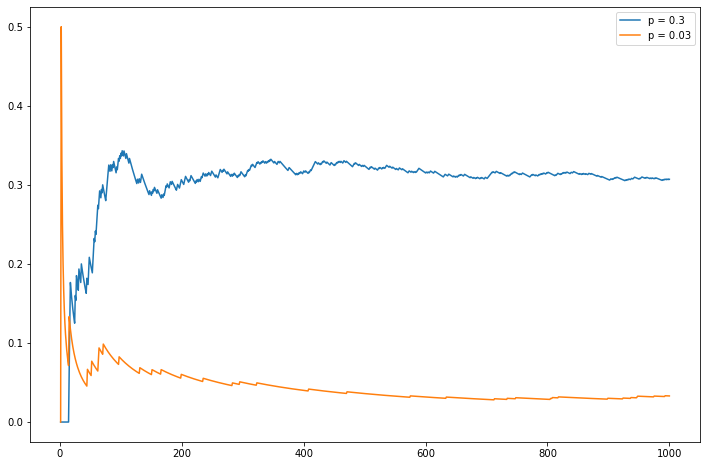
\includegraphics[width=0.9\linewidth,height=0.2\textheight,keepaspectratio]{Figure-02-01}
\end{figure}

\textbf{Exercise 2.10.21 (Computer Experiment)}. Suppose we flip a coin
\(n\) times and let \(p\) denote the probability of heads. Let \(X\) be
the number of heads. We call \(X\) a binomial random variable which is
discussed in the next chapter. Intuition suggests that \(X\) will be
close to \(np\). To see if this is true, we can repeat this experiment
many times and average the \(X\) values. Carry out a simulation and
compare the averages of the \(X\)'s to \(np\). Try this for \(p = .3\)
and \(n = 10, 100, 1000\).

\begin{python}
import numpy as np
from tqdm.notebook import tqdm

B = 50000
p = 0.3

np.random.seed(0)

X1 = np.empty(B)
X2 = np.empty(B)
X3 = np.empty(B)
for i in tqdm(range(B)):
    x1 = np.where(np.random.uniform(low=0,high=1,size=10)<p,1,0)
    x2 = np.where(np.random.uniform(low=0,high=1,size=100)<p,1,0)
    x3 = np.where(np.random.uniform(low=0,high=1,size=1000)<p,1,0)
    X1[i] = np.sum(x1)
    X2[i] = np.sum(x2)
    X3[i] = np.sum(x3)
\end{python}

\begin{python}
print('X1 mean: %.3f' % X1.mean())
print('X1 np:   %.3f' % (0.3 * 10))
print()
print('X2 mean: %.3f' % X2.mean())
print('X2 np:   %.3f' % (0.3 * 100))
print()
print('X3 mean: %.3f' % X3.mean())
print('X3 np:   %.3f' % (0.3 * 1000))
\end{python}

\begin{console}
X1 mean: 3.010
X1 np:   3.000

X2 mean: 30.013
X2 np:   30.000

X3 mean: 300.104
X3 np:   300.000
\end{console}

\begin{python}
import matplotlib.pyplot as plt

plt.figure(figsize=(12, 8))

ax = plt.subplot(3, 1, 1)
ax.hist(X1, density=True, bins=100, label='histogram', color='C0')
ax.vlines(X1.mean(), ymin=0, ymax=5, label=r'$\overline{X}$', color='C1')
ax.vlines(0.3 * 10, ymin=0, ymax=5, label=r'$np$', color='C2')
ax.legend(loc='upper right')
ax.set_title('n = 10')

ax = plt.subplot(3, 1, 2)
ax.hist(X2, density=True, bins=100, label='histogram', color='C0')
ax.vlines(X2.mean(), ymin=0, ymax=0.5, label=r'$\overline{X}$', color='C1')
ax.vlines(0.3 * 100, ymin=0, ymax=0.5, label=r'$np$', color='C2')
ax.legend(loc='upper right')
ax.set_title('n = 100')

ax = plt.subplot(3, 1, 3)
ax.hist(X3, density=True, bins=100, label='histogram', color='C0')
ax.vlines(X3.mean(), ymin=0, ymax=0.05, label=r'$\overline{X}$', color='C1')
ax.vlines(0.3 * 1000, ymin=0, ymax=0.05, label=r'$np$', color='C2')
ax.legend(loc='upper right')
ax.set_title('n = 1000')

plt.tight_layout()
plt.show()
\end{python}

\begin{figure}[H]
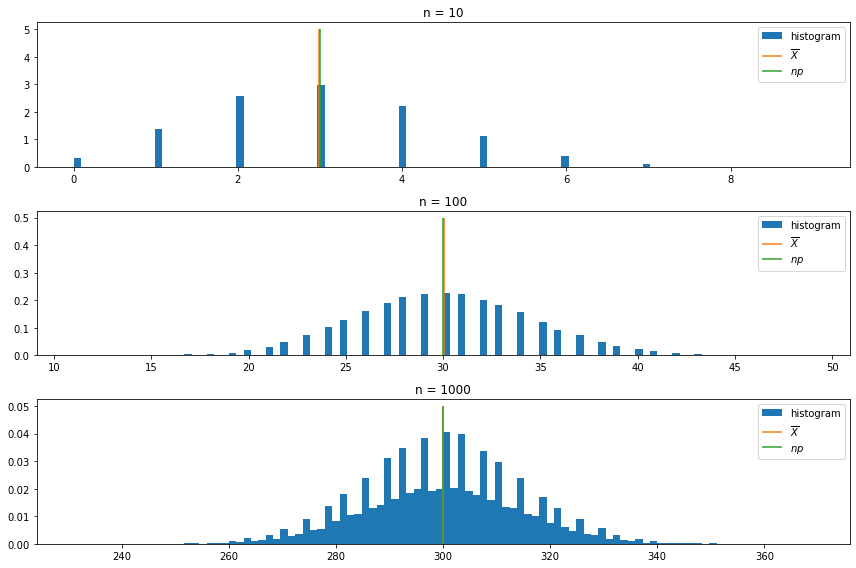
\includegraphics[width=0.9\linewidth,height=0.2\textheight,keepaspectratio]{Figure-02-02}
\end{figure}

\textbf{Exercise 2.10.22 (Computer Experiment)}. Here we will get some
experience simulating conditional probabilities. Consider tossing a fair
die. Let \(A = \{2, 4, 6\}\) and \(B = \{1, 2, 3, 4\}\). Then
\(\mathbb{P}(A) = 1/2\), \(\mathbb{P}(B) = 2/3\) and
\(\mathbb{P}(AB) = 1/3\). Since
\(\mathbb{P}(AB) = \mathbb{P}(A) \mathbb{P}(B)\), the events \(A\) and
\(B\) are independent. Simulate draws from the sample space and verify
that \(\hat{P}(AB) = \hat{P}(A) \hat{P}(B)\) where \(\hat{P}\) is the
proportion of times an event occurred in the simulation. Now find two
events \(A\) and \(B\) that are not independent. Compute \(\hat{P}(A)\),
\(\hat{P}(B)\) and \(\hat{P}(AB)\). Compare the calculated values to
their theoretical values. Report your results and interpret.

\begin{python}
import numpy as np

np.random.seed(0)

B = 10000
results = np.random.randint(low=1, high=7, size=B)

A_hat = np.isin(results, [2, 4, 6])
B_hat = np.isin(results, [1, 2, 3, 4])
AB_hat = np.isin(results, [2, 4])
\end{python}

\begin{python}
import matplotlib.pyplot as plt

nn = np.arange(1, B + 1)


f, (a0, a1) = plt.subplots(2, 1, gridspec_kw={'height_ratios': [3, 1]}, figsize=(12, 8))

a0.plot(nn, np.cumsum(A_hat) / nn, label=r'$\hat{P}(A)$')
a0.plot(nn, np.cumsum(B_hat) / nn, label=r'$\hat{P}(B)$')
a0.plot(nn, np.cumsum(AB_hat) / nn, label=r'$\hat{P}(AB)$')
a0.plot(nn, np.cumsum(A_hat) * np.cumsum(B_hat) / (nn * nn), label=r'$\hat{P}(A) \hat{P}(B)$')
a0.legend(loc='upper right')

a1.plot(nn, np.cumsum(A_hat) * np.cumsum(B_hat) / (nn * nn) - np.cumsum(AB_hat) / nn, 
         label=r'$\hat{P}(A) \hat{P}(B)- \hat{P}(AB)$', color='purple')
a1.legend(loc='upper right')

plt.tight_layout()
plt.show()
\end{python}

\begin{figure}[H]
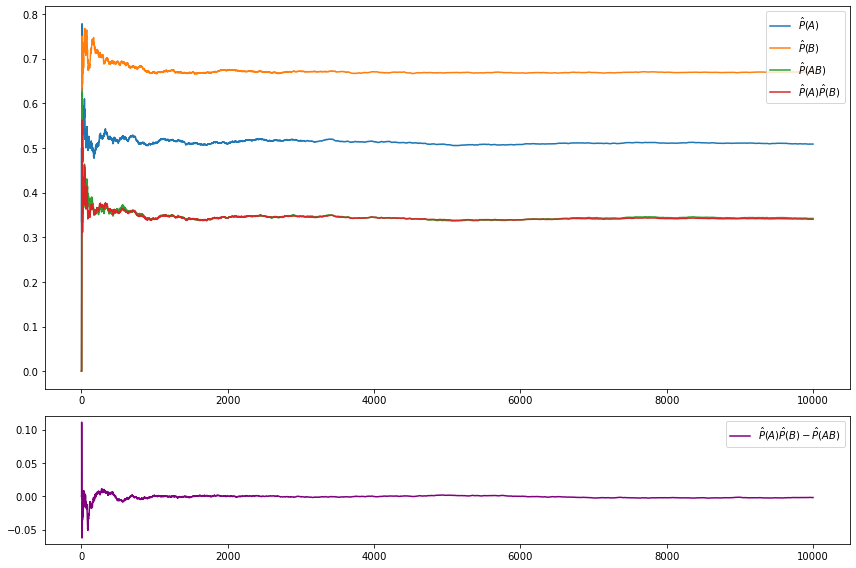
\includegraphics[width=0.9\linewidth,height=0.2\textheight,keepaspectratio]{Figure-02-03}
\end{figure}

For our own choice of non-independent events, let \(A = \{ 2, 4, 6\}\)
and \(B = \{2, 4, 5\}\). Then \(\mathbb{P}(A) = \mathbb{P}(B) = 1/2\)
but \(\mathbb{P}(AB) = 1/3\).

\begin{python}
A_hat = np.isin(results, [2, 4, 6])
B_hat = np.isin(results, [2, 4, 5])
AB_hat = np.isin(results, [2, 4])
\end{python}

\begin{python}
import matplotlib.pyplot as plt

nn = np.arange(1, B + 1)

f, (a0, a1) = plt.subplots(2, 1, gridspec_kw={'height_ratios': [3, 1]}, figsize=(12, 8))

a0.plot(nn, np.cumsum(A_hat) / nn, label=r'$\hat{P}(A)$')
a0.plot(nn, np.cumsum(B_hat) / nn, label=r'$\hat{P}(B)$')
a0.plot(nn, np.cumsum(AB_hat) / nn, label=r'$\hat{P}(AB)$')
a0.plot(nn, np.cumsum(A_hat) * np.cumsum(B_hat) / (nn * nn), label=r'$\hat{P}(A) \hat{P}(B)$')
a0.legend(loc='upper right')

a1.plot(nn, np.cumsum(A_hat) * np.cumsum(B_hat) / (nn * nn) - np.cumsum(AB_hat) / nn, 
         label=r'$\hat{P}(A) \hat{P}(B)- \hat{P}(AB)$', color='purple')
a1.legend(loc='upper right')

plt.tight_layout()
plt.show()
\end{python}

\begin{figure}[H]
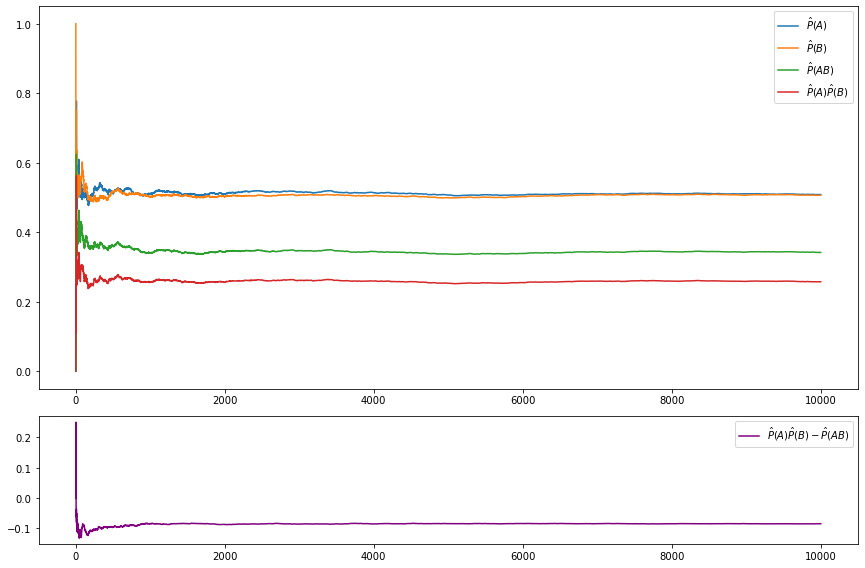
\includegraphics[width=0.9\linewidth,height=0.2\textheight,keepaspectratio]{Figure-02-04}
\end{figure}

As noted, the estimates converges to the theoretical value -- and the
product of the estimates only converge to the estimate of the joint
event in the scenario where the events are independent.



% Chapter 3
\section*{3. Random Variables}\label{random-variables}

\subsection*{3.1 Introduction}\label{introduction:RVs}
A \textbf{random variable} is a mapping \(X : \Omega \rightarrow \R\) that assigns a real number \(X(\omega)\) to each outcome \(\omega\).
\emph{Technically, a random variable must be measurable. See the technical appendix for details.}
Given a random variable \(X\) and a subset \(A\) of the real line, define \(X^{-1}(A) = \{ \omega \in \Omega : X(\omega) \in A \}\) and let
\begin{align*}
\PROB(X \in A) = \PROB(X^{-1}(A)) 
&= \PROB(\{ \omega \in \Omega; X(\omega) \in A \}) 
\\
\PROB(X = x) = \PROB(X^{-1}(x)) 
&= \PROB(\{ \omega \in \Omega; X(\omega) = x \})
\end{align*}
\(X\) denotes a random variable and \(x\) denotes a possible value of \(X\).

\subsection*{3.2 Distribution Functions and Probability Functions}\label{distribution:functions:probability}
The \textbf{cumulative distribution function}, CDF, \(F_X : \R \rightarrow [0, 1]\) of a random variable \(X\) is defined by
\[
F_X(x) = \PROB(X \leq x) 
\]
The following result shows that the CDF completely determines the distribution of a random variable.

\textbf{Theorem 3.7}. Let \(X\) have CDF \(F\) and let \(Y\) have CDF \(G\). If \(F(x) = G(x)\) for all \(x\) then \(\PROB(X \in A) = \PROB(Y \in A)\) for all \(A\).
\emph{Technically, we only have that \(\PROB(X \in A) = \PROB(Y \in A)\) for every measurable event \(A\).}

\textbf{Theorem 3.8}. A function \(F\) that maps the real line to \([0, 1]\) is a CDF for some probability measure \(\PROB\) if and only if if satisfies the following three conditions:
\begin{itemize}[tightlist]
\item
  \(F\) is non-decreasing, i.e.~\(x_{1} < x_{2}\) implies that
  \(F(x_{1}) \leq F(x_{2})\).
\item
  \(F\) is normalized: \(\lim_{n \rightarrow -\infty} F(x) = 0\) and
  \(\lim_{n \rightarrow +\infty} F(x) = 1\).
\item
  \(F\) is right-continuous, i.e.~\(F(x) = F(x^+)\) for all \(x\), where
\end{itemize}
\[
F(x^+) = \lim_{y \rightarrow x, y > x} F(y)
\]
\textbf{Proof}. Suppose that \(F\) is a CDF. Let us show that \(F\) is right-continuous. Let \(x\) be a real number and let \(y_{1}, y_{2}, \dots\) be a sequence of real numbers such that \(y_{1} > y_{2} > \dots\) and \(\lim_{i} y_{i} = x\). Let \(A_{i} = (-\infty, y_{i}]\) and let \(A = (-\infty, x]\). Note that \(A = \inter_{i=1}^{\infty} A_{i}\) and also note that \(A_{1} \supset A_{2} \supset \cdots\). Because the events are monotone, \(\lim_{i} \PROB(A_{i}) = \PROB(\inter_{i} A_{i})\). Thus,
\[
F(x) = \PROB(A) = \PROB(\inter_{i} A_{i}) = \lim_{i} \PROB(A_{i}) = \lim_{i} F(y_{i}) = F(x^+)
\]
Showing that \(F\) is non-decreasing and is normalized is similar. Proving the other direction, that is that \(F\) is non-decreasing, normalized, and right-continuous then it is a CDF for some random variable, uses some deep tools in analysis.
\(X\) is \textbf{discrete} if it takes countably many values
\[
\{ x_{1}, x_{2}, \dots \}
\]
We define the \textbf{probability density function} or
\textbf{probability mass function} for \(X\) by
\[
f_X(x) = \PROB(X = x)
\]
\emph{A set is countable if it is finite or if it can be put in a one-to-one correspondence with the integers.}
Thus, \(f_X(x) \geq 0\) for all \(x \in \R\) and \(\sum_{i} f_X(x_{i}) = 1\). The CDF of \(X\) is related to the PDF by
\[
F_X(x) = \PROB(X \leq x) = \sum_{x_{i} \leq x} f_X(x_{i})
\]
Sometimes we write \(f_X\) and \(F_X\) simply as \(f\) and \(F\).
A random variable \(X\) is \textbf{continuous} if there exists a function \(f_X\) such that \(f_X(x) \geq 0\) for all \(x\), \(\int_{-\infty}^{\infty} f_X(x) dx = 1\), and for every \(a \leq b\),
\[
\PROB(a < X < b) = \int_a^{b} f_X(x) dx
\]
The function \(f_X\) is called the \textbf{probability density function}. We have that
\[
F_X(x) = \int_{-\infty}^x f_X(t) dt
\]
and \(f_X(x) = F'_X(x)\) at all points \(x\) at which \(F_X\) is differentiable.
Sometimes we shall write \(\int f(x) dx\) or simply \(\int f\) to mean \(\int_{-\infty}^{\infty} f(x) dx\).
\textbf{Warning}: Note that if \(X\) is continuous then \(\PROB(X = x) = 0\) for every \(x\). We only have \(f(x) = \PROB(X = x)\) for discrete random variables; we get probabilities from a PDF by integrating.
\textbf{Lemma 3.15}. Let \(F\) be the CDF for a random variable \(X\).
Then:
\begin{itemize}
\item
  \(\PROB(X = x) = F(x) - F(x^-)\) where
  \(F(x^-) = \lim_{y \uparrow x} F(y)\)
\item
  \(\PROB(x < X \leq y) = F(y) - F(x)\)
\item
  \(\PROB(X > x) = 1 - F(x)\)
\item
  If \(X\) is continuous then
  \[
 \PROB(a < X < b) 
  = \PROB(a \leq X < b) 
  = \PROB(a < X \leq b) 
  = \PROB(a \leq X \leq b)
\]
\end{itemize}
It is also useful to define the inverse CDF (or quantile function).
Let \(X\) be a random variable with CDF \(F\). The \textbf{inverse CDF} or \textbf{quantile function} is defined by
\[
F^{-1}(q) = \inf \{ x : F(x) \ge q \}
\]
for \(q \in [0, 1]\). If \(F\) is strictly increasing and continuous then \(F^{-1}(q)\) is the unique real number \(x\) such that \(F(x) = q\).
We call \(F^{-1}(1/4)\) the first quartile, \(F^{-1}(1/2)\) the median (or second quartile), and \(F^{-1}(3/4)\) the third quartile.
Two random variables \(X\) and \(Y\) are \textbf{equal in distribution} -- denoted \(X \overset{d}= Y\) -- if \(F_X(x) = F_Y(x)\) for all \(x\). This does not mean that \(X\) and \(Y\) are equal. Rather, it means that probability statements about \(X\) and \(Y\) will be the same.

\subsection*{3.3 Some Important Discrete Random Variables}\label{some-important-discrete-random-variables}
\textbf{Notation}: It is traditional to write \(X \sim F\) to indicate that \(X\) has distribution \(F\). 
% This is an unfortunate notation since the symbol \(\sim\) is also used to denote an approximation. The notation is so pervasive we are stuck with it.
% Note: We use \(A \approx B\) to denote approximation. 
%The LaTeX macros hint at this common usage: \texttt{\textbackslash{}sim} for \(\sim\), and \texttt{\textbackslash{}approx} for \(\approx\).}
\paragraph{The Point Mass Distribution}\label{the-point-mass-distribution}
\(X\) has a point mass distribution at \(a\), denoted \(X \sim \delta_a\), if \(\PROB(X = a) = 1\), in which case
\[
F(x) = 
\begin{cases}
0 &\text{if } x < a 
\\[
1ex]
1 &\text{if } x \geq a
\end{cases}
\]
The probability mass function is \(f(x) = I(x = a)\), which takes value $1$ if \(x = a\) and 0 otherwise.
\paragraph{The Discrete Uniform Distribution}\label{the-discrete-uniform-distribution}
Let \(k > 1\) be a given integer. Suppose that \(X\) has probability mass function given by
\[
f(x) = 
\begin{cases}
1/k &\text{for } x = 1, \dots, k 
\\[
1ex]
0 &\text{otherwise}
\end{cases}
\]
We say that \(X\) has a uniform distribution on \(\{ 1, \dots, k \}\).
\paragraph{The Bernoulli Distribution}\label{the-bernoulli-distribution}
Let \(X\) represent a coin flip. Then \(\PROB(X = 1) = p\) and \(\PROB(X = 0) = 1 - p\) for some \(p \in [0, 1]\). We say that \(X\) has a Bernoulli distribution, denoted \(X \sim \text{Bernoulli}(p)\). The probability mass function is \(f(x) = p^x (1 - p)^{1 - x}\) for \(x \in \{ 0, 1 \}\).
\paragraph{The Binomial Distribution}\label{the-binomial-distribution}
Suppose we have a coin which falls heads with probability \(p\) for some \(0 \leq p \leq 1\). Flip the coin \(n\) times and let \(X\) be the number of heads. Assume that the tosses are independent. Let \(f(x) = \PROB(X = x)\) be the mass function. It can be shown that
\[
f(x) = 
\begin{cases}
\binomial{n}{x} p^x (1 - p)^{n - x} &\text{for } x= 0, \dots, n 
\\[
1ex]
0 &\text{otherwise}
\end{cases}
\]
A random variable with this mass function is called a Binomial random variable, and we write \(X \sim \text{Binomial}(n, p)\). If \(X_{1} \sim \text{Binomial}(n, p_{1})\) and \(X_{2} \sim \text{Binomial}(n, p_{2})\) then \(X_{1} + X_{2} \sim \text{Bimomial}(n, p_{1} + p_{2})\).
Note that \(X\) is a random variable, \(x\) denotes a particular value of the random variable, and \(n\) and \(p\) are \textbf{parameters}, that is, fixed real numbers.
\paragraph{The Geometric Distribution}\label{the-geometric-distribution}
\(X\) has a geometric distribution with parameter \(p \in (0, 1)\), denoted \(X \sim \text{Geom}(p)\), if
\[
\PROB(X = k) = p(1 - p)^{k - 1}, \quad k \geq 1
\]
We have that
\[
\sum_{k=1}^{\infty} \PROB(X = k) = p \sum_{k=1}^{\infty} (1 - p)^{k} = \frac{p}{1 - (1 - p)} = 1
\]
\(X\) counts the number of flips needed until the first head.
\paragraph{The Poisson Distribution}\label{the-poisson-distribution}
\(X\) has a Poisson distribution with parameter \(\lambda\), denoted \(X \sim \text{Poisson}(\lambda)\), if
\[
f(x) = e^{-\lambda} \frac{\lambda^x}{x!}, \quad x \geq 0
\]
Note that
\[
\sum_{x=1}^{\infty} f(x) 
= e^{-\lambda} \sum_{x=1}^{\infty} \frac{\lambda^x}{x!} 
= e^{-\lambda} e^\lambda = 1
\]
The Poisson distribution is often used as a model for counts of rare events like radioactive decay and traffic accidents. If \(X_{1} \sim \text{Poisson}(n, \lambda_{1})\) and \(X_{2} \sim \text{Poisson}(n, \lambda_{2})\) then \(X_{1} + X_{2} \sim \text{Poisson}(n, \lambda_{1} + \lambda_{2})\).
\textbf{Warning}: We defined random variables to be mappings from a sample space \(\Omega\) to \(\R\) but we did not mention sample space in any of the distributions above. Construct a sample space explicitly for a Bernoulli random variable. Let \(\Omega = [0, 1]\), and define \(\PROB\) to satisfy \(\PROB([a, b]) = b - a\) for \(0 \leq a \leq b \leq 1\). Fix \(p \in [0, 1]\) and define
\[
X(\omega) = 
\begin{cases}
1 &\text{if }\omega \leq p 
\\
0 &\text{if }\omega > p
\end{cases}
\]
Then \(\PROB(X = 1) = \PROB(\omega \leq p) = \PROB([0, p]) = p\) and \(\PROB(X = 0) = 1 - p\). Thus, \(X \sim \text{Bernoulli}(p)\). We could do this for all of the distributions defined above. In practice, we think of a random variable like a random number but formally it is a mapping defined on some sample space.

\subsection*{3.4 Some Important Continuous Random Variables}\label{some-important-continuous-random-variables}
\paragraph{The Uniform Distribution}\label{the-uniform-distribution}
\(X\) has a uniform distribution with parameters \(a\) and \(b\), denoted \(X \sim \text{Uniform}(a, b)\), if
\[
f(x) = 
\begin{cases}
\Frac{1}{b - a} &\text{for } x \in [a, b]
\\[
1ex]
0 &\text{otherwise}
\end{cases}
\]
where \(a < b\). The CDF is
\[
F(x) = 
\begin{cases}
0 &\text{if } x < a 
\\[
1ex]
\Frac{x - a}{b - a} &\text{if } x \in [a, b] 
\\[
1ex]
1 &\text{if } x > b
\end{cases}
\]
\paragraph{Normal (Gaussian)}\label{normal-gaussian}
\(X\) has a Normal (or Gaussian) distribution with parameters \(\mu\) and \(\sigma\), denoted by \(X \sim N(\mu, \sigma^{2})\), if
\[
f(x) = \frac{1}{\sigma \sqrt{2 \pi}} \exp \left\{ -\frac{1}{2} \left( \frac{x - \mu}{\sigma} \right)^{2}\right\}, \quad x \in \R
\]
where \(\mu \in \R\) and \(\sigma > 0\). Later we shall see that \(\mu\) is the ``center'' (or mean) of the distribution and that \(\sigma\) is the ``spread'' (or standard deviation) of the distribution. The Normal distribution plays an important role in probability and statistics. Many phenomena have approximately Normal distributions. Later, we shall see that the distribution of a sum of random variables can be approximated by a Normal distribution (the central limit Theorem).
We say that \(X\) has a \textbf{standard Normal distribution} if \(\mu = 0\) and \(\sigma = 1\). The standard Normal random variable is denoted by \(Z\). The PDF and the CDF of the standard Normal are denoted by \(\phi(z)\) and \(\Phi(z)\). The PDF is plotted below.

\begin{python}
import numpy as np
from scipy.stats import norm
import matplotlib.pyplot as plt
xx = np.arange(-5, 5, step=0.01)
plt.figure(figsize=(12, 8))
plt.plot(xx, norm.pdf(xx, loc=0, scale=1))
plt.title('Standard Normal PDF')
plt.show()
\end{python}

\begin{figure}[H]
\centering
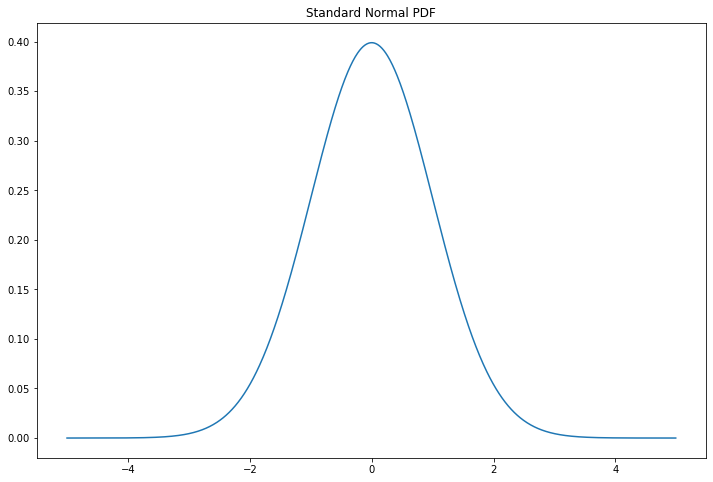
\includegraphics{Figure-03-01}
\end{figure}

There is no closed-form expression for \(\Phi\). Here are some useful facts:
\begin{itemize}
\item
  If \(X \sim N(\mu, \sigma^{2})\) then
  \(Z = (X - \mu) / \sigma \sim N(0, 1)\)
\item
  If \(Z \sim N(0, 1)\) then
  \(X = \mu + \sigma Z \sim N(\mu, \sigma^{2})\)
\item
  If \(X_{i} \sim N(\mu_{i}, \sigma_{i}^{2})\), \(i = 1, \dots, n\) are
  independent then
  \[
\sum_{i=1}^{n} X_{i} \sim N \left(\sum_{i=1}^{n} \mu_u, \sum_{i=1}^{n} \sigma_{i}^{2} \right)
\]
\end{itemize}
It follows from the first fact that if \(X \sim N(\mu, \sigma^{2})\) then
\[
\PROB(a < X < b) 
= \PROB\left( \frac{a - \mu}{\sigma} < Z < \frac{b - \mu}{\sigma} \right) 
= \Phi \left( \frac{b - \mu}{\sigma} \right) - \Phi \left( \frac{a - \mu}{\sigma} \right)
\]
Thus we can compute any probabilities we want as long as we can compute the CDF \(\Phi(z)\) of the standard Normal. All statistical and computing packages will compute \(\Phi(z)\) and \(\Phi^{-1}(q)\).
\paragraph{Exponential Distribution}\label{exponential-distribution}
\(X\) has an exponential distribution with parameter \(\beta\), denoted by \(X \sim \text{Exp}(\beta)\), if
\[
f(x) = \frac{1}{\beta} e^{-x / \beta}, \quad x > 0
\]
where \(\beta > 0\). The exponential distribution is used to model the lifetimes of electronic components and the waiting times between rare events.
\paragraph{Gamma Distribution}\label{gamma-distribution}
For \(\alpha > 0\), the \textbf{Gamma function} is defined by \(\Gamma(\alpha) = \int_{0}^{\infty} y^{\alpha - 1} e^{-y} dy\). \(X\) has a Gamma distribution with parameters \(\alpha\) and \(\beta\), denoted by \(X \sim \text{Gamma}(\alpha, \beta)\), if
\[
f(x) = \frac{1}{\beta^\alpha \Gamma(\alpha)} x^{\alpha - 1} e^{-x / \beta}, \quad x > 0
\]
where \(\alpha, \beta > 0\). The exponential distribution is just a \(\text{Gamma}(1, \beta)\) distribution. If \(X_{i} \sim \text{Gamma}(\alpha_{i}, \beta)\) are independent, then \(\sum_{i=1}^{n} X_{i} \sim \text{Gamma}\left( \sum_{i=1}^{n} \alpha_{i}, \beta \right)\).
\paragraph{Beta Distribution}\label{beta-distribution}
\(X\) has Beta distribution with parameters \(\alpha > 0\) and \(\beta > 0\), denoted by \(X \sim \text{Beta}(\alpha, \beta)\), if
\[
f(x) = \frac{\Gamma(\alpha + \beta)}{\Gamma(\alpha) \Gamma(\beta)} x^{\alpha - 1} (1 - x)^{\beta - 1}, \quad 0 < x < 1
\]
\paragraph{\texorpdfstring{\(t\) and Cauchy Distribution}{t and Cauchy Distribution}}\label{t-and-cauchy-distribution}
\(X\) has a \(t\) distribution with \(\nu\) degrees of freedom -- denoted \(X \sim t_\nu\), if
\[
f(x) = \frac{1}{\sqrt{\nu \pi}} \frac{\Gamma\left( \frac{\nu + 1}{2} \right)}{\Gamma\left( \frac{\nu}{2} \right)} \frac{1}{\left(1 + \frac{x^{2}}{\nu} \right)^{(\nu + 1) / 2}} 
\]
The \(t\) distribution is similar to a Normal but it has thicker tails. In fact, the Normal corresponds to a \(t\) with \(\nu = \infty\). The Cauchy distribution is a special case of the \(t\) distribution corresponding to \(\nu = 1\). The density is
\[
f(x) = \frac{1}{\pi (1 + x^{2})}
\]
\paragraph{\texorpdfstring{The \(\chi^{2}\) Distribution}{The \textbackslash chi^{2} Distribution}}\label{chi2:dist}
\(X\) has a \(\chi^{2}\) distribution with \(p\) degrees of freedom -- denoted \(X \sim \chi_{p}^{2}\) -- if
\[
f(x) = \frac{1}{\Gamma\left(\frac{p}{2}\right) 2^{\frac{p}{2}}} x^{\frac{p}{2} - 1} e^{-\frac{x}{2}}, \quad x > 0 
\]
If \(Z_{1}, Z_{2}, \dots\) are independent standard Normal random variables then \(\sum_{i=1}^p Z_{i}^{2} \sim \chi_{p}^{2}\).

\subsection*{3.5 Bivariate Distributions}\label{bivariate-distributions}
Given a pair of discrete random variables \(X\) and \(Y\), define the \textbf{joint mass function} by \(f(x, y) = \PROB(X = x \text{ and } Y = y)\). From now on, we write \(\PROB(X = x \text{ and } Y = y)\) as \(\PROB(X = x, Y = y)\). We write \(f\) as \(f_{X, Y}\) when we want to be more explicit.
In the continuous case, we call a function \(f(x, y)\) a PDF for the random variables \((X, Y)\) if:  \(f(x, y) \geq 0\) for all \((x, y)\), \( \int_{-\infty}^{\infty}\int_{-\infty}^{\infty} f(x, y) dx dy = 1\) 
For any set \(A \subset \R \times \R\), \(\PROB((X, Y) \in A) = \int \int_A f(x, y) \; dx dy\)
In the continuous or discrete case, we define the joint CDF as 
\(F_{X, Y}(x, y) = \PROB(X \leq x, Y \leq y)\).

\subsection*{3.6 Marginal Distributions}\label{marginal-distributions}
If \((X, Y)\) have joint distribution with mass function \(f_{X, Y}\), then the \textbf{marginal mass function} for \(X\) is defined by
\[
f_X(x) = \PROB(X = x) = \sum_y \PROB(X = x, Y = y) = \sum_y f(x, y)
\]
and the \textbf{marginal mass function} for \(Y\) is defined by
\[
f_Y(y) = \PROB(Y = y) = \sum_x \PROB(X = x, Y = y) = \sum_x f(x, y) 
\]
For continuous random variables, the marginal densities are
\[
f_X(x) = \int f(x, y) \; dy \quad \text{and} \quad f_Y(y) = \int f(x, y) \; dx 
\]
The corresponding marginal CDFs are denoted by \(F_X\) and \(F_Y\).

\subsection*{3.7 Independent Random Variables}\label{independent-random-variables}
Two random variables \(X\) and \(Y\) are \textbf{independent} if, for every \(A\) and \(B\),
\[
\PROB(X \in A, Y \in B) = \PROB(X \in A) \PROB(Y \in B)
\]
We write \(X \ci Y\).
In principle, to check whether \(X\) and \(Y\) are independent we need to check the equation above for all subsets \(A\) and \(B\). Fortunately, we have the following result which we state for continuous random variables though it is true for discrete random variables too.

\textbf{Theorem 3.30}. Let \(X\) and \(Y\) have joint PDF \(f_{X, Y}\). Then \(X \ci Y\) if and only if \(f_{X, Y}(x, y) = f_X(x) f_Y(y)\) for all values \(x\) and \(y\).
\emph{The statement is not rigorous because the density is defined only up to sets of measure 0.}
The following result is helpful for verifying independence.

\textbf{Theorem 3.33}. Suppose that the range of \(X\) and \(Y\) is a (possibly infinite) rectangle. If \(f(x, y) = g(x) h(y)\) for some functions \(g\) and \(h\) (not necessarily probability density functions) then \(X\) and \(Y\) are independent.

\subsection*{3.8 Conditional Distributions}\label{conditional-distributions}
The \textbf{conditional probability mass function} is
\[
f_{X | Y}(x | y) = \PROB(X = x | Y = y) = \frac{\PROB(X = x, Y = y)}{\PROB(Y = y)} = \frac{f_{X, Y}(x, y)}{f_Y(y)}
\]
if \(f_Y(y) > 0\).
For continuous random variables, the \textbf{conditional probability density function} is
\[
f_{X | Y}(x | y) = \frac{f_{X, Y}(x, y)}{f_Y(y)}
\]
assuming that \(f_Y(y) > 0\). Then,
\[
\PROB(X \in A | Y = y) = \int_A f_{X | Y}(x | y) \; dx
\]
\emph{We are treading in deep water here. When we compute \(\PROB(X \in A | Y = y)\) in the continuous case we are conditioning on the event \(\PROB(Y = y)\) which has probability $0$. We avoid this problem by defining things in terms of the PDF. The fact that this leads to a well-defined theory is proved in more advanced courses. We simply take it as a definition.}

\subsection*{3.9 Multivariate Distributions and IID Samples}\label{multivariate-distributions-and-iid-samples}
Let \(X = (X_{1}, \dots, X_{n})\) where the \(X_{i}\)s are random variables. We call \(X\) a \textbf{random vector}. Let \(f(x_{1}, \dots, x_{n})\) denote the PDF. It is possible to define their marginals, conditionals, etc. much the same way as in the bivariate case. We say that \(X_{1}, \dots, X_{n}\) are independent if, for every \(A_{1}, \dots, A_{n}\),
\[
\PROB(X_{1} \in A_{1}, \dots, X_{n} \in A_{n}) = \prod_{i=1}^{n} \PROB(X_{i} \in A_{i})
\]
It suffices to check that \(f(x_{1}, \dots, x_{n}) = \prod_{i=1}^{n} f_{X_{i}}(x_{i})\). If \(X_{1}, \dots, X_{n}\) are independent and each has the same marginal distribution with density \(f\), we say that \(X_{1}, \dots, X_{n}\) are IID (independent and identically distributed). We shall write this as \(X_{1}, \dots, X_{n} \sim f\) or, in terms of the CDF, \(X_{1}, \dots, X_{n} \sim F\). This means that \(X_{1}, \dots, X_{n}\) are independent draws from the same distribution. We also call \(X_{1}, \dots, X_{n}\) a \textbf{random sample} from \(F\).

\subsection*{3.10 Two Important Multivariate Distributions}\label{two-important-multivariate-distributions}
\paragraph{Multinomial Distribution}\label{multinomial-distribution}
The multivariate version of the Binomial is called a Multinomial.
Consider drawing a ball from an urn which has balls of \(k\) different
colors. Let \(p = (p_{1}, \dots, p_{k})\) where \(p_{j} \geq 0\) and
\(\sum_{j=1}^{k} p_{j} = 1\) and suppose that \(p_{j}\) is the probability of
drawing a ball of color \(j\). Draw \(n\) times (independent draws with
replacement) and let \(X = (X_{1}, \dots, X_{k})\), where \(X_{j}\) is the
number of times that color \(j\) appears. Hence,
\(n = \sum_{j=1}^{k} X_{j}\). We say that \(X\) has a Multinomial
distribution with parameters \(n\) and \(p\), denoted
\(X \sim \text{Multinomial}(n, p)\). The probability function is
\[
f(x) = \binom{n}{x_{1} \cdots x_{k}} p_{1}^{x_{1}} \cdots p_{k}^{x_{k}}
\]
where
\[
\binom{n}{x_{1} \cdots x_{k}} = \frac{n!}{x_{1}! \cdots x_{k}!}
\]
\textbf{Lemma 3.41}. Suppose that \(X \sim \text{Multinomial}(n, p)\)
where \(X = (X_{1}, \dots, X_{k})\) and \(p = (p_{1}, \dots, p_{k})\). The
marginal distribution of \(X_{j}\) is \(\text{Binomial}(n, p_{j})\).
\paragraph{Multivariate Normal}\label{rv:multivariate:normal}
The univariate Normal had two parameters, \(\mu\) and \(\sigma\). In the
multivariate vector, \(\mu\) is a vector and \(\sigma\) is replaced by a
matrix \(\Sigma\). To begin, let
\[
Z = \begin{pmatrix}
Z_{1} \\
\vdots \\
Z_{k}
\end{pmatrix}
\]
where \(Z_{1}, \dots, Z_{k} \sim N(0, 1)\) are independent. The density of
\(Z\) is
\[
f(z) = \prod_{i=1}^{k} f(z_{i}) 
= \frac{1}{(2 \pi)^{k/2}} \exp \left\{ -\frac{1}{2} \sum_{j=1}^{k} z_{j}^{2} \right\} 
= \frac{1}{(2 \pi)^{k/2}} \exp \left\{ -\frac{1}{2} z^T z \right\} 
\]
We say that \(Z\) has a standard multivariate Normal distribution, denoted \(Z \sim N(0, I)\) where it is understood that \(0\) represents a vector of \(k\) zeroes and \(I\) is the \(k \times k\) identity matrix.
More generally, a vector \(X\) has multivariate Normal distribution, denoted by \(X \sim N(\mu, \Sigma)\), if it has density
\[
f(x; \mu, \Sigma) = \frac{1}{(2 \pi)^{k/2} \det(\Sigma)^{1/2}} \exp \left\{ - \frac{1}{2} (x - \mu)^T \Sigma^{-1} (x - \mu) \right\}
\]
where \(\det(\cdot)\) denotes the determinant of a matrix, \(\mu\) is a vector of length \(k\), and \(\Sigma\) is a \(k \times k\) symmetric, positive definite matrix. Setting \(\mu = 0\) and \(\Sigma = I\) gives back the standard Normal.
\emph{A matrix \(\Sigma\) is positive definite if, for all non-zero vectors \(x\), \(x^T \Sigma x > 0\).}
Since \(\Sigma\) is symmetric and positive definite, it can be shown that there exists a matrix \(\Sigma^{1/2}\) -- called the square root of \(\Sigma\) -- with the following properties:
\begin{itemize}[tightlist]
\item
  \(\Sigma^{1/2}\) is symmetric
\item
  \(\Sigma = \Sigma^{1/2} \Sigma^{1/2}\)
\item
  \(\Sigma^{1/2}\Sigma^{-1/2} = \Sigma^{-1/2}\Sigma^{1/2} = I\), where
  \(\Sigma^{1/2} = \left(\Sigma^{1/2}\right)^{-1}\)
\end{itemize}

\textbf{Theorem 3.42}. If \(Z \sim N(0, I)\) and
\(X = \mu + \Sigma^{1/2} Z\) then \(X \sim N(\mu, \Sigma)\). Conversely,
if \(X \sim N(\mu, \Sigma)\), then
\(\Sigma^{-1/2}(X - \mu) \sim N(0, I)\).
Suppose we partition a random Normal vector \(X\) as \(X = (X_a, X_b)\),
and we similarly partition
\[
\mu = \begin{pmatrix}\mu_a & \mu_b \end{pmatrix} 
\quad
\Sigma = \begin{pmatrix}
\Sigma_{aa} & \Sigma_{ab} \\
\Sigma_{ba} & \Sigma_{bb}
\end{pmatrix}
\]

\textbf{Theorem 3.43}. Let \(X \sim N(\mu, \Sigma)\). Then:
\begin{enumerate}[label={\arabic*.}]
\item
  The marginal distribution of \(X_a\) is
  \(X_a \sim N(\mu_a, \Sigma_{aa})\).
\item
  The conditional distribution of \(X_b\) given \(X_a = x_a\) is
  \[
 X_b | X_a = x_a \sim N \left( \mu_b + \Sigma_{ba}\Sigma_{aa}^{-1}(x_a - \mu_a), \Sigma_{bb} - \Sigma_{ba} \Sigma_{aa}^{-1} \Sigma_{ab} \right)
\]
\item
  If \(a\) is a vector then \(a^T X \sim N(a^T \mu, a^T \Sigma a)\)
\item
  \(V = (X - \mu)^T \Sigma^{-1} (X - \mu) \sim \chi_{k}^{2}\)
\end{enumerate}

\subsection*{3.11 Transformations of Random
Variables}\label{transformations-of-random-variables}
Suppose that \(X\) is a random variable with PDF \(f_X\) and CDF
\(F_X\). Let \(Y = r(X)\) be a function of \(X\), such as \(Y = X^{2}\) or
\(Y = e^X\). We call \(Y = r(X)\) a transformation of \(X\). How do we
compute the PDF and the CDF of \(Y\)? In the discrete case, the answer
is easy. The mass function of \(Y\) is given by
\[
f_Y(y) = \PROB(Y = y) = \PROB(r(X) = y) = \PROB(\{x; r(x) = y\}) = \PROB(X \in r^{-1}(y))
\]
The continuous case is harder. There are 3 steps for finding \(f_Y\):
\begin{enumerate}[label={\arabic*.}]
\item
  For each \(y\), find the set \(A_y = \{ x : r(x) \leq y \}\).
\item
  Find the CDF
  \[
F_Y(y) = \PROB(Y \leq y) = \PROB(r(X) \leq y) = \PROB(\{x ; r(x) \leq y \}) = \int_{A_y} f_X(x) dx
\]
\item
  The PDF is \(f_Y(y) = F'_Y(y)\).
\end{enumerate}
When \(r\) is strictly monotone increasing or strictly monotone
decreasing then \(r\) has an inverse \(s = r^{-1}\) and in this case one
can show that
\[
f_Y(y) = f_X(s(y)) \;\Bigg| \frac{ds(y)}{dy} \Bigg|
\]

\subsection*{3.12 Transformation of Several Random
Variables}\label{transformation-of-several-random-variables}
In some cases we are interested in the transformation of several random
variables. For example, if \(X\) and \(Y\) are given random variables,
we might want to know the distribution of \(X / Y\), \(X + Y\),
\(\max \{ X, Y \}\) or \(\min \{ X, Y \}\). Let \(Z = r(X, Y)\). The
steps for finding \(f_Z\) are the same as before:
\begin{enumerate}[tightlist,label={\arabic*.}]
\item
  For each \(z\), find the set \(A_z = \{ (x, y) : r(x, y) \leq z \}\).
\item
  Find the CDF
\end{enumerate}
\[
F_Z(z) = \PROB(Z \leq z) = \PROB(r(X, Y) \leq z) = \PROB(\{ (x, y) : r(x, y) \leq z \})
  = \int \int_{A_z} f_{X, Y}(x, y) \; dx dy 
\]
\begin{enumerate}[tightlist,label={\arabic*.},resume]
\item
  Find \(f_Z(z) = F'_Z(z)\).
\end{enumerate}

\subsection*{3.13 Technical Appendix}
Recall that a probability measure \(\PROB\) is defined on a
\(\sigma\)-field \(\mathcal{A}\) of a sample space \(\Omega\). A random
variable \(X\) is \textbf{measurable} map
\(X : \Omega \rightarrow \R\). Measurable means that, for every
\(x\), $\{ \omega : X(\omega) \leq x \} \in \mathcal{A} $.

\subsection*{3.14 Exercises}

\textbf{Exercise 3.14.1}. Show that
\[
\PROB(X = x) = F(x^+) - F(x^-)
\]
and
\[
F(x_{2}) - F(x_{1}) = \PROB(X \leq x_{2}) - \PROB(X \leq x_{1})
\]

\textbf{Solution}.
By definition, \(F(x_{2}) = \PROB(X \leq x_{2})\) and
\(F(x_{1}) = \PROB(X \leq x_{1})\), so the second equation is
immediate.
Also by definition,
\[
F(x^+) = \lim_{y \rightarrow x, y > x} F(y) = \lim_{y \rightarrow x, y > x} \PROB(X \leq y) 
= \PROB(\exists y : X \leq y, y > x) 
= \PROB(X \leq x)
\]
and
\[
F(x^-) = \lim_{y \rightarrow x, y < x} F(y) = \lim_{y \rightarrow x, y > x} \PROB(X \leq y) 
= \PROB(\exists y : X \leq y, y < x)
= \PROB(X < x)
\]
and so
\[
F(x^+) - F(x^-) = \PROB(X \leq x) - \PROB(X < x) = \PROB(X(\omega) \in \{x : X(\omega) \leq x \} - \{x: X(\omega) < x \}) = \PROB(X = x)
\]

\textbf{Exercise 3.14.2}. Let \(X\) be such that
\(\PROB(X = 2) = \PROB(X = 3) = 1/10\) and
\(\PROB(X = 5) = 8/10\). Plot the CDF \(F\). Use \(F\) to find
\(\PROB(2 < X \leq 4.8)\) and \(\PROB(2 \leq X \leq 4.8)\).

\textbf{Solution}.

\begin{python}
import numpy as np
import matplotlib.pyplot as plt
plt.figure(figsize=(12, 8))
# Draw horizontal lines
for xmin, xmax, y in [(0, 2, 0), (2, 3, 1/10), (3, 5, 2/10), (5, 10, 1)]:
    plt.hlines(y, xmin, xmax, color='C0', linestyle='solid')
    
# Draw vertical lines
for ymin, ymax, x in [(0, 1/10, 2), (1/10, 2/10, 3), (2/10, 1, 5)]:
    plt.vlines(x, ymin, ymax, color='C0', linestyle='dashed')
    
# Mark open intervals
plt.scatter([2, 3, 5], [0, 1/10, 2/10], color='C0', facecolor='white', zorder=10, linewidth=2)
# Mark close intervals
plt.scatter([2, 3, 5], [1/10, 2/10, 1], color='C0', facecolor='C0', zorder=10, linewidth=2)
plt.xlabel('x')
plt.ylabel('F(x)')
plt.show()
\end{python}

\begin{figure}[H]
\centering
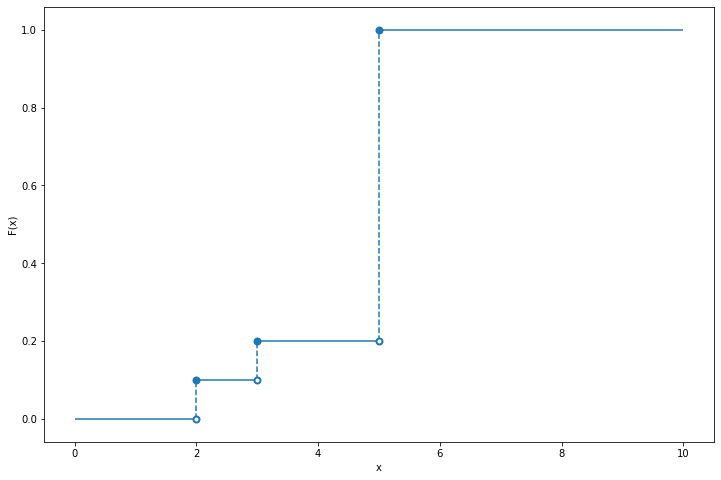
\includegraphics{Figure-03-02}
\end{figure}

\begin{align*}
\PROB(2 < X \leq 4.8) 
& = F(4.8) - F(2) = 0.2 - 0.1 = 0.1
\\
\PROB(2 \leq X \leq 4.8) 
& = F(4.8) - F(2^{-}) = 0.2 - 0 = 0.2
\end{align*}

\textbf{Exercise 3.14.3}. Prove Lemma 3.15.
Let \(F\) be the CDF for a random variable \(X\). Then:
\begin{itemize}
\item
  \(\PROB(X = x) = F(x) - F(x^-)\) where
  \(F(x^-) = \lim_{y \uparrow x} F(y)\)
\item
  \(\PROB(x < X \leq y) = F(y) - F(x)\)
\item
  \(\PROB(X > x) = 1 - F(x)\)
\item
  If \(X\) is continuous then
  \[
\PROB(a < X < b) = \PROB(a \leq X < b) = \PROB(a < X \leq b) = \PROB(a \leq X \leq b)
\]
\end{itemize}

\textbf{Solution}.
Proof of first statement:
\[
F(x) - F(x^{-}) = \PROB(X \leq x) - \PROB(X < x) = \PROB(\{\omega : X(\omega) \leq x\} - \{\omega : X(\omega) < x\}) = \PROB(X = x)
\]
Proof of second statement:
\[
\PROB(x < X \leq y) = \PROB(\{\omega : X(\omega) \leq y\} - \{\omega : X(\omega) \leq x\}) = \PROB(X \leq y) - \PROB(X \leq x) = F(y) - F(x)
\]
Proof of third statement:
\[
\PROB(X > x) = \PROB(\{\omega: X(\omega) > x\}) = \PROB(\{\omega: X(\omega) \leq x\}^{c}) = 1 - \PROB(X \leq x) = 1 - F(x)
\]
Proof of fourth statement:
If \(F\) is continuous, then
\(\PROB(X = a) = \PROB(X = b) = 0\), and so
\begin{align*}
\PROB(a < X \leq b) 
&= \PROB(a < X < b) + \PROB(X = b) = \PROB(a < X < b) 
\\
\PROB(a \leq X < b) 
&= \PROB(X = a) + \PROB(a < X < b) = \PROB(a < X < b) 
\\
\PROB(a \leq X \leq b) 
&= \PROB(X = a) + \PROB(a < X < b) + \PROB(X = b) 
 = \PROB(a < X < b)
\end{align*}

\textbf{Exercise 3.14.4}. Let \(X\) have probability density function
\[
f_X(x) = 
\begin{cases}
1/4 &\text{if } 0 < x < 1 \\
3/8 &\text{if } 3 < x < 5 \\
0   &\text{otherwise}
\end{cases}
\]
\textbf{(a)} Find the cumulative distribution function of \(X\).
\textbf{(b)} Let \(Y = 1 / X\). Find the probability density function
\(f_Y(y)\) for \(Y\). Hint: Consider three cases,
\(\frac{1}{5} \leq y \leq \frac{1}{3}\), \(\frac{1}{3} \leq y \leq 1\),
and \(y \geq 1\).

\textbf{Solution}.
\textbf{(a)}
\[
F_X(x) = 
\begin{cases}
0 &\text{if } x \leq 0 \\
\Frac{x}{4} &\text{if } 0 < x \leq 1 \\
\Frac{1}{4} &\text{if } 1 < x \leq 3 \\
\Frac{1}{4} + \frac{3(x - 3)}{8} &\text{if } 3 < x \leq 5 \\
1 &\text{if } x \geq 5
\end{cases} 
\]

\begin{python}
import numpy as np
import matplotlib.pyplot as plt
plt.figure(figsize=(12, 8))
# Draw horizontal lines
for xmin, xmax, y in [(-2, 0, 0), (1, 3, 1/4), (5, 7, 1)]:
    plt.hlines(y, xmin, xmax, color='C0', linestyle='solid')
    
# Draw diagonal lines
for x1, y1, x2, y2 in [(0, 0, 1, 1/4), (3, 1/4, 5, 1)]:
    plt.plot([x1, x2], [y1, y2], color='C0')
    
plt.xlabel(r'$x$')
plt.ylabel(r'$F(x)$')
plt.show()
\end{python}

\begin{figure}[H]
\centering
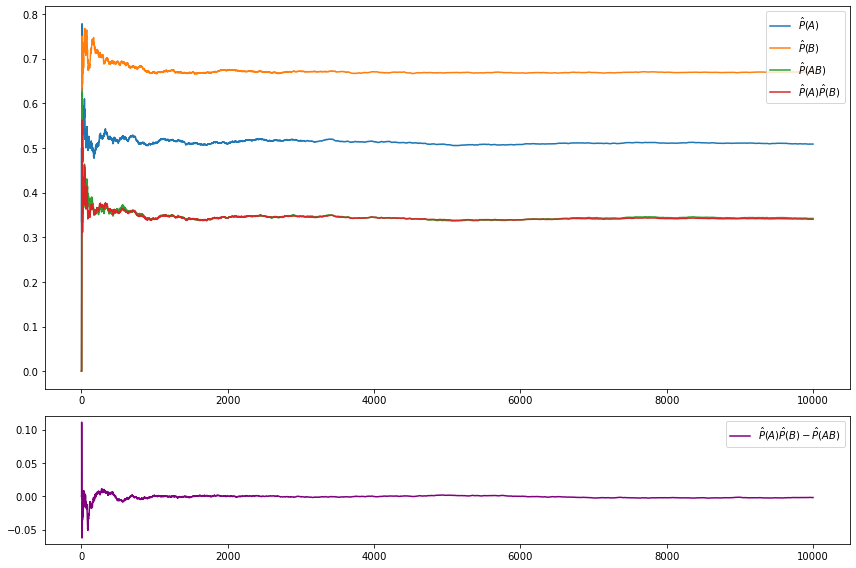
\includegraphics{Figure-02-03}
\end{figure}

\textbf{(b)}
\(\PROB(X > 0) = 1\), so \(\PROB(Y > 0) = 1\). For \(y > 0\),
we have:
\[
F_Y(y) = \PROB(Y \leq y) 
= \PROB\left(\frac{1}{X} \leq y\right) 
= \PROB\left(X \geq \frac{1}{y}\right) 
= 1 - F_X\left(\frac{1}{y} \right)
\]
so
\[
F_Y(y) = 
\begin{cases}
0 
&\text{if } y \leq \Frac{1}{5} \\
\Frac{15}{8} - \frac{3}{8y} 
&\text{if } \frac{1}{5} < y \leq \frac{1}{3} \\
\Frac{3}{4} 
&\text{if } \frac{1}{3} < y \leq 1 \\
1 - \Frac{1}{4y} 
&\text{if } y > 1
\end{cases}
\]

\begin{python}
import numpy as np
import matplotlib.pyplot as plt
plt.figure(figsize=(12, 8))
# Draw horizontal lines
for xmin, xmax, y in [(-2, 1/5, 0), (1/3, 1, 3/4)]:
    plt.hlines(y, xmin, xmax, color='C0')
    
# Draw increasing segments
yy = np.arange(1/5, 1/3, step=0.001)
plt.plot(yy, 15/8 - 3/(8 * yy), color='C0')
yy = np.arange(1, 8, step=0.01)
plt.plot(yy, 1 - 1/(4*yy), color='C0')
    
plt.xlabel(r'$y$')
plt.ylabel(r'$F_Y(y)$')
plt.show()
\end{python}

\begin{figure}[H]
\centering
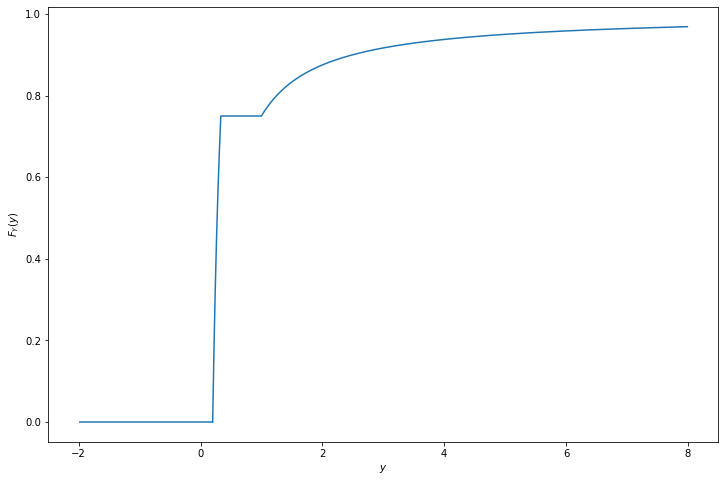
\includegraphics{Figure-03-04}
\end{figure}

The probability density function is \(f_y(y) = F'_Y(y)\), so
\[
f_Y(y) = 
\begin{cases}
0
&\text{if } y \leq \frac{1}{5} \\
\frac{3}{8y^{2}} 
&\text{if } \frac{1}{5} < y \leq \frac{1}{3} \\
0 
&\text{if } \frac{1}{3} < y \leq 1 \\
\frac{1}{4y^{2}} 
&\text{if } y > 1
\end{cases}
\]

\begin{python}
import numpy as np
import matplotlib.pyplot as plt
def f_Y(y):
    return np.where(y <= 1/5, 0, np.where(y <= 1/3, 3/(8 * (y**2)), 
                    np.where(y <= 1, 0, 1/(4 * (y**2)))))
plt.figure(figsize=(12, 8))
yy = np.arange(-1, 3, step=0.001)
plt.plot(yy, f_Y(yy), color='C0')
    
plt.xlabel(r'$y$')
plt.ylabel(r'$f_Y(y)$')
plt.show()
\end{python}

\begin{figure}[H]
\centering
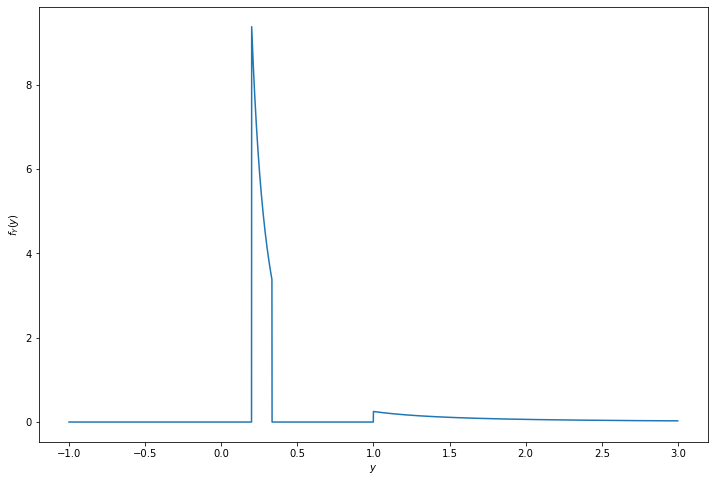
\includegraphics{Figure-03-05}
\end{figure}


\textbf{Exercise 3.14.5}. Let \(X\) and \(Y\) be discrete random
variables. Show that \(X\) and \(Y\) are independent if and only if
\(f_{X, Y}(x, y) = f_X(x) f_Y(y)\) for all \(x\) and \(y\).

\textbf{Solution}. If \(x\) or \(y\) take values that have probability
mass 0, then trivially \(f_{X, Y}(x, y) = 0\) and \(f_X(x) f_Y(y) = 0\),
so we only need to consider \(x\) and \(y\) with positive probability
mass.
If \(X\) and \(Y\) are independent, then
\(\PROB(X \in A, Y \in B) = \PROB(X \in A)\PROB(Y \in B)\)
for all events \(A\), \(B\). In particular, this is true for
\(A = \{x\}\) and \(B = \{ y \}\) for all \(x, y\), proving the
implication in one direction.
In the other direction, we have
\[
\PROB(X \in A, Y \in B) = \sum_{x \in A} \sum_{y \in B} f_{X, Y}(x, y)
\]
and
\[
\PROB(X \in A) = \sum_{x \in A} f_X(x)
\quad \text{and} \quad
\PROB(Y \in B) = \sum_{y \in B} f_Y(y)
\]
so \(f_{X, Y}(x, y) = f_X(x) f_Y(y)\) for all \(x, y\) implies that for
all \(A\) and \(B\),
\begin{align*}
\PROB(X \in A) \PROB(Y \in B) 
& = \left( \sum_{x \in A} f_X(x) \right) \left( \sum_{y \in B} f_Y(y) \right)
\\
& = \sum_{x \in A} \sum_{y \in B} f_X(x) f_Y(y) 
\\
& = \sum_{x \in A} \sum_{y \in B} f_{X, Y}(x, y) = \PROB(X \in A, Y \in B)
\end{align*}
so \(X, Y\) are independent, proving the implication in the other
direction.

\textbf{Exercise 3.14.6}. Let \(X\) have distribution \(F\) and density
function \(f\) and let \(A\) be a subset of the real line. Let
\(I_A(x)\) be the indicator function for \(A\):
\[
I_A(x) = \begin{cases}
1 &\text{if } x \in A 
\\[
1ex]
0 &\text{otherwise}
\end{cases}
\]
Let \(Y = I_A(X)\). Find an expression for the cumulative distribution
function of \(Y\). (Hint: first find the mass function for \(Y\).)

\textbf{Solution}. Note that \(I_A\) can only return values 0 or 1, so
\(Y\) is a discrete variable with non-zero probability mass only at
values 0 and 1.
But $\PROB(Y = 1) = \PROB(x \in A) = \int\_A f\_X(x) dx $,
so the PDF for \(Y\) is:
\[
f_Y(y) = \begin{cases}
\int_A f_X(x) dx &\text{if } y = 1 \\
1 - \int_A f_X(x) dx &\text{if } y = 0 \\
0 &\text{otherwise}
\end{cases}
\]
and so the CDF of \(Y\) is:
\[
F_Y(y) = \begin{cases}
0 &\text{if } y < 0 \\
1 - \int_A f_X(x) dx &\text{if } 0 \leq y < 1 \\
1 &\text{if } y \geq 1
\end{cases}
\]

\textbf{Exercise 3.14.7}. Let \(X\) and \(Y\) be independent and suppose
that each has a \(\text{Uniform}(0, 1)\) distribution. Let
\(Z = \min \{ X, Y \}\). Find the density \(f_Z(z)\) for \(Z\). Hint: it
might be easier to first find \(\PROB(Z > z)\).

\textbf{Solution}.
\[
1 - F_Z(z) = \PROB(Z > z) = \PROB(X > z, Y > z) = (1 - F_X(z)) (1 - F_Y(z))
\]
But \(F_X\) and \(F_Y\) are both the CDF of the \(\text{Uniform}(0, 1)\)
distribution, so
\[
F_X(x) = \begin{cases}
0 &\text{if } x \leq 0 \\
x &\text{if } 0 < x \leq 1 \\
1 &\text{if } x > 1
\end{cases}
\]
and so
\[
F_Z(z) = \begin{cases}
0 &\text{if } z \leq 0 \\
2z - z^{2} &\text{if } 0 < z \leq 1 \\
1 &\text{if } z > 1
\end{cases}
\]
and the PDF is \(f_Z(z) = F'_Z(z)\):
\[
f_Z(z) = \begin{cases}
0 &\text{if } z \leq 0 \\
2 - 2z &\text{if } 0 < z < 1 \\
0 &\text{if } z > 1
\end{cases}
\]

\begin{python}
import numpy as np
import matplotlib.pyplot as plt
def f_Z(z):
    return np.where(z <= 0, 0, np.where(z >= 1, 0, 2 - 2 * z))
plt.figure(figsize=(12, 8))
zz = np.arange(-0.5, 1.5, step=0.01)
plt.plot(zz, f_Z(zz), color='C0')
    
plt.xlabel(r'$z$')
plt.ylabel(r'$f_Z(z)$')
plt.show()
\end{python}

\begin{figure}[H]
\centering
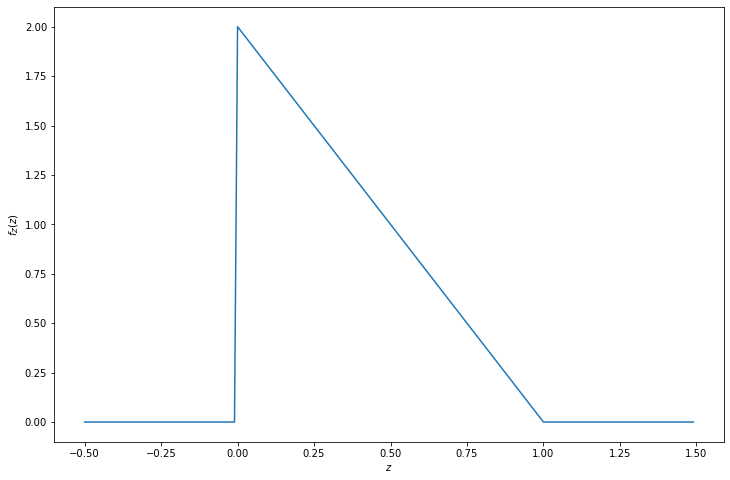
\includegraphics{Figure-03-06}
\end{figure}


\textbf{Exercise 3.14.8}. Let \(X\) have CDF \(F\). Find the CDF of
\(X^+ = \max \{0, X\}\).

\textbf{Solution}.
\[
F_{X^+}(x) = \PROB(X^+ \leq x) = \PROB(0 < x, X < x) = I(0 < x) F_X(x)
\]

\textbf{Exercise 3.14.9}. Let \(X \sim \text{Exp}(\beta)\). Find
\(F(x)\) and \(F^{-1}(q)\).

\textbf{Solution}. Start from the definition for the PDF of the
exponential distribution:
\[
f(x) = \frac{1}{\beta} e^{-x / \beta}, \quad x > 0
\]
We have:
\[
F(x) = \int_{-\infty}^x f(t) dt = \int_{-\infty}^x \frac{1}{\beta} e^{-t / \beta} dt = \frac{1}{\beta} \beta \left( 1 - e^{-x / \beta} \right) = 1 - e^{-x / \beta}
\]
and so
\[
q = 1 - e^{-F^{-1}(q) / \beta} \Longrightarrow F^{-1}(q) = -\beta \log (1 - q)
\]

\textbf{Exercise 3.14.10}. Let \(X\) and \(Y\) be independent. Show that
\(g(X)\) is independent of \(h(Y)\) where \(g\) and \(h\) are functions.

\textbf{Solution}. Let \(g^{-1}(A) = \{ x : g(x) \in A \}\) and
\(h^{-1}(B) = \{ y : h(y) \in B \}\). We have:
\begin{align*}
\PROB(g(X) \in A, h(Y) \in B) 
& = \PROB(X \in g^{-1}(A), Y \in h^{-1}(B) 
\\
& = \PROB(X \in g^{-1}(A)) \PROB(Y \in h^{-1}(B)) 
\\
& = \PROB(g(X) \in A) \PROB(h(Y) \in B)
\end{align*}

\textbf{Exercise 34.14.11}. Suppose we toss a coin once and let \(p\) be
the probability of heads. Let \(X\) denote the number of heads and \(Y\)
denote the number of tails.
\textbf{(a)} Prove that \(X\) and \(Y\) are dependent.
\textbf{(b)} Let \(N \sim \text{Poisson}(\lambda)\) and suppose that we
toss a coin \(N\) times. Let \(X\) and \(Y\) be the number of heads and
tails. Show that \(X\) and \(Y\) are independent.

\textbf{Solution}.
\textbf{(a)} The joint probability mass function is:
\[
\begin{array}{c|cc}
f_{X, Y} & Y = 0 & Y = 1 \\
\hline
X = 0 & 0 & 1 - p\\
X = 1 & p & 0
\end{array}
\]
In particular, \(f_{X, Y}(1, 0) = p\) and \(f_X(1) f_Y(0) = p^{2}\), so
the events are dependent unless \(p \in \{0, 1\}\).
\textbf{(b)} The joint probability mass function is:
\begin{align*}
\PROB(X = x, Y = y) 
  = \PROB(N = x + y, X = x) 
& = \frac{\lambda^{x+y}e^{-\lambda}}{(x + y)!} \binom{x + y}{x} p^x (1-p)^y 
\\[
1ex]
& = e^{-\lambda} \left(\frac{\lambda^x}{x!} p^x \right) \left(\frac{\lambda^y}{y!} (1 - p)^y\right) 
  = g(x) h(y)
\end{align*}
where \(g(x) =  \frac{e^{-\lambda}\lambda^x}{x!} p^{x}\), 
\(h(y) = \frac{\lambda^y}{y!} (1 - p)^{y} \). 
The result then follows from Theorem 3.33.

\textbf{Exercise 3.14.12}. Prove Theorem 3.33.
Suppose that the range of \(X\) and \(Y\) is a (possibly infinite)
rectangle. If \(f(x, y) = g(x) h(y)\) for some functions \(g\) and \(h\)
(not necessarily probability density functions) then \(X\) and \(Y\) are
independent.

\textbf{Solution}.
Given that \(F\) is the joint probability density function of \(X\) and
\(Y\), then the marginal distributions for \(X\) and \(Y\) are
\[
f_X(x) = \int f(x, y) dy = \int g(x) h(y) dy = g(x) \int h(y) dy = H g(x) \quad \text{ for some constant } H
\]
and
\[
f_Y(y) = \int f(x, y) dx = \int g(x) h(y) dx = h(y) \int g(x) dx = G h(y) \quad \text{ for some constant } G
\]
Therefore,
\[
f_X(x) f_Y(y) = HG g(x) h(y) = HG f(x, y)
\]
Integrating over \(x\), and fixing \(y = y_{0}\) with non-zero probability
density,
\[
\int f_X(x) f_Y(y_{0}) dx = HG \int f(x, y_{0}) dx \Longrightarrow f_Y(y_{0}) = HG f_Y(y_{0}) \Longrightarrow HG = 1
\]
and so
\[
f_X(x) f_Y(y) = f(x, y)
\]
therefore \(X\) and \(Y\) are independent.

\textbf{Exercise 3.14.13}. Let \(X \sim N(0, 1)\) and let \(Y = e^X\).
\textbf{(a)} Find the PDF for \(Y\). Plot it.
\textbf{(b) (Computer Experiment)} Generate a vector
\(x = (x_{1}, \dots, x_{10,000})\) consisting of 10,000 random standard
Normals. Let \(y = (y_{1}, \dots, y_{10,000})\) where \(y_{i} = e^{x_{i}}\).
Draw a histogram of \(y\) and compare it to the PDF you found in part
(a).

\textbf{Solution}.
\textbf{(a)}
Assuming \(y > 0\),
\[
F_Y(y) = \PROB(Y \leq y) = \PROB(X \leq \log y) = \Phi(\log y)
\]
and so
\[
f_Y(y) = \frac{d}{dy} \Phi(\log y) = \frac{d \Phi(\log y)}{d \log y} \frac{d \log y}{dy} = \frac{\phi(\log(y))}{y}
\]
And, of course, \(Y\) can never take a negative value, so
\[
f_Y(y) =
\begin{cases}
\frac{\phi(\log(y))}{y} &\text{if } y > 0 
\\[
1ex]
0 &\text{otherwise}
\end{cases}
\]

\begin{python}
import numpy as np
from scipy.stats import norm
import matplotlib.pyplot as plt
yy = np.arange(0.01, 5, step=0.01)
def f_Y(y):
    return norm.pdf(np.log(y)) / y
plt.figure(figsize=(12, 8))
plt.plot(yy, f_Y(yy))
plt.xlabel(r'$y$')
plt.ylabel(r'$f_Y(y)$')
plt.show()
\end{python}

\begin{figure}[H]
\centering
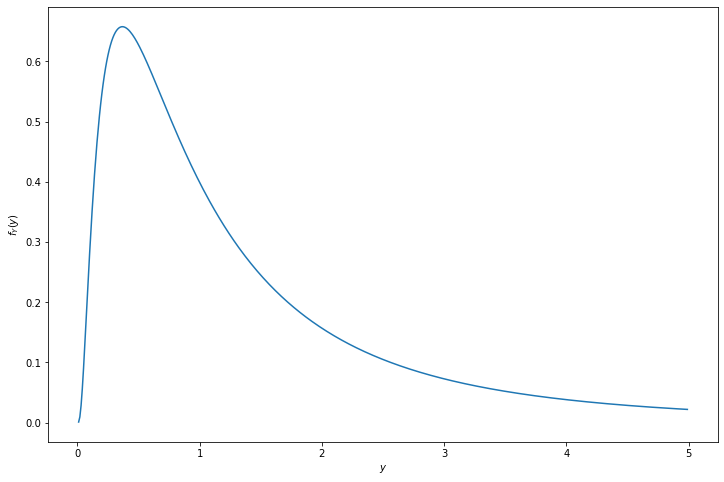
\includegraphics{Figure-03-07}
\end{figure}

\textbf{(b)}

\begin{python}
np.random.seed(0)
N = 10000
X = norm.rvs(size=N)
Y = np.exp(X)
plt.figure(figsize=(12, 8))
plt.hist(Y, bins=200, density=True, label='histogram', histtype='step')
plt.plot(yy, f_Y(yy), label='true density')
plt.legend(loc='upper right')
plt.xlim(0, 5)
plt.show()
\end{python}

\begin{figure}[H]
\centering
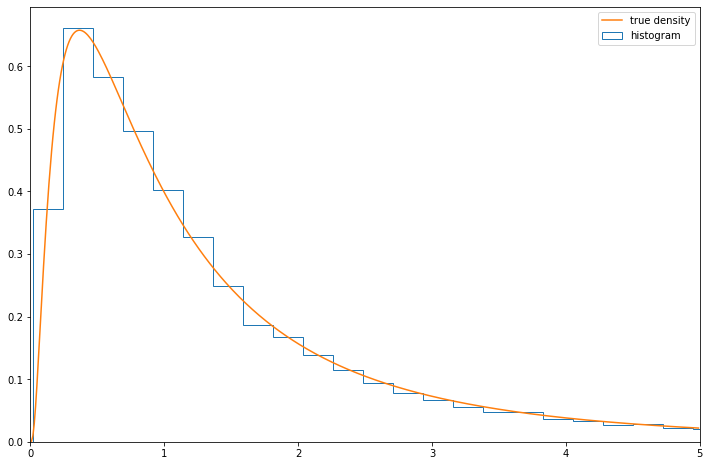
\includegraphics{Figure-03-08}
\end{figure}


\textbf{Exercise 3.14.14}. Let \((X, Y)\) be uniformly distributed on
the unit disc \(\{ (x, y) : x^{2} + y^{2} \leq 1 \}\). Let
\(R = \sqrt{X^{2} + Y^{2}}\). Find the CDF and the PDF of \(R\).

\textbf{Solution}.
Assuming \(r > 0\),
\[
F_R(r) = \PROB(R \leq r) = \PROB(X^{2} + Y^{2} \leq r^{2}) = \int \int_{x^{2} + y^{2} \leq r^{2}} f(x, y) dx dy
\]
is proportional to the area of a disc of radius \(r\). Since
\(F_R(1) = 1\), we have that the CDF is
\[
F_R(r) = \begin{cases}
0 &\text{if } r \leq 0 \\
r^{2} &\text{if } 0 < r \leq 1 \\
1 &\text{if } r > 1
\end{cases}
\]
and the PDF is \(f_R(r) = F'_R(r)\):
\[
f_R(r) = \begin{cases}
0 &\text{if } r \leq 0 \\
2 r &\text{if } 0 < r \leq 1 \\
0 &\text{if } r > 1
\end{cases}
\]

\textbf{Exercise 3.14.15 (A universal random number generator)}. Let
\(X\) have a continuous, strictly increasing CDF. Let \(Y = F(X)\). Find
the density of \(Y\). This is called the probability integral
transformation. Now let \(U \sim \text{Uniform}(0, 1)\) and let
\(X = F^{-1}(U)\). Show that \(X \sim F\). Now write a program that
takes \(\text{Uniform}(0, 1)\) random variables and generates random
variables from a \(\text{Exp}(\beta)\) distribution.

\textbf{Solution}.
For \(0 \leq y \leq 1\), the CDF of \(Y\) is
\[
F_Y(y) = \PROB(Y \leq y) = \PROB(F(X) \leq y) = \PROB(X \leq F^{-1}(y)) = F(F^{-1}(y)) = y
\]
and so \(Y \sim \text{Uniform}(0, 1)\).
For \(0 \leq q \leq 1\),
\[
F_X(q) = \PROB(X \leq q) = \PROB(F(X) \leq F(q)) = \PROB(U \leq F(q)) = F(q)
\]
and so \(X \sim F\).
To create a generator for \(\text{Exp}(\beta)\), let \(F\) be the CDF
for this distribution,
\[
F(x) = 1 - e^{-x/\beta} \quad F^{-1}(q) = - \beta \log (1 - q)
\]

\begin{python}
import numpy as np
def inv_F(beta):
    def inv_f_impl(q):
        return -beta * np.log(1 - q)
    return inv_f_impl
\end{python}

\begin{python}
np.random.seed(0)
N = 100000
U = np.random.uniform(low=0, high=1, size=N)
X = {}
for beta in [0.1, 1.0, 10.0]:
    X[beta] = inv_F(beta)(U)
\end{python}

\begin{python}
import matplotlib.pyplot as plt
from scipy.stats import expon
plt.figure(figsize=(12, 8))
for i, beta in enumerate([0.1, 1.0, 10]):
    ax = plt.subplot(3, 1, (i + 1))
    ax.hist(X[beta], density=True, bins=100, histtype='step', label='simulation histogram')
    xx = np.arange(beta * 0.01, 5 * beta, step=beta * 0.01)
    ax.plot(xx, expon.pdf(xx, scale=beta), label='true PDF')
    ax.set_xlim(-beta * 0.1, 5 * beta)
    ax.legend(loc='upper right')
    ax.set_title('beta = ' + str(beta))
    
plt.tight_layout()
plt.show()
\end{python}

\begin{figure}[H]
\centering
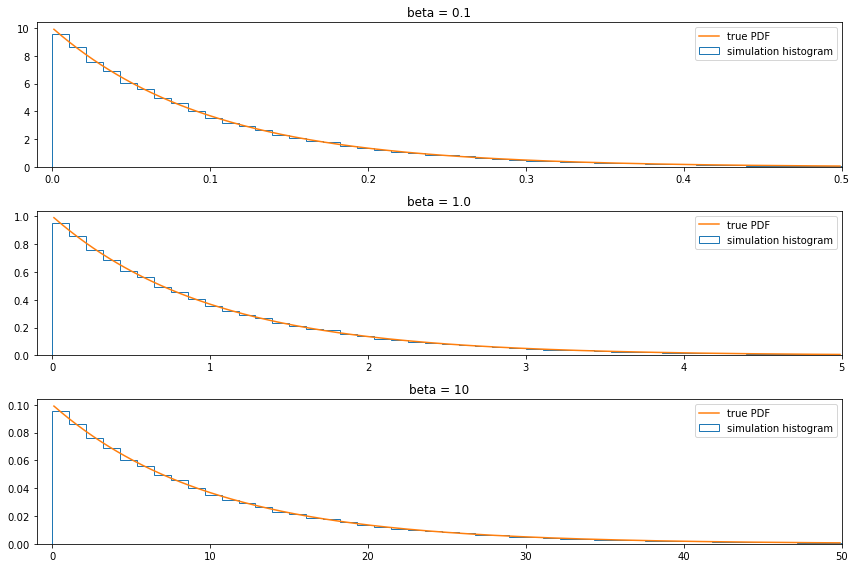
\includegraphics{Figure-03-09}
\end{figure}


\textbf{Exercise 3.14.16}. Let \(X \sim \text{Poisson}(\lambda)\) and
\(Y \sim \text{Poisson}(\mu)\) and assume that \(X\) and \(Y\) are
independent. Show that the distribution of \(X\) given that
\(X + Y = n\) is \(\text{Binomial}(n, \pi)\) where
\(\pi = \lambda / (\lambda + \mu)\).
Hint 1: You may use the following fact: If
\(X \sim \text{Poisson}(\lambda)\) and \(Y \sim \text{Poisson}(\mu)\),
and \(X\) and \(Y\) are independent, then
\(X + Y \sim \text{Poisson}(\mu + \lambda)\).
Hint 2: Note that \(\{X = x, X + Y = n\} = \{X = x, Y = n - x \}\)

\textbf{Solution}.
We have:
\begin{align*}
\PROB(X = x | X + Y = n) &= \frac{\PROB(X = x, X + Y = n)}{\PROB(X + Y = n)} \\
&= \frac{\PROB(X = x, Y = n - x)}{\PROB(X + Y = n)} \\
&= \frac{\PROB(X = x) \PROB(Y = n - x)}{\PROB(X + Y = n)} \\
&= \frac{\frac{\lambda^x e^{-\lambda}}{x!} \frac{\mu^{n - x} e^{-\mu}}{(n - x)!} }{\frac{(\lambda + \mu)^{n} e^{-(\lambda + \mu)}}{n!}} \\
&= \frac{n!}{x! (n - x)!} \frac{\lambda^x \mu^{n - x}}{(\lambda + \mu)^{n}} \\
&= \binom{n}{x} \left( \frac{\lambda}{\lambda + \mu} \right)^x \left( \frac{\mu}{\lambda + \mu}\right)^{n - x} \\
&= \binom{n}{x} \pi^x (1 - \pi)^{n - x}
\end{align*}
and so the result follows.

\textbf{Exercise 3.14.17}. Let
\[
f_{X, Y}(x, y) = 
\begin{cases}
c(x + y^{2}) &\text{if } 0 \leq x \leq 1 \text{ and }  0 \leq y \leq 1 
\\[
1ex]
0 & \text{otherwise}
\end{cases}
\]
Find \(\PROB\left( X < \frac{1}{2} | Y = \frac{1}{2} \right)\).

\textbf{Solution}.
The conditional density \(f_{X | Y}(x | y)\) is:
\[
f_{X|Y}(x | y) = \frac{f_{X, Y}(x, y)}{f_Y(y)} = \frac{f_{X, Y}(x, y)}{\int f_{X, Y}(t, y) dt}
= \frac{ c(x + y^{2}) }{\int_{0}^{1} c(t + y^{2}) dt} =  \frac{ x + y^{2} }{\int_{0}^{1} t + y^{2} dt} = \frac{x + y^{2}}{\frac{1}{2} + y^{2}}
\]
In particular, when \(y = 1/2\),
\[
f_{X|Y}(x | 1/2) = \frac{4x + 1}{3}
\]
and so
\[
\PROB\left( X < x \;\Bigg|\; Y = \frac{1}{2} \right) = \int_{0}^x \frac{4t + 1}{3} dt = \frac{2x^{2} + x}{3}
\]
so
\[
\PROB\left( X < \frac{1}{2} \;\Bigg|\; Y = \frac{1}{2} \right) = \frac{1}{3}
\]
\textbf{Exercie 3.14.18}. Let \(X \sim N(3, 16)\). Solve the following
using the Normal table and using a computer package.
\textbf{(a)} Find \(\PROB(X < 7)\).
\textbf{(b)} Find \(\PROB(X > -2)\).
\textbf{(c)} Find \(x\) such that \(\PROB(X > x) = .05\).
\textbf{(d)} Find \(\PROB(0 \leq X < 4)\).
\textbf{(e)} Find \(x\) such that \(\PROB(|X| > |x|) = .05\).

\textbf{Solution}.
Rather than using tables, we will express these in terms of a standard
Normal, and use ``computer packages'' to compute the expression based
both on the original Normal and the standard Normal.
\textbf{(a)}
\(\PROB(X < 7) = \PROB\left(\frac{X - 3}{4} < \frac{7 - 3}{4} \right) = \PROB\left(Z < 1 \right) = \Phi\left( 1 \right)\)

\begin{python}
import numpy as np
from scipy.stats import norm
print('%.4f' % norm.cdf(1))
print('%.4f' % norm.cdf(7, loc=3, scale=4))
\end{python}
\begin{console}
0.8413
0.8413
\end{console}
\textbf{(b)} $\PROB(X > -2) =
\PROB\left(\frac{X - 3}{4} > \frac{-2 - 3}{4} \right)
= \PROB\left(Z < -\frac{5}{4} \right) = 1 - \Phi\left(
-\frac{5}{4} \right) $

\begin{python}
import numpy as np
from scipy.stats import norm
print('%.4f' % (1 - norm.cdf(-5/4)))
print('%.4f' % (1 - norm.cdf(-2, loc=3, scale=4)))
\end{python}
\begin{console}
0.8944
0.8944
\end{console}
\textbf{(c)} \(\PROB(X > x) = .05
\Longleftrightarrow 1 - F_X(x) = .05
\Longleftrightarrow F_X(x) = .95
\Longleftrightarrow x = F_X^{-1}(.95)\)
or: \(\PROB(X > x) = .05
\Longleftrightarrow \PROB\left(\frac{X - 3}{4} > \frac{x - 3}{4}\right) = .05
\Longleftrightarrow 1 - \Phi\left(\frac{x - 3}{4}\right) = .05
\Longleftrightarrow \frac{x - 3}{4} = \Phi^{-1}(.95)
\Longleftrightarrow x = 4 \Phi^{-1}(.95) + 3\)

\begin{python}
import numpy as np
from scipy.stats import norm
print('%.4f' % norm.ppf(.95, loc=3, scale=4))
print('%.4f' % (4 * norm.ppf(.95) + 3))
\end{python}
\begin{console}
9.5794
9.5794
\end{console}
\textbf{(d)} \(\PROB(0 \leq X < 4) = F_X(4) - F_X(0)\)
or
\(\PROB(0 \leq X < 4) = \PROB\left(\frac{0 - 3}{4} < Z < \frac{4 - 3}{4} \right) = \Phi\left( \frac{1}{4} \right) - \Phi\left( \frac{-3}{4} \right)\)

\begin{python}
import numpy as np
from scipy.stats import norm
print('%.4f' % (norm.cdf(4, loc=3, scale=4) - norm.cdf(0, loc=3, scale=4)))
print('%.4f' % (norm.cdf(1/4) - norm.cdf(-3/4)))
\end{python}
\begin{console}
0.3721
0.3721
\end{console}
\textbf{(e)} \(\PROB(|X| > |x|) = .05\)
For a constant \(c \geq 0\), we have
\begin{align*}
\PROB(|X| > c) &= 1 - \PROB(|X| < c) = 1 - \PROB(-c < X < -c) \\
&= 1 - \PROB\left( -\frac{c - 3}{4} < Z < \frac{c - 3}{4} \right)\\
&= 1 - \Phi\left( \frac{c - 3}{4} \right) + \Phi\left( -\frac{c - 3}{4} \right) \\
&= 2 - 2 \Phi\left( \frac{c - 3}{4} \right) = 2 - 2 F_X(c)
\end{align*}
So we can solve the original equation:
\[
2 - 2 F_X(c) = .05 \Longleftrightarrow c = F_X^{-1}(0.975)
\]
or
\[
2 - 2 \Phi\left( \frac{c - 3}{4} \right) = .05 \Longleftrightarrow c = 4 \Phi^{-1}(0.975) + 3
\]

\begin{python}
import numpy as np
from scipy.stats import norm
print('%.4f' % (norm.ppf(0.975, loc=3, scale=4)))
print('%.4f' % (4 * norm.ppf(0.975) + 3))
\end{python}
\begin{console}
10.8399
10.8399
\end{console}

\textbf{Exercise 3.14.19}. Prove formula (3.11).
Given \(Y = r(X)\), when \(r\) is strictly monotone increasing or
strictly monotone decreasing then \(r\) has an inverse \(s = r^{-1}\)
and in this case one can show that
\[
f_Y(y) = f_X(s(y)) \;\Bigg| \frac{ds(y)}{dy} \Bigg|
\]

\textbf{Solution}.
Assume \(r\) is strictly monotone increasing. Then $ \frac{d s(y)}{dy}
> 0$, and the CDF of \(Y\) is
\[
F_Y(y) = \PROB(Y \leq y) = \PROB(r(X) \leq y) = \PROB(X \leq s(y)) = F_X(s(y))
\]
Derivating over \(y\),
\begin{align*}
\frac{d}{dy} F_y(y) &= \frac{d F_X(s(y))}{d s(y)} \frac{d s(y)}{dy} \\
f_Y(y) &= f_X(s(y)) \frac{d s(y)}{dy}
\end{align*}
For the case when \(r\) is strictly monotone decreasing, $
\frac{d s(y)}{dy} < 0$, and the CDF of \(Y\) is
\[
F_Y(y) = \PROB(Y \leq y) = \PROB(r(X) \leq y) = \PROB(X \geq s(y)) = 1 - F_X(s(y))
\]
Derivating over \(y\),
\begin{align*}
\frac{d}{dy} F_y(y) &= \frac{d -F_X(s(y))}{d s(y)} \frac{d s(y)}{dy} \\
f_Y(y) &= -f_X(s(y)) \frac{d s(y)}{dy}
\end{align*}
and the result follows.

\textbf{Exercise 3.14.20}. Let \(X, Y \sim \text{Uniform}(0, 1)\) be
independent. Find the PDF for \(X - Y\) and \(X / Y\).

\textbf{Solution}.
The joint density of \(X, Y\) is
\[
f(x, y) = 
\begin{cases}
1 &\text{if } 0 \leq x \leq 1, 0 \leq y \leq 1 
\\[
1ex]
0 &\text{otherwise}
\end{cases}
\]
Let \(A = X - Y\). The CDF of \(A\) is calculated over the area
\(A_a = \{ (x, y) : x - y \leq a \}\):
\[
F_A(a) = \PROB(X + Y \leq a) = \int_{A_a} f(x, y)\; dx dy
\]
\begin{itemize}
\item
  If \(0 \leq a \leq 1\), the area is consists of all points in the unit
  square, othe than the triangle at points
  \((a, 0), (1, 0), (1, 1 - a)\). Then,
  \[
F_A(a) = 1 - \frac{(1 - a)^{2}}{2}
\]
\item
  If \(-1 \leq a \leq 0\), the area consists of only the points in the
  triangle \((0, 1), (1 + a, 1), (0, -a)\). Then,
  \[
F_A(a) = \frac{(1 + a)^{2}}{2}
\]
\end{itemize}
Therefore, the PDF is \(f_A(a) = F'_A(a)\), or
\[
f_A(a) =
\begin{cases}
1 + a &\text{if } -1 < a \leq 0
\\[
1ex]
1 - a &\text{if } 0 < a \leq 1
\\[
1ex]
0 &\text{otherwise}
\end{cases} 
\]

\begin{python}
import numpy as np
import matplotlib.pyplot as plt
plt.figure(figsize=(8, 4))
ax = plt.subplot(1, 2, 1)
a = 1/3
x = [0, a, 1, 1, 0]
y = [0, 0, 1 - a, 1, 1]
ax.fill(x, y)
ax.set_xlim(-0.5, 1.5)
ax.set_ylim(-0.5, 1.5)
ax.set_title('a = 1/3')
ax = plt.subplot(1, 2, 2)
a = -1/3
x = [0, 1+a, 0]
y = [1, 1, -a]
ax.fill(x, y)
ax.set_xlim(-0.5, 1.5)
ax.set_ylim(-0.5, 1.5)
ax.set_title('a = -1/3')
plt.tight_layout()
plt.show()
\end{python}

\begin{figure}[H]
\centering
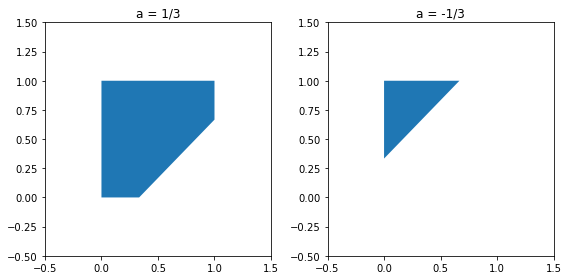
\includegraphics{Figure-03-10}
\end{figure}

Let \(B = X/Y\). The CDF of \(B\) is calculated over the area
\(B_b = \left\{ (x, y) : \frac{x}{y} \leq b \right\}\).
\[
F_B(a) = \PROB\left(\frac{X}{Y} \leq b\right) = \int_{B_b} f(x, y)\; dx dy
\]
\begin{itemize}
\item
  If \(0 < b \leq 1\), the relevant area is a triangle with points
  \((0, 0), (1, 0), (1, b)\). Then,
  \[
F_B(b) = \frac{b}{2}
\]
\item
  If \(b > 1\), the relevant area is the unit square minus the triangle
  with points \((0, 0), (0, 1), (1/b, 1)\). Then,
  \[
F_B(b) = 1 - \frac{1}{2b}
\]
\end{itemize}
Therefore, the PDF is \(f_B(b) = F'_B(b)\), or
\[
f_A(a) =
\begin{cases}
\frac{1}{2} &\text{if } 0 < b \leq 1
\\[
1ex]
\frac{1}{2b^{2}} &\text{if } b > 1
\\[
1ex]
0 &\text{otherwise}
\end{cases}
\]

\begin{python}
import numpy as np
import matplotlib.pyplot as plt
plt.figure(figsize=(8, 4))
ax = plt.subplot(1, 2, 1)
b = 1/3
x = [0, b, 0]
y = [0, 1, 1]
ax.fill(x, y)
ax.set_xlim(-0.5, 1.5)
ax.set_ylim(-0.5, 1.5)
ax.set_title('b = 1/3')
ax = plt.subplot(1, 2, 2)
b = 3
x = [0, 1, 1, 0]
y = [0, 1/b, 1, 1]
ax.fill(x, y)
ax.set_xlim(-0.5, 1.5)
ax.set_ylim(-0.5, 1.5)
ax.set_title('b = 3')
plt.tight_layout()
plt.show()
\end{python}

\begin{figure}[H]
\centering
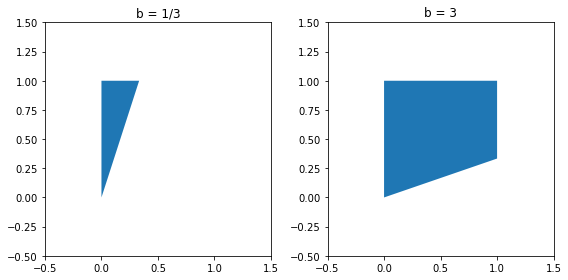
\includegraphics{Figure-03-11}
\end{figure}


\textbf{Exercise 3.14.21}. Let
\(X_{1}, \dots, X_{n} \sim \text{Exp}(\beta)\) be IID. Let
\(Y = \max \{ X_{1}, \dots, X_{n} \}\). Find the PDF of \(Y\). Hint:
\(Y \leq y\) if and only if \(X_{i} \leq y\) for \(i = 1, \dots, n\).

\textbf{Solution}. We have:
\[
\PROB(Y \leq y) = \PROB(\forall i, X_{i} \leq y) = \prod_{i} \PROB(X_{i} \leq y) = \prod_{i} \left(1 - e^{-y/\beta}\right) = (1 - e^{-y/\beta})^{n}
\]
and so the PDF is \(f_Y(y) = F'_Y(y)\):
\[
f_Y(y) = \frac{d (1 - e^{-y/\beta})^{n}}{dy} = \frac{n}{\beta} e^{-y/\beta} (1 - e^{-y/\beta})^{n-1}
\]

\textbf{Exercise 3.14.22}. Let \(X\) and \(Y\) be random variables.
Suppose that \(\EXP(Y | X) = X\). Show that
\(\COV(X, Y) = \VAR(X)\).

\textbf{Solution}.
The covariance is:
\[
\COV(X, Y) = \EXP(XY) - \EXP(X) \EXP(Y)
\]
and the variance is
\[
\VAR(X) = \EXP(X^{2}) - \EXP(X)^{2}
\]
We aim to prove that both of those expressions have the same value when
\(\EXP(Y | X) = X\).
Taking the expectaion on \(\EXP(Y | X)\) we get:
\[
\EXP(\EXP(Y | X)) = \int \EXP(Y = y | X) f_Y(y) \; dy = \int y f_Y(y) = \EXP(Y)
\]
so taking the expectation on both sides of \(\EXP(Y | X) = X\)
gives us \(\EXP(Y) = \EXP(X)\).
Now, we have
\begin{align*}
\EXP(XY) &= \int \EXP(XY | X = x) f_X(x) dx \\
&= \int \EXP(xY | X = x) f_X(x) dx \\
&= \int x \EXP(Y | X = x) f_X(x) dx \\
&= \int x^{2} f_X(x) dx \\
&= \EXP(X^{2})
\end{align*}
Using \(\EXP(X^{2}) = \EXP(XY)\) and
\(\EXP(Y) = \EXP(X)\), we get the desired result.

\textbf{Exercise 3.14.23}. Let \(X \sim \text{Uniform}(0, 1)\). Let
\(0 < a < b < 1\). Let
\[
Y =
\begin{cases}
1 &\text{if } 0 < x < b
\\[
1ex]
0 &\text{otherwise}
\end{cases}
\]
and let
\[
Z =
\begin{cases}
1 &\text{if } a < x < 1 
\\[
1ex]
0 &\text{otherwise}
\end{cases}
\]
\textbf{(a)} Are \(Y\) and \(Z\) independent? Why / Why not?
\textbf{(b)} Find \(\EXP(Y | Z)\). Hint: what values \(z\) can
\(Z\) take? Now find \(\EXP(Y | Z = z)\).

\textbf{Solution}.
\textbf{(a)} The joint probability mass function for \(Y\) and \(Z\) is:
\[
\begin{array}{c|cc}
 & Z = 0 & Z = 1 \\
\hline
Y = 0 & 0 & 1 - b \\
Y = 1 & a & b - a
\end{array}
\]
These are not independent; in particular,
\[
\PROB(Y = 1, Z = 1) = b - a \neq \PROB(Y = 1) \PROB(Z = 1) = b(1 - a)
\]
since the equality would only hold if \(b = 0\) or \(a = 0\), and the
inequality precludes both of these.
\textbf{(b)} We have:
\[
\EXP(Y | Z = 0) = \frac{\sum_y y f(y, 0)}{f_Z(0)} = \frac{f(1, 0)}{a} = 1
\]
and
\[
\EXP(Y | Z = 1) = \frac{\sum_y y f(y, 1)}{f_Z(1)} = \frac{f(1, 1)}{1 - a} = \frac{b - a}{1 - a}
\]


% Chapter 4
\section{4. Expectation}\label{expectation}

\subsection{4.1 Expectation of a Random
Variable}\label{expectation-of-a-random-variable}

The \textbf{expected value}, \textbf{mean} or \textbf{first moment} of
\(X\) is defined to be

\[ \mathbb{E}(X) = \int x \; dF(x) = \begin{cases}
\sum_x x f(x) &\text{if } X \text{ is discrete} \\
\int x f(x)\; dx &\text{if } X \text{ is continuous}
\end{cases} \]

assuming that the sum (or integral) is well-defined. We use the
following notation to denote the expected value of \(X\):

\[ \mathbb{E}(X) = \mathbb{E}X = \int x\; dF(x) = \mu = \mu_X \]

The expectation is a one-number summary of the distribution. Think of
\(\mathbb{E}(X)\) as the average value you'd obtain if you computed the
numeric average \(n^{-1} \sum_{i=1}^n X_i\) for a large number of IID
draws \(X_1, \dots, X_n\). The fact that
\(\mathbb{E}(X) \approx n^{-1} \sum_{i=1}^n X_i\) is a theorem called
the law of large numbers which we will discuss later. We use
\(\int x \; dF(x)\) as a convenient unifying notation between the
discrete case \(\sum_x x f(x)\) and the continuous case
\(\int x f(x) \; dx\) but you should be aware that \(\int x \; dF(x)\)
has a precise meaning discussed in real analysis courses.

To ensure that \(\mathbb{E}(X)\) is well defined, we say that
\(\mathbb{E}(X)\) exists if \(\int_x |x| \; dF_X(x) < \infty\).
Otherwise we say that the expectation does not exist. From now on,
wheneverwe discuss expectations, we implicitly assume they exist.

\textbf{Theorem 4.6 (The rule of the lazy statician)}. Let \(Y = r(X)\).
Then

\[ \mathbb{E}(Y) = \mathbb{E}(r(X)) = \int r(x) \; dF_X(x) \]

As a special case, let \(A\) be an event and let \(r(x) = I_A(x)\),
where \(I_A(x) = 1\) if \(x \in A\) and \(I_A(x) = 0\) otherwise. Then

\[ \mathbb{E}(I_A(X)) = \int I_A(x) f_X(x) dx = \int_A f_X(x) dx = \mathbb{P}(X \in A) \]

In other words, probability is a special case of expectation.

Functions of several variables are handled in a similar way. If
\(Z = r(X, Y)\) then

\[ \mathbb{E}(Z) = \mathbb{E}(r(X, Y)) = \int \int r(x, y) \; dF(x, y) \]

The \textbf{\(k\)-th moment} of \(X\) is defined to be
\(\mathbb{E}(X^k)\), assuming that \(\mathbb{E}(|X|^k) < \infty\). We
shall rarely make much use of moments beyond \(k = 2\).

\subsection{4.2 Properties of
Expectations}\label{properties-of-expectations}

\textbf{Theorem 4.10}. If \(X_1, \dots, X_n\) are random variables and
\(a_1, \dots, a_n\) are constants, then

\[ \mathbb{E}\left( \sum_i a_i X_i \right) = \sum_i a_i \mathbb{E}(X_i) \]

\textbf{Theorem 4.12}. Let \(X_1, \dots, X_n\) be independent random
variables. Then,

\[ \mathbb{E}\left(\prod_i X_i \right) = \prod_i \mathbb{E}(X_i) \]

Notice that the summation rule does not require independence but the
product does.

\subsection{4.3 Variance and
Covariance}\label{variance-and-covariance}

Let \(X\) be a random variable with mean \(\mu\). The \textbf{variance}
of \(X\) -- denoted by \(\sigma^2\) or \(\sigma_X^2\) or
\(\mathbb{V}(X)\) or \(\mathbb{V}X\) -- is defined by

\[ \sigma^2 = \mathbb{E}(X - \mu)^2 = \int (x - \mu)^2\; dF(x) \]

assuming this expectation exists. The \textbf{standard deviation} is
\(\text{sd}(X) = \sqrt{\mathbb{V}(X)}\) and is also denoted by
\(\sigma\) and \(\sigma_X\).

\textbf{Theorem 4.14}. Assuming the variance is well defined, it has the
following properties:

\begin{enumerate}[label={\arabic*.}]
\item
  \(\mathbb{V}(X) = \mathbb{E}(X^2) - \mathbb{E}(X)^2\)
\item
  If \(a\) and \(b\) are constants then
  \(\mathbb{V}(aX + b) = a^2 \mathbb{V}(X)\)
\item
  If \(X_1, \dots, X_n\) are independent and \(a_1, \dots, a_n\) are
  constants then

  \[ \mathbb{V}\left( \sum_{i=1}^n a_iX_i \right) = \sum_{i=1}^n a_i^2 \mathbb{V}(X_i) \]
\end{enumerate}

If \(X_1, \dots, X_n\) are random variables then we define the
\textbf{sample mean} to be

\[ \overline{X}_n = \frac{1}{n} \sum_{i=1}^n X_i  \]

and the \textbf{sample variance} to be

\[ S_n^2 = \frac{1}{n - 1} \sum_{i=1}^n \left(X_i - \overline{X}_n\right)^2 \]

\textbf{Theorem 4.16}. Let \(X_1, \dots, X_n\) be IID and let
\(\mu = \mathbb{E}(X_i)\), \(\sigma^2 = \mathbb{V}(X_i)\). Then

\[ 
\mathbb{E}\left(\overline{X}_n\right) = \mu,
\quad
\mathbb{V}\left(\overline{X}_n\right) = \frac{\sigma^2}{n},
\quad \text{and} \quad
\mathbb{E}\left(S_n^2\right) = \sigma^2
\]

If \(X\) and \(Y\) are random variables, then the covariance and
correlation between \(X\) and \(Y\) measure how strong the linear
relationship between \(X\) and \(Y\) is.

Let \(X\) and \(Y\) be random variables with means \(\mu_X\) and
\(\mu_Y\) and standard deviation \(\sigma_X\) and \(\sigma_Y\). Define
the \textbf{covariance} between \(X\) and \(Y\) by

\[ \text{Cov}(X, Y) = \mathbb{E}[(X - \mu_X)(Y - \mu_Y)] \]

and the \textbf{correlation} by

\[ \rho = \rho_{X, Y} = \rho(X, Y) = \frac{\text{Cov}(X, Y)}{\sigma_X \sigma_Y} \]

\textbf{Theorem 4.18}. The covariance satisfies:

\[ \text{Cov}(X, Y) = \mathbb{E}(XY) - \mathbb{E}(X) \mathbb{E}(Y) \]

The correlation satisfies:

\[ -1 \leq \rho(X, Y) \leq 1 \]

If \(Y = a + bX\) for some constants \(a\) and \(b\) then
\(\rho(X, Y) = 1\) if \(b > 0\) and \(\rho(X, Y) = -1\) if \(b < 0\). If
\(X\) and \(Y\) are independent, then \(\text{Cov}(X, Y) = \rho = 0\).
The converse is not true in general.

\textbf{Theorem 4.19}.

\[ 
\mathbb{V}(X + Y) = \mathbb{V}(X) + \mathbb{V}(Y) + 2 \text{Cov}(X, Y)
\quad \text{ and } \quad
\mathbb{V}(X - Y) = \mathbb{V}(X) + \mathbb{V}(Y) - 2 \text{Cov}(X, Y)
\]

More generally, for random variables \(X_1, \dots, X_n\),

\[ \mathbb{V}\left( \sum_i a_i X_i \right) = \sum_i a_i^2 \mathbb{V}(X_i) + 2 \sum \sum_{i < j} a_i a_j \text{Cov}(X_i, X_j) \]

\subsection{4.4 Expectation and Variance of Important Random
Variables}\label{expectation-and-variance-of-important-random-variables}

\[
\begin{array}{lll}
\text{Distribution} & \text{Mean} & \text{Variance}           \\
\hline
\text{Point mass at } p      & a             & 0              \\
\text{Bernoulli}(p)          & p             & p(1-p)         \\
\text{Binomial}(n, p)        & np            & np(1-p)        \\
\text{Geometric}(p)          & 1/p           & (1 - p)/p^2    \\
\text{Poisson}(\lambda)      & \lambda       & \lambda        \\
\text{Uniform}(a, b)         & (a + b) / 2   & (b - a)^2 / 12 \\
\text{Normal}(\mu, \sigma^2) & \mu           & \sigma^2       \\
\text{Exponential}(\beta)    & \beta         & \beta^2        \\
\text{Gamma}(\alpha, \beta)  & \alpha \beta  & \alpha \beta^2 \\
\text{Beta}(\alpha, \beta)   & \alpha / (\alpha + \beta) & \alpha \beta / ((\alpha + \beta)^2 (\alpha + \beta + 1)) \\
t_\nu                        & 0 \text{ (if } \nu > 1 \text{)} & \nu / (\nu - 2) \text{ (if } \nu > 2 \text{)} \\
\chi^2_p                     & p             & 2p             \\
\text{Multinomial}(n, p)     & np            & \text{see below} \\
\text{Multivariate Nornal}(\mu, \Sigma) & \mu & \Sigma \\
\end{array}
\]

The last two entries in the table are multivariate models which involve
a random vector \(X\) of the form

\[ X = \begin{pmatrix} X_1 \\ \vdots \\ X_k \end{pmatrix} \]

The mean of a random vector \(X\) is defined by

\[ \mu = \begin{pmatrix} \mu_1 \\ \vdots \\ \mu_k \end{pmatrix} = \begin{pmatrix} \mathbb{E}(X_1) \\ \vdots \\ \mathbb{E}(X_k) \end{pmatrix} \]

The \textbf{variance-covariance matrix} \(\Sigma\) is defined to be

\[ \Sigma = \begin{pmatrix}
\mathbb{V}(X_1) & \text{Cov}(X_1, X_2) & \cdots & \text{Cov}(X_1, X_k) \\
\text{Cov}(X_2, X_1) & \mathbb{V}(X_2) & \cdots & \text{Cov}(X_2, X_k) \\
\vdots & \vdots & \ddots & \vdots \\
\text{Cov}(X_k, X_1) & \text{Cov}(X_k, X_2) & \cdots & \mathbb{V}(X_k)
\end{pmatrix} \]

If \(X \sim \text{Multinomial}(n, p)\) then

\[ 
\mathbb{E}(X) = np = n(p_1, \dots, p_k)
\quad \text{and} \quad
\mathbb{V}(X) = \begin{pmatrix}
np_1(1 - p_1) & -np_1p_2 & \cdots & -np_1p_k \\
-np_2p_1 & np_2(1 - p_2) & \cdots & -np_2p_k \\
\vdots & \vdots & \ddots & \vdots \\
-np_kp_1 & -np_kp_2 & \cdots & np_k(1 - p_k)
\end{pmatrix} \]

To see this:

\begin{itemize}[tightlist]
\item
  Note that the marginal distribution of any one component is
  \(X_i \sim \text{Binomial}(n, p_i)\), so \(\mathbb{E}(X_i) = np_i\)
  and \(\mathbb{V}(X_i) = np_i(1 - p_i)\).\\
\item
  Note that, for \(i \neq j\),
  \(X_i + X_j \sim \text{Binomial}(n, p_i + p_j)\), so
  \(\mathbb{V}(X_i + X_j) = n(p_i + p_j)(1 - (p_i + p_j))\).
\item
  Using the formula for the covariance of a sum, for \(i \neq j\),
\end{itemize}

\[ \mathbb{V}(X_i + X_j) = \mathbb{V}(X_i) + \mathbb{V}(X_j) + 2 \text{Cov}(X_i, X_j) =  np_i(1 - p_i) + np_j(1 - p_j) + 2 \text{Cov}(X_i, X_j) \]

Equating the last two formulas we get a formula for the covariance,
\(\text{Cov}(X_i, X_j) = -np_ip_j\).

Finally, here's a lemma that can be useful for finding means and
variances of linear combinations of multivariate random vectors.

\textbf{Lemma 4.20}. If \(a\) is a vector and \(X\) is a random vector
with mean \(\mu\) and variance \(\Sigma\) then

\[ \mathbb{E}(a^T X) = a^T \mu
\quad \text{and} \quad
\mathbb{V}(a^T X) = a^T \Sigma a \]

If \(A\) is a matrix then

\[ \mathbb{E}(A X) = A \mu
\quad \text{and} \quad
\mathbb{V}(AX) = A \Sigma A^T \]

\subsection{4.5 Conditional
Expectation}\label{conditional-expectation}

The conditional expectation of \(X\) given \(Y = y\) is

\[ \mathbb{E}(X | Y = y) = \begin{cases}
\sum x f_{X | Y}(x | y) &\text{ discrete case} \\
\int x f_{X | Y}(x | y) dy &\text{ continuous case}
\end{cases}
\]

If \(r\) is a function of \(x\) and \(y\) then

\[ \mathbb{E}(r(X, Y) | Y = y) = \begin{cases}
\sum r(x, y) f_{X | Y}(x | y) &\text{ discrete case} \\
\int r(x, y) f_{X | Y}(x | y) dy &\text{ continuous case}
\end{cases}
\]

While \(\mathbb{E}(X)\) is a number, \(\mathbb{E}(X | Y = y)\) is a
function of \(y\). Before we observe \(Y\), we don't know the value of
\(\mathbb{E}(X | Y = y)\) so it is a random variable which we denote
\(\mathbb{E}(X | Y)\). In other words, \(\mathbb{E}(X | Y)\) is the
random variable whose value is \(\mathbb{E}(X | Y = y)\) when \(Y\) is
observed as \(y\). Similarly, \(\mathbb{E}(r(X, Y) | Y)\) is the random
variable whose value is \(\mathbb{E}(r(X, Y) | Y = y)\) when \(Y\) is
observed as \(y\).

\textbf{Theorem 4.23 (The rule of iterated expectations)}. For random
variables \(X\) and \(Y\), assuming the expectations exist, we have that

\[ \mathbb{E}[\mathbb{E}(Y | X)] = \mathbb{E}(Y)
\quad \text{and} \quad
\mathbb{E}[\mathbb{E}(X | Y)] = \mathbb{E}(X) \]

More generally, for any function \(r(x, y)\) we have

\[ \mathbb{E}[\mathbb{E}(r(X, Y) | X)] = \mathbb{E}(r(X, Y))
\quad \text{and} \quad
\mathbb{E}[\mathbb{E}(r(X, Y) | Y)] = \mathbb{E}(r(X, Y)) \]

\textbf{Proof}. We will prove the first equation.

\begin{align}
\mathbb{E}[\mathbb{E}(Y | X)] &= \int \mathbb{E}(Y | X = x) f_X(x) dx = \int \int y f(y | x) dy f(x) dx \\
&= \int \int y f(y|x) f(x) dx dy = \int \int y f(x, y) dx dy = \mathbb{E}(Y)
\end{align}

The \textbf{conditional variance} is defined as

\[ \mathbb{V}(Y | X = x) = \int (y - \mu(x))^2 f(y | x) dx \]

where \(\mu(x) = \mathbb{E}(Y | X = x)\).

\textbf{Theorem 4.26}. For random variables \(X\) and \(Y\),

\[ \mathbb{V}(Y) = \mathbb{E}\mathbb{V}(Y | X) + \mathbb{V} \mathbb{E} (Y | X)\]

\subsection{4.6 Technical Appendix}\label{technical-appendix}

\paragraph{4.6.1 Expectation as an
Integral}\label{expectation-as-an-integral}

The integral of a measurable function \(r(x)\) is defined as follows.
First suppose that \(r\) is simple, meaning that it takes finitely many
values \(a_1, \dots, a_k\) over a partition \(A_1, \dots, A_k\). Then
\(\int r(x) dF(x) = \sum_{i=1}^k a_i \mathbb{P}(r(X) \in A_i)\). The
integral of a positive measurable function \(r\) is defined by
\(\int r(x) dF(x) = \lim_i \int r_i(x) dF(x)\), where \(r_i\) is a
sequence of simple functions such that \(r_i(x) \leq r(x)\) and
\(r_i(x) \rightarrow r(x)\) as \(i \rightarrow \infty\). This does not
depend on the particular sequence. The integral of a measurable function
\(r\) is defined to be
\(\int r(x) dF(x) = \int r^+(x) dF(x) - \int r^-(x) dF(x)\) assuming
both integrals are finite, where \(r^+(x) = \max \{ r(x), 0 \}\) and
\(r^-(x) = \min\{ r(x), 0 \}\).

\paragraph{4.6.2 Moment Generating
Functions}\label{moment-generating-functions}

The \textbf{moment generating function (mgf)} or \textbf{Laplace
transform} of \(X\) is defined by

\[ \psi_X(t) = \mathbb{E}(e^{tX}) = \int e^{tx} dF(x) \]

where \(t\) varies over the real numbers.

In what follows, we assume the mgf is well defined for all \(t\) in
small neighborhood of 0. A related function is the characteristic
function, defined by \(\mathbb{E}(e^{itX})\) where \(i = \sqrt{-1}\).
This function is always defined for all \(t\). The mgf is useful for
several reasons. First, it helps us compute the moments of a
distribution. Second, it helps us find the distribution of sums of
random variables. Third, it is used to prove the central limit theorem.

When the mgf is well defined, it can be shown that we can interchange
the operations of differentiation and ``taking expectation''. This leads
to

\[ \psi'(0) = \left[ \frac{d}{dt} \mathbb{E} e^{tX} \right]_{t = 0} = \mathbb{E} \left[ \frac{d}{dt} e^{tX} \right]_{t = 0}
= \mathbb{E}[X e^{tX}]_{t = 0} = \mathbb{E}(X)
\]

By taking further derivatives we conclude that
\(\psi^{(k)}(0) = \mathbb{E}(X^k)\). This gives us a method for
computing the moments of a distribution.

\textbf{Lemma 4.30}. Properties of the mgf.

\begin{enumerate}[tightlist,label={\arabic*.}]
\item
  If \(Y = aX + b\) then \$\psi\_Y(t) = e\^{}\{bt\} \psi\_X(at) \$
\item
  if \(X_1, \dots, X_n\) are independent and \(Y = \sum_i X_i\) then
  \(\psi_Y(t) = \prod_i \psi_{i}(t)\), where \(\psi_i\) is the mgf of
  \(X_i\).
\end{enumerate}

\textbf{Theorem 4.32}. Let \(X\) and \(Y\) be random variables. If
\(\psi_X(t) = \psi_Y(t)\) for all \(t\) in an open interval around 0,
then \(X \overset{d}= Y\).

\textbf{Moment Generating Function for Some Common Distributions}

\[
\begin{array}{ll}
\text{Distribution} & \text{mgf} \\
\hline
\text{Bernoulli}(p)   & pe^t + (1 - p)         \\
\text{Binomial}(n, p) & (pe^t + (1 - p))^n     \\
\text{Poisson}(\lambda) & e^{\lambda(e^t - 1)} \\
\text{Normal}(\mu, \sigma^2) & \exp\left\{\mu t + \frac{\sigma^2 t^2}{2} \right\} \\
\text{Gamma}(\alpha, \beta) & \left( \frac{\beta}{\beta - t} \right)^\alpha \text{ for } t < \beta
\end{array}
\]

\subsection{4.7 Exercises}\label{exercises}

\textbf{Exercise 4.7.1}. Suppose we play a game where we start with
\(c\) dollars. On each play of the game you either double your money or
half your money, with equal probability. What is your expected fortune
after \(n\) trials?

\textbf{Solution}. Let the random variables \(X_i\) be the fortune after
the \(i\)-th trial, \(X_0 = c\) always taking the value \(c\). Then:

\[ \mathbb{E}[X_{i + 1} | X_i = x] = 2x \cdot \frac{1}{2} + \frac{x}{2} \cdot \frac{1}{2} = \frac{5}{4}x \]

Taking the expectation on \(X_i\) on both sides (i.e.~integrating over
\(F_{X_i}(x)\)),

\[ \mathbb{E}(\mathbb{E}[X_{i + 1} | X_i = x]) = \frac{5}{4} \mathbb{E}(X_i) \Longrightarrow \mathbb{E}(X_{i+1}) = \frac{5}{4}  \mathbb{E}(X_i)\]

Therefore, by induction,

\[ \mathbb{E}(X_n) = \left(\frac{5}{4}\right)^n c \]

Note that this is \textbf{not} a martingale, as in the traditional
double-or-nothing formulation -- the expected value goes up at each
iteration.

\textbf{Exercise 4.7.2}. Show that \(\mathbb{V}(X) = 0\) if and only if
there is a constant \(c\) such that \(\mathbb{P}(X = c) = 1\).

\textbf{Solution}. We have
\(\mathbb{V}(X) = \mathbb{E}[(X - \mathbb{E}(X))^2]\):

\[ \mathbb{V}(X) = \int (x - \mu_X)^2 dF_X(x) \]

Since \((x - \mu_X)^2 \geq 0\), in order for the variance to be 0 we
must have the integrand be zero with probability 1,
i.e.~\(\mathbb{P}(X = \mu_X) = 1\).

\textbf{Exercise 4.7.3}. Let
\(X_1, \dots, X_n \sim \text{Uniform}(0, 1)\) and let
\(Y_n = \max \{ X_1, \dots, X_n \}\). Find \(\mathbb{E}(Y_n)\).

\textbf{Solution}. The CDF of \(Y_n\), for \(0 \leq y \leq 1\), is:

\[ F_{Y_n}(y) = \mathbb{P}(Y_n \leq y) = \prod_{i=1}^n \mathbb{P}(X_i \leq y) = y^n \]

so its PDF is \(f_{Y_n}(y) = F'_{Y_n}(y) = n y^{n-1}\) for
\(0 \leq y \leq 1\).

The expected value of \(Y_n\) then is

\[ \mathbb{E}(Y_n) = \int_0^1 y f_{Y_n}(y) dy = \int_0^1 n y^n dy = \frac{n}{n+1} \]

\textbf{Exercise 4.7.4}. A particle starts at the origin of the real
line and moves along the line in jumps of one unit. For each jump the
probability is \(p\) that the particle will move one unit to the left
and the probability is \(1 - p\) that the particle will jump one unit to
the right. Let \(X_n\) be the position of the particle after \(n\)
units. Find \(\mathbb{E}(X_n)\) and \(\mathbb{V}(X_n)\). (This is known
as a random walk.)

\textbf{Solution}.

We can define \(X_n = \sum_{i=1}^n (1 - 2Y_i)\), where
\(Y_i \sim \text{Bernoulli}(p)\) and the \(Y_i\)'s are independent
random variables representing the direction of each jump.

We then have:

\[ \mathbb{E}(X_n) = \sum_{i=1}^n \mathbb{E}(1 - 2Y_i) = \sum_{i=1}^n (1 - 2p) = n(1 - 2p) \]

and

\[ \mathbb{V}(X_n) = \sum_{i=1}^n \mathbb{V}(1 - 2Y_i) \sum_{i=1}^n 4\mathbb{V}(Y_i) = 4np(1 - p) \]

\textbf{Exercise 4.7.5}. A fair coin is tossed until a head is obtained.
What is the expected number of tosses that will be required?

\textbf{Solution}. The number of tosses follows a geometric
distribution, \(X \sim \text{Geom}(p)\), where \(p\) is the probability
of heads. Let's deduce its expected value, rather than use it as a known
fact (\(\mathbb{E}(X) = 1/p\)). The PDF is

\[ f_X(k) = p (1 - p)^{k - 1}, \quad k > 0 \]

The expected value for \(X\) is

\begin{align}
\mathbb{E}(X) &= \sum_{k=1}^\infty k p (1 - p)^{k - 1}  \\
&= \sum_{k=1}^\infty p(1-p)^{k-1} + \sum_{k=2}^\infty (k - 1) p(1-p)^{k - 1} \\
&= p \left( 1 + (1 - p) + (1 - p)^2 + \dots \right) + \sum_{k=1}^\infty k p(1-p)^k \\
&= p \left(\frac{1}{1 - (1 - p)}\right) + (1 - p) \sum_{k=1}^\infty k p(1-p)^{k - 1} \\
&= 1 + (1 - p) \mathbb{E}(X)
\end{align}

from where we get \(\mathbb{E}(X) = 1 / p\).

\textbf{Exercise 4.7.6}. Prove Theorem 4.6 for discrete random
variables.

Let \(Y = r(X)\). Then

\[ \mathbb{E}(Y) = \mathbb{E}(r(X)) = \int r(x) \; dF_X(x) \]

\textbf{Solution}. The result is immediate from the definition of
expectation:

\[ Y(\omega) = r(X(\omega)) = r(x) \quad \forall \omega : X(\omega) = x \]

and so

\[ \mathbb{E}(Y) = \int r(x) dF_x(x) \]

\textbf{Exercise 4.7.7}. Let \(X\) be a continuous random variable with
CDF \(F\). Suppose that \(\mathbb{P}(X > 0) = 1\) and that
\(\mathbb{E}(X)\) exists. Show that
\(\mathbb{E}(X) = \int_0^\infty \mathbb{P}(X > x) dx\).

Hint: Consider integrating by parts. The following fact is helpful: if
\(\mathbb{E}(X)\) exists then
\(\lim_{x \rightarrow +\infty} x | 1 - F(x) | = 0\).

\textbf{Solution}. Let's prove the following, slightly more general,
lemma.

Lemma: For every continuous random variable \(X\),

\[ \mathbb{E}(X) = \int_0^\infty (1 - F_X(y)) dy - \int_{-\infty}^0 F_X(y) dy \]

Proof:

\begin{align}
\mathbb{E}(X) &= \int_{-\infty}^\infty x f_X(x) dx \\
&= \int_{-\infty}^0 \int_x^0 -f_X(x) dy dx + \int_0^\infty \int_0^x f_X(x) dy dx \\
&= -\int_{-\infty}^0 \int_{-\infty}^y f_X(x) dx dy + \int_0^\infty \int_y^\infty f_X(x) dx dy \\
&= -\int_{\infty}^0 \mathbb{P}(X \leq y) dy + \int_0^\infty \mathbb{P}(X \geq y) dy \\
&= \int_0^\infty (1 - F_X(y)) dy - \int_{-\infty}^0 F_X(y) dy
\end{align}

The result follows by imposing \(\mathbb{P}(X > 0) = 1\), which implies
\(\int_{-\infty}^0 F_X(y) dy = 0\).

\textbf{Exercise 4.7.8}. Prove Theorem 4.16.

Let \(X_1, \dots, X_n\) be IID and let \(\mu = \mathbb{E}(X_i)\),
\(\sigma^2 = \mathbb{V}(X_i)\). Then

\[ 
\mathbb{E}\left(\overline{X}_n\right) = \mu,
\quad
\mathbb{V}\left(\overline{X}_n\right) = \frac{\sigma^2}{n},
\quad \text{and} \quad
\mathbb{E}\left(S_n^2\right) = \sigma^2
\]

\textbf{Solution}.

For the expected value of sample mean:

\[ \mathbb{E}\left(\overline{X}_n\right) 
= \mathbb{E}\left( \frac{1}{n} \sum_{i=1}^n X_i \right)
= \frac{1}{n} \sum_{i=1}^n \mathbb{E}(X_i)
= \frac{1}{n} n\mu = \mu \]

For the variance of sample mean:

\[ \mathbb{V}\left(\overline{X}_n\right) 
= \mathbb{V}\left( \frac{1}{n} \sum_{i=1}^n X_i \right)
= \frac{1}{n^2} \sum_{i=1}^n \mathbb{V}(X_i)
= \frac{1}{n^2} n \sigma^2 = \frac{\sigma^2}{n} \]

For the expected value of sample variance:

\begin{align}
\mathbb{E}(S_n^2) &= \mathbb{E}\left(\frac{1}{n - 1} \sum_{i=1}^n \left(X_i - \overline{X}_n\right)^2 \right) \\
&= \frac{1}{n - 1} \mathbb{E} \left( \sum_{i=1}^n \left(X_i - \overline{X}_n\right)^2 \right) \\
&= \frac{1}{n - 1} \mathbb{E} \left( \sum_{i=1}^n X_i^2 - 2 X_i \overline{X}_n + \overline{X}_n^2 \right) \\
&= \frac{1}{n - 1} \mathbb{E} \left( \sum_{i=1}^n X_i^2 - 2 \overline{X}_n \sum_{i=1}^n X_i + n \overline{X}_n^2 \right) \\
&= \frac{1}{n - 1} \mathbb{E} \left( \sum_{i=1}^n X_i^2 - 2 \overline{X}_n \cdot n \overline{X}_n  + n \overline{X}_n^2 \right) \\
&= \frac{1}{n - 1} \mathbb{E} \left( \sum_{i=1}^n X_i^2 - n \overline{X}_n^2 \right) \\
&= \frac{1}{n - 1} \left( \sum_{i=1}^n  \mathbb{E}(X_i^2) - n \mathbb{E}\left( \overline{X}_n^2 \right) \right) \\
&= \frac{1}{n - 1} \left( \sum_{i=1}^n \left(\mathbb{V}(X_i) + \mathbb{E}(X_i)^2 \right) - n \left(\mathbb{V}\left( \overline{X}_n \right) + \mathbb{E}\left(\overline{X}_n\right)^2 \right)\right) \\
&= \frac{1}{n -1} \left( n \left( \sigma^2 + \mu^2\right) - n \left(\frac{\sigma^2}{n} + \mu^2 \right) \right) \\
&= \sigma^2
\end{align}

\textbf{Exercise 4.7.9 (Computer Experiment)}. Let \(X_1, \dots, X_n\)
be \(N(0, 1)\) random variables and let
\(\overline{X}_n = n^{-1} \sum_{i=1}^n X_i\). Plot \(\overline{X}_n\)
versus \(n\) for \(n = 1, \dots, 10,000\). Repeat for
\(X_1, \dots, X_n \sim \text{Cauchy}\). Explain why there is such a
difference.

\begin{python}
import numpy as np
from scipy.stats import norm, cauchy

np.random.seed(0)

N = 10000
X = norm.rvs(size=N)
Y = cauchy.rvs(size = N)
\end{python}

\begin{python}
import matplotlib.pyplot as plt

nn = np.arange(1, N + 1)

plt.figure(figsize=(12, 8))

ax = plt.subplot(2, 1, 1)
ax.plot(nn, np.cumsum(X) / nn)
ax.set_title('N(0, 1)')
ax.set_xlabel('n')
ax.set_ylabel(r'$\overline{X}_n$')

ax = plt.subplot(2, 1, 2)
ax.plot(nn, np.cumsum(Y) / nn)
ax.set_title('Cauchy')
ax.set_xlabel('n')
ax.set_ylabel(r'$\overline{X}_n$')

plt.tight_layout()
plt.show()
\end{python}

\begin{figure}[H]
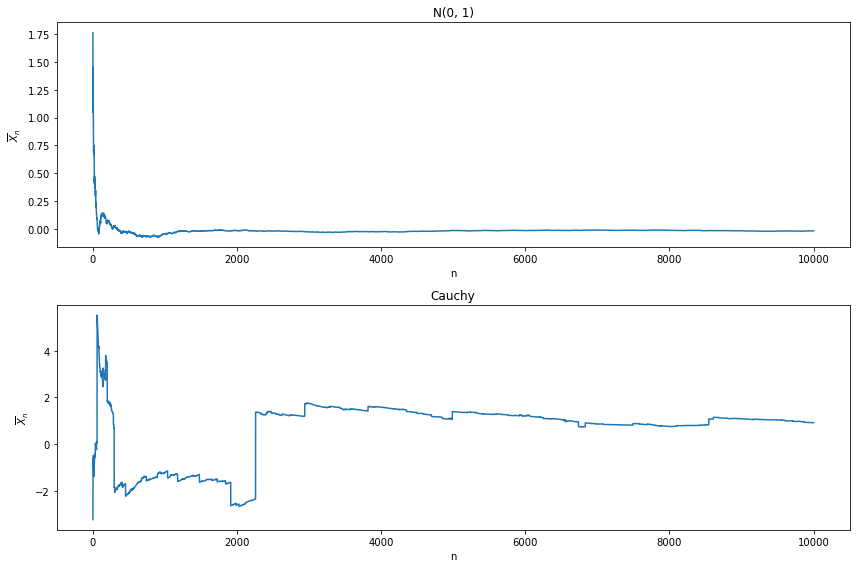
\includegraphics[width=0.9\linewidth,height=0.2\textheight,keepaspectratio]{Figure-04-01}
\end{figure}

The mean on the Cauchy distribution is famously undefined:
\(\overline{X}_ n\) is not going to converge.

\textbf{Exercise 4.7.10}. Let \(X \sim N(0, 1)\) and let \(Y = e^X\).
Find \(\mathbb{E}(Y)\) and \(\mathbb{V}(Y)\).

\textbf{Solution}.

The CDF of \(Y\) is, for \(y > 0\):

\[ F_Y(y) = \mathbb{P}(Y \leq y) = \mathbb{P}(X \leq \log y) = \Phi(\log y) \]

and so the PDF is

\[ f_Y(y) = F'_Y(y) = \frac{d}{dy} \Phi(\log y) = \frac{d \Phi(\log y)}{d \log y} \frac{d \log y}{dy} = \frac{\phi(\log y)}{y}\]

The expected value is

\[ \mathbb{E}(Y) = \int y f_Y(y) dy = \int_0^\infty y \frac{\phi(\log y)}{y} dy = \int_0^\infty \phi(\log y)\; dy = \sqrt{e}\]

The expected value of \(Y^2\) is

\[ \mathbb{E}(Y^2) = \int y^2 f_Y(y) dy = \int_0^\infty y^2 \frac{\phi(\log y)}{y} dy = \int_0^\infty y \phi(\log y)\; dy = e^2\]

and so the variance is

\[ \mathbb{V}(Y) = \mathbb{E}(Y^2) - \mathbb{E}(Y)^2 = e(e - 1) \]

\textbf{Exercise 4.7.11 (Computer Experiment: Simulating the Stock
Market)}. Let \(Y_1, Y_2, \dots\) be independent random variables such
that \(\mathbb{P}(Y_i = 1) = \mathbb{P}(Y_i = -1) = 1/2\). Let
\(X_n = \sum_{i=1}^n Y_i\). Think of \(Y_i = 1\) as ``the stock price
increased by one dollar'' \(Y_i = -1\) as ``the stock price decreased by
one dollar'' and \(X_n\) as the value of the stock on day \(n\).

\textbf{(a)} Find \(\mathbb{E}(X_n)\) and \(\mathbb{V}(X_n)\).

\textbf{(b)} Simulate \(X_n\) and plot \(X_n\) versus \(n\) for
\(n = 1, 2, \dots, 10,000\). Repeat the whole simulation several times.
Notice two things. First, it's easy to ``see'' patterns in the sequence
even though it is random. Second, you will find that the runs look very
different even though they were generated the same way. How do the
calculations in (a) explain the second observation?

\textbf{Solution}.

\textbf{(a)} We have:

\[ \mathbb{E}(X_n) = \mathbb{E}\left( \sum_{i=1}^n Y_i \right) = \sum_{i=1}^n \mathbb{E}(Y_i) = 0 \]

and

\begin{align}
\mathbb{E}(X_n^2) &= \mathbb{E}\left( \left( \sum_{i=1}^n Y_i \right)^2 \right) \\
&= \mathbb{E}\left( \sum_{i=1}^n Y_i^2 + \sum_{i=1}^n \sum_{j = 1, j \neq i}^n Y_i Y_j \right) \\
&= \sum_{i=1}^n \mathbb{E}(Y_i^2) + \sum_{i=1}^n \sum_{j = 1, j \neq i}^n \mathbb{E}(Y_i Y_j) \\
&= \sum_{i=1}^n 1 + \sum_{i=1}^n \sum_{j = 1, j \neq i}^n 0 \\
&= n
\end{align}

so

\[\mathbb{V}(X_n) = \mathbb{E}(X_n^2) - \mathbb{E}(X_n)^2 = n\]

\textbf{(b)}

\begin{python}
import numpy as np
from scipy.stats import norm, bernoulli

N = 10000
B = 20

Y = 2 * bernoulli.rvs(p=1/2, loc=0, size=(B, N), random_state=0) - 1
X = np.cumsum(Y, axis=1)
\end{python}

\begin{python}
import matplotlib.pyplot as plt

plt.figure(figsize=(12, 8))

nn = np.arange(1, N + 1)

z = norm.ppf(0.975)
plt.plot(nn, z * np.sqrt(nn), color='red')
plt.plot(nn, -z * np.sqrt(nn), color='red')
plt.fill_between(nn, z * np.sqrt(nn), -z * np.sqrt(nn), color='red', alpha=0.05)

for b in range(B):
    plt.plot(nn, X[b])
    
plt.show()
\end{python}

\begin{figure}[H]
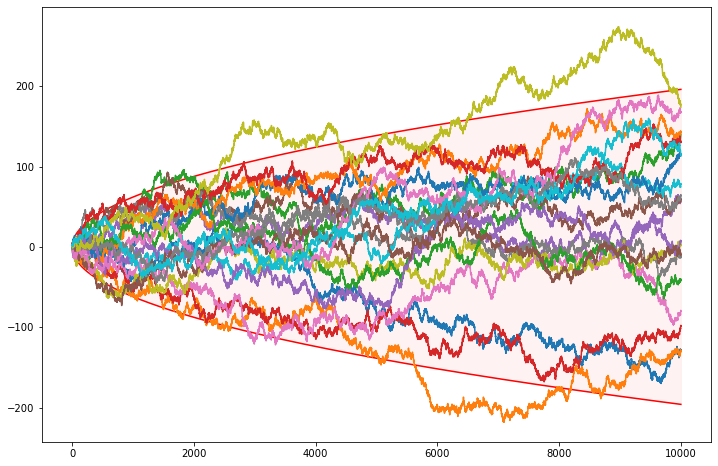
\includegraphics[width=0.9\linewidth,height=0.2\textheight,keepaspectratio]{Figure-04-02}
\end{figure}

The standard deviation is \(\sqrt{n}\) -- it scales up with the square
root of the ``time''. The plot above draws \(z_{\alpha / 2} \sqrt{n}\)
curves -- confidence bands for \(1 - \alpha = 95\%\) -- that contain
most of the randomly generated path.

\textbf{Exercise 4.7.12}. Prove the formulas given in the table at the
beginning of Section 4.4 for the Bernoulli, Poisson, Uniform,
Exponential, Gamma, and Beta. Here are some hints. For the mean of the
Poisson, use the fact that \(e^a = \sum_{x=0}^a a^x / x!\). To compute
the variance, first compute \(\mathbb{E}(X(X - 1))\). For the mean of
the Gamma, it will help to multiply and divide by
\(\Gamma(\alpha + 1) / \beta^{\alpha + 1}\) and use the fact that a
Gamma density integrates to 1. For the Beta, multiply and divide by
\(\Gamma(\alpha + 1) \Gamma(\beta) / \Gamma(\alpha + \beta + 1)\).

\textbf{Solution}.

We will do all expressions in the table instead (other than multinomial
and multivariate normal, where proofs are already provided in the book).

\textbf{Point mass at \(p\)}. Let \(X\) have a point mass at \(p\).
Then:

\begin{itemize}[tightlist]
\item
  \(\mathbb{E}(X) = p \cdot 1 = p\)
\item
  \(\mathbb{E}(X^2) = p^2 \cdot 1 = p^2\)
\item
  \(\mathbb{V}(X) = \mathbb{E}(X^2) - \mathbb{E}(X)^2 = p^2 - p^2 = 0\)
\end{itemize}

\textbf{Bernoulli}. Let \(X \sim \text{Bernoulli}(p)\). Then:

\begin{itemize}[tightlist]
\item
  \$\mathbb{E}(X) = 1 \cdot p + 0 \cdot (1 - p) = p \$
\item
  \(\mathbb{E}(X^2) = 1 \cdot p + 0 \cdot (1 - p) = p\)
\item
  \(\mathbb{V}(X^2) = \mathbb{E}(X^2) - \mathbb{E}(X)^2 = p(1 - p)\)
\end{itemize}

\textbf{Binomial}. Let \(X \sim \text{Binomial}(n, p)\). Then
\(X = \sum_{i=1}^n Y_i\), where \(Y_i \sim \text{Bernoulli}(p)\) are IID
random variables.

\begin{itemize}[tightlist]
\item
  \$\mathbb{E}(X) = \mathbb{E}\left( \sum\emph{\{i=1\}\^{}n Y\_i \right)
  = \sum}\{i=1\}\^{}n \mathbb{E}(Y\_i) = np \$
\item
  \$\mathbb{V}(X) = \mathbb{V}\left(\sum\emph{\{i=1\}\^{}n Y\_i \right)
  = \sum}\{i=1\}\^{}n \mathbb{V}(Y\_i) = np(1-p) \$
\end{itemize}

\textbf{Geometric}. Let \(X \sim \text{Geometric}(p)\). Then:

\begin{align}
\mathbb{E}(X) &= \sum_{k=1}^\infty k p (1 - p)^{k - 1}  \\
&= \sum_{k=1}^\infty p(1-p)^{k-1} + \sum_{k=2}^\infty (k - 1) p(1-p)^{k - 1} \\
&= p \left( 1 + (1 - p) + (1 - p)^2 + \dots \right) + \sum_{k=1}^\infty k p(1-p)^k \\
&= p \left(\frac{1}{1 - (1 - p)}\right) + (1 - p) \sum_{k=1}^\infty k p(1-p)^{k - 1} \\
&= 1 + (1 - p) \mathbb{E}(X)
\end{align}

Solving for the expectation, we get \(\mathbb{E}(X) = 1/p\).

We also have:

\begin{align}
\mathbb{E}(X^2) &= \sum_{k=1}^\infty k^2 p (1 - p)^{k - 1}  \\
&= \sum_{k=1}^\infty k p(1-p)^{k-1} + \sum_{k=2}^\infty (k^2 - k) p(1-p)^{k - 1} \\
&= \mathbb{E}(X) + (1 - p) \sum_{k=1}^\infty (k^2 + k) p(1-p)^{k - 1} \\
&= \mathbb{E}(X) + (1 - p) \mathbb{E}(X) + (1 - p) \sum_{k=1}^\infty k^2 p(1-p)^{k-1} \\
&= \frac{2 - p}{p} + (1 - p) \mathbb{E}(X^2)
\end{align}

Solving for the expectation, we get \(\mathbb{E}(X^2) = (2 - p) / p^2\).

Finally,

\[ \mathbb{V}(X) = \mathbb{E}(X^2) - \mathbb{E}(X)^2 = \frac{2 - p}{p^2} - \frac{1}{p^2} = \frac{1 - p}{p^2} \]

\textbf{Poisson}. Let \(X \sim \text{Poisson}(\lambda)\). Then:

\begin{itemize}
\item
  \$ \mathbb{E}(X) = \sum\emph{\{k=0\}\^{}\infty k
  \frac{\lambda^k e^{-\lambda}}{k!} = \lambda e\^{}\{-\lambda\}
  \sum}\{k=1\}\^{}\infty \frac{\lambda^{k - 1} }{(k - 1)!} =
  \lambda e\^{}\{-\lambda\} \sum\_\{k=0\}\^{}\infty \frac{\lambda^k}{k!}
  = \lambda e\^{}\{-\lambda\} e\^{}\{\lambda\} = \lambda \$
\item
  \$ \mathbb{E}(X\^{}2) = \sum\emph{\{k=0\}\textsuperscript{\infty k}2
  \frac{\lambda^k e^{-\lambda}}{k!} = \lambda \sum}\{k=1\}\^{}\infty k
  \frac{\lambda^{k-1} e^{-\lambda} }{(k-1)!} =
  \lambda \sum\_\{k=0\}\^{}\infty (k + 1)
  \frac{\lambda^{k} e^{-\lambda} }{k!} = \lambda \mathbb{E}(X + 1) =
  \lambda(\lambda + 1) \$
\item
  \$ \mathbb{V}(X) = \mathbb{E}(X\^{}2) - \mathbb{E}(X)\^{}2 =
  \lambda\^{}2 + \lambda - \lambda\^{}2 = \lambda \$
\end{itemize}

\textbf{Uniform}. Let \(X \sim \text{Uniform}(a, b)\). Then:

\begin{itemize}[tightlist]
\item
  \(\mathbb{E}(X) = \int_a^b x \frac{1}{b - a} dx = \frac{a + b}{2}\)
\item
  \(\mathbb{E}(X^2) = \int_a^b x^2 \frac{1}{b - a} dx = \frac{a^2 + ab + b}{3}\)
\item
  \(\mathbb{V}(X) = \mathbb{E}(X^2) - \mathbb{E}(X)^2 = \frac{a^2 + ab + b}{3} - \frac{a^2 + 2ab + b^2}{4} = \frac{(b - a)^2}{12}\)
\end{itemize}

\textbf{Normal}. Let \(X \sim N(\mu, \sigma^2)\). Converting into a
standard normal, we get \(Z = (X - \mu) / \sigma \sim N(0, 1)\). Then:

\begin{itemize}[tightlist]
\item
  \$ \mathbb{E}(X) = \mathbb{E}(\sigma Z + \mu) = \sigma \mathbb{E}(Z) +
  \mu = \mu\$
\item
  \$ \mathbb{V}(X) = \mathbb{V}(\sigma Z + \mu) = \sigma\^{}2
  \mathbb{V}(Z) = \sigma\^{}2\$
\end{itemize}

To prove that the expected value \(Z\) is 0, note that the PDF of \(Z\)
is even, \(\phi(z) = \phi(-z)\), so

\[ \mathbb{E}(Z) = \int_{-\infty}^\infty z \phi(z) dz = \int_{-\infty}^0 z \phi(z) dz + \int_0^\infty z \phi(z) dz = 
\int_0^\infty -z \phi(-z) dz + \int_0^\infty z \phi(z) dz = \int_0^\infty (-z + z)\phi(z) = 0 \]

To prove that the variance of \(Z\) is 0, write out the integral
explicitly for the expectation of \(Z^2\),

\[ \mathbb{E}(Z^2) = \int_{-\infty}^\infty z^2 \phi(z) dz = \frac{1}{\sqrt{2 \pi}} \int_{-\infty}^\infty z^2 e^{-z^2/2} dz
= \left[ \Phi(z) - \frac{1}{\sqrt{2 \pi}}  z e^{-z^2/2} \right]_{-\infty}^\infty = \lim_{x \rightarrow +\infty} \Phi(x) - \lim_{x \rightarrow -\infty} \Phi(x) = 1 - 0 = 1
\]

and so

\[\mathbb{V}(Z) = \mathbb{E}(Z^2) - \mathbb{E}(Z)^2 = 1 - 0 = 1\]

\textbf{Exponential}. Let \(X \sim \text{Exponential}(\beta)\). Then:

\begin{itemize}[tightlist]
\item
  \$ \mathbb{E}(X) = \int\_0\^{}\infty x \frac{1}{\beta} e\^{}\{-x /
  \beta\} dx = \frac{1}{\beta} \int\_0\^{}\infty x e\^{}\{-x / \beta\}
  dx = \frac{1}{\beta} \beta\^{}2 = \beta\$
\item
  \$\mathbb{E}(X\^{}2) = \int\_0\textsuperscript{\infty x}2
  \frac{1}{\beta} e\^{}\{-x / \beta\} dx = \frac{1}{\beta}
  \int\_0\textsuperscript{\infty x}2 e\^{}\{-x / \beta\} dx =
  \frac{1}{\beta} 2\beta\^{}3 = 2 \beta\^{}2 \$
\item
  \$ \mathbb{V}(X) = \mathbb{E}(X\^{}2) - \mathbb{E}(X)\^{}2 =
  2\beta\^{}2 - \beta\^{}2 = \beta\^{}2\$
\end{itemize}

\textbf{Gamma}. Let \(X \sim \text{Gamma}(\alpha, \beta)\). The PDF is

\[ f_X(x) = \frac{\beta^\alpha}{\Gamma(\alpha)} x^{\alpha - 1} e^{-\beta x} \quad \text{for } x > 0 \]

We have:

\begin{align}
\mathbb{E}(X) 
&= \int x f_X(x) dx \\
&= \int_0^\infty x \frac{\beta^\alpha}{\Gamma(\alpha)} x^{\alpha - 1} e^{-\beta x} dx \\
&= \frac{\alpha}{\beta} \int_0^\infty\frac{\beta^{\alpha + 1}}{\Gamma(\alpha + 1)} x^\alpha e^{-\beta x} dx \\
&= \frac{\alpha}{\beta}
\end{align}

where we used that

\begin{itemize}[tightlist]
\item
  \(\alpha \Gamma(\alpha) = \Gamma(\alpha + 1)\),
\item
  and last integral is the PDF of \(\text{Gamma}(\alpha + 1, \beta)\),
  integrated over its entire domain.
\end{itemize}

We also have:

\begin{align}
\mathbb{E}(X^2) 
&= \int x^2 f_X(x) dx \\
&= \int_0^\infty x^2 \frac{\beta^\alpha}{\Gamma(\alpha)} x^{\alpha - 1} e^{-\beta x} dx \\
&= \frac{\alpha (\alpha + 1)}{\beta^2} \int_0^\infty\frac{\beta^{\alpha + 2}}{\Gamma(\alpha + 2)} x^{\alpha + 1} e^{-\beta x} dx \\
&= \frac{\alpha (\alpha + 1)}{\beta^2}
\end{align}

\begin{itemize}[tightlist]
\item
  \(\alpha (\alpha + 1) \Gamma(\alpha + 1) = \Gamma(\alpha + 2)\),
\item
  and last integral is the PDF of \(\text{Gamma}(\alpha + 2, \beta)\),
  integrated over its entire domain.
\end{itemize}

Therefore,

\[ \mathbb{V}(X) = \mathbb{E}(X^2) - \mathbb{E}(X)^2 = \frac{\alpha (\alpha + 1)}{\beta^2} - \frac{\alpha^2}{\beta^2} = \frac{\alpha}{\beta^2} \]

\textbf{Beta}. Let \(X \sim \text{Beta}(\alpha, \beta)\). The PDF is

\[f_X(x) = \frac{\Gamma(\alpha + \beta)}{\Gamma(\alpha) \Gamma(\beta)} x^{\alpha - 1}(1 - x)^{\beta - 1} \quad \text{for } x > 0\]

We have:

\begin{align}
\mathbb{E}(X) 
&= \int x f_X(x) dx \\
&= \int_0^\infty x \frac{\Gamma(\alpha + \beta)}{\Gamma(\alpha) \Gamma(\beta)} x^{\alpha - 1}(1 - x)^{\beta - 1} dx \\
&= \frac{\alpha}{\alpha + \beta} \int_0^\infty \frac{\Gamma(\alpha + \beta + 1)}{\Gamma(\alpha + 1) \Gamma(\beta)} x^{\alpha}(1 - x)^{\beta - 1} dx \\
&= \frac{\alpha}{\alpha + \beta}
\end{align}

where we used that

\begin{itemize}[tightlist]
\item
  \(\alpha \Gamma(\alpha) = \Gamma(\alpha + 1)\),
\item
  \((\alpha + \beta) \Gamma(\alpha + \beta) = \Gamma(\alpha + \beta + 1)\),
\item
  and the last integral is the PDF of
  \(\text{Beta}(\alpha + 1, \beta)\), integrated over its entire domain.
\end{itemize}

We also have:

\begin{align}
\mathbb{E}(X^2) 
&= \int x^2 f_X(x) dx \\
&= \int_0^\infty x^2 \frac{\Gamma(\alpha + \beta)}{\Gamma(\alpha) \Gamma(\beta)} x^{\alpha - 1}(1 - x)^{\beta - 1} dx \\
&= \frac{\alpha (\alpha + 1)}{(\alpha + \beta)(\alpha + \beta + 1)} \int_0^\infty \frac{\Gamma(\alpha + \beta + 2)}{\Gamma(\alpha + 2) \Gamma(\beta)} x^{\alpha + 1}(1 - x)^{\beta - 1} dx \\
&= \frac{\alpha (\alpha + 1)}{(\alpha + \beta)(\alpha + \beta + 1)}
\end{align}

where we used that

\begin{itemize}[tightlist]
\item
  \(\alpha (\alpha + 1) \Gamma(\alpha + 1) = \Gamma(\alpha + 2)\),
\item
  \((\alpha + \beta) (\alpha + \beta + 1) \Gamma(\alpha + \beta + 1) = \Gamma(\alpha + \beta + 2)\),
\item
  and the last integral is the PDF of
  \(\text{Beta}(\alpha + 2, \beta)\), integrated over its entire domain.
\end{itemize}

Therefore,

\[ \mathbb{V}(X) = \mathbb{E}(X^2) - \mathbb{E}(X)^2 = \frac{\alpha (\alpha + 1)}{(\alpha + \beta)(\alpha + \beta + 1)} - \frac{\alpha^2}{(\alpha + \beta)^2} = \frac{\alpha \beta}{(\alpha + \beta)^2 (\alpha + \beta + 1)} \]

\textbf{t-student}. Let \(X \sim t_\nu\). The PDF for the t-student
distribution is

\[ f_X(x) = \frac{1}{\sqrt{v \pi}} \frac{\Gamma\left(\frac{\nu + 1}{2}\right)}{\Gamma\left(\frac{\nu}{2}\right)} \frac{1}{\left(1 + \frac{x^2}{\nu} \right)^{(\nu + 1)/2}} \]

Since the PDF is even, \(f_X(x) = f_X(-x)\), the expectation will be 0
when it is defined:

\[ \mathbb{E}(X) = \int_{-\infty}^\infty x f_X(x) dx = \int_{-\infty}^0 x f_X(x) dx + \int_0^\infty x f_X(x) dx = 
\int_0^\infty -x f_X(-x) dx + \int_0^\infty x f_X(x) dx = \int_0^\infty (-x + x)f_X(x) dx = 0 \]

But

\[ \mathbb{E}(X) = \int_{-\infty}^\infty x f_X(x) dx = \frac{1}{\sqrt{v \pi}} \frac{\Gamma\left(\frac{\nu + 1}{2}\right)}{\Gamma\left(\frac{\nu}{2}\right)} \int_{-\infty}^\infty x  \left(1 + \frac{x^2}{\nu} \right)^{-(\nu + 1)/2} dx \]

For the expectation of \(X^2\), assuming it is defined, we have:

\begin{align}
\mathbb{E}(X^2) &= \int_{-\infty}^\infty x^2 f_X(x) dx \\
&= \frac{1}{\sqrt{v \pi}} \frac{\Gamma\left(\frac{\nu + 1}{2}\right)}{\Gamma\left(\frac{\nu}{2}\right)} \int_{-\infty}^\infty x^2 \left( 1 + \frac{x^2}{\nu}\right)^{-(\nu + 1) / 2} dx \\
&= \frac{\nu}{\sqrt{\pi}} \frac{\Gamma\left(\frac{\nu + 1}{2}\right)}{\Gamma\left(\frac{\nu}{2}\right)} \int_0^1 y^{\nu /2 - 2} \left( 1 - y \right)^{1 / 2} dy \\
&= \frac{\nu}{\sqrt{\pi}} \frac{\Gamma\left(\frac{\nu + 1}{2}\right)}{\Gamma\left(\frac{\nu}{2}\right)} \frac{\Gamma\left(\frac{\nu}{2} - 1\right) \Gamma\left(\frac{3}{2}\right)}{\Gamma\left(\frac{\nu + 1}{2}\right)} \\
&= \frac{\nu}{\nu - 2}
\end{align}

where we used:

\begin{itemize}[tightlist]
\item
  A variable replacement \(y = \left( 1 + \frac{x^2}{\nu} \right)^{-1}\)
\item
  The property that
  \(\int_0^1 y^{p - 1} (1 - y)^{q - 1} dy = \frac{\Gamma(p) \Gamma(q)}{\Gamma(p + q)}\),
  since this is the integral of the PDF of \(\Gamma(p, q)\) scaled by a
  factor of \(\frac{\Gamma(p) \Gamma(q)}{\Gamma(p + q)}\), with
  \(p = \nu / 2 - 1\), \(q = 3/2\)
\item
  \(\Gamma(3 / 2) = \sqrt{\pi}\)
\end{itemize}

Finally,

\[ \mathbb{V}(X) = \mathbb{E}(X^2) - \mathbb{E}(X)^2 = \frac{\nu}{\nu - 2} \]

\emph{Reference: https://math.stackexchange.com/a/1502519}

\textbf{\(\chi^2\) distribution}. Let \(X \sim \chi^2_k\). Then \(X\)
has the same distributions as the sum of squares of \(k\) IID standard
Normal random variables, \(X = \sum_{i=1}^k Z_i^2\),
\(Z_i \sim N(0, 1)\).

The expectation of \(X\) can then be computed:

\[ \mathbb{E}(X) = \mathbb{E}\left( \sum_{i=1}^k Z_i^2 \right) = \sum_{i=1}^k \mathbb{E}(Z_i^2) = \sum_{i=1}^k (\mathbb{V}(Z_i) + \mathbb{E}(Z_i)^2) = \sum_{i=1}^k (1 + 0) = k \]

The expectation of \(X^2\) is:

\begin{align}
\mathbb{E}(X^2) &= \mathbb{E}\left( \left( \sum_{i=1}^k Z_i^2 \right)^2 \right) \\
&= \mathbb{E}\left( \sum_{i=1}^k Z_i^4 + \sum_{i=1}^k \sum_{j=1; j \neq i}^k Z_i^2 Z_j^2 \right) \\
&= \sum_{i=1}^k \mathbb{E}(Z_i^4) + \sum_{i=1}^k \sum_{j=1; j \neq i}^k \mathbb{E}(Z_i^2) \mathbb{E}(Z_j^2)
\end{align}

But we have:

\[ \mathbb{E}(Z_i^2) = \mathbb{V}(Z_i) + \mathbb{E}(Z_i)^2 = 1 + 0 = 1 \]

and, using moment generating functions,

\[M_Z(t) = e^{t^2 / 2}\]

and taking the fourth derivative,

\[ M_Z^{(4)}(t) = 3 M_Z^{(2)}(t) + t M_Z^{(3)}(t)\]

Setting \(t = 0\) gives us \(\mathbb{E}(Z_i^4) = 3\).

Replacing it back on the expectation expression for \(X^2\),

\[
\mathbb{E}(X^2) = \sum_{i=1}^k 3 + \sum_{i=1}^k \sum_{j=1; j \neq i}^k 1 \cdot 1 = 3k + k(k-1) = k^2 + 2k
\]

Therefore,

\[ \mathbb{V}(X) = \mathbb{E}(X^2) - \mathbb{E}(X)^2 = k^2 + 2k - k^2 = 2k \]

\emph{The proofs for the multinomial and mutivariate normal distribution
expressions are provided in the book text (and there are notes above).}

\textbf{Exercise 4.7.13}. Suppose we generate a random variable \(X\) in
the following way. First we flip a fair coin. If the coin is heads, take
\(X\) to have a \(\text{Uniform}(0, 1)\) distribution. If the coin is
tails, take \(X\) to have a \(\text{Uniform}(3, 4)\) distribution.

\textbf{(a)} Find the mean of \(X\).

\textbf{(b)} Find the standard deviation of \(X\).

\textbf{Solution}. We have \(X = C U_1 + (1 - C)U_2\), where
\(C \sim \text{Bernoulli}(1/2)\), \(U_1 \sim \text{Uniform}(0, 1)\) and
\(U_2 \sim \text{Uniform}(3, 4)\) are all independent.

\textbf{(a)}

\[\mathbb{E}(X) = \mathbb{E}(CU_1 + (1 - C)U_2) = \mathbb{E}(C)\mathbb{E}(U_1) + (1 - \mathbb{E}(C))\mathbb{E}(U_2) = \frac{1}{2} \left(\frac{1}{2} + \frac{7}{2}\right) = 2\]

\textbf{(b)}

\[ X^2 = (CU_1 + (1 - C)U_2)^2 = C^2U_1^2 + (1 - C)^2 U_2^2 + 2C(1 - C)U_1U_2 = C^2U_1^2 + (1 - C)^2 U_2^2 \]

so

\begin{align}
\mathbb{E}(X^2) &= \mathbb{E}(C^2)\mathbb{E}(U_1^2) + \mathbb{E}((1 - C)^2) \mathbb{E}(U_2^2) \\
&= \mathbb{E}(C) \mathbb{E}(U_1^2) + \mathbb{E}(1 - C) \mathbb{E}(U_2^2) \\
&= \frac{1}{2} \left( \frac{1}{3} + \frac{37}{3} \right) = \frac{19}{3}
\end{align}

and then

\[ \mathbb{V}(X) = \mathbb{E}(X^2) - \mathbb{E}(X)^2 = \frac{19}{3} - 2^2 = \frac{7}{3} \]

and so the standard deviation is \(\sqrt{\mathbb{V}(X)} = \sqrt{7/3}\).

\textbf{Exercise 4.17.14}. Let \(X_1, \dots, X_m\) and
\(Y_1, \dots, Y_n\) be random variables and let \(a_1, \dots, a_m\) and
\(b_1, \dots, b_n\) be constants. Show that

\[ \text{Cov}\left( \sum_{i=1}^m a_i X_i , \sum_{j=1}^n b_j Y_j \right) = \sum_{i=1}^m \sum_{j=1}^n a_i b_j \text{Cov}(X_i, Y_j) \]

\textbf{Solution}. We have:

\begin{align}
\text{Cov}\left(\sum_{i=1}^m a_i X_i, Y\right) &= \mathbb{E}\left(\left( \sum_{i=1}^m a_i X_i \right) Y\right) - \mathbb{E}\left( \sum_{i=1}^m a_i X_i \right) \mathbb{E}(Y) \\
&= \sum_{i=1}^m \mathbb{E}(a_i X_i Y) - \left( \sum_{i=1}^m a_i \mathbb{E}(X_i) \right) \mathbb{E}(Y) \\
&= \sum_{i=1}^m \mathbb{E}(a_i X_i Y) -  a_i \mathbb{E}(X_i) \mathbb{E}(Y) \\
&= \sum_{i=1}^m a_i \text{Cov}(X_i, Y)
\end{align}

and, since \(\text{Cov}(A, B) = \text{Cov}(B, A)\),

\[ \text{Cov}\left(X, \sum_{j=1}^n b_j Y_j \right) = \sum_{j=1}^n b_i \text{Cov}(X, Y_j) \]

Applying this for each \(X_i\), we get the result.

\textbf{Exercise 4.17.15}. Let

\[ f_{X, Y} = \begin{cases}
\frac{1}{3} (x + y) &\text{if } 0 \leq x \leq 1, 0 \leq y \leq 2 \\
0 &\text{otherwise}
\end{cases}\]

Find \(\mathbb{V}(2X - 3Y + 8)\).

\textbf{Solution}. Let \(r(x, y) = 2x - 3y\). Then:

\[ \mathbb{V}(2X - 3Y + 8) = \mathbb{V}(2X - 3Y) = \mathbb{V}(r(X, Y)) \]

Calculating the expectation of \(r(X, Y)\) and \(r(X, Y)^2\):

\[ \mathbb{E}(r(X, Y)) = \int_0^1 \int_0^2 r(x, y) f(x, y) dy dx = \int_0^1 \int_0^2 \frac{1}{3}(2x - 3y)(x + y) dy dx 
= \int_0^1 \frac{2}{3}(2x^2 - x - 4) dx = -\frac{23}{9} \]

and

\[ \mathbb{E}(r(X, Y)^2) = \int_0^1 \int_0^2 r(x, y)^2 f(x, y) dy dx = \int_0^1 \int_0^2 \frac{1}{3}(2x - 3y)^2(x + y) dy dx 
= \int_0^1 \frac{4}{3}(2x^3 - 4x^2 - 2x + 9) dx = \frac{86}{9} \]

and so

\[ \mathbb{V}(r(X, Y)) = \mathbb{E}(r(X, Y)^2) - \mathbb{E}(r(X, Y))^2 = \frac{86}{9} - \frac{23^2}{9^2} = \frac{245}{81} \]

\textbf{Exercise 4.17.16}. Let \(r(x)\) be a function of \(x\) and let
\(s(y)\) be a function of \(y\). Show that

\[ \mathbb{E}(r(X) s(Y) | X) = r(X) \mathbb{E}(s(Y) | X) \]

Also, show that \(\mathbb{E}(r(X) | X) = r(X)\).

\textbf{Solution}. We have:

\[ \mathbb{E}(r(X) s(Y) | X = x) = \int r(x) s(y) f(x, y) dy = r(x) \int s(y) f(x, y) dy = r(x) \mathbb{E}(s(Y) | X = x) \]

and so the random variable \(\mathbb{E}(r(X) s(Y) | X)\) takes the same
value as the variable \(r(X) \mathbb{E}(s(Y) | X)\) for each \(X = x\)
-- therefore the random variables are equal.

In particular, when \(s(y) = 1\) for all \(y\), we have
\(\mathbb{E}(r(X) | X) = r(X)\).

\textbf{Exercise 4.17.17}. Prove that

\[ \mathbb{V}(Y) = \mathbb{E} \mathbb{V} (Y | X) + \mathbb{V} \mathbb{E} (Y | X) \]

Hint: Let \(m = \mathbb{E}(Y)\) and let
\(b(x) = \mathbb{E}(Y | X = x)\). Note that
\(\mathbb{E}(b(X)) = \mathbb{E} \mathbb{E}(Y | X) = \mathbb{E}(Y) = m\).
Bear in mind that \(b\) is a function of \(x\). Now write

\[\mathbb{V}(Y) = \mathbb{E}((Y - m)^2) = \mathbb{E}(((Y - b(X)) + (b(X) - m))^2)\]

Expand the square and take the expectation. You then have to take the
expectation of three terms. In each case, use the rule of iterated
expectation,
i.e.~\(\mathbb{E}(\text{stuff}) = \mathbb{E}(\mathbb{E}(\text{stuff} | X))\).

\textbf{Solution}. We have:

\begin{align}
\mathbb{V}(Y) &= \mathbb{E}(Y^2) - \mathbb{E}(Y)^2 \\
&= \mathbb{E}(\mathbb{E}(Y^2 | X)) - \mathbb{E}(\mathbb{E}(Y | X))^2 \\
&= \mathbb{E}\left( \mathbb{V}(Y | X) + \mathbb{E}(Y | X)^2 \right) - \mathbb{E}(\mathbb{E}(Y | X))^2 \\
&= \mathbb{E}(\mathbb{V}(Y | X)) + \left( \mathbb{E}(\mathbb{E}(Y | X)^2) - \mathbb{E}(\mathbb{E}(Y | X))^2 \right) \\
&= \mathbb{E} (\mathbb{V}(Y | X) + \mathbb{V}(\mathbb{E}(Y | X))
\end{align}

\textbf{Exercise 4.17.18}. Show that if \$\mathbb{E}(X \textbar{} Y = y)
= c \$ for some constant \(c\) then \(X\) and \(Y\) are uncorrelated.

\textbf{Solution}. We have:

\[ \mathbb{E}(XY) = \int \mathbb{E}(XY | Y = y) dF_Y(y) = \int y \mathbb{E}(X | Y = y) dF_Y(y) = \int cy \mathbb{E}(X | Y = y) dF_Y(y) = c \; \mathbb{E}(Y)\]

and

\[ \mathbb{E}(X) = \mathbb{E}(\mathbb{E}(X | Y)) = \mathbb{E}(c) = c \]

so \(\mathbb{E}(XY) = \mathbb{E}(X) \mathbb{E}(Y)\), and so
\(\text{Cov}(X, Y) = 0\), and so \(X\) and \(Y\) are uncorrelated.

\textbf{Exercise 4.17.19}. This question is to help you understand the
idea of \textbf{sampling distribution}. Let \(X_1, \dots, X_n\) be IID
with mean \(\mu\) and variance \(\sigma^2\). Let
\(\overline{X}_n  = n^{-1}\sum_{i=1}^n X_i\). Then \(\overline{X}_n\) is
a \textbf{statistic}, that is, a function of the data. Since
\(\overline{X}_n\) is a random variable, it has a distribution. This
distribution is called the \emph{sampling distribution of the
statistic}. Recall from Theorem 4.16 that
\(\mathbb{E}(\overline{X}_n) = \mu\) and
\(\mathbb{V}(\overline{X}_n) = \sigma^2 / n\). Don't confuse the
distribution of the data \(f_X\) and the distribution of the statistic
\(f_{\overline{X}_n}\). To make this clear, let
\(X_1, \dots, X_n \sim \text{Uniform}(0, 1)\). Let \(f_X\) be the
density of the \(\text{Uniform}(0, 1)\). Plot \(f_X\). Now let
\(\overline{X}_n = n^{-1} \sum_{i=1}^n X_i\). Find
\(\mathbb{E}(\overline{X}_n)\) and \(\mathbb{V}(\overline{X}_n)\). Plot
them as a function of \(n\). Comment. Now simulate the distribution of
\(\overline{X}_n\) for \(n = 1, 5, 25, 100\). Check the simulated values
of \(\mathbb{E}(\overline{X}_n)\) and \(\mathbb{V}(\overline{X}_n)\)
agree with your theoretical calculations. What do you notice about the
sampling distribution of \(\overline{X}_n\) as it increases?

\textbf{Solution}.

\[ \mathbb{E}\left(\overline{X}_n\right) = \mathbb{E}\left(n^{-1} \sum_{i=1}^n X_i \right) = n^{-1} \sum_{i=1}^n \mathbb{E}(X_i) = \frac{1}{2} \]

and

\[ \mathbb{V}\left(\overline{X}_n\right) = \mathbb{V}\left(n^{-1} \sum_{i=1}^n X_i \right) = n^{-2} \sum_{i=1}^n \mathbb{V}(X_i) = \frac{1}{12 n} \]

\begin{python}
import numpy as np

np.random.seed(0)

B = 1000

E_overline_X = np.empty(100)
V_overline_X = np.empty(100)

for n in range(1, 101):
    X_n = np.random.uniform(low=0, high=1, size=(B, n)).mean(axis=1)
    E_overline_X[n - 1] = X_n.mean()
    V_overline_X[n - 1] = X_n.var()
\end{python}

\begin{python}
import matplotlib.pyplot as plt

plt.figure(figsize=(12, 8))

ax = plt.subplot(212)
ax.hlines(0, xmin=-0.5, xmax=0, color='C0')
ax.hlines(1, xmin=0, xmax=1, color='C0')
ax.hlines(0, xmin=1, xmax=1.5, color='C0')
ax.vlines([0, 1], ymin=0, ymax=1, color='C0', linestyle='dashed')
ax.set_xlabel('x')
ax.set_ylabel(r'$f_X(x)$')
ax.set_title('Density of Uniform(0, 1)')

nn = np.arange(1, 101)

ax = plt.subplot(221)
ax.plot(nn, 1/2 * np.ones(100), label='Calculated')
ax.plot(nn, E_overline_X, label='Measured')
ax.set_xlabel('n')
ax.set_ylabel(r'$\mathbb{E}(\overline{X}_n)$')
ax.set_title('Sampling distribution mean')
ax.legend(loc='lower right')

ax = plt.subplot(222)
ax.plot(nn, 1 / (12 * nn), label='Calculated')
ax.plot(nn, V_overline_X, label='Measured')
ax.set_xlabel('n')
ax.set_yscale('log')
ax.set_ylabel(r'$\mathbb{V}(\overline{X}_n)$')
ax.set_title('Sampling distribution variance')
ax.legend(loc='upper right')

plt.tight_layout()
plt.show()
\end{python}

\begin{figure}[H]
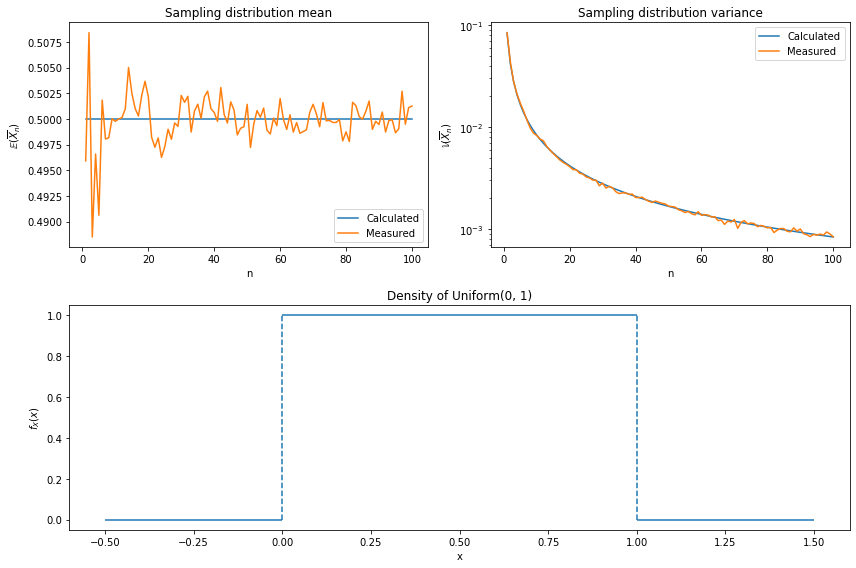
\includegraphics[width=0.9\linewidth,height=0.2\textheight,keepaspectratio]{Figure-04-03}
\end{figure}

Calculated and simulated values agree.

\textbf{Exercise 4.17.20}. Prove Lemma 4.20.

If \(a\) is a vector and \(X\) is a random vector with mean \(\mu\) and
variance \(\Sigma\) then

\[ \mathbb{E}(a^T X) = a^T \mu
\quad \text{and} \quad
\mathbb{V}(a^T X) = a^T \Sigma a \]

If \(A\) is a matrix then

\[ \mathbb{E}(A X) = A \mu
\quad \text{and} \quad
\mathbb{V}(AX) = A \Sigma A^T \]

\textbf{Solution}.

We have:

\[ \mathbb{E}(a^T X) = \begin{pmatrix}
\mathbb{E}(a_1 X_1) \\
\mathbb{E}(a_2 X_2) \\
\cdots \\
\mathbb{E}(a_k X_k)
\end{pmatrix} = \begin{pmatrix}
a_1 \mathbb{E}(X_1) \\
\mathbb{E}(X_2) \\
\cdots \\
\mathbb{E}(X_k)
\end{pmatrix} = a^T \mu \]

and

\[ \mathbb{V}(a^T X) = \mathbb{E}((a^T (X - \mu) (a^T(X - \mu))^T) = \mathbb{E}((a^T (X - \mu) (X - \mu)^T a) = a^T \Sigma a \]

Similarly, for the matrix case,

\[ \mathbb{E}(AX) = \begin{pmatrix}
\mathbb{E}\left( \sum_{j=1}^k a_{1, j} X_j \right) \\
\mathbb{E}\left( \sum_{j=1}^k a_{2, j} X_j \right) \\
\cdots \\
\mathbb{E}\left( \sum_{j=1}^k a_{k, j} X_j \right) \\
\end{pmatrix} = \begin{pmatrix}
\sum_{j=1}^k a_{1, j} \mathbb{E}(X_j) \\
\sum_{j=1}^k a_{2, j} \mathbb{E}(X_j) \\
\cdots \\
\sum_{j=1}^k a_{k, j} \mathbb{E}(X_j) \\
\end{pmatrix} = A \mu \]

and

\[ \mathbb{V}(A X) = \mathbb{E}((A (X - \mu) (A(X - \mu))^T) = \mathbb{E}((A (X - \mu) (X - \mu)^T A^T) = A \Sigma A^T \]

\textbf{Exercise 4.17.21}. Let \(X\) and \(Y\) be random variables.
Suppose that \(\mathbb{E}(Y|X) = X\). Show that
Cov\((Y, X) = \mathbb{V}(X)\).

\textbf{Solution}. We know that \[Cov(X, Y)\]
\[= \mathbb{E}(X \cdot Y) - \mathbb{E}(X) \cdot \mathbb{E}(Y)\]
\[= \mathbb{E}(X \cdot Y) - \mathbb{E}(X) \cdot \mathbb{E}(\mathbb{E}(Y|X))\]
\[= \mathbb{E}(X\cdot Y) - \mathbb{E}(X) \cdot \mathbb{E}(X)\]

Hence we only need to show that
\[\mathbb{E}(X\cdot Y) = \mathbb{E}(X \cdot \mathbb{E}(Y|X))\]

This is true, since \(E(Y) = EE(Y|X)\). Therefore \[Cov(X, Y)\]
\[= \mathbb{E}(X\cdot Y) -  \mathbb{E}(X) \cdot \mathbb{E}(X)\]
\[= \mathbb{E}(X \cdot \mathbb{E}(Y|X)) -  \mathbb{E}(X) \cdot \mathbb{E}(X)\]
\[= \mathbb{E}(X\cdot X) -  \mathbb{E}(X) \cdot \mathbb{E}(X)\]
\[= Cov(X, X)\] \[= V(X)\]



% Chapter 5
\section{5. Inequalities}\label{inequalities}

\subsection{5.1 Markov and Chebyshev
Inequalities}\label{markov-and-chebyshev-inequalities}

\textbf{Theorem 5.1 (Markov's Inequality)}. Let \(X\) be a non-negative
random variable and suppose that \(\mathbb{E}(X)\) exists. For any
\(t > 0\),

\[ \mathbb{P}(X > t) \leq \frac{\mathbb{E}(X)}{t} \]

\textbf{Proof}.

\[ 
\mathbb{E}(X)
=\int_0^\infty xf(x) dx
=\int_0^t xf(x) dx + \int_t^\infty xf(x) dx
\geq \int_t^\infty xf(x) dx
\geq t \int_t^\infty f(x) dx
= t \mathbb{P}(X > t)
\]

\textbf{Theorem 5.2 (Chebyshev's Inequality)}. Let
\(\mu = \mathbb{E}(X)\) and \(\sigma^2 = \mathbb{V}(X)\). Then,

\[ \mathbb{P}(|X - \mu| \geq t) \leq \frac{\sigma^2}{t^2} 
\quad \text{and} \quad
\mathbb{P}(|Z| \geq k) \leq \frac{1}{k^2} \]

where \(Z = (X - \mu) / \sigma\). In particular,
\(\mathbb{P}(|Z| > 2) \leq 1/4\) and \(\mathbb{P}(|Z| > 3) \leq 1/9\).

\textbf{Proof}. We use Markov's inequality to conclude that

\[ \mathbb{P}(|X - \mu| \geq t) = \mathbb{P}(|X - \mu|^2 \geq t^2) \leq \frac{\mathbb{E}(X - \mu)^2}{t^2} = \frac{\sigma^2}{t^2} \]

The second part follows by setting \(t = k \sigma\).

\subsection{5.2 Hoeffding's Inequality}\label{hoeffdings-inequality}

Hoeffding's inequality is similar in spirit to Markov's inequality but
it is a sharper inequality. We present the result here in two parts. The
proofs are in the technical appendix.

\textbf{Theorem 5.4}. Let \(Y_1, \dots, Y_n\) be independent
observations such that \(\mathbb{E}(Y_i) = 0\) and
\(a_i \leq Y_i \leq b_i\). Let \(\epsilon > 0\). Then, for any
\(t > 0\),

\[ \mathbb{P}\left( \sum_{i=1}^n Y_i \geq \epsilon \right) \leq e^{-t\epsilon} \prod_{i=1}^n e^{t^2(b_i - a_i)^2 / 8} \]

\textbf{Theorem 5.5}. Let \(X_1, \dots, X_n \sim \text{Bernoulli}(p)\).
Then, for any \(\epsilon > 0\),

\[ \mathbb{P}(|\overline{X}_n - p| > \epsilon) \leq 2e^{-2n\epsilon^2} \]

Hoeffding's inequality gives us a simple way go create a
\textbf{confidence interval} for a binomial parameter \(p\). We will
discuss confidence intervals later but here is the basic idea. Let
\(\alpha > 0\) and let

\[ \epsilon_n = \left\{ \frac{1}{2n} \log \left( \frac{2}{\alpha} \right) \right\}^{1/2} \]

By Hoeffding's inequality,

\[ \mathbb{P}(|\overline{X}_n - p| > \epsilon_n) \leq 2e^{-2n\epsilon_n^2} = \alpha \]

Let \(C = (\overline{X}_n - \epsilon, \overline{X}_n + \epsilon)\).
Then,
\(\mathbb{P}(\text{not } C \in p) = \mathbb{P}(|\overline{X}_n - p| > \epsilon) \leq \alpha\).
Hence, \(\mathbb{P}(p \in C) \geq 1 - \alpha\), that is, the random
interval \(C\) traps the true parameter \(p\) with probability
\(1 - \alpha\); we call \(C\) a \(1 - \alpha\) confidence interval. More
on this later.

\subsection{5.3 Cauchy-Schwartz and Jensen
Inequalities}\label{cauchy-schwartz-and-jensen-inequalities}

This section contains two inequalities on expected values that are often
useful.

\textbf{Theorem 5.7 (Cauchy-Schwartz Inequalities)}. If \(X\) and \(Y\)
have finite variances then

\[ \mathbb{E}|XY| \leq \sqrt{\mathbb{E}\left(X^2\right) \mathbb{E}\left(Y^2\right)} \]

Recall that a function \(g\) is \textbf{convex} if for each \(x, y\) and
each \(\alpha \in [0, 1]\),

\[ g(\alpha x + (1 - \alpha)y) \leq \alpha g(x) + (1 - \alpha) g(y) \]

If \(g\) is twice differentiable, then the convexity reduces to checking
that \(g''(x) \geq 0\) for all \(x\). It can be shown that if \(g\) is
convex then it lies above any line that touches \(g\) at some point,
called a tangent line. A function \(g\) is \textbf{concave} if \(-g\) is
convex. Examples of convex functions are \(g(x) = -x^2\) and
\(g(x) = \log x\).

\textbf{Theorem 5.8 (Jensen's Inequality)}. If \(g\) is convex then

\[ \mathbb{E}g(X) \geq g(\mathbb{E}X) \]

If \(g\) is concave then

\[ \mathbb{E}g(X) \leq g(\mathbb{E}X) \]

\textbf{Proof}. Let \(L(x) = a + bx\) be a line, tangent to the \(g(x)\)
at the point \(\mathbb{E}(X)\). Since \(g\) is convex, it lies above the
line \(L(x)\). So,

\[ \mathbb{E}g(X) \geq \mathbb{E}L(X) = \mathbb{E}(a + bX) = a + b\mathbb{E}(X) = L(\mathbb{E}(X)) = g(\mathbb{E}(X))\]

From Jensen's inequality we see that
\(\mathbb{E}X^2 \geq (\mathbb{E}X)^2\) and
\(\mathbb{E}(1/X) \geq 1 / \mathbb{E}(X)\). Since log is concave,
\(\mathbb{E}(\log X) \leq \log \mathbb{E}(X)\). For example, suppose
that \(X \sim N(3, 1)\). Then \(\mathbb{E}(1 / X) \geq 1/3\).

\subsection{5.4 Technical Appendix: Proof of Hoeffding's
Inequality}\label{technical-appendix-proof-of-hoeffdings-inequality}

We will make use of the exact form of Taylor's theorem: if \(g\) is a
smooth function, then there is a number \(\xi \in (0, u)\) such that
\(g(u) = g(0) + u g'(0) + \frac{u^2}{2}g''(\xi)\).

\textbf{Proof of Theorem 5.4}. For any \(t > 0\), we have, from Markov's
inequality, that

\[ \mathbb{P}\left( \sum_{i=1}^n Y_i \geq \epsilon \right) = \mathbb{P}\left( t \sum_{i=1}^n Y_i \geq t \epsilon \right)
= \mathbb{P}\left( e^{t \sum_{i=1}^n Y_i} \geq e^{t \epsilon} \right) \leq e^{-t\epsilon} \mathbb{E}\left( e^{t \sum_{i=1}^n Y_i}\right) = e^{-t\epsilon} \prod_i \mathbb{E}\left(e^{tY_i}\right) \]

Since \(a_i \leq Y_i \leq b_i\), we can write \(Y_i\) as a convex
combination of \(a_i\) and \(b_i\), namely,
\(Y_i = \alpha b_i + (1 - \alpha) a_i\) where
\(\alpha = (Y_i - a_i) / (b_i - a_i)\). So, by the convexity of
\(e^{ty}\) we have

\[ e^{tY_i} \leq \frac{Y_i - a_i}{b_i - a_i} e^{tb_i} + \frac{b_i - Y_i}{b_i - a_i} e^{ta_i} \]

Take expectations of both sides and use the fact that
\(\mathbb{E}(Y_i) = 0\) to get

\[ \mathbb{E}e^{tY_i} \leq - \frac{a_i}{b_i - a_i} e^{tb_i} + \frac{b_i}{b_i - a_i} e^{ta_i} = e^{g(u)} \]

where \(u = t(b_i - a_i)\),
\(g(u) = -\gamma u + \log (1 - \gamma + \gamma e^u)\) and
\(\gamma = -a_i / (b_i - a_i)\).

Note that \(g(0) = g'(0) = 0\). Also, \(g''(u) \leq 1/4\) for all
\(u > 0\). By Taylor's theorem, there is a \(\xi \in (0, u)\) such that

\[ g(u) = g(0) + u g'(0) + \frac{u^2}{2} g(\xi) = \frac{u^2}{2} g(\xi) \leq \frac{u^2}{8} = \frac{t^2(b_i - a_i)^2}{8} \]

Hence,

\[ \mathbb{E}e^{tY_i} \leq e^{g(u)} \leq e^{t^2(b_i - a_i)^2/8} \]

and the result follows.

\textbf{Proof of Theorem 5.5}. Let \(Y_i = (1 / n)(X_i - p)\). Then
\(\mathbb{E}(Y_i) = 0\) and \(a \leq Y_i \leq b\) where \(a = -p/n\) and
\(b = (1 - p) / n\). Also, \((b - a)^2 = 1/n^2\). Applying Theorem 5.4
we get

\[ \mathbb{P}\left(\overline{X}_n - p > \epsilon\right) = \mathbb{P}\left( \sum_i Y_i > \epsilon \right) \leq e^{-t\epsilon} e^{t^2/(8n)}\]

The above holds for any \(t > 0\). In particular, take
\(t = 4n\epsilon\) and we get
\(\mathbb{P}\left(\overline{X}_n - p > \epsilon\right)  \leq e^{-2n\epsilon^2}\).
By a similar argument we can show that
\(\mathbb{P}\left(\overline{X}_n - p < \epsilon\right)  \leq e^{-2n\epsilon^2}\).
Putting those together we get
\(\mathbb{P}\left(|\overline{X}_n - p| >  \epsilon\right)  \leq 2e^{-2n\epsilon^2}\).

\subsection{5.6 Exercises}\label{exercises}

\textbf{Exercise 5.6.1}. Let \(X \sim \text{Exponential}(\beta)\). Find
\(\mathbb{P}(|X - \mu_X| > k \sigma_X)\) for \(k > 1\). Compare this to
the bound you get from Chebyshev's inequality.

\textbf{Solution}.

Let \(F\) be the CDF of \(X\). We have:

\begin{align}
\mathbb{P}(|X - \mu_X| > k \sigma_X) &= 1 - \mathbb{P}(-k \sigma_X < X - \mu_X < k \sigma_X) \\
&= 1 - \mathbb{P}(\mu_X - k \sigma_X < X < \mu_X + k \sigma_X) \\
&= 1 - F(\mu_X + k \sigma_X) + F(\mu_X - k \sigma_X) \\
&= 1 - 1 + \exp\left\{ -\frac{\left(\beta + k \beta\right)^+}{\beta} \right\} + 1 - \exp\left\{-\frac{\left(\beta - k \beta\right)^+}{\beta} \right\} \\
&= 1 + e^{-(1+k)^+ } - e^{-(1-k)^+} 
\end{align}

where \((a)^+ = \max \{ a, 0 \}\).

On the other hand, Chebyshev's bound provides, for \(t = k\sigma_X\),

\[ \mathbb{P}(|X - \mu_X| \geq k \sigma_X) \leq \frac{\sigma_X^2}{k^2 \sigma_X^2}  = \frac{1}{k^2} \]

which is a weaker bound.

\begin{python}
import numpy as np
import matplotlib.pyplot as plt

def f(k):
    return 1 + np.exp(-np.maximum(1+k, 0)) - np.exp(-np.maximum(1 - k, 0))

def chebyshev(k):
    # Limit upper bound to 1, since probability is always under 1
    return np.minimum(1 / (k**2), 1)

kk = np.arange(0.01, 10, step = 0.01)

plt.figure(figsize=(12, 8))

plt.plot(kk, f(kk), label='Calculated probability')
plt.plot(kk, chebyshev(kk), label='min(Chebyshev bound, 1)')
plt.yscale('log')
plt.xlabel('k')
plt.ylabel('Probability bound')
plt.legend(loc='lower left')
plt.show()
\end{python}

\begin{figure}[H]
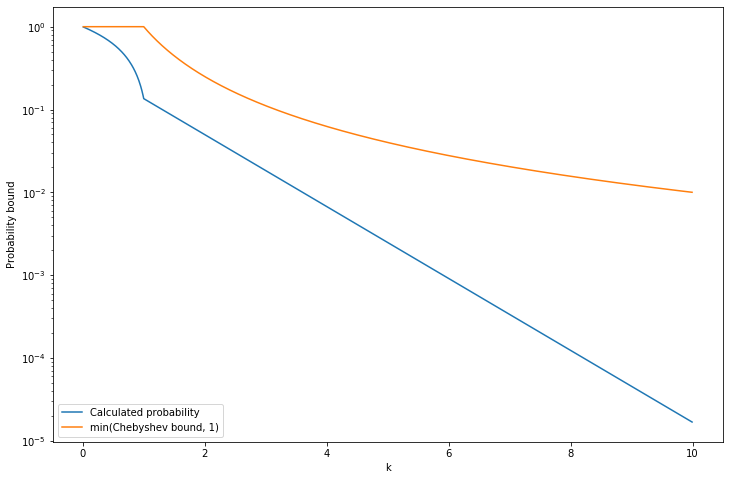
\includegraphics[width=0.9\linewidth,height=0.2\textheight,keepaspectratio]{Figure-05-01}
\end{figure}

\textbf{Exercise 5.6.2}. Let \(X \sim \text{Poisson}(\lambda)\). Use
Chebyshev's inequality to show that
\(\mathbb{P}(X \geq 2\lambda) \leq 1 / \lambda\).

\textbf{Solution}. We have \(\mu_X = \lambda\) and
\(\sigma_X^2 = \lambda\), so Chebyshev's gives us:

\[ \mathbb{P}(|X - \lambda| \geq t) \leq \frac{\lambda}{t^2} \]

If we make \(t = \lambda\), we get

\[ \mathbb{P}(X \geq 2\lambda) = \mathbb{P}(|X - \lambda| \geq \lambda) \leq \frac{1}{\lambda} \]

\textbf{Exercise 5.6.3}. Let
\(X_1, \dots, X_n \sim \text{Bernoulli}(p)\) and
\(\overline{X}_n = n^{-1} \sum_{i=1}^n X_i\). Bound
\(\mathbb{P}(|\overline{X}_n - p| > \epsilon)\) using Chebyshev's
inequality and using Hoeffding's inequality.

Show that, when \(n\) is large, the bound from Hoeffding's inequality is
smaller than the bound from Chebyshev's inequality.

\textbf{Solution}. Note that \(\mathbb{E}(\overline{X}_n) = p\) and
\(\mathbb{V}(\overline{X}_n) = p(1-p) / n\), since
\(n \overline{X}_n \sim \text{Binomial}(n, p)\).

Using Chebyshev's inequality,

\[ \mathbb{P}(|\overline{X}_n - p| \geq \epsilon) \leq \frac{p(1 - p)}{n \epsilon^2} \]

Using Hoeffding's inequality,

\[ \mathbb{P}(|\overline{X}_n - p| > \epsilon) \leq 2e^{-2n\epsilon^2} \]

The bound provided by Hoeffding's inequality is
\(O(e^{-2n\epsilon^2})\), while the bound provided by Chebyshev's
inequality is \(O(n^{-1})\), therefore the bound from Hoeffding's
inequality is smaller for a sufficiently large \(n\).

\textbf{Exercise 5.6.4}. Let
\(X_1, \dots, X_n \sim \text{Bernoulli}(p)\).

\textbf{(a)} Let \(\alpha > 0\) be fixed and define

\[ \epsilon_n = \sqrt{\frac{1}{2n} \log \left( \frac{2}{\alpha}\right)} \]

Let \(\hat{p}_n = n^{-1} \sum_{i=1}^n X_i\). Define
\(C_n = (\hat{p}_n - \epsilon_n, \hat{p}_n + \epsilon_n)\). Use
Hoeffding's inequality to show that

\[ \mathbb{P}(p \in C_n) \geq 1 - \alpha \]

We call \(C_n\) a \emph{\(1 - \alpha\) confidence interval for \(p\)}.
In practice, we truncate the interval so it does not go below 0 or above
1.

\textbf{(b) (Computer Experiment)} Let's examine the properties of this
confidence interval. Let \(\alpha = 0.05\) and \(p = 0.4\). Conduct a
simulation study to see how often the interval contains \(p\) (called
the coverage). Do this for various values of \(n\) between 1 and 10000.
Plot the coverage versus \(n\).

\textbf{(c)} Plot the length of the interval versus \(n\). Suppose we
want the length of the interval to be no more than .05. How large should
\(n\) be?

\textbf{Solution}.

\textbf{(a)} The result is immediate from replacing \(\epsilon_n\) into
Hoeffding's inequality,

\[ \mathbb{P}(|\hat{p}_n - p| > \epsilon_n) \leq 2e^{-2n\epsilon_n^2} = \alpha \]

since \(\mathbb{E}(\hat{p}_n) = p\).

\textbf{(b)}

\begin{python}
import numpy as np
from scipy.stats import bernoulli
from tqdm import tqdm_notebook

alpha = 0.05
p = 0.4

B = 50000
N = 10000

nn = np.arange(1, N + 1)
epsilon_n = np.sqrt((1 / (2 * nn)) * np.log(2 / alpha))

p_hat = np.empty((B, N))
for i in tqdm_notebook(range(B)):
    X = bernoulli.rvs(p, size=N, random_state=i)
    p_hat[i] = np.cumsum(X) / nn

coverage = np.mean((p_hat + epsilon_n >= p) & (p_hat - epsilon_n <= p), axis=0)
\end{python}

\begin{python}
import matplotlib.pyplot as plt

plt.figure(figsize=(12, 8))
plt.plot(nn, coverage)
plt.xlabel('n')
plt.ylabel('Coverage')
plt.show()
\end{python}

\begin{figure}[H]
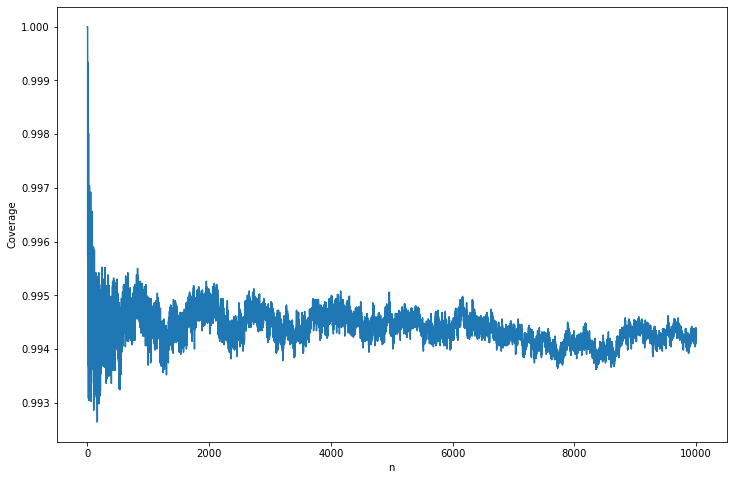
\includegraphics[width=0.9\linewidth,height=0.2\textheight,keepaspectratio]{Figure-05-02}
\end{figure}

\textbf{(c)} The length of the interval is
\(\min \{\hat{p}_n + \epsilon_n, 1 \} - \max \{ \hat{p}_n - \epsilon_n, 0\}\).
As \(\hat{p}_n \rightarrow p\), let's plot the approximation on the
limit case, which is just \(2 \epsilon_n\).

\begin{python}
plt.figure(figsize=(12, 8))
plt.plot(nn, 2 * epsilon_n, label='Interval length')
plt.xlabel('n')
plt.ylabel(r'$2\epsilon_n$')
plt.hlines(.05, xmin=0, xmax=N, color='red', label='Threshold')
plt.yscale('log')
plt.legend(loc='upper right')
plt.show()

selected_n = nn[np.argmax(2 * epsilon_n <= .05)]
print('Smallest n with interval length under .05: %i' % selected_n)
\end{python}

\begin{figure}[H]
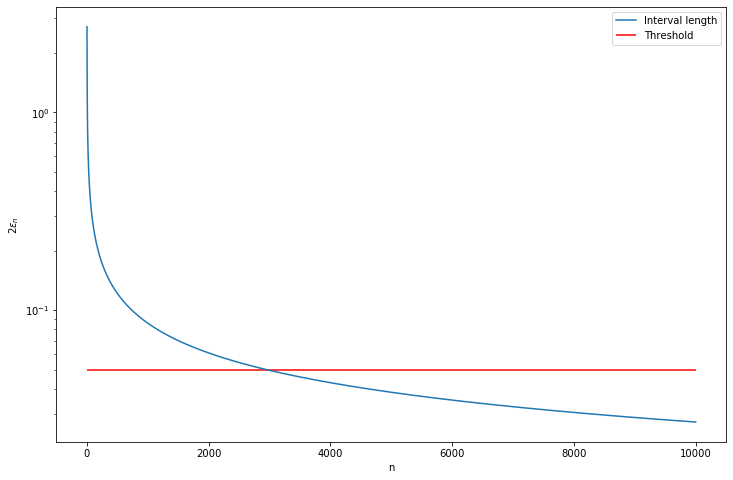
\includegraphics[width=0.9\linewidth,height=0.2\textheight,keepaspectratio]{Figure-05-03}
\end{figure}

\begin{console}
Smallest n with interval length under .05: 2952
\end{console}


% Chapter 6
\section{6. Convergence of Random Variables}\label{convergence-of-random-variables}

\subsection{6.2 Types of convergence}\label{types-of-convergence}

\textbf{\(X_n\) converges to \(X\) in probability}, written
\(X_n \xrightarrow{\text{P}} X\), if, for every \(\epsilon > 0\),:

\[ \mathbb{P}( |X_n - X| > \epsilon ) \rightarrow 0 \]

as \(n \rightarrow \infty\).

\textbf{\(X_n\) converges to \(X\) in distribution}, written
\(X_n \leadsto X\), if

\[ \lim _{n \rightarrow \infty} F_n(t) = F(t) \]

for all \(t\) for which \(F\) is continuous.

\textbf{\(X_n\) converges to \(X\) in quadratic mean}, written
\(X_n \xrightarrow{\text{qm}} X\), if,

\[ \mathbb{E}(X_n - X)^2 \rightarrow 0 \]

as \(n \rightarrow \infty\).

\textbf{Theorem 6.4}. The following relationships hold:

\begin{enumerate}[label={\arabic*.}]
\item
  \(X_n \xrightarrow{\text{qm}} X\) implies that
  \(X_n \xrightarrow{P} X\).
\item
  \(X_n \xrightarrow{\text{P}} X\) implies that \(X_n \leadsto X\).
\item
  if \(X_n \leadsto X\) and if \(\mathbb{P}(X = c) = 1\) for some real
  number \(c\), then \(X_n \xrightarrow{\text{P}} X\).
\end{enumerate}

\textbf{Proof}

\begin{enumerate}[tightlist,label={\arabic*.}]
\item
  Fix \(\epsilon > 0\). Using Chebyshev's inequality,
\end{enumerate}

\[ \mathbb{P}(|X_n - X| > \epsilon) = \mathbb{P}(|X_n - X|^2 < \epsilon^2) \leq \frac{\mathbb{E}|X_n - X|^2}{\epsilon^2} \rightarrow 0 \]

\begin{enumerate}[tightlist,label={\arabic*.}]
\item
  Fix \(\epsilon > 0\) and let \(x\) be a point of continuity of \(F\).
  Then
\end{enumerate}

\begin{align}
F_n(x) & = \mathbb{P}(X_n \leq x) = \mathbb{P}(X_n \leq x, X \leq x + \epsilon) + \mathbb{P}(X_n \leq x, X > x + \epsilon) \\
       & \leq \mathbb{P}(X \leq x + \epsilon) + \mathbb{P}(|X_n - X| > \epsilon) \\
       & = F(x + \epsilon) + \mathbb{P}(|X_n - X| > \epsilon)
\end{align}

Also,

\begin{align}
F(x - \epsilon) & = \mathbb{P}(X \leq x - \epsilon) = \mathbb{P}(X \leq x - \epsilon, X_n \leq x) + \mathbb{P}(X \leq x + \epsilon, X_n > x) \\
                & \leq F_n(x) + \mathbb{P}(|X_n - X| > \epsilon)
\end{align}

Hence,

\[ F(x - \epsilon) - \mathbb{P}(|X_n - X| > \epsilon) \leq F_n(x) \leq F_n(x + \epsilon) + \mathbb{P}(|X_n - X| > \epsilon) \]

Take the limit as \(n \rightarrow \infty\) to conclude that

\[ F(x - \epsilon) \leq \liminf_{n \rightarrow \infty} F_n(x) \leq \limsup_{n \rightarrow \infty} F_n(x) \leq F(x + \epsilon) \]

\begin{enumerate}[tightlist,label={\arabic*.},resume]
\item
  Fix \(\epsilon > 0\). Then,
\end{enumerate}

\begin{align}
\mathbb{P}(|X_n - c| > \epsilon) & = \mathbb{P}(X_n < c - \epsilon) + \mathbb{P}(X_n > c + \epsilon) \\
                                 & \leq \mathbb{P}(X_n \leq c - \epsilon) + \mathbb{P}(X_n > c + \epsilon) \\
                                 & = F_n(c - \epsilon) + 1 - F_n(c + \epsilon) \\
                                 & \rightarrow F(c - \epsilon) + 1 - F(c + \epsilon) \\
                                 & = 0 + 1 - 1 = 0
\end{align}

Now, to show that the reverse implications do not hold:

\paragraph{Convergence in probability does not imply convergence in
quadratic
mean}\label{convergence-in-probability-does-not-imply-convergence-in-quadratic-mean}

Let \(U \sim \text{Unif}(0, 1)\), and let
\(X_n \sim \sqrt{n} I_{(0, 1 / n)}(U)\). Then
\(\mathbb{P}(|X_n| > \epsilon) = \mathbb{P}(\sqrt{n} I_{(0, 1 / n)}(U) > \epsilon) = \mathbb{P}(0 \leq U < 1/n) = 1/n \rightarrow 0\).
Hence, then \(X_n \xrightarrow{\text{P}} 0\). But
\(\mathbb{E}(X_n^2) = n \int_0^{1/n} du = 1\) for all \(n\) so \(X_n\)
does not converge in quadratic mean.

\paragraph{Convergence in distribution does not imply convergence in
probability}\label{convergence-in-distribution-does-not-imply-convergence-in-probability}

Let \(X \sim N(0, 1)\). Let \(X_n = -X\) for \(n = 1, 2, 3, \dots\);
hence \(X_n \sim N(0, 1)\). \(X_n\) has the same distribution as \(X\)
for all \(n\) so, trivially, \(\lim _n F_n(x) \rightarrow F(x)\) for all
\(x\). Therefore, \(X_n \leadsto X\). But
\(\mathbb{P}(|X_n - X| > \epsilon) = \mathbb{P}(|2X| > \epsilon) \neq 0\).
So \(X_n\) does not tend to \(X\) in probability.

\begin{figure}[H]
\centering
\pandocbounded{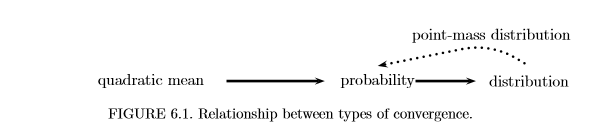
\includegraphics[keepaspectratio]{Figure-06-01}}
\caption{Figure-06-01}
\end{figure}

\textbf{Theorem 6.5} Let \(X_n, X, Y_n, Y\) be random variables. Let
\(g\) be a continuous function. Then:

\begin{enumerate}[tightlist,label={\arabic*.}]
\item
  If \(X_n \xrightarrow{\text{P}} X\) and
  \(Y_n \xrightarrow{\text{P}} Y\), then
  \(X_n + Y_n \xrightarrow{\text{P}} X + Y\).
\item
  If \(X_n \xrightarrow{\text{qm}} X\) and
  \(Y_n \xrightarrow{\text{qm}} Y\), then
  \(X_n + Y_n \xrightarrow{\text{qm}} X + Y\).
\item
  If \(X_n \leadsto X\) and \(Y_n \leadsto c\), then
  \(X_n + Y_n \leadsto X + c\).
\item
  If \(X_n \xrightarrow{\text{P}} X\) and
  \(Y_n \xrightarrow{\text{P}} Y\), then
  \(X_n Y_n \xrightarrow{\text{P}} XY\).
\item
  If \(X_n \leadsto X\) and \(Y_n \leadsto c\), then
  \(X_n Y_n \leadsto cX\).
\item
  If \(X_n \xrightarrow{\text{P}} X\) then
  \(g(X_n) \xrightarrow{\text{P}} g(X)\) .
\item
  If \(X_n \leadsto X\) then \(g(X_n) \leadsto g(X)\).
\end{enumerate}

\subsection{6.3 The Law of Large
Numbers}\label{the-law-of-large-numbers}

\textbf{Theorem 6.6 (The Weak Law of Large Numbers (WLLN))}. If
\(X_1, X_2, \dots, X_n\) are IID, then
\(\overline{X}_n \xrightarrow{\text{P}} \mu\).

\textbf{Proof}: Assume that \(\sigma < \infty\). This is not necessary
but it simplifies the proof. Using Chebyshev's inequality,

\[ \mathbb{P}(|\overline{X}_n - \mu| > \epsilon) \leq \frac{\mathbb{E}(|\overline{X}_n - \mu|^2)}{\epsilon^2} = \frac{\mathbb{V}(\overline{X}_n)}{\epsilon^2} = \frac{\sigma^2}{n \epsilon^2} \]

which tends to 0 as \(n \rightarrow \infty\).

\subsection{6.4 The Central Limit
Theorem}\label{the-central-limit-theorem}

\textbf{Theorem 6.8 (The Central Limit Theorem (CLT))}. Let
\(X_1, X_2, \dots, X_n\) be IID with mean \(\mu\) and variance
\(\sigma^2\). Let \(\overline{X}_n = n^{-1}\sum_{i=1}^n X_i\). Then

\[ Z_n \equiv \frac{\sqrt{n} \left( \overline{X}_n - \mu \right)}{\sigma} \leadsto Z \]

where \(Z \sim N(0, 1)\). In other words,

\[ \lim _{n \rightarrow \infty} \mathbb{P}(Z_n \leq z) = \Phi(z) = \int _{-\infty} ^z \frac{1}{\sqrt{2 \pi}} e^{-x^2/2}dx\]

In addition to \(Z_n \leadsto N(0, 1)\), there are several forms of
notation to denote the fact that the distribution of \(Z_n\) is
converging to a Normal. They all mean the same thing. Here they are:

\begin{align}
Z_n                                           & \approx N(0, 1) \\
\overline{X}_n                                & \approx N\left( \mu, \frac{\sigma^2}{n} \right)  \\
\overline{X}_n - \mu                          & \approx N\left( 0,   \frac{\sigma^2}{n} \right)  \\
\sqrt{n}(\overline{X}_n - \mu)                & \approx N\left( 0, \sigma^2 \right)              \\
\frac{\sqrt{n}(\overline{X}_n - \mu)}{\sigma} & \approx N(0, 1)
\end{align}

The central limit theorem tells us that
\(Z_n = \sqrt{n}(\overline{X}_n - \mu)/\sigma\) is approximately
\(N(0, 1)\). However, we rarely know \(\sigma\). We can estimate
\(\sigma^2\) from \(X_1, X_2, \dots, X_n\) by

\[ S_n^2 = \frac{1}{n - 1} \sum_{i=1}^n ( X_i - \overline{X}_n )^2 \]

This raises the following question: if we replace \(\sigma\) with
\(S_n\) is the central limit theorem still true? The answer is yes.

\textbf{Theorem 6.10}. Assume the same conditions as the CLT. Then,

\[ \frac{\sqrt{n} \left(\overline{X}_n - \mu \right)}{S_n} \leadsto N(0, 1)\]

You might wonder how accurate the normal approximation is. The answer is
given by the Berry-Essèen theorem.

\textbf{Theorem 6.11 (Berry-Essèen)}. Suppose that
\(\mathbb{E}|X_1|^3 < \infty\). Then

\[ \sup _z |\mathbb{P}(Z_n \leq z) - \Phi(z)| \leq \frac{33}{4} \frac{\mathbb{E}|X_1 - \mu|^3}{\sqrt{n}\sigma^3} \]

There is also a multivariate version of the central limit theorem.

\textbf{Theorem 6.12 (Multivariate central limit theorem)}. Let
\(X_1, \dots, X_n\) be IID random vectors where

\[ X_i = \begin{pmatrix} X_{1i} \\ X_{2i} \\ \vdots \\ X_{ki} \end{pmatrix}\]

with mean

\[ \mu 
= \begin{pmatrix} \mu_1 \\ \mu_2 \\ \vdots \\ \mu_k \end{pmatrix} 
= \begin{pmatrix} \mathbb{E}(X_{1i}) \\ \mathbb{E}(X_{2i}) \\ \vdots \\ \mathbb{E}(X_{ki}) \end{pmatrix} \]

and variance matrix \(\Sigma\). Let

\[ \overline{X} = \begin{pmatrix} \overline{X}_1 \\ \overline{X}_2 \\ \vdots \\ \overline{X}_k \end{pmatrix}\]

where \$\overline{X}\emph{r = n\^{}\{-1\} \sum}\{i=1\}\^{}n X\_\{ri\}
\$. Then,

\[ \sqrt{n} (\overline{X} - \mu) \leadsto N(0, \Sigma) \]

\subsection{6.5 The Delta Method}\label{the-delta-method}

\textbf{Theorem 6.13 (The Delta Method)}. Suppose that

\[ \frac{\sqrt{n}(Y_n - \mu)}{\sigma} \leadsto N(0, 1)\]

and that \(g\) is a differentiable function such that \(g'(u) \neq 0\).
Then

\[ \frac{\sqrt{n}(g(Y_n) - g(u))}{|g'(u)| \sigma} \leadsto N(0, 1)\]

In other words,

\[ Y_n \approx N \left( \mu, \frac{\sigma^2}{n} \right) \Rightarrow g(Y_n) \approx N \left( g(\mu), (g'(\mu))^2 \frac{\sigma^2}{n} \right) \]

\textbf{Theorem 6.15 (The Multivariate Delta method)}. Suppose that
\(Y_n = (Y_{n1}, \dots, Y_{nk})\) is a sequence of random vectors such
that

\[ \sqrt{n}(Y_n - \mu) \leadsto N(0, \Sigma) \]

Let \(g : \mathbb{R}^k \rightarrow \mathbb{R}\) and let

\[ \nabla g = \begin{pmatrix} \frac{\partial g}{\partial y_1} \\ \vdots \\  \frac{\partial g}{\partial y_k} \end{pmatrix} \]

Let \(\nabla_\mu\) denote \(\nabla g(y)\) evaluated at \(y = \mu\) and
assume that the elements of \(\nabla_\mu\) are non-zero. Then

\[ \sqrt{n}(g(Y_n) - g(\mu)) \leadsto N(0, \nabla_\mu^T \Sigma \nabla_\mu) \]

\subsection{6.6 Technical appendix}\label{technical-appendix}

\textbf{\(X_n\) converges to \(X\) almost surely}, written
\(X_n \xrightarrow{\text{as}} X\), if

\[ \mathbb{P}(\{s : X_n(s) \rightarrow X(s)\}) = 1 \]

\textbf{\(X_n\) converges to \(X\) in \(L_1\)}, written
\(X_n \xrightarrow{L_1} X\), if

\[ \mathbb{E} |X_n - X| \rightarrow 0 \]

\textbf{Theorem 6.17}. Let \(X_n\) and \(X\) be random variables. Then:

\begin{enumerate}[tightlist,label={\arabic*.}]
\item
  \(X_n \xrightarrow{\text{as}} X\) implies that
  \(X_n \xrightarrow{\text{P}} X\).
\item
  \(X_n \xrightarrow{\text{qm}} X\) implies that
  \(X_n \xrightarrow{L_1} X\).
\item
  \(X_n \xrightarrow{L_1} X\) implies that
  \(X_n \xrightarrow{\text{P}} X\).
\end{enumerate}

The weak law of large numbers says that \(\overline{X}_n\) converges to
\(\mathbb{E} X\) in probability. The strong law asserts that this is
also true almost surely.

\textbf{Theorem 6.18 (The strong law of large numbers)}. Let
\(X_1, X_2, \dots, X_n\) be IID. If \(\mu = \mathbb{E}|X_1| < \infty\)
then \(\overline{X}_n \xrightarrow{\text{as}} \mu\).

A sequence is \textbf{asymptotically uniformly integrable} if

\[ \lim _{M \rightarrow \infty} \limsup _{n \rightarrow \infty} \mathbb{E} ( |X_n| I(|X_n| > M) ) = 0 \]

If \(X_n \xrightarrow{\text{P}} b\) and \(X_n\) is asymptotically
uniformly integrable, then \(\mathbb{E}(X_n) \rightarrow b\).

The \textbf{moment generating function} of a random variable \(X\) is

\[\psi_X(t) = \mathbb{E}(e^{tX}) = \int_u e^{tu} f_X(u) du\]

\textbf{Lemma 6.19}. Let \(Z_1, Z_2, \dots, Z_n\) be a sequence of
random variables. Let \(\psi_n\) be the mgf of \(Z_n\). Let \(Z\) be
another random variable and denote its mgf by \(\psi\). If
\(\psi_n(t) \rightarrow \psi(t)\) for all \(t\) in some open interval
around 0, then \(Z_n \leadsto Z\).

\paragraph{Proof of the Central Limit
Theorem}\label{proof-of-the-central-limit-theorem}

Let \(Y_i = (X_i - \mu) / \sigma\). Then, \(Z_n = n^{-1/2} \sum_i Y_i\).
Let \(\psi(t)\) be the mgf of \(Y_i\). The mgf of \(\sum_i Y_i\) is
\((\psi(t))^n\) and the mgf of \(Z_n\) is
\([\psi(t / \sqrt{n})]^n \equiv \xi_n(t)\).

Now \(\psi'(0) = \mathbb{E}(Y_1) = 0\) and
\(\psi''(0) = \mathbb{E}(Y_1^2) = \mathbb{V}(Y_1) = 1\). So,

\begin{align}
\psi(t) & = \psi(0) + t \psi'(0) + \frac{t^2}{2!} \psi''(0) + \frac{t^3}{3!} \psi'''(0) + \dots \\
        & = 1 + 0 + \frac{t^2}{2} +  \frac{t^3}{3!} \psi'''(0) + \ldots \\
        & = 1 + \frac{t^2}{2} +  \frac{t^3}{3!} \psi'''(0) + \ldots
\end{align}

Now,

\begin{align}
\xi_n(t) & = \left[ \psi \left( \frac{t}{\sqrt{n}} \right) \right] ^n \\
         & = \left[  1 + \frac{t^2}{2n} +  \frac{t^3}{3!n^{3/2}} \psi'''(0) + \ldots \right] ^n \\
         & = \left[  1 + \frac{\frac{t^2}{2} +  \frac{t^3}{3!n^{1/2}} \psi'''(0) + \ldots}{n} \right] ^n \\
         & \rightarrow e^{t^2/2}
\end{align}

which is the mgf of \(N(0, 1)\). The resolt follows from the previous
theorem. In the last step we used the fact that, if
\(a_n \rightarrow a\), then

\[ \left( 1 + \frac{a_n}{n} \right) ^n \rightarrow e^a \]

\subsection{6.8 Exercises}\label{exercises}

\textbf{Exercise 6.8.1.} Let \(X_1, \dots, X_n\) be iid with finite mean
\(\mu = \mathbb{E}(X_i)\) and finite variance
\(\sigma^2 = \mathbb{V}(X_i)\). Let \(\overline{X}_n\) be the sample
mean and let \(S_n^2\) be the sample variance.

\textbf{(a)} Show that \(\mathbb{E}(S_n^2) = \sigma^2\).

\textbf{Solution}:

\(S_n^2\) is the sample variance, that is, \$ S\_n\^{}2 =
(n-1)\^{}\{-1\} \sum\_\{i=1\}\^{}n ( X\_i - \overline{X}\_n)\^{}2 \$.
Therefore:

\begin{align}
\mathbb{E}[S_n^2] & = \mathbb{E}\left[ \frac {1}{n-1} \sum_{i=1}^n \left(X_i - \overline{X}_n \right)^2 \right] \\
& = \frac {1}{n-1} \mathbb{E} \left( \sum_{i=1}^n X_i^2 - 2 \overline{X}_n \sum_{i=1}^n X_i + \sum_{i=1}^n \overline{X}_n^2 \right) \\
& = \frac {1}{n-1} \mathbb{E} \left( \sum_{i=1}^n X_i^2 - 2 n \overline{X}_n^2 + n \overline{X}_n^2 \right) \\
& = \frac {n}{n-1} \left[ \mathbb{E} (X_i^2) - \mathbb{E} \overline{X}_n^2 \right] \\
& = \frac {n}{n-1} \left[ \left( \mu^2+\sigma^2 \right) - \left( \mu^2 + \frac {\sigma^2}{n} \right) \right] \\
& = \sigma^2
\end{align}

\textbf{(b)} Show that \(S_n^2 \xrightarrow{\text{P}} \sigma^2\).

Hint: show that
\(S_n^2 = c_n n^{-1} \sum_{i=1}^n X_i^2 - d_n \overline{X}_n^2\) where
\(c_n \rightarrow 1\) and \(d_n \rightarrow 1\). Apply the law of large
numbers to \(n^{-1}\sum_{i=1}^n X_i^2\) and to \(\overline{X}_n\). Then
use part (e) of Theorem 6.5.

\textbf{Solution}:

Similar to derivation in \textbf{(a)} we have:

\begin{align}
S_n^2 & = \frac {1}{n-1} \left( \sum_{i=1}^n X_i^2 - n \overline{X}_n^2 \right) \\
& = \frac{n}{n-1} \frac{1}{n} \sum_{i=1}^n X_i^2 - \frac{n}{n-1} \overline{X}_n^2 
\end{align}

where \(c_n = d_n = \frac{n}{n-1} \rightarrow 1\).

Applying the law of large numbers to \(X_i^2\):

\[ n^{-1} \sum_{i=1}^n X_i^2 \xrightarrow{\text{P}} \mathbb{E}(X_i^2) = \sigma^2 + \mu^2\]

\[ \overline{X}_n \xrightarrow{\text{P}} \mathbb{E}(X_i) = \mu \Rightarrow \overline{X}_n^2 \xrightarrow{\text{P}} \mu^2 \]

Therefore, from theorem 6.5.e, \$ S\_n\^{}2 = c\_n n\^{}\{-1\}
\sum\_\{i=1\}\^{}n X\_i\^{}2 - d\_n \overline{X}\_n\^{}2
\xrightarrow{\text{P}} \sigma\^{}2 + \mu\^{}2 - \mu\^{}2 =
\sigma\^{}2\$.

\textbf{Exercise 6.8.2.} Let \(X_1, X_2, \dots, X_n\) be a sequence of
random variables. Show that \(X_n \xrightarrow{\text{qm}} b\) if and
only if

\[
\begin{equation}
\lim_{n \rightarrow \infty} \mathbb{E}(X_n) = b
\quad\mathrm{and}\quad 
\lim_{n \rightarrow \infty} \mathbb{V}(X_n) = 0
\end{equation}
\]

\textbf{Solution}:

\(X_n \xrightarrow{\text{qm}} b\) id equivalent to:

\begin{align}
\mathbb{E}[(X_n - b)^2]           & \rightarrow 0 \\
\mathbb{E}[X_n^2 - 2b X_n + b^2]  & \rightarrow 0 \\
\mathbb{E}[X_n^2] - 2b \mathbb{E}[X_n] + b^2 & \rightarrow 0 \\
\mathbb{E}[X_n^2] - 2b \mathbb{E}[X_n] + b^2 & \rightarrow 0 \\
\mathbb{V}[X_n] + (\mathbb{E}[X_n])^2 - 2b \mathbb{E}[X_n] + b^2  & \rightarrow 0
\end{align}

If \(\lim_{n \rightarrow \infty} \mathbb{V}[X_n] = 0\) and
\(\lim_{n \rightarrow \infty} \mathbb{E}[X_n] = b\), then

\begin{align}
& \lim_{n \rightarrow \infty} \mathbb{E}[(X_n - b)^2] = \\
& = \lim_{n \rightarrow \infty} \mathbb{V}[X_n] + (\mathbb{E}[X_n])^2 - 2b \mathbb{E}[X_n] + b^2 \\
& = \lim_{n \rightarrow \infty} \mathbb{V}[X_n] + (\lim_{n \rightarrow \infty} \mathbb{E}[X_n])^2 - 2b \lim_{n \rightarrow \infty} \mathbb{E}[X_n] + b^2 \\
&= 0 + b^2 - 2b^2 + b^2 \\
&= 0
\end{align}

On the other direction, if \(X_n \xrightarrow{\text{qm}} b\), then

\begin{align}
\lim_{n \rightarrow \infty} \mathbb{V}[X_n] + (\lim_{n \rightarrow \infty} \mathbb{E}[X_n])^2 - 2b \lim_{n \rightarrow \infty} \mathbb{E}[X_n] + b^2 &= 0 \\
\lim_{n \rightarrow \infty} \mathbb{V}[X_n] + (\lim_{n \rightarrow \infty} \mathbb{E}[X_n] - b)^2 &= 0 \\
\lim_{n \rightarrow \infty} \mathbb{V}[X_n - b] + \lim_{n \rightarrow \infty}  (\mathbb{E}[X_n - b])^2 &= 0
\end{align}

Since both terms inside the limits are non-negative, the limits
themselves are non-negative. Two non-negative values add up to 0, so
they must both be zero, and so we have:

\[
\begin{equation}
\lim_{n \rightarrow \infty} \mathbb{E}(Y_n) = 0
\quad\mathrm{and}\quad 
\lim_{n \rightarrow \infty} \mathbb{V}(Y_n) = 0
\end{equation}
\]

or, equivalently,

\[
\begin{equation}
\lim_{n \rightarrow \infty} \mathbb{E}(X_n) = b
\quad\mathrm{and}\quad 
\lim_{n \rightarrow \infty} \mathbb{V}(X_n) = 0
\end{equation}
\]

\textbf{Exercise 6.8.3}. Let \(X_1, X_2, \dots, X_n\) be iid and let
\(\mu = \mathbb{E}(X_i)\). Suppose that variance is finite. Show that
\(\overline{X}_n \xrightarrow{\text{qm}} \mu\).

\textbf{Solution}.

Let \(Y_i = X_i - \mu\). It has variance \(\sigma_Y = \sigma\) and mean
\(\mu_Y = 0\). We have:

\begin{align}
& \mathbb{E}[(\overline{X}_n - \mu)^2] = \\
& = \mathbb{E}\left[\left(\frac{1}{n} \sum_{i=1}^n (X_i - \mu) \right)^2\right] \\
& = \frac{1}{n^2} \mathbb{E} \left[ \left(\sum_{i=1}^n Y_i \right)^2 \right] \\
& = \frac{1}{n^2} \left( \sum_{i=1}^n \mathbb{E}[Y_i^2] - \sum_{i=1}^n \sum_{j=1, j \neq i}^n \mathbb{E}[Y_i Y_j] \right) \\
& = \frac{1}{n} \left( (\sigma_Y^2 + \mu_Y^2) - (n-1) \mu_Y^2 \right) \\
& = \frac{\sigma}{n}
\end{align}

Therefore,
\(\lim _{n \rightarrow \infty} \mathbb{E}[(\overline{X}_n - \mu)^2] = \lim _{n \rightarrow \infty} \sigma / n = 0\),
and so \(\overline{X}_n \xrightarrow{\text{qm}} \mu\).

\textbf{Exercise 6.8.4}. Let \(X_1, X_2, \dots\) be a sequence of random
variables such that

\[
\begin{equation}
\mathbb{P}\left(X_n = \frac{1}{n}\right) = 1 - \frac{1}{n^2}
\quad\mathrm{and}\quad 
\mathbb{P}\left(X_n = n\right) = \frac{1}{n^2}
\end{equation}
\]

Does \(X_n\) converge in probability? Doex \(X_n\) converge in quadratic
mean?

\textbf{Solution}.

For any distribution \(X\), we have:

\begin{align}
& \mathbb{P}( |X_n - X| > \epsilon ) = \\
&= \mathbb{P}\left( |X_n - X| > \epsilon \;\middle|\; X_n = \frac{1}{n} \right)\mathbb{P}\left(X_n = \frac{1}{n}\right)
  + \mathbb{P}\left( |X_n - X| > \epsilon \;\middle|\; X_n = n \right)\mathbb{P}\left(X_n = n\right) \\
&= \mathbb{P}\left( \middle|\frac{1}{n} - X\middle|\; > \epsilon \right)\left(1 - \frac{1}{n^2} \right)
  + \mathbb{P}\left( |n - X| > \epsilon \right)\frac{1}{n^2}
\end{align}

Looking at the limit as \(n \rightarrow \infty\),

\begin{align}
& \lim _{n \rightarrow \infty} \mathbb{P}( |X_n - X| > \epsilon ) = \\
& = \lim _{n \rightarrow \infty} \mathbb{P}\left( \middle|\frac{1}{n} - X\middle|\; > \epsilon \right)\left(1 - \frac{1}{n^2} \right)
  + \lim _{n \rightarrow \infty} \mathbb{P}\left( |n - X| > \epsilon \right)\frac{1}{n^2} \\
& = \lim _{n \rightarrow \infty} \mathbb{P}\left( |X| > \epsilon \right)
\end{align}

If we set \(X = 0\), the limit above will be zero for any positive
\(\epsilon\) -- so we have \(X_n \xrightarrow{\text{P}} 0\).

Now, for any quadratic mean potential convergence, we have:

\begin{align}
& \mathbb{E}\left[(X_n - X)^2\right] = \\
& = \mathbb{E}\left[(X_n - X)^2 \bigg| X_n = \frac{1}{n} \right] \mathbb{P}\left(X_n = \frac{1}{n}\right)
   + \mathbb{E}\left[(X_n - X)^2 \big| X_n = n \right] \mathbb{P}\left(X_n = n\right) \\
& = \mathbb{E}\left[\left(X - \frac{1}{n}\right)^2  \right] \left(1 - \frac{1}{n^2}\right)
   + \mathbb{E}\left[(X - n)^2  \right] \frac{1}{n^2} \\
& = \mathbb{E}\left[X^2 - 2Xn^{-1} + n^{-2} \right] \left(1 - \frac{1}{n^2}\right)
   + \mathbb{E}\left[X^2 - 2Xn + n^2 \right] \frac{1}{n^2} \\
& = \mathbb{E}\left[X^2\right] + \mathbb{E}\left[X\right] \left(\frac{-2}{n} \left(1 - \frac{1}{n^2} \right) -\frac{2}{n}\right) + \frac{1}{n^2} \left(1 - \frac{1}{n^2} \right) + 1 \\
& = \mathbb{E}\left[X^2\right] - \mathbb{E}\left[X\right] \frac{2}{n} \left( 2 + \frac{1}{n^2} \right) + \frac{1}{n^2} \left(1 - \frac{1}{n^2} \right) + 1
\end{align}

Taking the limit as \(n \rightarrow \infty\),

\begin{align}
& \lim _{n \rightarrow \infty} \mathbb{E}\left[(X_n - X)^2\right] = \\
& = 1 + \lim _{n \rightarrow \infty} \mathbb{E}\left[X^2\right] \\
& = 1 + \mathbb{E}\left[X^2\right] \\
& \geq 1
\end{align}

so there is no distribution \(X\) for which this value is 0, and so
there is no quadratic mean convergence.

\textbf{Exercise 6.8.5}. Let
\(X_1, \dots, X_n \sim \text{Bernoulli}(p)\). Prove that

\[
\begin{equation}
\frac{1}{n} \sum_{i=1}^n X_i^2 \xrightarrow{\text{P}} p
\quad\mathrm{and}\quad 
\frac{1}{n} \sum_{i=1}^n X_i^2 \xrightarrow{\text{qm}} p
\end{equation}
\]

\textbf{Solution}.

Given that quadratic mean convergence implies probability convergence,
we only need to prove the second proposition.

Let \(Y_i = X_i^2 - p\). Then:

\begin{align}
\mathbb{E}[Y_i] & = \\
& = \mathbb{E}[X_i^2] - p \\
& = \mathbb{V}[X_i] + \mathbb{E}[X_i]^2 - p \\
& = p(1-p) + p^2 - p \\
& = 0 \\
\mathbb{E}[Y_i^2] & = \\
& = \mathbb{V}[Y_i] + \mathbb{E}[Y_i]^2 \\
& = \mathbb{V}[X_i^2 - p] + 0^2 \\
& = \mathbb{V}[X_i^2] + 0^2 \\
& = \mathbb{V}[X_i]\\
& = p(1-p) \\
\mathbb{E}[Y_i Y_j] & = \text{(for independent variables)}\\
& = \mathbb{E}[Y_i] \mathbb{E}[Y_j] \\
& = 0
\end{align}

\begin{align}
& \mathbb{E}\left[\left(\left(\frac{1}{n} \sum_{i=1}^n X_i^2\right) - p\right)^2\right] = \\
& = \mathbb{E}\left[\left(\frac{1}{n} \sum_{i=1}^n \left(X_i^2 - p\right)\right)^2\right] \\
& = \frac{1}{n^2} \mathbb{E}\left[\left(\sum_{i=1}^n Y_i\right)^2\right] \\
& = \frac{1}{n^2} \mathbb{E}\left[\sum_{i=1}^n Y_i^2 - \sum_{i=1}^n \sum_{j=1, j \neq i}^n Y_i Y_j\right] \\
& = \frac{1}{n^2} \left( \sum_{i=1}^n \mathbb{E}\left[Y_i^2\right] - \sum_{i=1}^n \sum_{j=1, j \neq i}^n \mathbb{E}\left[ Y_i Y_j \right] \right) \\
& = \frac{p(1-p)}{n}
\end{align}

So, as \(n \rightarrow \infty\), this expectation goes to 0, and we have
quadratic mean convergence.

\textbf{Exercise 6.8.6}. Suppose that the height of men has mean 68
inches and standard deviation 4 inches. We draw 100 men at random. Find
(approximately) the probability that the average height of men in our
sample will be at least 68 inches.

\textbf{Solution}.

We assume all men's heights are measurements from iid variables \(X_i\)
with mean \(\mu = 68\) and variance \(\sigma^2 = 16\).

We need to approximate \(\mathbb{P}(\overline{X}_{100} > \mu)\). But by
the central limit theorem,

\[ \overline{X}_n \approx N\left(\mu, \frac{\sigma^2}{n}\right) \]

so this probability will be approximately
\[\mathbb{P}\left(\frac{\sqrt{n}(\overline{X}_n - \mu)}{\sigma} \geq \frac{\sqrt{n}(\mu- \mu)}{\sigma}\right) = \mathbb{P}\left(\frac{\sqrt{n}(\overline{X}_n - \mu)}{\sigma} \geq 0 \right) = P(Z \geq 0) = \frac{1}{2}\]

\textbf{Exercise 6.8.7}. Let \(\lambda_n = 1/n\) for
\(n = 1, 2, \dots\). Let \(X_n \sim \text{Poisson}(\lambda_n)\).

\textbf{(a)} Show that \(X_n \xrightarrow{\text{P}} 0\).

\textbf{Solution}.

\[
\mathbb{E}(X_n^2) = \mathbb{V}(X_n) + \mathbb{E}(X_n)^2
= \lambda_n^2 + \lambda_n^2 = 2 \lambda_n^2 = 2/n^2
\]

This quantity goes to zero as \(n \rightarrow \infty\), so we have
\(X_n \xrightarrow{\text{qm}} 0\), which implies
\(X_n \xrightarrow{\text{P}} 0\).

\textbf{(b)} Let \(Y_n = n X_n\). Show that
\(Y_n \xrightarrow{\text{P}} 0\).

\textbf{Solution}. Immediate by applying theorem 6.5 item 6. Or
alternatively:

\[
\mathbb{E}(Y_n^2) = \mathbb{V}(Y_n) + \mathbb{E}(Y_n)^2
= n^2 \lambda_n^2 + n^2\lambda_n^2 = 2 n^2 \lambda_n^2 = 2
\]

so we \emph{don't} have a straightforward quadratic mean convergence on
\(Y_n\).

We \emph{don't} have a straightforward \(L_1\) convergence either:

\[\mathbb{E}(|Y_n|) = \mathbb{E}(Y_n) = n \lambda_n = 1\]

However, we can show that \(Y_n \leadsto 0\):

\[\lim _{n \rightarrow \infty} F_{Y_n}(t) = \lim _{n \rightarrow \infty} F_{Y_1}(t / n) = \lim _{n \rightarrow \infty} F_{Y_1}(t / n) = 0 \]

as, when \(n \rightarrow \infty\), the portion of the CDF in the
positive neighborhood of 0 shrinks to \(F_{Y_1}(0) = 0\).

We also have a point mass distribution on our target distribution
\(Y_\infty = 0\): probability of 1 in point 0, and 0 everywhere else.

Therefore, from theorem 6.4 item c, we have
\(Y_n \xrightarrow{\text{P}} 0\).

\textbf{Exercise 6.8.8}. Suppose we have a computer program consisting
of \(n = 100\) pages of code. Let \(X_i\) be the number of errors in the
\(i\)-th page of code. Suppose that the \(X_i\)'s are Poisson with mean
1 and that they are independent. Let \(Y = \sum_{i=1}^n X_i\) be the
total number of errors. Use the central limit theorem to approximate
\(\mathbb{P}(Y < 90)\).

\textbf{Solution}. We have \(Y = n \overline{X}_n\), the total being
\(n\) times the sample mean. We need to approximate:

We need to approximate \(\mathbb{P}(\overline{X}_{100} < 0.9)\). But by
the central limit theorem,

\[ \overline{X}_n \approx N\left(\mu, \frac{\sigma^2}{n}\right) \]

so this probability will be approximately \[
\mathbb{P}\left(\frac{\sqrt{n}(\overline{X}_n - \mu)}{\sigma} < \frac{\sqrt{100}(0.9 - 1)}{0.1}\right) 
= \mathbb{P}\left(\frac{\sqrt{n}(\overline{X}_n - \mu)}{\sigma} < -10 \right) 
= P(Z < -10)\]

\textbf{Exercise 6.8.9}. Suppose that
\(\mathbb{P}(X = 1) = \mathbb{P}(X = -1) = 1/2\). Define

\[
\begin{equation}
  X_n =
    \begin{cases}
      X   & \text{with probability } 1 - \frac{1}{n}\\
      e^n & \text{with probability } \frac{1}{n}
    \end{cases}       
\end{equation}
\]

Does \(X_n\) converge to \(X\) in probability? Does \(X_n\) converge to
\(X\) in distribution? Does \(\mathbb{E}(X - X_n)^2\) converge to 0?

\textbf{Solution}.

For any potential quadratic mean convergence, we'd have:

\begin{align}
&\mathbb{E}(X - X_n)^2 = \\
& = \left(\mathbb{E}(X - X_n \middle| X_n = X)\mathbb{P}(X_n = X) + \mathbb{E}(X - X_n \middle| X_n = e^n)\mathbb{P}(X_n = e^n) \right)^2 \\
& = \left(\mathbb{E}(0)\left(1 - \frac{1}{n} \right) + \mathbb{E}(X - e^n)\frac{1}{n} \right)^2 \\
& = \frac{1}{n^2} \mathbb{E}(X - e^n)^2 \\
& = \frac{1}{n^2} \left( \mathbb{E}(X) - e^n  \right)^2 \\
& = \frac{e^{2n}}{n^2}
\end{align}

which does not converge to 0, so we do not have quadratic mean
convergence.

For any potential distribution convergence, \(X_n\) has a point mass
distribution, and we can write its CDF \(F_{X_n}\) explicitly as:

\[
\begin{equation}
  F_{X_n}(t) =
    \begin{cases}
      0   & \text{if } t < -1 \\
      \frac{1}{2} \left(1 - \frac{1}{n}\right) & \text{if } -1 \leq t < 1 \\
      1 - \frac{1}{n} & \text{if } 1 \leq t < e^n \\
      1 & \text{if } e^n \leq t
    \end{cases}       
\end{equation}
\]

On the other hand, the CDF \(F_X\) of the target distribution \(X\) is:

\[
\begin{equation}
  F_X(t) =
    \begin{cases}
      0   & \text{if } t < -1 \\
      \frac{1}{2} & \text{if } -1 \leq t < 1 \\
      1 & \text{if } 1 \leq t
    \end{cases}       
\end{equation}
\]

We then have:

\[
\begin{equation}
  F_X(t) - F_{X_n}(t) =
    \begin{cases}
      0   & \text{if } t < -1 \\
      \frac{1}{2n} & \text{if } -1 \leq t < 1 \\
      \frac{1}{n} & \text{if } 1 \leq t < e^n \\
      0 & \text{if } e^n \leq t
    \end{cases}       
\end{equation}
\]

so \(0 \leq F_X(t) - F_{X_n}(t) \leq 1/n\), which goes to 0 as
\(n \rightarrow \infty\). Therefore
\(\lim _{n \rightarrow \infty} F_{X_n}(t) = F_X(t)\), or
\(X_n \leadsto X\).

Distribution convergence implies probability convergence, so we also
have probability convergence, \(X_n \xrightarrow{\text{P}} X\).

\textbf{Exercise 6.8.10}. Let \(Z \sim N(0, 1)\). Let \(t > 0\).

\textbf{(a)} Show that, for any \(k > 0\),

\[\mathbb{P}(|Z| > t) \leq \frac{\mathbb{E}|Z|^k}{t^k}\]

\textbf{Solution}.

\$\mathbb{P} (\textbar Z\textbar{} \textgreater{} t) = \mathbb{P}
(\textbar Z\textbar\^{}k \textgreater{} t\^{}k) \$ for any \(k > 0\).
Apply Markov's Inequality by letting \(X = |Z|^k\) the result is
immediate. Or alternatively:

We have:

\begin{align}
&\mathbb{E}|Z|^k = \\
&= \int _{-\infty}^{\infty} |z|^{k+1}\left( \frac{1}{\sqrt{2\pi}} e^{-z^2/2} \right) dz \\
&= \int _{-\infty}^{0} (-z)^{k+1}\left( \frac{1}{\sqrt{2\pi}} e^{-z^2/2} \right) dz
  + \int _{0}^{\infty} z^{k+1}\left( \frac{1}{\sqrt{2\pi}} e^{-z^2/2} \right) dz \\
&=  \left\{ \frac{2}{\pi} \right\}^{1/2} \int _{0}^{\infty} z^k \left( z e^{-z^2/2} \right) dz
\end{align}

For t \textgreater{} 0,

\begin{align}
&\mathbb{P}(|Z| > t) = \\
&= 2 \int _t^{\infty} z\left( \frac{1}{\sqrt{2\pi}} e^{-z^2/2} \right) dz \\
&= \left\{ \frac{2}{\pi} \right\}^{1/2} \int _t^{\infty} z e^{-z^2/2} dz
\end{align}

Now we need to prove:

\[\int _t^{\infty} z e^{-z^2/2} dz \leq \frac{1}{t^k}\int _{0}^{\infty} z^k \left( z e^{-z^2/2} \right) dz \]

As the integrands are always positive, we can prove the stronger
statement that, for \(k \geq 0\):

\begin{align}
\int _t^{\infty} z e^{-z^2/2} dz & \leq \frac{1}{t^k}\int _{t}^{\infty} z^k \left( z e^{-z^2/2} \right) dz  \\
t^k \int _t^{\infty} z e^{-z^2/2} dz & \leq \int _{t}^{\infty} z^k \left( z e^{-z^2/2} \right) dz  \\
0 & \leq \int _{t}^{\infty} (z^k - t^k) \left( z e^{-z^2/2} \right) dz  \\
\end{align}

But that's true, since \((z^k - t^k) (z e^{-z^2/2}) \geq 0\) whenever
\(z \geq t\). So the given statement follows.

\textbf{(b) (Mill's inequality)} Show that

\[\mathbb{P}(|Z| > t) \leq \left\{ \frac{2}{\pi} \right\}^{1/2} \frac{e^{-t^2/2}}{t}\]

Hint. Note that \(\mathbb{P}(|Z| > t) = 2\mathbb{P}(Z > t)\). Now write
out what \(\mathbb{P}(Z > t)\) means and note that \(x/t > 1\) whenever
\(x > t\).

\textbf{Solution}.

The stronger result we proved in (a) was, for \(k \geq 0\),

\[
\mathbb{P}(|Z| > t) = \left\{ \frac{2}{\pi} \right\}^{1/2}  \int _t^{\infty} z e^{-z^2/2} dz \leq \left\{ \frac{2}{\pi} \right\}^{1/2} \frac{1}{t^k}\int _{t}^{\infty} z^k \left( z e^{-z^2/2} \right) dz
\]

If we use \(k = 0\), we get:

\[
\mathbb{P}(|Z| > t) \leq \left\{ \frac{2}{\pi} \right\}^{1/2} \frac{1}{t}\int _{t}^{\infty} z e^{-z^2/2} dz = \left\{ \frac{2}{\pi} \right\}^{1/2} \frac{e^{-t^2/2}}{t}
\]

which is the desired result.

\textbf{Exercise 6.8.11}. Suppose that \(X_n \sim N(0, 1/n)\) and let
\(X\) be a random variable with distribution \(F(x) = 0\) if \(x < 0\)
and \(F(x) = 1\) if \(x \geq 0\). Does \(X_n\) converge to \(X\) in
probability? Does \(X_n\) converge to \(X\) in distribution?

\textbf{Solution}.

We have convergence in distribution: let
\(Y_n = \sqrt{n}X_n \sim N(0,1)\).

\[ \lim_{n \rightarrow \infty} F_{X_n}(x) = \lim_{n \rightarrow \infty} F_{Y_n} (\sqrt{n}x) = \lim_{n \rightarrow \infty} \Phi(\sqrt{n}x) \]

When \(x < 0, \lim_{n \rightarrow \infty} \Phi(\sqrt{n}x) = 0\).\\
When \(x > 0, \lim_{n \rightarrow \infty} \Phi(\sqrt{n}x) = 1\).\\
When \(x = 0\), since CDF is right-continous,
\(\lim_{n \rightarrow \infty} \Phi(\sqrt{n}0)=\lim_{n \rightarrow \infty} \Phi(\sqrt{n}0^+) = 1\).

Please note
\(\lim_{n \rightarrow \infty} \Phi(\sqrt{n}0) =  \Phi(\infty 0) \neq \Phi(0)\).
Therefore we cannot conclude
\(\lim_{n \rightarrow \infty} \Phi(\sqrt{n}0) = \frac{1}{2}\).

In below we show that \(X_n \xrightarrow{\text{P}} X\) which also
implies that \(X_n \leadsto X\).

We have convergence in probability: for every \(\epsilon > 0\),

\[ \mathbb{P}(|X - X_n| > \epsilon) = \mathbb{P}(|X_n| > \epsilon) = 2 \mathbb{P}(X_n > \epsilon) = 2 (1 - F_{X_n}(\epsilon))\]

so

\[ \lim _{n \rightarrow \infty} \mathbb{P}(|X - X_n| > \epsilon)  = 2 (1 - \lim _{n \rightarrow \infty} F_{X_n}(\epsilon)) =  2 (1 - \lim _{n \rightarrow \infty} F_{X_1}(n \epsilon)) = 2 (1 - 1) = 0 \]

\textbf{Exercise 6.8.12}. Let \(X, X_1, X_2, X_3, \cdots\) be random
variables that are positive and integer valued. Show that
\(X_n \leadsto X\) if and only if

\[ \lim _{n \rightarrow \infty} \mathbb{P}(X_n = k) = \mathbb{P}(X = k) \]

for every integer \(k\).

\textbf{Solution}.

If \(X_n \leadsto X\), then
\(\lim _{n \rightarrow \infty} F_{X_n}(k) = F_X(k)\) for every integer
\(k\). But since the variables are positive and integer valued,

\[
\begin{equation}
\mathbb{P}(X_n = k) = F_{X_n}(k) - F_{X_n}(k - 1)
\quad\mathrm{and}\quad 
\mathbb{P}(X = k) = F_X(k) - F_X(k - 1)
\end{equation}
\]

Therefore,

\[
\lim _{n \rightarrow \infty} \mathbb{P}(X_n = k) 
= \lim _{n \rightarrow \infty} F_{X_n}(k) - F_{X_n}(k - 1)
= \lim _{n \rightarrow \infty} F_{X_n}(k) - \lim _{n \rightarrow \infty} F_{X_n}(k - 1)
= F_X(k) - F_X(k - 1)
= \mathbb{P}(X = k)
\]

On the other direction, if \$ \lim \_\{n \rightarrow \infty\}
\mathbb{P}(X\_n = k) = \mathbb{P}(X = k) \$, then

\[ \lim _{n \rightarrow \infty}\left( F_{X_n}(k) - F_{X_n}(k - 1) \right) = F_X(k) - F_X(k - 1) \]

But the variables are positive and integer valued, so
\(F_{X_n}(k) = F_X(k) = 0\) for \(k \leq 0\). We can then show that
\(\lim _{n \rightarrow \infty} F_{X_n}(k) = F_X(k)\) for every integer
valued \(k\) by induction in \(k\):

\[ \lim _{n \rightarrow \infty} \left( F_{X_n}(k) - F_{X_n}(k - 1) \right) = \left( \lim _{n \rightarrow \infty} F_{X_n}(k) \right) - F_X(k - 1) = F_X(k) - F_X(k - 1)\]
\[ \Rightarrow \lim _{n \rightarrow \infty} F_{X_n}(k) = F_X(k)\]

Since the result holds for every integer variable \(k\) and the random
variables can only take integer values, it must hold for all values,
therefore \(X_n \leadsto X\).

\textbf{Exercise 6.8.13}. Let \(Z_1, Z_2, \dots\) be iid random
variables with density \(f\). Suppose that \(\mathbb{P}(Z_i > 0) = 1\)
and that \(\lambda = \lim _{x \downarrow 0} f(x) > 0\). Let

\[ X_n = n \min \{ Z_1, \dots, Z_n \} \]

Show that \(X_n \leadsto Z\) where \(Z\) has and exponential
distribution with mean \(1 / \lambda\).

\textbf{Solution}.

Since \(\mathbb{P}(Z_i > 0) = 1\), the cumulative density functions
\(F\) assume value 0 for values up until 0 inclusive.

We have:

\[\mathbb{P}(X_n > x) = \mathbb{P}(n \min\{Z_1, \dots, Z_n\} > x) = \prod _{i=1}^n \mathbb{P}(Z_i > x/n)\]

Expanding the probability based on its density function,

\[
\mathbb{P}(X_n > x)
= \prod _{i=1}^n \mathbb{P}(Z_i > x/n)
= \prod _{i=1}^n \left(1 - \int _0^{x/n} f(u) du \right)
= \left(1 - F\left(\frac{x}{n}\right) \right)^n
= \left(1 - \left(F(0) + F'(0)\frac{x}{n} + F''(0)\left(\frac{x}{n}\right)^2\frac{1}{2!} + \cdots \right)\right)^n
\]

Taking the limit as \(n \rightarrow \infty\),

\[
\lim _{n \rightarrow \infty}\mathbb{P}(X_n > x)
= \lim _{n \rightarrow \infty} \left(1 - \left(F(0) + F'(0)\frac{x}{n} + F''(0)\left(\frac{x}{n}\right)^2\frac{1}{2!} + \cdots \right)\right)^n
= \lim _{n \rightarrow \infty} \left(1 - \left(F(0) + F'(0)\frac{x}{n} \right)\right)^n
= e^{-\lambda x}
\]

On the other hand, \(\mathbb{P}(Z > x) = e^{-\lambda x}\), so the limit
of the CDF complements are the same, and so \(X_n \leadsto Z\).

\textbf{Exercise 6.8.14}. Let
\(X_1, \dots, X_n \sim \text{Uniform}(0, 1)\). Let
\(Y_n = \overline{X}_n^2\). Find the limiting distribution of \(Y_n\).

\textbf{Solution}.

Let \(F_K(x)\) denote the CDF of random variable \(K\).

The sample mean \(\overline{X}_n\) has a limiting distribution of
\(X = 1/2\), by the (strong) law of large numbers.

Then, for \(x \geq 0\),

\[\mathbb{P}(Y_n > x) = \mathbb{P}(\overline{X}_n^2 > x) = \mathbb{P}(\overline{X}_n > x^{1/2})\]

\[F_{Y_n}(x) = F_{\overline{X}_n}(x^{1/2}) \]

Since \(\overline{X}_n \leadsto 1/2\),

\begin{align}
\lim _{n \rightarrow \infty} F_{\overline{X}_n}(x) & = F_{1/2}(x) \\
\lim _{n \rightarrow \infty} F_{\overline{X}_n}(x^{1/2}) & = F_{1/2}(x^{1/2}) \\
\lim _{n \rightarrow \infty} F_{Y}(x) & = F_{1/2}(x^{1/2})
\end{align}

Therefore, \(Y \leadsto Z\), where \(F_Z(x) = F_{1/2}(x^{1/2})\), that
is,

\[
\begin{equation}
  F_Z(t) =
    \begin{cases}
      0   & \text{if } t^{1/2} < 1/2 \\
      1 & \text{otherwise}
    \end{cases}   
  = \begin{cases}
      0   & \text{if } t < 1/4 \\
      1 & \text{otherwise}
    \end{cases} 
\end{equation}
\]

so \(Z\) assumes the constant value of \(1/4\), and \(Y \leadsto 1/4\).

\textbf{Exercise 6.8.15}. Let

\[ 
\begin{pmatrix} X_{11} \\ X_{21} \end{pmatrix}, \;
\begin{pmatrix} X_{12} \\ X_{22} \end{pmatrix}, \;
\cdots, \;
\begin{pmatrix} X_{1n} \\ X_{1n} \end{pmatrix}
\]

be iid random vectors with mean \(\mu = (\mu_1, \mu_2)\) and variance
\(\Sigma\).

Let

\[
\overline{X}_1 = \frac{1}{n}\sum_{i=1}^n X_{1i}, \; \; \;
\overline{X}_2 = \frac{1}{n}\sum_{i=1}^n X_{2i}
\]

and define \(Y_n = \overline{X}_1 \big/ \overline{X}_2\). Find the
limiting distribution of \(Y_n\).

\textbf{Solution}.

Let
\[\overline{X} = n^{-1} \sum_{i=1}^n \begin{pmatrix} X_{1i} \\ X_{2i} \end{pmatrix} = \begin{pmatrix} \overline{X}_1 \\ \overline{X}_2 \end{pmatrix}\].

By the multivariate central limit theorem,

\[
\sqrt{n}(\overline{X} - \mu) \leadsto N(0, \Sigma)
\]

Define
\(g: \mathbb{R} \times \mathbb{R}_{\neq 0} \rightarrow \mathbb{R}\) as:

\[
g \begin{pmatrix} y_1 \\ y_2 \end{pmatrix} = y_1 / y_2
\]

Then, \(Y_n = g(\overline{X_n})\) in every scenario where \(Y_n\) is
defined.

Applying the multivariate delta method,

\[ \nabla g 
= \begin{pmatrix} \frac{\partial g}{\partial y_1} \\ \frac{\partial g}{\partial y_2} \end{pmatrix} 
= \begin{pmatrix} \frac{1}{y_2} \\ -\frac{y_1}{y_2^2} \end{pmatrix} 
\]

Then,

\[ \nabla_\mu 
= \begin{pmatrix} \frac{1}{\mu_2} \\ -\frac{\mu_1}{\mu_2^2} \end{pmatrix} 
\]

and so

\begin{align}
\sqrt{n}(Y_n - g(\mu)) & \leadsto N(0, \nabla_\mu^T \Sigma \nabla_\mu)  \\
Y_n & \leadsto N(\mu_1 / \mu_2, n^{-1/2} \nabla_\mu^T \Sigma \nabla_\mu) 
\end{align}



% Chapter 7
\section{7. Models, Statistical Inference and Learning}\label{models-statistical-inference-and-learning}

\subsection{7.2 Parametric and Nonparametric
Models}\label{parametric-and-nonparametric-models}

A \textbf{statistical model} is a set of distributions \(\mathfrak{F}\).

A \textbf{parametric model} is a set \(\mathfrak{F}\) that may be
parametrized by a finite number of parameters. For example, if we assume
that data comes from a normal distribution then

\[ \mathfrak{F} = \left\{ f(x; \mu, \sigma) = 
\frac{1}{\sigma\sqrt{\pi}} \exp \left\{ -\frac{1}{2\sigma^2} \left(x - \mu \right)^2 \right\}, \; \; 
\mu \in \mathbb{R}, \; \sigma > 0
\right\} \]

In general, a parametric model takes the form

\[ \mathfrak{F} = \left\{ f(x; \theta) : \; \theta \in \Theta \right\} \]

where \(\theta\) is an unknown parameter that takes values in the
\textbf{parameter space} \(\Theta\).

If \(\theta\) is a vector and we are only interested in one component of
\(\theta\), we call the remaining parameters \textbf{nuisance
parameters}.

A \textbf{nonparametric model} is a set \(\mathfrak{F}\) that cannot be
parametrized by a finite number of parameters.

\paragraph{Some notation}\label{some-notation}

If \(\mathfrak{F} = \{ f(x; \theta) : \; \theta \in \Theta \}\) is a
parametric model, we write

\[\mathbb{P}_\theta(X \in A) = \int_A f(x; \theta)dx\]

\[\mathbb{E}_\theta(X \in A) = \int_A x f(x; \theta)dx\]

The subscript \(\theta\) indicates that the probability or expectation
is defined with respect to \(f(x; \theta)\); it does not mean we are
averaging over \(\theta\).

\subsection{7.3 Fundamental Concepts in
Inference}\label{fundamental-concepts-in-inference}

\paragraph{7.3.1 Point estimation}\label{point-estimation}

Let \(X_1, \dots, X_n\) be \(n\) iid data points from some distribution
\(F\). A point estimator \(\hat{\theta_n}\) of a parameter \(\theta\) is
some function:

\[ \hat{\theta_n} = g(X_1, \dots, X_n) \]

We define

\[ \text{bias}(\hat{\theta_n}) = \mathbb{E}_\theta(\hat{\theta_n}) - \theta \]

to be the bias of \(\hat{\theta_n}\). We say that \(\hat{\theta_n}\) is
\textbf{unbiased} if \$ \mathbb{E}\_\theta(\hat{\theta_n}) = 0 \$.

A point estimator \(\hat{\theta_n}\) of a parameter \(\theta\) is
\textbf{consistent} if \(\hat{\theta_n} \xrightarrow{\text{P}} \theta\).

The distribution of \(\hat{\theta_n}\) is called the \textbf{sampling
distribution}.

The standard deviation of \(\hat{\theta_n}\) is called the
\textbf{standard error}, denoted by \(\text{se}\):

\[ \text{se} = \text{se}(\hat{\theta_n}) = \sqrt{\mathbb{V}(\hat{\theta_n})} \]

Often it is not possible to compute the standard error but usually we
can estimate the standard error. The estimated standard error is denoted
by \(\hat{\text{se}}\).

\textbf{Example}. Let \(X_1, \dots, X_n \sim \text{Bernoulli}(p)\) and
let \(\hat{p_n} = n^{-1} \sum_i X_i\). Then
\(\mathbb{E}(\hat{p_n}) = n^{-1} \sum_i \mathbb{E}(X_i) = p\) so
\(\hat{p_n}\) is unbiased. The standard error is
\(\text{se} = \sqrt{\mathbb{V}(\hat{p_n})} = \sqrt{p(1-p)/n}\). The
estimated standard error is
\(\hat{\text{se}} = \sqrt{\hat{p}(1 - \hat{p})/n}\).

The quality of a point estimate is sometimes assessed by the
\textbf{mean squared error}, or MSE, defined by:

\[ \text{MSE} = \mathbb{E}_\theta \left( \hat{\theta_n} - \theta \right)^2 \]

\textbf{Theorem 7.8}. The MSE can be rewritten as:

\[ \text{MSE} = \text{bias}(\hat{\theta_n})^2 + \mathbb{V}_\theta(\hat{\theta_n}) \]

\textbf{Proof}. Let
\(\bar{\theta_n} = \mathbb{E}_\theta(\hat{\theta_n})\). Then

\begin{align}
\mathbb{E}_\theta(\hat{\theta_n} - \theta)^2 & = \mathbb{E}_\theta(\hat{\theta_n} - \bar{\theta_n} + \bar{\theta_n} - \theta)^2 \\
&=  \mathbb{E}_\theta(\hat{\theta_n} - \bar{\theta_n})^2
  + 2 (\bar{\theta_n} - \theta) \mathbb{E}_\theta(\hat{\theta_n} - \bar{\theta_n})
  + \mathbb{E}_\theta(\hat{\theta_n} - \theta)^2 \\
&= (\bar{\theta_n} - \theta)^2 + \mathbb{E}_\theta(\hat{\theta_n} - \bar{\theta_n})^2 \\
&= \text{bias}^2 + \mathbb{V}_\theta(\hat{\theta_n})
\end{align}

\textbf{Theorem 7.9}. If \(\text{bias} \rightarrow 0\) and
\(\text{se} \rightarrow 0\) as \(n \rightarrow \infty\) then
\(\hat{\theta_n}\) is consistent, that is,
\(\hat{\theta_n} \xrightarrow{\text{P}} \theta\).

\textbf{Proof}. If \(\text{bias} \rightarrow 0\) and
\(\text{se} \rightarrow 0\) then, by theorem 7.8,
\(\text{MSE} \rightarrow 0\). It follows that
\(\hat{\theta_n} \xrightarrow{\text{qm}} \theta\) -- and quadratic mean
convergence implies probability convergence.

An estimator is \textbf{asymptotically Normal} if

\[ \frac{\hat{\theta_n} - \theta}{\text{se}} \leadsto N(0, 1) \]

\paragraph{7.3.2 Confidence sets}\label{confidence-sets}

A \(1 - \alpha\) \textbf{confidence interval} for a parameter \(\theta\)
is an interval \(C_n = (a, b)\) where \(a = a(X_1, \dots, X_n)\) and
\(b = b(X_1, \dots, _n)\) are functions of the data such that

\[\mathbb{P}_\theta(\theta \in C_n) \geq 1 - \alpha, \;\; \text{for all } \theta \in \Theta\]

In words, \((a, b)\) traps \(\theta\) with probability \(1 - \alpha\).
We call \(1 - \alpha\) the \textbf{coverage} of the confidence interval.

Note: \textbf{\(C_n\) is random and \(\theta\) is fixed!}

If \(\theta\) is a vector then we use a confidence set (such as a sphere
or ellipse) instead of an interval.

Point estimators often have a limiting Normal distribution, meaning
\(\hat{\theta_n} \approx N(\theta, \hat{\text{se}}^2)\). In this case we
can construct (approximate) confidence intervals as follows:

\textbf{Theorem 7.14 (Normal-based Confidence Interval)}. Suppose that
\(\hat{\theta_n} \approx N(\theta, \hat{\text{se}}^2)\). Let \(\Phi\) be
the CDF of a standard Normal and let
\(z_{\alpha/2} = \Phi^{-1}\left(1 - (\alpha / 2)\right)\), that is,
\(\mathbb{P}(Z > z_{\alpha/2}) = \alpha/2\) and
\(\mathbb{P}(-z_{\alpha/2} < Z < z_{alpha/2}) = 1 - \alpha\) where
\(Z \sim N(0, 1)\). Let

\[ C_n = \left(\hat{\theta_n} - z_{\alpha/2} \hat{\text{se}}, \; \hat{\theta_n} + z_{\alpha/2} \hat{\text{se}}\right) \]

Then

\[ \mathbb{P}_\theta(\theta \in C_n) \rightarrow 1 - \alpha \].

\textbf{Proof}.

Let \(Z_n = (\hat{\theta_n} - \theta) / \hat{\text{se}}\). By assumption
\(Z_n \leadsto Z \sim N(0, 1)\). Hence,

\begin{align}
\mathbb{P}_\theta(\theta \in C_n) 
& = \mathbb{P}_\theta \left(\hat{\theta_n} - z_{\alpha/2} \hat{\text{se}} < \theta < \hat{\theta_n} + z_{\alpha/2} \hat{\text{se}} \right) \\
& = \mathbb{P}_\theta \left(-z_{\alpha/2} < \frac{\hat{\theta_n} - \theta}{\hat{\text{se}}} < z_{\alpha/2} \right) \\
& \rightarrow \mathbb{P}\left(-z_{\alpha/2} < Z < z_{\alpha/2}\right) \\
&= 1 - \alpha
\end{align}

\paragraph{7.3.3 Hypothesis Testing}\label{hypothesis-testing}

In \textbf{hypothesis testing}, we start with some default theory --
called a \textbf{null hypothesis} -- and we ask if the data provide
sufficient evidence to reject the theory. If not we retain the null
hypothesis.

\subsection{7.5 Technical Appendix}\label{technical-appendix}

\begin{itemize}[tightlist]
\item
  Our definition of confidence interval requires that
  \(\mathbb{P}_\theta(\theta \in C_n) \geq 1 - \alpha\) for all
  \(\theta \in \Theta\).
\item
  A \textbf{pointwise asymptotic} confidence interval requires that
  \(\lim \inf_{n \rightarrow \infty} \mathbb{P}_\theta(\theta \in C_n) \geq 1 - \alpha\)
  for all \(\theta \in \Theta\).
\item
  An \textbf{uniform asymptotic} confidence interval requires that
  \(\lim \inf_{n \rightarrow \infty} \inf{\theta \in \Theta} \mathbb{P}_\theta(\theta \in C_n) \geq 1 - \alpha\).
\end{itemize}

The approximate Normal-based interval is a pointwise asymptotic
confidence interval. In general, it might not be a uniform asymptotic
confidence interval.



% Chapter 8
\section*{8. Estimating the CDF and Statistical Functionals}\label{estimating-the-cdf-and-statistical-functionals}

\subsection*{8.1 Empirical distribution
function}\label{empirical-distribution-function}
The \textbf{empirical distribution function} \(\hat{F}_{n}\) is the CDF
that puts mass \(1/n\) at each data point \(X_{i}\). Formally,
\begin{align*}
\hat{F}_{n}(x) & = \frac{\sum_{i=1}^{n} I\left(X_{i} \leq x \right)}{n} \\
& = \frac{\#|\text{observations less than or equal to x}|}{n}
\end{align*}
where
\begin{align*}I\left(X_{i} \leq x\right) =
    \begin{cases}
      1   & \text{if } X_{i} \leq x \\
      0   & \text{if } X_{i} > x
    \end{cases}
\end{align*}

\textbf{Theorem 8.3}. At any fixed value of \(x\),
\begin{align*}\EXP\left( \hat{F}_{n}(x) \right) = F(x)
\quad\mathrm{and}\quad 
\VAR\left( \hat{F}_{n}(x) \right) = \frac{F(x)(1 - F(x))}{n}
\end{align*}
Thus,
\[
\MSE = \frac{F(x)(1 - F(x))}{n} \rightarrow 0
\]
and hence, \(\hat{F}_{n}(x) \xrightarrow{\textrm{P}} F(x)\).

\textbf{Theorem 8.4 (Glivenko-Cantelli Theorem)}. Let
\(X_{1}, \dots, X_{n} \sim F\). Then
\[
\sup _x |\hat{F}_{n}(x) - F(x)| \xrightarrow{\textrm{P}} 0
\]
(actually, \(\sup _x |\hat{F}_{n}(x) - F(x)|\) converges to 0 almost
surely.)

\subsection*{8.2 Statistical
Functionals}\label{statistical-functionals}
A \textbf{statistical functional} \(T(F)\) is any function of \(F\).
Examples are the mean \(\mu = \int x dF(x)\), the variance
\(\sigma^{2} = \int (x - \mu)^{2} dF(x)\) and the median
\(m = F^{-1}(1/2)\).
The \textbf{plug-in estimator} of \(\theta = T(F)\) is defined by
\[
\hat{\theta}_{n} = T(\hat{F}_{n})
\]
In other words, just plug in \(\hat{F}_{n}\) for the unknown \(F\).
A functional of the form \(\int r(x) dF(x)\) is called a \textbf{linear
functional}. Recall that \(\int r(x) dF(x)\) is defined to be
\(\int r(x) f(x) d(x)\) in the continuous case and
\(\sum_{j} r(x_{j}) f(x_{j})\) in the discrete.
The plug-in estimator for the linear functional
\(T(F) = \int r(x) dF(x)\) is:
\[
T(\hat{F}_{n}) = \int r(x) d\hat{F}_{n}(x) = \frac{1}{n} \sum_{i=1}^{n} r(X_{i})
\]
We have:
\[
T(\hat{F}_{n}) \approx N\left(T(F), \widehat{\SE}\right)
\]
An approximate \(1 - \alpha\) confidence interval for \(T(F)\) is then
\[
T(\hat{F}_{n}) \pm z_{\alpha/2} \widehat{\SE}
\]
We call this the \textbf{Normal-based interval}.

\subsection*{8.3 Technical Appendix}

\textbf{Theorem 8.12 (Dvoretsky-Kiefer-Wolfowitz (DKW) inequality)}. Let
\(X_{1}, \dots, X_{n}\) be iid from \(F\). Then, for any \(\epsilon > 0\),
\[
\PROB\left( \sup_x |F(x) - \hat{F}_{n}(x) | > \epsilon \right) \leq 2 e^{-2n\epsilon^{2}}
\]
From the DKW inequality, we can construct a confidence set. Let
\(\epsilon_{n}^{2} = \log(2/\alpha) / (2n)\),
\(L(x) = \max \{ \hat{F}_{n}(x) - \epsilon_{n}, \; 0 \}\) and
\(U(x) = \min \{\hat{F}_{n}(x) + \epsilon_{n}, 1 \}\). It follows that for
any \(F\),
\[
\PROB(F \in C_{n}) \geq 1 - \alpha
\]
To summarize: A \(1 - \alpha\) nonparametric confidence band for \(F\) is \((L(x), \; U(x))\) where
\begin{align*}
L(x) &= \max \{ \hat{F}_{n}(x) - \epsilon_{n}, \; 0 \} \\
U(x) &= \min \{ \hat{F}_{n}(x) + \epsilon_{n}, \; 1 \} \\
\epsilon_{n} &= \sqrt{\frac{1}{2n} \log \left( \frac{2}{\alpha} \right) }
\end{align*}

\subsection*{8.5 Exercises}

\textbf{Exercise 8.5.1}. Prove Theorem 8.3.

\textbf{Solution}. We have:
\[
\hat{F}_{n}(x) = \frac{\sum_{i=1}^{n} I\left(X_{i} \leq x \right)}{n}
\]
where
\begin{align*}I\left(X_{i} \leq x\right) =
    \begin{cases}
      1   & \text{if } X_{i} \leq x \\
      0   & \text{if } X_{i} > x
    \end{cases}       
\end{align*}
Thus,
\begin{align*}
\EXP(\hat{F}_{n}(x)) & = n^{-1} \sum_{i = 1}^{n} \EXP(I\left(X_{i} \leq x \right)) \\
 & = n^{-1} \sum_{i = 1}^{n} \PROB\left(X_{i} \leq x \right) \\
 & = n^{-1} \sum_{i = 1}^{n} F(x) \\
 & = F(x)
\end{align*}
\begin{align*}
\EXP(\hat{F}_{n}(x)^{2}) & = n^{-2} \EXP \left( \sum_{i = 1}^{n} I\left(X_{i} \leq x \right) \right)^{2} \\
& = n^{-2} \EXP \left( \sum_{i = 1}^{n} I\left(X_{i} \leq x \right)^{2} 
+ \sum_{i = 1}^{n} \sum_{j = 1, j \neq i}^{n} I\left(X_{i} \leq x \right) I\left(X_{j} \leq x \right) \right) \\
& = n^{-2} \left( \sum_{i = 1}^{n} \EXP \left( I\left(X_{i} \leq x \right)^{2} \right)
+ \sum_{i = 1}^{n} \sum_{j = 1, j \neq i}^{n} \EXP \left( I\left(X_{i} \leq x \right) I\left(X_{j} \leq x \right) \right) \right) \\
& = n^{-2} \left( \sum_{i = 1}^{n} \EXP \left( I\left(X_{i} \leq x \right) \right)
+ \sum_{i = 1}^{n} \sum_{j = 1, j \neq i}^{n} \EXP \left( I\left(X_{i} \leq x \right) \right) \EXP \left( I\left(X_{j} \leq x \right) \right) \right) \\
& = n^{-2} \left( \sum_{i = 1}^{n} \PROB\left(X_{i} \leq x \right) 
+ \sum_{i = 1}^{n} \sum_{j = 1, j \neq i}^{n} \PROB\left(X_{i} \leq x \right) \PROB\left(X_{j} \leq x \right)  \right) \\
&= n^{-2} \left( \sum_{i = 1}^{n} F(x)
+ \sum_{i = 1}^{n} \sum_{j = 1, j \neq i}^{n} F(x)^{2}  \right) \\
&= n^{-2} \left( nF(x) + (n^{2} - n)F(x)^{2} \right) \\
&= n^{-1} ( F(x) + (n - 1) F(x)^{2} )
\end{align*}
Therefore,
\[
\VAR(\hat{F}_{n}(x)) 
= \EXP(\hat{F}_{n}(x)^{2}) - \EXP(\hat{F}_{n}(x))^{2}
= F(x) /n + (1 - 1/n)F(x)^{2} - F(x)^{2}
= \frac{F(x)(1 - F(x))}{n}
\]
Finally,
\[
\MSE = (\text{bias}(F(x)))^{2} + \VAR(F(x)) = (\EXP(\hat{F}_{n}(x)) - F(x))^{2} + \VAR(F(x)) = \VAR(F(x)) = \frac{F(x)(1 - F(x))}{n} \rightarrow 0
\]

\textbf{Exercise 8.5.2}. Let
\(X_{1}, \dots, X_{n} \sim \text{Bernoulli}(p)\) and let
\(Y_{1}, \dots, Y_m \sim \text{Bernoulli}(q)\).
\begin{itemize}[tightlist]
\item
  Find the plug-in estimator and estimated standard error for \(p\).
\item
  Find an approximate 90-percent confidence interval for \(p\).
\item
  Find the plug-in estimator and estimated standard error for \(p - q\).
\item
  Find an approximate 90-percent confidence interval for \(p - q\).
\end{itemize}

\textbf{Solution}.
\textbf{(a)}
\(p\) is the mean of \(\text{Bernoulli}(p)\), so its plugin estimator is
\(\hat{p} = \EXP(\hat{F}_{n}) = n^{-1} \sum_{i=1}^{n} X_{i}  = \bar{X}_{n}\).
\(\sqrt{p(1-p)}\) is the standard deviation of \(\text{Bernoulli}(p)\),
so the plugin estimator for the standard error is
\(\sqrt{\frac{\hat{p}(1-\hat{p})}{n}} = \sqrt{\frac{\bar{X}_{n}(1 - \bar{X}_{n})}{n}}\).
\textbf{(b)}
The 90-percent confidence interval for \(p\) is
\(\hat{p} \pm z_{0.05} \hat{se}(\hat{p})= \bar{X}_{n} \pm z_{0.05} \sqrt{\frac{\bar{X}_{n}(1-\bar{X}_{n})}{n}}\).
\textbf{(c)}
The plug-in estimator for \(\theta = p - q\) is
\(\hat{\theta} = \hat{p} - \hat{q} = \bar{X}_{n} - \bar{Y}_m\).
The standard error of \(\hat{\theta}\) is
\[
\SE = \sqrt{\VAR(\hat{p} - \hat{q})} = \sqrt{\VAR(\hat{p}) + \VAR(\hat{q})} = \sqrt{\frac{\hat{p}(1 - \hat{p})}{n} + \frac{\hat{q}(1 - \hat{q})}{n}} = \sqrt{\frac{\bar{X}_{n}(1 - \bar{X}_{n})}{n} + \frac{\bar{Y}_m(1 - \bar{Y}_m)}{n}} 
\]
\textbf{(d)}
The 90-percent confidence interval for \(\theta = p - q\) is
\[
\hat{\theta} \pm z_{0.05} \hat{se}(\hat{\theta}) 
= \bar{X}_{n} -
\bar{Y}m \pm z_{0.05}
\sqrt{\frac{\bar{X}_{n}(1 - \bar{X}_{n})}{n} + \frac{\bar{Y}_m(1 - \bar{Y}_m)}{n}}
\]

\textbf{Exercise 8.5.3}. (Computer Experiment) Generate 100 observations
from a \(N(0, 1)\) distribution. Compute a 95 percent confidence band
for the CDF \(F\). Repeat this 1000 times and see how often the
confidence band contains the true function. Repeat using data from a
Cauchy distribution.

\begin{python}
import math
import numpy as np
import pandas as pd
from scipy.stats import norm, cauchy
import matplotlib.pyplot as plt
from tqdm import tqdm
\end{python}

\begin{python}
# One iteration wtih Normal distribution
n = 100
alpha = 0.05
r = norm.rvs(size=n)
epsilon = math.sqrt((1 / (2 * n)) * math.log(2 / alpha))
F_n = lambda x : sum(r < x) / n
L_n = lambda x : max(F_n(x) - epsilon, 0)
U_n = lambda x : min(F_n(x) + epsilon, 1)
xx = sorted(r)
df = pd.DataFrame({
    'x': xx, 
    'F_n': np.array(list(map(F_n, xx))), 
    'U_n': np.array(list(map(U_n, xx))), 
    'L_n': np.array(list(map(L_n, xx))), 
    'CDF': np.array(list(map(norm.cdf, xx)))
})
df['in_bounds'] = (df['U_n'] >= df['CDF']) & (df['CDF'] >= df['L_n'])
plt.plot( 'x', 'L_n', data=df, color='red')
plt.plot( 'x', 'U_n', data=df, color='green')
plt.plot( 'x', 'CDF', data=df, color='purple')
plt.legend()
\end{python}

\begin{figure}[H]
\centering
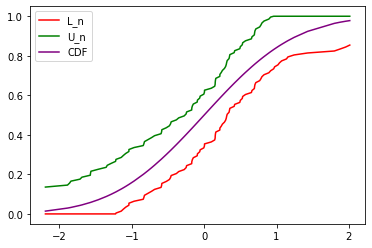
\includegraphics{Figure-08-01}
\end{figure}

    

\begin{python}
# 1000 iterations with Normal distribution
bounds = []
for k in tqdm(range(1000)):
    n = 100
    alpha = 0.05
    r = norm.rvs(size=n)
    epsilon = math.sqrt((1 / (2 * n)) * math.log(2 / alpha))
    F_n = lambda x : sum(r < x) / n
    L_n = lambda x : max(F_n(x) - epsilon, 0)
    U_n = lambda x : min(F_n(x) + epsilon, 1)
    # xx = sorted(r)
    xx = r # No need to sort without plotting
    
    df = pd.DataFrame({
        'x': xx, 
        'F_n': np.array(list(map(F_n, xx))), 
        'U_n': np.array(list(map(U_n, xx))), 
        'L_n': np.array(list(map(L_n, xx))), 
        'CDF': np.array(list(map(norm.cdf, xx)))
    })
    all_in_bounds = ((df['U_n'] >= df['CDF']) & (df['CDF'] >= df['L_n'])).all()
    bounds.append(all_in_bounds)
    
print('Average fraction in bounds: %.3f' % np.array(bounds).mean())
\end{python}
\begin{console}
100\%|███████████████████████████████████████████████████████████████████████████
████████████████████████████████████████████████████████████████████████████████
████████████████████████████████████████| 1000/1000 [01:05<00:00, 15.19it/s]
\end{console}
\begin{console}
Average fraction in bounds: 0.954
\end{console}

\begin{python}
# One iteration wtih Cauchy distribution
n = 100
alpha = 0.05
r = cauchy.rvs(size=n)
epsilon = math.sqrt((1 / (2 * n)) * math.log(2 / alpha))
F_n = lambda x : sum(r < x) / n
L_n = lambda x : max(F_n(x) - epsilon, 0)
U_n = lambda x : min(F_n(x) + epsilon, 1)
xx = sorted(r)
df = pd.DataFrame({
    'x': xx, 
    'F_n': np.array(list(map(F_n, xx))), 
    'U_n': np.array(list(map(U_n, xx))), 
    'L_n': np.array(list(map(L_n, xx))), 
    'CDF': np.array(list(map(norm.cdf, xx)))
})
df['in_bounds'] = (df['U_n'] >= df['CDF']) & (df['CDF'] >= df['L_n'])
plt.plot( 'x', 'L_n', data=df, color='red')
plt.plot( 'x', 'U_n', data=df, color='green')
plt.plot( 'x', 'CDF', data=df, color='purple')
plt.legend()
\end{python}

\begin{figure}[H]
\centering
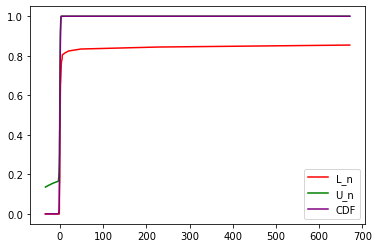
\includegraphics{Figure-08-02}
\end{figure}


\begin{python}
# 1000 iterations with Cauchy distribution
bounds = []
for k in tqdm(range(1000)):
    n = 100
    alpha = 0.05
    r = cauchy.rvs(size=n)
    epsilon = math.sqrt((1 / (2 * n)) * math.log(2 / alpha))
    F_n = lambda x : sum(r < x) / n
    L_n = lambda x : max(F_n(x) - epsilon, 0)
    U_n = lambda x : min(F_n(x) + epsilon, 1)
    # xx = sorted(r)
    xx = r # No need to sort without plotting
    df = pd.DataFrame({
        'x': xx, 
        'F_n': np.array(list(map(F_n, xx))), 
        'U_n': np.array(list(map(U_n, xx))), 
        'L_n': np.array(list(map(L_n, xx))), 
        'CDF': np.array(list(map(norm.cdf, xx)))
    })
    all_in_bounds = ((df['U_n'] >= df['CDF']) & (df['CDF'] >= df['L_n'])).all()
    bounds.append(all_in_bounds)
    
print('Average fraction in bounds: %.3f' % np.array(bounds).mean())
\end{python}
\begin{console}
100\%|███████████████████████████████████████████████████████████████████████████
████████████████████████████████████████████████████████████████████████████████
████████████████████████████████████████| 1000/1000 [01:04<00:00, 15.42it/s]
\end{console}
\begin{console}
Average fraction in bounds: 0.209
\end{console}

\textbf{Exercise 8.5.4}. Let \(X_{1}, \dots, X_{n} \sim F\) and let
\(\hat{F}_{n}(x)\) be the empirical distribution function. For a fixed
\(x\), use the central limit Theorem to find the limiting distribution
of \(\hat{F}_{n}(x)\).

\textbf{Solution}.
We have:
\[
\hat{F}_{n}(x) = \frac{\sum_{i=1}^{n} I\left(X_{i} \leq x \right)}{n}
\]
where
\begin{align*}I\left(X_{i} \leq x\right) =
    \begin{cases}
      1   & \text{if } X_{i} \leq x \\
      0   & \text{if } X_{i} > x
    \end{cases}       
\end{align*}
Let \(Y_{i} = I\left(X_{i} \leq x \right)\) for some fixed \(x\). From the
central limit Theorem,
\begin{align*}
\sqrt{n} (\bar{Y}_{n} - \mu_Y) & \leadsto N(0, \sigma_Y^{2}) \\
\bar{Y}_{n} & \leadsto N(\mu_Y, \sigma_Y^{2} / n)
\end{align*}
We can estimate the mean \(\mu_Y\) as
\[
\EXP(\hat{\mu}_{Y}) = \EXP(\bar{Y}_{n}) = n^{-1} \sum_{i=1}^{n} \EXP(I(X_{i} \leq x)) = n^{-1} \sum_{i=1}^{n} F(x) = \hat{F}_{n}(x).
\]
We can estimate the variance \(\sigma_Y^{2}\) as
\begin{align*}
\EXP(\hat{\sigma}_{Y}^{2}) 
  = \EXP(\VAR(\bar{Y}_{n})) 
& = n^{-1} \sum_{i=1}^{n} \EXP((Y_{i} - \bar{Y}_{n})^{2}) 
\\
& = n^{-1} \sum_{i=1}^{n} \left( \EXP(Y_{i}^{2}) - 2 \EXP(Y_{i} \bar{Y}_{n}) + \EXP(\bar{Y}_{n}^{2}) \right) 
\\
& \leq n^{-1} \sum_{i=1}^{n} \left( \EXP(Y_{i}) + \EXP(\bar{Y}_{n}^{2}) \right) \leq 2
\end{align*}
Therefore, for large \(n\), the limiting distribution has variance that
goes to 0 -- so \(\bar{Y}_{n} \leadsto \mu_Y\), or
\(I\left(X_{i} \leq x \right) \leadsto F(x)\) for every x. Then,
\(\hat{F}_{n}(x) \leadsto n^{-1} \sum_{i=1}^{n} F(x) = F(x)\),
and, as expected, \(F\) is the limiting distribution of \(F_n\).

\textbf{Exercise 8.5.5}. Let \(x\) and \(y\) be two distinct points.
Find \(\COV(\hat{F}_{n}(x), \hat{F}_{n}(y))\).

\textbf{Solution}.
We have:
\begin{align*}
\COV(\hat{F}_{n}(x), \hat{F}_{n}(y)) & = \EXP(\hat{F}_{n}(x) \hat{F}_{n}(y)) - \EXP(\hat{F}_{n}(x))\EXP(\hat{F}_{n}(y)) \\
&= \EXP(\hat{F}_{n}(x) \hat{F}_{n}(y)) - F(x)F(y)
\end{align*}
But:
\[
\hat{F}_{n}(x) \hat{F}_{n}(y) = \frac{1}{n^{2}} \sum_{i=1}^{n} \sum_{j=1}^{n} I(X_{i} \leq x) I(X_{j} \leq y)
\]
so
\begin{align*}
\EXP(\hat{F}_{n}(x) \hat{F}_{n}(y)) & = \frac{1}{n^{2}} \sum_{i=1}^{n} \sum_{j=1}^{n} \EXP(I(X_{i} \leq x) I(X_{j} \leq y)) \\
&= \frac{1}{n^{2}} \sum_{i=1}^{n} \sum_{j=1}^{n} \PROB(X_{i} \leq x, X_{j} \leq y) \\
&= \frac{1}{n^{2}} \sum_{i=1}^{n} \sum_{j=1}^{n} \PROB(X_{i} \leq x | X_{j} \leq y) \PROB(X_{j} \leq y) \\
&= \frac{1}{n^{2}} \left( \sum_{i=1}^{n} F(\min\{x, y\}) + \sum_{i=1}^{n} \sum_{j=1, j \neq i}^{n} F(x)F(y) \right) \\
&= \frac{1}{n} F(\min\{x, y\}) + \left( 1 - \frac{1}{n}\right) F(x)F(y)
\end{align*}
Therefore, assuming \(x \leq y\),
\begin{align*}
\COV(\hat{F}_{n}(x), \hat{F}_{n}(y)) & = \EXP(\hat{F}_{n}(x) \hat{F}_{n}(y)) - \EXP(\hat{F}_{n}(x))\EXP(\hat{F}_{n}(y)) \\
&= \EXP(\hat{F}_{n}(x) \hat{F}_{n}(y)) - F(x)F(y) \\
&= \frac{1}{n} F(\min\{x, y\}) + \left( 1 - \frac{1}{n}\right) F(x)F(y) - F(x)F(y) \\
&= \frac{F(x)(1 - F(y))}{n}
\end{align*}

\textbf{Exercise 8.5.6}. Let \(X_{1}, \dots, X_{n} \sim F\) and let
\(\hat{F}\) be the empirical distribution function. Let \(a < b\) be
fixed numbers and define \(\theta = T(F) = F(b) - F(a)\). Let
\(\hat{\theta} = T(\hat{F}_{n}) = \hat{F}_{n}(b) - \hat{F}_{n}(a)\).
\begin{itemize}[tightlist]
\item
  Find the estimated standard error of \(\hat{\theta}\).
\item
  Find an expression for an approximate \(1 - \alpha\) confidence
  interval for \(\theta\).
\end{itemize}

\textbf{Solution}.
\textbf{(a)}
The estimated mean for \(\hat{\theta}\) is
\(\EXP(\hat{\theta}) = \EXP(\hat{F}_{n}(b) - \hat{F}_{n}(a)) = \EXP(\hat{F}_{n}(b)) - \EXP(\hat{F}_{n}(a)) = F(b) - F(a) = \theta\).
The estimated variance for \(\hat{\theta}\) is
\[
\VAR(\hat{\theta}) = \EXP(\hat{\theta}^{2}) - \EXP(\hat{\theta})^{2}
\]
But
\begin{align*}
\EXP(\hat{\theta}^{2}) & = \EXP((\hat{F}_{n}(b) - \hat{F}_{n}(a))^{2})  \\
&= \EXP(\hat{F}_{n}(a)^{2} + \hat{F}_{n}(b)^{2} - 2 \hat{F}_{n}(a)\hat{F}_{n}(b)) \\
&= \EXP(\hat{F}_{n}(a)^{2}) + \EXP(\hat{F}_{n}(b)^{2}) - 2 \EXP(\hat{F}_{n}(a)\hat{F}_{n}(b))
\end{align*}
\begin{align*}
\EXP(\hat{F}_{n}(a)^{2}) & = \EXP\left(\left(\frac{1}{n} \sum_{i=1}^{n} I(X_{i} \leq a)\right)^{2}\right) \\
& = \frac{1}{n^{2}} \left(\sum_{i=1}^{n} \EXP \left( I(X_{i} \leq a)^{2} \right) + \sum_{i=1}^{n} \sum_{j=1, j \neq i}^{n} \EXP\left( I(X_{i} \leq a) I(X_{j} \leq a) \right) \right) \\
& = \frac{1}{n^{2}} \left(\sum_{i=1}^{n} \EXP \left( I(X_{i} \leq a) \right) + \sum_{i=1}^{n} \sum_{j=1, j \neq i}^{n} \EXP\left( I(X_{i} \leq a) I(X_{j} \leq a) \right) \right) \\
& = \frac{1}{n^{2}} \left(\sum_{i=1}^{n} \PROB \left( X_{i} \leq a \right) + \sum_{i=1}^{n} \sum_{j=1, j \neq i}^{n} \PROB\left( X_{i} \leq a, X_{j} \leq a \right) \right) \\
& = \frac{1}{n^{2}} \left(n F(a) + n(n-1) F(a)^{2} \right) \\
&= F(a) \frac{1}{n} + F(a)^{2} \left(1 - \frac{1}{n} \right) \\
\EXP(\hat{F}_{n}(b)^{2}) & = F(b) \frac{1}{n} + F(b)^{2} \left(1 - \frac{1}{n} \right)
\end{align*}
From the previous exercise,
\[
\EXP(\hat{F}_{n}(a)\hat{F}_{n}(b)) = \frac{1}{n} F(a) + \left( 1 - \frac{1}{n}\right) F(a)F(b)
\]
Putting it together,
\begin{align*}
\EXP(\hat{\theta}^{2}) 
&= \EXP(\hat{F}_{n}(a)^{2}) + \EXP(\hat{F}_{n}(b)^{2}) - 2 \EXP(\hat{F}_{n}(a)\hat{F}_{n}(b)) \\
&=   F(a) \frac{1}{n} + F(a)^{2} \left(1 - \frac{1}{n} \right) +  F(b) \frac{1}{n} + F(b)^{2} \left(1 - \frac{1}{n} \right) - 2 \left( \frac{1}{n} F(a) + \left( 1 - \frac{1}{n}\right) F(a)F(b) \right) \\
&=  \frac{1}{n} \left(F(b) - F(a)\right) + \left( 1 - \frac{1}{n}\right) \left( F(b) - F(a) \right)^{2} \\
&=  \frac{1}{n} \theta + \left( 1 - \frac{1}{n} \right) \theta^{2} \\
\VAR(\hat{\theta}) &=  \EXP(\hat{\theta}^{2}) - \EXP(\hat{\theta})^{2} \\
&=  \frac{1}{n} \theta + \left( 1 - \frac{1}{n} \right) \theta^{2} - \theta^{2} \\
&= \frac{\theta (1 - \theta)}{n} 
\end{align*}
Finally, the estimated standard error is
\[
\SE (\hat{\theta}) = \sqrt{\VAR(\hat{\theta})} = \sqrt{\frac{\hat{\theta}(1 - \hat{\theta})}{n}}
\]
\textbf{(b)}
An approximate \(1 - \alpha\) confidence interval is
\[
\hat{\theta} \pm z_{\alpha/2}\SE (\hat{\theta}) = \hat{\theta} \pm z_{\alpha/2} \sqrt{\frac{\hat{\theta}(1 - \hat{\theta})}{n}}
\]

\textbf{Exercise 8.5.7}. Data on the magnitudes of earthquakes near Fiji
are available on the course website.
\begin{itemize}[tightlist]
\item
  Estimate the CDF.
\item
  Compute and plot a 95\% confidence envelope for F.
\item
  Find an approximate 95\% confidence interval for F(4.9) - F(4.3).
\end{itemize}

\begin{python}
import pandas as pd
data = pd.read_csv('data/fijiquakes.csv', sep='\t')
r = np.array(data['mag'])
\end{python}

\begin{python}
n = len(r)
alpha = 0.05
epsilon = math.sqrt((1 / (2 * n)) * math.log(2 / alpha))
F_n = lambda x : sum(r < x) / n
L_n = lambda x : max(F_n(x) - epsilon, 0)
U_n = lambda x : min(F_n(x) + epsilon, 1)
xx = sorted(r)
df = pd.DataFrame({
    'x': xx, 
    'F_n': np.array(list(map(F_n, xx))), 
    'U_n': np.array(list(map(U_n, xx))), 
    'L_n': np.array(list(map(L_n, xx)))
})
plt.plot( 'x', 'L_n', data=df, color='red')
plt.plot( 'x', 'U_n', data=df, color='green')
plt.plot( 'x', 'F_n', data=df, color='blue')
plt.legend()
\end{python}

\begin{figure}[H]
\centering
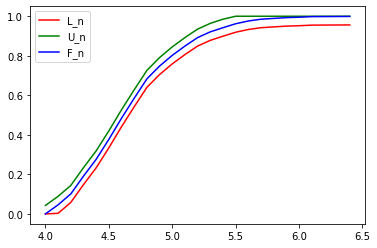
\includegraphics{Figure-08-03}
\end{figure}


\begin{python}
# Now to find the confidence interval, using the result from 8.5.6:
import math
from scipy.stats import norm
z_95 = norm.ppf(.975)
theta = F_n(4.9) - F_n(4.3)
se = math.sqrt(theta * (1 - theta) / n)
print('95%% confidence interval: (%.3f, %.3f)' % ((theta - z_95 * se), (theta + z_95 * se)))
\end{python}
\begin{console}
95\% confidence interval: (0.526, 0.588)
\end{console}

\textbf{Exercise 8.5.8}. Get the data on eruption times and waiting
times between eruptions of the old faithful geyser from the course
website.
\begin{itemize}[tightlist]
\item
  Estimate the mean waiting time and give a standard error for the
  estimate.
\item
  Also, give a 90\% confidence interval for the mean waiting time.
\item
  Now estimate the median waiting time.
\end{itemize}
In the next chapter we will see how to get the standard error for the
median.

\begin{python}
import numpy as np
import pandas as pd
data = pd.read_csv('data/geysers.csv', sep=',')
r = np.array(data['waiting'])
\end{python}

\begin{python}
# Estimate the mean waiting time and give a standard error for the estimate.
theta = r.mean()
se = np.std(r, ddof=1) / np.sqrt(len(r))
## Alternatively:
# from scipy.stats import sem
# se = sem(r)
print("Estimated mean: %.3f" % theta)
print("Estimated SE: %.3f" % se)
\end{python}
\begin{console}
Estimated mean: 70.897
Estimated SE: 0.824
\end{console}

\begin{python}
# Also, give a 90% confidence interval for the mean waiting time.
import math
from scipy.stats import norm
z_90 = norm.ppf(.95)
print('90%% confidence interval: (%.3f, %.3f)' % ((theta - z_90 * se), (theta + z_90 * se)))
\end{python}
\begin{console}
90\% confidence interval: (69.541, 72.253)
\end{console}

\begin{python}
# Now estimate the median time
median = np.median(r)
print("Estimated median time: %.3f" % median)
\end{python}
\begin{console}
Estimated median time: 76.000
\end{console}

\textbf{Exercise 8.5.9}. 100 people are given a standard antibiotic to
treat an infection and another 100 are given a new antibiotic. In the
first group, 90 people recover; in the second group, 85 people recover.
Let \(p_{1}\) be the probability of recovery under the standard treatment,
and let \(p_{2}\) be the probability of recovery under the new treatment.
We are interested in estimating \(\theta = p_{1} - p_{2}\). Provide an
estimate, standard error, an 80\% confidence interval and a 95\%
confidence interval for \(\theta\).

\textbf{Solution}. Let \(X_{1}, \dots, X_{1}00\) be indicator random
variables (0 or 1) determining recovery on the first group, and
\(Y_{1}, \dots, Y_{1}00\) indicating recovery on the second group. From the
problem formulation, we can assume \(X_{i} \sim \text{Bernoulli}(p_{1})\)
and \(Y_{i} \sim \text{Bernoulli}(p_{2})\). \(n_{1} = n_{2} = 100\), so we can
use \(n\) to refer to both.
If \(\theta = p_{1} - p_{2}\), then from exercise 8.5.2:
\[
\hat{\theta} = \hat{p}_{1} - \hat{p}_{2}
\]
\[
\SE (\hat{\theta}) = \sqrt{\frac{\hat{p}_{1}(1 - \hat{p}_{1})}{n} + \frac{\hat{p}_{2}(1 - \hat{p}_{2})}{n}}
\]

\begin{python}
import math
p_hat_1 = 0.9
p_hat_2 = 0.85
n = 100
theta_hat = p_hat_1 - p_hat_2
se_theta_hat = math.sqrt((p_hat_1 * (1 - p_hat_1) + p_hat_2 * (1 - p_hat_2)) / n)
print('Estimated mean: %.3f' % theta_hat)
print('Estimated SE: %.3f'   % se_theta_hat)
\end{python}
\begin{console}
Estimated mean: 0.050
Estimated SE: 0.047
\end{console}

\begin{python}
from scipy.stats import norm
z_80 = norm.ppf(.9)
z_95 = norm.ppf(.975)
print('80%% confidence interval: (%.3f, %.3f)' % ((theta_hat - z_80 * se_theta_hat), 
                                                 (theta_hat + z_80 * se_theta_hat)))
print('95%% confidence interval: (%.3f, %.3f)' % ((theta_hat - z_95 * se_theta_hat), 
                                                 (theta_hat + z_95 * se_theta_hat)))
\end{python}
\begin{console}
80\% confidence interval: (-0.010, 0.110)
95\% confidence interval: (-0.041, 0.141)
\end{console}

\textbf{Exercise 8.5.10}. In 1975, an experiment was conducted to see if
cloud seeding produced rainfall. 26 clouds were seeded with silver
nitrate and 26 were not. The decision to seed or not was made at random.
Get the data from the provided link.
Let \(\theta\) be the difference in the median precipitation from the
two groups.
\begin{itemize}[tightlist]
\item
  Estimate \(\theta\).
\item
  Estimate the standard error of the estimate and produce a 95\%
  confidence interval.
\end{itemize}

\begin{python}
import numpy as np
import pandas as pd
from tqdm import tqdm
data = pd.read_csv('data/cloud_seeding.csv', sep=',')
X = data['Seeded_Clouds']
Y = data['Unseeded_Clouds']
\end{python}

\begin{python}
theta_hat = X.median() - Y.median()
print('Estimated mean: %.3f' % theta_hat)
\end{python}
\begin{console}
Estimated mean: 177.400
\end{console}

\begin{python}
# Using bootstrap (from chapter 9):
nx = len(X)
ny = len(Y)
B = 10000
t_boot = np.zeros(B)
for i in tqdm(range(B)):
    xx = X.sample(n=nx, replace=True)
    yy = Y.sample(n=ny, replace=True)
    t_boot[i] = xx.median() - yy.median()
    
se = np.array(t_boot).std()
print('Estimated SE: %.3f' % se)
\end{python}
\begin{console}
100\%|███████████████████████████████████████████████████████████████████████████
████████████████████████████████████████████████████████████████████████████████
████████████████████████████████████| 10000/10000 [00:05<00:00, 1863.74it/s]
\end{console}
\begin{console}
Estimated SE: 63.420
\end{console}

\begin{python}
# See example 9.5, page 135
from scipy.stats import norm
z_95 = norm.ppf(.975)
normal_conf = (theta_hat - z_95 * se, theta_hat + z_95 * se)
percentile_conf = (np.quantile(t_boot, .025), np.quantile(t_boot, .975))
pivotal_conf = (2*theta_hat - np.quantile(t_boot, 0.975), 
                2*theta_hat - np.quantile(t_boot, .025))
print('95%% confidence interval (Normal): \t %.3f, %.3f' % normal_conf)
print('95%% confidence interval (percentile): \t %.3f, %.3f' % percentile_conf)
print('95%% confidence interval (pivotal): \t %.3f, %.3f' % pivotal_conf)
\end{python}
\begin{console}
95\% confidence interval (Normal):        53.099, 301.701
95\% confidence interval (percentile):    38.336, 266.201
95\% confidence interval (pivotal):       88.599, 316.464
\end{console}


% Chapter 9
\section*{9. The Bootstrap}\label{the-bootstrap}
Let \(X_{1}, \dots, X_{n} \sim F\) be random variables distributed according
to \(F\), and
\[
T_{n} = g(X_{1}, \dots, X_{n})
\]
be a \textbf{statistic}, that is, any function of the data. Suppose we
want to know \(\VAR_F(T_{n})\), the variance of \(T_{n}\).
For example, if \(T_{n} = n^{-1}\sum_{i=1}^{n}X_{i}\) then
\(\VAR_F(T_{n}) = \sigma^{2}/n\) where
\(\sigma^{2} = \int (x - \mu)^{d}F(x)\) and \(\mu = \int x dF(x)\).

\subsection*{9.1 Simulation}\label{bootstrap:simulation}
Suppose we draw iid samples \(Y_{1}, \dots, Y_B \sim G\). By the law of
large numbers,
\[
\bar{Y}_{n} = \frac{1}{B} \sum_{j=1}^B Y_{j} \; \xrightarrow{\textrm{P}} \int y dG(y) = \EXP(Y)
\]
as \(B \rightarrow \infty\). So if we draw a large sample from \(G\), we
can use the sample mean to approximate the mean of the distribution.
More generally, if \(h\) is any function with finite mean then, as
\(B \rightarrow \infty\),
\[
\frac{1}{B} \sum_{j=1}^B h(Y_{j}) \; \xrightarrow{\textrm{P}} \int h(y) dG(y) = \EXP(h(Y))
\]
In particular, for functions \(a(Y_{j}) = Y_{j}^{2}\) and \(b(Y_{j}) = Y_{j}\),
\[
\frac{1}{B} \sum_{j=1}^B (Y_{j} - \bar{Y}) 
= \frac{1}{B} \sum_{j=1}^B Y_{j}^{2} - \left(\frac{1}{B} \sum_{j=1}^B Y_{j} \right)^{2}
\xrightarrow{\textrm{P}} \int y^{2} dG(y) - \left( \int y dG(y) \right)^{2} = \VAR(Y)
\]
So we can use the sample variance of the simulated values to approximate
\(\VAR(Y)\).

\subsection*{9.2 Bootstrap Variance
Estimation}\label{bootstrap:variance}
To simulate from the distribution of a statistic \(T_{n}\) when the data
is assumed to have distribution \(\hat{F}_{n}\), we simulate
\(X_{1}^{*}, \dots, X_{n}^{*}\) from \(\hat{F}_{n}\) and then compute the
statistic over these values, \(T_{n}^{*} = g(X_{1}^{*}, \dots, X_{n}^{*})\).
\begin{align*}
\text{Real world} \quad      & F         & \Longrightarrow\quad & X_{1}, \dots, X_{n}        & \Longrightarrow & \quad T_{n} = g(X_{1}, \dots, X_{n}) \\
\text{Bootstrap world} \quad & \hat{F}_{n} & \Longrightarrow\quad  & X_{1}^{*}, \dots, X_{n}^{*} & \Longrightarrow & \quad T_{n}^{*} = g(X_{1}^{*}, \dots, X_{n}^{*})
\end{align*}
\textbf{Drawing an observation from \(\hat{F}_{n}\) is equivalent to
drawing one point at random from the original data set.}
\paragraph{Bootstrap Variance
Estimation}\label{bootstrap:variance}
\begin{enumerate}[tightlist,label={\arabic*.}]
\item
  Draw \(X_{1}^{*}, \dots, X_{n}^{*} \sim \hat{F}_{n}\).
\item
  Compute \(T_{n}^{*} = g(X_{1}^{*}, \dots, X_{n}^{*})\).
\item
  Repeat steps 1 and 2, \(B\) times, to get
  \(T_{n, 1}^{*}, \dots, T_{n, B}^{*}\).
\item
  Let
\end{enumerate}
\[
v_{\text{boot}} = \frac{1}{B} \sum_{b=1}^B \left( T_{n, b}^{*} - \frac{1}{B} \sum_{r=1}^B T_{n, r}^{*} \right)^{2}
\]

\subsection*{9.3 Bootstrap Confidence
Intervals}\label{bootstrap-confidence-intervals}
\textbf{Normal Interval}.
\[
T_{n} \pm z_{\alpha/2} \widehat{\SE}_\text{boot}
\]
where \(\widehat{\SE}_\text{boot}\) is the bootstrap estimate of the
standard error. This is not accurate unless the distribution of \(T_{n}\)
is close to Normal.
\textbf{Pivotal Intervals}.
Let \(\theta = T(F)\), \(\hat{\theta}_{n} = T(\hat{F}_{n})\) and define the
\textbf{pivot} \(R_{n} = \hat{\theta}_{n}  - \theta\). Let
\(\hat{\theta}_{n, 1}^{*}, \dots, \hat{\theta}_{n, B}^{*}\) define bootstrap
replications of \(\hat{\theta}_{n}\). Let \(H(r)\) denote the CDF of the
pivot:
\[
H(r) = \PROB_F(R_{n} \leq r)
\]
Define the interval \(C_{n}^{*} = (a, b)\) where
\[
a = \hat{\theta}_{n} - H^{-1}\left( 1 - \frac{\alpha}{2} \right) 
\quad\text{and}\quad
b = \hat{\theta}_{n} - H^{-1}\left( \frac{\alpha}{2} \right) 
\]
Then,
\begin{align*}
\PROB(a \leq \theta \leq b) &= \PROB(a - \hat{\theta}_{n} \leq \theta - \hat{\theta}_{n} \leq b - \hat{\theta}_{n}) \\
&= \PROB(\hat{\theta}_{n} - b \leq \hat{\theta}_{n} - \theta \leq \hat{\theta}_{n} - a) \\
&= \PROB(\hat{\theta}_{n} - b \leq R_{n} \leq \hat{\theta}_{n} - a) \\
&= H(\hat{\theta}_{n} - a) - H(\hat{\theta}_{n} - b) \\
&= H\left(H^{-1}\left( 1 - \frac{\alpha}{2} \right) \right) - H\left(H^{-1}\left( \frac{\alpha}{2} \right)\right) \\
&= 1 - \frac{\alpha}{2}  - \frac{\alpha}{2} = 1 - \alpha
\end{align*}
Hence \(C_{n}^{*}\) is an exact \(1 - \alpha\) confidence interval for
\(\theta\).
Unfortunately, \(a\) and \(b\) depend on the unknown distribution \(H\),
but we can form a bootstrap estimate for it:
\[
\hat{H}(r) = \frac{1}{B} \sum_{b=1}^B I(R_{n, b}^{*} \leq r)
\]
where \(R_{n, b}^{*} = \hat{\theta}_{n, b}^{*} - \hat{\theta}_{n}\).
Let \(r_\beta^{*}\) denote the \(\beta\) sample quantile of
\((R_{n, 1}^{*}, \dots, R_{n, B}^{*})\), and let \(\theta_\beta^{*}\) denote
the \(\beta\) sample quantile of
\((\theta_{n, 1}^{*}, \dots, \theta_{n, B}^{*})\). Note that
\(r_\beta^{*} = \theta_\beta^{*} - \hat{\theta}_{n}\). It follows an
approximate \(1 - \alpha\) confidence interval
\(C_{n} = (\hat{a}, \hat{b})\) where
\begin{align*}
\hat{a} 
&= \hat{\theta}_{n} - \hat{H}^{-1}\left(1 - \frac{\alpha}{2}\right) 
&= \hat{\theta}_{n} - r_{1 - \alpha/2}^{*} 
&= 2\hat{\theta}_{n} - \theta_{1 - \alpha/2}^{*} \\
\hat{b} 
&= \hat{\theta}_{n} - \hat{H}^{-1}\left(\frac{\alpha}{2}\right) 
&= \hat{\theta}_{n} - r_{\alpha/2}^{*} 
&= 2\hat{\theta}_{n} - \theta_{\alpha/2}^{*} 
\end{align*}
The \textbf{\(1 - \alpha\) bootstrap pivotal confidence} is
\[
C_{n} = \left(2 \hat{\theta}_{n} - \hat{\theta}_{1 - \alpha/2}^{*}, \; 2 \hat{\theta}_{n} - \hat{\theta}_{\alpha/2}^{*} \right)
\]

\textbf{Theorem 9.3}. Under weak conditions on \(T(F)\),
\[
\lim _{n \rightarrow \infty} \PROB_F\left(T(F) \in C_{n}\right) \rightarrow 1 - \alpha
\]
\textbf{Percentile Intervals}.
The \textbf{bootstrap percentile interval} is defined by
\[
C_{n} = \left( \theta_{\alpha/2}^{*}, \; \theta_{1 - \alpha/2}^{*}\right)
\]

\subsection*{9.5 Technical Appendix}
\paragraph{The Jacknife}\label{the-jacknife}
This method is less computationally expensive than bootstraping, but it
is less general -- it does \emph{not} produce consistent estimates of
the standard errors of the sample quantiles.
Let \(T_{n} = T(X_{1}, \dots, X_{n})\) be a statistic and let \(T_{(-i)}\)
denote the statistic with the \(i\)-th observation removed. Let
\(\bar{T}_{n} = n^{-1} \sum_{i=1}^{n} T_{(-1)}\). The jacknife estimate
of \(\VAR(T_{n})\) is
\[
v_\text{jack} = \frac{n - 1}{n} \sum_{i=1}^{n} \left(T_{(-i)} - \bar{T}_{n} \right)^{2}
\]
and the jacknife estimate of the standard error is
\(\widehat{\SE}_\text{jack} = \sqrt{v_\text{jack}}\).
Under suitable conditions on \(T\) it can be shown that
\(v_\text{jack} / \VAR(T_{n}) \xrightarrow{\textrm{P}} 1\).
\paragraph{Justification for the Percentile
Interval}\label{justification-for-the-percentile-interval}
Suppose there exists a monotone transformation \(U = m(T)\) such that
\(U \sim N(\phi, c^{2})\) where \(\phi = m(\theta)\).
Let \(U_t^{*} = m(\theta_{n, b}^{*})\). Let \(u_\beta^{*}\) be the sample
quantile of the \(U_b^{*}\)s. Since a monotone transformation preserves
quantiles, we have that \(u_{\alpha/2}^{*} = m(\theta_{\alpha/2}^{*})\).
Also, since \(U \sim N(\phi, c^{2})\) the \(\alpha/2\) quantile of \(U\)
is \(\phi - z_{\alpha/2}c\). Hence
\(u_{\alpha/2}^{*} = \phi - z_{\alpha/2}c\). Similarly,
\(u_{1 - \alpha/2}^{*} = \phi + z_{\alpha/2}c\).
Therefore,
\begin{align*}
\PROB(\theta_{\alpha/2}^{*} \leq \theta \leq \theta_{1 - \alpha/2}^{*}) &=
\PROB(m(\theta_{\alpha/2}^{*}) \leq m(\theta) \leq m(\theta_{1 - \alpha/2}^{*})) \\
&= \PROB(u_{\alpha/2}^{*} \leq \phi \leq u_{1 - \alpha/2}^{*}) \\
&= \PROB(U - cz_{\alpha/2} \leq \phi \leq U + cz_{1 - \alpha/2}) \\
&= \PROB\left(-z_{\alpha/2} \leq \frac{Y - \phi}{c} \leq z_{1 - \alpha/2} \right) \\
&= 1 - \alpha
\end{align*}

\subsection*{9.6 Exercises}

\textbf{Exercise 9.6.1}. Consider the data in example 9.6.
\begin{itemize}[tightlist]
\item
  Find the plug-in estimate of the correlation coefficient.\\
\item
  Estimate the standard error using the bootstrap.\\
\item
  Find a 95\% confidence interval using all three methods.
\end{itemize}

\begin{python}
# Data from example 9.6:
LSAT = [576, 635, 558, 578, 666, 580, 555, 661, 651, 605, 653, 575, 545, 572, 594]
GPA = [3.39, 3.30, 2.81, 3.03, 3.44, 3.07, 3, 3.43, 3.36, 3.13, 3.12, 2.74, 2.76, 2.88, 3.96]
\end{python}

\begin{python}
import math
import numpy as np
import pandas as pd
from tqdm import tqdm_notebook
df = pd.DataFrame({'LSAT': LSAT, 'GPA': GPA})
df.plot.scatter(x='LSAT', y='GPA')
\end{python}

\begin{figure}[H]
\centering
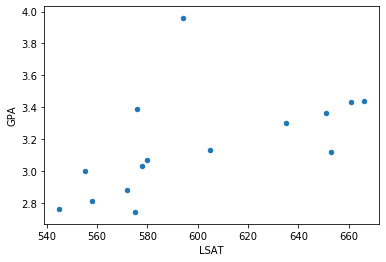
\includegraphics{Figure-09-01}
\end{figure}


\begin{python}
# Plug-in estimates for mean and correlation
X = df['LSAT'].to_numpy()
Y = df['GPA'].to_numpy()
def corr(X, Y):
    mu_x = X.mean()
    mu_y = Y.mean()
    return sum((X - mu_x) * (Y - mu_y)) / math.sqrt(sum((X - mu_x)**2) * sum((Y - mu_y)**2))
  
theta_hat = corr(X, Y)
    
print('Estimated correlation coefficient: %.4f' % corr(X, Y))
\end{python}
\begin{console}
Estimated correlation coefficient: 0.5459
\end{console}

\begin{python}
# Bootstrap for SE of correlation coefficient
nx = len(X)
ny = len(Y)
B = 1000000
t_boot = np.empty(B)
for i in tqdm_notebook(range(B)):
    xx = np.random.choice(X, nx, replace=True)
    yy = np.random.choice(Y, ny, replace=True)
    t_boot[i] = corr(xx, yy)
    
se = t_boot.std()
print('Estimated SE of correlation coefficient: %.4f' % se)
\end{python}
\begin{console}
Estimated SE of correlation coefficient: 0.2674
\end{console}

\begin{python}
# Confidence intervals obtained from bootstrap
from scipy.stats import norm
z = norm.ppf(.975)
normal_conf = (theta_hat - z * se, theta_hat + z * se)
percentile_conf = (np.quantile(t_boot, .025), np.quantile(t_boot, .975))
pivotal_conf = (2*theta_hat - np.quantile(t_boot, 0.975), 
                2*theta_hat - np.quantile(t_boot, .025))
print('95%% confidence interval (Normal): \t %.3f, %.3f' % normal_conf)
print('95%% confidence interval (percentile): \t %.3f, %.3f' % percentile_conf)
print('95%% confidence interval (pivotal): \t %.3f, %.3f' % pivotal_conf)
\end{python}
\begin{console}
95\% confidence interval (Normal):        0.022, 1.070
95\% confidence interval (percentile):    -0.503, 0.522
95\% confidence interval (pivotal):       0.569, 1.594
\end{console}

\textbf{Exercise 9.6.2}. (Computer Experiment). Conduct a simulation to
compare the four bootstrap confidence interval methods.
Let \(n = 50\) and let \(T(F) = \int (x - \mu)^{3} dF(x) / \sigma^{3}\) be
the skewness. Draw \(Y_{1}, \dots, Y_{n} \sim N(0, 1)\) and set
\(X_{i} = e^{Y_{i}}\), \(i = 1, \dots, n\). Construct the four types of
bootstrap 95\% intervals for \(T(F)\) from the data \(X_{1}, \dots, X_{n}\).
Repeat this whole thing many times and estimate the true coverage of the
four intervals.

\begin{python}
import numpy as np
from tqdm import tqdm_notebook
from scipy.stats import norm
def create_data(n=50):
    y = norm.rvs(size=n)
    return np.exp(y)
def skewness(x):
    n = len(x)
    mu = sum(x) / n
    var = sum((x - mu)**2) / n
    return sum((x - mu)**3 / (n * var**(3/2)))
def bootstrap_values(x, B=10000, show_progress=True):
    n = len(x)
    t_boot = np.empty(B)
    iterable = tqdm_notebook(range(B)) if show_progress else range(B)
    for i in iterable:
        xx = np.random.choice(x, n, replace=True)
        t_boot[i] = skewness(xx)
    return t_boot
def bootstrap_intervals(theta_hat, t_boot, alpha=0.05):
    se = t_boot.std()
    
    z = norm.ppf(1 - alpha/2)
    q_half_alpha = np.quantile(t_boot, alpha/2)
    q_c_half_alpha = np.quantile(t_boot, 1 - alpha/2)
    normal_conf = (theta_hat - z * se, theta_hat + z * se)
    percentile_conf = (q_half_alpha, q_c_half_alpha)
    pivotal_conf = (2*theta_hat - q_c_half_alpha, 2*theta_hat - q_half_alpha)
    
    return normal_conf, percentile_conf, pivotal_conf
\end{python}

\begin{python}
# Creating the data
x = create_data(n=50)
# Nonparametric Bootstrap
theta_hat = skewness(x)
t_boot = bootstrap_values(x, B=100000)
normal_conf, percentile_conf, pivotal_conf = bootstrap_intervals(theta_hat, t_boot, alpha=0.05)
print('95%% confidence interval (Normal): \t %.3f, %.3f' % normal_conf)
print('95%% confidence interval (percentile): \t %.3f, %.3f' % percentile_conf)
print('95%% confidence interval (pivotal): \t %.3f, %.3f' % pivotal_conf)
\end{python}
\begin{console}
95\% confidence interval (Normal):        1.032, 2.638
95\% confidence interval (percentile):    1.154, 2.757
95\% confidence interval (pivotal):       0.912, 2.515
\end{console}
\textbf{Note}: parametric bootstrap is only covered in chapter 10. The
below assumes that ``four types of bootstrap'' in the exercise refers to
the 3 types of nonparametric bootstrap covered in chapter 9, plus
parametric bootstrap from chapter 10.
For the parametric bootstrap, assume \(X = e^Y\) where
\(Y \sim N(\mu, \sigma^{2})\). Then
\begin{align*}
\EXP(X) & = \EXP(e^Y) = \int_{-\infty}^{\infty} e^y \frac{1}{\sigma \sqrt{2 \pi}} e^{-\frac{1}{2} \left(\frac{y - \mu}{\sigma} \right)^{2}} dy = \frac{1}{\sigma \sqrt{2 \pi}} \int e^{y - \frac{1}{2}\left(\frac{y - \mu}{\sigma}\right)^{2}} dy = e^{\mu + \sigma^{2}/2} \\
\EXP(X^{2}) &= \EXP(e^{2Y}) = e^{2\mu + (2\sigma)^{2}/2} = e^{2\mu + 2\sigma^{2}}
\end{align*}
Solving the two equations for the moments we get parameter estimates:
\begin{align*}
\hat{\mu}_Y & = 4 \log \EXP(X) - \log \EXP(X^{2}) \\
\hat{\sigma}_Y & = \sqrt{\log \EXP(X^{2}) - 2 \log \EXP(X)}
\end{align*}
From these parameter estimates, we can generate bootstrap samples:
sample values for \(Y_{i} ~ N(\hat{\mu}_Y, \hat{\sigma}_Y^{2})\), calculate
\(X_{i} = Y_{i}\), and calculate the statistic \(T(X_{i})\) on each sample
generated this way.

\begin{python}
# Parametric bootstrap
# Assume X = e^Y, Y ~ N(\mu, \sigma^{2})
def estimate_parameters(x):
    log_e_x = np.log(x.mean())
    log_e_x2 = np.log((x**2).mean())
    
    mu_Y_hat = 4 * log_e_x - log_e_x2
    sigma_Y_hat = np.sqrt(log_e_x2 - 2 * log_e_x)
    
    return mu_Y_hat, sigma_Y_hat
def bootstrap_skewness_parametric(mu, sigma, n, B = 10000, show_progress=True):
    t_boot = np.empty(B)
    iterable = tqdm_notebook(range(B)) if show_progress else range(B)
    for i in iterable:
        xx = np.exp(norm.rvs(size=n, loc=n, scale=sigma))
        t_boot[i] = skewness(xx)
        
    return t_boot
def bootstrap_parametric_intervals(mu, t_boot, alpha=0.05):
    se = t_boot.std()
    z = norm.ppf(1 - alpha/2)
    
    return (theta_hat - z * se, theta_hat + z * se)
\end{python}

\begin{python}
mu_X_hat = x.mean()
mu_Y_hat, sigma_Y_hat = estimate_parameters(x)
t_boot = bootstrap_skewness_parametric(mu_Y_hat, sigma_Y_hat, 50, B=100000)
parametric_normal_conf = bootstrap_parametric_intervals(mu_X_hat, t_boot, alpha=0.05)
print('95%% confidence interval (Parametric Normal): \t %.3f, %.3f' % parametric_normal_conf)
\end{python}
\begin{console}
95\% confidence interval (Parametric Normal):     -0.181, 3.851
\end{console}

\begin{python}
# Repeat nonparametric bootstrap many times
n_experiments = 10
normal_conf = np.empty((n_experiments, 2))
percentile_conf = np.empty((n_experiments, 2))
pivotal_conf = np.empty((n_experiments, 2))
for i in tqdm_notebook(range(n_experiments)):
    theta_hat = skewness(x)
    t_boot_experiment = bootstrap_values(x, B=100000, show_progress=False)
    normal_conf[i], percentile_conf[i], 
                    pivotal_conf[i] = bootstrap_intervals(theta_hat, 
                                                          t_boot_experiment, 
                                                          alpha=0.05)
\end{python}

\begin{python}
print('Normal confidence lower bound: \t\t mean %.3f, SE %.3f' % 
      (normal_conf[:, 0].mean(), normal_conf[:, 0].std()))
print('Normal confidence upper bound: \t\t mean %.3f, SE %.3f' % 
      (normal_conf[:, 1].mean(), normal_conf[:, 1].std()))
print('Percentile confidence lower bound: \t mean %.3f, SE %.3f' % 
      (percentile_conf[:, 0].mean(), percentile_conf[:, 0].std()))
print('Percentile confidence upper bound: \t mean %.3f, SE %.3f' % 
      (percentile_conf[:, 1].mean(), percentile_conf[:, 1].std()))
print('Pivotal confidence lower bound: \t mean %.3f, SE %.3f' % 
      (pivotal_conf[:, 0].mean(), pivotal_conf[:, 0].std()))
print('Pivotal confidence upper bound: \t mean %.3f, SE %.3f' % 
      (pivotal_conf[:, 1].mean(), pivotal_conf[:, 1].std()))
\end{python}
\begin{console}
Normal confidence lower bound:           mean 1.031, SE 0.001
Normal confidence upper bound:           mean 2.639, SE 0.001
Percentile confidence lower bound:       mean 1.154, SE 0.002
Percentile confidence upper bound:       mean 2.762, SE 0.005
Pivotal confidence lower bound:          mean 0.907, SE 0.005
Pivotal confidence upper bound:          mean 2.515, SE 0.002
\end{console}

\begin{python}
# Repeat parametric bootstrap many times
n_experiments = 10
parametric_normal_conf = np.empty((n_experiments, 2))
for i in tqdm_notebook(range(n_experiments)):
    mu_X_hat = x.mean()
    mu_Y_hat, sigma_Y_hat = estimate_parameters(x)
    t_boot = bootstrap_skewness_parametric(mu_Y_hat, sigma_Y_hat, 50, B=100000, 
                                                                      show_progress=False)
    parametric_normal_conf[i] = bootstrap_parametric_intervals(mu_X_hat, t_boot, alpha=0.05)
\end{python}

\begin{python}
print('Parametric Normal confidence lower bound: \t mean %.3f, SE %.3f' % 
      (parametric_normal_conf[:, 0].mean(), parametric_normal_conf[:, 0].std()))
print('Parametric Normal confidence upper bound: \t mean %.3f, SE %.3f' % 
      (parametric_normal_conf[:, 1].mean(), parametric_normal_conf[:, 1].std()))
\end{python}
\begin{console}
Parametric Normal confidence lower bound:        mean -0.185, SE 0.003
Parametric Normal confidence upper bound:        mean 3.854, SE 0.003
\end{console}

\textbf{Exercise 9.6.3}. Let \(X_{1}, \dots, X_{n} \sim t_{3}\) where
\(n = 25\). Let \(\theta = T(F) = (q_{.75} - q_{.25})/1.34\) where
\(q_p\) denotes the \(p\)-th quantile. Do a simulation to compare the
coverage and length of the following confidence intervals for
\(\theta\):
\begin{itemize}[tightlist]
\item
  Normal interval with standard error from the bootstrap
\item
  Bootstrap percentile interval
\end{itemize}
Remark: the jacknife does not give a consistent estimator of the
variance of a quantile.

\textbf{Solution}. We will assume that \(t_{3}\) represents a
t-distribution with shape parameter 3.

\begin{python}
import numpy as np
from scipy.stats import t
from tqdm import tqdm_notebook
n = 25
X = t.rvs(3, size=25)
\end{python}

\begin{python}
def T(x):
    return (np.quantile(x, 0.75) - np.quantile(x, 0.25)) / 1.34
\end{python}

\begin{python}
theta_hat = T(X)
\end{python}

\begin{python}
# Run bootstrap
B = 1000000
t_boot = np.empty(B)
for i in tqdm_notebook(range(B)):
    xx = np.random.choice(X, n, replace=True)
    t_boot[i] = T(xx)
    
se_boot = t_boot.std()
alpha = 0.05
z = norm.ppf(1 - alpha/2)
q_half_alpha = np.quantile(t_boot, alpha/2)
q_c_half_alpha = np.quantile(t_boot, 1 - alpha/2)
normal_conf = (theta_hat - z * se_boot, theta_hat + z * se_boot)
percentile_conf = (q_half_alpha, q_c_half_alpha)
print('95%% confidence interval (Normal): \t %.3f, %.3f' % normal_conf)
print('95%% confidence interval (percentile): \t %.3f, %.3f' % percentile_conf)
\end{python}
\begin{console}
95\% confidence interval (Normal):        0.032, 2.089
95\% confidence interval (percentile):    0.605, 2.378
\end{console}

\textbf{Exercise 9.6.4}. Let \(X_{1}, \dots, X_{n}\) be distinct
observations (no ties). Show that there are
\[
\binom{2n - 1}{n}
\]
distinct bootstrap samples.
Hint: Imagine putting \(n\) balls into \(n\) buckets.

\textbf{Solution}.
Each bootstrap sample (random draws with replacement) will select
\(a_{i}\) copies of \(X_{i}\), where \(0 \leq a_{i} \leq n\) and
\(\sum_{i=1}^{n} a_{i} = n\), for integer \(a_{i}\). Each bootstrap sample is
uniquely represented by this sequence of variables, and each sequence of
variables uniquely determines a bootstrap sample -- so the number of
distinct bootstrap samples is equal to the number of solutions to this
equation, that is, the number of partitions of \(n\) into \(n\) buckets.
Lets write \(a_{i}\) explicitly in base 1, representing it as \(a_{i}\)
consecutive copies of the digit 1:
\begin{align*}
0_{10} & = \text{empty string}_{1} \\
1_{10} & = 1_{1} \\
2_{10} & = 11_{1} \\
3_{10} & = 111_{1} \\
4_{10} & = 1111_{1} \\
\vdots
\end{align*}
So a solution for
\[
a_{1} + a_{2} + \dots + a_{n} = n
\]
is uniquely represented by a sequence of \(2n - 1\) symbols, being \(n\)
digits \(1\) and \(n - 1\) plus signs. For example, if \(a_{1} = 3\),
\(a_{2} = 0\), \(a_{3} = 1\), then we write
\[
111 + + 1 + \dots = n
\]
The number of such solutions is then obtained by choosing \(n\) of the
\(2n - 1\) symbols to be digit \(1\) -- that is, \(\binom{2n - 1}{n}\).

\textbf{Exercise 9.6.5}. Let \(X_{1}, \dots, X_{n}\) be distinct
observations (no ties). Let \(X_{1}^{*}, \dots, X_{n}^{*}\) denote a bootstrap
sample and let \(\bar{X}_{n}^{*} = n^{-1}\sum_{i=1}^{n}X_{i}^{*}\). Find:
\begin{itemize}[tightlist]
\item
  \(\EXP(\bar{X}_{n}^{*} | X_{1}, \dots, X_{n})\)
\item
  \(\VAR(\bar{X}_{n}^{*} | X_{1}, \dots, X_{n})\)
\item
  \(\EXP(\bar{X}_{n}^{*})\)
\item
  \(\VAR(\bar{X}_{n}^{*})\)
\end{itemize}

\textbf{Solution}.
\textbf{(a)} \begin{align*}
\EXP(\bar{X}_{n}^{*} | X_{1}, \dots, X_{n}) &= \EXP\left(n^{-1}\sum_{i=1}^{n}X_{i}\right) = n^{-1}\sum_{i=1}^{n} \EXP(X_{i}) = \EXP(X)
\end{align*}
\textbf{(b)} \begin{align*}
\VAR(\bar{X}_{n}^{*} | X_{1}, \dots, X_{n}) & =
\EXP((\bar{X}_{n}^{*})^{2} | X_{1}, \dots, X_{n}) - \EXP(\bar{X}_{n}^{*} | X_{1}, \dots, X_{n})^{2} \\
&= \EXP\left(\left(n^{-1}\sum_{i=1}^{n}X_{i}\right)^{2}\right) - \EXP\left(n^{-1}\sum_{i=1}^{n}X_{i}\right)^{2} \\
&= n^{-2} \EXP\left(\sum_{i=1}^{n}X_{i}^{2} + \sum_{i=1}^{n} \sum_{j=1, j \neq i}^{n} X_{i} X_{j}\right) - \EXP(X)^{2} \\
&= n^{-2} \sum_{i=1}^{n} \EXP(X_{i}^{2}) + n^{-2} \sum_{i=1}^{n} \sum_{j=1, j \neq i}^{n} \EXP(X_{i} X_{j}) - \EXP(X)^{2}  \\
&= n^{-1} (\VAR(X) + \EXP(X)^{2}) + n^{-2} \sum_{i=1}^{n} \sum_{j=1, j \neq i}^{n} \EXP(X_{i}) \EXP(X_{j}) - \EXP(X)^{2} \\
&= n^{-1} (\VAR(X) + \EXP(X)^{2}) + n^{-1} (n - 1) \EXP(X)^{2} - \EXP(X)^{2} \\
&= \frac{1}{n}\VAR(X)
\end{align*}
\textbf{(c)} \begin{align*}
\EXP(\bar{X}_{n}^{*}) &= \EXP\left(n^{-1} \sum_{i=1}^{n}X_{i}^{*}\right) = n^{-1} \sum_{i=1}^{n} \EXP(X_{i}^{*}) = \EXP(X)
\end{align*}
\textbf{(d)} \begin{align*}
\VAR(\bar{X}_{n}^{*}) &= \EXP((\bar{X}_{n}^{*})^{2}) - \EXP(\bar{X}_{n}^{*})^{2} \\
&= \EXP\left(\left(n^{-1} \sum_{i=1}^{n}X_{i}^{*}\right)^{2}\right) - \EXP(X)^{2} \\
&= n^{-2} \sum_{i=1}^{n}\sum_{j=1}^{n} \EXP(X_{i}^{*} X_{j}^{*}) - \EXP(X)^{2}
\end{align*}
Now, the same value \(X_{k}\) may have been sampled twice in
\(\EXP(X_{i}^{*} X_{j}^{*})\). This always happens when \(i = j\), and
this happens with probability \(1 / n\) when \(i \neq j\). Thus,
\begin{align*}
\VAR(\bar{X}_{n}^{*}) 
&= n^{-2} \left(\sum_{i=1}^{n} \EXP(X_{i}^{2}) + \sum_{i=1}^{n} \sum_{j=1, j \neq i}^{n} \left( \frac{1}{n} \EXP(X_{i}^{2}) + \left(1 - \frac{1}{n}\right)\EXP(X_{i})\EXP(X_{j})\right) \right) - \EXP(X)^{2} \\
&= n^{-1} \EXP(X^{2}) + n^{-2} (n-1) \EXP(X^{2}) + n^{-2}(n-1)^{2} E(X)^{2} - \EXP(X)^{2} \\
&= n^{-2} (2n - 1) \left( \EXP(X^{2}) - \EXP(X)^{2} \right) \\
&= \frac{2n - 1}{n^{2}} \VAR(X)
\end{align*}

\textbf{Exercise 9.6.6}. (Computer Experiment). Let
\(X_{1}, \dots, X_{n} \sim N(\mu, 1)\). Let \(\theta = e^\mu\)and let
\(\hat{\theta} = e^{\bar{X}}\) be the mle. Create a dataset (using
\(\mu = 5\)) consisting of \(n = 100\) observations.
\textbf{(a)} Use the bootstrap to get the \(\SE \) and 95\%
confidence interval for \(\theta\).
\textbf{(b)} Plot a histogram of the bootstrap replications for the
parametric and non-parametric bootstraps. These are estimates of the
distribution of \(\hat{\theta}\). Compare this to the true sampling
distribution of \(\hat{\theta}\).

\begin{python}
import numpy as np
import pandas as pd
from scipy.stats import norm
from tqdm import tqdm_notebook
X = norm.rvs(loc=5, scale=1, size=100)
\end{python}

\begin{python}
# Get estimated value
theta_hat = np.exp(X.mean())
# Run nonparametric bootstrap
B = 1000000
t_boot_nonparam = np.empty(B)
n = len(X)
for i in tqdm_notebook(range(B)):
    xx = np.random.choice(X, n, replace=True)
    t_boot_nonparam[i] = np.exp(xx.mean())
    
se_boot = t_boot_nonparam.std()
alpha = 0.05
z = norm.ppf(1 - alpha/2)
normal_conf = (theta_hat - z * se_boot, theta_hat + z * se_boot)
print('95%% confidence interval (Normal): \t %.3f, %.3f' % normal_conf)
\end{python}
\begin{console}
95\% confidence interval (Normal):        104.486, 160.228
\end{console}

\begin{python}
# Run parametric bootstrap
mu_hat = X.mean()
theta_hat = np.exp(mu_hat)
B = 1000000
t_boot_param = np.empty(B)
n = len(X)
for i in tqdm_notebook(range(B)):
    xx = norm.rvs(size=n, loc=mu_hat, scale=1)
    t_boot_param[i] = np.exp(xx.mean())
    
se_boot_param = t_boot_param.std()
alpha = 0.05
z = norm.ppf(1 - alpha/2)
normal_conf_param = (theta_hat - z * se_boot_param, theta_hat + z * se_boot_param)
print('95%% confidence interval (Parametric Normal): \t %.3f, %.3f' % normal_conf_param)
\end{python}
\begin{console}
95\% confidence interval (Parametric Normal):     106.225, 158.490
\end{console}
For the true sampling distribution,
\[
\bar{X} 
= \frac{1}{n} \sum_{i=1}^{n} X_{i} \sim \frac{1}{n} N(n \mu, n) 
= N(\mu, n^{-2})
\]
so the distribution of \(\hat{\theta}\) is the distribution of
\(e^{\bar{X}}\). Its CDF is:
\[
\PROB\left(\hat{\theta} \leq t\right) 
= \PROB\left(e^{\bar{X}} \leq t\right) 
= \PROB\left(\bar{X} \leq \log t\right) 
= F_{\bar{X}}\left(\log t\right)
\]

\begin{python}
import numpy as np
from scipy.stats import norm
import matplotlib.pyplot as plt
bins = np.linspace(50, 250, 500)
\end{python}

\begin{python}
# Generate the CDF for theta, calculate it for each bin, 
# and include the differences between bins
def theta_cdf(x):
    return norm.cdf(np.log(x), loc=5, scale=1/50)
theta_cdf_bins = list(map(theta_cdf, bins))
theta_cdf_bins_delta = np.empty(len(bins))
theta_cdf_bins_delta[0] = 0
theta_cdf_bins_delta[1:] = np.diff(theta_cdf_bins)
\end{python}

\begin{python}
plt.figure(figsize=(12, 8))
plt.hist(t_boot_nonparam, bins, label='Nonparametric bootstrap', color='blue', 
         histtype='step', density=True)
plt.hist(t_boot_param, bins, label='Parametric bootstrap', color='red', 
         histtype='step', density=True)
plt.step(bins, theta_cdf_bins_delta, color='green', label='True sampling distribution')
plt.axvline(x=np.exp(5), color='black', label='θ (true parameter)')
plt.legend(loc='upper left')
plt.show()
\end{python}

\begin{figure}[H]
\centering
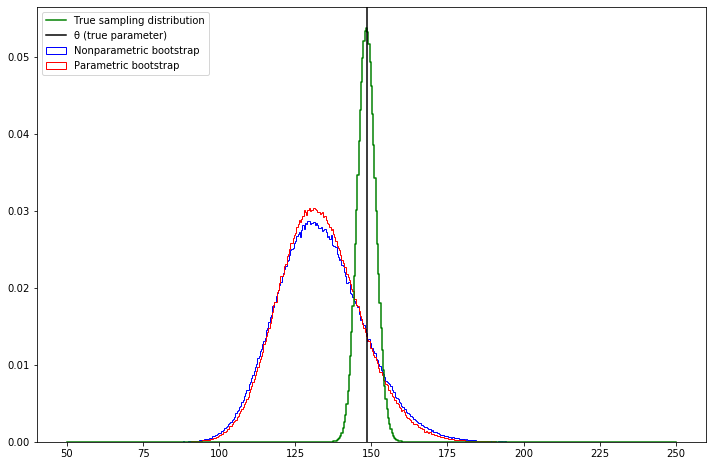
\includegraphics{Figure-09-02}
\end{figure}


\textbf{Exercise 9.6.7}. Let
\(X_{1}, \dots, X_{n} \sim \text{Uniform}(0, \theta)\). The mle is
\(\hat{\theta} = X_\text{max} = \max \{ X_{1}, \dots, X_{n} \}\). Generate a
dataset of size 50 with \(\theta = 1\).
\textbf{(a)} Find the distribution of \(\hat{\theta}\). Compare the true
distribution of \(\hat{\theta}\) to the histograms from the parametric
and nonparametric bootstraps.
\textbf{(b)} This is a case where the nonparametric bootstrap does very
poorly. In fact, we can prove that this is the case. Show that, for
parametric bootstrap \(\PROB(\hat{\theta}^{*} = \hat{\theta}) = 0\)
but for the nonparametric
\(\PROB(\hat{\theta}^{*} = \hat{\theta}) \approx 0.632\).
Hint: show that
\(\PROB(\hat{\theta}^{*} = \hat{\theta}) = 1 - (1 - (1/n))^{n}\) then
take the limit as \(n\) gets large.

\begin{python}
import numpy as np
X = np.random.uniform(low=0, high=1, size=50)
\end{python}

\begin{python}
# Nonparametric bootstrap
theta_hat = X.max()
B = 1000000
t_boot_nonparam = np.empty(B)
n = len(X)
for i in tqdm_notebook(range(B)):
    xx = np.random.choice(X, n, replace=True)
    t_boot_nonparam[i] = xx.max()
    
se_boot = t_boot_nonparam.std()
alpha = 0.05
z = norm.ppf(1 - alpha/2)
normal_conf = (theta_hat - z * se_boot, theta_hat + z * se_boot)
print('95%% confidence interval (Normal): \t %.3f, %.3f' % normal_conf)
\end{python}
\begin{console}
95\% confidence interval (Normal):        0.959, 1.037
\end{console}

\begin{python}
# Run parametric bootstrap
theta_hat = X.max()
B = 1000000
t_boot_param = np.empty(B)
n = len(X)
for i in tqdm_notebook(range(B)):
    xx = np.random.uniform(low=0, high=theta_hat, size=50)
    t_boot_param[i] = xx.max()
    
se_boot_param = t_boot_param.std()
alpha = 0.05
z = norm.ppf(1 - alpha/2)
normal_conf_param = (theta_hat - z * se_boot_param, theta_hat + z * se_boot_param)
print('95%% confidence interval (Parametric Normal): \t %.3f, %.3f' % normal_conf_param)
\end{python}
\begin{console}
95\% confidence interval (Parametric Normal):     0.960, 1.036
\end{console}
For the true sampling distribution,
\[
\hat{\theta} = \max \{ X_{1}, \dots X_{n} \}
\]
Its CDF is
\[
\PROB(\hat{\theta} \leq x) = \prod_{i=1}^{n} \PROB(X_{i} \leq x) = F_{\text{Uniform}(0, \theta)}(x)^{n}
\]
where
\[
F_{\text{Uniform}(0, \theta)}(x) = \begin{cases}
0 & \text{if } x \leq 0 \\
\frac{x}{\theta} & \text{if } 0 < x \leq \theta \\
1 & \text{if } \theta < x
\end{cases}
\]

\begin{python}
bins = np.linspace(0.75, 1.05, 200)
\end{python}

\begin{python}
# Generate the CDF for theta, calculate it for each bin, 
# and include the differences between bins
def theta_cdf(x):
    if x <= 0:
        return 0
    if x >= 1:
        return 1
    return x**50
theta_cdf_bins = list(map(theta_cdf, bins))
theta_cdf_bins_delta = np.empty(len(bins))
theta_cdf_bins_delta[0] = 0
theta_cdf_bins_delta[1:] = np.diff(theta_cdf_bins)
\end{python}

\begin{python}
plt.figure(figsize=(12, 8))
plt.hist(t_boot_nonparam, bins, label='Nonparametric bootstrap', color='blue', 
         histtype='step', density=True)
plt.hist(t_boot_param, bins, label='Parametric bootstrap', color='red', 
         histtype='step', density=True)
plt.axvline(x=1, color='black', label='θ (true parameter)')
plt.legend(loc='upper left')
plt.show()
\end{python}

\begin{figure}[H]
\centering
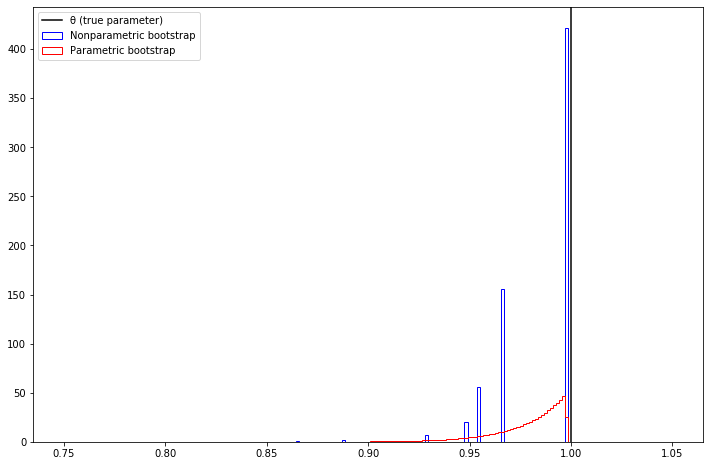
\includegraphics{Figure-09-03}
\end{figure}


\begin{python}
plt.figure(figsize=(12, 8))
plt.step(bins, theta_cdf_bins_delta, color='green', label='True sampling distribution')
plt.axvline(x=1, color='black', label='θ (true parameter)')
plt.legend(loc='upper left')
plt.ylim(0, 0.1)
plt.show()
\end{python}

\begin{figure}[H]
\centering
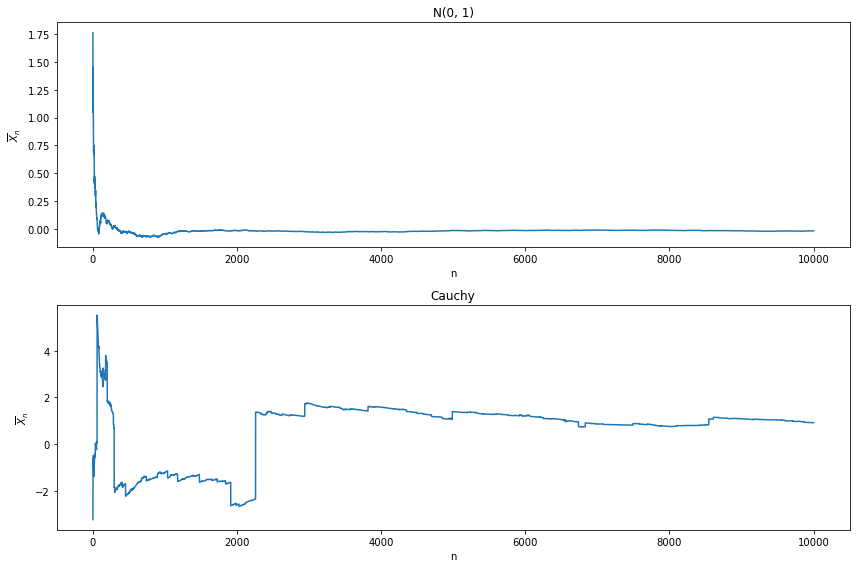
\includegraphics{Figure-04-01}
\end{figure}

\textbf{(b)}
For the parametric bootstrap process, the estimated parameter
\(\hat{\theta}^{*}\) is used on each \(k\)-th bootstrap sampling
\(\{ X_{k1}, X_{k2}, \dots, X_{kn} \}\). But each variable \(X_{kj}\) is
sampled from \(\text{Uniform}(0, \hat{\theta}^{*})\), which is a
continuous distribution -- so the probability of obtaining exactly a
sample at the boundaries is 0, and
\(\PROB(X_{kj} < \hat{\theta}^{*}) = 1\). Since the bootstrap
functional of each draw, \(T(F_{n}) = \max(F_{n})\) is the largest drawn
value in each sample, its values will also always be under
\(\hat{\theta}\), thus the estimated parameter via parametric
bootstraping will aywals be under \([\hat{\theta}\), and
\(\PROB(\hat{\theta}^{*} = \hat{\theta}) = 0\).
For the nonparametric bootstrap process, the estimated parameter
\(\hat{\theta}^{*}\) is the maximum value with a point mass in the
empirical distribution function \(\hat{F}\). Each bootstrap resample may
or may not include that value when drawing from this sample -- if
\(\max\{X_{1}, \dots, X_{n}\} \in \{X_{k1}, \dots, X_{kn} \}\) then the
estimated functional for that bootstrap sample will be the estimated
parameter \(\hat{\theta}^{*}\), otherwise it will necessarily be smaller.
Thus, the probability that \(\PROB(\hat{\theta}^{*} = \hat{\theta})\)
is the probability that the largest element on the original data is
included in a resampling with replacement. That turns out to be one
minus the probability that it never gets included, so,
\(\PROB(\hat{\theta}^{*} = \hat{\theta}) = 1 - (1 - (1/n))^{n}\). But
\(\lim_{n \rightarrow \infty } (1 + x/n)^{n} = e^x\), so the given
probability goes to \(1 - e^{-1} \approx 0.632\).

\textbf{Exercise 9.6.8}. Let \(T_{n} = \bar{X}_{n}^{2}\),
\(\mu = \EXP(X_{1})\), \(\alpha_{k} = \int |x - \mu|^{k} dF(x)\) and
\(\hat{\alpha}_{k} = n^{-1} \sum_{i=1}^{n} |X_{i} - \bar{X}_{n}|^{k}\). Show
that
\[
v_\text{boot} = \frac{4 \bar{X}_{n}^{2} \hat{\alpha}_{2}}{n} + \frac{4 \bar{X}_{n} \hat{\alpha}_{3}}{n^{2}} + \frac{\hat{\alpha}_{4}}{n^{3}}
\]

\textbf{Solution}.
First, we rewrite the sample mean in terms of an expression containing
the central moments. Let
\(S_{n} = n^{-1} \sum_{i=1}^{n} (X_{i} - \bar{X}_{n}) = 0\). Then:
\[
\bar{X}_{n} = S_{n} + \bar{X}_{n} = \frac{1}{n} \sum_{i=1}^{n} (X_{i} - \bar{X}_{n}) + \bar{X}_{n}
\]
The bootstrap variance, \(\VAR\left(\bar{X}_{n}^{2}\right)\), can
be expressed as
\[
\VAR\left(\bar{X}_{n}^{2}\right) = \EXP\left(\bar{X}_{n}^{4}\right) - \EXP\left(\bar{X}_{n}^{2}\right)^{2}
\]
Note that \(\bar{X}_{n}\) is the mean of the distribution, and can be
treated as constant when taking expectations.
We now have:
\begin{align*}
\EXP\left(\bar{X}_{n}^{4}\right) &= \EXP\left( (S_{n} + \bar{X}_{n})^{4} \right) \\
&= \EXP\left( S_{n}^{4} + 4 S_{n}^{3} \bar{X}_{n} + 6 S_{n}^{2} \bar{X}_{n}^{2} + 4 S_{n} \bar{X}_{n}^{3} + \bar{X}_{n}^{4} \right) \\
&= \EXP(S_{n}^{4}) + 4 \bar{X}_{n} \EXP(S_{n}^{3}) + 6 \bar{X}_{n}^{2} \EXP(S_{n}^{2}) + 4 \bar{X}_{n}^{3} \EXP(S_{n}) + \bar{X}_{n}^{4}
\end{align*}
Then, computing the moments of \(S_{n}\),
\begin{align*}
\EXP(S_{n}) &= 0 \\
\EXP(S_{n}^{2}) &= \EXP\left( n^{-2} \left( \sum_{i} X_{i} - \bar{X}_{n} \right)^{2} \right) = \frac{\hat{\alpha}_{2}}{n} \\
\EXP(S_{n}^{3}) &= \EXP\left( n^{-3} \left( \sum_{i} X_{i} - \bar{X}_{n} \right)^{3} \right) = \frac{\hat{\alpha}_{3}}{n^{2}} \\
\EXP(S_{n}^{4}) &= \EXP\left( n^{-4} \left( \sum_{i} X_{i} - \bar{X}_{n} \right)^{4} + n^{-2}n^{-4} \sum_{i} \sum_{j \neq i} (X_{i} - \bar{X}_{n})^{2} (X_{j} - \bar{X}_{n})^{2} \right) = \frac{\hat{\alpha}_{4} + \hat{\alpha}_{2}^{2}}{n^{3}}
\end{align*}
and finally
\[
\EXP\left(\bar{X}_{n}^{2}\right)^{2} = \EXP\left(\bar{X}_{n}^{2} + S_{n}\right)^{2} = \bar{X}_{n}^{4} + 2 \bar{X}_{n}^{2} \frac{\hat{\alpha}_{2}}{n} + \frac{\hat{\alpha}_{2}^{2}}{n^{2}}
\]
Putting everything together,
\begin{align*}
v_\text{boot} &= \EXP\left( (S_{n} + \bar{X}_{n})^{4} \right) - \EXP\left(\bar{X}_{n}^{2} + S_{n}\right)^{2} \\
&= \EXP(S_{n}^{4}) + 4 \bar{X}_{n} \EXP(S_{n}^{3}) + 6 \bar{X}_{n}^{2} \EXP(S_{n}^{2}) + 4 \bar{X}_{n}^{3} \EXP(S_{n}) + \bar{X}_{n}^{4} - \left( \bar{X}_{n}^{4} + 2 \bar{X}_{n}^{2} \frac{\hat{\alpha}_{2}}{n} + \frac{\hat{\alpha}_{2}^{2}}{n^{2}}\right) \\
&= \frac{\hat{\alpha}_{4} + \hat{\alpha}_{2}^{2}}{n^{3}} + 4 \bar{X}_{n} \frac{\hat{\alpha}_{3}}{n^{2}} + 6 \bar{X}_{n}^{2} \frac{\hat{\alpha}_{2}}{n} + 0 + \bar{X}_{n}^{4} - \bar{X}_{n}^{4} - 2 \bar{X}_{n}^{2} \frac{\hat{\alpha}_{2}}{n} - \frac{\hat{\alpha}_{2}^{2}}{n^{2}} \\
&= \frac{4 \bar{X}_{n}^{2} \hat{\alpha}_{2}}{n} + \frac{4 \bar{X}_{n} \hat{\alpha}_{3}}{n^{2}} + \frac{\hat{\alpha}_{4}}{n^{3}}
\end{align*}
Reference and discussion: \url{https://stats.stackexchange.com/q/26082}


% Chapter 10
\section*{10. Parametric Inference}\label{parametric-inference}

\textbf{Parametric models} are of the form

\[ \mathfrak{F} = \bigg\{ f(x; \theta) : \; \theta \in \Theta \bigg\} \]

where \(\Theta \subset \mathbb{R}^{k}\) is the parameter space and
\(\theta = (\theta_{1}, \dots, \theta_{k})\) is the parameter. The problem
of inference then reduces to the problem of estimating parameter
\(\theta\).

\subsection*{10.1 Parameter of interest}\label{parameter-of-interest}

Often we are only interested in some function \(T(\theta)\). For
example, if \(X \sim N(\mu, \sigma^{2})\) then the parameter is
\(\theta = (\mu, \sigma)\). If our goal is to estimate \(\mu\) then
\(\mu = T(\theta)\) is called the \textbf{parameter of interest} and
\(\sigma\) is called a \textbf{nuisance parameter}.

\subsection*{10.2 The Method of Moments}\label{the-method-of-moments}

Suppose that the parameter \(\theta = (\theta_{1}, \dots, \theta_{n})\) has
\(k\) components. For \(1 \leq j \leq k\) define the \(j\)-th
\textbf{moment}

\[ \alpha_{j} \equiv \alpha_{j}(\theta) = \mathbb{E}_\theta(X^{j}) = \int x^{j} dF_\theta(x)\]

and the \(j\)-th \textbf{sample moment}

\[ \hat{\alpha}_{j} = \frac{1}{n} \sum_{i=1}^{n} X_{i}^{j} \]

The \textbf{method of moments estimator} \(\hat{\theta}_{n}\) is defined
to be the value of \(\theta\) such that

\begin{align*}
\alpha_{1}(\hat{\theta}_{n}) &= \hat{\alpha_{1}} \\
\alpha_{2}(\hat{\theta}_{n}) &= \hat{\alpha_{2}} \\
\vdots \\
\alpha_{k}(\hat{\theta}_{n}) &= \hat{\alpha_{k}}  
\end{align*}

This defines a system of \(k\) equations with \(k\) unknowns.

\textbf{Theorem 10.6}. Let \(\hat{\theta}_{n}\) denote the method of
moments estimator. Under the conditions given in the appendix, the
following statements hold:

\begin{enumerate}
\def\labelenumi{(\arabic{enumi})}
\item
  The estimate \(\hat{\theta}_{n}\) exists with probability tending to 1.
\item
  The estimate is consistent:
  \(\hat{\theta}_{n} \xrightarrow{\text{P}} \theta\).
\item
  The estimate is asymptotically Normal:
\end{enumerate}

\[\sqrt(n)(\hat{\theta}_{n} - \theta) \leadsto N(0, \Sigma) \]

where

\[
\Sigma = g \mathbb{E}_\theta (Y Y^T) g^T \\
Y = (X, X^{2}, \dots, X^{k})^T, \quad g = (g_{1}, \dots, g_{k}) \quad \text{and} \quad g_{j} = \partial \alpha_{j}^{-1}(\theta)/\partial\theta
\]

The last statement in Theorem 10.6 can be used to find standard errors
and confidence intervals. However, there is an easier way: the
bootstrap.

\subsection*{10.3 Maximum Likelihood}\label{maximum-likelihood}

Let \(X_{1}, \dots, X_{n}\) be iid with PDF \(f(x; \theta)\).

The \textbf{likelihood function} is defined by

\[ \mathcal{L}_{n}(\theta) = \prod_{i=1}^{n} f(X_{i}; \theta) \]

The \textbf{log-likelihood function} is defined by
\(\ell_{n}(\theta) = \log \mathcal{L}_{n}(\theta)\).

The likelihood function is just the joint density of the data, except we
treat is as a function of parameter \(\theta\). Thus
\(\mathcal{L}_{n} : \Theta \rightarrow [0, \infty)\). The likelihood
function is not a density function; in general it is not true that
\(\mathcal{L}_{n}\) integrates to 1.

The \textbf{maximum likelihood estimator} MLE, denoted by
\(\hat{\theta}_{n}\), is the value of \(\theta\) that maximizes
\(\mathcal{L}_{n}(\theta)\).

The maximum of \(\ell_{n}(\theta)\) occurs at the same place as the
maximum of \(\mathcal{L}_{n}(\theta)\), so maximizing either leads to the
same answer. Often it is easier to maximize the log-likelihood.

\subsection*{10.4 Properties of Maximum Likelihood
Estimators}\label{properties-of-maximum-likelihood-estimators}

Under certain conditions on the model, the MLE \(\hat{\theta}_{n}\)
possesses many properties that make it an appealing choice of estimator.

The main properties of the MLE are:

\begin{itemize}[tightlist]
\item
  It is \textbf{consistent}:
  \(\hat{\theta}_{n} \xrightarrow{\text{P}} \theta_*\), where \(\theta_*\)
  denotes the true value of parameter \(\theta\).
\item
  It is \textbf{equivariant}: if \(\hat{\theta}_{n}\) is the MLE of
  \(\theta\) then \(g(\hat{\theta}_{n})\) is the MLE of \(g(\theta)\).
\item
  If is \textbf{asymptotically Normal}:
  \(\sqrt{n}(\hat{\theta} - \theta_*) / \hat{\text{se}} \leadsto N(0, 1)\)
  where \(\hat{\text{se}}\) can be computed analytically.
\item
  It is \textbf{asymptotically optimal} or \textbf{efficient}: roughly,
  this means that among all well behaved estimators, the MLE has the
  smallest variance, at least for large samples.
\item
  The MLE is approximately the Bayes estimator.
\end{itemize}

\subsection*{10.5 Consistency of Maximum Likelihood
Estimator}\label{consistency-of-maximum-likelihood-estimator}

If \(f\) and \(g\) are PDFs, define the \textbf{Kullback-Leibler
distance} between \(f\) and \(g\) to be:

\[ D(f, g) = \int f(x) \log \left( \frac{f(x)}{g(x)} \right) dx \]

It can be shown that \(D(f, g) \geq 0\) and \(D(f, f) = 0\). For any
\(\theta, \psi \in \Theta\) write \(D(\theta, \psi)\) to mean
\(D(f(x; \theta), f(x; \psi))\). We will assume that
\(\theta \neq \psi\) implies \(D(\theta, \psi) > 0\).

Let \(\theta_*\) denote the true value of \(\theta\). Maximizing
\(\ell_{n}(\theta)\) is equivalent to maximizing

\[M_{n}(\theta) = \frac{1}{n} \sum_{i} \log \frac{f(X_{i}; \theta)}{f(X_{i}; \theta_*)}\]

By the law of large numbers, \(M_{n}(\theta)\) converges to:

\begin{align*}
\mathbb{E}_{\theta_*} \left( \log \frac{f(X_{i}; \theta)}{f(X_{i}; \theta_*)} \right)
& = \int \log \left( \frac{f(x; \theta)}{f(x; \theta_*)} \right) f(x; \theta_*) dx \\
& = - \int \log \left( \frac{f(x; \theta_*)}{f(x; \theta)} \right) f(x; \theta_*) dx \\
&= -D(\theta_*, \theta)
\end{align*}

Hence \(M_{n}(\theta) \approx -D(\theta_*, \theta)\) which is maximized at
\(\theta_*\), since the KL distance is 0 when \(\theta_* = \theta\) and
positive otherwise. Hence, we expect that the maximizer will tend to
\(\theta_*\).

To prove this formally, we need more than
\(M_{n}(\theta) \xrightarrow{\text{P}} -D(\theta_*, \theta)\). We need
this convergence to be uniform over \(\theta\). We also have to make
sure that the KL distance is well-behaved. Here are the formal details.

\textbf{Theorem 10.13}. Let \(\theta_*\) denote the true value of
\(\theta\). Define

\[M_{n}(\theta) = \frac{1}{n} \sum_{i} \log \frac{f(X_{i}; \theta)}{f(X_{i}; \theta_*)}\]

and \(M(\theta) = -D(\theta_*, \theta)\). Suppose that

\[ \sup _{\theta \in \Theta} |M_{n}(\theta) - M(\theta)| \xrightarrow{\text{P}} 0 \]

and that, for every \(\epsilon > 0\),

\[ \sup _{\theta : |\theta - \theta_*| \geq \epsilon} M(\theta) < M(\theta_*)\]

Let \(\hat{\theta}_{n}\) denote the mle. Then
\(\hat{\theta}_{n} \xrightarrow{\text{P}} \theta_*\).

\subsection*{10.6 Equivalence of the
MLE}\label{equivalence-of-the-mle}

\textbf{Theorem 10.14}. Let \(\tau = g(\theta)\) be a one-to-one
function of \(\theta\). Let \(\hat{\theta}_{n}\) be the MLE of \(\theta\).
Then \(\hat{\tau}_{n} = g(\hat{\theta}_{n})\) is the MLE of \(\tau\).

\textbf{Proof}. Let \(h = g^{-1}\) denote the inverse of \(g\). Then
\(\hat{\theta}_{n} = h(\hat{\tau}_{n})\). For any \(\tau\),
\(L(\tau) = \prod_{i} f(x_{i}; h(\tau)) = \prod_{i} f(x_{i}; \theta) = \mathcal{L}(\theta)\)
where \(\theta = h(\tau)\). Hence, for any \(\tau\),
\(\mathcal{L}_{n}(\tau) = \mathcal{L}(\theta) \leq \mathcal{L}(\hat{\theta}) = \mathcal{L}_{n}(\hat{\tau})\).

\subsection*{10.7 Asymptotic Normality}\label{asymptotic-normality}

The \textbf{score function} is defined to be

\[ s(X; \theta) = \frac{\partial \log f(X; \theta)}{\partial \theta} \]

The \textbf{Fisher information} is defined to be

\begin{align*}
I_{n}(\theta) &= \mathbb{V}_\theta \left( \sum_{i=1}^{n} s(X_{i}; \theta) \right) \\
&= \sum_{i=1}^{n} \mathbb{V}_\theta(s(X_{i}; \theta))
\end{align*}

For \(n = 1\) we sometimes write \(I(\theta)\) instead of
\(I_{1}(\theta)\).

It can be shown that \(\mathbb{E}_\theta(s(X; \theta)) = 0\). It then
follows that
\(\mathbb{V}_\theta(s(X; \theta)) = \mathbb{E}_\theta((s(X; \theta))^{2})\).
A further simplification of \(I_{n}(\theta)\) is given in the next result.

\textbf{Theorem 10.17}.

\[ I_{n}(\theta) = n I(\theta)\]

\begin{align*}
I(\theta) & = -\mathbb{E}_\theta \left( \frac{\partial^{2} \log f(X; \theta)}{\partial^{2} \theta^{2}} \right) \\
&= - \int \left( \frac{\partial^{2} \log f(x; \theta)}{\partial^{2} \theta^{2}} \right) f(x; \theta) dx
\end{align*}

\textbf{Theorem 10.18 (Asymptotic Normality of the MLE)}. Under
appropriate regularity conditions, the following hold:

\begin{enumerate}[tightlist,label={\arabic*.}]
\item
  Let \(\text{se} = \sqrt{1 / I_{n}(\theta)}\). Then,
\end{enumerate}

\[ \frac{\hat{\theta}_{n} - \theta}{\text{se}} \leadsto N(0, 1) \]

\begin{enumerate}[tightlist,label={\arabic*.}]
\item
  Let \(\hat{\text{se}} = \sqrt{1 / I_{n}(\hat{\theta}_{n})}\). Then,
\end{enumerate}

\[ \frac{\hat{\theta}_{n} - \theta}{\hat{\text{se}}} \leadsto N(0, 1) \]

The first statement says that
\(\hat{\theta}_{n} \approx N(\theta, \text{se})\). The second statement
says that this is still true if we replace the standard error
\(\text{se}\) by its estimated standard error \(\hat{\text{se}}\).

Informally this says that the distribution of the MLE can be
approximated with \(N(\theta, \hat{\text{se}})\). From this fact we can
construct an asymptotic confidence interval.

\textbf{Theorem 10.19}. Let

\[ C_{n} = \left( \hat{\theta_{n}} - z_{\alpha/2} \hat{\text{se}}, \; \hat{\theta_{n}} + z_{\alpha/2} \hat{\text{se}} \right) \]

Then, \(\mathbb{P}_\theta(\theta \in C_{n}) \rightarrow 1 - \alpha\) as
\(n \rightarrow \infty\).

\textbf{Proof} Let \(Z\) denote a standard random variable. Then,

\begin{align*}
\mathbb{P}_\theta(\theta \in C_{n}) 
&= \mathbb{P}_\theta(\hat{\theta}_{n} - z_{\alpha/2} \hat{\text{se}} \leq \theta \leq \hat{\theta}_{n} + z_{\alpha/2} \hat{\text{se}}) \\
&= \mathbb{P}_\theta(-z_{\alpha/2} \leq \frac{\hat{\theta}_{n} - \theta}{\hat{\text{se}}} \leq z_{\alpha/2}) \\
&\rightarrow \mathbb{P}(-z_{\alpha/2} \leq Z \leq z_{\alpha/2}) = 1 - \alpha
\end{align*}

\subsection*{10.8 Optimality}\label{optimality}

Suppose that \(X_{1}, \dots, X_{n} \sim N(0, \sigma^{2})\). The MLE is
\(\hat{\theta}_{n} = \overline{X}_{n}\). Another reasonable estimator is the
sample median \(\overline{\theta}_{n}\). The MLE satisfies

\[ \sqrt{n}(\hat{\theta}_{n} - \theta) \leadsto N(0, \sigma^{2}) \]

It can be proved that the median satisfies

\[ \sqrt{n}(\overline{\theta}_{n} - \theta) \leadsto N\left(0, \sigma^{2} \frac{\pi}{2} \right) \]

This means that the median converges to the right value but has a larger
variance than the MLE.

More generally, consider two estimators \(T_{n}\) and \(U_{n}\) and suppose
that

\[
\sqrt{n}(T_{n} - \theta) \leadsto N(0, t^{2}) 
\quad \text{and} \quad 
\sqrt{n}(U_{n} - \theta) \leadsto N(0, u^{2})
\]

We define the \textbf{asymptotic relative efficiency} of U to T by
\(ARE(U, T) = t^{2}/u^{2}\). In the Normal example,
\(ARE(\overline{\theta}_{n}, \hat{\theta}_{n}) = 2 / \pi = 0.63\).

\textbf{Theorem 10.23}. If \(\hat{\theta}_{n}\) is the MLE and
\(\overline{\theta}_{n}\) is any other estimator then

\[ ARE(\overline{\theta}_{n}, \hat{\theta}_{n}) \leq 1 \]

Thus, MLE has the smallest (asymptotic) variance and we say that MLE is
\textbf{efficient} or \textbf{asymptotically optimal}.

The result is predicated over the model being correct -- otherwise the
MLE may no longer be optimal.

\subsection*{10.9 The Delta Method}\label{delta:method}

Let \(\tau = g(\theta)\) where \(g\) is a smooth function. The maximum
likelihood estimator of \(\tau\) is \(\hat{\tau} = g(\hat{\theta})\).

\textbf{Theorem 10.24 (The Delta Method)}. If \(\tau = g(\theta)\) where
\(g\) is differentiable and \(g'(\theta) \neq 0\) then

\[ \frac{\sqrt{n}(\hat{\tau}_{n} - \tau)}{\hat{\text{se}}(\hat{\tau})} \leadsto N(0, 1) \]

where \(\hat{\tau}_{n} = g(\hat{\theta})\) and

\[ \hat{\text{se}}(\hat{\tau}_{n}) = |g'(\hat{\theta})| \hat{\text{se}} (\hat{\theta}_{n}) \]

Hence, if

\[ C_{n} = \left( \hat{\tau}_{n} - z_{\alpha/2} \hat{\text{se}}(\hat{\tau}_{n}), \; \hat{\tau}_{n} + z_{\alpha/2} \hat{\text{se}}(\hat{\tau}_{n}) \right) \]

then \(\mathbb{P}_\theta(\tau \in C_{n}) \rightarrow 1 - \alpha\) as
\(n \rightarrow \infty\).

\subsection*{10.10 Multiparameter Models}\label{multiparameter-models}

We can extend these ideas to models with several parameters.

Let \(\theta = (\theta_{1}, \dots, \theta_{n})\) and let
\(\hat{\theta} = (\hat{\theta}_{1}, \dots, \hat{\theta}_{n})\) be the MLE.
Let \(\ell_{n} = \sum_{i=1}^{n} \log f(X_{i}; \theta)\),

\[
H_{j}j = \frac{\partial^{2} \ell_{n}}{\partial \theta_{j}^{2}}
\quad \text{and} \quad
H_{j}k = \frac{\partial^{2} \ell_{n}}{\partial \theta_{j} \partial \theta_{k}}
\]

Define the \textbf{Fisher Information Matrix} by

\[
I_{n}(\theta) = -
\begin{bmatrix}
\mathbb{E}_\theta(H_{11}) & \mathbb{E}_\theta(H_{12}) & \cdots & \mathbb{E}_\theta(H_{1k}) \\
\mathbb{E}_\theta(H_{21}) & \mathbb{E}_\theta(H_{22}) & \cdots & \mathbb{E}_\theta(H_{2k}) \\
\vdots & \vdots & \ddots & \vdots \\
\mathbb{E}_\theta(H_{k1}) & \mathbb{E}_\theta(H_{k2}) & \cdots & \mathbb{E}_\theta(H_{kk})
\end{bmatrix}
\]

Let \(J_{n}(\theta) = I_{n}^{-1}(\theta)\) be the inverse of \(I_{n}\).

\textbf{Theorem 10.27}. Under appropriate regularity conditions,

\[ \sqrt(n)(\hat{\theta} - \theta) \approx N(0, J_{n}(\theta))\]

Also, if \(\hat{\theta}_{j}\) is the \(j\)-th component of
\(\hat{\theta}\), then

\[ \frac{\sqrt{n}(\hat{\theta_{j}} - \theta_{j})}{\hat{\text{se}}_{j}} \approx N(0, 1) \]

where \(\hat{\text{se}}_{j}^{2}\) is the \(j\)-th diagonal element of
\(J_{n}\). The approximate covariance of \(\hat{\theta}_{j}\) and
\(\hat{\theta}_{k}\) is
\(\text{Cov}(\hat{\theta}_{j}, \hat{\theta}_{k}) \approx J_{n}(j, k)\).

There is also a multiparameter delta method. Let
\(\tau = g(\theta_{1}, \dots, \theta_{k})\) be a function and let

\[ \nabla g = \begin{pmatrix}
\frac{\partial g}{\partial \theta_{1}} \\
\vdots \\
\frac{\partial g}{\partial \theta_{k}}
\end{pmatrix}
\]

be the gradient of \(g\).

\textbf{Theorem 10.28 (Multiparameter delta method)}. Suppose that
\(\nabla g\) evaluated at \(\hat{\theta}\) is not 0. Let
\(\hat{\tau} = g(\hat{\theta})\). Then

\[ \frac{\sqrt{n}(\hat{\tau} - \tau)}{\hat{\text{se}}(\hat{\tau})} \leadsto N(0, 1) \]

where

\[ \hat{\text{se}}(\hat{\tau}) = \sqrt{\left(\hat{\nabla} g \right)^T \hat{J}_{n} \left(\hat{\nabla} g \right)} ,\]

\(\hat{J}_{n} = J_{n}(\hat{\theta}_{n})\) and \(\hat{\nabla}g\) is
\(\nabla g\) evaluated at \(\theta = \hat{\theta}\).

\subsection*{10.11 The Parametric
Bootstrap}\label{the-parametric-bootstrap}

For parametric models, standard errors and confidence intervals may also
be estimated using the bootstrap. There is only one change. In
nonparametric bootstrap, we sampled \(X_{1}^*, \dots, X_{n}*\) from the
empirical distribution \(\hat{F}_{n}\). In the parametric bootstrap we
sample instead from \(f(x; \hat{\theta}_{n})\). Here, \(\hat{\theta}_{n}\)
could be the MLE or the method of moments estimator.

\subsection*{10.12 Technical Appendix}

\paragraph{10.12.1 Proofs}\label{proofs}

\textbf{Proof of Theorem 10.13}. Since \(\hat{\theta}_{n}\) maximizes
\(M_{n}(\theta)\), we have \(M_{n}(\hat{\theta}) \geq M_{n}(\theta_*)\).
Hence,

\begin{align*}
M(\theta_*) - M(\hat{\theta}_{n}) 
&= M_{n}(\theta_*) - M(\hat{\theta}_{n}) + M(\hat{\theta}_*) - M_{n}(\theta_*) \\
&\leq M_{n}(\hat{\theta}) - M(\hat{\theta}_{n}) + M(\theta_*) - M_{n}(\theta_*) \\
&\leq \sup_\theta | M_{n}(\theta) - M(\theta) |  + M(\theta_*)  - M_{n}(\theta_*) \\
&\xrightarrow{\text{P}} 0
\end{align*}

It follows that, for any \(\delta > 0\),

\[\mathbb{P}(M(\hat{\theta}_{n}) < M(\theta_*) - \delta) \rightarrow 0\]

Pick any \(\epsilon > 0\). There exists \(\delta > 0\) such that
\(|\theta - \theta_*| \geq \epsilon\) implies that
\(M(\theta) < M(\theta_*) - \delta\). Hence,

\[\mathbb{P}(|\hat{\theta}_{n} - \theta_*| > \epsilon) \leq 
\mathbb{P}\left( M(\hat{\theta}_{n}) < M(\theta_*) - \delta \right) \rightarrow 0\]

\textbf{Lemma 10.31}. The score function satisfies

\[\mathbb{E}[s(X; \theta)] = 0\]

\textbf{Proof}. Note that \(1 = \int f(x; \theta) dx\). Differentiate
both sides of this equation to get

\begin{align*}
0 &= \frac{\partial}{\partial \theta} \int f(x; \theta)dx = \int \frac{\partial}{\partial \theta} f(x; \theta) dx \\
&= \int \frac{\frac{\partial f(x; \theta)}{\partial \theta}}{f(x; \theta)} f(x; \theta) dx
= \int \frac{\partial \log f(x; \theta)}{\partial \theta} f(x; \theta) dx \\
&= \int s(x; \theta) f(x; \theta) dx = \mathbb{E}[s(X; \theta)]
\end{align*}

\textbf{Proof of Theorem 10.18}. Let
\(\ell(\theta) = \log \mathcal{L}(\theta)\). Then

\[0 = \ell'(\hat{\theta}) \approx \ell'(\theta) + (\hat{\theta} - \theta) \ell''(\theta)\]

Rearrange the above equation to get
\(\hat{\theta} - \theta = -\ell'(\theta) / \ell''(\theta)\), or

\[ \sqrt{n}(\hat{\theta} - \theta) = \frac{\frac{1}{\sqrt{n}}\ell'(\theta)}{-\frac{1}{n}\ell''(\theta)} = \frac{\text{TOP}}{\text{BOTTOM}}\]

Let \(Y_{i} = \partial \log f(X_{i}, \theta) / \partial \theta\). From the
previous lemma \(\mathbb{E}(Y_{i}) = 0\) and also
\(\mathbb{V}(Y_{i}) = I(\theta)\). Hence,

\[\text{TOP} = n^{-1/2} \sum_{i} Y_{i} = \sqrt{n} \overline{Y} = \sqrt{n} (\overline{Y} - 0) \leadsto W \sim N(0, I)\]

by the central limit Theorem. Let
\(A_{i} = -\partial^{2} \log f(X_{i}; \theta) / \partial theta^{2}\). Then
\(\mathbb{E}(A_{i}) = I(\theta)\) and

\[\text{BOTTOM} = \overline{A} \xrightarrow{\text{P}} I(\theta)\]

by the law of large numbers. Apply Theorem 6.5 part (e) to conclude that

\[\sqrt{n}(\hat{\theta} - \theta) \leadsto \frac{W}{I(\theta)} \sim N \left(0, \frac{1}{I(\theta)} \right)\]

Assuming that \(I(\theta)\) is a continuous function of \(\theta\), it
follows that \(I(\hat{\theta}_{n}) \xrightarrow{\text{P}} I(\theta)\). Now

\begin{align*}
\frac{\hat{\theta}_{n} - \theta}{\hat{\text{se}}}&= \sqrt{n} I^{1/2}(\hat{\theta_{n}})(\hat{\theta_{n}} - \theta) \\
&= \left\{ \sqrt{n} I^{1/2}(\theta)(\hat{\theta}_{n} - \theta)\right\} \left\{ \frac{I(\hat{\theta}_{n})}{I(\theta)} \right\}^{1/2}
\end{align*}

The first term tends in distribution to \(N(0, 1)\). The second term
tends in probability to 1. The result follows from Theorem 6.5 part (e).

\textbf{Outline of proof of Theorem 10.24}. Write,

\[\hat{\tau} = g(\hat{\theta}) \approx g(\theta) + (\hat{\theta} - \theta)g'(\theta) = \tau + (\hat{\theta} - \theta)g'(\theta)\]

Thus,

\[\sqrt{n}(\hat{\tau} - \tau) \approx \sqrt{n}(\hat{\theta} - \theta)g'(\theta)\]

and hence

\[\frac{\sqrt{n}I^{1/2}(\theta)(\hat{\theta} - \theta)}{g'(\theta)} \approx \sqrt{n}I^{1/2}(\theta)(\hat{\theta} - \theta)\]

Theorem 10.18 tells us that the right hand side tends in distribution to
\(N(0, 1)\), hence

\[\frac{\sqrt{n}I^{1/2}(\theta)(\hat{\theta} - \theta)}{g'(\theta)} \leadsto N(0, 1)\]

or, in other words,

\[\hat{\tau} \approx N(\tau, \text{se}^{2}(\hat{\tau}_{n}))\]

where

\[\text{se}^{2}(\hat{\tau}_{n}) = \frac{(g'(\theta))^{2}}{nI(\theta)}\]

The result remains true if we substitute \(\hat{\theta}\) for \(\theta\)
by Theorem 6.5 part (e).

\paragraph{10.12.2 Sufficiency}\label{sufficiency}

A \textbf{statistic} is a function \(T(X^{n})\) of the data. A sufficient
statistic is a statistic that contains all of the information in the
data.

Write \(x^{n} \leftrightarrow y^{n}\) if
\(f(x^{n}; \theta) = c f(y^{n}; \theta)\) for some constant \(c\) that might
depend on \(x^{n}\) and \(y^{n}\) but not \(\theta\). A statistic is
\textbf{sufficient} if \(T(x^{n}) \leftrightarrow T(y^{n})\) implies that
\(x^{n} \leftrightarrow y^{n}\).

Notice that if \(x^{n} \leftrightarrow y^{n}\) then the likelihood functions
based on \(x^{n}\) and \(y^{n}\) have the same shape. Roughly speaking, a
statistic is sufficient if we can calculate the likelihood function
knowing only \(T(X^{n})\).

A statistic \(T\) is \textbf{minimally sufficient} if it is sufficient
and it is a function of every other sufficient statistic.

\textbf{Theorem 10.36}. \(T\) is minimally sufficient if
\(T(x^{n}) = T(y^{n})\) if and only if \(x^{n} \leftrightarrow y^{n}\).

The usual definition of sufficiency is this: \(T\) is sufficient if the
distribution of \(X^{n}\) given \(T(X^{n}) = t\) does not depend on
\(\theta\).

\textbf{Theorem 10.40 (Factorization Theorem)}. \(T\) is sufficient if
and only if there are functions \(g(t, \theta)\) and \(h(x)\) such that
\(f(x^{n}; \theta) = g(t(x^{n}); \theta)h(x^{n})\).

\textbf{Theorem 10.42 (Rao-Blackwell)}. Let \(\hat{\theta}\) be an
estimator and let \(T\) be a sufficient statistic. Define a new
estimator by

\[\overline{\theta} = \mathbb{E}(\hat{\theta} | T)\]

Then, for every \(\theta\),

\[R(\theta, \overline{\theta}) \leq R(\theta, \hat{\theta})\]

where
\(R(\theta, \hat{\theta}) = \mathbb{E}_\theta[(\theta - \hat{\theta})^{2}]\)
denote the MSE of an estimator.

\paragraph{10.12.3 Exponential Families}\label{exponential-families}

We say that \(\{f(x; \theta) : \theta \in \Theta\}\) is a
\textbf{one-parameter exponential family} if there are functions
\(\eta(\theta)\), \(B(\theta)\), \(T(x)\) and \(h(x)\) such that

\[f(x; \theta) = h(x) e^{\eta(\theta)T(x) - B(\theta)}\]

It is easy to see that \(T(X)\) is sufficient. We call \(T\) the
\textbf{natural sufficient statistic}.

We can rewrite an exponential family as

\[f(x; \eta) = h(x) e^{\eta T(x) - A(\eta)}\]

where \(\eta = \eta(\theta)\) is called the \textbf{natural parameter}
and

\[A(\eta) = \log \int h(x) e^{\eta T(x)} dx\]

Let \(X_{1}, \dots, X_{n}\) be iid from an exponential family. Then
\(f(x^{n}; \theta)\) is an exponential family:

\[f(x^{n}; \theta) = h_{n}(x^{n}) e^{\eta(\theta) T_{n}(x^{n}) - B_{n}(\theta)}\]

where \(h_{n}(x^{n}) = \prod_{i} h(x_{i})\), \(T_{n}(x^{n}) = \sum_{i} T(x_{i})\) and
\(B_{n}(\theta) = nB(\theta)\). This implies that \(\sum_{i} T(X_{i})\) is
sufficient.

\textbf{Theorem 10.47}. Let \(X\) have an exponential family. Then,

\[
\mathbb{E}(T(X)) = A'(\eta),
\quad
\mathbb{V}(T(X)) = A''(\eta)
\]

If \(\theta = (\theta_{1}, \dots, \theta_{n})\) is a vector, then we say
that \(f(x; \theta)\) has exponential family form if

\[ f(x; \theta) = h(x) \exp \left\{ \sum_{j=1}^{k} \eta_{j}(\theta) T_{j}(x) - B(\theta) \right\}\]

Again, \(T = (T_{1}, \dots, T_{k})\) is sufficient and \(n\) iid samples
also has exponential form with sufficient statistic
\(\left(\sum_{i} T_{1}(X_{i}), \dots, \sum_{i} T_{k}(X_{i})\right)\).

\section*{10.13 Exercises}

\textbf{Exercise 10.13.1}. Let
\(X_{1}, \dots, X_{n} \sim \text{Gamma}(\alpha, \beta)\). Find the method of
moments estimator for \(\alpha\) and \(\beta\).

\textbf{Solution}.

The first two moments are:

\[
\alpha_{1} = \mathbb{E}(X) = \frac{\alpha}{\beta}\\
\alpha_{2} = \mathbb{E}(X^{2}) = \mathbb{V}(X) + \mathbb{E}(X)^{2} = \frac{\alpha}{\beta^{2}} + \frac{\alpha^{2}}{\beta^{2}} = \frac{\alpha(\alpha + 1)}{\beta^{2}} 
\]

We have the sample moments:

\[\hat{\alpha}_{1} = \frac{1}{n}\sum_{i=1}^{n} X_{i}
\quad \quad
\hat{\alpha}_{2} = \frac{1}{n}\sum_{i=1}^{n} X_{i}^{2}\]

Equating these we get:

\[
\hat{\alpha}_{1} = \frac{\hat{\alpha}_{n}}{\hat{\beta}_{n}}
\quad \quad
\hat{\alpha}_{2} = \frac{\hat{\alpha}_{n}(\hat{\alpha}_{n} + 1)}{\hat{\beta}_{n}^{2}}
\]

Solving these we get the method of moments estimators for \(\alpha\) and
\(\beta\):

\[
\hat{\alpha}_{n} = \frac{\hat{\alpha}_{1}^{2}}{\hat{\alpha}_{2} - \hat{\alpha}_{1}^{2}}
\quad \quad
\hat{\beta}_{n} = \frac{\hat{\alpha}_{1}}{\hat{\alpha}_{2} - \hat{\alpha}_{1}^{2}}
\]

\textbf{Exercise 10.13.2}. Let
\(X_{1}, \dots, X_{n} \sim \text{Uniform}(a, b)\) where \(a, b\) are unknown
parameters and \(a < b\).

\textbf{(a)} Find the method of moments estimators for \(a\) and \(b\).

\textbf{(b)} Find the MLE \(\hat{a}\) and \(\hat{b}\).

\textbf{(c)} Let \(\tau = \int x dF(x)\). Find the MLE of \(\tau\).

\textbf{(d)} Let \(\hat{\tau}\) be the MLE from the previous item. Let
\(\tilde{\tau}\) be the nonparametric plug-in estimator of
\(\tau = \int x dF(x)\). Suppose that \(a = 1\), \(b = 3\) and
\(n = 10\). Find the MSE of \(\hat{\tau}\) by simulation. Find the MSE
of \(\tilde{\tau}\) analytically. Compare.

\textbf{Solution}.

\textbf{(a)}

The first two moments are:

\[ 
\alpha_{1} = \mathbb{E}(X) = \frac{a + b}{2} \\
\alpha_{2} = \mathbb{E}(X^{2}) = \mathbb{V}(X) + \mathbb{E}(X)^{2} = \frac{(b - a)^{2}}{12} + \frac{(a + b)^{2}}{4}
= \frac{a^{2} + ab + b^{2}}{3}
\]

We have the sample moments:

\[\hat{\alpha}_{1} = \frac{1}{n}\sum_{i=1}^{n} X_{i}
\quad \quad
\hat{\alpha}_{2} = \frac{1}{n}\sum_{i=1}^{n} X_{i}^{2}\]

Equating these we get:

\[
\hat{\alpha}_{1} = \frac{\hat{a} + \hat{b}}{2}
\quad \quad
\hat{\alpha}_{2} = \frac{(\hat{b} - \hat{a})^{2}}{12} + \frac{(\hat{a} + \hat{b})^{2}}{4}
\]

Solving these we get the method of moment estimators for \(a\) and
\(b\):

\[
\hat{a} = \hat{\alpha}_{1} - \sqrt{3}(\hat{\alpha}_{1}^{2} - \hat{\alpha}_{2})
\quad \quad
\hat{b} = \hat{\alpha}_{1} + \sqrt{3}(\hat{\alpha}_{1}^{2} - \hat{\alpha}_{2})
\]

\textbf{(b)}

The probability density function for each \(X_{i}\) is

\[f(x; (a, b)) = \begin{cases}
(b - a)^{-1} & \text{if } a \leq x \leq b \\
0 & \text{otherwise}
\end{cases}\]

The likelihood function is

\[\mathcal{L}_{n}(a, b) = \prod_{i=1}^{n} f(X_{i}; (a, b)) = \begin{cases}
(b-a)^{-n} & \text{if } a \leq X_{i} \leq b \text{ for all } X_{i}\\
0 & \text{otherwise}
\end{cases}
\]

The parameters that maximize the likelihood function make the \(b - a\)
as small as possible -- that is, we should pick the maximum \(a\) and
the minimum \(b\) for which the likelihood function is non-zero. So the
MLEs are:

\[\hat{a} = \min \{X_{1}, \dots, X_{n} \}
\quad \quad
\hat{b} = \max \{X_{1}, \dots, X_{n} \}\]

\textbf{(c)}

\(\tau = \int x dF(x) = \mathbb{E}(x) = (a + b)/2\), so since the MLE is
equivariant, the MLE of \(\tau\) is

\[\hat{\tau} = \frac{\hat{a} + \hat{b}}{2} = \frac{\min \{X_{1}, \dots, X_{n}\} + \max\{X_{1}, \dots, X_{n}\}}{2}\]

\textbf{(d)}

\begin{python}
import numpy as np

a = 1
b = 3
n = 10

X = np.random.uniform(low=a, high=b, size=n)
\end{python}

\begin{python}
tau_hat = (X.min() + X.max()) / 2

# Nonparametric bootstrap to find MSE of tau_hat
B = 10000
t_boot = np.empty(B)
for i in range(B):
    xx = np.random.choice(X, n, replace=True)
    t_boot[i] = (xx.min() + xx.max()) / 2
    
se = t_boot.std()
print("MSE for tau_hat: \t %.3f" % se)
\end{python}

\begin{console}
MSE for tau\_hat:         0.150
\end{console}

Analytically, we have:

\begin{align*}
\mathbb{V}(\tilde{\tau}) 
&= \mathbb{E}(\tilde{\tau}^{2}) - (\mathbb{E}(\tilde{\tau}))^{2} \\
&= \frac{1}{n^{2}}\left(\mathbb{E}\left[ \left(\sum_{i=1}^{n} X_{i}\right)^{2}\right] - \left(\mathbb{E}\left[\sum_{i=1}^{n} X_{i} \right]\right)^{2}\right) \\
&= \frac{1}{n^{2}}\left( \mathbb{E}\left[ \sum_{i=1}^{n} X_{i}^{2} + \sum_{i=1}^{n} \sum_{j=1, j \neq i}^{n} X_{i} X_{j} \right] - \left(n \frac{a + b}{2}\right)^{2}\right) \\
&= \frac{1}{n^{2}}\left( \sum_{i=1}^{n} \mathbb{E}[X_{i}^{2}] + \sum_{i=1}^{n} \sum_{j=1, j \neq i}^{n} \mathbb{E}[X_{i}]\mathbb{E}[X_{j}]  - \left(n \frac{a + b}{2}\right)^{2}\right) \\
&= \frac{1}{n^{2}}\left( n \frac{a^{2} + ab + b^{2}}{3} + n(n-1) \left(\frac{a+b}{2}\right)^{2}  - n^{2}\left(\frac{a + b}{2}\right)^{2}\right) \\
&= \frac{1}{n^{2}}\left( n \frac{a^{2} + ab + b^{2}}{3} - n \left(\frac{a+b}{2}\right)^{2} \right) \\
&= \frac{1}{n} \left( \frac{a^{2} + ab + b^{2}}{3} - \frac{a^{2} + 2ab + b^{2}}{4}\right) \\
&= \frac{1}{n} \frac{(b - a)^{2}}{12}
\end{align*}

Therefore,

\[\text{se}(\tilde{\tau}) = \sqrt{\frac{1}{n} \frac{(b - a)^{2}}{12}}\]

\begin{python}
se_tau_tilde = np.sqrt((1/n) * ((b - a)**2 / 12))

print("MSE for tau_tilde: \t %.3f" % se_tau_tilde)
\end{python}

\begin{console}
MSE for tau\_tilde:       0.183
\end{console}

\textbf{Exercise 10.13.3}. Let
\(X_{1}, \dots, X_{n} \sim N(\mu, \sigma^{2})\). Let \(\tau\) be the 0.95
percentile, i.e.~\(\mathbb{P}(X < \tau) = 0.95\).

\textbf{(a)} Find the MLE of \(\tau\).

\textbf{(b)} Find an expression for an approximate \(1 - \alpha\)
confidence interval for \(\tau\).

\textbf{(c)} Suppose the data are:

\[
\begin{matrix}
3.23 & -2.50 &  1.88 & -0.68 &  4.43 & 0.17 \\ 
1.03 & -0.07 & -0.01 &  0.76 &  1.76 & 3.18 \\
0.33 & -0.31 &  0.30 & -0.61 &  1.52 & 5.43 \\
1.54 &  2.28 &  0.42 &  2.33 & -1.03 & 4.00 \\
0.39 
\end{matrix}
\]

Find the MLE \(\hat{\tau}\). Find the standard error using the delta method. Find the standard error using the parametric bootstrap.

\textbf{Solution}.

\textbf{(a)}

Let \(Z \sim N(0, 1)\), so \((X - \mu) / \sigma \sim Z\). We have:

\begin{align*}
\mathbb{P}(X < \tau) &= 0.95 \\
\mathbb{P}\left(\frac{X - \mu}{\sigma} < \frac{\tau - \mu}{\sigma}\right) &= 0.95 \\
\mathbb{P}\left(Z < \frac{\tau - \mu}{\sigma}\right) &= 0.95 \\
\frac{\tau - \mu}{\sigma} &= z_{5\%} \\
\tau &= \mu + z_{5\%} \sigma 
\end{align*}

Since the MLE is equivariant,
\(\hat{\tau} = \hat{\mu} + z_{5\%} \hat{\sigma}\), where
\(\hat{\mu}, \hat{\sigma}\) are the MLEs for the Normal distribution
parameters:

\[ \hat{\mu} = n^{-1} \sum_{i=1}^{n} X_{i}
\quad \quad
\hat{\sigma} = \sqrt{n^{-1} \sum_{i=1}^{n} (X_{i} - \overline{X})^{2}}
\]

\textbf{(b)}

Use the multiparameter delta method.

We have \(\tau = g(\mu, \sigma) = \mu + z_{5\%} \sigma\), so

\[ \nabla g = \begin{bmatrix}
\partial g / \partial \mu \\
\partial g / \partial \sigma
\end{bmatrix}
= \begin{bmatrix}
1 \\
z_{5\%}
\end{bmatrix}\].

The Fisher Information Matrix for the Normal process is

\[ I_{n}(\mu, \sigma) = \begin{bmatrix}
n / \sigma^{2} & 0 \\
0 & 2n / \sigma^{2}
\end{bmatrix}
\]

then its inverse is

\[ J_{n} = I_{n}^{-1}(\mu, \sigma) = \frac{1}{n} \begin{bmatrix}
\sigma^{2} & 0 \\
0 & \sigma^{2}/2
\end{bmatrix}
\]

and the standard error estimate for our new parameter variable is

\[\hat{\text{se}}(\hat{\tau}) = \sqrt{(\hat{\nabla} g)^T \hat{J}_{n} (\hat{\nabla} g)} = \hat{\sigma} \sqrt{n^{-1}(1 + z_{5\%}^{2} / 2)}\]

A \(1 - \alpha\) confidence interval for \(\hat{\tau}\), then, is

\[ C_{n} = \left(
\hat{\mu} + \hat{\sigma}\left( z_{5\%} - z_{\alpha / 2} \sqrt{n^{-1}(1 + z_{5\%}^{2} / 2)} \right), \;
\hat{\mu} + \hat{\sigma}\left( z_{5\%} + z_{\alpha / 2} \sqrt{n^{-1}(1 + z_{5\%}^{2} / 2)} \right) \right) \]

\textbf{(c)}

\begin{python}
import numpy as np
from scipy.stats import norm

z_{0}5 = norm.ppf(0.95)
z_{0}25 = norm.ppf(0.975)
\end{python}

\begin{python}
X = np.array([
    3.23, -2.50,  1.88, -0.68,  4.43, 0.17,
    1.03, -0.07, -0.01,  0.76,  1.76, 3.18,
    0.33, -0.31,  0.30, -0.61,  1.52, 5.43,
    1.54,  2.28,  0.42,  2.33, -1.03, 4.00,
    0.39   
])
# Estimate the MLE tau_hat

n = len(X)
mu_hat = X.mean()
sigma_hat = X.std()
tau_hat = mu_hat + z_{0}5 * sigma_hat

print("Estimated tau: %.3f" % tau_hat)
\end{python}

\begin{console}
Estimated tau: 4.180
\end{console}

\begin{python}
# Confidence interval using delta method

se_tau_hat = sigma_hat * np.sqrt((1/n) * (1 + z_{0}5 * z_{0}5 / 2))
confidence_{i}nterval = (tau_hat - z_{0}25 * se_tau_hat, 
                         tau_hat + z_{0}25 * se_tau_hat)

print("Estimated tau (delta method, 95%% confidence interval): 
       \t (%.3f, %.3f)" % confidence_{i}nterval)
\end{python}

\begin{console}
Estimated tau (delta method, 95\% confidence interval):   (3.088, 5.273)
\end{console}

\begin{python}
# Confidence interval using parametric bootstrap

n = len(X)
mu_hat = X.mean()
sigma_hat = X.std()
tau_hat = mu_hat + z_{0}5 * sigma_hat

B = 10000
t_boot = np.empty(B)
for i in range(B):
    xx = norm.rvs(loc=mu_hat, scale=sigma_hat, size=n)
    t_boot[i] = np.quantile(xx, 0.95)
    
se_tau_hat_bootstrap = t_boot.std()
confidence_{i}nterval = (tau_hat - z_{0}25 * se_tau_hat_bootstrap, 
                         tau_hat + z_{0}25 * se_tau_hat_bootstrap)

print("Estimated tau (parametric bootstrap, 95%% confidence interval): 
      \t (%.3f, %.3f)" % confidence_{i}nterval)
\end{python}

\begin{console}
Estimated tau (parametric bootstrap, 95\% confidence interval):   (2.887, 5.474)
\end{console}

\textbf{Exercise 10.13.4} Let
\(X_{1}, \dots, X_{n} \sim \text{Uniform}(0, \theta)\). Show that the MLE is
consistent.

Hint: Let \(Y = \max \{ X_{1}, \dots, X_{n} \}\). For any c,
\(\mathbb{P}(Y < c) = \mathbb{P}(X_{1} < c, X_{2} < c, \dots, X_{n} < c) = \mathbb{P}(X_{1} < c)\mathbb{P}(X_{2} < c)\dots\mathbb{P}(X_{n} < c)\).

\textbf{Solution}.

The probability density function is

\[ f(x, \theta) = \mathbb{P}(Y < x) = \prod_{i = 1}^{n} \mathbb{P}(X_{i} < x) = f_{\text{Uniform}(0, \theta)}(x)^{n} \]

The probability density function for the original distribution is

\[ f_{\text{Uniform}(0, \theta)}(x) = \begin{cases}
\theta^{-1} & \text{if } 0 \leq x \leq \theta \\
0 & \text{otherwise}
\end{cases}
\]

so

\[ f(x, \theta) = \begin{cases}
\theta^{-n} & \text{if } 0 \leq x \leq \theta \\
0 & \text{otherwise}
\end{cases}
\]

The likelihood is maximized when \(\theta\) is as small as possible
while keeping all samples within the first case, so
\(\hat{\theta}_{n} = \max \{X_{1}, \dots, X_{n} \}\).

For a given \(\epsilon > 0\), we have

\[\mathbb{P}(\hat{\theta}_{n} < \theta - \epsilon) = \prod_{i=1}^{n} \mathbb{P}(X_{i} < \theta - \epsilon) = \left(1 - \frac{\epsilon}{\theta} \right)^{n}\]

which goes to 0 as \(n \rightarrow \infty\), so
\(\lim _{n \rightarrow \infty} \hat{\theta}_{n} = \theta\), and thus the
MLE is consistent.

\textbf{Exercise 10.13.5}. Let
\(X_{1}, \dots, X_{n} \sim \text{Poisson}(\lambda)\). Find the method of
moments estimator, the maximum likelihood estimator, and the Fisher
information \(I(\lambda)\).

\textbf{Solution}.

The first moment is:

\[\mathbb{E}(X) = \lambda\]

We have the sample moment:

\[\hat{\alpha}_{1} = \frac{1}{n} \sum_{i=1}^{n} X_{i}\]

Equating those, the method of moments estimator for \(\hat{\lambda}\)
is:

\[\hat{\lambda} = \hat{\alpha_{1}} = \frac{1}{n} \sum_{i=1}^{n} X_{i}\]

The likelihood function is

\[\mathcal{L}_{n}(\lambda) = \prod_{i=1}^{n} f(X_{i}; \lambda) = \prod_{i=1}^{n} \frac{\lambda^{X_{i}}e^{-\lambda}}{(X_{i})!}\]

so the log-likelihood function is

\begin{align*}
\ell_{n}(\lambda) 
  = \log \mathcal{L}_{n}(\lambda) 
& = \sum_{i=1}^{n} (\log(\lambda^{X_{i}}e^{-\lambda}) - \log X_{i}!)
\\
& = \sum_{i=1}^{n} (X_{i} \log \lambda - \lambda - \log X_{i}!)
\\
& = -n \lambda + (\log \lambda) \sum_{i=1}^{n} X_{i} - \sum_{i=1}^{n} \log X_{i}!
\end{align*}

To find the MLE, we differentiate this equation with respect to 0 and
equate it to 0:

\[ \frac{\partial \ell_{n}(\lambda)}{\partial \lambda} = 0 \\
-n + \frac{\sum_{i=1}^{n} X_{i}}{\hat{\lambda}} = 0 \\
\hat{\lambda} = \frac{1}{n} \sum_{i=1}^{n} X_{i}
\]

The score function is:

\[ s(X; \lambda) = \frac{\partial \log f(X; \lambda)}{\partial \lambda} = \frac{X}{\lambda} - 1\]

and the Fisher information is:

\[ I_{n}(\lambda) = \sum_{i=1}^{n} \mathbb{V}\left( s(X_{i}; \lambda) \right) 
= \sum_{i=1}^{n} \mathbb{V} \left( \frac{X_{i}}{\lambda} - 1 \right)
= \frac{1}{\lambda^{2}}  \sum_{i=1}^{n} \mathbb{V}(X_{i}) = \frac{n}{\lambda}\]

In particular, \(I(\lambda) = I_{1}(\lambda) = 1 / \lambda\).

\textbf{Exercise 10.13.6}. Let \(X_{1}, \dots, X_{n} \sim N(\theta, 1)\).
Define

\[Y_{i} = \begin{cases}
1 & \text{if } X_{i} > 0 \\
0 & \text{if } X_{i} \leq 0
\end{cases}\]

Let \(\psi = \mathbb{P}(Y_{1} = 1)\).

\textbf{(a)} Find the maximum likelihood estimate \(\hat{\psi}\) of
\(\psi\).

\textbf{(b)} Find an approximate 95\% confidence interval for \(\psi\).

\textbf{(c)} Define \(\overline{\psi} = (1 / n) \sum_{i} Y_{i}\). Show that
\(\overline{\psi}\) is a consistent estimator of \(\psi\).

\textbf{(d)} Compute the asymptotic relative efficiency of
\(\overline{\psi}\) to \(\hat{\psi}\). Hint: Use the delta method to get
the standard error of the MLE. Then compute the standard error (i.e.~the
standard deviation) of \(\overline{\psi}\).

\textbf{(e)} Suppose that the data are not really normal. Show that
\(\psi\) is not consistent. What, if anything, does \(\hat{\psi}\)
converge to?

\textbf{Solution}.

Note that, from the definition,
\(Y_{1}, \dots, Y_{n} \sim \text{Bernoulli}(\Phi(\theta))\), where \(\Phi\)
is the CDF for the normal distribution. Let \(p = \Phi(\theta)\).

\textbf{(a)} We have \(\psi = \mathbb{P}(Y_{1} = 1) = p\), so the MLE is
\(\hat{\psi} = \hat{p} = \Phi(\hat{\theta})
= \Phi(\overline{X})\), where
\(\overline{X} = n^{-1} \sum_{i=1}^{n} X_{i}\).

\textbf{(b)} Let \(g(\theta) = \Phi(\theta)\). Then
\(g'(\theta) = \phi(\theta)\), where \(\phi\) is the standard normal
PDF. By the delta method,
\(\hat{\text{se}}(\hat{\psi}) = |g'(\hat{\theta})| \hat{\text{se}}(\hat{\theta}) = \phi(\overline{X}) n^{-1/2}\).

Then, an approximate 95\% confidence interval is

\[ C_{n} = \left(\Phi(\overline{X}) \left(1 - \frac{z_{2.5\%}}{\sqrt{n}}\right), \; 
\Phi(\overline{X}) \left(1 + \frac{z_{2.5\%}}{\sqrt{n}}\right) \right)\]

\textbf{(c)} \(\overline{\psi}\) has mean \(p\), so consistency follows
from the law of large numbers.

\textbf{(d)} We have \(\mathbb{V}(Y_{1}) = \psi (1 - \psi)\), since
\(Y_{1}\) follows a Bernoulli distribution, so
\(\mathbb{V}(\overline{\psi}) = \mathbb{V}(Y_{1}) / n = \psi (1 - \psi) / n\).

From (b), \(\mathbb{V}{\hat{\psi}} = \phi(\theta) / n\).

Therefore, the asymptotic relative efficiency is

\[\frac{\psi(1 - \psi)}{\phi(\theta)} = \frac{\Phi(\theta)(1 - \Phi(\theta))}{\phi(\theta)}\]

\textbf{(e)} By the law of large numbers, we still have that
\(\overline{X}\) converges to
\(\mathbb{E}(Y_{1}) = \mathbb{P}(Y_{1} = 1) \cdot 1 + \mathbb{P}(Y_{1} = 0)\cdot 0 = \mathbb{P}(Y_{1} = 1) = 1 - F_X(0) = \mu_Y\).
Then \(\hat{\psi} = \Phi(\overline{X})\) converges to \(\Phi(\mu_Y)\).
But the true value of \(\psi\) is \(\mathbb{P}(Y_{1} = 1) = 1 - F_X(0)\).

But for an arbitrary distribution \(1 - F_X(0) \neq \Phi(1 - F_X(0))\).

\textbf{Exercise 10.13.7}. (Comparing two treatments). \(n_{1}\) people
are given treatment 1 and \(n_{2}\) people are given treatment 2. Let
\(X_{1}\) be the number of people on treatment 1 who respond favorably to
the treatment and let \(X_{2}\) be the number of people on treatment 2 who
respond favorably. Assume that \(X_{1} \sim \text{Binomial}(n_{1}, p_{1})\),
\(X_{2} \sim \text{Binomial}(n_{2}, p_{2})\). Let \(\psi = p_{1} - p_{2}\).

\textbf{(a)} Find the MLE of \(\psi\).

\textbf{(b)} Find the Fisher Information Matrix \(I(p_{1}, p_{2})\).

\textbf{(c)} Use the multiparameter delta method to find the asymptotic
standard error of \(\hat{\psi}\).

\textbf{(d)} Suppose that \(n_{1} = n_{2} = 200\), \(X_{1} = 160\) and
\(X_{2} = 148\). Find \(\hat{\psi}\). Find an approximate 90\% confidence
interval for \(\psi\) using (i) the delta method and (ii) the parametric
bootstrap.

\textbf{Solution}.

\textbf{(a)} The MLE is equivariant, so

\[\hat{\psi} = \hat{p_{1}} - \hat{p_{2}} = \frac{X_{1}}{n_{1}} - \frac{X_{2}}{n_{2}}\]

\textbf{(b)}

The probability mass function is

\[f((x_{1}, x_{2}); \psi) = f_{1}(x_{1}; p_{1}) f_{2}(x_{2}; p_{2}) = 
\binom{n_{1}}{x_{1}} p_{1}^{x_{1}} (1 - p_{1})^{n_{1} - x_{1}}
\binom{n_{2}}{x_{2}} p_{2}^{x_{2}} (1 - p_{2})^{n_{2} - x_{2}}
\]

The log likelihood is

\begin{align*}
\ell_{n} &= \log f((x_{1}, x_{2}); \psi) 
\\
&= \sum_{i=1}^{2} \log \binom{n_{i}}{x_{i}} + x_{i} \log p_{i} + (n_{i} - x_{i}) \log (1 - p_{i})
\end{align*}

Calculating the partial derivatives and their expectations,

\begin{align*}
H_{11} & = \frac{\partial^{2} \ell_{n}}{\partial p_{1}^{2}}
= \frac{\partial}{\partial p_{1}} \left( \frac{x_{1}}{p_{1}} - \frac{n_{1} - x_{1}}{1 - p_{1}}\right)
= -\frac{x_{1}}{p_{1}^{2}} - \frac{n_{1} - x_{1}}{(1 - p_{1})^{2}} \\
\mathbb{E}[H_{11}] &= -\frac{\mathbb{E}[x_{1}]}{p_{1}^{2}} - \frac{\mathbb{E}[n - x_{1}]}{(1 - p_{1})^{2}}
= -\frac{n_{1} / p_{1}}{p_{1}^{2}} - \frac{n_{1}/(1 - p_{1})}{(1 - p_{1})^{2}}
= -\frac{n_{1}}{p_{1}} - \frac{n_{1}}{1 - p_{1}} = -\frac{n_{1}}{p_{1}(1 - p_{1})}
\end{align*}

\begin{align*}
H_{22} &= -\frac{x_{2}}{p_{2}^{2}} - \frac{n_{2} - x_{2}}{(1 - p_{2})^{2}} \\
\mathbb{E}[H_{22}] &= -\frac{n_{2}}{p_{2}(1 - p_{2})}
\end{align*}

\[ H_{12} = \frac{\partial^{2} \ell_{n}}{\partial p_{1} \partial p_{2}} = 0\]
\[ H_{21} = 0\]

So the Fisher Information Matrix is:

\[ I(p_{1}, p_{2}) = \begin{bmatrix}
\frac{n_{1}}{p_{1}(1 - p_{1})} & 0\\
0 & \frac{n_{2}}{p_{2}(1 - p_{2})}
\end{bmatrix}\]

\textbf{(c)} Using the multiparameter delta method,
\(g(\psi) = p_{1} - p_{2}\), so

\[ \nabla g = \begin{bmatrix}
\partial g / \partial p_{1} \\ \partial g / \partial p_{2}
\end{bmatrix}
= \begin{bmatrix}
1 \\ -1
\end{bmatrix}\]

The inverse of the Fisher Information Matrix is

\[J(p_{1}, p_{2}) = I(p_{1}, p_{2})^{-1} = \begin{bmatrix}
\frac{p_{1}(1 - p_{1})}{n_{1}} & 0 \\
0 & \frac{p_{2}(1 - p_{2})}{n_{2}}
\end{bmatrix}\]

Then the asymptotic standard error of \(\hat{\psi}\) is:

\[\hat{\text{se}}(\hat{\psi}) = \sqrt{(\hat{\nabla} g)^T \hat{J}_{n} (\hat{\nabla} g)}
= \sqrt{\frac{p_{1}(1 - p_{1})}{n_{1}} + \frac{p_{2}(1 - p_{2})}{n_{2}}}\]

\textbf{(d)}

\begin{python}
import numpy as np
from scipy.stats import norm, binom

n = 200
X1 = 160
X2 = 148
\end{python}

\begin{python}
p1_hat = X1 / n
p2_hat = X2 / n
psi_hat = p1_hat - p2_hat

print("Estimated psi: \t %.3f" % psi_hat)
\end{python}

\begin{console}
Estimated psi:   0.060
\end{console}

\begin{python}
# Confidence using delta method

z = norm.ppf(.95)

se_delta = np.sqrt(p1_hat * (1 - p1_hat)/n + p2_hat * (1 - p2_hat) / n)
confidence_delta = (psi_hat - z * se_delta, psi_hat + z * se_delta)

print("90%% confidence interval (delta method): \t %.3f, %.3f" % confidence_delta)
\end{python}

\begin{console}
90\% confidence interval (delta method):          -0.009, 0.129
\end{console}

\begin{python}
# Confidence using parametric bootstrap

B = 1000
xx1 = binom.rvs(n, p1_hat, size=B)
xx2 = binom.rvs(n, p2_hat, size=B)
t_boot = xx1 / n - xx2 / n

se_bootstrap = t_boot.std()
confidence_delta = (psi_hat - z * se_bootstrap, psi_hat + z * se_bootstrap)

print("90%% confidence interval (parametric bootstrap): \t %.3f, %.3f" % confidence_delta)
\end{python}

\begin{console}
90\% confidence interval (parametric bootstrap):          -0.010, 0.130
\end{console}

\textbf{Exercise 10.13.8}. Find the Fisher information matrix for
Example 10.29:

Let \(X_{1}, \dots, X_{n} \sim N(\mu, \sigma^{2})\).

\textbf{Solution} The log likelihood is:

\[\ell_{n} = \sum_{i} \log f(x; (\mu, \sigma))
= n \left[ \log \left( \frac{1}{\sigma \sqrt{2 \pi}} \right) + \left( -\frac{1}{2} \left(\frac{x - \mu}{\sigma} \right)^{2}\right) \right]\]

From this,

\[H_{11} = \frac{\partial^{2} \ell_{n}}{\partial \mu^{2}} = -\frac{n}{\sigma^{2}}\]
\[H_{22} = \frac{\partial^{2} \ell_{n}}{\partial \sigma^{2}} = -\frac{n}{\sigma^{2}} - \frac{n}{\sigma^{2}} = -\frac{2n}{\sigma^{2}}\]
\[H_{12} = H_{21} = \frac{\partial^{2} \ell_{n}}{\partial \mu \partial \sigma} = 0\]

So the Fisher Information Matrix is

\[I(\mu, \sigma) = -\begin{bmatrix}
\mathbb{E}[H_{11}] & \mathbb{E}[H_{12}] \\
\mathbb{E}[H_{21}] & \mathbb{E}[H_{22}]
\end{bmatrix} = \begin{bmatrix}
\frac{n}{\sigma^{2}} & 0 \\
0 & \frac{2n}{\sigma^{2}}
\end{bmatrix}\]

\textbf{Exercises 10.13.9 and 10.13.10}. See final exercises from
chapter 9.


% Chapter 11
\section*{11. Hypothesis Testing and p-values}\label{hypothesis-testing-and-p-values}
Suppose we partition the parameters space \(\Theta\) into two disjoint
sets \(\Theta_{0}\) and \(\Theta_{1}\) and we wish to test
\[
H_{0}: \theta \in \Theta_{0}
\quad \text{versus} \quad
H_{1}: \theta \in \Theta_{1}
\]
We call \(H_{0}\) the \textbf{null hypothesis} and \(H_{1}\) the
\textbf{alternative hypothesis}.
Let \(X\) be a random variable and let \(\mathcal{X}\) be the range of
\(X\). We test a hypothesis by finding an appropriate subset of outcomes
\(R \subset \mathcal{X}\) called the \textbf{rejection region}.
\begin{align*}
X \in R & \Longrightarrow  \text{reject } H_{0} \\
X \notin R & \Longrightarrow  \text{retain (do not reject) } H_{0}
\end{align*}
Usually the rejection region is of form
\[
R = \bigg\{x: T(x) > c \bigg\}
\]
where \(T\) is a \textbf{test statistic} and \(c\) is a \textbf{critical
value}. The problem in hypothesis testing is to find an appropriate test
statistic \(T\) and and appropriate cutoff value \(c\).
\begin{table}[H]
\centering
\begin{tabular}{@{}lll@{}}
\toprule
& Retain Null & Reject Null \\
\midrule
\(H_{0}\) true & \(\checkmark\) & Type I error 
\\
\(H_{1}\) true & Type II error & \(\checkmark\) 
\\
\bottomrule
\end{tabular}
\end{table}
The \textbf{power function} of a test with rejection region \(R\) is
defined by
\[
\beta(\theta) = \PROB_\theta(X \in R)
\]
The \textbf{size} of a test is defined to be
\[
\alpha = \sup_{\theta \in \Theta_{0}} \beta(\theta)
\]
A test is said to have \textbf{level \(\alpha\)} if its size is less
than or equal to \(\alpha\).
\begin{itemize}[tightlist]
\item
  A hypothesis of the form \(\theta = \theta_{0}\) is called a
  \textbf{simple hypothesis}.
\item
  A hypothesis of the form \(\theta > \theta_{0}\) or
  \(\theta < \theta_{0}\) is called a \textbf{composite hypothesis}.
\item
  A test of the form \(H_{0} : \theta = \theta_{0}\) versus
  \(H_{1} : \theta \neq \theta_{0}\) is called a \textbf{two-sided test}.
\item
  A test of the form \(H_{0} : \theta \leq \theta_{0}\) versus
  \(H_{1}: \theta > \theta_{0}\) or \(H_{0}: \theta \geq \theta_{0}\) versus
  \(H_{1}: \theta < \theta_{0}\) is called a \textbf{one-sided test}.
\end{itemize}
The most common tests are two-sided.
Finding most powerful tests is hard and, in many cases, most powerful
tests do not even exist. We will just consider three widely used tests:
the Wald test, the \(\chi^{2}\) test, and the permutation test. A fourth
test, the likelihood ratio test, is discussed in the appendix.

\subsection*{11.1 The Wald Test}\label{the-wald-test}
Consider testing
\[
H_{0}: \theta = \theta_{0}
\quad \text{versus} \quad
H_{1}: \theta \neq \theta_{0}
\]
Assume that \(\hat{\theta}\) is asymptotically Normal:
\[
\frac{\sqrt{n}(\hat{\theta} - \theta_{0})}{\widehat{\SE}} \leadsto N(0, 1)
\]
The size \(\alpha\) \textbf{Wald test} is: reject \(H_{0}\) when
\(|W| > z_{\alpha/2}\), where
\[
W = \frac{\hat{\theta} - \theta_{0}}{\widehat{\SE}}
\]

\textbf{Theorem 11.4}. Asymptotically, the Wald test has size
\(\alpha\), that is,
\[
\PROB_{\theta_{0}} \left(|Z| > z_{\alpha/2} \right) \rightarrow \alpha
\]
as \(n \rightarrow \infty\).
\textbf{Proof}. Under \(\theta = \theta_{0}\),
\((\hat{\theta} - \theta) / \SE \leadsto N(0, 1)\), so the
probability of rejecting when the null hypothesis \(\theta = \theta_{0}\)
is true is
\begin{align*}
\PROB_{\theta_{0}}(|W| > z_{\alpha / 2}) &= \PROB_{\theta_{0}} \left(\frac{|\hat{\theta} - \theta_{0}|}{\SE } > z_{\alpha/2} \right) \\
& \rightarrow \PROB_{\theta_{0}}(| N(0, 1) | > z_{\alpha/2}) \\
& = \alpha
\end{align*}
Most texts define the Wald test with the standard error computed at
\(\theta = \theta_{0}\) rather than at the estimated value
\(\hat{\theta}\). Both versions are valid.

\textbf{Theorem 11.6}. Suppose that the true value of \(\theta\) is
\(\theta_{*} \neq \theta_{0}\). The power \(\beta(\theta_{*})\), the
probability of correctly rejecting the null hypothesis, is given
(approximately) by
\[
1 - \Phi \left(\frac{\theta_{0} - \theta_{*}}{\widehat{\SE}} + z_{\alpha/2} \right) + \Phi \left(\frac{\theta_{0} - \theta_{*}}{\widehat{\SE}} - z_{\alpha/2} \right)
\]

\textbf{Theorem 11.10}. The size \(\alpha\) Wald test rejects
\(H_{0}: \theta = \theta_{0}\) versus \(H_{1}: \theta \neq \theta_{0}\) if and
only if \(\theta_{0} \notin C\) where
\[
C = \left(\hat{\theta} - \widehat{\SE} z_{\alpha/2}, \; \hat{\theta} + \widehat{\SE} z_{\alpha / 2} \right)
\]
Thus, testing the hypothesis is equivalent to checking whether the null
value is in the confidence interval.

\subsection*{11.2 p-values}\label{p-values}
Suppose that for every \(\alpha \in (0, 1)\) we have a size \(\alpha\)
test with rejection region \(R_\alpha\). Then,
\[
\text{p-value} = \inf \Big\{ \alpha : T(X^{n}) \in R_\alpha \Big\}
\]
That is, the p-value is the smallest level at which we can reject
\(H_{0}\).
Informally, the p-value is a measure of the evidence against \(H_{0}\):
the smaller the p-value, the stronger the evidence against \(H_{0}\).
Typically, researchers use the following evidence scale:
\begin{table}[H]
\centering
\begin{tabular}{@{}ll@{}}
\toprule
p-value & evidence \\
\midrule
under 1\% & very strong evidence against \(H_{0}\) \\
1\% to 5\% & strong evidence against \(H_{0}\) \\
5\% to 10\% & weak evidence against \(H_{0}\) \\
over 10\% & little or no evidence against \(H_{0}\) \\
\bottomrule
\end{tabular}
\end{table}
\textbf{Warning}: a large p-value is not strong evidence in favor of
\(H_{0}\). A large p-value can occur for two reasons: - \(H_{0}\) is true,
or - \(H_{0}\) is false but the test has low power
\textbf{The p-value is not the probability that the null hypothesis is
true}. We discuss quantities like \(\PROB(H_{0} | \text{Data})\) in
the chapter on Bayesian inference.

\textbf{Theorem 11.12}. Suppose that the size \(\alpha\) test is of the
form
\[
\text{reject } H_{0} \text{ if and only if } T(X^{n}) \geq c_\alpha
\]
Then,
\[
\text{p-value} = \sup_{\theta \in \Theta_{0}} \PROB_\theta \left(T(X^{n}) \geq T(x^{n}) \right)
\]
In words, the p-value is the probability (under \(H_{0}\)) of observing a
value of the test statistic as or more extreme than what was actually
observed.
For a Wald test, \(W\) has an approximate \(N(0, 1)\) distribution under
\(H_{0}\). Hence, the p-value is
\[
\text{p-value} \approx \PROB(|Z| > |w|) = 2\PROB(Z < -|w|) = 2 \Phi(Z < -|w|)
\]
where \(Z \sim N(0, 1)\) and
\(w = (\hat{\theta} - \theta_{0}) / \widehat{\SE}\) is the observed
value of the test statistic.

\textbf{Theorem 11.13}. If the test statistic has a continuous
distribution, then under \(H_{0}: \theta = \theta_{0}\) the p-value has an
\(\text{Uniform}(0, 1)\) distribution.

\subsection*{\texorpdfstring{11.3 The \(\chi^{2}\)
distribution}{11.3 The \textbackslash chi^{2} distribution}}\label{chi2:dist}
Let \(Z_{1}, \dots, Z_{k}\) be independent, standard normals. Let
\(V = \sum_{i=1}^{k} Z_{i}^{2}\). Then we say that \(V\) has a \(\chi^{2}\)
distribution with \(k\) degrees of freedom, written \(V \sim \chi^{2}_{k}\).
The probability density of \(V\) is
\[
f(v) = \frac{v^{(k/2) - 1}e^{-v/2}}{2^{k/2} \Gamma(k / 2)}
\]
for \(v > 0\). It can be shown that \(\EXP(V) = k\) and
\(\VAR(k) = 2k\). We define the upper \(\alpha\) quantile
\(\chi^{2}_{k, \alpha} = F^{-1}(1 - alpha)\) where \(F\) is the CDF. That
is, \(\PROB(\chi^{2}_{k} > \chi^{2}_{k, \alpha}) = \alpha\).

\subsection*{\texorpdfstring{11.4 Pearson's \(\chi^{2}\) Test for
Multinomial
Data}{11.4 Pearson's \textbackslash chi^{2} Test for Multinomial Data}}\label{pearsons-chi2-test-for-multinomial-data}
Recall that \(X = (X_{1}, \dots, X_{n})\) has a multinomial distribution if
\[
f(x_{1}, \dots, x_{k}; p) = \begin{pmatrix}
n \\
x_{1} \dots x_{k}
\end{pmatrix} p_{1}^{x_{1}} \dots p_{k}^{x_{k}}
\]
where
\[
\begin{pmatrix}
n \\
x_{1} \dots x_{k}
\end{pmatrix} = 
\frac{n!}{x_{1}! \dots x_{k}!}
\]
The MLE of \(p\) is
\(\hat{p} = (\hat{p}_{1}, \dots, \hat{p}_{k}) = \left(X_{1} / n, \dots, X_{k} / n\right)\).
Let \((p_{01}, \dots, p_{0k})\) be some fixed test of probabilities and
suppose we want to test
\[
H_{0}: (p_{1}, \dots, p_{k}) = (p_{01}, \dots, p_{0k})
\quad \text{versus} \quad
H_{1}: (p_{1}, \dots, p_{k}) \neq (p_{01}, \dots, p_{0k})
\]
\textbf{Pearson's \(\chi^{2}\) statistic} is
\[
T = \sum_{j=1}^{k} \frac{(X_{j} - np_{0j})^{2}}{np_{0j}} = \sum_{j=1}^{k} \frac{(O_{j} - E_{j})^{2}}{E_{j}}
\]
where \(O_{j} = X_{j}\) is the observed data and
\(E_{j} = \EXP(X_{j}) = np_{0j}\) is the expected value of \(X_{j}\)
under \(H_{0}\).

\textbf{Theorem 11.15}. Under \(H_{0}\), \(T \leadsto \chi^{2}_{k - 1}\).
Hence the test: reject \(H_{0}\) if \(T > \chi^{2}_{k - 1, \alpha}\) has
asymptotic level \(\alpha\). The p-value is \(\PROB(\chi^{2}_{k} > t)\)
where \(t\) is the observed value of the test statistic.

\subsection*{11.5 The Permutation Test}\label{the-permutation-test}
Suppose that \(X_{1}, \dots, X_m \sim F_X\) and
\(Y_{1}, \dots, Y_{n} \sim F_Y\) are two independent samples and \(H_{0}\) is
the hypothesis that both samples are identically distributed. More
precisely we are testing
\[
H_{0}: F_X = F_Y \quad \text{versus} \quad F_{1}: F_X \neq F_Y
\]
Let \(T(x_{1}, \dots, x_m, y_{1}, \dots, y_{n})\) be some test statistic, for
example
\[
T(X_{1}, \dots, X_m, Y_{1}, \dots, Y_{n}) = | \bar{X}_m - \bar{Y}_{n} |
\]
Let \(N = m + n\) and consider forming all \(N!\) permutations of the
data \(X_{1}, \dots, X_m, Y_{1}, \dots, Y_{n}\). For exach permutation,
compute the test statistic \(T\). Denote these values by
\(T_{1}, \dots, T_{N!}\). Under the null hypothesis, each of these values
is equally likely. The distribution \(P_{0}\) that puts mass \(1 / N!\) on
each \(T_{j}\) is called the \textbf{permutation distribution} of \(T\).
Let \(t_\text{obs}\) be the observed value of the test statistic.
Assuming we reject when \(T\) is large, the p-value is
\[
\text{p-value} = \PROB_{0}(T > t_\text{obs}) = \frac{1}{N!} \sum_{i=1}^{N!} I(T_{j} > t_\text{obs})
\]
Usually it is not practical to evaluate all \(N!\) permutations. We can
approximate the p-value by sampling randomly from the set of
permutations. The fraction of times \(T > t_\text{obs}\) among these
samples approximates the p-value.
\textbf{Algorithm for the Permutation Test}
\begin{enumerate}[label={\arabic*.}]
\item
  Compute the observed value of the test statistic
  \(t_\text{obs} = T(X_{1}, \dots, X_m, Y_{1}, \dots, Y_{n})\).
\item
  Randomly permute the data. Compute the statistic again using the
  permuted data.
\item
  Repeat the previous step \(B\) times and let \(T_{1}, \dots, T_B\)
  denote the resulting values.
\item
  The approximate p-value is
\end{enumerate}
\[
\frac{1}{B} \sum_{i=1}^B I(T_{j} > t_\text{obs})
\]
In large samples, the permutation test usually gives similar results to
a test that is based on large sample theory. The permutation test is
thus most useful for small samples.

\subsection*{11.6 Multiple Testing}\label{multiple-testing}
Consider \(m\) hypothesis tests:
\[
H_{0i} \quad \text{versus} \quad H_{1i}, \quad i = 1, \dots, m
\]
and let \(P_{1}, \dots, P_m\) denote \(m\) p-values for these tests.
\textbf{The Bonferroni Method}: Given p-values \(P_{1}, \dots, P_m\),
reject null hypothesis \(H_{0i}\) if \(P_{i} < \alpha / m\).

\textbf{Theorem 11.19}. Using the Bonferroni method, the probability of
falsely rejecting any null hypothesis is less than or equal to
\(\alpha\).
\textbf{Proof}. Let \(R\) be the event that at least one null hypothesis
is falsely rejected. Let \(R_{i}\) be the event that the \(i\)-th null
hypothesis is falsely rejected. Recall that if \(A_{1}, \dots, A_{k}\) are
events then
\(\PROB \left( \bigcup_{i=1}^{k} A_{i} \right) \leq \sum_{i=1}^{k} \PROB(A_{i})\).
Hence,
\[
\PROB(R) = \PROB\left( \bigcup_{i=1}^{k} R_{i} \right) \leq \sum_{i=1}^{k} \PROB(R_{i}) = \sum_{i=1}^{k} \frac{\alpha}{m} = \alpha
\]
The Bonferroni Method is very conservative because it is trying to make
it unlikely that you would make even one false rejection. Sometimes, a
more reasonable idea is to control the \textbf{false discovery rate}
(FDR) which is defined as the mean number of false rejections divided by
the number of rejections.
\begin{table}[H]
\centering
\begin{tabular}{@{}llll@{}}
\toprule
& \(H_{0}\) not rejected & \(H_{0}\) rejected & Total \\
\midrule
\(H_{0}\) true & \(U\) & \(V\) & \(m_{0}\) \\
\(H_{0}\) false & \(T\) & \(S\) & \(m_{1}\) \\
Total & \(m - R\) & \(R\) & \(m\) \\
\bottomrule
\end{tabular}
\end{table}
Define the \textbf{false discovery proportion} (FDP):
\[
\text{FDP} = \begin{cases}
V / R & \text{if } R > 0\\
0     & \text{if}  R = 0
\end{cases}
\]
The FDP is the proportion of rejections that are incorrect. Next define
\(\text{FDR} = \EXP(\text{FDP})\).
\textbf{The Benjamini-Hochberg (BH) Method}
\begin{enumerate}[label={\arabic*.}]
\item
  Let \(P_{(1)} < \cdots < P_{(m)}\) denote the ordered p-values.
\item
  Define
\[
\ell_{i} = \frac{i \alpha}{C_m m},
\quad \text{and} \quad
R = \max \bigg\{ i: P_{(i)} < \ell_{i} \bigg\}
\]
where \(C_m\) is defined to be 1 if the p-values are independent and
\(C_m = \sum_{i=1}^m (1/i)\) otherwise.
\end{enumerate}
\begin{enumerate}[label={\arabic*.}]
\setcounter{enumi}{2}
\item
  Let \(t = P_{(R)}\); we call \(t\) the \textbf{BH rejection
  threshold}.
\item
  Reject all null hypothesis \(H_{0i}\) for which \(P_{i} \leq t\).
\end{enumerate}

\textbf{Theorem 11.21 (Benjamini and Hocheberg)}. If the procedure above
is applied, then regardless of how many nulls are true and regardless of
the distribution of p-values when the null hypothesis is false,
\[
\text{FDR} = \EXP(\text{FDP}) \leq \frac{m_{0}}{m} \alpha \leq \alpha
\].

\subsection*{11.7 Technical Appendix}
\paragraph{11.7.1 The Neyman-Pearson
Lemma}\label{the-neyman-pearson-lemma}

\textbf{Theorem 11.23 (Neyman-Pearson)}. Suppose we test
\(H_{0}: \theta = \theta_{0}\) versus \(H_{1}: \theta = \theta_{1}\). Let
\[
T = \frac{\mathcal{L}(\theta_{1})}{\mathcal{L}(\theta_{0})} = \frac{\prod_{i=1}^{n} f(x_{i}; \theta_{1})}{\prod_{i=1}^{n} f(x_{i}; \theta_{0})}
\]
Suppose we reject \(H_{0}\) when \(T > k\). If we choose \(k\) so that
\(\PROB_{\theta_{0}}(T > k) = \alpha\) then this test is the most
powerful, size \(\alpha\) test. That is, among all tests with size
\(\alpha\), this test maximizes power \(\beta(\theta_{1})\).
\paragraph{11.7.2 Power of the Wald Test}\label{power-of-the-wald-test}
\textbf{Proof of Theorem 11.6}.
Let \(Z \sim N(0, 1)\). Then,
\begin{align*}
\text{Power} &= \beta(\theta_{*}) \\
&= \PROB_{\theta_{*}}(\text{Reject } H_{0}) \\
&= \PROB_{\theta_{*}}\left( \frac{|\hat{\theta} - \theta_{0}|}{\widehat{\SE}} > z_{\alpha/2} \right) \\
&= \PROB_{\theta_{*}}\left( \frac{\hat{\theta} - \theta_{0}}{\widehat{\SE}} > z_{\alpha/2} \right) 
+ \PROB_{\theta_{*}}\left( \frac{\hat{\theta} - \theta_{0}}{\widehat{\SE}} < -z_{\alpha/2} \right) \\
&= \PROB_{\theta_{*}}(\hat{\theta} > \theta_{0} + \widehat{\SE} z_{\alpha/2})
+ \PROB_{\theta_{*}}(\hat{\theta} < \theta_{0} - \widehat{\SE} z_{\alpha/2}) \\
&= \PROB_{\theta_{*}}\left( \frac{\hat{\theta} - \theta_{*}}{\widehat{\SE}} > \frac{\hat{\theta} - \theta_{0}}{\widehat{\SE}} + z_{\alpha/2} \right) 
+ \PROB_{\theta_{*}}\left( \frac{\hat{\theta} - \theta_{*}}{\widehat{\SE}} < \frac{\hat{\theta} - \theta_{0}}{\widehat{\SE}} - z_{\alpha/2} \right) \\
& \approx \PROB\left(Z > \frac{\hat{\theta} - \theta_{0}}{\widehat{\SE}} + z_{\alpha/2} \right) 
+ \PROB\left(Z < \frac{\hat{\theta} - \theta_{0}}{\widehat{\SE}} - z_{\alpha/2} \right) \\
&= 1 - \Phi\left( \frac{\hat{\theta} - \theta_{0}}{\widehat{\SE}} + z_{\alpha/2} \right) 
+ \Phi\left( \frac{\hat{\theta} - \theta_{0}}{\widehat{\SE}} - z_{\alpha/2} \right)
\end{align*}
\paragraph{11.7.3 The t-test}\label{the-t-test}
To test \(H_{0}: \mu = \mu_{0}\) where \(\mu\) is the mean, we can use the
Wald test. When the data is assumed to be Normal and the sample size is
small, it is common instead to use the \textbf{t-test}. A random
variable \(T\) as a \emph{t-distribution with \(k\) degrees of freedom}
if it has density
\[
f(t) = \frac{\Gamma\left(\frac{k+1}{2}\right)}{\sqrt{k \pi} \Gamma\left(\frac{k}{2}\right) \left(1 + \frac{t^{2}}{k}\right)^{(k+1)/2}}
\]
When the degrees of freedom \(k \rightarrow \infty\), this tends to a
Normal distribution. When \(k = 1\) it reduces to a Cauchy distribution.
Let \(X_{1}, \dots, X_{n} \sim N(\mu, \sigma^{2})\) where
\(\theta = (\mu, \sigma^{2})\) are both unknown. Suppose we want to test
\(\mu = \mu_{0}\) versus \(\mu \neq \mu_{0}\). Let
\[
T = \frac{\sqrt{n}(\bar{X}_{n} - \mu_{0})}{S_{n}}
\]
where \(S_{n}^{2}\) is the sample variance. For large samples
\(T \approx N(0, 1)\) under \(H_{0}\). The exact distribution of \(T\)
under \(H_{0}\) is \(t_{n-1}\). Hence if we reject when
\(|T| > t_{n-1, \alpha/2}\) then we get a size \(\alpha\) test.
\paragraph{11.7.4 The Likelihood Ratio
Test}\label{the-likelihood-ratio-test}
Let
\(\theta = (\theta_{1}, \dots, \theta_q, \theta_{q+1}, \dots, \theta_r)\)
and suppose that \(\Theta_{0}\) consists of all parameter values
\(\theta\) such that
\((\theta_{q+1}, \dots, \theta_r) = (\theta_{0, q+1}, \dots, \theta_{0, r})\).
Define the \textbf{likelihood ratio statistic} by
\[
\lambda 
= 2 \log \left(  \frac{\sup_{\theta \in \Theta} \mathcal{L}(\theta)}{\sup_{\theta \in \Theta_{0}} \mathcal{L}(\theta)} \right) 
= 2 \log \left(  \frac{\mathcal{L}(\hat{\theta})}{\mathcal{L}(\hat{\theta_{0}})} \right)
\]
where \(\hat{\theta}\) is the MLE and \(\hat{\theta_{0}}\) is the MLE when
\(\theta\) is restricted to lie in \(\Theta_{0}\).
The \textbf{likelihood ratio test} is: reject \(H_{0}\) when
\(\lambda(x^{n}) > \chi^{2}_{r-q, \alpha}\).

\textbf{Theorem 11.25}. Under \(H_{0}\),
\[
2 \log \lambda (x^{n}) \leadsto \chi^{2}_{r - q}
\]
Hence, asymptotically, the LR test level is \(\alpha\).

\subsection*{11.9 Exercises}

\textbf{Exercise 11.9.1}. Prove Theorem 11.13.
If the test statistic has a continuous distribution, then under
\(H_{0}: \theta = \theta_{0}\) the p-value has an \(\text{Uniform}(0, 1)\)
distribution.

\textbf{Solution}. Let \(T\) be the test statistic, and \(F_T\) be its
CDF under \(H_{0}\). Then
\[
F_\text{p-value}(p) = \PROB(\text{p-value} < p) = \PROB(F(T) < p) = \PROB(T < F^{-1}(p)) = F(F^{-1}(p)) = p
\]
so the CDF for the p-value is the same as the CDF for the
\(\text{Uniform}(0, 1)\) distribution, therefore the p-value follows a
\(\text{Uniform}(0, 1)\) distribution.

\textbf{Exercise 11.9.2}. Prove Theorem 11.10.
The size \(\alpha\) Wald test rejects \(H_{0}: \theta = \theta_{0}\) versus
\(H_{1}: \theta \neq \theta_{0}\) if and only if \(\theta_{0} \notin C\) where
\[
C = \left(\hat{\theta} - \widehat{\SE} z_{\alpha/2}, \; \hat{\theta} + \widehat{\SE} z_{\alpha / 2} \right)
\]

\textbf{Solution}.
\(\theta_{0} \in C\) if and only if
\[
\hat{\theta} - \widehat{\SE} z_{\alpha/2} < \theta_{0} < \hat{\theta} + \widehat{\SE} z_{\alpha/2} \\
\frac{\hat{\theta} - \theta_{0}}{\widehat{\SE}} - z_{\alpha/2} < 0 < \frac{\hat{\theta} - \theta_{0}}{\widehat{\SE}} +  z_{\alpha/2} \\
- z_{\alpha/2} < \frac{\hat{\theta} - \theta_{0}}{\widehat{\SE}} < z_{\alpha/2} \\
|Z| > z_{\alpha/2}
\]
which is the criteria for the Wald test.

\textbf{Exercise 11.9.3}. Let
\(X_{1}, \dots, X_{n} \sim \text{Uniform}(0, \theta)\) and let
\(Y = \max \{ X_{1}, \dots, X_{n} \}\). We want to test
\[
H_{0}: \theta = 1/2 \quad \text{versus} \quad H_{1}: \theta > 1/2
\]
The Wald test is not appropriate since \(Y\) does not converge to a
Normal. Suppose we decide to test this hypothesis by rejecting \(H_{0}\)
when \(Y > c\).
\textbf{(a)} Find the power function.
\textbf{(b)} What choice of \(c\) will make the size of the test 0.05?
\textbf{(c)} In a sample of size \(n = 20\) with \(Y = 0.48\) what is
the p-value? What conclusion about \(H_{0}\) would you make?
\textbf{(d)} In a sample of size \(n = 20\) with \(Y = 0.52\) what is
the p-value? What conclusion about \(H_{0}\) would you make?

\textbf{Solution}
\textbf{(a)} The power function for this test is
\[
\beta(\theta) = \PROB_\theta(X \in R) = \PROB_\theta(Y > c) = 1 - \PROB_\theta(Y \leq c) = 1 - \prod_{i=1}^{n} \PROB_\theta(X_{i} \leq c) = 1 - \left(\text{clip}\left(\frac{c}{\theta}\right)\right)^{n}
\]
where we limit \(c/\theta\) to the \([0, 1]\) interval,
\[
\text{clip}(t) = \begin{cases} 1 & \text{if } t > 1 \\ t & \text{if } 0 \leq t \leq 1 \\ 0 & \text{otherwise} \end{cases}
\]
\textbf{(b)} There is only one value in \(\Theta_{0}\), \(\theta = 1/2\).
The size of the test then is
\(\beta(1/2) = 1 - \left(\text{clip}\left(2c\right)\right)^{n}\). Equating
it to 0.05 and solving, we get \(c = 0.5 \cdot 0.95^{1/n}\).
\textbf{(c)} The test has size \(\alpha\) when $ 1 -
\left(\text{clip}\left(2c\right)\right)^{n} = \alpha$, or
\(c = 0.5 \cdot (1 - \alpha)^{1/n}\). The p-value occurs on the
threshold of the rejection region, that is, the infimal \(\alpha\) such
that \(Y > c\), so \(Y > 0.5 \cdot (1 - \alpha)^{1/n}\), or
\(\alpha > 1 - (2Y)^{n}\).
For \(n = 20\), \(Y = 0.48\), that reduces to
\(\alpha > 1 - (2\cdot 0.48)^{20} \approx 0.557\). This means that the
test provides little or no evidence against \(H_{0}\).
\textbf{(d)} For \(n = 20\), \(Y = 0.52\), the clipping function gets
stuck at its maximum -- even for \(\alpha = 0\) we get \(Y > c = 0.05\),
so the p-value is 0, and the test almost surely rejects the null
hypothesis. This is in agreement with the observation that, since
\(Y > \theta_{0}\), the maximum sample was generated with value greater
than \(\theta_{0}\), so it is certain that \(\theta_{*} > \theta_{0}\).

\textbf{Exercise 11.9.4}. There is a theory that people can postpone
their death until after an important event. To test the theory, Phillips
and King (1988) collected data on deaths around the Jewish holiday
Passover. Of 1919 deaths, 922 died the week before the holiday and 997
died the week after. Think of this as a binomial and test the null
hypothesis that \(\theta = 1/2\). Report and interpret the p-value. Also
construct a confidence interval for \(\theta\).
Reference: Philips, D.P and King, E.W. (1988). \emph{Death takes a
holiday: Mortality surrounding major social occasions.} The Lancet, 2,
728-732.

\textbf{Solution}. Let the number of deaths be
\(X \sim \text{Binomial}(n, \theta)\), with \(n = 1919\). We have a
measurement for \(X = 922\), and we want to test the null hypothesis:
\[
H_{0}:  \theta = 1/2 \quad \text{versus} \quad H_{1}: \theta \neq 1/2
\]
The MLE is \(\hat{\theta} = X / n = 922 / 1919\); the estimated standard
error is \(\sqrt{\hat{\theta}(1 - \hat{\theta})/n}\). The Wald test
statistic is \(W = (\hat{\theta} - \theta_{0}) / \widehat{\SE}\), and
the p-value is \(\PROB(|Z| > |W|) = 2(1 - \Phi(|W|))\).

\begin{python}
import math
from scipy.stats import norm
n = 1919
X = 922
theta_hat = 922 / 1919
se_hat = math.sqrt(theta_hat * (1 - theta_hat) / n)
z_05 = norm.ppf(0.975)
confidence_interval = (theta_hat - z_05 * se_hat, theta_hat + z_05 * se_hat)
w = (theta_hat - 0.5) / se_hat
p_value = 2 * (1 - norm.cdf(abs(w)))
print('Estimated theta: \t %.3f' % theta_hat)
print('Estimated SE: \t\t %.3f' % se_hat)
print('95%% confidence interval: (%.3f, %.3f)' % confidence_interval)
print('Wald statistic: \t %.3f' % w)
print('p-value: \t\t %.3f' % p_value)
\end{python}
\begin{console}
Estimated theta:         0.480
Estimated SE:            0.011
95\% confidence interval: (0.458, 0.503)
Wald statistic:          -1.713
p-value:                 0.087
\end{console}
A 95\% confidence interval can be built based on the estimated value for
\(\theta\) and its estimated standard error, from 45.8\% to 50.3\%.
The Wald test produces a p-value of 8.7\%, which represents only weak
evidence against the null hypothesis -- inconclusive results.

\textbf{Exercise 11.9.5}. In 1861, 10 essays appeared in the New Orleans
Daily Crescent. They were signed ``Quintus Curtuis Snodgrass'' and some
people suspected they were actually written by Mark Twain. To
investigate this, we will investigate the proportion of three letter
words found in an author's work.
From eight Twain essays we have:
\[
0.225 \quad 0.262 \quad 0.217 \quad 0.240 \quad 0.230 \quad 0.229 \quad 0.235 \quad 0.217
\]
From 10 Snodgrass essays we have:
\[
0.209 \quad 0.205 \quad 0.196 \quad 0.210 \quad 0.202 \quad 0.207 \quad 0.224 \quad 0.223 \quad 0.220 \quad 0.201
\]
\textbf{(a)} Perform a Wald test for equality of the means. Use the
nonparametric plug-in estimator. Report the p-value and a 95\%
confidence interval for the difference of means. What do you conclude?
\textbf{(b)} Now use a permutation test to avoid the use of large sample
methods. What is your conclusion?

\begin{python}
X = [0.225, 0.262, 0.217, 0.240, 0.230, 0.229, 0.235, 0.217]
Y = [0.209, 0.205, 0.196, 0.210, 0.202, 0.207, 0.224, 0.223, 0.220, 0.201]
\end{python}

\textbf{Solution}.
\textbf{(a)}

\begin{python}
import numpy as np
from scipy.stats import norm
from tqdm import tqdm_notebook
X = np.array(X)
Y = np.array(Y)
x_hat = X.mean()
y_hat = Y.mean()
diff_hat = x_hat - y_hat
se_hat = np.sqrt(X.var(ddof=1)/len(X) + Y.var(ddof=1)/len(Y))
z_05 = norm.ppf(0.975)
confidence_interval = (diff_hat - z_05 * se_hat, diff_hat + z_05 * se_hat)
w = diff_hat / se_hat
p_value = 2 * (1 - norm.cdf(abs(w)))
print('Estimated difference of means:\t %.3f' % diff_hat)
print('Estimated SE: \t\t\t %.3f' % se_hat)
print('95%% confidence interval:\t (%.3f, %.3f)' % confidence_interval)
print('Wald statistic: \t\t %.3f' % w)
print('Wald test p-value: \t\t %.4f' % p_value)
\end{python}
\begin{console}
Estimated difference of means:   0.022
Estimated SE:                    0.006
95\% confidence interval:         (0.010, 0.034)
Wald statistic:                  3.704
Wald test p-value:               0.0002
\end{console}
Such a small p-value (0.02\%) offers very strong evidence to reject the
null hypothesis -- that is, that the series follow distributions with
different means. The writing styles are different according to this
metric, even if the same writer is responsible for both.
\textbf{(b)}

\begin{python}
# Permutation test using random shuffling
B = 1000000
full_series = np.concatenate([X, Y])
nx = len(X)
diff_boot_count = 0
for i in tqdm_notebook(range(B)):
    np.random.shuffle(full_series)
    xx, yy = full_series[:nx], full_series[nx:]
    diff_boot = xx.mean() - yy.mean()
    if diff_boot > diff_hat:
        diff_boot_count += 1
        
p_value_perm = diff_boot_count / B
print('Permutation test p-value: \t\t %.4f' % p_value_perm)
\end{python}
\begin{console}
Permutation test p-value:                0.0005
\end{console}
This small p-value (0.05\%) also offers very strong evidence that the
two samples come from series with different means.

\textbf{Exercise 11.9.6}. Let \(X_{1}, \dots, X_{n} \sim N(\theta, 1)\).
Consider testing
\[
H_{0}: \theta = 0 \quad \text{versus} \quad H_{1}: \theta = 1
\]
Let the rejection region be \(R = \{ x^{n} : T(x^{n}) > c \}\) where
\(T(x^{n}) = n^{-1} \sum_{i=1}^{n} X_{i}\).
\textbf{(a)} Find \(c\) so that the test has size \(\alpha\).
\textbf{(b)} Find the power under \(H_{1}\), i.e., find \(\beta(1)\).
\textbf{(c)} Show that \(\beta(1) \rightarrow 1\) as
\(n \rightarrow \infty\).

\textbf{Solution}.
\textbf{(a)} The size of the rejection region is
\[
\PROB_{\theta = 0}(T > c) = \PROB_{\theta = 0}(\sqrt{n}T / 1 > \sqrt{n}c) = \PROB(Z > \sqrt{n} c) = 1 - \Phi(\sqrt{n}c)
\]
If this value is \(\alpha\), then
\begin{align*}
\alpha &= 1 - \Phi(\sqrt{n}c) \\
\Phi(\sqrt{n}c) &= 1 - \alpha \\
\sqrt{n}c &= z_{\alpha} \\
c &= z_{\alpha} / \sqrt{n}
\end{align*}
\textbf{(b)} We have
\(\beta(1) = \PROB_{\theta = 1}(T > c) = \PROB_{\theta = 1}(\sqrt{n}(T - 1)/1 > \sqrt{n}(c - 1)) = \PROB(Z > \sqrt{n}(c - 1)) = 1 - \Phi(\sqrt{n}(c - 1)) = 1 - \Phi(z_\alpha - \sqrt{n})\)
\textbf{(c)} As \(n \rightarrow \infty\),
\(\beta(1) \rightarrow 1 - \Phi(-\infty) = 1\).

\textbf{Exercise 11.9.7}. Let \(\hat{\theta}\) be the MLE of a parameter
theta and let \(\widehat{\SE} = \{ n I(\hat{\theta})\}^{-1/2}\) where
\(I(\hat{\theta})\) is the Fisher information. Consider testing
\[
H_{0}: \theta = \theta_{0} \quad \text{versus} \quad H_{1}: \theta \neq \theta_{0}
\]
Consider the Wald test with rejection region
\(R = \{ x^{n}: |Z| > z_{\alpha/2} \}\) where
\(Z = (\hat{\theta} - \theta_{0}) / \widehat{\SE}\). Let
\(\theta_{1} > \theta_{0}\) be some alternative. Show that
\(\beta(\theta_{1}) \rightarrow 1\).

\textbf{Solution}.
We have
\begin{align*}
\beta(\theta_{1}) &= \PROB_{\theta_{1}}(|Z| > z_{\alpha/2}) \\
&= \PROB_{\theta_{1}}(Z > z_{\alpha/2}) + \PROB_{\theta_{1}}(Z < - z_{\alpha/2})\\
&= \PROB_{\theta_{1}}\left(\frac{\hat{\theta} - \theta_{0}}{\widehat{\SE}} > z_{\alpha/2}\right)
+ \PROB_{\theta_{1}}\left(\frac{\hat{\theta} - \theta_{0}}{\widehat{\SE}} < -z_{\alpha/2}\right) \\
&= \PROB_{\theta_{1}}\left(\hat{\theta} > \widehat{\SE} z_{\alpha/2} + \theta_{0} \right)
+ \PROB_{\theta_{1}}\left(\hat{\theta} < -\widehat{\SE} z_{\alpha/2} + \theta_{0} \right) \\
&= \PROB_{\theta_{1}}\left(\frac{\hat{\theta} - \theta_{1}}{\widehat{\SE}} >  z_{\alpha/2} + \frac{\theta_{0} - \theta_{1}}{\widehat{\SE}} \right)
+ \PROB_{\theta_{1}}\left(\frac{\hat{\theta} - \theta_{1}}{\widehat{\SE}} <  -z_{\alpha/2} + \frac{\theta_{0} - \theta_{1}}{\widehat{\SE}} \right) \\
&= \PROB_{\theta_{1}}\left(W >  z_{\alpha/2} + \frac{\theta_{0} - \theta_{1}}{\widehat{\SE}} \right)
+ \PROB_{\theta_{1}}\left(W <  -z_{\alpha/2} + \frac{\theta_{0} - \theta_{1}}{\widehat{\SE}} \right) \\
& \geq \PROB_{\theta_{1}}\left(W >  z_{\alpha/2} + \frac{\theta_{0} - \theta_{1}}{\widehat{\SE}} \right)
\end{align*}
When \(n \rightarrow \infty\), \(\widehat{\SE} \rightarrow 0\). Since
\(\theta_{1} > \theta_{0}\), the right hand side of the inequality goes to
\(-\infty\), and so the lower bound probability goes to 1. Therefore
\(\beta(\theta_{1}) \rightarrow 1\).

\textbf{Exercise 11.9.8}. Here are the number of elderly Jewish and
Chinese women who died just before and after the Chinese Harvest Moon
Festival.
\begin{table}[H]
\centering
\begin{tabular}{@{}lll@{}}
\toprule
Week & Chinese & Jewish \\
\midrule
-2 & 55 & 141 \\
-1 & 33 & 145 \\
1 & 70 & 139 \\
2 & 49 & 161 \\
\bottomrule
\end{tabular}
\end{table}
Compare the two mortality patterns.

\textbf{Solution}.

\begin{python}
import pandas as pd
df = pd.DataFrame({
    'Chinese': [55, 33, 70, 49],
    'Jewish':  [141, 145, 139, 161]
}, index=[-2, -1, 1, 2])
\end{python}
Use a few different approaches.
First: \(\chi^{2}\) tests comparing, separately, Chinese and Jewish
mortalities before and after the Chinese Harvest Moon Festival.

\begin{python}
from scipy.stats import chi2
chinese_before = df['Chinese'].loc[-2:-1].sum()
chinese_after = df['Chinese'].loc[1:2].sum()
mu_chinese_hat = (chinese_before + chinese_after) / 2
t_pearson_chinese = (chinese_before - mu_chinese_hat)**2/mu_chinese_hat \
    + (chinese_after - mu_chinese_hat)**2/mu_chinese_hat
chi2_95 = chi2.ppf(0.95, 1)
p_value_chinese = 1 - chi2.cdf(t_pearson_chinese, 1)
print('Test statistic:\t\t\t\t%.3f ' % t_pearson_chinese)
print('95%% percentile chi squared with 1 df:\t%.3f' % chi2_95)
print('p-value for different distributions:\t%.3f' % p_value_chinese)
\end{python}
\begin{console}
Test statistic:                         4.643
95\% percentile chi squared with 1 df:   3.841
p-value for different distributions:    0.031
\end{console}

\begin{python}
jewish_before = df['Jewish'].loc[-2:-1].sum()
jewish_after = df['Jewish'].loc[1:2].sum()
mu_jewish_hat = (jewish_before + jewish_after) / 2
t_pearson_jewish = (jewish_before - mu_jewish_hat)**2/mu_jewish_hat \
    + (jewish_after - mu_jewish_hat)**2/mu_jewish_hat
chi2_95 = chi2.ppf(0.95, 1)
p_value_jewish = 1 - chi2.cdf(t_pearson_jewish, 1)
print('Test statistic:\t\t\t\t%.3f ' % t_pearson_jewish)
print('95%% percentile chi squared with 1 df:\t%.3f' % chi2_95)
print('p-value for different distributions:\t%.3f' % p_value_jewish)
\end{python}
\begin{console}
Test statistic:                         0.334
95\% percentile chi squared with 1 df:   3.841
p-value for different distributions:    0.563
\end{console}
The \(\chi^{2}\) test statistics for the Chinese population \emph{do}
suggest, with a p-value of 3.1\%, that the mortality rates are distinct
before and after the event, while the statistics for the Jewish
population do not suggest so (with a no-evidence p-value of 56.3\%.
Using the likelihood test to compare mortality in each group before and
after the event:
\begin{table}[H]
\centering
\begin{tabular}{@{}lll@{}}
\toprule
Group & Chinese & Jewish \\
\midrule
Before & 88 & 286 \\
After & 119 & 300 \\
\bottomrule
\end{tabular}
\end{table}
MLE under alternate hypothesis:
\[
\hat{\theta} = \left( \frac{88}{793}, \frac{119}{793}, \frac{286}{793}, \frac{300}{793} \right)
\]
MLE under null hypothesis:
\[
\hat{\theta_{0}} =\left( \frac{103.5}{793}, \frac{103.5}{793}, \frac{293}{793}, \frac{293}{793} \right)
\]
Log-likelihood ratio statistic:
\[
\lambda = 2 \log \left( \frac{\mathcal{L}(\hat{\theta})}{\mathcal{L}(\hat{\theta_{0}})} \right)
= 2 \left( 88 \log \frac{88}{103.5} + 119 \log \frac{119}{103.5} + 286 \log \frac{286}{293} + 300 \log \frac{300}{293} \right) \approx 2.497
\]
The 95\% percentile value for the \(\chi^{2}\) distribution with 1 degree
of freedom is \(\approx 3.841\), so the likelihood test does not reject
the null hypothesis at this confidence level. The p-value for this test
is 0.114, suggesting little or no evidence that, for both groups, the
mortality rates are distinct.
Finally, consider 4 distinct sample binomial tests, one for each week:

\begin{python}
import pandas as pd
from scipy.stats import binom_test
theta_week1 = 55 / (55 + 141)
theta_week2 = 33 / (33 + 145)
theta_week3 = 70 / (70 + 139)
theta_week4 = 49 / (49 + 161)
theta_null = (55 + 33 + 70 + 49) / (55 + 33 + 70 + 49 + 141 + 145 + 139 + 161)
p1 = binom_test(55, 55 + 141, theta_null, alternative="two-sided")
p2 = binom_test(33, 33 + 145, theta_null, alternative="two-sided")
p3 = binom_test(70, 70 + 139, theta_null, alternative="two-sided")
p4 = binom_test(49, 49 + 161, theta_null, alternative="two-sided")
results = pd.DataFrame({'p-value': [p1, p2, p3, p4]}, index=[-2, -1, 1, 2])
results
\end{python}
\begin{console}
     p-value
-2  0.516380
-1  0.021061
 1  0.017937
 2  0.388072
\end{console}
The tests suggest that there \emph{is} strong evidence for distinct
mortality rates between the Chinese and Jewish populations on the weeks
immediately preceding and following the event (p-values of 2.1\% and
1.8\%), but not in the 2 weeks before or after the event (p-values of
51.6\% and 38.8\%).

\textbf{Exercise 11.9.9}. A randomized, double-blind experiment was
conducted to assess the effectiveness of several drugs for reducing
post-operative nausea. The data are as follows.
\begin{table}[H]
\centering
\begin{tabular}{@{}lll@{}}
\toprule
& Number of patients & Incidents of Nausea \\
\midrule
Placebo & 80 & 45 \\
Chlorpromazine & 75 & 26 \\
Dimenhydrate & 85 & 52 \\
Pentobarbital (100 mg) & 67 & 35 \\
Pentobarbital (150 mg) & 85 & 37 \\
\bottomrule
\end{tabular}
\end{table}
\textbf{(a)} Test each drug versus the placebo at the 5\% level. Also,
report the estimated odds-ratios. Summarize your findings.
\textbf{(b)} Use the Bonferroni and the FDR method to adjust for
multiple testing.

\textbf{Solution}.
\textbf{(a)}

\begin{python}
import numpy as np
import pandas as pd
from scipy.stats import norm
df = pd.DataFrame({
    'Treatment': ['Placebo', 'Chlorpromazine', 'Dimenhydrate', 
                  'Pentobarbital (100 mg)', 'Pentobarbital (150 mg)'],
    'Number of patients': [80, 75, 85, 67, 85],
    'Incidents of Nausea': [45, 26, 52, 35, 37]
})
\end{python}

\begin{python}
df['p_hat'] = df['Incidents of Nausea'] / df['Number of patients']
df['variance'] = df['p_hat'] * (1 - df['p_hat']) / df['Number of patients']
\end{python}

\begin{python}
p_hat_placebo = df[df['Treatment'] == 'Placebo']['p_hat'][0]
variance_placebo = df[df['Treatment'] == 'Placebo']['variance'][0]
# odds = affected / normal = p / (1 - p)
df['Odds'] = df['p_hat'] / (1 - df['p_hat'])
# odds ratio = odds_placebo / odds_treatment
df['Odds ratio'] = df[df['Treatment'] == 'Placebo']['Odds'][0] / df['Odds']
df['Wald statistic'] = (df['p_hat'] - p_hat_placebo) \
                        / np.sqrt(df['variance'] + variance_placebo)
df['p-value'] = 2 * (1 - norm.cdf(abs(df['Wald statistic'])))
\end{python}

\begin{python}
df[['Treatment', 'Odds ratio', 'Wald statistic', 'p-value']][df['Treatment'] != 'Placebo']
\end{python}
\begin{console}
                Treatment  Odds ratio  Wald statistic   p-value
1          Chlorpromazine    2.423077       -2.764364  0.005703
2            Dimenhydrate    0.815934        0.642987  0.520232
3  Pentobarbital (100 mg)    1.175510       -0.486428  0.626664
4  Pentobarbital (150 mg)    1.667954       -1.646605  0.099639
\end{console}
        
    At the 5\% significance level, only Chlorpromazine changes the Nausea
incidence, with an odds ratio of 2.42.
\textbf{(b)} There are 4 tests, so the significance ratio for the
Bonferroni method will be \(0.05 / 4 = 0.0125\). Again, only
Chlorpromazine rejects the null hypothesis.
For the Benjamini-Hochfield method, the ordered p-values are
\(0.0057 < 0.0996 < 0.5202 < 0.6266\);
\(\ell_{i} = i \alpha / m = 0.0125 \cdot i\), and
\(R = \max \{ i : P_{(i)} < \ell_{i} \} = 1\), so the rejection threshold
again only rejects the null hypothesis for the first treatment.

\textbf{Exercise 11.9.10}. Let
\(X_{1}, \dots, X_{n} \sim \text{Poisson}(\lambda)\).
\textbf{(a)} Let \(\lambda_{0} > 0\). Find the size \(\alpha\) Wald test
for
\[
H_{0}: \lambda = \lambda_{0} \quad \text{versus} \quad H_{1}: \lambda \neq \lambda_{0}
\]
\textbf{(b)} (Computer Experiment) Let \(\lambda_{0} = 1\), \(n = 20\) and
\(\alpha = 0.05\). Simulate
\(X_{1}, \dots, X_{n} \sim \text{Poisson}(\lambda_{0})\) and perform the Wald
test. Repeat many times and count how often you reject the null. How
close is the type I error rate to 0.05?

\textbf{Solution}.
\textbf{(a)}
\begin{align*}
\beta(\lambda_{0}) &= \PROB_{\lambda_{0}}\left( |W| > z_{\alpha/2} \right)  \\
&= \PROB_{\lambda_{0}}\left( \Bigg| \frac{\hat{\lambda} - \lambda_{0}}{\widehat{\SE}} \Bigg| > z_{\alpha/2} \right)
\end{align*}
The MLE for the parameter is the mean of the data,
\(\hat{\lambda} = \bar{X}\), while the estimate of the SE is
\(\sqrt{1 / I_{n}(\hat{\lambda})} = 1 / \sqrt{n\bar{X}}\). Replacing
these, we get
\[
\PROB_{\lambda_{0}}\left( \big| (\bar{X} - \lambda_{0})\sqrt{n \bar{X}} \big| > z_{\alpha/2} \right)
\]
\textbf{(b)}

\begin{python}
import numpy as np
from scipy.stats import norm, poisson
from tqdm import tqdm_notebook
lambda_0 = 1
n = 20
alpha = 0.05
z = norm.ppf(1 - alpha / 2)
\end{python}

\begin{python}
# Perform process once
X = poisson.rvs(lambda_0, size=n)
lambda_hat = X.mean()
rejection = ((lambda_hat - lambda_0)**2) * (n * lambda_hat) > z**2
print('Rejection: ', rejection)
\end{python}
\begin{console}
Rejection:  False
\end{console}

\begin{python}
# Perform process many times
B = 1000000
num_rejections = 0
for i in tqdm_notebook(range(B)):
    X = poisson.rvs(lambda_0, size=n)
    lambda_hat = X.mean()
    if ((lambda_hat - lambda_0)**2) * (n * lambda_hat) > z**2:
        num_rejections += 1
        
fraction_rejections = num_rejections / B
print('Fraction of rejections: %.3f' % fraction_rejections)
\end{python}
\begin{console}
Fraction of rejections: 0.052
\end{console}
The measured fraction of rejections of the null hypothesis is \(0.052\),
which is very close to \(\alpha = 0.05\).


% Chapter 12
\section*{12. Bayesian Inference}\label{bayesian-inference}

\subsection*{12.1 Bayesian Philosophy}\label{bayesian-philosophy}
Postulates of \textbf{frequentist (or classical)} inference:
\begin{itemize}[tightlist]
\item
  Probabilty refers to limiting relative frequencies. Probabilities are
  objective properties of the real world.
\item
  Parameters are fixed, usually unknown constants. Because they are not
  fluctuating, no probability statements can be made about parameters.
\item
  Statistical procedures should be designed to have well defined long
  run frequency properties. For example, a 95\% confidence interval
  should trap the true value of the parameter with limiting frequency at
  least 95\%.
\end{itemize}
Postulates of \textbf{Bayesian} inference:
\begin{itemize}[tightlist]
\item
  Probability indicates degrees of belief, not limiting frequency. As
  such, we can make probability statements about lots of things, not
  just data which are subject to random variation. For example, I might
  say that `the probability that Albert Einstein drank a cup of tea on
  August 1 1948 is 35\%'. This does not refer to limiting frequency. It
  reflects my strength of belief that the proposition is true.
\item
  We can make probability statements about parameters, even though they
  are fixed constants.
\item
  We can make inferences about a parameter \(\theta\), by producing a
  probability distribution for \(\theta\). Inferences, such as point
  estimates and interval estimates, may then be extracted from this
  distribution.
\end{itemize}

\subsection*{12.2 The Bayesian Method}\label{the-bayesian-method}
Bayesian inference is usually carried out in the following way:
\begin{enumerate}[label={\arabic*.}]
\item
  Choose a probability density \(f(\theta)\) -- called the \textbf{prior
  distribution} -- that expresses our degrees of belief about a
  parameter \(\theta\) before we see any data.
\item
  We choose a statistical model \(f(x | \theta)\) that reflects our
  beliefs about \(x\) given \(\theta\).
\item
  After observing data \(X_{1}, \dots, X_{n}\), we update our beliefs and
  form the \textbf{posterior distribution}
  \(f(\theta | X_{1}, \dots, X_{n})\).
\end{enumerate}
Bayesian update:
\[
f(\theta | x^{n}) = \frac{f(x^{n} | \theta) f(\theta)}{\int f(x^{n} | \theta) f(\theta) d\theta} 
= \frac{\mathcal{L}_{n}(\theta) f(\theta)}{\int \mathcal{L}_{n} f(\theta) d\theta}
\propto \mathcal{L}_{n}(\theta) f(\theta)
\]
We throw away the denominator, which is a constant that does not depend
on \(\theta\), called a \textbf{normalizing constant}. We can summarize
this by writing:
\[
\text{"posterior is proportional to likelihood times prior"}
\]
We can obtain a \textbf{point estimate} using the posterior mean:
\[
\bar{\theta} = \int \theta f(\theta | x^{n}) d\theta = \frac{\int \theta \mathcal{L}_{n}(\theta) f(\theta)}{\int \mathcal{L}_{n}(\theta) f(\theta) d\theta}
\]
We can also obtain a Bayesian interval estimate. Define \(a\) and \(b\)
by 
\[
\int_{-\infty}^{a} f(\theta | x^{n}) d\theta =
\int_{b}^{\infty} f(\theta | x^{n}) d\theta = \alpha / 2.
\]
Let \(C = (a, b)\). Then
\[
\PROB(\theta \in C | x^{n}) = \int_a^{b} f(\theta | x^{n}) d\theta = 1 - \alpha
\]
so \textbf{\(C\) is a \(1 - \alpha\) posterior interval}.
When the prior and the posterior are in the same family, we say the
prior is \textbf{conjugate}.

\subsection*{12.3 Functions of
Parameters}\label{functions-of-parameters}
The posterior CDF for \(\tau = g(\theta)\) is
\[
H(\tau | x^{n}) = \PROB(g(\theta) \leq \tau) = \int_A f(\theta | x^{n}) d\theta
\]
where \(A = \{ \theta : g(\theta) \leq \tau \}\). The posterior density
is \(h(\tau | x^{n}) = H'(\tau | x^{n})\).

\subsection*{12.4 Simulation}\label{bayesian:simulation}
The posterior can often be approximated by simulation. Suppose we draw
\(\theta_{1}, \dots, \theta_B \sim p(\theta | x^{n})\). Then a histogram of
\(\theta_{1}, \dots, \theta_{n}\) approximates the posterior density
\(p(\theta | x^{n})\). An approximation to the posterior mean
\(\bar{\theta}_{n} = \EXP(\theta | x^{n})\) is
\(B^{-1} \sum_{j=1}^B \theta_{j}\). The posterior \(1 - \alpha\) interval
can be approximated by \((\theta_{\alpha/2}, \theta_{1 - \alpha/2})\)
where \(\theta_{\alpha/2}\) is the \(\alpha/2\) sample quantile of
\(\theta_{1}, \dots, \theta_B\).
Once we have a sample \(\theta_{1}, \dots, \theta_B\) from
\(f(\theta | x^{n})\), let \(\tau_{i} = g(\theta_{i})\). Then
\(\tau_{1}, \dots, \tau_B\) is a sample from \(f(\tau | x^{n})\). This
avoids the need to do analytical calculations. Simulation is discussed
in more detail later in the book.

\subsection*{12.5 Large Sample Properties for Bayes'
Procedures}\label{large-sample-properties-for-bayes-procedures}

\textbf{Theorem 12.5}. Under appropriate regularity conditions, we have
that the posterior is approximately
\(N(\hat{\theta}, \widehat{\SE}^{2})\) where \(\hat{\theta}_{n}\) is the
MLE and \(\widehat{\SE} = 1 / \sqrt{nI(\hat{\theta}_{n})}\). Hence,
\(\bar{\theta}_{n} \approx \hat{\theta}_{n}\). Also, if
\(C_{n} = (\hat{\theta}_{n} - z_{\alpha/2} \widehat{\SE}, \hat{\theta}_{n} + z_{\alpha/2} \widehat{\SE})\)
is the asymptotic frequentist \(1 - \alpha\) confidence interval, then
\(C_{n}\) is also an approximate \(1 - \alpha\) Bayesian posterior
interval:
\[
\PROB(\theta \in C_{n} | X^{n}) \rightarrow 1 - \alpha
\]
There is also a \textbf{Bayesian delta method}. Let
\(\tau = g(\theta)\). Then
\[
\tau | X^{n} \approx N(\hat{\tau}, \overline{\SE}^{2})
\]
where \(\hat{\tau} = g(\hat{\theta})\) and
\(\overline{\SE} = \SE | g'(\hat{\theta}) |\).

\subsection*{12.6 Flat Priors, Improper Priors and ``Noninformative''
Priors}\label{flat-priors-improper-priors-and-noninformative-priors}
\textbf{Improper priors}. We can adopt a flat prior
\(f(\theta) \propto c\) where \(c > 0\) is a constant. Note that
\(\int f(\theta) d\theta = \infty\) so this is not a real probability
density function in a proper sense. We call such prior an improper
prior. In general, improper priors are not a problem as long as the
resulting posterior is a well defined probability distribution.
\textbf{Flat priors are not invariant}. The notion of a flat prior is
not well-defined because a flat prior on a parameter does not imply a
flat prior ron a transformed version of a parameter.
\textbf{Jeffreys' prior}. Take \(f(\theta) \propto I(\theta)^{1/2}\)
where \(I(\theta)\) is the Fisher information function. This rule turns
out to be transformation invariant.
In a multiparameter problem, the Jeffreys' prior is defined to be
\(f(\theta) \propto \sqrt{\det I(\theta)}\), where
\(\det(A)\) denotes the determinant of a matrix \(A\).

\subsection*{12.7 Multiparameter
Problems}\label{multiparameter-problems}
Suppose that \(\theta = (\theta_{1}, \dots, \theta_p)\). The posterior
density is still given by
\[
p(\theta | x^{n}) \propto \mathcal{L}(\theta) f(\theta)
\]
Suppose we want to make inferences for \(\theta_{1}\). The marginal
posterior for \(\theta_{1}\) is
\[
f(\theta_{1} | x^{n}) = \int \cdots \int f(\theta_{1}, \dots, \theta_p) d\theta_{2} \dots d\theta_p
\]
In practice, it might not be feasible to do this integral. Simulation
can help. Draw randomly from the posterior:
\[
\theta^{1}, \dots, \theta^B \sim f(\theta | x^{n})
\]
where the superscripts index the different draws; each \(\theta^{j}\) is a
vector \(\theta^{j} = (\theta^{j}_{1}, \dots, \theta^{j}_p)\). Now collect
together the first component of each draw:
\[
\theta^{1}_{1}, \dots, \theta^B_{1}
\]
These form a sample from \(f(\theta_{1} | x^{n})\) and we have avoided doing
any integrals.

\subsection*{12.8 Strenghts and Weaknesses of Bayesian
Inference}\label{strenghts-and-weaknesses-of-bayesian-inference}
Frequentist and Bayesian methods are answering different questions:
\begin{itemize}[tightlist]
\item
  To combine prior beliefs with data in a principled way, use bayesian
  inference.
\item
  To construct procedures with guaranteed long run performance, such as
  confidence intervals, use frequentist methods.
\end{itemize}

\subsection*{12.9 Appendix}\label{appendix:bayesian}
\textbf{Proof of Theorem 12.5}.
It can be shown that the effect of the prior diminishes as \(n\)
increases so that
\(f(\theta | X^{n}) \propto \mathcal{L}_{n}(\theta)f(\theta) \approx \mathcal{L}_{n}(\theta)\).
Hence, \(\log f(\theta | X^{n}) \approx \ell(\theta)\). Now,
\(\ell(\theta) \approx \ell(\hat{\theta}) + (\theta - \hat{\theta})\ell'(\hat{\theta}) + [(\theta - \hat{\theta})^{2}/2]\ell''(\hat{\theta}) = \ell(\hat{\theta}) + [(\theta - \hat{\theta})^{2}/2] \ell''(\hat{\theta})\)
since \(\ell'(\hat{\theta}) = 0\). Exponentiating, we get approximately
that
\[
f(\theta | X^{n}) \propto \exp \left\{ - \frac{1}{2} \frac{(\theta - \hat{\theta})^{2}}{\sigma_{n}^{2}} \right\}
\]
where \(\sigma_{n}^{2} = 1 / \ell''(\hat{\theta}_{n})\). So the posterior of
\(\theta\) is approximately Normal with mean \(\hat{\theta}\) and
variance \(\sigma^{2}_{n}\). Let \(\ell_{i} = \log f(X_{i} | \theta)\), then
\begin{align*}
\sigma_{n}^{-2} &= -\ell''(\hat{\theta}_{n}) = \sum_{i} -\ell''_{i}(\hat{\theta}_{n}) \\
&= n \left( \frac{1}{n} \right) \sum_{i} -\ell''_{i}(\hat{\theta}_{n}) \approx n \EXP\left[-\ell''_{i}(\hat{\theta}_{n})\right] \\
&= n I(\hat{\theta}_{n})
\end{align*}
and hence \(\sigma_{n} \approx \SE (\hat{\theta})\).

\subsection*{12.11 Exercises}

\textbf{Exercise 12.11.1}. Verify (12.5).
\emph{Let \(X_{1}, \dots, X_{n} \sim N(\theta, \sigma^{2})\). For simplicity,
let us assume that \(\sigma\) is known. Suppose that we take as a prior
\(\theta \sim N(a, b^{2})\). In problem 1 of the homework, it is shown
that the posterior for \(\theta\) is}
\[
\theta | X^{n} \sim N(\bar{\theta}, \tau^{2})
\]
\emph{where}
\[
\bar{\theta} = w \bar{X} + (1 - w) a
\]
\emph{where}
\[
w = \frac{\frac{1}{\SE ^{2}}}{\frac{1}{\SE ^{2}} + \frac{1}{\text{b}^{2}}} \quad \text{and} \quad \frac{1}{\tau^{2}} = \frac{1}{\SE ^{2}} + \frac{1}{b^{2}}
\]
\emph{and \(\SE = \sigma / \sqrt{n}\) is the standard error of the
MLE \(\bar{X}\).}

\textbf{Solution}.
The posterior is proportional to the likelihood times the prior:
\[
p(\theta | x^{n}) \propto \mathcal{L}_{n}(\theta) f(\theta)
\]
The likelihood is the product of \(n\) Normal PDFs evaluated at
different data points:
\[
\mathcal{L}_{n}(\theta) = \prod_{i=1}^{n} f_X(X_{i}, \theta)
\]
Looking at the case \(n = 2\):
\begin{align*} 
f(X_{1}, \theta) f(X_{2}, \theta) &= 
\frac{1}{\sigma \sqrt{2 \pi}} \exp \left\{-\frac{1}{2} \left(\frac{X_{1} - \mu}{\sigma} \right)^{2} \right\}
\frac{1}{\sigma \sqrt{2 \pi}} \exp \left\{-\frac{1}{2} \left(\frac{X_{2} - \mu}{\sigma} \right)^{2} \right\} \\
&= \left( \frac{1}{\sigma \sqrt{2 \pi}} \right)^{2} \exp \left\{-\frac{1}{2\sigma^{2}} \left((X_{1} - \mu)^{2} + (X_{2} - \mu)^{2} \right) \right\} \\
&= \left( \frac{1}{\sigma \sqrt{2 \pi}} \right)^{2} \exp \left\{-\frac{1}{2\sigma^{2}} \left(
X_{1}^{2} + 2 X_{1} X_{2} + X_{2}^{2} - 2 (X_{1} + X_{2})\mu + 2\mu^{2} - 2 X_{1} X_{2}
\right) \right\} \\
&= \left( \frac{1}{\sigma \sqrt{2 \pi}} \right)^{2} \exp \left\{-\frac{1}{\sigma^{2}}\left(
\left(\mu - \frac{X_{1} + X_{2}}{2}\right)^{2} + \left(\frac{X_{1} + X_{2}}{2}\right)^{2} - X_{1} X_{2}
\right) \right\} \\
&= \left( \frac{1}{\sigma \sqrt{2 \pi}} \right)^{2} \exp \left\{-\frac{1}{2} \left(
\frac{\left(\mu - \frac{X_{1} + X_{2}}{2}\right)^{2} + \left(\frac{X_{1} + X_{2}}{2}\right)^{2} - X_{1} X_{2}}{\sigma^{2} / 2}
\right) \right\} \\
&= \left( \frac{1}{\sigma \sqrt{2 \pi}} \right)^{2} \exp \left\{-\frac{1}{2} \left(
\frac{\left(\mu - \frac{X_{1} + X_{2}}{2}\right)^{2}}{\sigma^{2} / 2} + C
\right) \right\} \\
&\propto \exp \left\{-\frac{1}{2}
\left(\frac{\mu - \frac{X_{1} + X_{2}}{2}}{\sigma / \sqrt{2}}\right)^{2}
\right\}
\end{align*}
The exponent is a quadratic form in \(\mu\), and that makes this
expression is proportional to the PDF of a Normal with mean \(\mu\) and
standard error \(\sigma / \sqrt{2}\), observed at the mean,
\(X = (X_{1} + X_{2})/2\).
This strongly suggests that, for the general case, the product is
proportional to the PDF of a Normal with mean \(\mu\) and standard error
\(\sigma / \sqrt{n}\), observed at the mean,
\(X = n^{-1} \sum_{i=1}^{n} X_{i}\). We can prove it by induction, going
through similar steps:
\begin{align*} 
f((X_{1}, \dots, X_{n}), \theta_{n}) f(X_{n+1}, \theta) &= 
\frac{1}{\sigma_{n} \sqrt{2 \pi}} \exp \left\{-\frac{1}{2} \left(\frac{\bar{X}_{n} - \mu}{\sigma_{n}} \right)^{2} \right\}
\frac{1}{\sigma \sqrt{2 \pi}} \exp \left\{-\frac{1}{2} \left(\frac{X_{n+1} - \mu}{\sigma} \right)^{2} \right\} \\
&\propto \exp \left\{-\frac{1}{2} \left( \left(\frac{\bar{X}_{n} - \mu}{\sigma_{n}} \right)^{2} + \left(\frac{X_{n+1} - \mu}{\sigma} \right)^{2} \right) \right\} \\
&= \exp \left\{-\frac{1}{2} \left( n \left(\frac{\bar{X}_{n} - \mu}{\sigma} \right)^{2} + \left(\frac{X_{n+1} - \mu}{\sigma} \right)^{2} \right) \right\} \\
&= \exp \left\{-\frac{1}{2 \sigma^{2}} \left( n \left(\bar{X}_{n} - \mu\right)^{2} + \left(X_{n+1} - \mu \right)^{2} \right) \right\} \\
&\propto \exp \left\{-\frac{1}{2} \left( \frac{\mu - (n\bar{X}_{n} + X_{n+1})}{\sigma / \sqrt{n+1}} \right)^{2} \right\}
= \exp \left\{-\frac{1}{2}
\left(\frac{\mu - \bar{X}_{n+1}}{\sigma / \sqrt{n+1}}\right)^{2}
\right\}
\end{align*}
Finally, we just need to prove one final result -- that the product of
the likelihood and the prior, both of which are PDFs of normals, is
proportional to yet another normal, with the parameters given. The steps
are again similar -- except now we are completing the squares in
\(\theta\), rather than \(\mu\), as each PDF has distinct mean
(\(\bar{X}\) and \(a\)) and standard error (\(\SE \) and
\(b\)).
\begin{align*}
\mathcal{L}_{n}(\theta) f(\theta) 
&= \frac{1}{\SE \sqrt{2 \pi}} \exp \left\{-\frac{1}{2} \left(\frac{\bar{X} - \theta}{\SE }\right)^{2} \right\} \frac{1}{b \sqrt{2 \pi}} \exp \left\{-\frac{1}{2} \left( \frac{a - \theta}{b} \right)^{2} \right\} \\
& \propto \exp \left\{-\frac{1}{2} \left( \left(\frac{\bar{X} - \theta}{\SE }\right)^{2} + \left( \frac{a - \theta}{b} \right)^{2} \right) \right\} \\
& \propto \exp \left\{-\frac{1}{2} \left( \frac{\bar{\theta} - \theta}{\tau} \right)^{2} \right\}
\end{align*}
which is the desired result.
An \textbf{excruciatingly complete} derivation of the results used here
-- products of Normal PDFs are proportional to Normal PDFs -- and more
general versions of it can be seen in Bromiley, Paul. ``Products and
convolutions of Gaussian probability density functions.'' Tina-Vision
Memo 3.4 (2003): 1, which is available online.

\textbf{Exercise 12.11.2}. Let \(X_{1}, \dots, X_{n} \sim N(\mu, 1)\).
\textbf{(a)} Simulate a dataset (using \(\mu = 5\)) consisting of
\(n = 100\) observations.
\textbf{(b)} Take \(f(\mu) = 1\) and find the posterior density. Plot
the density.
\textbf{(c)} Simulate 1000 draws from the posterior. Plot a histogram of
the simulated values and compare the histogram to the answer in (b).
\textbf{(d)} Let \(\theta = e^\mu\). Find the posterior density for
\(\theta\) analytically and by simulation.
\textbf{(e)} Find a 95\% posterior interval for \(\theta\).
\textbf{(f)} Find a 95\% confidence interval for \(\theta\).

\textbf{Solution}.
\textbf{(a)}

\begin{python}
import numpy as np
from scipy.stats import norm
import matplotlib.pyplot as plt
n = 100
mu = 5
sigma = 1
X = norm.rvs(loc=mu, scale=sigma, size=n)
\end{python}
\textbf{(b)} The posterior is proportional to likelihood times the
prior:
\[
f(\mu | X^{n}) \propto \mathcal{L}_{n}(\mu) f(\mu) = \mathcal{L}_{n}(\mu)
\]
But the likelihood is the product of the PDFs for each data point:
\[
\mathcal{L}_{n}(\mu) = \prod_{i=1}^{n} f(X_{i}; \mu)
\]
We can plot this with ``brute force'' -- calculating this product for
each sample point -- or use the analytic result that the likelihood is
proportional to a random variable following a Normal distribution in
\(\mu\) with mean \(\hat{\mu} = \bar{X}\) and standard error
\(\sigma / \sqrt{n}\):
\[
\mathcal{L}_{n}(\mu) \propto N(\bar{X}, \sigma^{2} / n)
\]

\begin{python}
# posterior is proportional to likelihood times f(\mu)
# likelihood is \prod_{i} f(X_{i}; \mu)
# pdf is f(x; (\mu, \sigma^{2})), the density of the normal function
mu_hat = X.mean()
mu_values = np.linspace(4, 6, 100)
\end{python}

\begin{python}
# Brute-force solution: explicitly compute the PDF for each sample, and multiply everything 
# (or take logs, add, and exponentiate):
likelihood = np.vectorize(lambda mu_hat: np.exp(np.log(norm.pdf(X, 
                                                loc=mu_hat,
                                                scale=sigma)).sum()))
L_i = likelihood(mu_values)
plt.plot(mu_values, L_i / L_i.sum())
\end{python}

\begin{figure}[H]
\centering
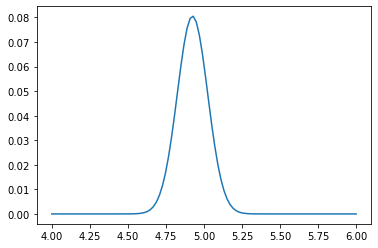
\includegraphics{Figure-12-01}
\end{figure}


\begin{python}
# Alternatively, use the analytic solution, \mathcal{L}_{n}(\mu) \sim N(\mu_hat, \sigma^{2}/n)
L_i2 = norm.pdf(mu_values, loc=mu_hat, scale=sigma/np.sqrt(n))
plt.plot(mu_values, L_i2 / L_i2.sum())
\end{python}

\begin{figure}[H]
\centering
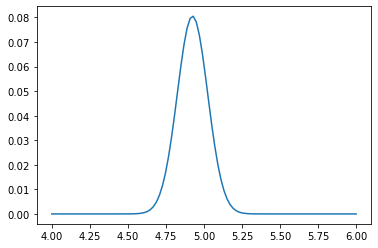
\includegraphics{Figure-12-02}
\end{figure}

\textbf{(c)}

\begin{python}
fig, (ax1,ax2) = plt.subplots(2, 1, sharex='col')
ax1.plot(mu_values, L_i2 / L_i2.sum())
posterior_samples = norm.rvs(loc=mu_hat, scale=sigma/np.sqrt(n), size=1000)
ax2.hist(posterior_samples, density=True, bins=mu_values)
\end{python}

\begin{figure}[H]
\centering
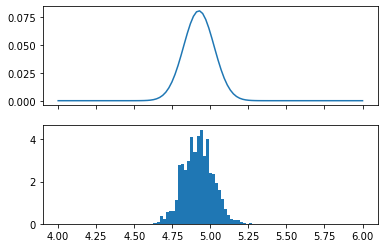
\includegraphics{Figure-12-03}
\end{figure}

\textbf{(d)}
Let \(Y = e^X\). Analytically:
\begin{itemize}[tightlist]
\item
  The CDF is
  \(F_Y(z) = \PROB_\theta(e^X \leq z) = \PROB_\mu(X \leq \log z) = \PROB_\mu \left( \frac{X - \mu}{\sigma} \leq \frac{\log z - \mu}{\sigma} \right) = \PROB(Z \leq \log z - \mu) = \Phi(\log z - \mu)\),
  where \(\Phi\) is the CDF of a standard normal distribution.
\item
  The PDF is
  \(f_Y(z) = F'_Y(z) = \partial \Phi(\log z - \mu) / \partial z = \phi(\log z - \mu) / z\),
  where \(\phi = \Phi'\) is the PDF of a standard normal function.
\end{itemize}

\begin{python}
def posterior_density(z):
    # Suppress warnings about log(z) when z < 0 and division by zero 
    # np.where will filter out invalid values
    with np.errstate(divide='ignore', invalid='ignore'):
        return np.where(z > 0, norm.pdf(np.log(z) - mu_hat) / z, 0)
    
z_values = np.linspace(0, 500, 100)
f_values = posterior_density(z_values)
plt.plot(z_values, f_values)
\end{python}

\begin{figure}[H]
\centering
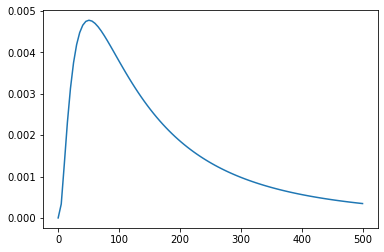
\includegraphics{Figure-12-04}
\end{figure}


\begin{python}
# By simulation:
# Resample from the estimated parametric distribution for X, and calculate Y = exp(X)
Y = np.exp(norm.rvs(loc=mu_hat, scale=sigma, size=10000))
# Recompute ranges for plot based on observed Y values
z_values = np.linspace(0, max(Y), 100)
f_values = posterior_density(z_values)
fig, (ax1,ax2) = plt.subplots(2, 1, sharex='col')
ax1.plot(z_values, f_values)
ax2.hist(Y, density=True, bins=z_values)
\end{python}

\begin{figure}[H]
\centering
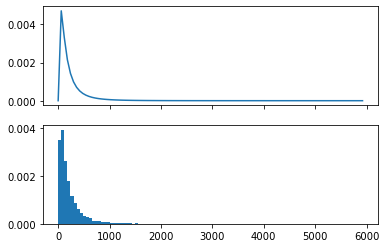
\includegraphics{Figure-12-05}
\end{figure}

\textbf{(e)}
Analytic solution: \(Y = g(X) = e^X\) and \(X \sim N(\mu, 1)\). Since
\(g\) is a monotonically increasing function, the quantiles of \(Y\) are
the exponentials of the quantiles of \(X\); that is,
\[
F_Y^{-1}(q) = g(F_X^{-1}(q)) = e^{F_X^{-1}(q)}
\]
But \(X\) follows a Normal distribution -- we can plug in the MLE for
\(\mu\), \(\hat{\mu} = \bar{X}\), obtain the quantiles for \(X\),
and then obtain the quantiles for \(Y\).
\begin{align*}
F_X^{-1}(q) &= \Phi^{-1}(q) / \sigma + \mu \\
F_Y^{-1}(q) &= e^{\Phi^{-1}(q) / \sigma + \mu}
\end{align*}

\begin{python}
from scipy.stats import norm
z_025 = norm.ppf(0.025)
z_975 = norm.ppf(0.975)
posterior_interval_analytic = (np.exp(z_025 + mu_hat), np.exp(z_975 + mu_hat))
print("95%% posterior interval (analytic):  %.3f, %.3f" % posterior_interval_analytic)
\end{python}
\begin{console}
95\% posterior interval (analytic):  19.388, 977.081
\end{console}
Alternatively, we can just sample from our simulation draws to get an
approximation:

\begin{python}
# Find percentile from simulated draws
posterior_interval_simulation = (
    np.quantile(Y, 0.025),
    np.quantile(Y, 0.975)
)
print("95%% posterior interval (simulation):  %.3f, %.3f" % posterior_interval_simulation)
\end{python}
\begin{console}
95\% posterior interval (simulation):  19.021, 985.730
\end{console}
\textbf{(f)}
For the Bayesian interval estimate, we need to find \(C = (a, b)\) such
that
\[
\int_{-\infty}^{a} f_Y(\theta | X^{n}) d\theta = \int_b^{\infty} f_Y(\theta | X^{n}) d\theta = \frac{\alpha}{2}
\]
or, using the cumulative density functions,
\[
F_Y(a) = 1 - F_Y(b) = \frac{\alpha}{2}
\]
\[
\Phi(\log a - \mu) = 1 - \Phi(\log b - \mu) = \frac{\alpha}{2}
\]
Solving for \(a\) and \(b\),
\[
a = e^{\mu + \Phi^{-1}(\alpha / 2)}
\quad \text{and} \quad
b = e^{\mu + \Phi^{-1}(1 - \alpha / 2)}
\]
This is exactly the same calculation as the analytic solution for the
posterior interval.

\begin{python}
from scipy.stats import norm
z_025 = norm.ppf(0.025)
z_975 = norm.ppf(0.975)
confidence_interval_analytic = (np.exp(z_025 + mu_hat), np.exp(z_975 + mu_hat))
print("95%% confidence interval (analytic):  %.3f, %.3f" % confidence_interval_analytic)
\end{python}
\begin{console}
95\% confidence interval (analytic):  19.388, 977.081
\end{console}

\textbf{Exercise 12.11.3}. Let
\(X_{1}, \dots, X_{n} \sim \text{Uniform}(0, \theta)\). Let
\(f(\theta) \propto 1/\theta\). Find the posterior density.

\textbf{Solution}. The posterior density is proportional to the
likelihood times the prior:
\begin{align*}
f(\theta | X^{n}) &\propto \mathcal{L}_{n}(\theta) f(\theta) \\
&= \frac{1}{\theta} \prod_{i=1}^{n} f(X_{i}; \theta)  \\
&= \frac{1}{\theta} \prod_{i=1}^{n} \frac{I(X_{i} \leq \theta)}{\theta} \\
&= \theta^{-(n+1)} I( \max \{ X_{1}, \dots, X_{n} \} \leq \theta \} ) \\
&= \begin{cases}
\theta^{-(n+1)} & \text{if } \theta \geq \max \{ X_{1}, \dots, X_{n} \} \\
0 & \text{otherwise}
\end{cases}
\end{align*}
Now we just need to normalize the posterior density so it integrates to
1. Let \(m = \max \{ X_{1}, \dots, X_{n} \}\). Then:
\[
1 = \int_{-\infty}^{\infty} f(\theta) d\theta  = \int_m^{\infty} c \theta^{-(n+1)} d\theta = c m^{-n} / n
\]
Solving this we get \(c = n m^{n}\), so the posterior density is:
\[
f(\theta) = \begin{cases}
\frac{n}{\theta} \left(\frac{m}{\theta}\right)^{n} & \text{if } \theta \geq m \\
0 & \text{otherwise}
\end{cases}
\]
where \(m = \max \{ X_{1}, \dots, X_{n} \}\).

\textbf{Exercise 12.11.4}. Suppose that 50 people are given a placebo
and 50 are given a new treatment. 30 placebo patients show improvement
while 40 treated patients show improvement. Let \(\tau = p_{2} - p_{1}\)
where \(p_{2}\) is the probability of improving under treatment and
\(p_{1}\) is the probability of improving under placebo.
\textbf{(a)} Find the MLE of \(\tau\). Find the standard error and 90\%
confidence interval using the delta method.
\textbf{(b)} Find the standard error and 90\% confidence interval using
the parametric bootstrap.
\textbf{(c)} Use the prior \(f(p_{1}, p_{2}) = 1\). Use simulation to find
the posterior mean and posterior 90\% interval for \(\tau\).
\textbf{(d)} Let
\[
\psi = \log \left( \left( \frac{p_{1}}{1 - p_{1}} \div \frac{p2}{1 - p2} \right) \right)
\]
be the log-odds ratio. Note that \(\psi = 0\) if \(p_{1} = p_{2}\). Find the
MLE of \(\psi\). Use the delta method to find a 90\% confidence interval
for \(\psi\).
\textbf{(e)} Use simulation to find the posterior mean and posterior
90\% interval for \(\psi\).

\textbf{Solution}.
\textbf{(a)}
We have two random variables, \(X_{1} \sim \text{Binomial}(n_{1}, p_{1})\) and
\(X_{2} \sim \text{Binomial}(n_{2}, p_{2})\). We are given \(n_{1} = n_{2} = 50\),
and the measurements \(X_{1} = 30\) and \(X_{2} = 40\).
We wish to estimate \(\tau = g(p_{1}, p_{2}) = p_{2} - p_{1}\). The MLE is
simply
\(\hat{\tau} = g(\hat{p}_{1}, \hat{p}_{2}) = \hat{p}_{2} - \hat{p}_{1} = X_{2} / n_{2} - X_{1} / n_{1}\).
Using the multiparameter delta method, the gradient of \(g\) is
\[
\nabla g = 
\begin{pmatrix} \partial g / \partial p_{1} \\ \partial g / \partial p_{2} \end{pmatrix} 
= \begin{pmatrix} -1 \\ 1 \end{pmatrix} 
\]
The log likelihood is:
\begin{align*}
\ell(p_{1}, p_{2}) &= \log f_{X_{1}}(X_{1}; p_{1}) + \log f_{X_{2}}(X_{2}; p_{2}) \\
& = \log \binom{n_{1}}{X_{1}} p_{1}^{X_{1}} (1 - p_{1})^{n_{1} - X_{1}}
+ \log \binom{n_{2}}{X_{2}} p_{2}^{X_{2}} (1 - p_{2})^{n_{2} - X_{2}} \\
&= \log \binom{n_{1}}{X_{1}} + X_{1} \log p_{1} + (n_{1} - X_{1}) \log (1 - p_{1})
\\
& \quad 
+ \log \binom{n_{2}}{X_{2}} + X_{2} \log p_{2} + (n_{2} - X_{2}) \log (1 - p_{2}) \\
&= X_{1} \log p_{1} + (n_{1} - X_{1}) \log (1 - p_{1}) + X_{2} \log p_{2} + (n_{2} - X_{2}) \log (1 - p_{2}) + C
\end{align*}
where \(C\) does not depend on \(p_{1}\) or \(p_{2}\).
The partial derivatives of the log likelihood are:
\begin{align*}
\Frac{\partial^{2} \ell}{\partial p_{1}^{2}} & = - \Frac{X_{1}}{p_{1}^{2}} - \frac{n_{1} - X_{1}}{(1 - p_{1})^{2}} \\
\Frac{\partial^{2} \ell}{\partial p_{2}^{2}} & = - \Frac{X_{2}}{p_{2}^{2}} - \frac{n_{2} - X_{2}}{(1 - p_{2})^{2}} \\
\Frac{\partial^{2} \ell}{\partial p_{1} \partial p_{2}} & = 0
\end{align*}
The Fisher Information Matrix is
\[
I_{n}(p_{1}, p_{2}) = -\begin{pmatrix}
\EXP\left[ \Frac{\partial^{2} \ell}{\partial p_{1}^{2}} \right]
& \EXP\left[ \Frac{\partial^{2} \ell}{\partial p_{1} \partial p_{2}} \right]  \\
\EXP\left[ \Frac{\partial^{2} \ell}{\partial p_{1} \partial p_{2}} \right]
& \EXP\left[ \Frac{\partial^{2} \ell}{\partial p_{2}^{2}} \right]
\end{pmatrix} = \begin{pmatrix}
\Frac{n_{1}}{p_{1}(1 - p_{1})} & 0 \\
0 & \Frac{n_{2}}{p_{2}(1 - p_{2})}
\end{pmatrix}
\]
and its inverse is
\[
J_{n}(p_{1}, p_{2}) = I_{n}^{-1}(p_{1}, p_{2}) = 
\begin{pmatrix} 
\Frac{p_{1}(1 - p_{1})}{n_{1}} & 0 \\
0 & \Frac{p_{2}(1 - p_{2})}{n_{2}}
\end{pmatrix}
\]
Then,
\[
\widehat{\SE}(\hat{\tau}) = \sqrt{(\hat{\nabla}g)^T \hat{J}_{n} (\hat{\nabla}g)}
= \sqrt{\frac{\hat{p}_{1}(1 - \hat{p}_{1})}{n_{1}} + \frac{\hat{p}_{2}(1 - \hat{p}_{2})}{n_{2}}}
\]
And we get the confidence interval:
\[
\hat{\tau} \pm z_{1 - \alpha/2}\widehat{\SE}(\hat{\tau})
\]

\begin{python}
import numpy as np
from scipy.stats import norm
n1 = 50
n2 = 50
X1 = 30
X2 = 40
p1_hat = X1 / n1
p2_hat = X2 / n2
tau_hat = p2_hat - p1_hat
se_hat = np.sqrt((p1_hat * (1 - p1_hat) / n1) + (p2_hat * (1 - p2_hat) / n2))
z_90 = norm.ppf(0.95)
confidence_interval = (tau_hat - z_90 * se_hat, tau_hat + z_90 * se_hat)
print('Estimated difference of means: \t\t %.3f' % tau_hat)
print('Estimated 90%% confidence interval:\t %.3f, %.3f' % confidence_interval)
\end{python}
\begin{console}
Estimated difference of means:           0.200
Estimated 90\% confidence interval:       0.053, 0.347
\end{console}
\textbf{(b)}

\begin{python}
import numpy as np
from scipy.stats import binom
B = 100000
n1 = 50
n2 = 50
X1 = 30
X2 = 40
p1_hat = X1 / n1
p2_hat = X2 / n2
XX1 = binom.rvs(n1, p1_hat, size=B)
XX2 = binom.rvs(n2, p2_hat, size=B)
tau_boot = XX2 / n2 - XX1 / n1
tau_boot_hat = tau_boot.mean()
q_05 = np.quantile(tau_boot, 0.05)
q_95 = np.quantile(tau_boot, 0.95)
boot_confidence_interval = (q_05, q_95)
print('Estimated difference of means: \t\t %.3f' % tau_boot_hat)
print('Estimated 90%% confidence interval:\t %.3f, %.3f' % boot_confidence_interval)
\end{python}
\begin{console}
Estimated difference of means:           0.200
Estimated 90\% confidence interval:       0.060, 0.340
\end{console}
\textbf{(c)} The posterior density is proportional to the likelihood
times the prior:
\begin{align*}
f((p_{1}, p_{2}) | X^{2}) &\propto \mathcal{L}(p_{1}, p_{2} | X^{2}) f(p_{1}, p_{2}) \\
&= f_{X_{1}}(X_{1} | p_{1}) f_{X_{2}}(X_{2} | p_{1}) \cdot 1 \\
&= \binom{n_{1}}{X_{1}} p_{1}^{X_{1}} (1 - p_{1})^{n_{1} - X_{1}} \binom{n_{2}}{X_{2}} p_{2}^{X_{2}} (1 - p_{2})^{n_{2} - X_{2}} \\
&\propto p_{1}^{X_{1}} (1 - p_{1})^{n_{1} - X_{1}} p_{2}^{X_{2}} (1 - p_{2})^{n_{2} - X_{2}} \\
&\propto f(p_{1} | X_{1}) f(p_{2} | X_{2})
\end{align*}
where
\[
p_{1} | X_{1} \sim \text{Beta}(X_{1} + 1, n_{1} - X_{1} + 1) 
\quad \text{and} \quad
p_{2} | X_{2} \sim \text{Beta}(X_{2} + 1, n_{2} - X_{2} + 1)
\]
We can now sample from the Beta distributions to sample \(p_{1}\),
\(p_{2}\), and for each pair of samples, compute the sample
\(\tau = p_{2} - p_{1}\).

\begin{python}
from scipy.stats import beta
B = 100000
n1 = 50
n2 = 50
X1 = 30
X2 = 40
p1_boot = beta.rvs(X1 + 1, n1 - X1 + 1, size=B)
p2_boot = beta.rvs(X2 + 1, n2 - X2 + 1, size=B)
tau_boot = p2_boot - p1_boot
tau_boot_hat = tau_boot.mean()
q_05 = np.quantile(tau_boot, 0.05)
q_95 = np.quantile(tau_boot, 0.95)
boot_confidence_interval = (q_05, q_95)
print('Estimated posterior mean: \t\t %.3f' % tau_boot_hat)
print('Estimated 90%% confidence interval:\t %.3f, %.3f' % boot_confidence_interval)
\end{python}
\begin{console}
Estimated posterior mean:                0.193
Estimated 90\% confidence interval:       0.047, 0.335
\end{console}
\textbf{(d)}
Let
\(\psi = h(p_{1}, p_{2}) = \log p_{1} - \log (1 - p_{1}) - \log p_{2} + \log (1 - p_{2})\).
The MLE is just \(\hat{\psi} = h(\hat{p}_{1}, \hat{p}_{2})\).
Using the multiparameter delta method, the gradient of \(h\) is:
\[
\nabla h = 
\begin{pmatrix}
\frac{\partial h}{\partial p_{1}} \\ 
\frac{\partial h}{\partial p_{2}} \end{pmatrix}
= \begin{pmatrix}
\frac{1}{p_{1}(1 - p_{1})} \\
-\frac{1}{p_{2}(1 - p_{2})}
\end{pmatrix}
\]
The inverse Fisher Information Matrix is still:
\[
J_{n}(p_{1}, p_{2}) = \begin{pmatrix}
\frac{p_{1}(1 - p_{1})}{n_{1}} & 0 \\
0 & \frac{p_{2}(1 - p_{2})}{n_{2}}
\end{pmatrix}
\]
and so the estimated standard error is:
\begin{align*}
\widehat{\SE}(\hat{\psi}) &= \sqrt{(\hat{\nabla}h)^T \hat{J}_{n} (\hat{\nabla}h)} \\
&= 
\sqrt{\begin{pmatrix}
\frac{1}{\hat{p}_{1}(1 - \hat{p}_{1})} &
-\frac{1}{\hat{p}_{2}(1 - \hat{p}_{2})}
\end{pmatrix}
\begin{pmatrix}
\frac{\hat{p}_{1}(1 - \hat{p}_{1})}{n_{1}} & 0 \\
0 & \frac{\hat{p}_{2}(1 - \hat{p}_{2})}{n_{2}}
\end{pmatrix}
\begin{pmatrix}
\frac{1}{\hat{p}_{1}(1 - \hat{p}_{1})} \\
-\frac{1}{\hat{p}_{2}(1 - \hat{p}_{2})}
\end{pmatrix}} \\
&= \sqrt{\frac{1}{n_{1} \hat{p}_{1}(1 - \hat{p}_{1})} + \frac{1}{n_{2} \hat{p}_{2}(1 - \hat{p}_{2})}}
\end{align*}
and we get the confidence interval:
\[
\hat{\psi} \pm z_{1 - \alpha/2} \widehat{\SE}(\hat{\psi})
\]

\begin{python}
import numpy as np
from scipy.stats import norm
n1 = 50
n2 = 50
X1 = 30
X2 = 40
p1_hat = X1 / n1
p2_hat = X2 / n2
psi_hat = np.log((p1_hat / (1 - p1_hat)) / (p2_hat / (1 - p2_hat)))
se_hat = np.sqrt(1/(n1 * p1_hat * (1 - p1_hat)) + 1/(n2 * p2_hat * (1 - p2_hat)))
z_90 = norm.ppf(0.95)
confidence_interval = (psi_hat - z_90 * se_hat, psi_hat + z_90 * se_hat)
print('Estimated log-odds ratio: \t\t %.3f' % psi_hat)
print('Estimated 90%% confidence interval:\t %.3f, %.3f' % confidence_interval)
\end{python}
\begin{console}
Estimated log-odds ratio:                -0.981
Estimated 90\% confidence interval:       -1.732, -0.230
\end{console}
\textbf{(e)} The probability distributions for \(p_{1} | X_{1}\) and
\(p_{2} | X_{2}\) are still the same -- we are just computing
\(\psi = h(p_{1}, p_{2})\) for each simulation sample now, rather than
\(\tau = g(p_{1}, p_{2})\).

\begin{python}
from scipy.stats import beta
B = 100000
n1 = 50
n2 = 50
X1 = 30
X2 = 40
p1_boot = beta.rvs(X1 + 1, n1 - X1 + 1, size=B)
p2_boot = beta.rvs(X2 + 1, n2 - X2 + 1, size=B)
psi_boot = np.log((p1_boot / (1 - p1_boot)) / (p2_boot / (1 - p2_boot)))
psi_boot_hat = psi_boot.mean()
q_05 = np.quantile(psi_boot, 0.05)
q_95 = np.quantile(psi_boot, 0.95)
boot_confidence_interval = (q_05, q_95)
print('Estimated posterior mean: \t\t %.3f' % psi_boot_hat)
print('Estimated 90%% confidence interval:\t %.3f, %.3f' % boot_confidence_interval)
\end{python}
\begin{console}
Estimated posterior mean:                -0.953
Estimated 90\% confidence interval:       -1.699, -0.224
\end{console}

\textbf{Exercise 12.11.5}. Consider the \(\text{Bernoulli}(p)\)
observations
\[
0\; 1\; 0\; 1\; 0\; 0\; 0\; 0\; 0\; 0
\]
Plot the posterior for \(p\) using these priors:
\(\text{Beta}(1/2, 1/2)\), \(\text{Beta}(1, 1)\),
\(\text{Beta}(10, 10)\), \(\text{Beta}(100, 100)\).

\textbf{Solution}.
The observations include \(n = 10\) samples, of which \(k = 2\) samples
with observed value 1. Assume a prior of the form
\(\text{Beta}(\alpha, \beta)\).
The posterior is proportional to the likelihood times the prior.
\begin{align*}
f(p | X^{n}) & \propto \mathcal{L}(p | x^{n}) f(p) \\
&= \binom{n}{k} p^{k} (1 - p)^{n-k} \frac{p^{\alpha - 1}(1-p)^{\beta - 1}}{B(\alpha, \beta)}\\
&\propto p^{k + \alpha - 1} (1 - p)^{n - k + \beta - 1}
\end{align*}
This density is proportional to a Beta density function in p, so
\[
p | X^{n} \sim \text{Beta}(k + \alpha - 1, n - k + \beta - 1)
\]
Now, plotting the posterior becomes just a matter of plotting these beta
distributions.
When \(\alpha\) and \(\beta\) are integers, we can also reinterpret this
posterior as equivalent to starting with a flat prior and observing
extra \(\alpha + \beta\) events, with \(\alpha\) extra events producing
outcome 1 and \(\beta\) extra events producing outcome 0. This is shown
on the plots below -- the larger the number of ``extra observations'',
the less impact the actual observations make on shifting the belief
about the true parameter value.

\begin{python}
import numpy as np
from scipy.stats import beta
import matplotlib.pyplot as plt
n = 10
k = 2
x = np.linspace(0, 1, 200)
plt.figure(figsize=(12, 8))
for a, b in [(1/2, 1/2), (1, 1), (10, 10), (100, 100)]:
    plt.plot(x, beta.pdf(x, k + a - 1, n - k + b - 1), 
             label='prior = Beta(' + str(a) + ', ' + str(b) +')')
    plt.legend()
plt.show()
\end{python}

\begin{figure}[H]
\centering
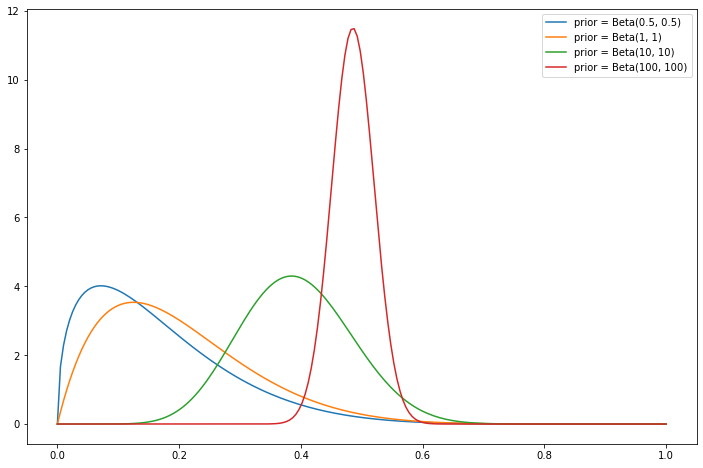
\includegraphics{Figure-12-06}
\end{figure}

    

\textbf{Exercise 12.11.6}. Let
\(X_{1}, \dots, X_{n} \sim \text{Poisson}(\lambda)\).
\textbf{(a)} Let \(\lambda \sim \text{Gamma}(\alpha, \beta)\) be the
prior. Show that the posterior is also a Gamma. Find the posterior mean.
\textbf{(b)} Find the Jeffreys' prior. Find the posterior.

\textbf{Solution}.
\textbf{(a)} The posterior is proportional to the likelihood times the
prior:
\begin{align*}
f(\lambda | X^{n}) &\propto \mathcal{L}(\lambda | X^{n}) f(\lambda) \\
&= \left(\prod_{i=1}^{n} \frac{\lambda^{X_{i}}e^{-\lambda}}{X_{i}!} \right) \frac{\beta^{\alpha}}{\Gamma(\alpha)}\lambda^{\alpha - 1}e^{-\beta \lambda} \\
& \propto \lambda^{\sum_{i} X_{i}} e^{-n\lambda} \lambda^{\alpha - 1}e^{-\beta \lambda} \\
&= \lambda^{\left(\alpha + \sum_{i} X_{i} \right) - 1} e^{-(\beta + n) \lambda}
\end{align*}
Therefore, the posterior is proportional to a Gamma distribution with
parameters \(\left(\alpha + \sum_{i=1}^{n} X_{i}, \beta + n\right)\) -- and
thus it must be drawn from that distribution.
\[
\lambda | X^{n} \sim \text{Gamma}\left(\alpha + \sum_{i=1}^{n} X_{i}, \beta + n \right)
\]
The posterior mean is the mean of Gamma distribution it is drawn from,
\[
\bar{\lambda} | X^{n} = \frac{\alpha + \sum_{i=1}^{n} X_{i}}{\beta + n}
\]
\textbf{(b)} For a Poisson distribution, the log likelihood is
\begin{align*}
\ell_{n}(\lambda) &= \sum_{i=1}^{n} \log \left( \frac{\lambda^{X_{i}} e^{-\lambda}}{X_{i}!}\right)  \\
&= \sum_{i=1}^{n} \left( X_{i} \log \lambda - \lambda - \log (X_{i}!)\right) \\
&= \log \lambda \left( \sum_{i=1}^{n} X_{i} \right) - n\lambda - \sum_{i=1}^{n} \log (X_{i}!)
\end{align*}
Its second derivative is
\(\ell_{n}''(\lambda) = -n \bar{X} / \lambda^{2}\), so Fisher's
information is
\(I(\lambda) = -\EXP[\ell''(\lambda)] = 1 / \lambda\).
Jeffreys' prior is:
\[
f(\lambda) \propto I(\lambda)^{1/2} = \lambda^{-1/2}
\]
The posterior is proportional to the likelihood times the prior:
\begin{align*}
f(\lambda | X^{n}) &\propto \mathcal{L}(\lambda | X^{n}) f(\lambda) \\
&\propto \left(\prod_{i=1}^{n} \frac{\lambda^{X_{i}}e^{-\lambda}}{X_{i}!} \right) \lambda^{-1/2} \\
&\propto \lambda^{\left(1/2 + \sum_{i} X_{i} \right) - 1} e^{-n\lambda}
\end{align*}
Therefore, the posterior is proportional to a Gamma distribution with
parameters \(\left(\left(1/2 + \sum_{i=1}^{n} X_{i} \right), n\right)\) --
and thus it must be drawn from that distribution.
\[
\lambda | X^{n} \sim \text{Gamma}\left(\frac{1}{2} + \sum_{i=1}^{n} X_{i}, n \right)
\]


% Chapter 13
\section*{13. Statistical Decision Theory}\label{statistical-decision-theory}

\subsection*{13.1 Preliminaries}\label{preliminaries}
\textbf{Decision theory} is a formal theory for comparing between
statistical procedures.
In the language of decision theory, a estimator is sometimes called a
\textbf{decision rule} and the possible values of the decision rule are
called \textbf{actions}.
We shall measure the discrepancy between \(\theta\) and \(\hat{\theta}\)
using a \textbf{loss function} \(L(\theta, \hat{\theta})\). Formally,
\(L\) maps \(\Theta \times \Theta\) into \(\R\).
The \textbf{risk} of an estimator \(\hat{\theta}\) is
\[
R(\theta, \hat{\theta}) = \EXP_{\theta} \left( L(\theta, \hat{\theta}) \right)
= \int L(\theta, \hat{\theta}(x)) f(x; \theta) dx
\]
When the loss function is squared error, then the risk is just the mean
squared error:
\[
R(\theta, \hat{\theta}) = \EXP_{\theta}(\hat{\theta} - \theta)^{2} = \MSE = \VAR_\theta(\hat{\theta}) + \text{bias}_\theta^{2}(\hat{\theta})
\]
In the rest of chapter, if the risk function is not specified, assume
the loss function is the squared error.

\subsection*{13.2 Comparing Risk
Functions}\label{comparing-risk-functions}
The \textbf{maximum risk} is
\[
\bar{R}(\hat{\theta}) = \sup_\theta R(\theta, \hat{\theta})
\]
and the \textbf{Bayes risk} is
\[
r(\pi, \hat{\theta}) = \int R(\theta, \hat{\theta}) \pi(\theta) d\theta
\]
where \(\pi(\theta)\) is a prior for \(\theta\).
An estimator that minimizes the maximum risk is called a \textbf{minimax
rule}. Formally, \(\hat{\theta}\) is minimax if
\[
R(\theta, \hat{\theta}) = \inf_{\bar{\theta}} \sup_\theta R(\theta, \hat{\theta})
\]
where the infimum is over all estimators \(\bar{\theta}\).
A decision rule that minimizes the Bayes risk is called a \textbf{Bayes
rule}. Formally, \(\hat{\theta}\) is a Bayes rule for prior \(\pi\) if
\[
R(\theta, \hat{\theta}) = \inf_{\bar{\theta}} r(\pi, \bar{\theta})
\]
where the infimum is over all estimators \(\bar{\theta}\).

\subsection*{13.3 Bayes Estimators}\label{bayes-estimators}
Let \(\pi\) be a prior. From Bayes' Theorem, the posterior density is
\[
f(\theta | x) = \frac{f(x | \theta) \pi(\theta)}{m(x)} = \frac{f(x | \theta) \pi(\theta)}{\int f(x | \theta) \pi(\theta) d\theta}
\]
where
\(m(x) = \int f(x, \theta) d\theta = \int f(x | \theta) \pi(\theta) d\theta\)
is the \textbf{marginal distribution} of \(X\). Define the
\textbf{posterior risk} of an estimator \(\hat{\theta}(x)\) by
\[
r(\hat{\theta} | x) = \int L(\theta, \hat{\theta}(x)) f(\theta | x) d\theta
\]

\textbf{Theorem 13.8}. The Bayes risk \(r(\pi, \hat{\theta})\) satisfies
\[
r(\pi, \hat{\theta}) = \int r(\hat{\theta} | x) m(x) dx
\]
Let \(\hat{\theta}(x)\) be the value of \(\theta\) that minimizes
\(r(\hat{\theta} | x)\). Then \(\hat{\theta}\) is the Bayes estimator.
\textbf{Proof}. We can rewrite the Bayes risk as:
\begin{align*}
r(\pi, \hat{\theta} &= \int R(\theta, \hat{\theta}) \pi(\theta) d\theta = \int \left( \int L(\theta, \hat{\theta}(x)) f(x | \theta) dx \right) \pi(\theta) d\theta \\
&= \int \int L(\theta, \hat{\theta}(x)) f(x, \theta) dx d\theta = \int \int L(\theta, \hat{\theta}(x)) f(\theta | x) m(x) dx d\theta \\
&= \int \left(\int L(\theta, \hat{\theta}(x) d\theta \right) m(x) dx = \int r(\hat{\theta} | x) m(x) dx
\end{align*}
If \(\hat{\theta} = \text{argmin}_\theta r(\hat{\theta} | x)\) then we
will minimize the integrand at every \(x\) and thus minimize the
integral \(\int r(\hat{\theta} | x)m(x) dx\).

\textbf{Theorem 13.9}. If
\(L(\theta, \hat{\theta}) = (\theta - \hat{\theta})^{2}\) then the Bayes
estimator is
\[
\hat{\theta}(x) = \int \theta f(\theta | x) d\theta = \EXP(\theta | X = x)
\]
If \(L(\theta, \hat{\theta}) = |\theta - \hat{\theta}|\) then the Bayes
estimator is the median of the posterior \(f(\theta | x)\). If
\(L(\theta, \hat{\theta})\) is zero-one loss, then the Bayes estimator
is the mode of the posterior \(f(\theta | x)\).
\textbf{Proof}. We will prove the Theorem for the squared error loss.
The Bayes rule \(\hat{\theta}\) minimizes
\(r(\theta | x) = \int (\theta - \hat{\theta}(x))^{2} f(\theta | x) d\theta\).
Taking the derivative of \(r(\hat{\theta} | x)\) with respect to
\(\hat{\theta}(x)\) and setting it to 0 yields the equation
\(2 \int (\theta - \hat{\theta}(x)) f(\theta | x) d\theta = 0\). Solving
for \(\hat{\theta}(x)\) we get the given estimator.

\subsection*{13.4 Minimax Rules}\label{minimax-rules}
The problem of Minimax Rules is complicated and a complete coverage of
that theory will not be attempted here, but a few key results will be
mentioned. Main takeaway message from this section: Bayes estimators
with a constant risk function are minimax.

\textbf{Theorem 13.11}. Let \(\hat{\theta}^\pi\) be the Bayes rule for
some prior \(\pi\):
\[
r(\pi, \hat{\theta}^\pi) = \inf_{\hat{\theta}} r(\pi, \hat{\theta})
\]
Suppose that
\[
R(\theta, \hat{\theta}^\pi) \leq r(\pi, \hat{\theta}^\pi) \;\text{for all } \theta
\]
Then \(\hat{\theta}^\pi\) is minimax and \(\pi\) is called a
\textbf{least favorable prior}.
\textbf{Proof}. Suppose that \(\hat{\theta}^\pi\) is not minimax. Then
there is another rule \(\hat{\theta}_{0}\) such that
\(\sup_\theta R(\theta, \hat{\theta}_{0}) \leq \sup_\theta R(\theta, \hat{\theta}^\pi)\).
Since the average of a function is always less than or equal to its
maximum, we have that
\(r(\theta, \hat{\theta}_{0}) \leq \sup_\theta R(\theta, \hat{\theta}_{0})\).
Hence,
\[
r(\theta, \hat{\theta}_{0}) \leq \sup_\theta R(\theta, \hat{\theta}_{0}) \leq \sup_\theta R(\theta, \hat{\theta}^\pi) \leq r(\pi, \hat{\theta}^\pi)
\]
which contradicts
\(r(\pi, \hat{\theta}^pi) = \inf_{\hat{\theta}} r(\pi, \hat{\theta})\).

\textbf{Theorem 13.12}. Suppose that \(\hat{\theta}\) is the Bayes rule
estimator with respect to some prior \(\pi\). Suppose further that
\(\hat{\theta}\) has constant risk: \(R(\theta, \hat{\theta}) = c\) for
some \(c\). Then \(\hat{\theta}\) is minimax.
\textbf{Proof}. The Bayes risk is
\(r(\pi, \hat{\theta}) = \int R(\theta, \hat{\theta}) \pi(\theta) d\theta = c\)
and hence \(R(\theta, \hat{\theta}) \leq r(\pi, \hat{\theta})\) for all
\(\theta\). Now apply Theorem 13.11.

\textbf{Theorem 13.15}. Let \(X_{1}, \dots, X_{n} \sim N(\theta, 1)\) and
let \(\hat{\theta} = \bar{X}\). Then \(\hat{\theta}\) is minimax
with respect to any well-behaved loss function. It is the only estimator
with this property.
\emph{Well-behaved means that the level sets must be convex and
symmetric about the origin. The result holds up to sets of measure 0.}

\subsection*{13.5 Maximum Likelihood, Minimax and
Bayes}\label{maximum-likelihood-minimax-and-bayes}
For parametric models that satisfy weak regularity conditions, the MLE
is approximately minimax. Consider squared error loss which is squared
bias plus variance. In parametric models with large samples, it can be
shown that the variance term dominates the bias so the risk of the MLE
\(\hat{\theta}\) roughly equals the variance:
\[
R(\theta, \hat{\theta}) = \VAR_\theta(\hat{\theta}) + \text{bias}^{2} \approx \VAR_\theta(\hat{\theta})
\]
\emph{Typically, the squared bias is of order \(O(n^{-2})\) while the
variance is of order \(O(n^{-1})\).}
As seen on the chapter on parametric models, the variance is
approximately:
\[
\VAR(\hat{\theta}) = \frac{1}{nI(\theta)}
\]
where \(I(\theta)\) is the Fisher information. Hence,
\[
n R(\theta, \hat{\theta}) \approx \frac{1}{I(\theta)}
\]
For any other estimator \(\theta'\), it can be shown that, for large
\(n\), \(R(\theta, \theta') \geq R(\theta, \hat{\theta})\). More
precisely,
\[
\lim_{\epsilon \rightarrow 0} \limsup_{n \rightarrow \infty} \sup_{|\theta - \theta'| < \epsilon} n R(\theta', \hat{\theta}) \geq \frac{1}{I(\theta)}
\]
This says that, in a local, large sample sense, the MLE is minimax. It
can also be shown that the MLE is approximately the Bayes rule.
In summary, in parametric models with large samples, the MLE is
approximately minimax and Bayes. There is a caveat: these results break
down when the number of parameters is large.

\subsection*{13.6 Admissibility}\label{admissibility}
An estimator \(\hat{\theta}\) is \textbf{inadmissible} if there exists
another rule \(\hat{\theta}'\) such that
\begin{align*}
R(\theta, \hat{\theta}') \leq R(\theta, \hat{\theta}) & \quad \text{for all } \theta \text{ and} \\
R(\theta, \hat{\theta}') < R(\theta, \hat{\theta}) & \quad \text{for at least one } \theta
\end{align*}
A prior has \textbf{full support} if for every \(\theta\) and every
\(\epsilon > 0\),
\(\int_{\theta - \epsilon}^{\theta + \epsilon} \pi(\theta) d\theta > 0\).

\textbf{Theorem 13.20 (Bayes' rules are admissible)}. Suppose that
\(\theta \subset \R\) and that \(R(\theta, \hat{\theta})\) is a
continuous function of \(\theta\) for every \(\hat{\theta}\). Let
\(\pi\) be a prior density with full support and let
\(\hat{\theta}^\pi\) be the Bayes' rule. If the Bayes risk is finite
then \(\hat{\theta}^\pi\) is admissible.
\textbf{Proof}. Suppose \(\hat{\theta}^\pi\) is inadmissible. Then there
exists a better rule \(\hat{\theta}\) such that
\(R(\theta, \hat{\theta}) \leq R(\theta, \hat{\theta}^\pi)\) for all
\(\theta\) and
\((\theta_{0}, \hat{\theta}) < R(\theta_{0}, \hat{\theta}^\pi)\) for some
\(\theta_{0}\). Let
\(v = R(\theta_{0}, \hat{\theta}^\pi) - R(\theta_{0}, \hat{\theta}) > 0\).
Since \(R\) is continuous, there is an \(\epsilon > 0\) such that
\(R(\theta, \hat{\theta}^\pi) - R(\theta_{0}, \hat{\theta}) > v/2\) for
all \(\theta \in (\theta_{0} - \epsilon, \theta_{0} + \epsilon)\). Now,
\begin{align*}
r(\pi, \hat{\theta}^pi) - r(\pi, \hat{\theta}) &= \int R(\theta, \hat{\theta}^\pi) \pi(\theta) d\theta - \int R(\theta, \hat{\theta}) \pi(\theta) d\theta \\
&= \int \left[ R(\theta, \hat{\theta}^\pi) - R(\theta, \hat{\theta})\right] \pi(\theta) d\theta \\
&\geq \int_{\theta_{0} - \epsilon}^{\theta_{0} + \epsilon} \left[ R(\theta, \hat{\theta}^\pi) - R(\theta, \hat{\theta})\right] \pi(\theta) d\theta \\
& \geq \frac{v}{2} \int_{\theta_{0} - \epsilon}^{\theta_{0} + \epsilon} \pi(\theta) d\theta \\
& > 0
\end{align*}
Hence \(r(\pi, \hat{\theta}^\pi) > r(\pi, \hat{\theta})\). This implies
that \(\hat{\theta}^\pi\) does not minimize \(r(\pi, \hat{\theta})\),
which contradicts the fact that \(\hat{\theta}^\pi\) is the Bayes rule.

\textbf{Theorem 13.21}. Let \(X_{1}, \dots, X_{n} \sim N(\mu, \sigma^{2})\).
Under squared error loss, \(\bar{X}\) is admissible.
The proof of this Theorem is very technical and ommitted. Outline: the
posterior mean is admissible for any strictly positive prior. Take the
prior to be \(N(a, b^{2})\). When \(b^{2}\) is very large, the posterior
mean is approximately equal to \(\bar{X}\).
In general, a rule may be minimax, admissible, both, or neither. Here
are some facts linking admissibility and minimaxity.

\textbf{Theorem 13.22}. Suppose that \(\hat{\theta}\) has constant risk
and is admissible. Then it is minimax.
\textbf{Proof}. The risk is \(R(\theta, \hat{\theta}) = c\) for some
constant \(c\). If \(\hat{\theta}\) were not minimax then there exists a
rule \(\hat{\theta}'\) that further reduces the risk,
\[
R(\theta, \hat{\theta}') \leq \sup_{\theta} R(\theta, \hat{\theta}') < \sup_{\theta} R(\theta, \hat{\theta}) = c
\]
But that would imply that \(\hat{\theta}\) is inadmissible.

\textbf{Theorem 13.23}. Let \(X_{1}, \dots, X_{n} \sim N(\theta, 1)\). Then,
under squared error loss, \(\hat{\theta} = \bar{X}\) is minimax.
\textbf{Proof}. According to Theorem 13.21, \(\hat{\theta}\) is
admissible. The risk of \(\hat{\theta}\) is \(1/n\) which is constant.
According to Theorem 13.22, it is also minimax.
Although miminax rules are not guaranteed to be admissible they are
``close to admissible''. Say \(\hat{\theta}\) is \textbf{strongly
inadmissible} if there is a rule \(\hat{\theta}'\) and an
\(\epsilon > 0\) such that
\(R(\theta, \hat{\theta}') < R(\theta, \hat{\theta}) - \epsilon\) for
all \(\theta\).

\textbf{Theorem 13.24}. If \(\hat{\theta}\) is minimax then it is not
strongly inadmissible.

\subsection*{13.7 Stein's Paradox}\label{steins-paradox}
Suppose that \(X \sim N(0, 1)\) and consider estimating \(\theta\) with
squared error loss. From the previous section we know that
\(\hat{\theta}(X) = X\) is admissible.
Now consider estimating two, unrelated quantities
\(\theta = (\theta_{1}, \theta_{2})\) and suppose that
\(X_{1} \sim N(\theta_{1}, 1)\) and \(X_{2} \sim N(\theta_{2}, 1)\)
independently, with loss
\(L(\theta, \hat{\theta}) = \sum_{j=1}^{2} (\theta_{j} - \hat{\theta}_{j})^{2}\).
Not surprisingly, \(\hat{\theta}(X) = X\) is again admissible, where
\(X = (X_{1}, X_{2})\).
Now consider the generalization to \(k\) normal means. Let
\(\theta = (\theta_{1}, \dots, \theta_{k})\), \(X = (X_{1}, \dots, X_{k})\) with
\(X_{i} \sim N(\theta_{i}, 1)\) (independently) and loss
\(L(\theta, \hat{\theta}) = \sum_{j=1}^{k} (\theta_{j} - \hat{\theta}_{j})^{2}\).
Stein astounded everyone when he proved that, if \(k \geq 3\), then
\(\hat{\theta}(X) = X\) is inadmissible. It can be shown that the
following estimator, known as the James-Stein estimator, has smaller
risk:
\[
\hat{\theta}_S(X) = \left(1 - \frac{k-2}{\sum_{i} X_{i}^{2}} \right)^+ X_{i}
\]
where \((z)^+ = \max \{z, 0\}\). This estimator shrinks the \(X_{i}\)s
towards 0. The message is that, when estimating many parameters, there
is great value in ``shrinking'' the estimates. This observation plays an
important role in modern nonparametric function estimation.

\subsection*{13.9 Exercises}
\textbf{13.9.1}. In each of the following models, find the Bayes risk
and the Bayes estimator, using squared error loss.
\textbf{(a)} \(X \sim \text{Binomial}(n, p)\),
\(p \sim \text{Beta}(\alpha, \beta)\).
\textbf{(b)} \(X \sim \text{Poisson}(\lambda)\),
\(\lambda \sim \text{Gamma}(\alpha, \beta)\).
\textbf{(c)} \(X \sim N(\theta, \sigma^{2})\) where \(\sigma^{2}\) is known
and \(\theta \sim N(a, b^{2})\).

\textbf{Solution}
We can determine the posterior distribution, since its proportional to
the likelihood times the prior,
\(f(\theta | X) \propto \mathcal{L}(\theta | X) f(\theta)\). But when
using the square loss, the Bayes estimator is the mean of the posterior
(from Theorem 13.9). So we can then get the Bayes estimator as
\(\hat{\theta} = \EXP[\theta | X]\).
\textbf{(a)}
\begin{align*}
f(\theta | X) &\propto \mathcal{L}(\theta | X) f(\theta) \\
&= \prod_{i = 1}^N \left( \binom{N}{X_{i}} p^{X_{i}}(1 - p)^{n - X_{i}} \right) \frac{p^{\alpha - 1}(1-p)^{\beta - 1}}{B(\alpha, \beta)} \\
& \propto p^{(\alpha - 1) + \sum_{i} X_{i}} (1 - p)^{(\beta - 1) + \sum_{i} (n - X_{i})} \\
&= p^{\left(\alpha + N \bar{X}_N \right) - 1} (1 - p)^{\left(\beta + N(n - \bar{X}_N) \right)- 1}
\end{align*}
So the posterior is proportional to, and drawn from, a Beta
distribution:
\[
\theta | X \sim \text{Beta}\left(\alpha + N \bar{X}, \beta + N(n - \bar{X}) \right)
\]
The mean of the Beta distribution with parameters \(\alpha_p, \beta_p\)
is \(\alpha_p / (\alpha_p + \beta_p)\), so the posterior mean (and the
Bayes estimator) is:
\[
\hat{\theta}(X) = \frac{\alpha + N \bar{X}}{\alpha + \beta + Nn}
\]
The Bayes risk for an arbitrary estimator \(\tilde{\theta}\), given a
prior \(\pi(\theta)\) that \(\theta \sim \text{Beta}(\alpha, \beta)\)
is:
\begin{align*}
r(\pi, \tilde{\theta}) 
&= \int R(\theta, \tilde{\theta}) \pi(\theta) d\theta 
\\
&= \int (\tilde{\theta} - \theta)^{2} \frac{\theta^{\alpha - 1}(1 - \theta)^{\beta - 1}}{B(\alpha, \beta)} d\theta 
\\
&= \tilde{\theta}^{2} \int \frac{\theta^{\alpha - 1}(1 - \theta)^{\beta - 1}}{B(\alpha, \beta)} d\theta
\\
&- 2 \tilde{\theta} \int \theta \frac{\theta^{\alpha - 1}(1 - \theta)^{\beta - 1}}{B(\alpha, \beta)} d\theta
\\
&+ \int \theta^{2} \frac{\theta^{\alpha - 1}(1 - \theta)^{\beta - 1}}{B(\alpha, \beta)} d\theta 
\\
&= \tilde{\theta}^{2} \EXP_\pi[1] - 2 \tilde{\theta} \EXP_\pi[\theta] + \EXP_\pi[\theta^{2}]
\\
&= \tilde{\theta}^{2} \cdot 1 - 2 \tilde{\theta} \EXP_\pi[\theta] + \VAR_\pi[\theta] + \EXP_\pi[\theta]^{2} 
\\ 
&= \tilde{\theta}^{2} - 2 \tilde{\theta} \frac{\alpha}{\alpha + \beta}
+ \frac{\alpha\beta + \alpha^{2}(\alpha + \beta + 1)}{(\alpha + \beta)^{2}(\alpha + \beta + 1)}
\end{align*}
Including the observations from \(X\), the prior is modified to a
different Beta distribution, replacing \(\alpha\) by
\(\alpha + N \bar{X}\) and \(\beta\) by
\(\beta + N(n - \bar{X})\).
\textbf{(b)}
\begin{align*}
f(\theta | X) &\propto \mathcal{L}(\theta | X) f(\theta) \\
&= \prod_{i = 1}^N \left( \frac{\lambda^X_{i} e^{-\lambda}}{X_{i}!} \right) \frac{\beta^\alpha}{\Gamma(\alpha)}\lambda^{\alpha - 1}e^{-\beta \lambda} \\
& \propto \lambda^{\sum_{i} X_{i}} e^{-N \lambda} \lambda^{\alpha - 1} e^{-\beta \lambda} \\
&= \lambda^{\left(\alpha + N \bar{X}\right) - 1} e^{-(\beta + N) \lambda}
\end{align*}
So the posterior is proportional to, and drawn from, a Gamma
distribution:
\[
\theta | X \sim \text{Gamma}\left(\alpha + N \bar{X}, \beta + N \right)
\]
The mean of the Gamma distribution with parameters \(\alpha_p, \beta_p\)
is \(\alpha_p / \beta_p\), so the posterior mean (and the Bayes
estimator) is:
\[
\hat{\theta}(X) = \frac{\alpha + N \bar{X}}{\beta + N}
\]
The Bayes risk for an arbitrary estimator \(\tilde{\theta}\), given a
prior \(\pi(\theta)\) that \(\theta \sim \text{Gamma}(\alpha, \beta)\)
is:
\begin{align*}
r(\pi, \tilde{\theta}) 
&= \int R(\theta, \tilde{\theta})\pi(\theta) d\theta 
\\
&= \int (\tilde{\theta} - \theta)^{2} \frac{\beta^\alpha}{\Gamma(\alpha)} \theta^{\alpha - 1}e^{-\beta \theta} d\theta 
\\
&= \tilde{\theta}^{2} \int \frac{\beta^\alpha}{\Gamma(\alpha)} \theta^{\alpha - 1}e^{-\beta \theta} d\theta
\\
& \quad
- 2 \tilde{\theta} \int \theta \frac{\beta^\alpha}{\Gamma(\alpha)} \theta^{\alpha - 1}e^{-\beta \theta} d\theta
\\
& \quad
+ \int \theta^{2}\frac{\beta^\alpha}{\Gamma(\alpha)} \theta^{\alpha - 1}e^{-\beta \theta} d\theta 
\\
&= \tilde{\theta}^{2} \EXP_\pi[1] - 2 \tilde{\theta} \EXP_\pi[\theta] + \EXP_\pi[\theta^{2}] 
\\
&= \tilde{\theta}^{2} \cdot 1 - 2 \tilde{\theta} \EXP_\pi[\theta] + \VAR_\pi[\theta] + \EXP_\pi[\theta]^{2} 
\\
&= \tilde{\theta}^{2} - 2 \tilde{\theta} \frac{\alpha}{\beta} + \frac{\alpha(\alpha + 1)}{\beta^{2}}
\end{align*}
Including the observations from \(X\), the prior is modified to a
different Gamma distribution, replacing \(\alpha\) by
\(\alpha + N \bar{X}\) and \(\beta\) by \(\beta + N\).
\textbf{(c)}
\begin{align*}
f(\theta | X) &\propto \mathcal{L}(\theta | X) f(\theta) 
\\
&= \prod_{i = 1}^N \left( \frac{1}{\sigma \sqrt{2 \pi}} e^{-\frac{1}{2} \left(\frac{X_{i} - \theta}{\sigma} \right)^{2}} \right) \frac{1}{a \sqrt{2 \pi}} e^{-\frac{1}{2} \left( \frac{\theta - a}{b}\right)^{2}} 
\\
& \propto \exp \left\{ -\frac{1}{2} \left( \sum_{i=1}^N \left( \frac{X_{i} - \theta}{\sigma}\right)^{2} + \left( \frac{\theta - a}{b}\right)^{2} \right) \right\} 
\\
& = \exp \left\{-\frac{1}{2} \left( \theta^{2} \left(\frac{N}{\sigma^{2}} + \frac{1}{b^{2}} \right) - 2 \theta \left( \frac{N \bar{X}}{\sigma^{2}} + \frac{a}{b^{2}} \right) + C\right) \right\} 
\\
& \propto \exp \left\{-\frac{1}{2} \left( \frac{Nb^{2} + \sigma^{2}}{\sigma^{2} b^{2}} \right)\left(\theta^{2} - 2\theta \left(\frac{N b^{2} \bar{X} + a \sigma^{2}}{N b^{2} + \sigma^{2}} \right) \right) \right\} 
\\
& \propto \exp \left\{-\frac{1}{2} \left( \frac{Nb^{2} + \sigma^{2}}{\sigma^{2} b^{2}} \right) \left(\theta - \left(\frac{N b^{2} \bar{X} + a \sigma^{2}}{N b^{2} + \sigma^{2}} \right) \right)^{2} \right\} 
\\
& = \exp \left\{-\frac{1}{2} \left(\frac{\theta - \left(\frac{N b^{2} \bar{X} + a \sigma^{2}}{N b^{2} + \sigma^{2}} \right)}{\sqrt{\frac{\sigma^{2} b^{2}}{Nb^{2} + \sigma^{2}}}} \right)^{2} \right\} 
\\
& = \exp \left\{-\frac{1}{2} \left(\frac{\theta - \bar{\theta}}{w} \right)^{2} \right\}
\end{align*}
where
\[
\bar{\theta} = \frac{\sigma^{2}}{\sigma^{2} + N b^{2}}a + \frac{Nb^{2}}{\sigma^{2} + Nb^{2}}\bar{X}
\quad \text{and} \quad
w^{2} = \frac{1}{N} \frac{1}{\frac{1}{\sigma^{2}} + \frac{1}{Nb^{2}}}
\]
So the posterior is proportional to, and drawn from, a Normal
distribution:
\[
\theta | X \sim N(\bar{\theta}, w^{2})
\]
The mean of the Normal distribution is \(\bar{\theta}\), so the
mean of the posterior (and the Bayes estimator) is:
\[
\hat{\theta}(X) = \frac{\sigma^{2}}{\sigma^{2} + N b^{2}}a + \frac{Nb^{2}}{\sigma^{2} + Nb^{2}}\bar{X}
\]
The Bayes risk for an arbitrary estimator \(\tilde{\theta}\), given a
prior \(\pi(\theta)\) that \(\theta \sim N(a, b^{2})\) is:
\begin{align*}
r(\pi, \tilde{\theta}) &= \int R(\theta, \tilde{\theta}) \pi(\theta) d\theta 
\\
&= \int (\tilde{\theta} - \theta)^{2} \frac{1}{b \sqrt{2 \pi}} \exp \left\{ -\frac{1}{2} \left(\frac{\theta - a}{b}\right)^{2} \right\} d\theta 
\\
&= \tilde{\theta}^{2} \int \frac{1}{b \sqrt{2 \pi}} \exp \left\{ -\frac{1}{2} \left(\frac{\theta - a}{b}\right)^{2} \right\} d\theta
\\
& \quad
- 2 \tilde{\theta} \int \theta \frac{1}{b \sqrt{2 \pi}} \exp \left\{ -\frac{1}{2} \left(\frac{\theta - a}{b}\right)^{2} \right\} d\theta
\\
& \quad
+ \int \theta^{2} \frac{1}{b \sqrt{2 \pi}} \exp \left\{ -\frac{1}{2} \left(\frac{\theta - a}{b}\right)^{2} \right\} d\theta 
\\
&= \tilde{\theta}^{2} \EXP_\pi[1] - 2 \tilde{\theta} \EXP_\pi[\theta] + \EXP_\pi[\theta^{2}] 
\\
&= \tilde{\theta}^{2} - 2 \tilde{\theta} \EXP_\pi[\theta] + \VAR_pi[\theta] + \EXP_\pi[\theta]^{2} 
\\
&= \tilde{\theta}^{2} - 2 \tilde{\theta} a + a^{2} + b^{2}
\end{align*}
Including the observations from \(X\), the prior is modified to a
different Normal distribution, replacing \(a\) with
\(\bar{\theta}\) and \(b^{2}\) with \(w^{2}\).

\textbf{Exercise 13.9.2}. Let
\(X_{1}, \dots, X_{n} \sim N(\theta, \sigma^{2})\) and suppose we estimate
\(\theta\) with loss function
\(L(\theta, \hat{\theta}) = (\theta - \hat{\theta})^{2} / \sigma^{2}\). Show
that \(\bar{X}\) is admissible and minimax.

\textbf{Solution}.
The risk for an estimator \(\hat{\theta}\) is the risk for the same
estimator using the mean squared error, but scaled by \(1 / \sigma^{2}\):
\[
R_L(\theta, \hat{\theta}) = \EXP_{\theta}[L(\theta, \hat{\theta})] 
= \EXP_{\theta}\left[\left( \frac{\theta - \hat{\theta}}{\sigma} \right)^{2} \right] 
= \frac{1}{\sigma^{2}} \EXP_{\theta}[ L_{\MSE}(\theta, \hat{\theta})]  
= \frac{1}{\sigma^{2}} R_{\MSE}(\theta, \hat{\theta})
\]
Since \(\bar{X}\) is admissible and minimax for the MSE loss
function, it follows it is also admissible and minimax for this rescaled
loss function.

\textbf{Exercise 13.9.3}. Let
\(\Theta = \{ \theta_{1}, \dots, \theta_{k} \}\) be a finite parameter
space. Prove that the posterior mode is the Bayes estimator under
zero-one loss.

\textbf{Solution}. The Bayes rule minimizes
\[
r(\hat{\theta} | x) = \int L(\theta, \hat{\theta}) f(\theta | x) d\theta = \sum_{i} I(\hat{\theta} \neq \theta_{i}) f(\theta_{i} | x) = 1 - \sum_{i} I(\hat{\theta} = \theta_{i}) f(\theta_{i} | x) = 1 - f(\hat{\theta} | X)
\]
The posterior probability \(f(\theta | X)\) is maximized on the
posterior mode, \(\hat{\theta} = \text{argmax}_\theta f(\theta | X)\),
so the posterior mode is also the Bayes estimator under zero-one loss.

\textbf{Exercise 13.9.4 (Casella and Berger)}. Let \(X_{1}, \dots, X_{n}\)
be a sample from a distribution with variance \(\sigma^{2}\). Consider
estimators of the form \(bS^{2}\) where \(S^{2}\) is the sample variance.
Let the loss function for estimating \(\sigma^{2}\) be
\[
L(\sigma^{2}, \hat{\sigma}^{2}) = \frac{\hat{\sigma}^{2}}{\sigma^{2}} - 1 - \log \frac{\hat{\sigma^{2}}}{\sigma^{2}}
\]
Find the optimal value of \(b\) that minimizes the risk for all
\(\sigma^{2}\).

\textbf{Solution}. For an estimator of the form
\(\hat{\sigma}^{2} = bS^{2}\), the risk is
\begin{align*}
R(\sigma^{2}, bS^{2}) &= \EXP_{\sigma^{2}}[ L(\sigma^{2}, bS^{2}) ]\\
&=\EXP_{\sigma^{2}}\left[\frac{bS^{2}}{\sigma^{2}} - 1 - \log b - \log S^{2} + \log \sigma^{2} \right] \\
&= \frac{b}{\sigma^{2}} \EXP_{\sigma^{2}}[S^{2}] - 1 -\log b - \EXP_{\sigma^{2}}[\log S^{2}] + \log \sigma^{2} \\
&= b - \log b + C
\end{align*}
where \(C\) does not depend on \(b\). The risk is minimized when the
derivative is zero, \(1 - 1/b = 0\), or \(b = 1\).

\textbf{Exercise 13.9.5 (Berliner, 1983)}. Let
\(X \sim \text{Binomial}(n, p)\) and suppose the loss function is
\[
L(p, \hat{p}) = \left(1 - \frac{\hat{p}}{p} \right)^{2}
\]
where \(0 < p < 1\). Consider the estimator \(\hat{p}(X) = 0\). This
estimator falls outside of the parameter space \((0, 1)\) but we will
allow this. Show that \(\hat{p}(X) = 0\) is the unique, minimax rule.

\textbf{Solution}.
For the estimator \(\hat{p}(X) = 0\), the loss function is always 1, and
so the risk is also always 1.
For any estimator \(\tilde{p}\) that falls within the parameter space
\((0, 1)\), we are interested in calculating its maximum risk,
\(\bar{R}(p, \tilde{p}) = \sup_p R(p, \tilde{p})\).
\begin{align*}
R(p, \tilde{p}) &= \EXP_p \left[\left(1 - \frac{\tilde{p}(X)}{p} \right)^{2}\right]\\
&=\EXP_p \left[1 + \frac{1}{p} (-2 \tilde{p}(X)) + \frac{1}{p^{2}} \tilde{p}(X)^{2} \right] \\
&= 1 + \frac{1}{p} (-2 \EXP_p[\tilde{p}(X)]) + \frac{1}{p^{2}} \EXP_p[\tilde{p}(X)^{2}]
\end{align*}
For a specific estimator, we have the expectations as constants,
\(a = \EXP_p[\tilde{p}(X)]\) and
\(b = \EXP_p[\tilde{p}(X)^{2}]\). We are interested in picking a
\(p \in (0, 1)\) such that this risk is greater than 1; we can always do
\(p = a / b < 2a / b\), since \(a > 0\) due to the open interval
constraint:
\begin{align*}
1 + \frac{1}{p} (-2a) + \frac{1}{p^{2}} b > 1 \\
\frac{1}{p} \left(-2a + \frac{1}{p} b \right) > 0 \\
p < \frac{2a}{b}
\end{align*}
Therefore, any estimator within the parameter space can produce a risk
greater than 1, and it is not minimax as the estimator \(\hat{p}(X)\)
produces a smaller maximum risk.

\textbf{Exercise 13.9.6 (Computer Experiment)}. Compare the risk of the
MLE and the James-Stein estimator by simulation. Try various values of
\(n\) and various vectors \(\theta\). Summarize your results.

\textbf{Solution}.
Plot the mean square error from running the simulation a large
number of times for \(k = 3, 10, 100, 1000\), assuming that \(\theta\)
is a vector of all ones.

\begin{python}
import numpy as np
from scipy.stats import norm
import matplotlib.pyplot as plt
from tqdm import tqdm_notebook
# MLE estimator: just return the original values
def mle(X):
    return X
# James-Stein estimator: shrink towards zero
def james_stein(X):
    assert len(X) > 2
    return np.maximum(1 - ((len(X) - 2) / sum(X**2)), 0) * X
# Calculates the mean square error between two sequences
def mse(X_pred, X):
    return ((X - X_pred)**2).mean()
\end{python}

\begin{python}
def plot_range(k, B=100000):
    error_mle = np.empty(B)
    error_js = np.empty(B)
    for i in tqdm_notebook(range(B)):
        theta = np.ones(k)
        X = norm.rvs(loc=1, scale=1, size=k)
        theta_hat_mle = mle(X)
        theta_hat_js = james_stein(X)
        error_mle[i] = mse(theta_hat_mle, theta)
        error_js[i] = mse(theta_hat_js, theta)
    plt.figure(figsize=(12, 8))
    plt.hist(error_mle, density=True, bins=100, histtype='step', 
             color='blue', label='MLE, k = ' + str(k))
    plt.hist(error_js, density=True, bins=100, histtype='step', 
             color='red', label='James-Stein, k = ' + str(k))
    plt.legend(loc='upper right')
    plt.show()
\end{python}

\begin{python}
plot_range(3)
plot_range(10)
plot_range(100)
plot_range(1000)
\end{python}

\begin{figure}[H]
\centering
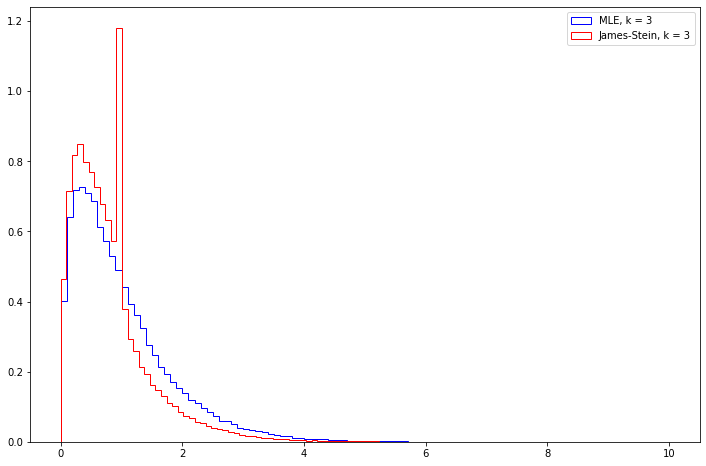
\includegraphics{Figure-13-01}
\end{figure}

\begin{figure}[H]
\centering
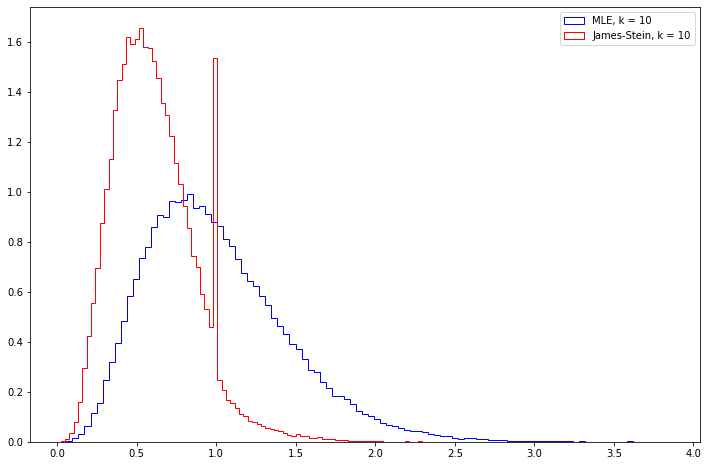
\includegraphics{Figure-13-02}
\end{figure}

\begin{figure}[H]
\centering
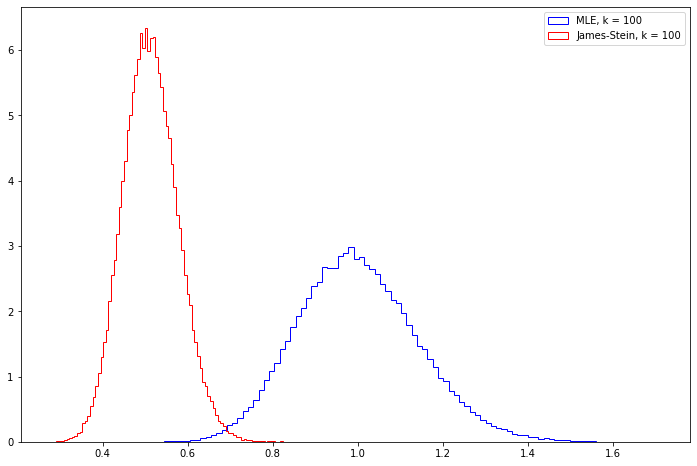
\includegraphics{Figure-13-03}
\end{figure}

\begin{figure}[H]
\centering
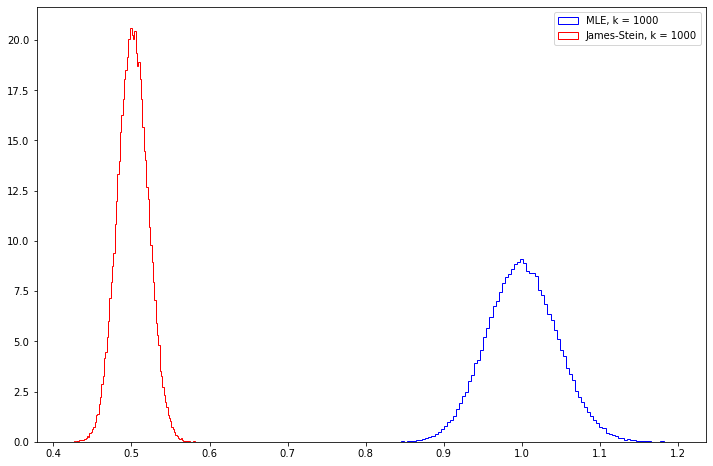
\includegraphics{Figure-13-04}
\end{figure}

Note that the James-Stein estimator seems to have its mean square error
go towards 0.5, while the MLE estimator has its error go towards 1.


% Chapter 14
\section{14. Linear Regression}\label{linear-regression}

\textbf{Regression} is a method for studying the relationship between a
\textbf{response variable} \(Y\) and a \textbf{covariates} \(X\). The
covariate is also called a \textbf{predictor variable} or
\textbf{feature}. Later we will generalize and allow for more than one
covariate. The data are of the form

\[ (Y_1, X_1), \dots, (Y_n, X_n) \]

One way to summarize the relationship between \(X\) and \(Y\) is through
the \textbf{regression function}

\[ r(x) = \mathbb{E}(Y | X = x) = \int y f(y | x) dy \]

Most of this chapter is concerned with estimating the regression
function.

\subsection{14.1 Simple Linear
Regression}\label{simple-linear-regression}

The simplest version of regression is when \(X_i\) is simple (a scalar,
not a vector) and \(r(x)\) is assumed to be linear:

\[r(x) = \beta_0 + \beta_1 x\]

This model is called the \textbf{simple linear regression model}. Let
\(\epsilon_i = Y_i - (\beta_0 + \beta_1 X_i)\). Then:

\begin{align}
\mathbb{E}(\epsilon_i | Y_i) &= \mathbb{E}(Y_i - (\beta_0 + \beta_1 X_i) | X_i)\\
&= \mathbb{E}(Y_i | X_i) - (\beta_0 + \beta_1 X_i)\\
&= r(X_i) - (\beta_0 + \beta_1 X_i)\\
&= 0
\end{align}

Let \(\sigma^2(x) = \mathbb{V}(\epsilon_i | X_i = x)\). We will make the
further simplifying assumption that \(\sigma^2(x) = \sigma^2\) does not
depend on \(x\).

\textbf{The Linear Regression Model}

\[Y_i = \beta_0 + \beta_1 X_i + \epsilon_i\]

where \(\mathbb{E}(\epsilon_i | X_i) = 0\) and
\(\mathbb{V}(\epsilon_i | X_i) = \sigma^2\).

The unknown models in the parameter are the intercept \(\beta_0\), the
slope \(\beta_1\) and the variance \(\sigma^2\). Let \(\hat{\beta_0}\)
and \(\hat{\beta_1}\) denote the estimates of \(\beta_0\) and
\(\beta_1\). The \textbf{fitted line} is defined to be

\[\hat{r}(x) = \hat{\beta}_0 + \hat{\beta}_1 x\]

The \textbf{predicted values} or \textbf{fitted values} are
\(\hat{Y}_i = \hat{r}(X_i)\) and the \textbf{residuals} are defined to
be

\[\hat{\epsilon}_i = Y_i - \hat{Y}_i = Y_i - (\hat{\beta}_0 + \hat{\beta}_1 X_i)\]

The \textbf{residual sum of squares} or RSS is defined by

\[ \text{RSS} = \sum_{i=1}^n \hat{\epsilon}_i^2\]

The quantity RSS measures how well the fitted line fits the data.

The \textbf{least squares estimates} are the values \(\hat{\beta}_0\)
and \(\hat{\beta}_1\) that minimize
\(\text{RSS} = \sum_{i=1}^n \hat{\epsilon}_i^2\).

\textbf{Theorem 14.4}. The least square estimates are given by

\begin{align}
\hat{\beta}_1 &= \frac{\sum_{i=1}^n (X_i - \overline{X}_n) (Y_i - \overline{Y}_n)}{\sum_{i=1}^n (X_i - \overline{X}_n)^2}\\
\hat{\beta}_0 &= \overline{Y}_n - \hat{\beta}_1 \overline{X}_n
\end{align}

An unbiased estimate of \(\sigma^2\) is

\[
\hat{\sigma}^2 = \left( \frac{1}{n - 2} \right) \sum_{i=1}^n \hat{\epsilon}_i^2
\]

\subsection{14.2 Least Squares and Maximum
Likelihood}\label{least-squares-and-maximum-likelihood}

Suppose we add the assumption that
\(\epsilon_i | X_i \sim N(0, \sigma^2)\), that is,

\(Y_i | X_i \sim N(\mu_i, \sigma_i^2)\)

where \(\mu_i = \beta_0 + \beta_i X_i\). The likelihood function is

\begin{align}
\prod_{i=1}n f(X_i, Y_i) &= \prod_{i=1}^n f_X(X_i) f_{Y|X}(Y_i | X_i)\\
&= \prod_{i=1}^n f_X(X_i) \times \prod_{i=1}^n f_{Y|X}(Y_i | X_i) \\
&= \mathcal{L}_1 \times \mathcal{L}_2
\end{align}

where \(\mathcal{L}_1 = \prod_{i=1}^n f_X(X_i)\) and
\(\mathcal{L}_2 = \prod_{i=1}^n f_{Y|X}(Y_i | X_i)\).

The term \(\mathcal{L}_1\) does not involve the parameters \(\beta_0\)
and \(\beta_1\). We shall focus on the second term \(\mathcal{L}_2\)
which is called the \textbf{conditional likelihood}, given by

\[\mathcal{L}_2 \equiv \mathcal{L}(\beta_0, \beta_1, \sigma)
= \prod_{i=1}^n f_{Y|X}(Y_i | X_i)
\propto \sigma^{-n} \exp \left\{ - \frac{1}{2 \sigma^2} \sum_i (Y_i - \mu_i)^2 \right\}
\]

The conditional log-likelihood is

\[\ell(\beta_0, \beta_1, \sigma) = -n \log \sigma - \frac{1}{2 \sigma^2} \sum_{i=1}^n \left(Y_i - (\beta_0 + \beta_1 X_i) \right)^2\]

To find the MLE of \((\beta_0, \beta_1)\) we maximize the conditional
log likelihood. We can see from the equation above that this is the same
as minimizing the RSS. Therefore, we have shown the following:

\textbf{Theorem 14.7}. Under the assumption of Normality, the least
squares estimator is also the maximum likelihood estimator.

We can also maximize \(\ell(\beta_0, \beta_1, \sigma)\) over \(\sigma\)
yielding the MLE

\[ \hat{\sigma}^2 = \frac{1}{n} \sum_{i=1}^n \hat{\epsilon}_i^2 \]

This estimator is similar to, but not identical to, the unbiased
estimator. Common practice is to use the unbiased estimator.

\subsection{14.3 Properties of the Least Squares
Estimators}\label{properties-of-the-least-squares-estimators}

\textbf{Theorem 14.8}. Let
\(\hat{\beta}^T = (\hat{\beta}_0, \hat{\beta}_1)^T\) denote the least
squares estimators. Then,

\[
\mathbb{E}(\hat{\beta} | X^n) = \begin{pmatrix}\beta_0 \\ \beta_1 \end{pmatrix}
\]

\[
\mathbb{V}(\hat{\beta} | X^n) = \frac{\sigma^2}{n s_X^2} \begin{pmatrix} 
\frac{1}{n} \sum_{i=1}^n X_i^2 & -\overline{X}_n \\
-\overline{X}_n & 1
\end{pmatrix}
\]

where \(s_X^2 = n^{-1} \sum_{i=1}^n (X_i - \overline{X}_n)^2\).

The estimated standard errors of \(\hat{\beta}_0\) and \(\hat{\beta}_1\)
are obtained by taking the square roots of the corresponding diagonal
terms of \(\mathbb{V}(\hat{\beta} | X^n)\) and inserting the estimate
\(\hat{\sigma}\) for \(\sigma\). Thus,

\begin{align}
\hat{\text{se}}(\hat{\beta}_0) &= \frac{\hat{\sigma}}{s_X \sqrt{n}} \sqrt{\frac{\sum_{i=1}^n X_i^2}{n}}\\
\hat{\text{se}}(\hat{\beta}_1) &= \frac{\hat{\sigma}}{s_X \sqrt{n}}
\end{align}

We should write \(\hat{\text{se}}(\hat{\beta}_0 | X^n)\) and
\(\hat{\text{se}}(\hat{\beta}_1 | X^n)\) but we will use the shorter
notation \(\hat{\text{se}}(\hat{\beta}_0)\) and
\(\hat{\text{se}}(\hat{\beta}_1)\).

\textbf{Theorem 14.9}. Under appropriate conditions we have:

\begin{enumerate}[label={\arabic*.}]
\item
  (Consistency) \(\hat{\beta}_0 \xrightarrow{\text{P}} \beta_0\) and
  \(\hat{\beta}_1 \xrightarrow{\text{P}} \beta_1\)
\item
  (Asymptotic Normality):
\end{enumerate}

\[
\frac{\hat{\beta}_0 - \beta_0}{\hat{se}(\hat{\beta}_0)} \leadsto N(0, 1)
\quad \text{and} \quad
\frac{\hat{\beta}_1 - \beta_1}{\hat{se}(\hat{\beta}_1)} \leadsto N(0, 1)
\]

\begin{enumerate}[tightlist,label={\arabic*.},resume]
\item
  Approximate \(1 - \alpha\) confidence intervals for \(\beta_0\) and
  \(\beta_1\) are
\end{enumerate}

\[
\hat{\beta}_0 \pm z_{\alpha/2} \hat{\text{se}}(\hat{\beta}_0)
\quad \text{and} \quad
\hat{\beta}_1 \pm z_{\alpha/2} \hat{\text{se}}(\hat{\beta}_1)
\]

The Wald statistic for testing \(H_0 : \beta_1 = 0\) versus
\(H_1: \beta_1 \neq 0\) is: reject \(H_0\) if \(W > z_{\alpha / 2}\)
where \(W = \hat{\beta}_1 / \hat{\text{se}}(\hat{\beta}_1)\).

\subsection{14.4 Prediction}\label{prediction}

Suppose we have estimated a regression model
\(\hat{r}(x) = \hat{\beta}_0 + \hat{\beta}_1 x\) from data
\((X_1, Y_1), \dots, (X_n, Y_n)\). We observe the value \(X_* = x\) of
the covariate for a new subject and we want to predict the outcome
\(Y_*\). An estimate of \(Y_*\) is

\[ \hat{Y}_* = \hat{\beta}_0 + \hat{\beta}_1 X_*\]

Using the formula for the variance of the sum of two random variables,

\[ \mathbb{V}(\hat{Y}_*) = \mathbb{V}(\hat{\beta}_0 + \hat{\beta}_1 x_*) = \mathbb{V}(\hat{\beta}_0) + x_* \mathbb{V}(\hat{\beta}_1) + 2 x_* \text{Cov}(\hat{\beta}_0, \hat{\beta}_1) \]

Theorem 14.8 gives the formulas for all terms in this equation. The
estimated standard error \(\hat{\text{se}}(\hat{Y}_*)\) is the square
root of this variance, with \(\hat{\sigma}^2\) in place of \(\sigma^2\).
However, \textbf{the confidence interval for \(\hat{Y}_*\) is not of the
usual form} \(\hat{Y}_* \pm z_{\alpha} \hat{\text{se}}(\hat{Y}_*)\). The
appendix explains why. The correct form is given in the following
theorem. We can the interval a \textbf{prediction interval}.

\textbf{Theorem 14.11 (Prediction Interval)}. Let

\begin{align}
\hat{\xi}_n^2 &= \hat{\text{se}}^2(\hat{Y}_*) + \hat{\sigma}^2 \\
&= \hat{\sigma}^2 \left(\frac{\sum_{i=1}^n (X_i - X_*)^2}{n \sum_{i=1}^n (X_i - \overline{X})^2} + 1 \right)
\end{align}

An approximate \(1 - \alpha\) prediction interval for \(Y_*\) is

\[ \hat{Y}_* \pm z_{\alpha/2} \xi_n\]

\subsection{14.5 Multiple Regression}\label{multiple-regression}

Now suppose we have \(k\) covariates \(X_1, \dots, X_k\). The data are
of the form

\[(Y_1, X_1), \dots, (Y_n, X_n)\]

where

\[ X_i = (X_{i1}, \dots, X_{ik}) \]

Here, \(X_i\) is the vector of \(k\) covariates for the \(i-\)th
observation. The linear regression model is

\[ Y_i = \sum_{i=1}^k \beta_j X_{ij} + \epsilon_i \]

for \(i = 1, \dots, n\) where
\(\mathbb{E}(\epsilon_i | X_{1i}, \dots, X_{ik}) = 0\). Usually we want
to include an intercept in the model which we can do by setting
\(X_{i1} = 1\) for \(i = 1, \dots, n\). At this point it will become
more convenient to express the model in matrix notation. The outcomes
will be denoted by

\[ Y = \begin{pmatrix}
Y_1 \\
Y_2 \\
\vdots \\
Y_n
\end{pmatrix}
\]

and the covariates will be denoted by

\[ X = \begin{pmatrix}
X_{11} & X_{12} & \cdots & X_{1k} \\
X_{21} & X_{22} & \cdots & X_{2k} \\
\vdots & \vdots & \ddots & \vdots \\
X_{n1} & X_{n2} & \cdots & X_{nk}
\end{pmatrix}
\]

Each row is one observation; the columns represent to the \(k\)
covariates. Thus, \(X\) is a \(n \times k\) matrix. Let

\[
\beta = \begin{pmatrix}
\beta_1 \\
\vdots \\
\beta_k
\end{pmatrix}
\quad \text{and} \quad
\epsilon = \begin{pmatrix}
\epsilon_1 \\
\vdots \\
\epsilon_k
\end{pmatrix}
\]

Then we can write the linear regression model as

\[ Y = X \beta + \epsilon \]

\textbf{Theorem 14.13}. Assuming that the \(k \times k\) matrix \(X^TX\)
is invertible, the least squares estimate is

\[ \hat{\beta} = (X^T X)^{-1} X^T Y \]

The estimated regression function is

\[ \hat{r}(x) = \sum_{j=1}^k \hat{\beta}_j x_j\]

The variance-covariance matrix of \(\hat{\beta}\) is

\[ \mathbb{V}(\hat{\beta} | X^n) = \sigma^2 (X^T X)^{-1} \]

An unbiased estimate of \(\sigma^2\) is

\[ \hat{\sigma}^2 = \left( \frac{1}{n - k} \right) \sum_{i=1}^n \hat{\epsilon}_i^2 \]

where \(\hat{\epsilon} = X \hat{\beta} - Y\) is the vector of residuals.
An approximate \(1 - \alpha\) confidence interval for \(\beta_j\) is

\[ \hat{\beta}_j \pm z_{\alpha/2} \hat{\text{se}}(\hat{\beta}_j) \]

where \(\hat{\text{se}}^2(\hat{\beta}_j)\) is the \(j\)-th diagonal
element of the matrix \(\hat{\sigma}^2 (X^T X)^{-1}\).

\subsection{14.6 Model Selection}\label{model-selection}

We may have data on many covariates but we may not want to include all
of them in the model. A smaller model with fewer covariates has two
advantages: it might give better predictions than a big model and it is
more parsimonious (simpler). Generally, as you add more variables to a
regression, the bias of the predictions decreases and the variance
increases. Too few covariates yields high bias; too many covariates
yields high variance. Good predictions result from achieving a good
balance between bias and variance.

In model selection there are two problems: assigning a score to each
model which measures, in some sense, how good the model is, and
searching through all models to find the model with the best score.

Let \(S \subset \{1, \dots, k\}\) and let
\(\mathcal{X}_S = \{ X_j : j \in S \}\) denote a subset of the
covariates. Let \(\beta_S\) denote the coefficients of the corresponding
set of covariates and let \(\hat{\beta}_S\) denote the least squares
estimate of \(\beta_S\). Let \(X_S\) denote the \(X\) matrix for this
subset of covariates, and let \(\hat{r}_S(x)\) to be the estimated
regression function. The predicted values from model \(S\) are denoted
by \(\hat{Y}_i(S) = \hat{r}_S(X_i)\).

The \textbf{prediction risk} is defined to be

\[R(S) = \sum_{i=1}^n \mathbb{E} (\hat{Y}_i(S) - Y_i^*)^2 \]

where \(Y_i^*\) denotes the value of the future observation of \(Y_i\)
at covariate value \(X_i\). Our goal is to choose \(S\) to make \(R(S)\)
small.

The \textbf{training error} is defined to be

\[\hat{R}_\text{tr}(S) = \sum_{i=1}^n (\hat{Y}_i(S) - Y_i)^2 \]

This estimate is very biased and under-estimates \(R(S)\).

\textbf{Theorem 14.15}. The training error is a downward biased estimate
of the prediction risk:

\[ \mathbb{E}(\hat{R}_\text{tr}(S)) < R(S) \]

In fact,

\[\text{bias}(\hat{R}_\text{tr}(S)) = \mathbb{E}(\hat{R}_\text{tr}(S)) - R(S) = -2 \sum_{i=1}^n \text{Cov}(\hat{Y}_i, Y_i)\]

The reason for the bias is that the data is being used twice: to
estimate the parameters and to estimate the risk. When fitting a model
with many variables, the covariance \(\text{Cov}(\hat{Y_i}, Y_i)\) will
be large and the bias of the training error gets worse.

In summary, the training error is a poor estimate of risk. Here are some
better estimates.

\textbf{Mallow's \(C_p\) statistic} is defined by

\[\hat{R}(S) = \hat{R}_\text{tr}(S) + 2 |S| \hat{\sigma}^2\]

where \(|S|\) denotes the number of terms in \(S\) and
\(\hat{\sigma}^2\) is the estimate of \(\sigma^2\) obtained from the
full model (with all covariates). Think of the \(C_p\) statistic as lack
of fit plus complexity penalty.

A related method for estimating risk is \textbf{AIC (Akaike Information
Criterion)}. The idea is to choose \(S\) to maximize

\[ \ell_S - |S|\]

where \(\ell_S\) is the log-likelihood of the model evaluated at the
MLE. In linear regression with Normal errors, maximizing AIC is
equivalent to minimizing Mallow's \(C_p\); see exercise 8.

\emph{Some texts use a slightly different definition of AIC which
involves multiplying this definition by 2 or -2. This has no effect on
which model is selected.}

Yet another method for estimating risk is \textbf{leave-one-out
cross-validation}. In this case, the risk estimator is

\[\hat{R}_\text{CV}(S) = \sum_{i=1}^n (Y_i - \hat{Y}_{(i)})^2 \]

where \(\hat{Y}_{(i)}\) is the prediction for \(Y_i\) obtained by
fitting the model with \(Y_i\) omitted. It can be shown that

\[\hat{R}_\text{CV}(S) = \sum_{i=1}^n \left( \frac{Y_i - \hat{Y}_i(S)}{1 - U_{ii}(S)} \right)^2 \]

where \(U_ii\) is the \(i\)-th diagonal element of the matrix

\[U(S) = X_S (X_S^T X_S)^{-1} X_S^T\]

Thus one need not actually drop each observation and re-fit the model.

A generalization is \textbf{k-fold cross-validation}. Here we divide the
data into \(k\) groups; often people take \(k = 10\). We omit one group
of data and fit the models on the remaining data. We use the fitted
model to predict the data in the group that was omitted. We then
estimate the risk by \(\sum_i (Y_i - \hat{Y}_i)^2\) where the sum is
over the data points in the omitted group. This process is repeated for
each of the \(k\) groups and the resulting risk estimates are averaged.

For linear regression, Mallows \(C_p\) and cross-validation often yield
essentially the same results so one might as well use Mallow's method.
In some of the more complex problems we will discuss later,
cross-validation will be more useful.

Another scoring method is \textbf{BIC (Bayesian Information Criterion)}.
Here we choose a model to maximize

\[ \text{BIC}(S) = \text{RSS}(S) = 2 |S| \hat{\sigma}^2 \]

The BIC score has a Bayesian interpretation. Let
\(\mathcal{S} = \{ S_1, \dots, S_m \}\) denote a set of models. Suppose
we assign the uniform prior \(\mathbb{P}(S_j) = 1 / m\) over the models.
Also assume we put a smooth prior on the parameters within each model.
It can be shown that the posterior probability for a model is
approximately

\[ \mathbb{P}(S_j | \text{data}) \approx \frac{e^{\text{BIC}(S_j)}}{\sum_r e^{\text{BIC}(S_r)}}\]

so choosing the model with highest BIC is like choosing the model with
highest posterior probability.

The BIC score also has an information-theoretical interpretation in
terms of something called minimum description length.

The BIC score is identical to Mallows \(C_p\) except that it puts a more
severe penalty for complexity. It thus leads one to choose a smaller
model than the other methods.

If there are \(k\) covariates then there are \(2^k\) possible models. We
need to search through all of those models, assign a score to each one,
and choose the model with the best score. When \(k\) is large, this is
infeasible; in that case, we need to search over a subset of all the
models. Two common methods are \textbf{forward and backward stepwise
regression}.

In forward stepwise regression, we start with no covariates in the
model, and keep adding variables one at a time that lead to the best
score. In backward stepwise regression, we start with the biggest model
(all covariates) and drop one variable at a time.

\subsection{14.7 The Lasso}\label{the-lasso}

This method, due to Tibshirani, is called the \textbf{Lasso}. Assume
that all covariates have been rescaled to have the same variance.
Consider estimating \(\beta = (\beta_1, \dots, \beta_k)\) by minimizing
the loss function

\[ \sum_{i=1}^n (Y_i - \hat{Y}_i)^2 + \lambda \sum_{j=1}^k | \beta_j |\]

where \(\lambda > 0\). The idea is to minimize the sums of squares but
there is a penalty that gets large if any \(\beta_j\) gets large. It can
be shown that some of the \(\beta_j\)'s will be 0. We interpret this as
having the \(j\)-th covariate omitted from the model; thus we are doing
estimation and model selection simultaneously.

We need to choose a value of \(\lambda\). We can do this by estimating
the prediction risk \(R(\lambda)\) as a function of \(\lambda\) and
choosing to minimize it. For example, we can estimate the risk using
leave-one-out cross-validation

\subsection{14.8 Technical Appendix}\label{technical-appendix}

The prediction interval is of a different form than other confidence
intervals we have seen -- the quantity of interest \(Y_*\) is equal to a
parameter \(\theta\) plus a random variable.

We can fix this by defining:

\[ \xi_n^2 = \mathbb{V}(\hat{Y}_*) + \sigma^2 = \left[\frac{\sum_i (x_i - x_*)^2}{n \sum_i (x_i - \overline{x})^2} + 1\right] \sigma^2\]

In practice, we substitute \(\hat{\sigma}\) for \(\sigma\) and we denote
the resulting quantity by \(\hat{\xi}_n\). Now,

\begin{align}
\mathbb{P}(\hat{Y}_* - z_{\alpha/2} \hat{\xi}_n < Y_* < \hat{Y}_* + z_{\alpha/2} \hat{\xi}_n) &=
\mathbb{P}\left(-z_{\alpha/2} < \frac{\hat{Y}_* - Y_*}{\hat{\xi}_n} < z_{\alpha/2} \right)\\
&= \mathbb{P}\left(-z_{\alpha/2} < \frac{\hat{\theta} - \theta - \epsilon}{\hat{\xi}_n} < z_{\alpha/2} \right) \\
&\approx \mathbb{P}\left(-z_{\alpha/2} < \frac{N(0, s^2 + \sigma^2)}{\hat{\xi}_n} < z_{\alpha/2} \right)  \\
&\approx \mathbb{P}\left(-z_{\alpha/2} < \frac{N(0, s^2 + \sigma^2)}{\xi_n} < z_{\alpha/2} \right)  \\
&= \mathbb{P}(-z_{\alpha/2} < N(0, 1) < z_{\alpha/2}) \\
&= 1 - \alpha
\end{align}

\subsection{14.9 Exercises}\label{exercises}

\textbf{Exercise 14.9.1}. Prove Theorem 14.4:

The least square estimates are given by

\begin{align}
\hat{\beta}_1 &= \frac{\sum_{i=1}^n (X_i - \overline{X}_n) (Y_i - \overline{Y}_n)}{\sum_{i=1}^n (X_i - \overline{X}_n)^2}\\
\hat{\beta}_0 &= \overline{Y}_n - \hat{\beta}_1 \overline{X}_n
\end{align}

An unbiased estimate of \(\sigma^2\) is

\[
\hat{\sigma}^2 = \left( \frac{1}{n - 2} \right) \sum_{i=1}^n \hat{\epsilon}_i^2
\]

\textbf{Solution}. We can obtain the estimates \(\hat{\beta}_0\) and
\(\hat{\beta}_1\) by minimizing the RSS -- by taking the partial
derivatives with respect to \(\beta_0\) and \(\beta_1\):

\[\text{RSS} = \sum_i \hat{\epsilon}_i^2 = \sum_i (Y_i - (\beta_0 + \beta_1 X_i))^2\]

Derivating RSS on \(\beta_0\):

\[\frac{d}{d \beta_0}\text{RSS} = \sum_i \frac{d}{d \beta_0} (Y_i - (\beta_0 + \beta_1 X_i))^2
= \sum_i 2 (\beta_0 - (Y_i - \beta_1 X_i))\]

Making this derivative equal to 0 at \(\hat{\beta}_0\),
\(\hat{\beta}_1\) gives:

\begin{align}
0 &= \sum_i 2 (\hat{\beta}_0 - (Y_i - \hat{\beta}_1 X_i))\\
n \hat{\beta}_0 &= n \sum_i Yi - \hat{\beta}_1 n \sum_i X_i\\
\hat{\beta}_0 &= \overline{Y}_n - \hat{\beta}_1 \overline{X}_n
\end{align}

Replacing \(\overline{Y}_n - \beta_1 \overline{X}_n\) for \(\beta_0\)
and derivating on \(\beta_1\):

\[\frac{d}{d \beta_1}\text{RSS} = \sum_i \frac{d}{d \beta_1} (Y_i - (\beta_0 + \beta_1 X_i))^2
\sum_i \frac{d}{d \beta_1} (Y_i - \overline{Y}_n - \beta_1 (X_i - \overline{X}_n)))^2
= \sum_i -2 (X_i - \overline{X}_n) (Y_i - \overline{Y}_n - \beta_1 (X_i - \overline{X}_n)))\]

Making this derivative equal to 0 at \(\hat{\beta}_1\) gives:

\begin{align}
0 &= \sum_i (X_i - \overline{X}_n) (Y_i - \overline{Y}_n - \beta_1 (X_i - \overline{X}_n))) \\
0 &= \hat{\beta}_1 \sum_i (\overline{X}_n - X_i)^2 + \sum_i (\overline{X}_n - X_i)(Y_i - \overline{Y}_n) \\
\hat{\beta}_1 &= \frac{\sum_i (X_i - \overline{X}_n)(Y_i - \overline{Y}_n)}{\sum_i (X_i - \overline{X}_n)^2}
\end{align}

For the unbiased estimate, let's adapt a more general proof from Greene
(2003), restricted to \(k = 2\) dimensions, where the first dimension is
set to all ones to represent the intercept, and the second dimension
represents the one-dimensional covariates \(X_i\).

The vector of least square residuals is

\[ \hat{\epsilon} = \begin{pmatrix}
\hat{\epsilon}_1 \\
\hat{\epsilon}_2 \\
\vdots \\
\hat{\epsilon}_n
\end{pmatrix} = \begin{pmatrix}
Y_1 - (\hat{\beta}_0 \cdot 1 + \hat{\beta}_1 X_1) \\
Y_2 - (\hat{\beta}_0 \cdot 1 + \hat{\beta}_1 X_2) \\
\vdots \\
Y_n - (\hat{\beta}_0 \cdot 1 + \hat{\beta}_1 X_n)
\end{pmatrix} = 
y - X \hat{\beta}
\]

where \[
y = \begin{pmatrix}
Y_1 \\
Y_2 \\
\vdots \\
Y_n
\end{pmatrix}
, \quad
X = \begin{pmatrix}
1 & X_1 \\
1 & X_2 \\
\vdots & \vdots \\
1 & X_n
\end{pmatrix},
\quad \text{and} \quad
\hat{\beta} = \begin{pmatrix}
\hat{\beta}_0 \\
\hat{\beta}_1
\end{pmatrix}
\]

The least squares solution can be written as:

\[\hat{\beta} = (X^T X)^{-1} X^T y\]

Replacing it on the definition of \(\hat{\epsilon}\), we get

\[ \hat{\epsilon} = y - X (X^T X)^{-1} X^T y = (I - X (X^T X)^{-1} X^T) y = M y\]

where \(M = I - X (X^T X)^{-1} X^T\) is known as the \textbf{residual
maker} matrix.

Note that \(M\) is symmetric, that is, \(M^T = M\):

\begin{align}
M^T &= (I - X (X^T X)^{-1} X^T)^T  \\
&= I^T - (X (X^T X)^{-1} X^T)^T \\
&= I - (X^T)^T ((X^T X)^{-1})^T X^T \\
&= I - X ((X^{-1}(X^T)^{-1})^T X^T \\
&= I -  X (X^T X)^{-1} X^T \\
&= M
\end{align}

Note also that \(M\) is idempotent, that is, \(M^2 = M\):

\begin{align}
M^2 &= (I - X (X^T X)^{-1} X^T) (I - X (X^T X)^{-1} X^T) \\
&= I - X (X^T X)^{-1} X^T - X (X^T X)^{-1} X^T + X \left( (X^T X)^{-1} X^T X \right) (X^T X)^{-1} X^T \\
&= I - X (X^T X)^{-1} X^T - X (X^T X)^{-1} X^T + X (X^T X)^{-1} X^T \\
&= I - X (X^T X)^{-1} X^T \\
&= M
\end{align}

Now, we have that \(MX = 0\), as running least squares on a regression
where the covariates match the target variables should yield a model
that just copies the covariate over, where all residuals are zero
(\(\beta_0 = 0\) and \(\beta_1 = 1\)). So:

\[\hat{\epsilon} = M y = M( X \beta + \epsilon) = M\epsilon\]

where \(\epsilon = Y - X\beta\) are the population residuals.

We can then write an estimator for \(\sigma^2\):

\[ \hat{\epsilon}^T \hat{\epsilon} = \epsilon^T M^T M \epsilon = \epsilon^T M^2 \epsilon = \epsilon^T M \epsilon\]

Taking the expectation with respect to the data \(X\) on both sides,

\[\mathbb{E}(\hat{\epsilon}^T \hat{\epsilon} | X) = \mathbb{E}(\epsilon^T M \epsilon | X)\]

But \(\epsilon^T M \epsilon\) is a scalar (\(1 \times 1\) matrix), so it
is equal to its trace -- and we can use the cyclic permutation property
of the trace:

\[ \mathbb{E}(\epsilon^T M \epsilon | X) = \mathbb{E}(\text{tr}(\epsilon^T M \epsilon) | X) = \mathbb{E}(\text{tr}(M \epsilon \epsilon^T) | X)\]

Since \(M\) is a function of \(X\), we can take it out of the
expectation:

\[\mathbb{E}(\text{tr}(M \epsilon \epsilon^T) | X) = \text{tr}(\mathbb{E}(M \epsilon \epsilon^T | X))
= \text{tr}(M \mathbb{E}(\epsilon \epsilon^T | X))
= \text{tr}(M \sigma^2 I_1)
= \sigma^2 \text{tr}(M)
\]

Finally, we can compute the trace of \(M\):

\begin{align}
\text{tr}(M) &= \text{tr}(I_n - X(X^T X)^{-1}X^T)\\
&= \text{tr}(I_n) - \text{tr}(X(X^T X)^{-1}X^T) \\
&= \text{tr}(I_n) - \text{tr}((X^T X)^{-1}X^T X) \\
&= \text{tr}(I_n) - \text{tr}(I_k)  \\
&= n - k
\end{align}

Therefore, the unbiased estimator is

\[\hat{\sigma}^2 = \frac{\hat{\epsilon}^T \hat{\epsilon}}{n - k}\]

or, for our case where \(k = 2\),

\[\hat{\sigma}^2 = \left( \frac{1}{n - 2} \right) \sum_{i=1}^n \hat{\epsilon}_i^2\]

Reference: Greene, William H. Econometric analysis. Pearson Education
India, 2003. Chapter 4, pages 61-62.

\textbf{Exercise 14.9.2}. Prove the formulas for the standard errors in
Theorem 14.8. You should regard the \(X_i\)'s as fixed constants.

\[
\mathbb{E}(\hat{\beta} | X^n) = \begin{pmatrix}\beta_0 \\ \beta_1 \end{pmatrix}
\quad \text{and} \quad
\mathbb{V}(\hat{\beta} | X^n) = \frac{\sigma^2}{n s_X^2} \begin{pmatrix} 
\frac{1}{n} \sum_{i=1}^n X_i^2 & -\overline{X}_n \\
-\overline{X}_n & 1
\end{pmatrix}
\]

\[s_X^2 = n^{-1} \sum_{i=1}^n (X_i - \overline{X}_n)^2\]

\[
\hat{\text{se}}(\hat{\beta}_0) = \frac{\hat{\sigma}}{s_X \sqrt{n}} \sqrt{\frac{\sum_{i=1}^n X_i^2}{n}}
\quad \text{and} \quad
\hat{\text{se}}(\hat{\beta}_1) = \frac{\hat{\sigma}}{s_X \sqrt{n}}
\]

\textbf{Solution}.

The formulas follow immediately by performing the suggested replacement
on the diagonal elements of \(\mathbb{V}(\hat{\beta} | X^n)\) from
Theorem 14.8. From the diagonals, replacing \(\hat{\sigma}\) for
\(\sigma\):

\[
\hat{\text{se}}(\hat{\beta}_0)^2 = \frac{\hat{\sigma}^2}{n s_X^2} \frac{\sum_{i=1}^n X_i^2}{n}
\quad \text{and} \quad
\hat{\text{se}}(\hat{\beta}_1)^2 = \frac{\hat{\sigma}^2}{n s_X^2} \cdot 1\]

Results follow by taking the square root.

We will also prove the variance matrix result itself, following from the
notation and proof used on exercise 14.9.1 (again, adapting from
Greene):

\[
\hat{\beta} = (X^T X)^{-1}X^T y = (X^T X)^{-1}X^T (X \beta + \epsilon) = \beta + (X^T X)^{-1}X^T \epsilon
\]

Taking the variance conditional on \(X\),

\begin{align}
\mathbb{V}(\hat{\beta} | X) &= \mathbb{V}(\hat{\beta} - \beta | X) \\
&= \mathbb{E}((\hat{\beta} - \beta)(\hat{\beta} - \beta)^T | X)  \\
&= \mathbb{E}((X^T X)^{-1}X^T \epsilon\epsilon^T X(X^T X)^{-1} | X) \\
&= (X^T X)^{-1}X^T \mathbb{E}(\epsilon\epsilon^T | X) X(X^T X)^{-1} \\
&= (X^T X)^{-1}X^T \sigma^2 I X(X^T X)^{-1} \\
&= \sigma^2 (X^T X)^{-1} 
\end{align}

But we have:

\[ X^T X = \begin{pmatrix}
1 & 1 & \cdots & 1 \\
X_1 & X_2 & \cdots & X_n
\end{pmatrix} \begin{pmatrix}
1 & X_1 \\
1 & X_2 \\
\vdots & \vdots \\
1 & X_n
\end{pmatrix} = 
n \begin{pmatrix}
1 & \overline{X}_n \\
\overline{X}_n & \frac{1}{n}\sum_{i=1}^n X_i^2
\end{pmatrix}
\]

so we can verify its inverse is

\[(X^T X)^{-1} = \frac{1}{n s_X^2} \begin{pmatrix}
\frac{1}{n} \sum_{i=1}^n X_i^2 & - \overline{X}_n \\
-\overline{X}_n & 1
\end{pmatrix}\]

and so the result follows.

Reference: Greene, William H. Econometric analysis. Pearson Education
India, 2003. Chapter 4, page 59.

\textbf{Exercise 14.9.3}. Consider the \textbf{regression through the
origin} model:

\[Y_i = \beta X_i + \epsilon\]

Find the least squares estimate for \(\beta\). Find the standard error
of the estimate. Find conditions that guarantee that the estimate is
consistent.

\textbf{Solution}. Once more adopting notation from the solution of
14.9.1, let

\[ y = \begin{pmatrix} Y_1 \\ \vdots \\ Y_n \end{pmatrix},
\quad
X = \begin{pmatrix} X_1 \\ \vdots \\ X_n \end{pmatrix}\]

and \(\beta\) is a scalar (or a \(1 \times 1\) matrix).

The least squares estimate is, again,

\[\hat{\beta} = (X^T X)^{-1} X^T y\]

which simplifies in this one-dimensional case to:

\[\hat{\beta} = \frac{\sum_{i=1}^n X_i Y_i}{\sum_{i=1}^n X_i^2}\]

The unbiased estimator for \(\sigma^2\) is, with \(k = 1\),

\[\hat{\sigma}^2 = \frac{1}{n - 1} \sum_{i=1}^n \hat{\epsilon}_i^2\]

and the variance of \(\hat{\beta}\) conditional of \(X\) is:

\[\mathbb{V}(\hat{\beta} | X) = \sigma^2 (X^T X)^{-1} = \frac{\sigma^2}{\sum_{i=1}^n X_i^2}\]

so the standard error of the estimate is

\[\hat{\text{se}}(\hat{\beta}) = \frac{\hat{\sigma}}{\sqrt{\sum_{i=1}^n X_i^2}}\]

These, of course, make the assumption that \(X^T X\) is invertible --
that is, that the sum of squares of the \(X_i\) variables is greater
than 0. This is only not the case when all covariates are 0, in which
case the value of our estimator \(\hat{\beta}\) would be irrelevant to
determining the prediction outcome -- the system would be undetermined.

Finally, note that \(\hat{\beta}\) is also the MLE in the parameter
space for regression through the origin. As each measurement error
\(\epsilon_i = Y_i - \beta X_i\) is drawn from a normal distribution
\(N(0, \sigma^2)\), the log-likelihood for a given parameter \(\beta\)
is

\[\ell_n(\beta) = -\frac{n}{2} \log \sigma^2 - \frac{1}{2 \sigma^2} \sum_{i=1}^n (Y_i - \beta X_i)^2 + C\]

and so maximizing it is equivalent to minimizing
\(\sum_{i=1}^n (Y_i - \beta X_i)^2\), which is what the least squares
procedure does.

Since the MLE is consistent, the least squares estimate is also
consistent.

\textbf{Exercise 14.9.4}. Prove equation (14.24).

\[ \text{bias}(\hat{R}_\text{tr}(S)) = \mathbb{E}(\hat{R}_\text{tr}(S)) - R(S) = -2 \sum_i \text{Cov}(\hat{Y}_i, Y_i) \]

\textbf{Solution}.

The bias is:

\begin{align}
\mathbb{E}(\hat{R}_\text{tr}(S)) - R(S) &= \mathbb{E}\left[\sum_i (\hat{Y}_i- Y_i)^2 \right] - \mathbb{E} \left[ \sum_i (\hat{Y}_i - Y_i^*)^2 \right] \\
&= \sum_i \left( \mathbb{E} \left[\hat{Y}_i^2 \right] - 2 \mathbb{E} \left[\hat{Y}_i Y_i \right] + \mathbb{E}\left[Y_i^2 \right] - \mathbb{E} \left[\hat{Y}_i^2 \right] + 2 \mathbb{E} \left[\hat{Y}_i Y_i^* \right] - \mathbb{E}\left[{Y_i^*}^2 \right] \right)
\end{align}

The random variables \(Y_i = \beta X_i + \epsilon_\text{train}\) and
\(Y_i^* = \beta X_i + \epsilon_\text{pred}\) are independent, as the
errors during training and predition are independent, and the covariates
\(X_i\) and true parameter \(\beta\) are constant. Since they are
independent,
\(\mathbb{E}[Y_i Y_i^*] = \mathbb{E}[Y_i] \mathbb{E}[Y_i^*]\).

We also have
\(\mathbb{E} [ {Y_i^*}^2 ] = \mathbb{V}[Y_i^*] + \mathbb{E}[Y_i^*]^2 = \mathbb{V}[\epsilon_\text{pred}] + \mathbb{E}[X \beta]^2 = \mathbb{V}[\epsilon_\text{train}] + \mathbb{E}[Y_i]^2 = \mathbb{E} [Y_i^2]\).

Replacing both of those in the expression of bias above, we get the
result:

\begin{align}
\mathbb{E}(\hat{R}_\text{tr}(S)) - R(S) &= 
-2 \sum_i \left( \mathbb{E}[Y_i \hat{Y}_i] - \mathbb{E}[Y_i] \mathbb{E}[\hat{Y}_i] \right) \\
&= -2 \sum_i \text{Cov}(\hat{Y}_i, Y_i)
\end{align}

\textbf{Exercise 14.9.5}. In the simple linear regression model,
construct a Wald test for \(H_0 : \beta_1 = 17 \beta_0\) versus
\(H_1 : \beta_1 \neq 17 \beta_0\).

\textbf{Solution}. Let \(\delta = \beta_1 - 17 \beta_0\). The MLE is
\(\hat{\delta} = \hat{\beta}_1 - 17 \hat{\beta}_0\), with estimated
standard error \(\hat{\text{se}}(\hat{\delta})\), where

\[\hat{\text{se}}(\hat{\delta})^2 = \hat{\text{se}}(\hat{\beta}_1 - 17 \hat{\beta}_0)^2 = \hat{\text{se}}(\hat{\beta}_1)^2 + 17^2 \hat{\text{se}}(\hat{\beta}_0)^2 \]

and the estimates for the parameter standard deviations are

\[
\hat{\text{se}}(\hat{\beta}_0) = \frac{\hat{\sigma}}{s_X \sqrt{n}} \sqrt{\frac{\sum_{i=1}^n X_i^2}{n}}
\quad \text{and} \quad
\hat{\text{se}}(\hat{\beta}_1) = \frac{\hat{\sigma}}{s_X \sqrt{n}}
\]

The Wald test then checks if \(|W| < z_{\alpha / 2}\), where

\[W = \frac{\hat{\delta} - 0}{\hat{\text{se}}(\hat{\delta})} 
= \frac{\hat{\beta}_1 - 17 \hat{\beta}_0}{\sqrt{\hat{\text{se}}(\hat{\beta}_1)^2 + 17^2 \hat{\text{se}}(\hat{\beta}_0)^2}}\]

\textbf{Exercise 14.9.6}. Get the passenger car mileage data from

http://lib.stat.cmu.edu/DASL/Datafiles/carmpgdat.html

\textbf{(a)} Fit a simple linear regression model to predict MPG (miles
per gallon) from HP (horsepower). Summarize your analysis including a
plot of the data with the fitted line.

\textbf{(b)} Repeat the analysis but use log(MPG) as the response.
Compare the analysis.

\textbf{Solution}.

We would ordinarily use a library to do linear regression, but given
this chapter is specifically on linear regression formulas, let's do all
of the calculations on matrix algebra ``by hand'' instead -- and compare
the results with statsmodels OLS.

\begin{python}
import numpy as np
import pandas as pd
from scipy.stats import t
import statsmodels.api as sm
import matplotlib.pyplot as plt

# Provided link is dead.  Data was found elsewhere online.
data = pd.read_csv('data/carmileage.csv')
\end{python}

\begin{python}
def get_regression(X, Y):
    X = X.copy()
    
    # Create new column with all 1s for intercept at start
    X.insert(0, 'const', 1)
    
    # Least squares solution
    beta_hat = (np.linalg.inv(X.T @ X) @ X.T @ Y).to_numpy()

    # Predicted solutions
    Y_pred = X @ beta_hat

    # Prediction errors
    epsilon_hat = Y_pred - Y

    # Error on training data
    training_error = epsilon_hat.T @ epsilon_hat
    
    # Estimated error variance
    sigma2_hat = (training_error / (Y.shape[0] - X.shape[1]))

    # Parameter estimated standard errors
    se_beta_hat = np.sqrt(sigma2_hat * np.diag(np.linalg.inv(X.T @ X))).T

    # t statistic for estimated parameters being non-zero
    t_values = beta_hat.reshape(-1) / se_beta_hat

    # p-values for estimated parameters being non-zero
    p_values = 2 * (1 - t.cdf(np.abs(t_values), X.shape[0] - 1))
    
    return pd.DataFrame({
        'coef': beta_hat.reshape(-1),
        'std err': se_beta_hat.reshape(-1),
        't': t_values.reshape(-1),
        'P > |t|': p_values.reshape(-1) 
        }, index=X.columns)
\end{python}


\textbf{(a)}

\begin{python}
Y = data['MPG']
X = data[['HP']]
\end{python}

\begin{python}
# Using manually coded solution
get_regression(X, Y)
\end{python}

\begin{console}
	coef	std err	t	P > |t|
const	50.066078	1.569487	31.899650	0.0
HP	-0.139023	0.012069	-11.519295	0.0
\end{console}

\begin{python}
# Using statsmodels
results = sm.OLS(Y, sm.add_constant(X)).fit()
print(results.summary())
\end{python}

\begin{console}
                            OLS Regression Results
==============================================================================
Dep. Variable:                    MPG   R-squared:                       0.624
Model:                            OLS   Adj. R-squared:                  0.619
Method:                 Least Squares   F-statistic:                     132.7
Date:                Sun, 15 Mar 2020   Prob (F-statistic):           1.15e-18
Time:                        17:06:26   Log-Likelihood:                -264.61
No. Observations:                  82   AIC:                             533.2
Df Residuals:                      80   BIC:                             538.0
Df Model:                           1
Covariance Type:            nonrobust
==============================================================================
                 coef    std err          t      P>|t|      [0.025      0.975]
------------------------------------------------------------------------------
const         50.0661      1.569     31.900      0.000      46.943      53.189
HP            -0.1390      0.012    -11.519      0.000      -0.163      -0.115
==============================================================================
Omnibus:                       22.759   Durbin-Watson:                   0.721
Prob(Omnibus):                  0.000   Jarque-Bera (JB):               31.329
Skew:                           1.246   Prob(JB):                     1.57e-07
Kurtosis:                       4.722   Cond. No.                         299.
==============================================================================

Warnings:
[1] Standard Errors assume that the covariance matrix of the errors is correctly
specified.
\end{console}

\begin{python}
# Plotting results

fig, ax = plt.subplots(figsize=(12, 8))
fig = sm.graphics.plot_fit(results, 1, ax=ax)
plt.show()
\end{python}

\begin{figure}[H]
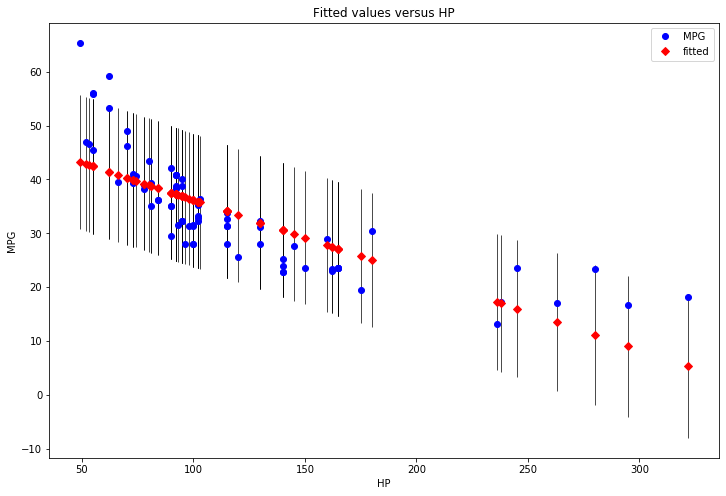
\includegraphics[width=0.9\linewidth,height=0.2\textheight,keepaspectratio]{Figure-14-01}
\end{figure}

\textbf{(b)}

\begin{python}
# Exactly the same exercise, but fit on a different response variable

Y = np.log(data['MPG']).rename('log MPG')
X = data[['HP']]
\end{python}

\begin{python}
# Using manually coded solution
get_regression(X, Y)
\end{python}

\begin{console}
	coef	std err	t	P > |t|
const	4.013229	0.040124	100.021194	0.0
HP	-0.004589	0.000309	-14.873129	0.0
\end{console}

\begin{python}
# Using statsmodels
results = sm.OLS(Y, sm.add_constant(X)).fit()
print(results.summary())
\end{python}

\begin{console}
                            OLS Regression Results
==============================================================================
Dep. Variable:                log MPG   R-squared:                       0.734
Model:                            OLS   Adj. R-squared:                  0.731
Method:                 Least Squares   F-statistic:                     221.2
Date:                Sun, 15 Mar 2020   Prob (F-statistic):           9.62e-25
Time:                        17:06:26   Log-Likelihood:                 36.047
No. Observations:                  82   AIC:                            -68.09
Df Residuals:                      80   BIC:                            -63.28
Df Model:                           1
Covariance Type:            nonrobust
==============================================================================
                 coef    std err          t      P>|t|      [0.025      0.975]
------------------------------------------------------------------------------
const          4.0132      0.040    100.021      0.000       3.933       4.093
HP            -0.0046      0.000    -14.873      0.000      -0.005      -0.004
==============================================================================
Omnibus:                        4.454   Durbin-Watson:                   1.026
Prob(Omnibus):                  0.108   Jarque-Bera (JB):                3.827
Skew:                           0.516   Prob(JB):                        0.148
Kurtosis:                       3.236   Cond. No.                         299.
==============================================================================

Warnings:
[1] Standard Errors assume that the covariance matrix of the errors is correctly
specified.
\end{console}

\begin{python}
# Plotting results

fig, ax = plt.subplots(figsize=(12, 8))
fig = sm.graphics.plot_fit(results, 1, ax=ax)
plt.show()
\end{python}

\begin{figure}[H]
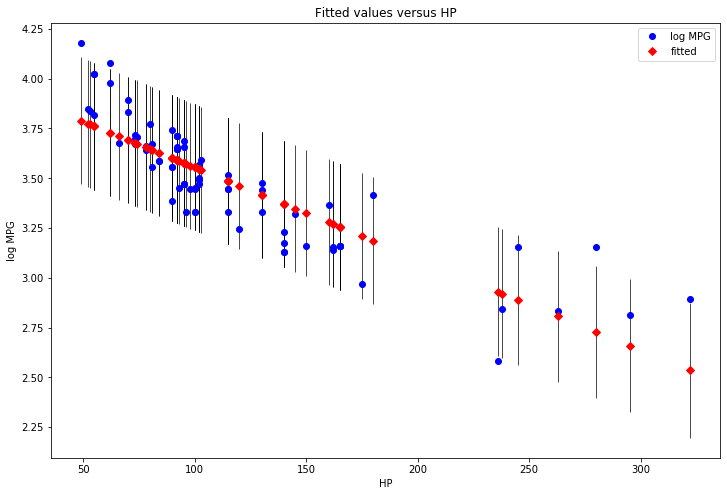
\includegraphics[width=0.9\linewidth,height=0.2\textheight,keepaspectratio]{Figure-14-02}
\end{figure}

\textbf{Exercise 14.9.7}. Get the passenger car mileage data from

http://lib.stat.cmu.edu/DASL/Datafiles/carmpgdat.html

\textbf{(a)} Fit a multiple linear regression model to predict MPG
(miles per gallon) from HP (horsepower). Summarize your analysis
including a plot of the data with the fitted line.

\textbf{(b)} Use Mallow's \(C_p\) to select a best sub-model. To search
through all models try (i) all possible models, (ii) forward stepwise,
(iii) backward stepwise. Summarize your findings.

\textbf{(c)} Repeat (b) but use BIC. Compare the results.

\textbf{(d)} Now use Lasso and compare the results.

\textbf{Solution}.

The exercise wording is unclear -- if we specify that HP is the only
covariate, the multiple linear regression and the simple linear
regression are the same, and (a) is like the previous exercise.

We will elect to use VOL, HP, SP and WT as the covariates, and MPG as
the response variable.

\textbf{(a)}

\begin{python}
# Use full model

features = ['HP', 'SP', 'WT', 'VOL']

Y = data['MPG']
X = data[features]
\end{python}

\begin{python}
# Using manually coded solution
get_regression(X, Y)
\end{python}

\begin{console}
             coef    std err         t       P > |t|
const  192.437753  23.531613  8.177839  3.351097e-12
HP       0.392212   0.081412  4.817602  6.671547e-06
SP      -1.294818   0.244773 -5.289864  1.019119e-06
WT      -1.859804   0.213363 -8.716617  2.888800e-13
VOL     -0.015645   0.022825 -0.685425  4.950327e-01
\end{console}
        
\begin{python}
# Using statsmodels
results = sm.OLS(Y, sm.add_constant(X)).fit()
print(results.summary())
\end{python}

\begin{console}
                            OLS Regression Results
==============================================================================
Dep. Variable:                    MPG   R-squared:                       0.873
Model:                            OLS   Adj. R-squared:                  0.867
Method:                 Least Squares   F-statistic:                     132.7
Date:                Sun, 15 Mar 2020   Prob (F-statistic):           9.98e-34
Time:                        17:06:27   Log-Likelihood:                -220.00
No. Observations:                  82   AIC:                             450.0
Df Residuals:                      77   BIC:                             462.0
Df Model:                           4
Covariance Type:            nonrobust
==============================================================================
                 coef    std err          t      P>|t|      [0.025      0.975]
------------------------------------------------------------------------------
const        192.4378     23.532      8.178      0.000     145.580     239.295
HP             0.3922      0.081      4.818      0.000       0.230       0.554
SP            -1.2948      0.245     -5.290      0.000      -1.782      -0.807
WT            -1.8598      0.213     -8.717      0.000      -2.285      -1.435
VOL           -0.0156      0.023     -0.685      0.495      -0.061       0.030
==============================================================================
Omnibus:                       14.205   Durbin-Watson:                   1.148
Prob(Omnibus):                  0.001   Jarque-Bera (JB):               18.605
Skew:                           0.784   Prob(JB):                     9.12e-05
Kurtosis:                       4.729   Cond. No.                     1.16e+04
==============================================================================

Warnings:
[1] Standard Errors assume that the covariance matrix of the errors is correctly
specified.
[2] The condition number is large, 1.16e+04. This might indicate that there are
strong multicollinearity or other numerical problems.
\end{console}

\begin{python}
# Plotting results

fig, ax = plt.subplots(figsize=(12, 8))
fig = sm.graphics.plot_fit(results, 1, ax=ax)
ax.set_ylabel("MPG")
ax.set_xlabel("HP")
ax.set_title("Linear Regression")
plt.show()
\end{python}

\begin{figure}[H]
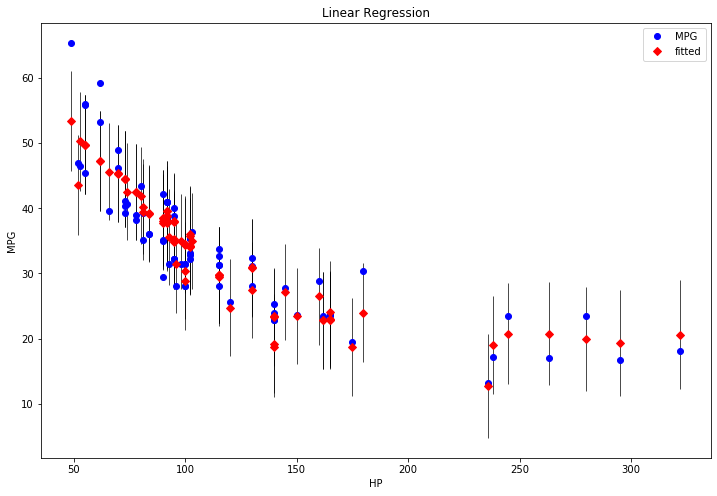
\includegraphics[width=0.9\linewidth,height=0.2\textheight,keepaspectratio]{Figure-14-03}
\end{figure}

\textbf{(b)}

First, let's create helper functions to calculate the model variance and
Mallow's \(C_p\):

\begin{python}
def get_model_variance(X, Y):
    X = X.copy()
    
    # Create new column with all 1s for intercept at start
    X.insert(0, 'const', 1)
    
    # Least squares solution
    beta_hat = (np.linalg.inv(X.T @ X) @ X.T @ Y).to_numpy()

    # Predicted solutions
    Y_pred = X @ beta_hat

    # Prediction errors
    epsilon_hat = Y_pred - Y

    # Error on training data
    training_error = epsilon_hat.T @ epsilon_hat
    
    # Estimated error variance
    return (training_error / (Y.shape[0] - X.shape[1]))
    

def get_mallow_cp(X, Y, S, full_model_variance):
    if len(S) > 0:
        X = X[list(S)].copy()
        # Create new column with all 1s for intercept at start
        X.insert(0, 'const', 1)
    else:
        X = pd.DataFrame({'const': np.ones_like(Y)})
    
    # Least squares solution
    beta_hat = (np.linalg.inv(X.T @ X) @ X.T @ Y).to_numpy()

    # Predicted solutions
    Y_pred = X @ beta_hat

    # Prediction errors
    epsilon_hat = Y_pred - Y

    # Error on training data
    partial_training_error = epsilon_hat.T @ epsilon_hat
    
    # Increase size of S by to account for constant covariate
    return partial_training_error + 2 * (len(S) + 1) * full_model_variance
\end{python}

Next, let's calculate and save the full model variance \textbf{once},
sine it's used for every candidate model -- and use it to define our
custom score function.

\begin{python}
full_model_variance = get_model_variance(X, Y)

def score_mallow_cp(S):
    return get_mallow_cp(X, Y, S, full_model_variance)
\end{python}

Finally, let's do the submodel search.

First approach is an explicit search through all features:

\begin{python}
# Recipe from itertools documentation, https://docs.python.org/2.7/library/itertools.html#recipes

from itertools import chain, combinations

def powerset(iterable):
    "powerset([1,2,3]) --> () (1,) (2,) (3,) (1,2) (1,3) (2,3) (1,2,3)"
    s = list(iterable)
    return chain.from_iterable(combinations(s, r) for r in range(len(s)+1))
\end{python}

\begin{python}
# Iterate through the powerset and calculate the score for each value
results = [(S, score_mallow_cp(S)) for S in powerset(features)]
    
# Format as dataframe for ease of presentation
results = pd.DataFrame(results, columns=['S', 'score'])
\end{python}

\begin{python}
results
\end{python}

\begin{console}
                    S        score
0                  ()  8134.147794
1               (HP,)  3102.805578
2               (SP,)  4318.234609
3               (WT,)  1519.372094
4              (VOL,)  7059.223052
5            (HP, SP)  2436.578842
6            (HP, WT)  1510.677511
7           (HP, VOL)  2354.823180
8            (SP, WT)  1463.076513
9           (SP, VOL)  3056.598857
10          (WT, VOL)  1542.174631
11       (HP, SP, WT)  1140.390871
12      (HP, SP, VOL)  2147.886521
13      (HP, WT, VOL)  1507.484328
14      (SP, WT, VOL)  1443.795004
15  (HP, SP, WT, VOL)  1160.807643
\end{console}
       
\begin{python}
results[results.score == results.score.min()]
\end{python}

\begin{console}
               S        score
11  (HP, SP, WT)  1140.390871
\end{console}

This approach recommends the features HP, SP, and WT.

Next, let's do forward stepwise feature selection:

\begin{python}
current_subset = []
current_score = score_mallow_cp(current_subset)

while len(current_subset) < len(features):
    best_score, best_subset = current_score, current_subset
    updated = False
    for f in features:
        if f not in current_subset:
            candidate_subset = current_subset + [f]
            candidate_score = score_mallow_cp(candidate_subset)
            if candidate_score < best_score:
                best_score, best_subset = candidate_score, candidate_subset
                updated = True              
    if not updated:
        break
        
    current_score, current_subset = best_score, best_subset
    
pd.DataFrame([[tuple(current_subset), current_score]], columns=['S', 'score'])
\end{python}

\begin{console}
              S        score
0  (WT, SP, HP)  1140.390871
\end{console}

This approach also recommends selecting these 3 features (order is
irrelevant): WT, SP, HP

Finally, let's so backward stepwise feature selection:

\begin{python}
current_subset = features
current_score = score_mallow_cp(current_subset)

while len(current_subset) > 0:
    best_score, best_subset = current_score, current_subset
    updated = False
    for f in features:
        if f in current_subset:
            candidate_subset = [a for a in current_subset if a != f]
            candidate_score = score_mallow_cp(candidate_subset)
            if candidate_score < best_score:
                best_score, best_subset = candidate_score, candidate_subset
                updated = True              
    if not updated:
        break
        
    current_score, current_subset = best_score, best_subset
    
pd.DataFrame([[tuple(current_subset), current_score]], columns=['S', 'score'])
\end{python}

\begin{console}
              S        score
0  (HP, SP, WT)  1140.390871
\end{console}

This approach also recommends selecting the same 3 features.

\textbf{(c)} This is analogous to (b), using the new scoring function.

Note that the book's definition of BIC is:

\[ \text{BIC}(S) = \text{RSS}(S) + 2 |S| \hat{\sigma}^2 \]

while other sources apply a log to this quantity and scale it by the
number of observations \(n\), e.g.

\[ \text{BIC} = n \log \left( \text{RSS} / n \right) + |S| \log n \]

We will use the later definition for this exercise.

\begin{python}
def get_bic(X, Y, S):
    if len(S) > 0:
        X = X[list(S)].copy()
        # Create new column with all 1s for intercept at start
        X.insert(0, 'const', 1)
    else:
        X = pd.DataFrame({'const': np.ones_like(Y)})
    
    # Least squares solution
    beta_hat = (np.linalg.inv(X.T @ X) @ X.T @ Y).to_numpy()

    # Predicted solutions
    Y_pred = X @ beta_hat

    # Prediction errors
    epsilon_hat = Y_pred - Y

    # Error on training data
    rss = epsilon_hat.T @ epsilon_hat
    
    n = Y.shape[0]
    k = X.shape[1]
    
    return n * np.log(rss / n) + k * np.log(n)

def score_bic(S):
    return get_bic(X, Y, S)
\end{python}

Full search:

\begin{python}
# Iterate through the powerset and calculate the score for each value
results = [(S, score_bic(S)) for S in powerset(features)]
    
# Format as dataframe for ease of presentation
results = pd.DataFrame(results, columns=['S', 'score'])
\end{python}

\begin{python}
results
\end{python}

\begin{console}
                    S       score
0                  ()  381.100039
1               (HP,)  305.324815
2               (SP,)  332.832040
3               (WT,)  245.266568
4              (VOL,)  373.531556
5            (HP, SP)  288.594470
6            (HP, WT)  247.670065
7           (HP, VOL)  285.699095
8            (SP, WT)  244.895261
9           (SP, VOL)  307.747647
10          (WT, VOL)  249.455822
11       (HP, SP, WT)  225.425717
12      (HP, SP, VOL)  281.219751
13      (HP, WT, VOL)  250.346085
14      (SP, WT, VOL)  246.530268
15  (HP, SP, WT, VOL)  229.333642
\end{console}

\begin{python}

\end{python}

\begin{console}
               S       score
11  (HP, SP, WT)  225.425717
\end{console}

Forward stepwise:

\begin{python}
current_subset = []
current_score = score_bic(current_subset)

while len(current_subset) < len(features):
    best_score, best_subset = current_score, current_subset
    updated = False
    for f in features:
        if f not in current_subset:
            candidate_subset = current_subset + [f]
            candidate_score = score_bic(candidate_subset)
            if candidate_score < best_score:
                best_score, best_subset = candidate_score, candidate_subset
                updated = True              
    if not updated:
        break
        
    current_score, current_subset = best_score, best_subset
    
pd.DataFrame([[tuple(current_subset), current_score]], columns=['S', 'score'])
\end{python}

\begin{console}
              S       score
0  (WT, SP, HP)  225.425717
\end{console}

Backward stepwise:

\begin{python}
current_subset = features
current_score = score_bic(current_subset)

while len(current_subset) > 0:
    best_score, best_subset = current_score, current_subset
    updated = False
    for f in features:
        if f in current_subset:
            candidate_subset = [a for a in current_subset if a != f]
            candidate_score = score_bic(candidate_subset)
            if candidate_score < best_score:
                best_score, best_subset = candidate_score, candidate_subset
                updated = True              
    if not updated:
        break
        
    current_score, current_subset = best_score, best_subset
    
pd.DataFrame([[tuple(current_subset), current_score]], columns=['S', 'score'])
\end{python}

\begin{console}
              S       score
0  (HP, SP, WT)  225.425717
\end{console}

All approaches recommend the same feature selection as the previous
method -- select the 3 features HP, SP, and WT.

\textbf{(d)} To use Lasso, we will need to minimize the L1 loss function
for an arbitrary penalty parameter \(\lambda\):

\[ \sum_{i=1}^n (Y_i - \hat{Y}_i)^2 + \lambda \sum_{j=1}^k | \beta_j | \]

Since we are including a penalty parameter that affects both estimation
and model selection, we will need to calculate this loss function on
some test data distinct from the training data -- the recommended
approach being to use leave-one-out cross validation.

\begin{python}
from scipy.optimize import minimize

# Lasso loss function
def lasso_loss(Y, Y_pred, beta, l1_penalty):
    error = Y - Y_pred
    return error.T @ error + l1_penalty * sum(abs(beta))

# Regularized fit
def fit_regularized(X, Y, l1_penalty):
    def loss_function(beta):
        return lasso_loss(Y, X @ beta, beta, l1_penalty)
    
    # Use the solution without penalties as an initial guess
    beta_initial_guess = (np.linalg.inv(X.T @ X) @ X.T @ Y).to_numpy()
    return minimize(loss_function, beta_initial_guess, method = 'Powell',
                    options={'xtol': 1e-8, 'disp': False, 'maxiter': 10000 }) 

# Leave-one-out cross-validation
def leave_one_out_cv_risk(X, Y, fitting_function):
    n = X.shape[1]
    total_risk = 0
    for i in range(n):
        XX = pd.concat([X.iloc[:i], X.iloc[i + 1:]])
        YY = pd.concat([Y.iloc[:i], Y.iloc[i + 1:]])
        beta = fitting_function(XX, YY).x
        validation_error = Y.iloc[i] - X.iloc[i] @ beta
        total_risk += validation_error * validation_error
    return total_risk / n

# Optimize over penalty parameter with best cross-validation risk
def optimize_l1_penalty(X, Y):
    def loss_function(l1_penalty_signed):
        # Ensure l1_penalty >= 0
        l1_penalty = abs(l1_penalty_signed)
        return leave_one_out_cv_risk(X, Y, lambda xx, yy: fit_regularized(xx, yy, l1_penalty))
    
    l1_penalty_initial_guess = 0.0
    return minimize(loss_function, l1_penalty_initial_guess, method = 'Powell',
                   options={'xtol': 1e-8, 'disp': True, 'maxiter': 10000 })
\end{python}

\begin{python}
# Create a new dimension with constants, so the regressions have an intercept
X_c = X.copy()
X_c.insert(0, 'const', 1)
\end{python}

\begin{python}
# Optimize cross validation risk over penalties
best_penalty_res = optimize_l1_penalty(X_c, Y)
selected_l1_penalty = abs(best_penalty_res.x)

print("Selected penalty: ", selected_l1_penalty)
\end{python}

\begin{console}
Optimization terminated successfully.
         Current function value: 61.554007
         Iterations: 1
         Function evaluations: 45
Selected penalty:  4.965056196086726e-07
\end{console}

\begin{python}
# Re-fit with selected penalty over the whole dataset
selected_fit = fit_regularized(X_c, Y, selected_l1_penalty)
beta = selected_fit.x
pd.DataFrame(beta.reshape(-1, 1), index=X_c.columns, columns=['coef'])
\end{python}

\begin{console}
             coef
const  192.437753
HP       0.392212
SP      -1.294818
WT      -1.859804
VOL     -0.015645
\end{console}

The best leave-one-out cross validation for the Lasso procedure is
achieved (according to our optimizer) at \(\lambda \approx\) 0, where
all covariants have a non-zero coefficient (i.e.~\(\beta_i \neq 0\) for
all \(i\)).

In other words, Lasso with leave-one-out cross validation selects the
full model.

\textbf{Exercise 14.9.8}. Assume that the errors are Normal. Show that
the model with highest AIC is the model with lowest Mallows \(C_p\)
statistic.

Mallows' \(C_p\):

\[\hat{R}(S) = \hat{R}_\text{tr}(S) + 2 |S| \hat{\sigma}^2\]

AIC:

\[  \text{AIC} = \ell_S - |S|\]

\textbf{Solution}.

For the given definition, note that
\(-2 \text{AIC} \hat{\sigma}^2 = -2 \ell_S \hat{\sigma}^2 + 2|S| \hat{\sigma}^2 = \hat{R}_\text{tr}(S) + 2 |S| \hat{\sigma}^2 = \hat{R}(S)\),
given the log likelihood of a Normal model -- so maximizing AIC is
equivalent to minimizing Mallows \(C_p\).

Note that a more general result holds: rather than assuming the errors
are Normal, one can assume that the distributions are part of a
spherically symmetric family, i.e., modifying the distributions under an
orthogonal transformation (and potentially removing invariance). See:
Boisbunon, Aurélie, et al.~``AIC, Cp and estimators of loss for
elliptically symmetric distributions.'' arXiv preprint arXiv:1308.2766
(2013).

\textbf{Exercise 14.9.9}. In this question we will take a closer look at
the AIC method. Let \(X_1, \dots, X_n\) be iid observations. Consider
two models \(\mathcal{M}_0\) and \(\mathcal{M}_1\). Under
\(\mathcal{M}_0\) the data are assumed to be \(N(0, 1)\) while under
\(M_1\) the data are assumed to be \(N(\theta, 1)\) for some unknown
\(\theta \in \mathbb{R}\):

\begin{align}
\mathcal{M}_0 : X_1, \dots, X_n &\sim N(0, 1) \\
\mathcal{M}_1 : X_1, \dots, X_n &\sim N(\theta, 1), \; \theta \in \mathbb{R}
\end{align}

This is just another way of viewing the hypothesis testing problem:
\(H_0: \theta = 0\) versus \(H_1: \theta \neq 0\). Let
\(\ell_n(\theta)\) be the log-likelihood function. The AIC score for a
model is the log-likelihood at the MLE minus the number of parameters.
(Some people multiply this score by 2 but that is irrelevant). Thus, the
AIC score for \(\mathcal{M}_0\) is \(\text{AIC}_0 = \ell_n(0)\) and the
AIC score for \(\mathcal{M}_1\) is
\(\text{AIC}_1 = \ell_n(\hat{\theta}) - 1\). Suppose we choose the model
with highest AIC score. Let \(J_n\) denote the selected model:

\[J_n = \begin{cases}
0 & \text{if } \text{AIC}_0 > \text{AIC}_1 \\
1 & \text{if } \text{AIC}_1 > \text{AIC}_0
\end{cases}\]

\textbf{(a)} Suppose that \(\mathcal{M}_0\) is the true model,
i.e.~\(\theta = 0\). Find

\[ \lim_{n \rightarrow \infty} \mathbb{P}(J_n = 0) \]

Now compute \(\lim_{n \rightarrow \infty} \mathbb{P}(J_n = 0)\) when
\(\theta \neq 0\).

\textbf{(b)} The fact that
\(\lim_{n \rightarrow \infty} \mathbb{P}(J_n = 0) \neq 1\) when
\(\theta = 0\) is why some people say that AIC ``overfits''. But this is
not quite true as we shall now see. Let \(\phi_\theta(x)\) denote a
Normal density function with mean \(\theta\) and variance 1. Define

\[ \hat{f}_n(x) = \begin{cases}
\phi_0(x) & \text{if } J_n = 0 \\
\phi_\overline{\theta}(x) & \text{if } J_n = 1
\end{cases}\]

If \(\theta = 0\), show that
\(D(\phi_0, \hat{f}_n) \xrightarrow{\text{P}} 0\) as
\(n \rightarrow \infty\) where

\[ D(f, g) = \int f(x) \log \left( \frac{f(x)}{g(x)} \right) dx \]

is the Kullback-Leibler distance. Show that
\(D(\phi_\theta, \hat{f}_n) \xrightarrow{\text{P}} 0\) if
\(\theta \neq 0\). Hence, AIC consistently estimates the true density
even if it ``overshoots'' the correct model.

REMARK: If you are feeling ambitious, repeat the analysis for BIC which
is the log-likelihood minus \((p / 2) \log n\) where \(p\) is the number
of parameters and \(n\) is the sample size.

\textbf{Solution}.

\textbf{(a)} Note that the log-likelihood of the distribution
\(N(\mu, \sigma^2)\) is:

\begin{align}
\ell_n(\mu, \sigma^2) &= \log \prod_{i=1}^n f(X_i | \mu, \sigma^2) \\
&= \sum_{i=1}^n \log f(X_i | \mu, \sigma^2) \\
&= - \frac{n}{2} \log 2\pi - \frac{n}{2} \log \sigma^2 - \frac{1}{2\sigma^2} \sum_{i=1}^n (X_i - \mu)^2
\end{align}

Then, we have:

\begin{align}
\mathbb{P}(J_n = 0) &= \mathbb{P}(\text{AIC}_0 > \text{AIC}_1) \\
&= \mathbb{P}(\ell_n(0) > \ell_n(\hat{\theta}) - 1) \\
&= \mathbb{P} \left(-\frac{n}{2} \log 2\pi - 0 - \frac{1}{2} \sum_{i=1}^n (X_i - 0)^2 > -\frac{n}{2} \log 2\pi - 0 - \frac{1}{2} \sum_{i=1}^n (X_i - \hat{\theta})^2 - 1 \right) \\
&= \mathbb{P}\left( -\frac{1}{2} \sum_{i=1}^n X_i^2 > -\frac{1}{2} \sum_{i=1}^n (X_i - \hat{\theta})^2 - 1\right) \\
&= \mathbb{P}\left( \sum_{i=1}^n \left((X_i - \hat{\theta})^2 - X_i^2 \right) > -2 \right) \\
&= \mathbb{P}\left( n \hat{\theta}^2 - 2 \hat{\theta} \sum_{i=1}^n X_i > -2 \right) \\
&= \mathbb{P}\left( n \overline{X}_n^2 - 2 \overline{X}_n n \overline{X}_n > -2\right) \\
&= \mathbb{P}\left( -n \overline{X}_n^2 > -2 \right) \\
&= \mathbb{P}\left(-\sqrt{\frac{2}{n}} < \overline{X}_n < \sqrt{\frac{2}{n}} \right)
\end{align}

But \(X_i \sim N(\theta, 1)\), so
\(n \overline{X}_n = \sum_i X_i \sim N(n\theta, n)\) and
\(\overline{X}_n \sim N(\theta, 1/n)\). Then:

\begin{align}
\mathbb{P}(J_n = 0) &= \mathbb{P}\left(-\sqrt{\frac{2}{n}} < \overline{X}_n < \sqrt{\frac{2}{n}} \right) \\
&= \mathbb{P}\left(\frac{-\sqrt{\frac{2}{n}} - \theta}{\sqrt{1/n}} < \frac{\overline{X}_n - \theta}{\sqrt{1/n}} < \frac{\sqrt{\frac{2}{n}} - \theta}{\sqrt{1/n}} \right) \\
&= \mathbb{P}\left(-\sqrt{2} - \sqrt{n}\theta < Z < \sqrt{2} - \sqrt{n}\theta \right) \\
&= \Phi(\sqrt{2} - \sqrt{n}\theta) - \Phi(-\sqrt{2} - \sqrt{n}\theta)
\end{align}

where \(\Phi\) is the CDF of the standard normal distribution
\(N(0, 1)\).

When \(\theta = 0\),

\[\mathbb{P}(J_n = 0) = \Phi(\sqrt{2}) - \Phi(-\sqrt{2}) \approx 0.8427 \neq 0\]

When \(\theta \neq 0\),

\[\lim_{n \rightarrow \infty} \mathbb{P}(J_n = 0) = \lim_{n \rightarrow \infty}\Phi(\sqrt{2} - \sqrt{n}\theta) - \Phi(-\sqrt{2} - \sqrt{n}\theta) = \lim_{n \rightarrow \infty}\Phi(\sqrt{n}\theta) - \lim_{n \rightarrow \infty}\Phi(-\sqrt{n}\theta) = 0\]

\textbf{(b)} We have:

\[ D(\phi_\theta, \hat{f}_n) = \int \phi_\theta(x) \log \left(\frac{\phi_\theta(x)}{\hat{f}_n(x)} \right) dx = \int \left[\phi_\theta(x) \log \phi_\theta(x) - \phi_\theta(x) \log \hat{f}_n(x) \right] dx \]

But \(\lim_{n \rightarrow \infty} \hat{f}_n(x) = \phi_\theta(x)\), so
the integrand goes to 0 at each x, and so
\(D(\phi_\theta, \hat{f}_n) \xrightarrow{\text{P}} 0\).

\textbf{REMARK: I am feeling ambitious.} Let \(K_n\) denote the selected
model:

\[ K_n = \begin{cases}
0 & \text{if } \text{BIC}_0 > \text{BIC}_1 \\
1 & \text{if } \text{BIC}_1 > \text{BIC}_0
\end{cases}\]

where

\[
\text{BIC}_0 = \ell_n(0) \\
\text{BIC}_1 = \ell_n(\hat{\theta}) - \frac{1}{2} \log n
\]

So,

\begin{align}
\mathbb{P}(K_n = 0) &= \mathbb{P}(\text{BIC}_0 > \text{BIC}_1) \\
&= \mathbb{P}\left(\ell_n(0) > \ell_n(\hat{\theta}) - \frac{1}{2} \log n \right) \\
&= \mathbb{P} \left(-\frac{n}{2} \log 2\pi - 0 - \frac{1}{2} \sum_{i=1}^n (X_i - 0)^2 > -\frac{n}{2} \log 2\pi - 0 - \frac{1}{2} \sum_{i=1}^n (X_i - \hat{\theta})^2 - \frac{1}{2} \log n \right) \\
&= \mathbb{P}\left( -\frac{1}{2} \sum_{i=1}^n X_i^2 > -\frac{1}{2} \sum_{i=1}^n (X_i - \hat{\theta})^2 - \frac{1}{2} \log n\right) \\
&= \mathbb{P}\left( \sum_{i=1}^n \left((X_i - \hat{\theta})^2 - X_i^2 \right) > -\log n \right) \\
&= \mathbb{P}\left( n \hat{\theta}^2 - 2 \hat{\theta} \sum_{i=1}^n X_i > -\log n \right) \\
&= \mathbb{P}\left( n \overline{X}_n^2 - 2 \overline{X}_n n \overline{X}_n > -\log n\right) \\
&= \mathbb{P}\left( -n \overline{X}_n^2 > -\log n \right) \\
&= \mathbb{P}\left(-\sqrt{\frac{\log n}{n}} < \overline{X}_n < \sqrt{\frac{\log n}{n}} \right) \\
&= \mathbb{P}\left(\frac{-\sqrt{\frac{\log n}{n}} - \theta}{\sqrt{1/n}} < \frac{\overline{X}_n - \theta}{\sqrt{1/n}} < \frac{\sqrt{\frac{\log n}{n}} - \theta}{\sqrt{1/n}} \right) \\ 
&=  \mathbb{P}\left(-\sqrt{\log n} - \sqrt{n}\theta < Z < \sqrt{\log n} - \sqrt{n}\theta \right) \\
&= \Phi(\sqrt{\log n} - \sqrt{n}\theta) - \Phi(-\sqrt{\log n} - \sqrt{n}\theta)
\end{align}

As \(O(\sqrt{log n}) < O(\sqrt{n})\), we get the result:

\[ \lim_{n \rightarrow \infty} \mathbb{P}(K_n = 0) = \begin{cases}
1 & \text{if } \theta = 0 \\
0 & \text{if } \theta \neq 0
\end{cases}\]

Also, if we define:

\[\hat{g}_n(x) = \begin{cases}
\phi_0(x) & \text{if } K_n = 0 \\
\phi_\overline{\theta}(x) & \text{if } K_n = 1
\end{cases}\]

then, again,

\[ D(\phi_\theta, \hat{g}_n) = \int \phi_\theta(x) \log \left(\frac{\phi_\theta(x)}{\hat{g}_n(x)} \right) dx = \int \left[\phi_\theta(x) \log \phi_\theta(x) - \phi_\theta(x) \log \hat{g}_n(x) \right] dx \]

But \(\lim_{n \rightarrow \infty} \hat{g}_n(x) = \phi_\theta(x)\), so
the integrand goes to 0 at each x, and so
\(D(\phi_\theta, \hat{g}_n) \xrightarrow{\text{P}} 0\).


% Chapter 15
\section{15. Multivariate Models}\label{multivariate-models}

Review of notation from linear algebra:

\begin{itemize}[tightlist]
\item
  If \(x\) and \(y\) are vectors, then \(x^T y = \sum_j x_j y_j\).
\item
  If \(A\) is a matrix then \(\text{det}(A)\) denotes the determinant of
  \(A\), \(A^T\) denotes the transpose of A, and \(A^{-1}\) denotes the
  inverse of \(A\) (if the inverse exists).
\item
  The trace of a square matrix \(A\), denoted by \(\text{tr}(A)\), is
  the sum of its diagonal elements.
\item
  The trace satisfies \(\text{tr}(AB) = \text{tr}(BA)\) and
  \(\text{tr}(A + B) = \text{tr}(A) + \text{tr}(B)\).
\item
  The trace satisfies \(\text{tr}(a) = a\) if \(a\) is a scalar.
\item
  A matrix \(\Sigma\) is positive definite if \(x^T \Sigma x > 0\) for
  all non-zero vectors \(x\).
\item
  If a matrix \(\Sigma\) is symmetric and positive definite, there
  exists a matrix \(\Sigma^{1/2}\), called the square root of
  \(\Sigma\), with the following properties:

  \begin{itemize}[tightlist]
  \item
\(\Sigma^{1/2}\) is symmetric
  \item
\(\Sigma = \Sigma^{1/2} \Sigma^{1/2}\)
  \item
\(\Sigma^{1/2} \Sigma^{-1/2} = \Sigma^{-1/2} \Sigma^{1/2} = I\)
    where \(\Sigma^{-1/2} = (\Sigma^{1/2})^{-1}\).
  \end{itemize}
\end{itemize}

\subsection{15.1 Random Vectors}\label{random-vectors}

    Multivariate models involve a random vector \(X\) of the form

\[X = \begin{pmatrix} X_1 \\ \vdots \\ X_k \end{pmatrix}\]

The mean of a random vector \(X\) is defined by

\[\mu 
= \begin{pmatrix} \mu_1 \\ \vdots \\ mu_k \end{pmatrix} 
= \begin{pmatrix} \mathbb{E}(X_1) \\ \vdots \\ \mathbb{E}(X_k) \end{pmatrix}
\]

The covariance matrix \(\Sigma\) is defined to be

\[\Sigma = \mathbb{V}(X) = \begin{pmatrix}
\mathbb{V}(X_1) & \text{Cov}(X_1, X_2) & \cdots & \text{Cov}(X_1, X_k) \\
\text{Cov}(X_2, X_1) & \mathbb{V}(X_2) & \cdots & \text{Cov}(X_2, X_k) \\
\vdots & \vdots & \ddots & \vdots \\
\text{Cov}(X_k, X_1) & \text{Cov}(X_k, X_2) & \cdots & \mathbb{V}(X_k)
\end{pmatrix}\]

This is also called the variance matrix or the variance-covariance
matrix.

\textbf{Theorem 15.1}. Let \(a\) be a vector of length \(k\) and let
\(X\) be a random vector of the same length with mean \(\mu\) and
variance \(\Sigma\). Then \(\mathbb{E}(a^T X) = a^T\mu\) and
\(\mathbb{V}(a^T X) = a^T \Sigma a\). If \(A\) is a matrix with \(k\)
columns then \(\mathbb{E}(AX) = A\mu\) and
\(\mathbb{V}(AX) = A \Sigma A^T\).

Now suppose we have a random sample of \(n\) vectors:

\[
\begin{pmatrix}X_{11} \\ X_{21} \\ \vdots \\ X_{k1} \end{pmatrix}, \;
\begin{pmatrix}X_{21} \\ X_{22} \\ \vdots \\ X_{k2} \end{pmatrix}, \;
\cdots , \;
\begin{pmatrix}X_{1n} \\ X_{2n} \\ \vdots \\ X_{kn} \end{pmatrix}
\]

The sample mean \(\overline{X}\) is a vector defined by

\[\overline{X} = \begin{pmatrix} \overline{X}_1 \\ \vdots \\ \overline{X}_k \end{pmatrix}\]

where \(\overline{X}_i = n^{-1} \sum_{j = 1}^n X_{ij}\). The sample
variance matrix is

\[ S = \begin{pmatrix} 
s_{11} & s_{12} & \cdots & s_{1k} \\
s_{12} & s_{22} & \cdots & s_{2k} \\
\vdots & \vdots & \ddots & \vdots \\
s_{1k} & s_{2k} & \cdots & s_{kk}
\end{pmatrix} \]

where

\[s_{ab} = \frac{1}{n - 1} \sum_{j = 1}^n (X_{aj} - \overline{X}_a) (X_{bj} - \overline{X}_b)\]

It follows that \(\mathbb{E}(\overline{X}) = \mu\) and
\(\mathbb{E}(S) = \Sigma\).

\subsection{15.2 Estimating the
Correlation}\label{estimating-the-correlation}

Consider \(n\) data points from a bivariate distribution

\[
\begin{pmatrix} X_{11} \\ X_{21}\end{pmatrix}, \;
\begin{pmatrix} X_{12} \\ X_{22}\end{pmatrix}, \;
\cdots \;
\begin{pmatrix} X_{1n} \\ X_{1n}\end{pmatrix}
\]

Recall that the correlation between \(X_1\) and \(X_2\) is

\[\rho = \frac{\mathbb{E}((X_1 - \mu) (X_2 - \mu_2))}{\sigma_1 \sigma_2}\]

The sample correlation (the plug-in estimator) is

\[\hat{\rho} = \frac{\sum_{i=1}^n (X_{1i} - \overline{X}_1)(X_{2i} - \overline{X}_2)}{s_1 s_2}\]

We can construct a confidence interval for \(\rho\) by applying the
delta method as usual. However, it turns out that we get a more accurate
confidence interval by first constructing a confidence interval for a
function \(\theta = f(\rho)\) and then applying the inverse function
\(f^{-1}\). The method, due to Fisher, is as follows. Define

\[f(r) = \frac{1}{2} \left( \log(1 + r) - \log(1 - r)\right) \]

and let \(\theta = f(\rho)\). The inverse of \(f\) is

\[g(z) \equiv f^{-1}(z) = \frac{e^{2z} - 1}{e^{2z} + 1}\]

Now do the following steps:

\textbf{Approximate Confidence Interval for the Correlation}

\begin{enumerate}[tightlist,label={\arabic*.}]
\item
  Compute
\end{enumerate}

\[\hat{\theta} = f(\hat{\rho}) = \frac{1}{2} \left( \log(1 + \hat{\rho}) - \log(1 - \hat{\rho})\right) \]

\begin{enumerate}[tightlist,label={\arabic*.},resume]
\item
  Compute the approximate standard error of \(\hat{\theta}\) which can
  be shown to be
\end{enumerate}

\[\hat{\text{se}}(\hat{\theta}) = \frac{1}{\sqrt{n - 3}} \]

\begin{enumerate}[tightlist,label={\arabic*.},resume]
\item
  An approximate \(1 - \alpha\) confidence interval for
  \(\theta = f(\rho)\) is
\end{enumerate}

\[(a, b) \equiv \left(\hat{\theta} - \frac{z_{\alpha/2}}{\sqrt{n - 3}}, \; \hat{\theta} + \frac{z_{\alpha/2}}{\sqrt{n - 3}} \right)\]

\begin{enumerate}[tightlist,label={\arabic*.},resume]
\item
  Apply the inverse transformation \(f^{-1}(z)\) to get a confidence
  interval for \(\rho\):
\end{enumerate}

\[ \left( \frac{e^{2a} - 1}{e^{2a} + 1}, \frac{e^{2b} - 1}{e^{2b} + 1} \right) \]

\subsection{15.3 Multinomial}\label{multinomial}

Review of Multinomial distribution: consider drawing a ball from an urn
that has \(n\) balls of \(k\) colors. Let \(p = (p_1, \dots, p_k)\)
where \(p_j \geq 0\) are the probabilities of drawing (with replacement)
a ball of each color; \(\sum_j p_j = 1\). Draw \(n\) times and let
\(X = (X_1, \dots, X_n)\) where \(X_j\) is the number of times that
color \(j\) appeared; so \(\sum_k X_k = n\). We say \(X\) has a
Multinomial(\(n\), \(p\)) distribution. The probability function is

\[ f(x; p) = \binom{n}{x_1 \dots x_k} p_1^{x_1}\dots p_k^{x_k}\]

where

\[ \binom{n}{x_1 \dots x_k} = \frac{n!}{x_1! \dots x_k!} \]

\textbf{Theorem 15.2}. Let \(X \sim \text{Multinomial}(n, p)\). Then the
marginal distribution of \(X_j\) is
\(X_j \sim \text{Binomial}(n, p_j)\). The mean and variance of \(X\) are

\[\mathbb{E}(X) = \begin{pmatrix} np_1 \\ \vdots \\ np_k \end{pmatrix}\]

and

\[\mathbb{V}(X) = \begin{pmatrix}
np_1(1 - p_1) & -np_1p_2 & \cdots & -np_1p_k \\
-np_1p_2 & np_2(1 - p_2) & \cdots & -np_2p_k \\
\vdots & \vdots & \ddots & \vdots \\
-np_1p_k & -np_2p_k & \cdots & -np_k(1 - p_k)
\end{pmatrix}\]

\textbf{Proof}. That \(X_j \sim \text{Bimomial}(n, p_j)\) follows
easily. Hence \(\mathbb{E}(X_j) = np_j\) and
\(\mathbb{V}(X_j) = np_j(1 - p_j)\).

To compute \(\text{Cov}(X_i, X_j)\), notice that
\(X_i + X_j \sim \text{Binomial}(n, p_i + p_j)\), so
\(\mathbb{V}(X_i + X_j) = n (p_i + p_j) (1 - p_i - p_j)\). On the other
hand, decomposing the sum of the random variables on the variance,

\begin{align}
\mathbb{V}(X_i + X_j) &= \mathbb{V}(X_i) + \mathbb{V}(X_j) + 2 \text{Cov}(X_i, X_j) \\
&= np_i(1 - p_i) + np_j(1 - p_j) + 2 \text{Cov}(X_i, X_j)
\end{align}

Equating both expressions and isolating the covariance we get
\(\text{Cov}(X_i, X_j) = -np_ip_j\).

\textbf{Theorem 15.3}. The maximum likelihood estimator of \(p\) is

\[\hat{p} 
= \begin{pmatrix} \hat{p}_1 \\ \vdots \\ \hat{p}_k \end{pmatrix}
= \begin{pmatrix} \frac{X_1}{n} \\ \vdots \\ \frac{X_k}{n} \end{pmatrix}
= \frac{X}{n}
\]

\textbf{Proof}. The log-likelihood (ignoring a constant) is
\(\ell(p) = \sum_j X_j \log p_j\). When we maximize it we need to be
careful to enforce the constraint that \(\sum_j p_j = 1\). Using
Lagrange multipliers, instead we maximize

\[A(p) = \sum_{j=1}^k X_j \log p_j + \lambda \left( \sum_{j=1}^k p_j - 1 \right)\]

But

\[\frac{\partial A(p)}{\partial p_j} = \frac{X_j}{p_j} + \lambda\]

Setting it to zero we get \(\hat{p}_j = - X_j / \lambda\). Since
\(\sum_j \hat{p}_j = 1\) we get \(\lambda = -n\) and so
\(\hat{p}_j = X_j / n\), which is our result.

Next we want the variance of the MLE. The direct approach is to compute
the variance matrix of \(\hat{p}\) directly:
\(\mathbb{V}(\hat{p}) = \mathbb{V}(X / n) = n^{-2} \mathbb{V}(X)\), so

\[\mathbb{V}(\hat{p}) = \frac{1}{n} \begin{pmatrix}
p_1(1 - p_1) & -p_1p_2 & \cdots & -p_1p_k \\
-p_1p_2 & p_2(1 - p_2) & \cdots & -p_2p_k \\
\vdots & \vdots & \ddots & \vdots \\
-p_1p_k & -p_2p_k & \cdots & p_k(1 - p_k)
\end{pmatrix}\]

\subsection{15.4 Multivariate Normal}\label{multivariate-normal}

Let's recall the definition of the multivariate normal. Let

\[ Z = \begin{pmatrix} Z_1 \\ \vdots \\ Z_k \end{pmatrix} \]

where \(Z_1, \dots, Z_k \sim N(0, 1)\) are independent. The density of
\(Z\) is

\[ f(z) = \frac{1}{(2\pi)^{k / 2}} \exp \left\{ -\frac{1}{2} \sum_{j=1}^k z_j^2 \right\} = \frac{1}{(2\pi)^{k / 2}} \exp \left\{ -\frac{1}{2} z^T z \right\}\]

The variance matrix of \(Z\) is the identity matrix \(I\). We write
\(Z \sim N(0, I)\) where it is understood that \(0\) is a vector of
\(k\) zeroes. We say \(Z\) has a standard multivariate Normal
distribution.

More generally, a vector \(X\) has a multivariate Normal distribution,
denoted by \(X \sim N(\mu, \Sigma)\), if its density is

\[ f(x; \mu, \Sigma) = \frac{1}{(2 \pi)^{k / 2} \text{det}(\Sigma)^{1/2}} \exp \left\{ -\frac{1}{2} (x - \mu)^T \Sigma^{-1} (x - \mu)\right\}\]

where \(\mu\) is a vector of length \(k\) and \(\Sigma\) is a
\(k \times k\) symmetric, positive definite matrix. Then
\(\mathbb{E}(X) = \mu\) and \(\mathbb{V}(X) = \Sigma\). Setting
\(\mu = 0\) and \(\Sigma = I\) gives back the standard Normal.

\textbf{Theorem 15.4}. The following properties hold:

\begin{enumerate}[label={\arabic*.}]
\item
  If \(Z \sim N(0, 1)\) and \(X = \mu + \Sigma^{1/2} Z\) then
  \(X \sim N(\mu, \Sigma)\).
\item
  If \(X \sim N(\mu, \Sigma)\), then
  \(\Sigma^{-1/2}(X - \mu) \sim N(0, 1)\).
\item
  If \(X \sim N(\mu, \Sigma)\) and \(a\) is a vector with the same
  length as \(X\), then \(a^T X \sim N(a^T \mu, a^T \Sigma a)\).
\item
  Let \(V = (X - \mu)^T \Sigma^{-1} (X - \mu)\). Then
  \(V \sim \xi_k^2\).
\end{enumerate}

Suppose we partition a random Normal vector \(X\) into two parts
\(X = (X_a, X_b)\). We can similarly partition the mean
\(\mu = (\mu_a, \mu_b)\) and the variance

\[\Sigma = \begin{pmatrix} 
\Sigma_{aa} & \Sigma_{ab} \\
\Sigma_{ba} & \Sigma_{bb}
\end{pmatrix}\]

\textbf{Theorem 15.5}. Let \(X \sim N(\mu, \Sigma)\). Then:

\begin{enumerate}[tightlist,label={\arabic*.}]
\item
  The marginal distribution of \(X_a\) is
  \(X_a \sim N(\mu_a, \Sigma_{aa})\).
\item
  The conditional distribution of \(X_b\) given \(X_a = x_a\) is
\end{enumerate}

\[ X_b | X_a = x_a \sim N(\mu(x_a), \Sigma(x_a))\]

where

\begin{align}
\mu(x_a) &= \mu_b + \Sigma_{ba} \Sigma_{aa}^{-1} (x_a - \mu_a) \\
\Sigma(x_a) &= \Sigma_{bb} - \Sigma_{ba}\Sigma_{aa}^{-1}\Sigma_{ab}
\end{align}

\textbf{Theorem 15.6}. Given a random sample of size \(n\) from a
\(N(\mu, \Sigma)\), the log-likelihood (up to a constant not depending
on \(\mu\) or \(\Sigma\)) is given by

\[\ell(\mu, \Sigma) = -\frac{n}{2} (\overline{X} - \mu)^T \Sigma^{-1} (\overline{X} - \mu) - \frac{n}{2} \text{tr} \left( \Sigma^{-1}S \right) - \frac{n}{2} \log \text{det} \left( \Sigma \right) \]

The MLE is

\[ \hat{\mu} = \overline{X} 
\quad \text{and} \quad
\hat{\Sigma} = \left( \frac{n - 1}{n} \right) S\]

\subsection{15.5 Appendix}\label{appendix}

\textbf{Proof of Theorem 15.6}. Let the \(i\)-th random vector be
\(X^i\). The log-likelihood is

\[\ell(\mu, \Sigma) = \sum_{i = 1}^k f(X^i; \mu, \Sigma) 
= -\frac{kn}{2} \log ( 2\pi ) - \frac{n}{2} \log \text{det} \left( \Sigma \right)
- \frac{1}{2} \sum_{i=1}^k (X^i - \mu)^T \Sigma^{-1} (X^i - \mu)
\]

Now,

\begin{align}
\sum_{i=1}^k (X^i - \mu)^T \Sigma^{-1} (X^i - \mu) &=
\sum_{i=1}^k \left[ (X^i - \overline(X)) + (\overline{X} - \mu) \right]^T \Sigma^{-1} \left[(X^i - \overline{X}) + (\overline{X} - \mu) \right] \\
&= \sum_{i=1}^k [(X^i - \overline{X})^T\Sigma^{-1}(X^i - \overline{X})]
+ n (\overline{X} - \mu)^T \Sigma^{-1} (\overline{X} - \mu)
\end{align}

since
\(\sum_i (X^i - \overline{X}) \Sigma^{-1} (\overline{X} - \mu) = 0\).
Also, \((X^i - \mu)^T \Sigma^T (X^i - \mu)\) is a scalar, so

\begin{align}
\sum_{i=1}^k (X^i - \mu)^T \Sigma^{-1} (X^i - \mu) &=
\sum_{i=1}^k \text{tr} \left[ (X^i - \mu)^T \Sigma^{-1} (X^i - \mu)\right] \\
&= \sum_{i=1}^k \text{tr} \left[ \Sigma^{-1} (X^i - \mu) (X^i - \mu)^T \right] \\
&= \text{tr} \left[ \Sigma^{-1} \sum_{i=1}^k (X^i - \mu) (X^i - \mu) ^T \right] \\
&= n \; \text{tr} \left[ \Sigma^{-1} S\right]
\end{align}

so the conclusion follows.

\subsection{15.6 Exercises}\label{exercises}

\textbf{Exercise 15.6.1}. Prove Theorem 15.1.

Let \(a\) be a vector of length \(k\) and let \(X\) be a random vector
of the same length with mean \(\mu\) and variance \(\Sigma\). Then
\(\mathbb{E}(a^T X) = a^T\mu\) and \(\mathbb{V}(a^T X) = a^T \Sigma a\).
If \(A\) is a matrix with \(k\) columns then \(\mathbb{E}(AX) = A\mu\)
and \(\mathbb{V}(AX) = A \Sigma A^T\).

\textbf{Solution}.

For the vector version of the theorem, we have:

\[\mathbb{E}(a^T X) = \mathbb{E}\left( \sum_{i=1}^k a_i X_i \right) = \sum_{i=1}^k a_i \mathbb{E}(X_i) = \sum_{i=1}^k a_i \mu_i = a^T \mu \]

\[\mathbb{V}(a^T X) = \mathbb{V}\left( \sum_{i=1}^k a_i X_i \right) = \sum_{i=1}^k \sum_{j=1}^k a_i a_j \text{Cov} (X_i, X_j) = \sum_{i=1}^k a_i \left( \sum_{j=1}^k \text{Cov}(X_i, X_j) a_j \right) = \sum_{i=1}^k a_i \Big( \Sigma a \Big)_i = a^T \Sigma a\]

For the matrix version of the theorem, consider the \(r\) rows of \(A\)
as vectors, separately, \(a^1, \dots, a^k\):

\[ A = \begin{pmatrix}
\cdots & a^1 & \cdots \\
\cdots & a^2 & \cdots \\
\vdots & \vdots & \vdots \\
\cdots & a^r & \cdots
\end{pmatrix}\]

Then,

\[ \mathbb{E}(AX) = \begin{pmatrix}
\mathbb{E}(a^1 X) \\
\mathbb{E}(a^2 X) \\
\vdots \\
\mathbb{E}(a^r X)
\end{pmatrix} = \begin{pmatrix}
a^1 \mu \\
a^2 \mu \\
\vdots \\
a^r \mu
\end{pmatrix} = A\mu
\]

Finally, looking at the \(i\)-th term of \(AX\),

\[(AX)_i = \sum_{s=1}^k a_{is} X_s = a^i X\]

so, by the vector version of the theorem,
\(\mathbb{V}((AX)_i) = (a^i)^T \Sigma a^i\). Applying this to every
element:

\[\mathbb{V}(AX) = \begin{pmatrix}
\mathbb{V}((AX)_1) \\
\mathbb{V}((AX)_2) \\
\vdots \\
\mathbb{V}((AX)_r)
\end{pmatrix} = \begin{pmatrix}
\mathbb{V}(a^1 X) \\
\mathbb{V}(a^2 X) \\
\vdots \\
\mathbb{V}(a^r X)
\end{pmatrix} = \begin{pmatrix}
(a^1)^T \Sigma a^1 \\
(a^2)^T \Sigma a^2 \\
\vdots \\
(a^r)^T \Sigma a^r
\end{pmatrix} = A \Sigma A^T\]

\textbf{Exercise 15.6.2}. Find the Fisher information matrix for the MLE
of a Multinomial.

\textbf{Solution}.

The probability mass function for a Multinomial distribution is:

\[ f(X; p) = \binom{n}{X_1 \dots X_k} p_1^{X_1} \dots p_k^{X_k} = \frac{n!}{X_1! \dots X_k!} p_1^{X_1} \dots p_k^{X_k}\]

so the log-likelihood (ignoring a constant) is

\[ \ell_n(p) = \sum_{i=1}^k X_i \log p_i\]

The partial derivatives are:

\begin{align}
H_{ii} = \frac{\partial^2 \ell_n(p)}{\partial^2 p_i} &= -\frac{X_i}{p_i^2} \\
H_{ij} = \frac{\partial^2 \ell_n(p)}{\partial p_i \partial p_j} &= 0 \; \text{for } i \neq j
\end{align}

so \(\mathbb{E}(H_{ii}) = - n/p_i\), and the Fisher Information Matrix
is:

\[I_n(p) = n \begin{pmatrix}
\frac{1}{p_1} & 0 & \cdots & 0 \\
0 & \frac{1}{p_2} & \cdots & 0 \\
\vdots & \vdots & \ddots & \vdots \\
0 & 0 & \cdots & \frac{1}{p_k}
\end{pmatrix}\]

Note, however, that the variance is \emph{not} the inverse matrix of
\(I_n(p)\), and further, that, \(\mathbb{V}(X)\) is not invertible.

\textbf{Exercise 15.6.3}. Prove Theorem 15.5.

Let \(X \sim N(\mu, \Sigma)\). Then:

\begin{enumerate}[tightlist,label={\arabic*.}]
\item
  The marginal distribution of \(X_a\) is
  \(X_a \sim N(\mu_a, \Sigma_{aa})\).
\item
  The conditional distribution of \(X_b\) given \(X_a = x_a\) is
\end{enumerate}

\[ X_b | X_a = x_a \sim N(\mu(x_a), \Sigma(x_a))\]

where

\begin{align}
\mu(x_a) &= \mu_b + \Sigma_{ba} \Sigma_{aa}^{-1} (x_a - \mu_a) \\
\Sigma(x_a) &= \Sigma_{bb} - \Sigma_{ba}\Sigma_{aa}^{-1}\Sigma_{ab}
\end{align}

\textbf{Solution}.

The marginal distribution result is immediate: for any given sample
drawn from the distribution, collect only the first \(k\) dimensions of
the sample vector, where \(k\) is the number of dimensions of \(X_a\).
The resulting distribution will be multivariate normal, with mean and
variance given by getting the first \(k\) dimensions of \(\mu\) and
\(\Sigma\).

For the conditional distribution result, let
\(A = -\Sigma_{ba} \Sigma_{aa}^{-1}\) and \(z = x_b + A x_a\). We have:

\[\begin{align}
\text{Cov}(z, x_a) &= \text{Cov}(x_b, x_a) + \text{Cov}(A x_a, x_a) \\
&= \Sigma_{ba} + A \mathbb{V}(x_a) \\
&= \Sigma_{ba} - \Sigma_{ba} \Sigma_{aa}^{-1} \Sigma_{aa} \\
&= 0
\end{align}\]

so \(z\) and \(x_a\) are uncorrelated (and since they are jointly
normal, they are also independent). We then have:

\[\begin{align}
\mathbb{E}(x_b | x_a) &= \mathbb{E}(z - A x_a | x_a) \\
&= \mathbb{E}(z | x_a) - \mathbb{E}(A x_a | x_a) \\
&= \mathbb{E}(z) - A x_a \\
&= \mu_b + A \mu_a - A x_a \\
&= \mu_b + \Sigma_{ba} \Sigma_{aa}^{-1} (x_a - \mu_a)
\end{align}\]

For the covariance matrix,

\[\begin{align}
\mathbb{V}(x_b | x_a) &= \mathbb{V}(z - A x_a | x_a) \\
&= \mathbb{V}(z | x_a) - \mathbb{V}(A x_a | x_a) - A \text{Cov}(z, -x_a) - \text{Cov}(z, -x_a) A^T \\
&= \mathbb{V}(z | x_a) - 0 - A \cdot 0 - 0 \cdot A \\
&= \mathbb{V}(z) \\
&= \mathbb{V}(x_b + A x_a) \\
&= \mathbb{V}(x_b) + A \mathbb{V}(x_a) A^T + A \text{Cov}(x_a, x_b) + \text{Cov}(x_b, x_a) A^T \\
&= \Sigma_{bb} + (- \Sigma_{ba} \Sigma_{aa}^{-1}) \Sigma_{aa} (- \Sigma_{ba} \Sigma_{aa}^{-1})^T + (- \Sigma_{ba} \Sigma_{aa}^{-1}) \Sigma_{ab} + \Sigma_{ba} (- \Sigma_{ba} \Sigma_{aa}^{-1})^T \\
&= \Sigma_{bb} + \Sigma_{ba} \Sigma_{aa}^{-1} \Sigma_{aa} \Sigma_{aa}^{-1} \Sigma_{ab} - 2 \Sigma_{ba}\Sigma_{aa}^{-1}\Sigma_{ab} \\
&= \Sigma_{bb} - \Sigma_{ba}\Sigma_{aa}^{-1}\Sigma_{ab}
\end{align}\]

Reference: Macro (https://stats.stackexchange.com/users/4856/macro),
Deriving the conditional distributions of a multivariate normal
distribution, URL (version: 2015-06-18):
https://stats.stackexchange.com/q/30600

\textbf{Exercise 15.6.4 (Computer Experiment)}. Write a function to
generate \(\text{nsim}\) observations from a
\(\text{Multinomial}(n, p)\) distribution.

\textbf{Solution}. Let's use the combinatoric interpretation of the
distribution: Drawing \(n\) times, with replacement, from an urn with
different ball colors, where the probability of obtaining balls of color
\(i\) is \(p_i\).

\begin{python}
import numpy as np

def multinomial_observations(n, p, nsim=1):
    cumulative_probabilities = np.cumsum(p)
    
    # Ensure probabilities add up to 1 (approximately)
    assert abs(cumulative_probabilities[-1] - 1) < 1e-8, "Probabilities should add up to 1"
    
    def get_observation():
        counts = np.zeros(cumulative_probabilities.size).astype(int)
        rvs = np.random.uniform(size=n)
        for i in range(n):
            counts[np.argmin(rvs[i] > cumulative_probabilities)] += 1

        return counts
    
    return np.array([get_observation() for _ in range(nsim)])
\end{python}

\begin{python}
# Sample usage
import matplotlib.pyplot as plt

obs = multinomial_observations(n=500, p=[0.5, 0.3, 0.2], nsim=1000)

plt.figure(figsize=(12, 8))
plt.hist(obs[:, 0], density=True, bins=25, histtype='step', color='red', label='p = 0.5')
plt.hist(obs[:, 1], density=True, bins=25, histtype='step', color='green', label='p = 0.3')
plt.hist(obs[:, 2], density=True, bins=25, histtype='step', color='blue', label='p = 0.2')
plt.legend(loc='upper right')
plt.show()
\end{python}


\begin{figure}[H]
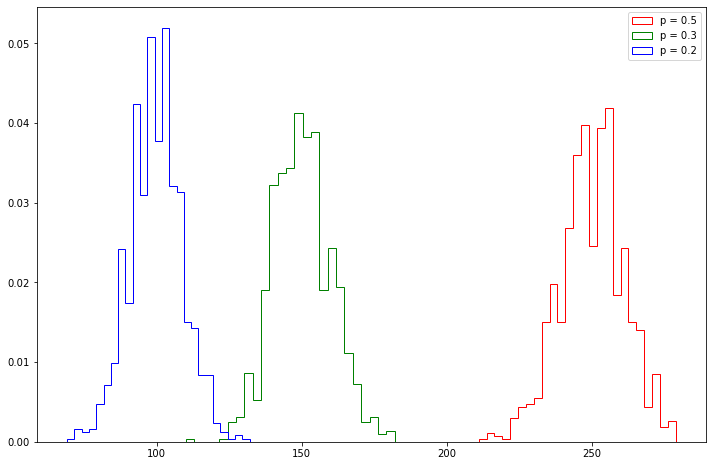
\includegraphics[width=0.9\linewidth,height=0.2\textheight,keepaspectratio]{Figure-15-01}
\end{figure}

\textbf{Exercise 15.6.5 (Computer Experiment)}. Write a function to
generate \(\text{nsim}\) observations from a Multivariate normal with
given mean \(\mu\) and covariance matrix \(\Sigma\).

\textbf{Solution}. Let's construct our samples based on samples of a
standard multivariate normal \(Z \sim N(0, I)\), by making
\(X = \mu + \Sigma^{1/2} Z\).

\begin{python}
import numpy as np

def multivariate_normal_observations(mu, sigma, nsim=1):
    mu_array = np.array(mu)
    sigma_array = np.array(sigma)
    
    assert len(mu_array.shape) == 1, "mu should be a vector"
    k = mu_array.shape[0]
    
    assert sigma_array.shape == (k, k), "sigma should be a square matrix with same length as mu"
    
    # Do the eigenvalue decomposition, then get U D^{1/2} as Sigma^{1/2}
    U, D, V = np.linalg.svd(sigma_array)
    sigma_sqrt = U @ np.diag(np.sqrt(D))
    
    # Let's write our own random normal generator for fun, rather than use np.random.normal
    # Strategy: Use Box-Muller to transform two random uniform variables in (0, 1) 
    # into two standard normals
    def random_normals(size):

        def box_muller(u1, u2):
            R = np.sqrt(-2 * np.log(u1))
            theta = 2 * np.pi * u2

            z0 = R * np.cos(theta)
            z1 = R * np.sin(theta)

            return z0, z1

        def normal_generator(uniform_generator):
            while True:
                z0, z1 = box_muller(next(uniform_generator), next(uniform_generator))
                yield z0
                yield z1

        def random_generator(batch_size):
            while True:
                for v in np.random.uniform(size=batch_size):
                    yield v

        result = np.empty(size)
        gen = normal_generator(random_generator(batch_size=min(size, 1024)))
        for i in range(size):
            result[i] = next(gen)

        return result

    def get_observation():
        z = random_normals(k)
        return mu_array + sigma_sqrt @ z
    
    return np.array([get_observation() for _ in range(nsim)])
\end{python}

\begin{python}
# Sample usage
import matplotlib.pyplot as plt

mu = [1, 3]
sigma = [[2, 1], [1, 2]]
obs = multivariate_normal_observations(mu, sigma, nsim=5000)

plt.figure(figsize=(12, 8))
plt.hexbin(obs[:, 0], obs[:, 1], cmap=plt.cm.Reds)
plt.show()
\end{python}

\begin{figure}[H]
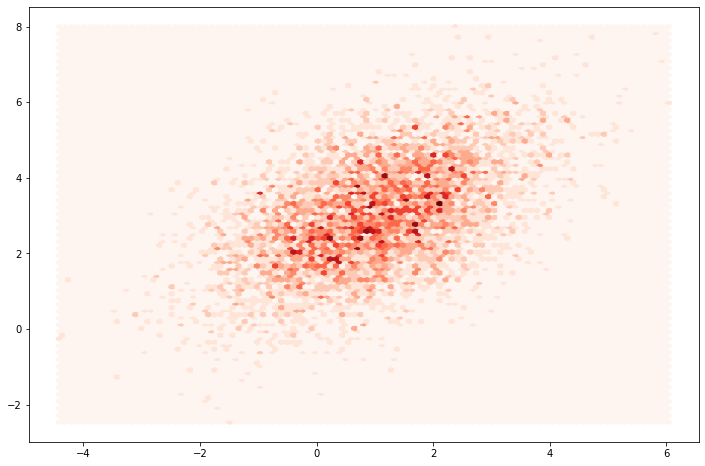
\includegraphics[width=0.9\linewidth,height=0.2\textheight,keepaspectratio]{Figure-15-02}
\end{figure}

\textbf{Exercise 15.6.6 (Computer Experiment)}. Generate 1000 random
vectors from a \(N(\mu, \Sigma)\) distribution where

\[ \mu = \begin{pmatrix} 3 \\ 8\end{pmatrix}
, \quad
\Sigma = \begin{pmatrix}
2 & 6 \\
6 & 2
\end{pmatrix}\]

Plot the simulation as a scatterplot. Find the distribution of
\(X_2 | X_1 = x_1\) using theorem 15.5. In particular, what is the
formula for \(\mathbb{E}(X_2 | X_1 = x_1)\)? Plot
\(\mathbb{E}(X_2 | X_1 = x_1)\) on your scatterplot. Find the
correlation \(\rho\) between \(X_1\) and \(X_2\). Compare this with the
sample correlations from your simulation. Find a 95\% confidence
interval for \(\rho\). Estimate the covariance matrix \(\Sigma\).

\textbf{Solution}.

The provided \(\Sigma\) matrix has negative eigenvalues. We will instead
use the following matrix:

\[ \Sigma = \begin{pmatrix} 6 & 2 \\ 2 & 6\end{pmatrix}\]

\begin{python}
# Generate 1000 vectors
mu = [3, 8]
sigma = [[2, 6], [6, 2]]
obs = multivariate_normal_observations(mu, sigma, nsim=1000)

# Using numpy to generate observations:
#obs = np.random.multivariate_normal(mu, sigma, size=1000)

# Using scipy to generate observations:
#obs = scipy.stats.multivariate_normal.rvs(mean=mu, cov=sigma, size=1000)

x, y = obs[:, 0], obs[:, 1]

# Plot scatterplot
plt.figure(figsize=(12, 8))
plt.scatter(x, y)
plt.show()
\end{python}

\begin{figure}[H]
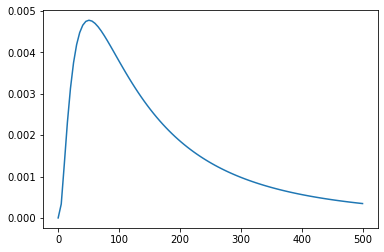
\includegraphics[width=0.9\linewidth,height=0.2\textheight,keepaspectratio]{Figure-12-04}
\end{figure}

From theorem 15.5,

\[ X_2 | X_1 = x_1 \sim N(\mu(x_1), \Sigma(x_1))\]

where

\begin{align}
\mu(x_1) &= \mu_2 + \Sigma_{21} \Sigma_{11}^{-1} (x_1 - \mu_1) \\
\Sigma(x_1) &= \Sigma_{22} - \Sigma_{21}\Sigma_{11}^{-1}\Sigma_{12}
\end{align}

Replacing the given values,

\begin{align}
\mu(x_1) &= 8 + 2 \cdot 6^{-1} (x_1 - 3) = \frac{1}{3} x_1 + \frac{22}{3}\\
\Sigma(x_1) &= 6 - 2 \cdot 6^{-1} \cdot 2 = \frac{16}{3}
\end{align}

\begin{python}
# Plot scatterplot + line
f = lambda x: x/3 + 22/3

plt.figure(figsize=(12, 8))
plt.scatter(x, y)
plt.plot([-6, 10], [f(-6), f(10)], color='red')
plt.show()
\end{python}

\begin{figure}[H]
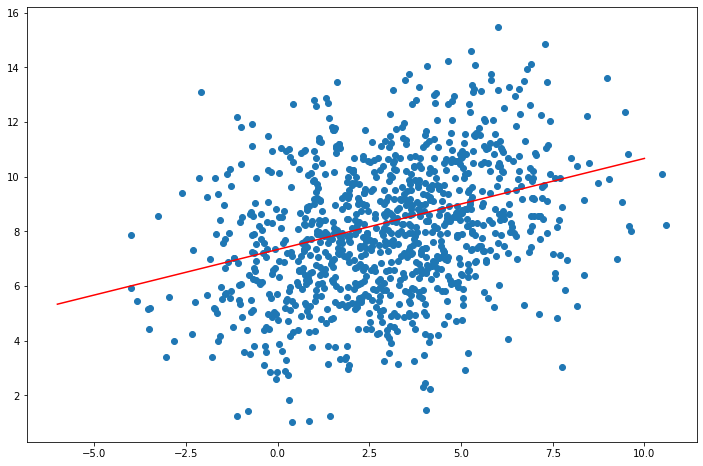
\includegraphics[width=0.9\linewidth,height=0.2\textheight,keepaspectratio]{Figure-15-04}
\end{figure}

The correlation \(\rho\) between \(X_1\) and \(X_2\) is:

\[ \rho = \frac{\text{Cov}(X_1, X_2)}{\sigma_{X_1} \sigma_{X_2}} = \frac{1}{3}\]

The estimated correlation \(\rho\) between \(X_1\) and \(X_2\) is:

\[ \hat{\rho} = \frac{\sum_i (X_{1i} - \overline{X}_1)(X_{2i} - \overline{X}_2)}{s_{X_1} s_{X_2}}\]

\begin{python}
rho_hat = np.corrcoef(x, y)[0, 1]
print("Estimated correlation: %.3f" % rho_hat)
\end{python}

\begin{console}
Estimated correlation: 0.327
\end{console}

We will use the provided process to estimate a confidence interval for
the correlation:

\textbf{Approximate Confidence Interval for the Correlation}

\begin{enumerate}[tightlist,label={\arabic*.}]
\item
  Compute
\end{enumerate}

\[\hat{\theta} = f(\hat{\rho}) = \frac{1}{2} \left( \log(1 + \hat{\rho}) - \log(1 - \hat{\rho})\right) \]

\begin{enumerate}[tightlist,label={\arabic*.},resume]
\item
  Compute the approximate standard error of \(\hat{\theta}\) which can
  be shown to be
\end{enumerate}

\[\hat{\text{se}}(\hat{\theta}) = \frac{1}{\sqrt{n - 3}} \]

\begin{enumerate}[tightlist,label={\arabic*.},resume]
\item
  An approximate \(1 - \alpha\) confidence interval for
  \(\theta = f(\rho)\) is
\end{enumerate}

\[(a, b) \equiv \left(\hat{\theta} - \frac{z_{\alpha/2}}{\sqrt{n - 3}}, \; \hat{\theta} + \frac{z_{\alpha/2}}{\sqrt{n - 3}} \right)\]

\begin{enumerate}[tightlist,label={\arabic*.},resume]
\item
  Apply the inverse transformation \(f^{-1}(z)\) to get a confidence
  interval for \(\rho\):
\end{enumerate}

\[ \left( \frac{e^{2a} - 1}{e^{2a} + 1}, \frac{e^{2b} - 1}{e^{2b} + 1} \right) \]

\begin{python}
from scipy.stats import norm

theta_hat = (np.log(1 + rho_hat) - np.log(1 - rho_hat)) / 2
se_theta_hat = 1 / np.sqrt(1000 - 3)
z = norm.ppf(0.975)
a, b = theta_hat - z * se_theta_hat, theta_hat + z * se_theta_hat
f_inv = lambda x: (np.exp(2*x) - 1) / (np.exp(2*x) + 1)
confidence_interval = (f_inv(a), f_inv(b))

print('95%% confidence interval: %.3f, %.3f' % confidence_interval)
\end{python}

\begin{console}
95\% confidence interval: 0.270, 0.381
\end{console}

The sample covariance matrix is:

\[ \hat{\Sigma} = \frac{1}{n} S = \frac{1}{n} \sum_{i=1}^n (X_i - \overline{X})(X_i - \overline{X})^T \]

\begin{python}
import numpy as np
mu_hat = np.array([x.mean(), y.mean()])
xx = np.concatenate((x.reshape(-1, 1), y.reshape(-1, 1)), axis=1)
sigma_hat = (xx - mu_hat).T @ (xx - mu_hat) / 1000

sigma_hat
\end{python}

\begin{console}
array([[6.17974344, 1.99813879],
       [1.99813879, 6.05196861]])
\end{console}

\textbf{Exercise 15.6.7 (Computer Experiment)}. Generate 100 random
vectors from a multivariate Normal with mean \((0, 2)^T\) and variance

\[ \begin{pmatrix}
1 & 3 \\
3 & 1
\end{pmatrix} \]

Find a 95\% confidence interval for the correlation \(\rho\). What is
the true value of \(\rho\)?

\textbf{Solution}.

The provided matrix, yet again, has negative eigenvalues. Let's instead
use:

\[\Sigma = \begin{pmatrix}
3 & 1 \\
1 & 3
\end{pmatrix}\]

\begin{python}
# Generate 100 vectors
n = 100
mu = [0, 2]
sigma = [[3, 1], [1, 3]]
obs = multivariate_normal_observations(mu, sigma, nsim=n)
x, y = obs[:, 0], obs[:, 1]
\end{python}

\begin{python}
# Find 95% confidence interval
from scipy.stats import norm

rho_hat = np.corrcoef(x, y)[0, 1]
theta_hat = (np.log(1 + rho_hat) - np.log(1 - rho_hat)) / 2
se_theta_hat = 1 / np.sqrt(n - 3)
z = norm.ppf(0.975)
a, b = theta_hat - z * se_theta_hat, theta_hat + z * se_theta_hat
f_inv = lambda x: (np.exp(2*x) - 1) / (np.exp(2*x) + 1)
confidence_interval = (f_inv(a), f_inv(b))

print('95%% confidence interval: %.3f, %.3f' % confidence_interval)
\end{python}


\begin{console}
95\% confidence interval: 0.054, 0.424
\end{console}

True value of \(\rho\):

\[ \rho = \frac{\text{Cov}(X_1, X_2)}{\sigma_{X_1} \sigma_{X_2}} = \frac{1}{3}\]


% Chapter 16
\section*{16. Inference about Independence}\label{inference-about-independence}
This chapter addresses two questions:
\begin{enumerate}[tightlist,label={\arabic*.}]
\item
  How do we test if two random variables are independent?
\item
  How do we estimate the strength of dependence between two random
  variables?
\end{enumerate}
Recall we write \(Y \ci Z\) to mean that \(Y\) and \(Z\) are
independent.
When \(Y\) and \(Z\) are not independent, we say they are
\textbf{dependent} or \textbf{associated} or \textbf{related}.
Note that dependence does not mean causation: - Smoking is related to
heart disease, and quitting smoking will reduce the chance of heart
disease. - Owning a TV is related to lower starvation, but giving a
starving person a TV does not make them not hungry.

\subsection*{16.1 Two Binary Variables}\label{two-binary-variables}
Suppose that both \(Y\) and \(Z\) are binary. Consider a data set
\((Y_{1}, Z_{1}), \dots, (Y_{n}, Z_{n})\). Represent the data as a two-by-two
table:
\[
\begin{array}{c|cc|c} 
      & Y = 0  & Y = 1 & \\
\hline
Z = 0 & X_{00} & X_{01} & X_{0\text{·}}\\
Z = 1 & X_{10} & X_{11} & X_{1\text{·}}\\
 \hline
      & X_{\text{·}0} & X_{\text{·}1} & n = X_{\text{··}}
\end{array}
\]
where \(X_{ij}\) represents the number of observations where
\((Z_{k}, Y_{k}) = (i, j)\). The dotted subscripts denote sums,
e.g.~\(X_{i\text{·}} = \sum_{j} X_{ij}\). Denote the corresponding
probabilities by:
\[
\begin{array}{c|cc|c} 
      & Y = 0  & Y = 1 & \\
\hline
Z = 0 & p_{00} & p_{01} & p_{0\text{·}}\\
Z = 1 & p_{10} & p_{11} & p_{1\text{·}}\\
 \hline
      & p_{\text{·}0} & p_{\text{·}1} & 1
\end{array}
\]
where \(p_{ij} = \PROB(Z = i, Y = j)\). Let
\(X = (X_{00}, X_{01}, X_{10}, X_{11})\) denote the vector of counts.
Then \(X \sim \text{Multinomial}(n, p)\) where
\(p = (p_{00}, p_{01}, p_{10}, p_{11})\).
The \textbf{odds ratio} is defined to be
\[
\psi = \frac{p_{00} p_{11}}{p_{01} p_{10}}
\]
The \textbf{log odds ratio} is defined to be
\[
\gamma = \log \psi
\]

\textbf{Theorem 16.2}. The following statements are equivalent:
\begin{enumerate}[tightlist,label={\arabic*.}]
\item
  \(Y \ci Z\)
\item
  \(\psi = 1\)
\item
  \(\gamma = 0\)
\item
  For \(i, j \in \{ 0, 1 \}\), \(p_{ij} = p_{i\text{·}} p_{\text{·}j}\)
\end{enumerate}
Now consider testing
\[
H_{0}: Y \ci Z
\quad \text{versus} \quad
H_{1}: \text{not} (Y \ci Z)
\]
First consider the likelihood ratio test. Under \(H_{1}\),
\(X \sim \text{Multinomial}(n, p)\) and the MLE is \(\hat{p} = X / n\).
Under \(H_{0}\), again \(X \sim \text{Multinomial}(n, p)\) but \(p\) is
subjected to the constraint \(p_{ij} = p_{i.} p_{.j}\). This leads to
the following test.

\textbf{Theorem 16.3 (Likelihood Ratio Test for Independence in a 2-by-2
table)}. Let
\[
T = 2 \sum_{i=0}^{1} \sum_{j=0}^{1} X_{ij} \log \left( \frac{X_{ij} X_{\text{··}}}{X_{i\text{·}} X_{\text{·}j}} \right)
\]
Under \(H_{0}\), \(T \leadsto \chi_{1}^{2}\). Thus, an approximate level
\(\alpha\) test is obtained by rejecting \(H_{0}\) when
\(T > \chi_{1, \alpha}^{2}\).

\textbf{Theorem 16.4 (Pearson's \(\chi^{2}\) test for Independence in a
2-by-2 table)}. Let
\[
U = \sum_{i=0}^{1} \sum_{j=0}^{1} \frac{(X_{ij} - E_{ij})^{2}}{E_{ij}}
\]
where
\[
E_{ij} = \frac{X_{i\text{·}} X_{\text{·}j}}{n}
\]
Under \(H_{0}\), \(U \leadsto \chi_{1}^{2}\). Thus, an approximate level
\(\alpha\) test is obtained by rejecting \(H_{0}\) when
\(U > \chi_{1, \alpha}^{2}\).
Here is the intuition for the Pearson test: Under \(H_{0}\),
\(p_{ij} = p_{i\text{·}} p_{\text{·}j}\), so the MLE of \(p_{ij}\) is
\(\hat{p}_{ij} = \hat{p}_{i\text{·}} \hat{p}_{\text{·}j} = \frac{X_{i\text{·}}}{n} \frac{X_{\text{·}j}}{n}\).
Thus, the expected number of observations in the \((i, j)\) cell is
\(E_{ij} = n \hat{p}_{ij} = \frac{X_{i\text{·}} X_{\text{·}j}}{n}\). The
statistic \(U\) compares the observed and expected counts.

\textbf{Theorem 16.6}. The MLEs of \(\psi\) and \(\gamma\) are
\[
\hat{\psi} = \frac{X_{00} X_{11}}{X_{01} X_{10}}
, \quad
\hat{\gamma} = \log \hat{\psi}
\]
The asymptotic standard errors (computed from the delta method) are
\begin{align*}
\widehat{\SE}(\hat{\psi}) &= \sqrt{\frac{1}{X_{00}} + \frac{1}{X_{01}} + \frac{1}{X_{10}} + \frac{1}{X_{11}}}\\
\widehat{\SE}(\hat{\gamma}) &= \hat{\psi} \widehat{\SE}(\hat{\gamma})
\end{align*}
Yet another test of independence is the Wald test for \(\gamma = 0\)
given by \(W = (\hat{\gamma} - 0) / \widehat{\SE}(\hat{\gamma})\).
A \(1 - \alpha\) confidence interval for \(\gamma\) is
\(\hat{\gamma} \pm z_{\alpha/2} \widehat{\SE}(\hat{\gamma})\).
A \(1 - \alpha\) confidence interval for \(\psi\) can be obtained in two
ways. First, we could use
\(\hat{\psi} \pm z_{\alpha/2} \widehat{\SE}(\hat{\psi})\). Second,
since \(\psi = e^{\gamma}\) we could use
\(\exp \{\hat{\gamma} \pm z_{\alpha/2} \widehat{\SE}(\hat{\gamma})\}\).
This second method is usually more accurate.

\subsection*{16.2 Interpreting the Odds
Ratios}\label{interpreting-the-odds-ratios}
Suppose event \(A\) has probability \(\PROB(A)\). The odds of \(A\)
are defined as
\[
\text{odds}(A) = \frac{\PROB(A)}{1 - \PROB(A)}
\]
It follows that
\[
\PROB(A) = \frac{\text{odds}(A)}{1 + \text{odds}(A)}
\]
Let \(E\) be the event that someone is exposed to something (smoking,
radiation, etc) and let \(D\) be the event that they get a disease. The
odds of getting the disease given exposure are:
\[
\text{odds}(D | E) = \frac{\PROB(D | E)}{1 - \PROB(D | E)}
\]
and the odds of getting the disease given non-exposure are:
\[
\text{odds}(D | E^{c}) = \frac{\PROB(D | E^{c})}{1 - \PROB(D | E^{c})}
\]
The \textbf{odds ratio} is defined to be
\[
\psi = \frac{\text{odds}(D | E)}{\text{odds}(D | E^{c})}
\]
If \(\psi = 1\) then the disease probability is the same for exposed and
unexposed; this implies these events are independent. Recall that the
log-odds ratio is defined as \(\gamma = \log \psi\). Independence
corresponds to \(\gamma = 0\).
Consider this table of probabilities:
\[
\begin{array}{c|cc|c} 
      & D^{c}    & D      & \\
\hline
E^{c}   & p_{00} & p_{01} & p_{0\text{·}}\\
E     & p_{10} & p_{11} & p_{1\text{·}}\\
 \hline
      & p_{\text{·}0} & p_{\text{·}1} & 1
\end{array}
\]
Denote the data by
\[
\begin{array}{c|cc|c} 
      & D^{c}    & D      & \\
\hline
E^{c}   & X_{00} & X_{01} & X_{0\text{·}}\\
E     & X_{10} & X_{11} & X_{1\text{·}}\\
 \hline
      & X_{\text{·}0} & X_{\text{·}1} & X_{\text{··}}
\end{array}
\]
Now
\[
\PROB(D | E) = \frac{p_{11}}{p_{10} + p_{11}}
\quad \text{and} \quad
\PROB(D | E^{c}) = \frac{p_{01}}{p_{00} + p_{01}}
\]
and so
\[
\text{odds}(D | E) = \frac{p_{11}}{p_{10}}
\quad \text{and} \quad
\text{odds}(D | E^{c}) = \frac{p_{01}}{p_{00}}
\]
and therefore
\[
\psi = \frac{p_{11}p_{00}}{p_{01}p_{10}}
\]
To estimate the parameters, we have to consider how the data were
collected. There are three methods.
\textbf{Multinomial Sampling}. We draw a sample from the population and, for each sample, record their exposure and disease status. In this case, 
\(X = (X_{00}, X_{01}, X_{10}, X_{11}) \sim \text{Multinomial}(n, p)\). 
We then estimates the probabilities in the table by 
\(\hat{p}_{ij} = X_{ij} / n\) and
\[
\hat{\psi} = \frac{\hat{p}_{11} \hat{p}_{00}}{\hat{p}_{01} \hat{p}_{10}} = \frac{X_{11} X_{00}}{X_{01} X_{10}}
\]
\textbf{Prospective Sampling (Cohort Sampling)}. We get some exposed and
unexposed people and count the number with disease within each group.
Thus,
\[
X_{01} \sim \text{Binomial}(X_{0\text{·}}, \PROB(D | E^{c}))
\quad \text{and} \quad
X_{11} \sim \text{Binomial}(X_{1\text{·}}, \PROB(D | E))
\]
In this case we should write small letters
\(x_{0\text{·}},  x_{1\text{·}}\) instead of capital letters $
X_{0\placeholder}, X_{1\placeholder}$ since they are fixed and not
random, but we'll keep using capital letters for notational simplicity.
We can estimate \(\PROB(D | E))\) and \(\PROB(D | E^{c})\) but
we cannot estimate all probabilities in the table. Still, we can
estimate \(\psi\). Now:
\[
\hat{\PROB}(D | E) = \frac{X_{11}}{X_{1\text{·}}}
\quad \text{and} \quad
\hat{\PROB}(D | E^{c}) = \frac{X_{01}}{X_{0\text{·}}}
\]
Thus,
\[
\hat{\psi} = \frac{X_{11} X_{00}}{X_{01} X_{10}}
\]
as before.
\textbf{Case-Control (Retrospective Sampling)}. Here we get some
diseased and non-diseased people and we observe how many are exposed.
This is much more efficient if the disease is rare. Hence,
\[
X_{10} \sim \text{Binomial}(X_{\text{·}0}, \PROB(E | D^{c}))
\quad \text{and} \quad
X_{11} \sim \text{Binomial}(X_{\text{·}1}, \PROB(E | D))
\]
From this data we can estimate \(\PROB(E | D)\) and
\(\PROB(E | D^{c})\). Surprisingly, we can still estimate \(\psi\).
To understand why, note that
\[
\PROB(E | D) = \frac{p_{11}}{p_{01} + p_{11}},
\quad 1 - \PROB(E | D) = \frac{p_{01}}{p_{01} + p_{11}},
\quad \text{odds}(E | D) = \frac{p_{11}}{p_{01}}
\]
By a similar argument,
\[
\text{odds}(E | D^{c}) = \frac{p_{10}}{p_{00}}
\]
Hence,
\[
\frac{\text{odds}(E | D)}{\text{odds}(E | D^{c})} = \frac{p_{11} p_{00}}{p_{01} p_{10}} = \psi
\]
Therefore,
\[
\hat{\psi} = \frac{X_{11} X_{00}}{X_{01} X_{10}}
\]
In all three methods, the estimate of \(\psi\) turns out to be the same.
It is tempting to try to estimate
\(\PROB(D | E) - \PROB(D | E^{c})\). In a case-control design,
this quantity is not estimable. To see this, we apply Bayes' Theorem to
get
\[
\PROB(D | E) - \PROB(D | E^{c}) = \frac{\PROB(E | D) \PROB(D))}{\PROB(E)} - \frac{\PROB(E^{c} | D) \PROB(D)}{\PROB(E^{c})}
\]
Because of the way we obtained the data, \(\PROB(D)\) is not
estimable from the data.
However, we can estimate
\(\xi = \PROB(D | E) / \PROB(D | E^{c})\), which is called the
\textbf{relative risk}, under the \textbf{rare disease assumption}.

\textbf{Theorem 16.9}. Let
\(\xi = \PROB(D | E) / \PROB(D | E^{c})\). Then
\[
\frac{\psi}{\xi} \rightarrow 1
\]
as \(\PROB(D) \rightarrow 0\).
Thus, under the rare disease assumption, the relative risk is
approximately the same as the odds ratio, which we can estimate.
In a randomized experiment, we can interpret a strong association, that
is \(\psi \neq 1\), as a causal relationship. In an observational
(non-randomized) study, the association can be due to other unobserved
\textbf{confounding} variables. We'll discuss causation in more detail
later.

\subsection*{16.3 Two Discrete
Variables}\label{two-discrete-variables}
Now suppose that \(Y \in \{ 1, \dots, I \}\) and
\(Z \in \{ 1, \dots, J \}\) are two discrete variables. The data can be
represented by an \(I \times J\) table of contents:
    \[
\begin{array}{c|cccccc|c} 
       & Y = 1  & Y = 2  & \cdots & Y = j & \cdots & Y = J   & \\
\hline
Z = 1 & X_{11}  & X_{12} & \cdots & X_{1j} & \cdots & X_{1J} & X_{1\text{·}}\\
Z = 2 & X_{21}  & X_{22} & \cdots & X_{2j} & \cdots & X_{2J} & X_{2\text{·}}\\
\vdots & \vdots & \vdots & \vdots & \vdots & \vdots & \vdots & \vdots\\
Z = i & X_{i1}  & X_{i2} & \cdots & X_{ij} & \cdots & X_{iJ} & X_{i\text{·}}\\
\vdots & \vdots & \vdots & \vdots & \vdots & \vdots & \vdots & \vdots\\
Z = I & X_{I1}  & X_{I2} & \cdots & X_{Ij} & \cdots & X_{IJ} & X_{I\text{·}}\\
 \hline
      & X_{\text{·}1} & X_{\text{·}1} & \cdots & X_{\text{·}j} & \cdots & X_{\text{·}J} & n
\end{array}
\]
Consider testing
\[
H_{0}: Y \ci Z
\quad \text{versus} \quad
H_{1}: \text{not } H_{0}
\]

\textbf{Theorem 16.10}. Let
\[
T = 2 \sum_{i=1}^I \sum_{j=1}^J X_{ij} \log \left( \frac{X_{ij} X_{\text{··}}}{X_{i\text{·}} X_{\text{·}j}} \right)
\]
The limiting distribution of \(T\) under the null hypothesis of
independence is \(\chi^{2}_\nu\) where \(\nu = (I - 1)(J - 1)\).
Pearson's \(\chi^{2}\) test statistic is
\[
U = \sum_{i=1}^I \sum_{j=1}^J \frac{(n_{ij} - E_{ij})^{2}}{E_{ij}}
\]
Asymptotically, under \(H_{0}\), \(U\) has a \(\chi^{2}_\nu\) distribution
where \(\nu = (I - 1)(J - 1)\).
There are a variety of ways to quantify the strength of dependence
between two discrete variables \(Y\) and \(Z\). Most of them are not
very intuitive. The one we shall use is not standard but is more
interpretable.
We define
\[
\delta(Y, Z) = \max_{A, B} \Big|\; \PROB_{Y, Z}(Y \in A, Z \in B) - \PROB_Y(Y \in A)\PROB_Z(Z \in B) \;\Big|
\]
where the maximum is over all pairs of events \(A\) and \(B\).
\emph{Note: the original version on the book contains a typo; it is
originally stated as}
\[
\delta(Y, Z) = \max_{A, B} \Big|\; \PROB_{Y, Z}(Y \in A, Z \in B) - \PROB_Y(Y \in A) - \PROB_Z(Z \in B) \;\Big|
\]
\emph{For more context, this is a specific case of the ``total variation
distance'' \(\delta(P_{1}, P_{2})\) between the probability metrics
\(P_{1}(Y, Z) = \PROB_{Y, Z}(Y \in A, Z \in B)\) and
\(P_{2}(Y, Z) = \PROB_Y(Y \in A)\PROB_Z(Z \in B)\).}

\textbf{Theorem 16.12}. Properties of \(\delta(Y, Z)\):
\begin{enumerate}[tightlist,label={\arabic*.}]
\item
  \(0 \leq \delta(Y, Z) \leq 1\)
\item
  \(\delta(Y, Z) = 0\) if and only if \(Y \ci Z\)
\item
  The following identity holds:
\end{enumerate}
\[
\delta(X, Y) = \frac{1}{2} \sum_{i=1}^I \sum_{j=1}^J \Big|\; p_{ij} - p_{i\text{·}} p_{\text{·}j} \;\Big|
\]
\begin{enumerate}[tightlist,label={\arabic*.},resume]
\item
  The MLE of \(\delta\) is
\end{enumerate}
\[
\hat{\delta}(X, Y) = \frac{1}{2} \sum_{i=1}^I \sum_{j=1}^J \Big|\; \hat{p}_{ij} - \hat{p}_{i\text{·}} \hat{p}_{\text{·}j} \;\Big|
\]
where
\[
\hat{p}_{ij} = \frac{X_{ij}}{n},
\quad \hat{p}_{i\text{·}} = \frac{X_{i\text{·}}}{n},
\quad \hat{p}_{\text{·}j} = \frac{X_{\text{·}j}}{n}
\]
The interpretation of \(\delta\) is this: if one person makes
probability statements assuming independence and another person makes
probability statements without assuming independence, their probability
statements may differ by as much as \(\delta\). Here is a suggested scale
for interpreting \(\delta\):
\begin{table}[H]
\centering
\begin{tabular}{@{}ll@{}}
\toprule
range & interpretation \\
\midrule
0 to 0.01 & negligible association \\
0.01 to 0.05 & non-negligible association \\
0.05 to 0.1 & substantial association \\
over 0.1 & very strong association \\
\bottomrule
\end{tabular}
\end{table}
A confidence interval for \(\delta\) can be obtained by bootstrapping.
The steps are:
\begin{enumerate}[tightlist,label={\arabic*.}]
\item
  Draw \(X^{*} \sim \text{Multinomial}(n, \hat{p})\);
\item
  Compute \(\hat{p}_{ij}, \hat{p}_{i\text{·}}, \hat{p}_{\text{·}j}\);
\item
  Compute \(\delta^{*}\);
\item
  Repeat.
\end{enumerate}
Now we use any of the methods we learned earlier for constructing
bootstrap confidence intervals. However, we should not use a Wald
interval in this case. The reason is that if \(Y\) and \(Z\) are
independent then \(\delta = 0\) and we are on the boundary of the
parameter space. In this case, the Wald method is not valid.

\subsection*{16.4 Two Continuous
Variables}\label{two-continuous-variables}
Now suppose that \(Y\) and \(Z\) are both continuous. If we assume that
the joint distribution of \(Y\) and \(Z\) is bivariate Normal, then we
measure the dependence between \(Y\) and \(Z\) by means of the
correlation coefficient \(\rho\). Tests, estimates, and confidence
intervals for \(\rho\) in the Normal case are given in the previous
chapter. If we do not assume normality, then we need a nonparametric
method for asserting dependence.
Recall that the correlation is
\[
\rho = \frac{\EXP((X_{1} - \mu_{1})(X_{2} - \mu_{2}))}{\sigma_{1} \sigma_{2}}
\]
A nonparametric estimator of \(\rho\) is the plug-in estimator which is:
\[
\hat{\rho} = \frac{\sum_{i=1}^{n} (X_{1i} - \bar{X}_{1})(X_{2i} - \bar{X}_{2})}{\sqrt{\sum_{i=1}^{n} (X_{1i} - \bar{X}_{1})^{2} \sum_{i=1}^{n} (X_{2i} - \bar{X}_{2})^{2}}}
\]
which is just the sample correlation. A confidence interval can be
constructed using the bootstrap. A test for \(\rho = 0\) can be based on
the Wald test using the bootstrap to estimate the standard error.
The plug-in approach is useful for large samples. For small samples, we
measure the correlation using the \textbf{Spearman rank correlation
coefficient} \(\hat{\rho}_S\). We simply replace the data by their
ranks, ranking each variable separately, then compute the correlation
coefficient of the ranks.
To test the null hypothesis that \(\rho_S = 0\), we need the
distribution of \(\hat{\rho}_S\) under the null hypothesis. This can be
obtained by simulation. We fix the ranks of the first variable as
\(1, 2, \dots, n\). The ranks of the second variable are chosen at
random from the set of \(n!\) possible orderings, then we compute the
correlation. This is repeated many times, and the resulting distribution
\(\PROB_{0}\) is the null distribution of \(\hat{\rho}_S\). The
p-value for the test is \(\PROB_{0}(|R| > |\hat{\rho}_S|)\) where
\(R\) is drawn from the null distribution \(\PROB_{0}\).

\subsection*{16.5 One Continuous Variable and One
Discrete}\label{one-continuous-variable-and-one-discrete}
Suppose that \(Y \in \{ 1, \dots, I \}\) is discrete and \(Z\) is
continuous. Let \(F_{i}(z) = \PROB(Z \leq z | Y = i)\) denote the CDF
of \(Z\) conditional on \(Y = i\).

\textbf{Theorem 16.15}. When \(Y \in \{ 1, 2, \dots, I \}\) is discrete
and \(Z\) is continuous, then \(Y \ci Z\) if and only if
\(F_{1} = F_{2} = \dots = F_I\).
It follows that to test for independence, we need to test
\[
H_{0}: F_{1} = \dots = F_I
\quad \text{versus} \quad
H_{1}: \text{not } H_{0}
\]
For simplicity, we consider the case where \(I = 2\). To test the null
hypothesis that \(F_{1} = F_{2}\) we will use the \textbf{two sample
Kolmogorov-Smirnov test}.
Let \(n_{k}\) denote the number of observations for which \(Y_{i} = k\). Let
\[
\hat{F}_{k}(z) = \frac{1}{n_{k}} \sum_{i=1}^{n} I(Z_{i} \leq z) I(Y_{i} = k)
\]
denote the empirical distribution function of \(Z\) given \(Y = k\).
Define the test statistic
\[
D = \sup_x | \hat{F}_{1}(x) - \hat{F}_{2}(x) |
\]

\textbf{Theorem 16.16}. Let
\[
H(t) = 1 - 2 \sum_{j=1}^{\infty} (-1)^{j-1} e^{-2j^{2}t^{2}}
\]
Under the null hypothesis that \(F_{1} = F_{2}\),
\[
\lim_{n \rightarrow \infty} \PROB \left( \sqrt{\frac{n_{1} n_{2}}{n_{1} + n_{2}}} D \leq t \right) = H(t)
\]
It follows from the Theorem than an approximate level \(\alpha\) test is
obtained by rejecting \(H_{0}\) when
\[
\sqrt{\frac{n_{1} n_{2}}{n_{1} + n_{2}}} D > H^{-1}(1 - \alpha)
\]

\subsection*{16.7 Exercises}

\textbf{Exercise 16.7.1}. Prove Theorem 16.2.
The following statements are equivalent:
\begin{enumerate}[tightlist,label={\arabic*.}]
\item
  \(Y \ci Z\)
\item
  \(\psi = 1\)
\item
  \(\gamma = 0\)
\item
  For \(i, j \in \{ 0, 1 \}\), \(p_{ij} = p_{i\text{·}} p_{\text{·}j}\)
\end{enumerate}

\textbf{Solution}.
\(Y\) and \(Z\) are independent if and only if
\(\PROB(Y = j | Z = i) = \PROB(Y = j) \PROB(Z = i)\) for
all \(i\) and \(j\), so (1) and (4) are equivalent.
\(\gamma = \log \psi\), so (2) and (3) are equivalent.
Finally,
\begin{align*}
&\psi = 1\\
&\Leftrightarrow \frac{\text{odds}(Y | Z = 1)}{\text{odds}(Y | Z = 0)} = 1 \\
&\Leftrightarrow \text{odds}(Y | Z = 1) = \text{odds}(Y | Z = 0) \\
&\Leftrightarrow \PROB(Y | Z = 1) = \PROB(Y | Z = 0) \\
&\Leftrightarrow Y \ci Z
\end{align*}
so (1) and (2) are equivalent.
Therefore, all statements are equivalent.

\textbf{Exercise 16.7.2}. Prove Theorem 16.3.
Let
\[
T = 2 \sum_{i=0}^{1} \sum_{j=0}^{1} X_{ij} \log \left( \frac{X_{ij} X_{\text{··}}}{X_{i\text{·}} X_{\text{·}j}} \right)
\]
Under \(H_{0}\), \(T \leadsto \chi_{1}^{2}\). Thus, an approximate level
\(\alpha\) test is obtained by rejecting \(H_{0}\) when
\(T > \chi_{1, \alpha}^{2}\).

\textbf{Solution}. Let
\(E_{ij} = \frac{X_{i\text{·}} X_{\text{·}j}}{X_\text{··}}\). We can
rewrite the test statistic as
\[
T = 2 \sum_{i, j} X_{ij} \log \frac{X_{ij}}{E_{ij}}
\]
The interpretation of \(E_{ij}\) is that it is the expected count in
cell \((i, j)\) under \(H_{0}\):
\begin{align*}
\EXP_{H_{0}}(Y = i, Z = j) &= n \PROB_{H_{0}}(Y = i, Z = j) \\
&= n \PROB(Y = i) \PROB(Z = j) \\
&= n \hat{p}_{i\text{·}} \hat{p}_{\text{·}j} \\
&= X_{\text{··}} \frac{X_{i\text{·}}}{X_{\text{··}}} \frac{X_{\text{·}j}}{X_{\text{··}}} \\
&= E_{ij}
\end{align*}
Now, the result will follow by applying the log-likelihood test between
\(H_{0}\) and \(H_{1}\). The test statistic is:
\[
2 \log \frac{\mathcal{L}(\tilde{p} | X)}{\mathcal{L}(\hat{p} | X)} 
= 2 \log \frac{\prod_{i, j} \tilde{p}_{ij}^{X_{ij}}}{\prod_{i, j} \hat{p}_{ij}^{X_{ij}}}
\]
where \(\tilde{p}\) is the MLE under \(H_{1}\) and \(\hat{p}\) is the MLE
under \(H_{0}\). But we have:
\[
\tilde{p}_{ij} = \frac{X_{ij}}{n}
\quad \text{and} \quad
\hat{p}_{ij} = \frac{E_{ij}}{n}
\]
Substituting the MLEs on the log-likelihood ratio, we get
\[
2 \log \frac{\mathcal{L}(\tilde{p} | X)}{\mathcal{L}(\hat{p} | X)} 
= 2 \log \prod_{i, j} \left( \frac{X_{ij}}{E_{ij}} \right)^{X_{ij}}
= 2 \sum_{i, j} X_{ij} \log \frac{X_{ij}}{E_{ij}}
\]
which is the desired result.
\emph{Reference: ``G-test.'' Wikipedia: The Free Encyclopedia. Wikimedia
Foundation, Inc.~22 July 2004. Web. 17 Mar.~2020,
en.wikipedia.org/w/index.php?title=G-test\&oldid=914538756}

\textbf{Exercise 16.7.3}. Prove Theorem 16.9.
Let \(\xi = \PROB(D | E) / \PROB(D | E^{c})\). Then
\[
\frac{\psi}{\xi} \rightarrow 1
\]
as \(\PROB(D) \rightarrow 0\).

\textbf{Solution}. We have:
\[
\PROB(D | E) = \frac{\PROB(D \land E)}{\PROB(E)} = \frac{p_{11}}{p_{01} + p_{11}}
\quad
\PROB(D | E^{c}) = \frac{\PROB(D \land E^{c})}{\PROB(E^{c})} = \frac{p_{10}}{p_{00} + p_{10}}
\]
and so
\[
\xi = \frac{\PROB(D | E)}{\PROB(D | E^{c})}
= \frac{p_{11} (p_{00} + p_{10})}{p_{10} (p_{01} + p_{11})}
\]
Since
\[
\psi = \frac{p_{11}p_{00}}{p_{01}p_{10}}
\]
we have:
\[
\frac{\psi}{\xi} = \frac{p_{11}p_{00}}{p_{01}p_{10}} \frac{p_{10} (p_{01} + p_{11})}{p_{11} (p_{00} + p_{10})} 
= \frac{p_{00}}{p_{01}} \frac{p_{\text{·}1}}{p_{\text{·}0}}
\]
As \(\PROB(D) = p_{10} + p_{11} \rightarrow 0\) and the
probabilites are non-negative, \(p_{10} \rightarrow 0\),
\(p_{11} \rightarrow 0\), so
\[
\frac{\psi}{\xi} \rightarrow  \frac{p_{00}}{p_{01}} \frac{p_{01}}{p_{00}} = 1
\]

\textbf{Exercise 16.7.4}. Prove equation (16.14).
\[
\delta(X, Y) = \max_{A, B} \Big|\; \PROB_{X, Y}(X \in A, Y \in B) - \PROB_X(X \in A) \PROB_Y(Y \in B) \;\Big|
\]
is equivalent to
\[
\delta(X, Y) = \frac{1}{2} \sum_{i=1}^I \sum_{j=1}^J \Big|\; p_{ij} - p_{i\text{·}} p_{\text{·}j} \;\Big|
\]

\textbf{Solution}.
As noted when the definition was introduced, this definition of
\(\delta(X, Y)\) is a particular case of the total variation distance
between metrics \(P_{1}(X, Y) = \PROB_{X, Y}(X \in A, Y \in B)\) and
\(P_{2}(X, Y) = \PROB_X(X \in A) \PROB_Y(Y \in B)\), where
\[
\delta(P, Q) = \sup_{A \in \mathcal{F}} |P(A) - Q(A)|
\]
and \(P, Q\) are two probability measures on a sigma-algebra
\(\mathcal{F}\) of subsets from the sample space \(\Omega\).
(Note that \(P_{1}(X = i, Y = j) = p_{ij}\) and
\(P_{2}(X = i, Y = j) =  p_{i\text{·}} p_{\text{·}j}\)).
It is a known property of the total variation distance in countable
spaces that
\[
\delta(P, Q) = \max_{A \in \mathcal{F}} |P(A) - Q(A)| = \frac{1}{2} \Vert P - Q \Vert_{1} = \frac{1}{2} \sum_{\omega \in \Omega} \vert P(\omega) - Q(\omega) \vert
\]
Demonstrate it, following the steps in the reference below.
Let \(\mathcal{F}^+ \subset \mathcal{F}\) be the set of states
\(\omega\) such that \(P(\omega) \geq Q(\omega)\), and let
\(\mathcal{F}^- = \mathcal{F} - S^+\) be the set of states \(\omega\)
such that \(P(\omega) < Q(\omega)\). We have:
\[
\max_{A \in \mathcal{F}} P(A) - Q(A) = P(\mathcal{F}^+) - Q(\mathcal{F}^+)
\]
and
\[
\max_{A \in \mathcal{F}} Q(A) - P(A) = Q(\mathcal{F}^-) - P(\mathcal{F}^-)
\]
But since \(P(\Omega) = Q(\Omega) = 1\), we have
\[
P(\mathcal{F}^+) + P(\mathcal{F}^-) = Q(\mathcal{F}^+) + Q(\mathcal{F}^-) = 1
\]
which implies that
\[
P(\mathcal{F}^+) - Q(\mathcal{F}^+) = Q(\mathcal{F}^-) - P(\mathcal{F}^-)
\]
hence
\[
\max_{A \in \mathcal{F}} P(A) - Q(A) = \vert P(\mathcal{F}^+) - Q(\mathcal{F}^+) \vert = \vert Q(\mathcal{F}^-) - P(\mathcal{F}^-) \vert
\]
Finally, since
\[
\vert P(\mathcal{F}^+) - Q(\mathcal{F}^+) \vert + \vert Q(\mathcal{F}^-) - P(\mathcal{F}^-) \vert = \sum_{\omega \in \Omega} | P(\omega) - Q(\omega) | = \Vert P - Q \Vert_{1}
\]
we have that
\[
\max_{A \in \mathcal{F}} |P(A) - Q(A)| = \frac{1}{2} \Vert P - Q \Vert_{1}
\]
which completes the proof.
\emph{Reference: Upfal, E., and M. Mitzenmacher. ``Probability and
computing.'' (2005). Lemma 11.1, pg. 272-273.}

\textbf{Exercise 16.7.5}. The New York Times (January 8, 2003, page A12)
reported the following data on death sentencing and rance, from a study
in Maryland:
\begin{table}[H]
\centering
\begin{tabular}{@{}lll@{}}
\toprule
& Death Sentence & No Death Sentence \\
\midrule
Black Victim & 14 & 641 \\
White Victim & 62 & 594 \\
\bottomrule
\end{tabular}
\end{table}
Analyse the data using the tools from this Chapter. Interpret the
results. Explain why, based only on this information, you cannot make
causal conclusions. (The authors of the study did use much more
information in their full report).

\textbf{Solution}.
The statistic for the log-likelihood test for independence is is:
\[
T = 2 \sum_{i, j} X_{ij} \log \frac{X_{ij} X_{\text{··}}}{X_{i\text{·}} X_{\text{·}j}}
\]
The statistic for Pearson's \(\chi^{2}\) test is:
\[
U = \sum_{i, j} \frac{(X_{ij} - E_{ij})^{2}}{E_{ij}}
\]

\begin{python}
import numpy as np
X_ij = np.array([[14, 641], [62, 594]])
\end{python}

\begin{python}
X_idot = X_ij.sum(axis = 1).reshape(2, 1)
X_dotj = X_ij.sum(axis = 0).reshape(1, 2)
n = X_ij.sum()
E_ij = X_idot @ X_dotj / n
# Log-likelihood test statistic
T = 2 * (X_ij * np.log(X_ij / E_ij)).sum()
# Pearson's \chi^{2} test statistic
U = ((X_ij - E_ij)**2 / E_ij).sum()
\end{python}

\begin{python}
from scipy.stats import chi2
p_value_log_likelihood = 1 - chi2.cdf(T, 1)
p_value_pearson = 1 - chi2.cdf(U, 1)
print('T test statistic: \t\t%.3f'% T)
print('Pearson chi^{2} statistic: \t%.3f'% U)
print('p-value log likelihood:\t\t %.3f' % p_value_log_likelihood)
print('p-value Pearson: \t\t %.3f' % p_value_pearson)
\end{python}
\begin{console}
T test statistic:               34.534
Pearson chi^{2} statistic:        32.104
p-value log likelihood:          0.000
p-value Pearson:                 0.000
\end{console}
Both tests indicate that these variables are correlated. Note that this
is not sufficient information, in itself, to imply causation.

\begin{python}
from itertools import product
p = X_ij / n
p_idot = X_idot / n
p_dotj = X_dotj / n
delta = sum([abs(p[i, j] - p_idot[i, :] * p_dotj[:, j]) 
            for (i, j) in product(range(2), range(2))]) / 2
print('delta(X, Y): %.3f' % delta)
\end{python}
\begin{console}
delta(X, Y): 0.037
\end{console}
\(\delta(X, Y)\) is between 0.01 and 0.05, suggesting a non-negligible
association.

\textbf{Exercise 16.7.6}. Analyse the data on the variables Age and
Financial Status from:
\url{http://lib.stat.cmu.edu/DASL/Datafiles/montanadat.html}

\textbf{Solution}.

\begin{python}
import pandas as pd
data = pd.read_csv('data/montana.csv')
# Select wanted columns and remove missing data
data = data[['AGE', 'FIN']].replace('*', np.nan).dropna().astype(int)
\end{python}

\begin{python}
# Count occurrences in each cell
X_ij = np.zeros((3, 3)).astype(int)
for index, row in data.iterrows():
     X_ij[row['AGE'] - 1, row['FIN'] - 1] += 1
           
X_ij
\end{python}
\begin{console}
array([[21, 16, 34],
       [17, 23, 26],
       [22, 37, 11]])
\end{console}

\begin{python}
X_idot = X_ij.sum(axis = 1).reshape(3, 1)
X_dotj = X_ij.sum(axis = 0).reshape(1, 3)
n = X_ij.sum()
E_ij = X_idot @ X_dotj / n
# Log-likelihood test statistic
T = 2 * (X_ij * np.log(X_ij / E_ij)).sum()
# Pearson's \chi^{2} test statistic
U = ((X_ij - E_ij)**2 / E_ij).sum()
\end{python}

\begin{python}
from scipy.stats import chi2
p_value_log_likelihood = 1 - chi2.cdf(T, 4)
p_value_pearson = 1 - chi2.cdf(U, 4)
print('T test statistic: \t\t%.3f'% T)
print('Pearson chi^{2} statistic: \t%.3f'% U)
print('p-value log likelihood:\t\t %.3f' % p_value_log_likelihood)
print('p-value Pearson: \t\t %.3f' % p_value_pearson)
\end{python}
\begin{console}
T test statistic:               22.064
Pearson chi^{2} statistic:        20.679
p-value log likelihood:          0.000
p-value Pearson:                 0.000
\end{console}
Both tests indicate correlation between the two sequences.

\begin{python}
from itertools import product
p = X_ij / n
p_idot = X_idot / n
p_dotj = X_dotj / n
delta = sum([abs(p[i, j] - p_idot[i, :] * p_dotj[:, j]) 
            for (i, j) in product(range(3), range(3))]) / 2
print('delta(X, Y): %.3f' % delta)
\end{python}
\begin{console}
delta(X, Y): 0.128
\end{console}
\(\delta(X, Y) > 0.1\) indicates a strong correlation between these
variables.

\textbf{Exercise 16.7.7}. Estimate the correlation between temperature
and latitude using the data from
\url{http://lib.stat.cmu.edu/DASL/Datafiles/USTemperatures.html}
Use the correlation coefficient and Spearman rank correlation. Provide
estimates, tests, and confidence intervals.

\textbf{Solution}.

\begin{python}
import math
import numpy as np
import pandas as pd
data = pd.read_csv('data/USTemperatures.txt', sep='\t')
filtered_data = data[['lat', 'JanTF']].dropna()
X, Y = filtered_data['lat'], filtered_data['JanTF']
\end{python}

\begin{python}
from scipy.stats import rankdata
from tqdm import tqdm_notebook
def get_pearson_correlation(xx, yy):
    mu_1 = xx.mean()
    mu_2 = yy.mean()
    sigma2_1 = ((xx - mu_1)**2).mean()
    sigma2_2 = ((yy - mu_2)**2).mean()
    
    return ((xx - mu_1) * (yy - mu_2)).mean() / math.sqrt(sigma2_1 * sigma2_2)
def get_spearman_correlation(xx, yy):
    return get_pearson_correlation(rankdata(xx), rankdata(yy))
def bootstrap_correlation(xx, yy, corr_fun, B=10000, alpha=0.05):
    n = len(xx)
    assert len(yy) == n, 'Sequences must have same length'
    
    t_boot = np.empty(B)
    for i in tqdm_notebook(range(B)):
        indexes = np.random.randint(0, n, size=n)
        xx_selected, yy_selected = xx.iloc[indexes], yy.iloc[indexes]
        t_boot[i] = corr_fun(xx_selected, yy_selected)
        
    confidence_interval = (np.quantile(t_boot, alpha / 2), np.quantile(t_boot, 1 - alpha / 2))
    return confidence_interval
\end{python}

\begin{python}
pearson_rho = get_pearson_correlation(X, Y)
pearson_rho_confidence = bootstrap_correlation(X, Y, 
    corr_fun = get_pearson_correlation, B = 10000, alpha=0.05)
spearman_rho = get_spearman_correlation(X, Y)
spearman_rho_confidence = bootstrap_correlation(X, Y, 
    corr_fun = get_spearman_correlation, B = 10000, alpha=0.05)
\end{python}

\begin{python}
print('Pearson confidence: \t %.3f' % pearson_rho)
print('95%% confidence interval: %.3f, %.3f' % pearson_rho_confidence)
print()
print('Spearman confidence: \t %.3f' % spearman_rho)
print('95%% confidence interval: %.3f, %.3f' % spearman_rho_confidence)
\end{python}
\begin{console}
Pearson confidence:      -0.857
95\% confidence interval: -0.964, -0.684
Spearman confidence:     -0.834
95\% confidence interval: -0.953, -0.649
\end{console}

\textbf{Exercise 16.7.8}. Test whether calcium intake and drop in blood
pressure are associated. Use the data in
\url{http://lib.stat.cmu.edu/DASL/Datafiles/Calcium.html}

\textbf{Solution}.
We intend to use Theorem 16.16 here:
Let
\[
H(t) = 1 - 2 \sum_{j=1}^{\infty} (-1)^{j-1} e^{-2j^{2}t^{2}}
\]
Under the null hypothesis that \(F_{1} = F_{2}\),
\[
\lim_{n \rightarrow \infty} \PROB \left( \sqrt{\frac{n_{1} n_{2}}{n_{1} + n_{2}}} D \leq t \right) = H(t)
\]
where
\[
D = \sup_x | \hat{F}_{1}(x) - \hat{F}_{2}(x) |
\]
It follows from the Theorem than an approximate level \(\alpha\) test is
obtained by rejecting \(H_{0}\) when
\[
\sqrt{\frac{n_{1} n_{2}}{n_{1} + n_{2}}} D > H^{-1}(1 - \alpha)
\]

\begin{python}
import pandas as pd
import matplotlib.pyplot as plt
data = pd.read_csv('data/calcium.txt', sep='\t')
X, Y = data['Treatment'], data['Decrease']
\end{python}

\begin{python}
plt.figure(figsize=(12, 8))
plt.hist(data[data['Treatment'] == 'Placebo']['Decrease'], 
         density=True, bins=50, color='red', label='Placebo')
plt.hist(data[data['Treatment'] == 'Calcium']['Decrease'], 
         density=True, bins=50, color='blue', label='Calcium')
plt.legend(loc='upper right')
plt.show()
\end{python}

\begin{figure}[H]
\centering
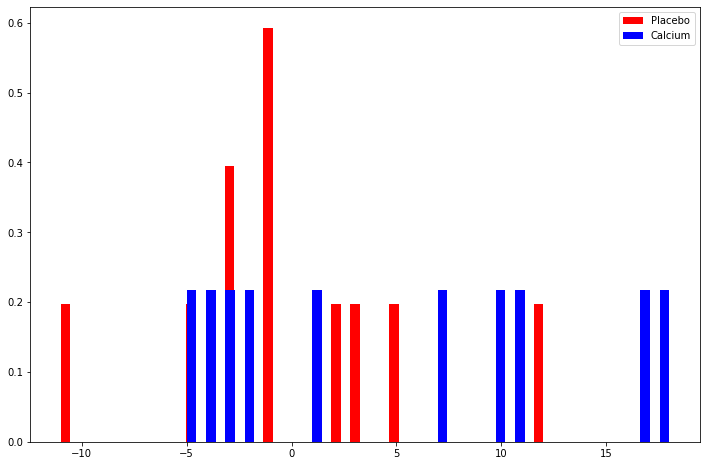
\includegraphics{Figure-16-01}
\end{figure}

First,  calculate D -- creating the empirical CDFs \(\hat{F}_{1}\)
and \(\hat{F}_{2}\), and then testing the value of \(D\) for each possible
\(x\) in the empirical distributions:

\begin{python}
f1 = data[data['Treatment'] == 'Placebo']['Decrease'].to_numpy()
f2 = data[data['Treatment'] == 'Calcium']['Decrease'].to_numpy()
def f1_hat(x):
    return sum(f1 <= x) / len(f1)
def f2_hat(x):
    return sum(f2 <= x) / len(f2)
xx = np.linspace(min(data['Decrease']) - 1, max(data['Decrease']) + 1, 100)
fig, (ax1, ax2) = plt.subplots(2, sharex=True, figsize=(12, 8))
ax1.plot(xx, [f1_hat(x) for x in xx], color='blue', label='F1 empirical distribution')
ax1.plot(xx, [f2_hat(x) for x in xx], color='red', label='F2 empirical distribution')
ax1.legend(loc='upper left')
ax2.plot(xx, [abs(f1_hat(x) - f2_hat(x)) for x in xx], color='purple', label='|F1 - F2|')
ax2.legend(loc='upper left')
plt.show()
\end{python}

\begin{python}
D = max([abs(f1_hat(x) - f2_hat(x)) for x in data['Decrease']])
n1 = len(f1)
n2 = len(f2)
test_statistic = np.sqrt(n1 * n2 / (n1 + n2)) * D
print('D: %.3f' % D)
print('Test statistic: %.3f' % test_statistic)
\end{python}
\begin{console}
D: 0.409
Test statistic: 0.936
\end{console}
Given that
\begin{align*}
H(t) &= 1 - 2 \sum_{j=1}^{\infty} (-1)^{j-1} e^{-2j^{2}t^{2}}
\end{align*}
 create an approximation for \(H^{-1}(1 - \alpha)\) -- so that we
may find the p-value for \(\alpha\) such that $
\sqrt{\frac{n_{1} n_{2}}{n_{1} + n_{2}}} D > H^{-1}(1 -
\alpha) $.

\begin{python}
def H(t, xtol=1e-8):
    assert t != 0, "t must be non-zero"
    t2 = t * t
    j_max = int(np.ceil(np.sqrt(- np.log(xtol / 2) / (2 * t2) )))
    jj = np.arange(1, j_max+1)
    return 1 + 2 * sum((-1)**(jj) * np.exp(-2 * (jj**2) * t2))
\end{python}

\begin{python}
# Plot some values for H(t)
tt = np.logspace(-3, 0.25, 100)
ht = [H(t) for t in tt]
plt.figure(figsize=(6, 4))
plt.plot(tt, ht)
plt.title('H(t)')
plt.show()
\end{python}

\begin{figure}[H]
\centering
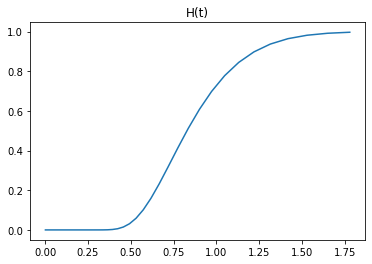
\includegraphics{Figure-16-03}
\end{figure}


\begin{python}
from scipy.optimize import minimize
def H_inv(q):
    def loss_function(x):
        return (H(x) - q)**2
    
    x0 = 1.0
    return minimize(loss_function, x0, method='nelder-mead').x
\end{python}

\begin{python}
# Plot some values for H_inv(q)
qq = np.linspace(1e-5, 1 - 1e-5, 200)
xx = [H_inv(q) for q in qq]
plt.figure(figsize=(6, 4))
plt.plot(qq, xx)
plt.title('H^{-1}(q)')
plt.show()
\end{python}

\begin{figure}[H]
\centering
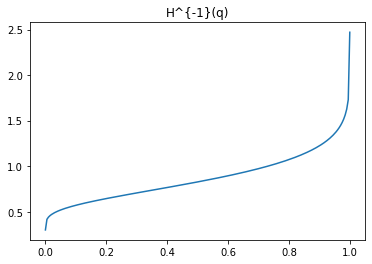
\includegraphics{Figure-16-04}
\end{figure}


\begin{python}
h_inv_test_statistic = H_inv(test_statistic)
print('Test statistic: \t\t%.3f' % test_statistic)
print('H^{-1}(test_statistic): \t%.3f' % h_inv_test_statistic)
\end{python}
\begin{console}
Test statistic:                 0.936
H^{-1}(test\_statistic):         1.313
\end{console}
Given that the inverse of the test statistic is greater than 1, we have
that the test from Theorem 16.16 rejects the null hypothesis for any
\(\alpha > 0\) -- so it claims the distributions are distinct at any
approximate \(\alpha\) level -- so, by Theorem 16.15, they are
associated.


% Chapter 17
\section*{17. Undirected Graphs and Conditional Independence}\label{undirected-graphs-and-conditional-independence}
\(k\) binary variables \(Y_{1}, \dots, Y_{k}\) correspond to a multinomial
with \(N = 2^{k}\) categories. Even for moderately large \(k\), \(2^{k}\)
will be huge. It can be shown in this case that the MLE is a poor
estimator, because the data are \textbf{sparse}.
Graphical models often require fewer parameters and may lead to
estimators with smaller risk. There are two main types of graphical
models: undirected and directed. Here we introduce undirected graphs.


\subsection*{17.1 Conditional Independence}\label{conditional-independence}
Let \(X\), \(Y\), \(Z\) be discrete random variables. We say that \(X\)
and \(Y\) are \textbf{conditionally independent given \(Z\)}, written
\(X \text{⫫} Y \;|\; Z\), if
\[
\PROB(X = x, Y = y | Z = z) = \PROB(X = x | Z = z) \PROB(Y = y | Z = z)
\]
for all \(x\), \(y\), \(z\). If \(X\), \(Y\), \(Z\) are continuous
random variables, we say that \(X\) and \(Y\) are conditionally
independent given \(Z\) if
\[
f_{X, Y | Z}(x, y | z) = f_{X | Z}(x | z) f_{Y | Z}(y | z)
\]
for all \(x\), \(y\), \(z\).
Intuitively, this means that once you know \(Z\), \(Y\) provides no
extra information about \(X\).

\textbf{Theorem 17.2}. The following implications hold:
\begin{align*}
X \ci Y \;|\; Z & \Longrightarrow Y \ci X \;|\; Z \\
X \ci Y \;|\; Z \; \text{and} \; U = h(X) & \Longrightarrow U \ci Y \;|\; Z \\
X \ci Y \;|\; Z \; \text{and} \; U = h(X) & \Longrightarrow X \ci Y \;|\; (Z, U)  \\
X \ci Y \;|\; Z \; \text{and} \; X \ci W \;|\; (Y, Z) & \Longrightarrow X \ci (W, Y) \;|\; Z \\
X \ci Y \;|\; Z \; \text{and} \; X \ci Z \;|\; Y \; & \Longrightarrow Y \ci (Y, Z)
\end{align*}
The last property requires the assumption that all events have positive
probability; the first four do not.


\subsection*{17.2 Undirected Graphs}\label{undirected-graphs}
An \textbf{undirected graph} \(\mathcal{G} = (V, E)\) has a finite set
\(V\) of \textbf{vertices} (or \textbf{nodes}) and a set \(E\) of
\textbf{edges} (or \textbf{arcs}) consisting of pairs of vertices. The
vertices correspond to random variables \(X, Y, Z, \dots\) and the edges
are written as unordered pairs. For example, \((X, Y) \in E\) means that
\(X\) and \(Y\) are joined by an edge.

\begin{python}
from graphviz import Graph
g = Graph()
g.edge('Y', 'X')
g.edge('Y', 'Z')
g
\end{python}

\begin{figure}[H]
\centering
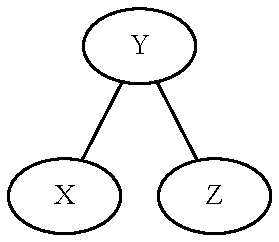
\includegraphics{Figure-17-01}
\end{figure}

\emph{A graph with vertices \(V = \{X, Y, Z\}\). The edge set is
\(E = \{(X, Y), (Y, Z)\}\).}
Two vertices are \textbf{adjacent}, written \(X \sim Y\), if there is an
edge between them. A sequence \(X_{0}, \dots, X_{n}\) is called a
\textbf{path} if \(X_{i-1} \sim X_{i}\) for each \(i\). A graph is
\textbf{complete} if there is an edge between every pair of vertices. A
subset \(U \subset V\) of vertices together with their edges is called a
\textbf{subgraph}.
If \(A\), \(B\) and \(C\) are three distinct subsets in \(V\), we say
that \textbf{\(C\) separates \(A\) and \(B\)} if every path from a
variable in \(A\) to a variable in \(B\) intersects a variable in \(C\).

\begin{python}
from graphviz import Graph
g = Graph()
g.edge('W', 'X')
g.edge('W', 'Y')
g.edge('X', 'Z')
g.edge('X', 'Y')
g
\end{python}

\begin{figure}[H]
\centering
\includegraphics{Figure-17-02}
\end{figure}

\emph{\(\{Y, W\}\) and \(\{Z\}\) are separated by \(\{X\}\). Also, \(W\)
and \(Z\) are separated by \(\{X, Y\}\).}

\subsection*{17.3 Probability and Graphs}\label{probability:graphs}
Let \(V\) be a set of random variables with distribution \(\PROB\).
Construct a graph with one vertex for each random variable in \(V\).
Suppose we omit the edge between a pair of variables if they are
independent given the rest of the variables:
\[
\text{no edge between } X \text{ and } Y \Leftrightarrow X \text{⫫} Y \;|\; \text{rest}
\]
where ``rest'' refers to all the other variables besides \(X\) and
\(Y\). This type of graph is called a \textbf{pairwise Markov graph}.
The graph encodes a set of pairwise conditional independence relations.
These relations imply other conditional independence relations.
Fortunately we can read these other conditional independence relations
from the graph as well, as is explained in the next Theorem.

\textbf{Theorem 17.3}. Let \(\mathcal{G} = (V, E)\) be a pairwise Markov
graph for a distribution \(\PROB\). Let \(A\), \(B\), and \(C\) be
distinct subsets of \(V\) such that \(C\) separates \(A\) and \(B\).
Then \(A \ci B \;|\; C\).
Remark: if \(A\) and \(B\) are not connected, we can regard them as
separated by the empty set. Then it follows from the Theorem that
\(A \ci B\).
The independence property in Theorem 17.3 is called the \textbf{global
Markov property}. We thus see that the pairwise and global Markov
properties are equivalent.
More precisely: given a graph \(\mathcal{G}\),
\begin{itemize}[tightlist]
\item
  Let \(M_\text{pair}(\mathcal{G})\) be the set of distributions that
  satisfy the pairwise Markov property; thus
  \(\PROB \in M_\text{pair}(\mathcal{G})\) if, under
  \(\PROB\), \(X \text{⫫} Y \;|\; \text{rest}\) if and only if
  there is no edge between \(X\) and \(Y\).
\item
  Let \(M_\text{global}(\mathcal{G})\) be the set of distributions that
  satisfy the global Markov property; thus
  \(\PROB \in M_\text{global}(\mathcal{G})\) if, under
  \(\PROB\), \(A \text{⫫} B \;|\; C\) if and only if \(C\)
  separates \(A\) and \(B\).
\end{itemize}

\textbf{Theorem 17.5}. Let \(\mathcal{G}\) be a graph. Then
\(M_\text{pair}(\mathcal{G}) = M_\text{global}(\mathcal{G})\).

\begin{python}
from graphviz import Graph
g = Graph()
g.edge('X', 'Y')
g.edge('Y', 'Z')
g.edge('Z', 'X')
g
\end{python}

\begin{figure}[H]
\centering
\includegraphics{Figure-17-03}
\end{figure}

\emph{No implied independence relations}

\begin{python}
from graphviz import Graph
g = Graph()
g.edge('X', 'Y')
g.edge('Y', 'Z')
g.edge('Z', 'W')
g.edge('W', 'X')
g
\end{python}

\begin{figure}[H]
\centering
\includegraphics{Figure-17-04}
\end{figure}

\emph{\(X \ci Z \;|\; \{Y, W\}\) and
\(Y \ci W \;|\; \{X, Z\}\)}

\begin{python}
from graphviz import Graph
g = Graph()
g.edge('X', 'Y')
g.edge('Y', 'Z')
g.edge('Z', 'W')
g
\end{python}

\begin{figure}[H]
\centering
\includegraphics{Figure-17-05}
\end{figure}

\emph{\(X \ci Z \;|\; Y\) and \(Y \ci W \;|\; Z\)}

\begin{python}
from graphviz import Graph
g = Graph()
g.edge('Y', 'Z')
g.node('X')
g
\end{python}

\begin{figure}[H]
\centering
\includegraphics{Figure-17-06}
\end{figure}

\emph{\(X \ci Y\), \(X \ci Z\) and
\(X \ci (Y, Z)\)}

\begin{python}
from graphviz import Graph
g = Graph()
g.edge('Y', 'W')
g.edge('W', 'Z')
g.edge('Z', 'Y')
g.edge('X', 'Y')
g
\end{python}

\begin{figure}[H]
\centering
\includegraphics{Figure-17-07}
\end{figure}

\emph{\(X \ci W | (Y, Z)\) and \(X \ci Z | Y\)}

\subsection*{17.4 Fitting Graphs to Data}\label{fitting-graphs-to-data}
Given a dataset, how do we find a graphical model that fits the data?
Some authors have devoted whole books to this subject. We will only
treat the discrete case and we will consider a method based on
\textbf{log-linear models} which are the subject of the next chapter.

\subsection*{17.6 Exercises}

\textbf{Exercise 17.6.1}. Consider random variables \((X_{1}, X_{2}, X_{3})\).
In each of the following cases, draw a graph that has the given
independence relations.
\textbf{(i)} \(X_{1} \ci X_{3} | X_{2}\)
\textbf{(ii)} \(X_{1} \ci X_{2} | X_{3}\) and
\(X_{1} \ci X_{3} | X_{2}\)
\textbf{(iii)} \(X_{1} \ci X_{2} | X_{3}\) and
\(X_{1} \ci X_{3} | X_{2}\) and \(X_{2} \ci X_{3} | X_{1}\)

\textbf{Solution}
\textbf{(i)} \(X_{1} \ci X_{3} | X_{2}\)

\begin{python}
from graphviz import Graph
g = Graph()
g.edge('X1', 'X2')
g.edge('X2', 'X3')
g
\end{python}

\begin{figure}[H]
\centering
\includegraphics{Figure-17-08}
\end{figure}

\textbf{(ii)} \(X_{1} \ci X_{2} | X_{3}\) and
\(X_{1} \ci X_{3} | X_{2}\)

\begin{python}
from graphviz import Graph
g = Graph()
g.node('X1')
g.edge('X2', 'X3')
g
\end{python}

\begin{figure}[H]
\centering
\includegraphics{Figure-17-09}
\end{figure}

\textbf{(iii)} \(X_{1} \ci X_{2} | X_{3}\) and
\(X_{1} \ci X_{3} | X_{2}\) and \(X_{2} \ci X_{3} | X_{1}\)

\begin{python}
from graphviz import Graph
g = Graph()
g.node('X1')
g.node('X2')
g.node('X3')
g
\end{python}

\begin{figure}[H]
\centering
\includegraphics{Figure-17-10}
\end{figure}


\textbf{Exercise 17.6.2}. Consider random variables
\((X_{1}, X_{2}, X_{3}, X_{4})\). In each of the following cases, draw a graph
that has the given independence relations.
\textbf{(a)} $X\_{1} \ci X\_{3} | X\_{2}, X\_{4} $ and $X\_{1}
\ci X\_{4} | X\_{2}, X\_{3} $ and $X\_{2} \ci X\_{4}
| X\_{1}, X\_{3} $
\textbf{(b)} $X\_{1} \ci X\_{2} | X\_{3}, X\_{4} $ and $X\_{1}
\ci X\_{3} | X\_{2}, X\_{4} $ and $X\_{2} \ci X\_{3}
| X\_{1}, X\_{4} $
\textbf{(c)} $X\_{1} \ci X\_{3} | X\_{2}, X\_{4} $ and $X\_{2}
\ci X\_{4} | X\_{1}, X\_{3} $

\textbf{Solution}
\textbf{(a)} $X\_{1} \ci X\_{3} | X\_{2}, X\_{4} $ and $X\_{1}
\ci X\_{4} | X\_{2}, X\_{3} $ and $X\_{2} \ci X\_{4}
| X\_{1}, X\_{3} $

\begin{python}
from graphviz import Graph
g = Graph()
g.edge('X1', 'X2')
g.edge('X2', 'X3')
g.edge('X3', 'X4')
g
\end{python}

\begin{figure}[H]
\centering
\includegraphics{Figure-17-11}
\end{figure}

\textbf{(b)} $X\_{1} \ci X\_{2} | X\_{3}, X\_{4} $ and $X\_{1}
\ci X\_{3} | X\_{2}, X\_{4} $ and $X\_{2} \ci X\_{3}
| X\_{1}, X\_{4} $

\begin{python}
from graphviz import Graph
g = Graph()
g.edge('X1', 'X4')
g.edge('X2', 'X4')
g.edge('X3', 'X4')
g
\end{python}

\begin{figure}[H]
\centering
\includegraphics{Figure-17-12}
\end{figure}

\textbf{(c)} $X\_{1} \ci X\_{3} | X\_{2}, X\_{4} $ and $X\_{2}
\ci X\_{4} | X\_{1}, X\_{3} $

\begin{python}
from graphviz import Graph
g = Graph()
g.edge('X1', 'X2')
g.edge('X2', 'X3')
g.edge('X3', 'X4')
g.edge('X1', 'X4')
g
\end{python}

\begin{figure}[H]
\centering
\includegraphics{Figure-17-13}
\end{figure}


\textbf{Exercise 17.6.3}. A conditional independence between a pair of
variables is \textbf{minimal} if it is not possible to use the
Separation Theorem to eliminate any variable from the conditioning set,
i.e.~from the right side of the bar (Whittaker 1990). Write down the
minimal conditioning independences from the given figures.
\textbf{(a)}

\begin{python}
from graphviz import Graph
g = Graph()
g.edge('X1', 'X2')
g.edge('X2', 'X3')
g.edge('X2', 'X4')
g
\end{python}

\begin{figure}[H]
\centering
\includegraphics{Figure-17-14}
\end{figure}

\textbf{(b)}

\begin{python}
from graphviz import Graph
g = Graph()
g.edge('X1', 'X2')
g.edge('X2', 'X3')
g.edge('X3', 'X4')
g
\end{python}

\begin{figure}[H]
\centering
\includegraphics{Figure-17-15}
\end{figure}

\textbf{(c)}

\begin{python}
from graphviz import Graph
g = Graph()
g.edge('X1', 'X2')
g.edge('X2', 'X3')
g.edge('X3', 'X4')
g.edge('X4', 'X1')
g
\end{python}

\begin{figure}[H]
\centering
\includegraphics{Figure-17-16}
\end{figure}

\textbf{(d)}

\begin{python}
from graphviz import Graph
g = Graph()
g.edge('X1', 'X2')
g.edge('X2', 'X3')
g.edge('X3', 'X1')
g.edge('X2', 'X4')
g.edge('X4', 'X5')
g.edge('X5', 'X2')
g.edge('X3', 'X5')
g.edge('X5', 'X6')
g.edge('X6', 'X3')
g
\end{python}

\begin{figure}[H]
\centering
\includegraphics{Figure-17-17}
\end{figure}


\textbf{Solution}
\textbf{(a)}
\begin{itemize}[tightlist]
\item
  $X\_{1} \ci X\_{3} | X\_{2} $
\item
  $X\_{1} \ci X\_{4} | X\_{2} $
\item
  $X\_{3} \ci X\_{4} | X\_{2} $
\end{itemize}
\textbf{(b)}
\begin{itemize}[tightlist]
\item
  $X\_{1} \ci X\_{3} | X\_{2} $
\item
  $X\_{2} \ci X\_{4} | X\_{2} $
\item
  $X\_{1} \ci X\_{4} | X\_{2} $ (or $X\_{1} \ci X\_{4}
  | X\_{3} $)
\end{itemize}
\textbf{(c)}
\begin{itemize}[tightlist]
\item
  $X\_{1} \ci X\_{3} | X\_{2}, X\_{4} $
\item
  $X\_{2} \ci X\_{4} | X\_{1}, X\_{3} $
\end{itemize}
\textbf{(d)}
\begin{itemize}[tightlist]
\item
  $X\_{1} \ci X\_{4} | X\_{2}, X\_{3} $ ( or $X\_{1} \ci 
  X\_{4} | X\_{2}, X\_{5} $ )
\item
  $X\_{1} \ci X\_{5} | X\_{2}, X\_{3} $
\item
  $X\_{1} \ci X\_{6} | X\_{2}, X\_{3} $ ( or $X\_{1} \ci 
  X\_{6} | X\_{2}, X\_{5} $ )
\item
  $X\_{2} \ci X\_{6} | X\_{3}, X\_{5} $
\item
  $X\_{3} \ci X\_{4} | X\_{2}, X\_{5} $
\item
  $X\_{4} \ci X\_{6} | X\_{2}, X\_{5} $ ( or $X\_{4} \ci 
  X\_{6} | X\_{3}, X\_{5} $ )
\end{itemize}

\textbf{Exercise 17.6.4}. Here are the breast cancer data on diagnosic
center (\(X_{1}\)), nuclear grade (\(X_{2}\)) and survival (\(X_{3}\)):
\[
\begin{array}{cccccc}
    & X_{2} & \text{malignant} & \text{malignant} & \text{benign} & \text{benign}   \\
    & X_{3} & \text{died}      & \text{survived}  & \text{died}   & \text{survived} \\
\hline
X_{1} & \text{Boston}    & 35 & 59 & 47 & 112 \\
    & \text{Glamorgan} & 42 & 77 & 26 & 76 \\
\hline
\end{array}
\]
\textbf{(a)} Treat this as a multinomial and find the maximum likelihood
estimator.
\textbf{(b)} If someone has a tumour classified as benign at the
Glamorgan clinic, what is the estimated probability that they will die?
Find the standard error for this estimate.
\textbf{(c)} Test the following hypothesis:
\begin{align*}
X_{1} \ci X_{2} |  X_{3} \quad &\text{versus} \quad \text{not} (X_{1} \ci X_{2} |  X_{3} ) \\
X_{1} \ci X_{3} |  X_{2} \quad &\text{versus} \quad \text{not} (X_{1} \ci X_{3} |  X_{2} ) \\
X_{2} \ci X_{3} |  X_{1} \quad &\text{versus} \quad \text{not} (X_{2} \ci X_{3} |  X_{1} ) \\
\end{align*}
Based on the results of your tests, draw and interpret the resulting
graph.

\textbf{Solution}.
\textbf{(a)}

\begin{python}
import numpy as np
X = np.array([[[35, 59], [47, 112]], [[42, 77], [26, 76]]])
\end{python}

\begin{python}
p_hat = X / X.sum()
p_hat
\end{python}
\begin{console}
array([[[0.07383966, 0.12447257],
        [0.09915612, 0.23628692]],
       [[0.08860759, 0.16244726],
        [0.05485232, 0.16033755]]])
\end{console}
\textbf{(b)} The question asks for
\(\PROB( X_{3} = \text{died} | X_{1} = \text{Glamorgan}, X_{2} = \text{benign})\).
The MLE estimate is:
\[
\hat{p} = \frac{26}{26 + 76} \approx 0.2594
\]
The distribution is a binomial distribution on only \(X_{3}\), conditioned
on the other variables.
The variance is
\[
\VAR(\hat{p}) = \frac{1}{n}\hat{p} (1 - \hat{p}) = \frac{1}{26 + 76} \frac{26}{26 + 76} \frac{76}{26 + 76}  \approx 0.001862
\]
so the standard deviation of this estimate is approximately \(0.0431\).
\textbf{(c)}
We will test conditional independence \(A \ci B \;|\; C\) over
discrete variables \(A\), \(B\) and \(C\) by testing independence
between \(A\) and \(B\) for each value of \(C = c\) and then selecting
the largest / worst p-value.

\begin{python}
from scipy.stats import chi2_contingency
def get_p_value(table):
    # Implement Pearson's chi squared independence test
    chi2, p, dof, expected = chi2_contingency(table)
    return p
\end{python}

\begin{python}
p_12 = max([get_p_value(X[:, :, k]) for k in range(X.shape[2])])
p_13 = max([get_p_value(X[:, k, :]) for k in range(X.shape[1])])
p_23 = max([get_p_value(X[k, :, :]) for k in range(X.shape[1])])
print("X_1 ⫫ X_2 | X_3:  %.3f" % p_12)
print("X_1 ⫫ X_3 | X_2:  %.3f" % p_13)
print("X_2 ⫫ X_3 | X_1:  %.3f" % p_23)
\end{python}
\begin{console}
X_1 ⫫ X_2 | X_3:  0.030
X_1 ⫫ X_3 | X_2:  0.882
X_2 ⫫ X_3 | X_1:  0.262
\end{console}
At a confidence level of 5\%, we can certify the first hypothesis, but
not the other two.
The resulting graph would be:

\begin{python}
from graphviz import Graph
g = Graph()
g.edge('X1 (diagnostic center)', 'X3 (survival)')
g.edge('X3 (survival)', 'X2 (nuclear grade)')
g
\end{python}

\begin{figure}[H]
\centering
\includegraphics{Figure-17-18}
\end{figure}
These results can be interpreted to mean that the nuclear grade is
independent of the diagnostic center given the survival -- that is, no
diagnostic center is more optimistic or pessimistic in its
classification of tumors given their severity.


% Chapter 18
\section*{18. Loglinear Models}\label{loglinear-models}

\subsection*{18.1 The Loglinear Model}\label{the-loglinear-model}

Let \(X = (X_{1}, \dots, X_m)\) be a random vector with probability

\[ f(x) = \mathbb{P}(X = x) = \mathbb{P}(X_{1} = x_{1}, \dots, X_m = x_m) \]

Let \(r_{j}\) be the number of values that \(X_{j}\) takes; without loss of
generality, assume \(X_{j} \in \{ 0, 1, \dots, r_{j} - 1 \}\). Suppose we
have \(n\) such vectors.

We can think of the data as a sample from a Multinomial with
\(N = r_{1} \times r_{2} \times \dots \times r_m\) categories. The data can
be represented as counts in a \(r_{1} \times r_{2} \times \dots \times r_m\)
table. Let \(p = \{ p_{1}, \dots, p_N \}\) denote the multinomial
parameter.

Let \(S = \{ 1, \dots, m \}\). Given a vector \(x = (x_{1}, \dots, x_m)\)
and a subset \(A \subset S\), let \(x_A = (x_{j} : j \in A)\). For
example, if \(A = \{1, 3\}\) then \(x_A = (x_{1}, x_{3})\).

\textbf{Theorem 18.1}. The joint probability function \(f(x)\) of a
single random vector \(X = (X_{1}, \dots, X_m)\) can be written as

\[ \log f(x) = \sum_{A \subset S} \psi_A(x) \]

where the sum is over all subsets \(A\) of \(S = \{1, \dots, m \}\) and
the \(\psi\)s satisfy the following conditions:

\begin{enumerate}[tightlist,label={\arabic*.}]
\item
  \(\psi_\varnothing(x)\) is a constant;
\item
  For every \(A \subset S\), \(\psi_A(x)\) is only a function of \(x_A\)
  and not the rest of the \(x_{j}\)s.
\item
  If \(i \in A\) and \(x_{i} = 0\), then \(\psi_A(x) = 0\).
\end{enumerate}

The formula in this Theorem is known as the \textbf{log-linear
expansion} of \(f\). Note that this is the probability function for a
single draw. Each \(\psi_A(x)\) will depend on some unknown parameters
\(\beta_A\). Let \(\beta = (\beta_A : A \subset S)\) be the set of all
these parameters. We will write \(f(x) = f(x; \beta)\) when we want to
estimate the dependence on the unknown parameters \(\beta\).

In terms of the multinomial, the parameter space is

\[ \mathcal{P} = \left\{ p = (p_{1}, \dots, p_N) : p_{j} \geq 0, \sum_{j=1}^N p_{j} = 1 \right\} \]

This is an \(N - 1\) dimensional space. In the log-linear
representation, the parameter space is

\[ \Theta = \Bigg\{ \beta = (\beta_{1}, \dots, \beta_N) : \beta = \beta(p), p \in \mathcal{P} \Bigg\} \]

where \(\beta(p)\) is the set of \(\beta\) values associated with \(p\).
The set \(\Theta\) is a \(N - 1\) dimensional surface in
\(\mathbb{R}^N\). We can always go back and forth between the two
parametrizations by writing \(\beta = \beta(p)\) and \(p = p(\beta)\).

\textbf{Theorem 18.14}. Let \((X_a, X_b, X_c)\) be a partition of
vectors \((X_{1}, \dots, X_m)\). Then \(X_b \text{ ⫫ } X_c \; | \; X_a\)
if and only if all the \(\psi\)-terms in the log-linear expansion that
have at least one coordinate in \(b\) and one coordinate in \(c\) are 0.

To prove this Theorem, we will use the following Lemma whose proof
follows from the definition of conditional independence.

\textbf{Lemma 18.5}. A partition \((X_a, X_b, X_c)\) satisfies
\(X_b \text{ ⫫ } X_c \; | \; X_a\) if and only if
\(f(x_a, x_b, x_c) = g(x_a, x_b) h(x_a, x_c)\) for some functions \(g\)
and \(h\).

\textbf{Proof of Theorem 18.14}. Suppose that \(\psi_t\) is 0 whenever
\(t\) has coordinates in \(b\) and \(c\). Hence, \(\psi_t\) is 0 if
\(t\) is not a subset of \(a \cup b\) or \(t\) is not a subset of
\(a \cup c\). Therefore,

\[ \log f(x) = \sum_{t \subset a \cup b} \psi_t(x) + \sum_{t \subset a \cup c} \psi_t(x) - \sum_{t \subset a} \psi_t(x) \]

Exponentiating, we see that the joint density is of the form
\(g(x_a, x_b) h(x_a, x_c)\). By Lemma 18.5,
\(X_b \text{ ⫫ } X_c \; | \; X_a\). The converse follows by reversing
the argument.

\subsection*{18.2 Graphical Log-Linear Models}\label{graphical-log-linear-models}

Let \(\log f(x) = \sum_{A \subset S} \psi_A(x)\) be a log-linear model.
Then \(f\) is \textbf{graphical} if all \(\psi\)-terms are non-zero
except for any pair of coordinates not in the edge set for some graph
\(\mathcal{G}\). In other words, \(\psi_A(x) = 0\) if and only if
\(\{i, j\} \subset A\) and \((i, j)\) is not an edge.

Here is a way to think about this definition: if you can add a term to
the model and the graph does not change, then the model is not
graphical.

\subsection*{18.3 Hierarchical Log-Linear Models}\label{hierarchical-log-linear-models}

There is a set of log-linear models that is larger than the set of
graphical models and that are used quite a bit. These are hierarchical
log-linear models.

A log-linear model is \textbf{hierarchical} if \(\psi_a = 0\) and
\(a \subset t\) implies that \(\psi_t = 0\).

\textbf{Lemma 18.9}. A graphical model is hierarchical but the reverse
need not be true.

\subsection*{18.4 Model Generators}\label{model-generators}

Hierarchical models can be written succintly using \textbf{generators}.
This is most easily explained by example. Suppose that
\(X = (X_{1}, X_{2}, X_{3})\). Then, \(M = 1.2 + 1.3\) stands for:

\[ \log f = \psi_\varnothing + \psi_{1} + \psi_{2} + \psi_{3} + \psi_{12} + \psi_{13}\]

The formula \(M = 1.2 + 1.3\) says: ``include \(\psi_{12}\) and
\(\psi_{13}\)''. We have to also include the lower terms or it will not be
hierarchical. The generator \(M = 1.2.3\) is the \textbf{saturated}
model

\[ \log f = \psi_\varnothing + \psi_{1} + \psi_{2} + \psi_{3} + \psi_{12} + \psi_{13} + \psi_{23} + \psi_{123}\]

The saturated models corresponds to fitting and unconstrained
multinomial. Consider \(M = 1 + 2 + 3\) which means

\[ \log f = \psi_\varnothing + \psi_{1} + \psi_{2} + \psi_{3} \]

This is the mutual independence model. Finally, consider \(M = 1.2\)
which has log-linear expansion

\[ \log f = \psi_\varnothing + \psi_{1} + \psi_{2} + \psi_{12} \]

This models makes \(X_{3} | X_{2} = x_{2}, X_{1} = x_{1}\) a uniform distribution.

\subsection*{18.5 Lattices}\label{lattices}

Hierarchical models can be organized into something called a
\textbf{lattice}. This is the set of all hierarchical models partially
ordered by inclusion. The set of all hierarchical models for two
variables can be illustrated as in the figure below.

\begin{python}
from graphviz import Digraph

d = Digraph()

d.edge('1.2', '1 + 2')
d.edge('1 + 2', '1')
d.edge('1 + 2', '2')
d.edge('1', '0')
d.edge('2', '0')

d
\end{python}
 
\begin{figure}[H]
\centering
\includegraphics{Figure-18-01}
\end{figure}

\(M = 1.2\) is the saturated model, \(M = 1 + 2\) is the independence
model, \(M = 1\) is the independence model plus \(X_{2} | X_{1}\) is
uniform, \(M = 2\) is the independence model plus \(X_{1} | X_{2}\) is
uniform, \(M = 0\) is the uniform distribution.

The lattice of trivariate models is shown in the figure below:

\begin{python}
from graphviz import Digraph

d = Digraph()

d.edge('1.2.3', '1.2 + 1.3 + 2.3')

d.edge('1.2 + 1.3 + 2.3', '1.2 + 1.3')
d.edge('1.2 + 1.3 + 2.3', '1.2 + 2.3')
d.edge('1.2 + 1.3 + 2.3', '1.3 + 2.3')

d.edge('1.2 + 1.3', '1.2 + 3')
d.edge('1.2 + 2.3', '1.2 + 3')

d.edge('1.2 + 1.3', '1.3 + 2')
d.edge('1.3 + 2.3', '1.3 + 2')

d.edge('1.2 + 2.3', '2.3 + 1')
d.edge('1.3 + 2.3', '2.3 + 1')

d.edge('1.2 + 3', '1 + 2 + 3')
d.edge('1.3 + 2', '1 + 2 + 3')
d.edge('2.3 + 1', '1 + 2 + 3')

d.edge('1.2 + 3', '1.2')
d.edge('1.3 + 2', '1.3')
d.edge('2.3 + 1', '2.3')

d.edge('1.2', '1 + 2')
d.edge('1.3', '1 + 3')
d.edge('2.3', '2 + 3')

d.edge('1 + 2 + 3', '1 + 2')
d.edge('1 + 2 + 3', '1 + 3')
d.edge('1 + 2 + 3', '2 + 3')

d.edge('1 + 2', '1')
d.edge('1 + 2', '2')
d.edge('1 + 3', '1')
d.edge('1 + 3', '3')
d.edge('2 + 3', '2')
d.edge('2 + 3', '3')

d.edge('1', '0')
d.edge('2', '0')
d.edge('3', '0')

d
\end{python}
 
\begin{figure}[H]
\centering
\includegraphics{Figure-18-02}
\end{figure}

\subsection*{18.6 Fitting Log-Linear Models to Data}\label{fitting-log-linear-models-to-data}

Let \(\beta\) denote all the parameters in a log-linear model \(M\). The log-likelihood for \(\beta\) is:

\[ \ell(\beta) = \sum_{j} x_{j} \log p_{j}(\beta) \]

where the sum is over the cells and \(p(\beta)\) denotes the cell probabilities corresponding to \(\beta\). The MLE \(\hat{\beta}\) generally has to be found numerically. The model with all possible \(\psi\)-terms is called the \textbf{saturated models}. We can also fit any \textbf{sub-model} which corresponds to setting some subset of \(\psi\) terms to 0.

For any submodel \(M\), define the \textbf{deviance} \(\text{dev}(M)\) by
\[ \text{dev}(M) = 2 (\hat{\ell}_\text{sat} - \hat{\ell}_M) \]

where \(\ell_\text{sat}\) is the log-likelihood of the saturated model evaluated at the MLE and \(\hat{\ell}_M\) is the log-likelihood of the model \(M\) evaluated at its MLE.

\textbf{Theorem 18.14}. The deviance is the likelihood test statistic for

\[
H_{0} : \text{the model is } M
\quad \text{versus} \quad
H_{1} : \text{the model is not } M
\]

Under \(H_{0}\), \(\text{dev}(M) \leadsto \chi^{2}_\nu\) with \(\nu\) degrees of freedom equal to the difference in the number of parameters between the saturated model and \(M\).

One way to find a good model is to use the deviance to test every sub-model. Every model that is not rejected by this test is then considered a plausible model. However, this is not a good strategy for two reasons. First, we will end up doing many tests, which means there is ample opportunity for making Type I and Type II errors. Second, we will end up using models where we failed to reject \(H_{0}\). But we might fail to reject \(H_{0}\) due to low power. The result is that we end up with a bad model just due to low power.

There are many model searching strategies. A common approach is to use some form of \emph{penalized likelihood}. One version of penalized is the AIC that we used in regression. For any model \(M\), define
\[ 
\text{AIC}(M) = -2 \left( \hat{\ell}(M) - |M|\right) 
\]
where \(|M|\) is the number of parameters.

Consider a set of models \(\{ M_{1}, M_{2}, \dots \}\). Let \(\hat{f}_{j}(x)\) denote the estimated probability function obtained by using the maximum likelihood estimator of model \(M_{j}\). Thus, \(\hat{f}_{j}(x) = \hat{f}(x; \hat{\beta}_{j})\) where \(\hat{\beta}_{j}\) is the MLE of the set of parameters \(\beta_{j}\) for model \(M_{j}\). We will use the loss function \(D(f, \hat{f})\) where

\[ D(f, g) = \sum_x f(x) \log \frac{f(x)}{g(x)} \]

is the Kullback-Leibler divergence between two probability density functions. The corresponding risk function is \(R(f, \hat{f}) = \mathbb{E}(D(f, \hat{f}))\).

Notice that \(D(f, \hat{f}) = c - A(f, \hat{f})\) where \(c = \sum_x f(x) \log f(x)\) does not depend on \(\hat{f}\) and

\[ A(f, \hat{f}) = \sum_x f(x) \log \hat{f}(x) \]

Thus minimizing the risk is equivalent to minimizing \(a(f, \hat{f}) = \mathbb{E}(A(f, \hat{f}))\).

It is tempting to estimate \(a(f, \hat{f})\) by \(\sum_x \log \hat{f}(x)\) but, just as the training error in regression is highly biased estimate of prediction risk, it is also the case that \(\sum_x \log \hat{f}(x)\) is a highly biased estimate of \(a(f, \hat{f})\). In fact, the bias is approximately equal to \(|M_{j}|\). Thus:

\textbf{Theorem 18.15}. \(\text{AIC}(M_{j})\) is an approximately unbiased estimate of \(a(f, \hat{f})\).

After finding a ``best model'' this way we can draw the corresponding graph. We can also check the overall fit of the selected model using the deviance as described above.

\subsection*{18.8 Exercises}

\textbf{Exercise 18.8.1}. Solve for the \(p_{ij}\)s in terms of the \(\beta\)s in Example 18.3:

\emph{Example}: Let \(X = (X_{1}, X_{2})\) where \(X_{1} \in \{0, 1\}\) and \(X_{2} \in \{ 0, 1, 2 \}\). The joint distribution of \(n\) such random vectors is a multinomial with 6 categories. The multinomial parameters can be written as a 2-by-3 table as follows:

\[
\begin{array}{ccccc}
\hline
\text{multinomial} & x_{2} & 0 & 1 & 2 \\
\hline
x_{1} & 0 & p_{00} & p_{01} & p_{02} \\
    & 1 & p_{10} & p_{11} & p_{12} \\
\hline
\end{array}
\]

The \(n\) data vectors can be summarized as follows:

\[
\begin{array}{ccccc}
\hline
\text{multinomial} & x_{2} & 0 & 1 & 2 \\
\hline
x_{1} & 0 & C_{00} & C_{01} & C_{02} \\
    & 1 & C_{10} & C_{11} & C_{12} \\
\hline
\end{array}
\]

For \(x = (x_{1}, x_{2})\), the log-linear expansion takes the form

\[
\log f(x) = \psi_\varnothing(x) + \psi_{1}(x) + \psi_{2}(x) + \psi_{12}(x)
\]

where

\begin{align*}
& \psi_\varnothing(x) = \log p_{00} \\
& \psi_{1}(x) = x_{1} \log \left( \frac{p_{10}}{p_{00}} \right) \\
& \psi_{2}(x) = I(x_{2} = 1) \log \left( \frac{p_{01}}{p_{00}} \right) 
            + I(x_{2} = 2) \log \left( \frac{p_{02}}{p_{00}} \right) \\
& \psi_{12}(x) = I(x_{1} = 1, x_{2} = 1) \log \left( \frac{p_{11}p_{00}}{p_{01}p_{10}} \right)
               + I(x_{1} = 1, x_{2} = 2) \log \left( \frac{p_{12}p_{00}}{p_{02}p_{10}} \right)
\end{align*}

The six parameters of this model are:

\[
\begin{array}{ccc}
\beta_{1} = \log p_{00} &
\beta_{2} = \log \left( \frac{p_{10}}{p_{00}} \right) &
\beta_{3} = \log \left( \frac{p_{01}}{p_{00}} \right) \\
\beta_{4} = \log \left( \frac{p_{02}}{p_{00}} \right) &
\beta_{5} = \log \left( \frac{p_{11}p_{00}}{p_{01}p_{10}} \right) &
\beta_{6} = \log \left( \frac{p_{12}p_{00}}{p_{02}p_{10}} \right)
\end{array}
\]

\textbf{Solution}.

Exponentiate the six definitions for \(\beta_{k}\) above and get:

\[
\begin{array}{ccc}
p_{00} = \exp \beta_{1} &
\frac{p_{10}}{p_{00}} = \exp \beta_{2} &
\frac{p_{01}}{p_{00}} = \exp \beta_{3} \\
\frac{p_{02}}{p_{00}} = \exp \beta_{4} &
\frac{p_{11}p_{00}}{p_{01}p_{10}} = \exp \beta_{5} &
\frac{p_{12}p_{00}}{p_{02}p_{10}} = \exp \beta_{6}
\end{array}
\]

and then, isolating the \(p_{ij}\)s,

\[
\begin{array}{ccc}
p_{00} = \exp \beta_{1} &
p_{10} = \exp \left( \beta_{1} + \beta_{2} \right) &
p_{01} = \exp \left( \beta_{1} + \beta_{3} \right) \\
p_{02} = \exp \left( \beta_{1} + \beta_{4} \right) &
p_{11} = \exp \left( \beta_{1} + \beta_{2} + \beta_{3} + \beta_{5} \right) &
p_{12} = \exp \left( \beta_{1} + \beta_{2} + \beta_{4} + \beta_{6} \right)
\end{array}
\]

\textbf{Exercise 18.8.2}. Repeat example 18.17 using 7 covariates and
\(n = 1000\). To avoid numerical problems, replace any zero count with a
one.

\emph{Example}: Here is a synthetic example. We generate \(n = 100\)
random vectors \(X = (X_{1}, \dots, X_{5})\) of length 5. We generated the
data as follows:

\[ X_{1} \sim \text{Bernoulli}(1/2)\]

and

\[ X_{j} | X_{1}, \dots, X_{j-1} = \begin{cases}
1/4 & \text{if } X_{j-1} = 0 \\
3/4 & \text{if } X_{j-1} = 1
\end{cases}\]

It follows that

\begin{align*}
f(x_{1}, \dots, x_{5}) &= 
\left( \frac{1}{2} \right) \left( \frac{3}{4} \right)^{x_{1}} \left( \frac{1}{4} \right)^{1 - x_{1}} \left( \frac{3}{4} \right)^{x_{2}} \left( \frac{1}{4} \right)^{1 - x_{2}} \left( \frac{3}{4} \right)^{x_{3}} \left( \frac{1}{4} \right)^{1 - x_{3}} \left( \frac{3}{4} \right)^{x_{4}} \left( \frac{1}{4} \right)^{1 - x_{4}} \\
&= \left( \frac{1}{2} \right) \left( \frac{3}{4} \right)^{x_{1} + x_{2} + x_{3} + x_{4}} \left( \frac{1}{4} \right)^{4 - (x_{1} + x_{2} + x_{3} + x_{4})} 
\end{align*}

We estimated \(f\) using three methods: (i) maximum likelihood treating
this as a multinomial with 32 categories (ii) maximum likelihood from
the best loglinear model using AIC and forward selection and (iii)
maximum likelihood from the best loglinear model using BIC and forward
selection. We estimated the risk by simulating the sample 100 times. The
average risks were:

\begin{tabular}{@{}ll@{}}
\toprule
Method & Risk \\
\midrule
MLE & 0.63 \\
AIC & 0.54 \\
BIC & 0.53 \\
\bottomrule
\end{tabular}

In this example, there is little difference between AIC and BIC. Both
are better than maximum likelihood.

\textbf{Solution}.

Generate \(n = 1000\) random vectors \(X = (X_{1}, \dots, X_{k})\) of
length \(k = 7\) as follows:

\[ X_{1} \sim \text{Bernoulli}(1/2) 
\quad \text{and} \quad
X_{j} | X_{1}, \dots, X_{j-1} = \begin{cases}
1/4 & \text{if } X_{j-1} = 0 \\
3/4 & \text{if } X_{j-1} = 1
\end{cases}
\]

It follows that

\[ f(x) = \frac{1}{2} \left( \frac{3}{4} \right)^{\sum_{i=1}^{k - 1} x_{i}} \left( \frac{1}{4} \right)^{(k - 1) - \left(\sum_{i=1}^{k - 1} x_{i} \right)} \]

We will use the KL divergence as our loss function:

\[ D(f, g) = \sum_{x \in \Omega} f(x) \log \frac{f(x)}{g(x)} \]

and estimate the risk function
\(R(f, \hat{f}) = \mathbb{E}[D(f, \hat{f})]\) by bootstraping the
estimation process and calculating the average of the loss functions in
each bootstrap step.

\paragraph{MLE estimate}\label{mle-estimate}

The MLE estimate for the full multinomial model is relatively simple:
consider the adjusted counts \(\tilde{C}_{\xi}\) to be the number of
times an observation \(\xi\) appears, or 1 if that number of
observations is 0. There are \(2^{k} = 128\) possible observations, so we
get \(2^{k}\) adjusted counts \(\tilde{C}_{1}, \dots, \tilde{C}_{2^{k}}\). The
MLE estimate is then computed as
\(\hat{p} = (\hat{p}_{1}, \dots, \hat{p}_{2^{k}})\), with
\(\hat{p}_{i} = \frac{\tilde{C}_{i}}{\sum_\xi \tilde{C}_\xi}\).

The function density estimate corresponding to the MLE estimate is a
simple lookup table \(\hat{f}(\xi) = \hat{p}_\xi\), as we already have a
probability estimate associated with every single possible event. The
function density estimate can then be used to compute the loss function
\(D(f, \hat{f})\), which is the KL divergence computed over the
universe. Repeating this process gives us the risk estimate.

\begin{python}
import numpy as np
from itertools import chain, combinations
from tqdm import tqdm_{n}otebook

def powerset(iterable):
    "powerset([1,2,3]) --> () (1,) (2,) (3,) (1,2) (1,3) (2,3) (1,2,3)"
    s = list(iterable)
    return chain.from_{i}terable(combinations(s, r) for r in range(len(s)+1))


def generate_samples(n, k):
    """
    Generates n samples of size k according to the synthetic distribution
    
    Args:
       n:  number of samples
       k:  sample size
       
    Returns:
       X:  2D array of shape (n, k), representing n samples of size k
    """
    
    # Generate a random unifom value between 0 and 1 for each variable in each sample
    random_seeds = np.random.uniform(low=0, high=1, size=(k, n))
    
    # Create a variable to store the generated samples
    output = np.empty_like(random_seeds).astype(int)
    
    # Generate x_{1}s as Bernoulli(1/2)
    output[0] = random_seeds[0] > 0.5
    for j in range(1, k):
        # Generate x_{j}s recursively
        output[j] = random_seeds[j] > (output[j - 1] == 0) * (1/4) + (output[j - 1] == 1) * (3/4)
        
    return output.T


def generate_universe(k):
    """
    Generates 2**k samples of size k iterating through the valid universe
    
    Args:
       k: sample size
       
    Returns:
       X_universe:  2D array of shape (2**k, k), representing the universe of all samples of size k
    """
    X_universe = np.zeros(shape=(2**k, k), dtype=int)
    for i, line in enumerate(powerset(range(k))):
        X_universe[i, line] = 1
        
    return X_universe


def row_to_binary(x):
    """
    Translates a single row into a binary low-endian representation
    
    Args:
       x:  1D array of 0s and 1s
       
    Returns:
       sum(x[i] * (2**i) for index i)
    """
    
    # Translate a row of 0s and 1s into a binary representation (low-endian)
    return sum([x[i] * (2**i) for i in range(len(x))])


def samples_to_count(X):
    """
    Counts the number of occurrences of each sample in the dataset
    
    Args:
       X:   2D array  n samples of size k
       
    Returns:
       count:  1D array of size 2**k, where count[i] is the number of
               occurrences of i as a row in binary (low-endian) in X,
               or 1 if the count would be 0.
    """
    
    binary_samples = np.apply_along_axis(row_to_binary, 1, X)
    k = X.shape[1]
    count = np.zeros(2**k)
    for sample in binary_samples:
        count[sample] += 1
    
    # Replace all zeroes with ones
    return np.where(count == 0, 1, count)


def true_density(x):
    """
    True density function for the synthetic distribution.
    
    Args:
       x:  1D array  sample
       
    Returns:
       value of PDF = (1/2) * (3/4)**(sum(x)) * (1/4)**(len(x) - sum(x))
    """
    
    s = sum(x)
    k = len(x)
    return (1/2) * ((3/4)**s) * ((1/4)**(k - s))


def KL_divergence(f, g, X):
    """
    Returns the KL divergence between f and g calculated on universe X
    
    Args:
       f:  1D array => double  probability density function
       g:  1D array => double  probability density function
       X:  2D array (n, k) of n samples of size k
       
    Returns:  D(f, g) = sum over samples of f(x) * log(f(x) / g(x))
    """
    
    def term(x):
        """ 
        Return f(x) * log(f(x) / g(x)) 
        
        Args:
           x:  1D array sample of values
        """
        fx = f(x)
        gx = g(x)
        return fx * np.log(fx / gx)
    
    return sum(np.apply_along_axis(term, 1, X))
\end{python}

\begin{python}
# We can now calculate the expected value of the loss function by simulation

def p_hat_mle(X):
    """ MLE estimate for the multinomial (replacing zeros with ones) """
    count = samples_to_count(X)
    return count / sum(count)


def f_hat_mle(p_hat_mle):
    """ Density function for the estimated multinomial """
    return lambda x : p_hat_mle[row_to_binary(x)]
\end{python}

\begin{python}
# Wrapper for parallel processing on progress bars
# Source: https://stackoverflow.com/a/58936697

import contextlib
import joblib
from joblib import Parallel, delayed

@contextlib.contextmanager
def tqdm_{j}oblib(tqdm_object):
    """Context manager to patch joblib to report into tqdm progress bar given as argument"""
    class TqdmBatchCompletionCallback:
        def __{i}nit__(self, time, index, parallel):
            self.index = index
            self.parallel = parallel

        def __call__(self, index):
            tqdm_object.update()
            if self.parallel._original_{i}terator is not None:
                self.parallel.dispatch_{n}ext()

    old_batch_callback = joblib.parallel.BatchCompletionCallBack
    joblib.parallel.BatchCompletionCallBack = TqdmBatchCompletionCallback
    try:
        yield tqdm_object
    finally:
        joblib.parallel.BatchCompletionCallBack = old_batch_callback
        tqdm_object.close()  
\end{python}

\begin{python}
# Bootstrap MLE
import multiprocessing

B = 500
n = 1000
k = 7

X_universe = generate_universe(k=k)

n_{j}obs = max(multiprocessing.cpu_count() - 1, 1)

def bootstrap_step_mle(i):
    XX = generate_samples(n=n, k=k)
    p_hat = p_hat_mle(XX)
    f_hat = f_hat_mle(p_hat)
    return KL_divergence(true_density, f_hat, X_universe)

with tqdm_{j}oblib(tqdm_{n}otebook(desc="MLE", total=B)) as progress_bar:
    risk_mle = np.array(Parallel(n_{j}obs=n_{j}obs)(delayed(bootstrap_step_mle)(i) for i in range(B)))

print('MLE mean: %.2f' % risk_mle.mean())
\end{python}

\begin{console}
MLE mean: 0.75
\end{console}

\begin{python}
import matplotlib.pyplot as plt

plt.hist(risk_mle, bins=100, label='MLE', density=True, histtype='step', color='darkblue')
plt.legend(loc='upper left')
plt.title('Risk estimates')
plt.show()
\end{python}

\begin{figure}[H]
\centering
\includegraphics{Figure-18-03}
\end{figure}

\paragraph{Parametrizing and fitting log-linear models}\label{parametrizing-and-fitting-log-linear-models}

A log-linear model \(M_S\) has density of the form:

\[ \log f(x) = \sum_{A \subset S} \psi_A(x) \]

where \(\psi_A\) depends on \(x_{i}\) only if \(i \in A\). Since x =
\((x_{1}, \dots, x_{k})\) has its components with values
\(x_{i} \in \{ 0, 1 \}\), we can express that as

\[ \psi_A(x) = \sum_{B \subset A} c_{B, A} g_A(x) = \sum_{B \subset A} c_{B, A} \left( \prod_{j \in B} x_{j} \right) \]

for some constants \(c_{B, A}\), and where
\(g_A(x) = \prod_{j \in A} x_{j}\). We can then write the log-likelihood
for a parameter \(\beta = \left\{ \beta_A | A \subset S \right\}\) as
the sum of the log density evaluated at each observation:

\[ \ell(\beta) = \sum_{x \in \text{obs}} \log f(x; \beta) =  \sum_{x \in \text{obs}} \sum_{A \subset S} \sum_{B \subset A} c_{B, A} g_A(x) = \sum_{x \in \text{obs}} \sum_{A \subset S} \beta_A g_A(x) = \sum_{A \subset S} \beta_A \sum_{x \in \text{obs}} g_A(x) \]

We will want to find the MLE \(\hat{\beta}\) subject to the constraint
that \(f(x)\) is a probability density function which adds up to one,
that is, \(\sum_{x \in \Omega} f(x) = 1\) over the random variable
universe \(\Omega = \{ 0, 1 \}^{k}\).

We can now explicitly frame this as an optimization problem, with target
being the maximization of the log likelihood, and a nonlinear equality
constraint that the density function adds up to 1:

\[
\hat{\beta} = \text{argmax}_\beta \left\{ \sum_{A \subset S} \beta_A \sum_{x \in \text{obs}} g_A(x) 
\;\Bigg|\;  \sum_{x \in \Omega} \exp \left( \sum_{A \subset S} \beta_A g_A(x) \right) = 1
\right\}
\]

\paragraph{Matrix representation}\label{matrix-representation}

We can use matrix multiplications to speed up the function and
constraint evaluations during optimization. If \(X\) is a matrix of
\(n\) samples by \(k\) dimensions, containing \(n\) observations, we
define the matrix \(h_S(X)\), where

\[ (h_S(X))_{i, j} = \begin{cases}
1 & \text{if } X_{r}^{j} = 1 \text{ for all } r \in A \text{, where the } j \text{-th element of } X \text{ is } X^{j} = (X^{j}_{1}, \dots, X^{j}_{k}) \text{ and } A \text{ is the } i \text{-th subset of } S \\
0 & \text{otherwise}
\end{cases}\]

By definition, the log-likelihood then becomes the sum of the elements
of the matrix product \(\beta \cdot h_S(X_\text{obs})\):

\[ \ell(\beta) = \sum_{A \in S} \sum_{x \in \text{obs}} \beta_A g_A(x) = \sum_{i} \left( \beta \cdot h_S(X_\text{obs}) \right)_{i} \]

The constraint can also be computed using a matrix multiplication, first
defining a matrix \(X_\Omega\) of shape \((2^{k}, k)\) that contains one
row for each possible observation:

\[ (X_\Omega)_{i, j} = \begin{cases}
1 & \text{if the } j \text{-th digit in the binary representation of } i \text{ is } 1 \\
0 & \text{otherwise}
\end{cases}\]

Then the sum of the density functions is the sum of the element-wise
exponentials resulting from a matrix product
\(\beta \cdot h_S(X_\Omega)\):

\[ \sum_{x \in \Omega} f(x) = \sum_{x \in \Omega} \exp \left(\sum_{A \subset S} \beta_A g_A(x) \right) 
= \sum_{i} \exp \left( \beta \cdot h_S(X_\Omega) \right)_{i}\]

Now, after pre-computing \(h_S(X_\text{obs})\) and \(h_S(X_\Omega)\), an
optimizer will only need to perform sums, matrix multiplications and
exponentiations to compute the target function and constraint penalty at
each step.

Finally, note that \(\sum_{x \in \Omega} = 1\) if and only if
\(\log \sum_{x \in \Omega} f(x) = 0\), so we can use scipy's
\texttt{logsumexp} function to represent the total probability density
function constraint.

\paragraph{Model selection and bootstraping}\label{model-selection-and-bootstraping}

\textbf{Model selection} is to be performed using forward selection with
AIC or BIC scores. This means that, for each observation set \(X\),
given a scoring process to pick between models, we will:

\begin{enumerate}[tightlist,label={\arabic*.}]
\item
  Fit the uniform model \(M_\varnothing\);
\item
  Given the current best model \(M_{S_{0}}\), fit all models \(M_{S}\)
  where \(S = S_{0} \cup \{ i \}\) for each \(i\) not in \(S_{0}\);
\item
  If a new model was found as an improvement, select it as the new best
  model and return to step 2. Otherwise, keep the current best model and
  stop.
\end{enumerate}

\textbf{AIC} will be computed as the log likelihood of the candidate
model at its MLE minus its number of parameters:

\[ \text{AIC}(M_S) = \hat{\ell}_S - |M_S| \]

\textbf{BIC} will be computed as the log likelihood of the candidate
model at its MLE minus the BIC penalty on this formulation (half times
number of parameters times log sample size):

\[ \text{BIC}(M_S) = \hat{\ell}_S - \frac{1}{2} |M_S| \log n \]

Once a model is selected, we can compute its loss \(D(f, \hat{f})\), the
KL divergence over the universe of observations for the fitted density
function.

\textbf{Bootstraping} means repeating this process multiple times,
observing the loss at each point and reporting its average and
distribution. Note that the model selection itself is a part of the
bootstraping process -- different model formulations could potentially
be chosen for different observations, even though they come from the
same synthetic data generation process.

\begin{python}
from scipy.optimize import minimize
from scipy.special import logsumexp

def get_loglinear_mle(X, subsets):
    """
    Estimates a loglinear model for observations X given variables S via maximizing the likelihood estimator.
    
    Args:
       X:  2D array, shape (n, k), of samples and observations (0 or 1)
       S:  iterable of variables between 0 and k-1 inclusive
       
    Returns:
       beta_hat:  1D array of size 2**|S| with estimated parameters via MLE
       log_likelihood:  Value of the log-likelihood of the model estimated at the MLE
    """
    k = X.shape[1]
    
    n_subsets = len(subsets)
    
    # Speed up calculation of gA operations with vector operations
    def get_h(XX):
        """
        Calculate the matrix gA(XX) of shape (2**|S|, XX.shape[0]), where
        gA(XX){i, j} = 1 if all elements of the i-th subset A of S are in the j-th sample of XX
                       0 otherwise
        """
        h = np.zeros(shape=(len(subsets), XX.shape[0]), dtype=int)
        for i, A in enumerate(subsets):
            h[i] = XX[:, A].all(axis = 1)
            
        return h
    
    h_obs = get_h(X)
    h_universe = get_h(generate_universe(k))
    
    def neg_log_likelihood(beta):
        return -np.sum(beta @ h_obs)
    
    def log_density_sum(beta):
        # Use scipy's logsumexp to avoid overflows
        # exp(sum(beta @ h_universe)) - 1 == 0 iff logsumexp(beta @ h_universe) == 0
        return logsumexp(beta @ h_universe)
    
    # Constraint: PDF adds up to 1
    pdf_constraint = {'type': 'eq', 'fun': log_density_sum}
    
    # Get initial guess: all values zero other than first
    beta0 = np.zeros(len(subsets))
    beta0[0] = -k * np.log(2)
    
    res = minimize(neg_log_likelihood, beta0, constraints=[pdf_constraint])
    beta_hat = res.x
    log_likelihood = -res.fun
    
    return beta_hat, log_likelihood


def f_loglinear(subsets, beta):
    """
    Computes the density function for a given set of variables S and corresponding parameters beta.
    
    f(x) = exp ( \sum_{A in S} \beta(A) * g_A(x) )
    """
    def f(x):
        return np.exp(np.sum([x[A].all() * beta[i] for i, A in enumerate(subsets)]))
    
    return f


def get_AIC(X, subsets):
    """ 
    Calculates AIC using the loglinear model log likelihood function.
    
    Args:
       X:        2D array (n, k), observed data for log-likelihood function
       subsets:  iterable, list of subsets for log-likelihood function
       
    Returns:
       AIC score for the given submodel:  ll - |subsets|
    """
    _, log_likelihood = get_loglinear_mle(X, subsets)
    penalty = len(subsets)
    
    return log_likelihood - penalty


def get_BIC(X, subsets):
    """ 
    Calculates BIC using the loglinear model log likelihood function.
    
    Args:
       X:        2D array (n, k), observed data for log-likelihood function
       subsets:  iterable, list of subsets for log-likelihood function
       
    Returns:
       BIC score for the given submodel:  ll - (|subsets| log n) / 2
    """
    _, log_likelihood = get_loglinear_mle(X, subsets)
    n = X.shape[0]
    penalty = len(subsets) * np.log(n) / 2
    
    return log_likelihood - penalty
\end{python}

\begin{python}
def forward_selection(score_func, S):
    """
    Uses forward selection to select a subset A of S, in a search to maximize score_func(A).

    Args:
       score_func:  (A) => score, a function to score subsets
       S:           iterable to select a subset from
       
    Returns:
       A:           a subset of S resulting from forward selection
       
    """
    all_subsets = [list(s) for s in powerset(S)]
    current_subset = [[]]
    current_score = score_func(current_subset)
    
    while True:
        best_subset, best_score = current_subset, current_score
        improved = False
        for s in all_subsets:
            if s not in current_subset:
                candidate_subset = current_subset.copy()
                candidate_subset.append(s)
                candidate_subset.sort()
                candidate_score = score_func(candidate_subset)
                
                if candidate_score > best_score:
                    improved = True
                    best_subset, best_score = candidate_subset, candidate_score
        
        if not improved:
            break
        current_subset, current_score = best_subset, best_score
    
    return current_subset
\end{python}

\begin{python}
# AIC bootstrapping

B = 500

n = 1000
k = 7

S_full = [i for i in range(k)]
X_universe = generate_universe(k=k)

n_{j}obs = max(multiprocessing.cpu_count() - 1, 1)

def bootstrap_step_aic(i):
    XX = generate_samples(n=n, k=k)    
    score_func = lambda S: get_AIC(XX, S)
    best_subset = forward_selection(score_func, S_full)
    beta_hat, _ = get_loglinear_mle(XX, best_subset)
    f_hat = f_loglinear(best_subset, beta_hat)
    return KL_divergence(true_density, f_hat, X_universe)

with tqdm_{j}oblib(tqdm_{n}otebook(desc="AIC", total=B)) as progress_bar:
    risk_aic = np.array(Parallel(n_{j}obs=n_{j}obs)(delayed(bootstrap_step_aic)(i) for i in range(B)))

print('AIC mean: %.2f' % risk_aic.mean())
\end{python}

\begin{console}
AIC mean: inf
\end{console}

\begin{python}
# BIC bootstrapping

B = 500

n = 1000
k = 7

S_full = [i for i in range(k)]
X_universe = generate_universe(k=k)

n_{j}obs = max(multiprocessing.cpu_count() - 1, 1)

def bootstrap_step_bic(i):
    XX = generate_samples(n=n, k=k)    
    score_func = lambda S: get_BIC(XX, S)
    best_subset = forward_selection(score_func, S_full)
    beta_hat, _ = get_loglinear_mle(XX, best_subset)
    f_hat = f_loglinear(best_subset, beta_hat)
    return KL_divergence(true_density, f_hat, X_universe)

with tqdm_{j}oblib(tqdm_{n}otebook(desc="BIC", total=B)) as progress_bar:
    risk_bic = np.array(Parallel(n_{j}obs=n_{j}obs)(delayed(bootstrap_step_bic)(i) for i in range(B)))

print('BIC mean: %.2f' % risk_bic.mean())
\end{python}

\begin{console}
BIC mean: 1.18
\end{console}

\begin{python}
# Remove samples with unsuccessful optimization
risk_aic = risk_aic[np.isfinite(risk_aic)]

print('MLE mean: %.2f' % risk_mle.mean())
print('AIC mean: %.2f' % risk_aic.mean())
print('BIC mean: %.2f' % risk_bic.mean())
\end{python}

\begin{console}
MLE mean: 0.75
AIC mean: 2.55
BIC mean: 1.18
\end{console}

In this scenario, the best risk is obtained by the MLE, followed by the
BIC and the AIC.

\begin{python}
import matplotlib.pyplot as plt

r = (0.5, 5.0)
plt.figure(figsize=(12, 8))
plt.hist(risk_mle, bins=50, range=r, label='MLE', density=True, histtype='step', color='blue')
plt.hist(risk_aic, bins=50, range=r, label='AIC', density=True, histtype='step', color='green')
plt.hist(risk_bic, bins=50, range=r, label='BIC', density=True, histtype='step', color='red')
plt.legend(loc='upper left')
plt.title('Risk estimates')
plt.show()
\end{python}

\begin{figure}[H]
\centering
\includegraphics{Figure-18-04}
\end{figure}

\textbf{Exercise 18.8.3}. Prove Lemma 18.5.

A partition \((X_a, X_b, X_c)\) satisfies
\(X_b \text{ ⫫ } X_c \; | \; X_a\) if and only if
\(f(x_a, x_b, x_c) = g(x_a, x_b) h(x_a, x_c)\) for some functions \(g\)
and \(h\).

\textbf{Solution}. We have \(X_b \text{ ⫫ } X_c \; | \; X_a\) if and
only if
\(\mathbb{P}(X_b = b, X_c = c | X_a = a) = \mathbb{P}(X_b = b | X_a = a) \mathbb{P}(X_c = c | X_a = a)\)
for every \(a\).

Let \(\mathbb{P}(X_b = b, X_c = c | X_a = a) = f_a(b, c)\),
\(\mathbb{P}(X_b = b | X_a = a) = g_a(b)\) and
\(\mathbb{P}(X_c = c | X_a = a) = h_a(c)\). Then the statement is
equivalent to \(f_a(b, c) = g_a(b) h_a(c)\) for all \(a, b, c\). The
result follows by defining \(f(a, b, c) = f_a(b, c)\),
\(g_a(b) = g(a, b)\) and \(h_a(c) = h(a, c)\).

\textbf{Exercise 18.8.4}. Prove Lemma 18.9.

A graphical model is hierarchical but the reverse need not be true.

\textbf{Solution}.

A log-linear model \(\log f(x) = \sum_{A \subset S} \psi_A(x)\) is
graphical if \(\psi_A(x) \neq 0\) except for any pair of coordinates not
in the edge set for some graph \(\mathcal{G}\).

A log-linear model \(\log f(x) = \sum_{A \subset S} \psi_A(x)\) is
hierarchical if \(\psi_A = 0\) and \(A \subset B\) implies
\(\psi_B = 0\).

If, on a graphical model with associated graph \(\mathcal{G}\),
\(\psi_A = 0\), then by definition there exists \(\{ i, j \} \subset A\)
such that \((i, j)\) is not an edge of \(\mathcal{G}\). But then, for
any \(B\) containing \(A\), we also have that \(\{ i, j \} \subset B\),
and since the model is graphical we must have \(\psi_B = 0\). Therefore
a graphical model is hierarchical.

We can prove that hierarchical models are not all graphical with a
counterexample, namely the book's Example 18.11. This is the
hierarchical model with generator \(1.2 + 1.3 + 2.3\):

\[\log f(x) = \psi_\varnothing(x) + \psi_{1}(x) + \psi_{2}(x) + \psi_{3}(x) + \psi_{12}(x) + \psi_{13}(x) + \psi_{23}(x)\]

This model is hierarchical, but it is not graphical since
\(\psi_{123} = 0\).

\textbf{Exercise 18.8.5}. Consider random variables
\((X_{1}, X_{2}, X_{3}, X_{4})\). Suppose the log-density is

\[\log f(x) = \psi_\varnothing(x) + \psi_{12}(x) + \psi_{13}(x) + \psi_{24}(x) + \psi_{34}(x) \]

\textbf{(a)} Draw the graph \(\mathcal{G}\) for these variables.

\textbf{(b)} Write down all the independence and conditional
independence relations implied by the graph.

\textbf{(c)} Is this model graphical? Is it hierarchical?

\textbf{Solution}

\textbf{(a)}

\begin{python}
from graphviz import Graph

g = Graph()

g.edge('X1', 'X2')
g.edge('X1', 'X3')
g.edge('X2', 'X4')
g.edge('X3', 'X4')

g
\end{python}

\begin{figure}[H]
\centering
\includegraphics{Figure-18-05}
\end{figure}

\textbf{(b)}

\begin{itemize}[tightlist]
\item
  $X\_{1} \text{ ⫫ } X\_{4} |{} X\_{2}, X\_{3} $
\item
  $X\_{2} \text{ ⫫ } X\_{3} |{} X\_{1}, X\_{4} $
\end{itemize}

\textbf{(c)} The model is not graphical, since \(\psi_{1} = 0\) but the
definition of a graphical model requires all \(\psi_A\) to be non-zero
unless an edge from \(\mathcal{G}\) is contained in \(A\) -- and
\(A = \{ 1 \}\) contains no edges.

Since the model is not graphical, it is not hierarchical either.

\textbf{Exercise 18.8.6}. Suppose that parameters \(p(x_{1}, x_{2}, x_{3})\)
are proportional to the following values:

\[
\begin{array}{cccccc}
\hline
    & x_{2} & 0  & 0   & 1  & 1 \\
    & x_{3} & 0  & 1   & 0  & 1 \\
\hline
x_{1} & 0   & 2  &   8 &  4 & 16 \\
    & 1   & 16 & 128 & 32 & 256 \\
\hline
\end{array}
\]

Find the \(\psi\)-terms for the log-linear expansion. Comment on the
model.

\textbf{Solution}. Rewriting the given parameters table, where \(p'\)
are the given values,

\[
\begin{array}{ccc | c | c}
x_{1} & x_{2} & x_{3} & p'   & \log_{2} p'\\
\hline
0   &   0  &  0 & 2   & 1\\
0   &   0  &  1 & 8   & 3\\
0   &   1  &  0 & 4   & 2\\
0   &   1  &  1 & 16  & 4\\
1   &   0  &  0 & 16  & 4\\
1   &   0  &  1 & 128 & 7\\
1   &   1  &  0 & 32  & 5\\
1   &   1  &  1 & 256 & 8\\
\hline
\end{array}
\]

and by inspection we can verify that

\[ \log_{2} p' = 1 + 3 x_{1} + x_{2} + 2 x_{3} + x_{1} x_{3} \]

Now, since \(f(x_{1}, x_{2}, x_{3}) \propto p'(x_{1}, x_{2}, x_{3})\), then the log
density is the value above plus a constant:

\[ \log f(x) = c + \frac{3}{\log 2} x_{1} + \frac{1}{\log 2} x_{2} + \frac{2}{\log 2} x_{3} + \frac{1}{\log 2} x_{1} x_{3}  = \psi_\varnothing + \psi_{1}(x) + \psi_{2}(x) + \psi_{3}(x) + \psi_{13}(x)\]

where

\[ \psi_\varnothing(x) = c
\quad
\psi_{1}(x) = \frac{3}{\log 2} x_{1}
\quad
\psi_{2}(x) = \frac{1}{\log 2} x_{2}
\quad
\psi_{3}(x) = \frac{2}{\log 2} x_{3}
\quad
\psi_{13}(x) = \frac{1}{\log 2} x_{1} x_{3}
\]

All that remains is finding \(c = \psi_\varnothing(x)\) so that the
probability density adds up to 1. But
\(f(0, 0, 0) = \frac{p'(0, 0, 0)}{\sum_x p'(x)} = \frac{1}{231}\), so

\[ \psi_\varnothing(x) = - \log 231\]

This is a graphical model with generator \(1.3 + 2\); we have
\(X_{1} \text{ ⫫ } X_{3} | X_{2}\) and the following graph:

\begin{python}
from graphviz import Graph

g = Graph()

g.edge('X1', 'X2')
g.edge('X2', 'X3')

g
\end{python}
 
\begin{figure}[H]
\centering
\includegraphics{Figure-18-06}
\end{figure}

\textbf{Exercise 18.8.7}. Let \(X_{1}, \dots, X_{4}\) be binary. Draw the
independence graphs corresponding to the following log-linear models.
Also, identify whether each is graphical and/or hierarchical (or
neither).

\textbf{(a)} \(\log f = 7 + 11 x_{1} + 2 x_{2} + 1.5 x_{3} + 17 x_{4}\)

\textbf{(b)}
\(\log f = 7 + 11 x_{1} + 2 x_{3} + 1.5 x_{3} + 17 x_{4} + 12 x_{2} x_{3} + 78 x_{2} x_{4} + 3 x_{3} x_{4} + 32 x_{2} x_{3} x_{4}\)

\textbf{(c)}
\(\log f = 7 + 11 x_{1} + 2 x_{3} + 1.5 x_{3} + 17 x_{4} + 12 x_{2} x_{3} + 3 x_{3} x_{4} + x_{1} x_{4} + 2 x_{1} x_{2}\)

\textbf{(d)} \(\log f = 7 + 5055 x_{1} x_{2} x_{3} x_{4}\)

\textbf{Solution}. Assume these are valid density functions --
that is, that a constant is added to each of these so that the densities
add up to 1, or that the log is applied in an applicable base. In either
scenario, we just need the zero or non-zero properties of each
coefficient to determine the answers for this exercise.

\textbf{(a)}
\(\log f = \psi_\varnothing + \psi_{1} + \psi_{2} + \psi_{3} + \psi_{4}\)

This is a graphical model with mutual independence across all variables.
It is graphical and hierarchical, corresponding to model generator
\(1 + 2 + 3 + 4\). The graph is as follows:

\begin{python}
from graphviz import Graph

g = Graph()

g.node('X1')
g.node('X2')
g.node('X3')
g.node('X4')

g
\end{python}

\begin{figure}[H]
\centering
\includegraphics{Figure-18-07}
\end{figure}

\textbf{(b)}
\(\log f = \psi_\varnothing + \psi_{1} + \psi_{2} + \psi_{3} + \psi_{4} + \psi_{23} + \psi_{24} + \psi_{34} + \psi_{234}\)

This is a graphical model with independence between 1 and all other
variables. It is graphical and hierarchical, corresponding the model
generator \(1 + 2.3.4\). The graph is as follows:

\begin{python}
from graphviz import Graph

g = Graph()

g.node('X1')
g.edge('X2', 'X3')
g.edge('X3', 'X4')
g.edge('X4', 'X2')

g
\end{python}

\begin{figure}[H]
\centering
\includegraphics{Figure-18-08}
\end{figure}

\textbf{(c)}
\(\log f = \psi_\varnothing + \psi_{1} + \psi_{2} + \psi_{3} + \psi_{4} + \psi_{23} + \psi_{34} + \psi_{14} + \psi_{12}\)

This is a graphical and hierarchical model. It corresponds to model
generator \(1.2 + 2.3 + 3.4 + 4.1\); the only conditional independences
require the other two given variables. The graph is as follows:

\begin{python}
from graphviz import Graph

g = Graph()

g.edge('X1', 'X2')
g.edge('X1', 'X4')
g.edge('X3', 'X4')
g.edge('X2', 'X3')

g
\end{python}

\begin{figure}[H]
\centering
\includegraphics{Figure-18-09}
\end{figure}

\textbf{(d)} \(\log f = \psi_\varnothing + \psi_{1234}\)

This model has dependencies between all variables, but it is not
graphical nor hierarchical; \(\psi_{12} = 0\) but
\(\psi_{1234} \neq 0\). We can nonetheless draw a graph that would
include this model without including all of its independence information
by drawing a fully saturated graph:

\begin{python}
from graphviz import Graph

g = Graph()

g.edge('X1', 'X2')
g.edge('X1', 'X3')
g.edge('X1', 'X4')
g.edge('X2', 'X3')
g.edge('X2', 'X4')
g.edge('X3', 'X4')

g
\end{python}

\begin{figure}[H]
\centering
\includegraphics{Figure-18-10}
\end{figure}


% Chapter 19
\section*{19. Causal Inference}\label{causal-inference}

In this chapter we discuss causation. Roughly speaking ``\(X\) causes
\(Y\)'' means that changing the value of \(X\) will change the
distribution of \(Y\). When \(X\) causes \(Y\), \(X\) and \(Y\) will be
associated but the reverse is not, in general, true.

We will consider two frameworks for discussing causation. The first uses
notation of \textbf{counterfactual} random variables. The second, used
in the next chapter, uses \textbf{directed acyclic graphs}.

\subsection*{19.1 The Counterfactual Model}\label{the-counterfactual-model}

Suppose that \(X\) is a binary treatment variable where \(X = 1\) means
``treated'' and \(X = 0\) means ``not treated''.

Let \(Y\) be some outcome variable such as the presence or absence of
disease. To distinguish the statement ``\(X\) is associated with \(Y\)''
from the statement ``\(X\) causes \(Y\)'' we need to enrich our
probabilistic vocabulary. We will decompose the response \(Y\) into a
more fine-grained object.

We introduce two new random variables \((C_{0}, C_{1})\) called
\textbf{potential outcomes} with the following interpretation: \(C_{0}\)
is the outcome if the subject is not treated (\(X = 0\)) and \(C_{1}\) is
the outcome if the subject is treated (\(X = 1\)). Then,

\[ Y = \begin{cases}
C_{0} & \text{if } X = 0 \\
C_{1} & \text{if } X = 1
\end{cases}\]

We can express the relationship between \(Y\) and \((C_{0}, C_{1})\) more
succintly by

\[ Y = C_X \]

This equation is called the \textbf{consistency relationship}.

Here is a toy dataset to make the relationship clear:

\[
\begin{array}{cccc}
X & Y & C_{0} & C_{1} \\
\hline
0 & 4 & 4 & * \\
0 & 7 & 7 & * \\
0 & 2 & 2 & * \\
0 & 8 & 8 & * \\
\hline
1 & 3 & * & 3 \\
1 & 5 & * & 5 \\
1 & 8 & * & 8 \\
1 & 9 & * & 9
\end{array}
\]

The asterisks denote unobserved values. When \(X = 0\) we do not observe
\(C_{1}\) in which case we say that \(C_{1}\) is a \textbf{counterfactual}
since it is the outcome you would have had if, counter to the fact, you
had been treated (\(X = 1\)). Similarly, when \(X = 1\) we do not observe
\(C_{0}\) and we say that \(C_{0}\) is counterfactual.

Notice that there are four types of subjects:

\[
\begin{array}{lcc}
\text{Type} & C_{0} & C_{1} \\
\hline
\text{Survivors}       & 1 & 1 \\
\text{Responders}      & 0 & 1 \\
\text{Anti-responders} & 1 & 0 \\
\text{Doomed}          & 0 & 0
\end{array}
\]

Think of all of the potential outcomes \((C_{0}, C_{1})\) as hidden
variables that contain all the relevant information about the subject.

Define the \textbf{average causal effect} or \textbf{average treatment
effect} to be

\[ \theta = \mathbb{E}(C_{1}) - \mathbb{E}(C_{0}) \]

The parameter \(\theta\) has the following interpretation: \(\theta\) is
the mean if everyone were treated (\(X = 1\)) minus the mean if everyone
were not treated (\(X = 0\)). There are other ways of measuring the
causal effect. For example, if \(C_{0}\) and \(C_{1}\) are binary, we define
the \textbf{causal odds ratio}

\[ \frac{\mathbb{P}(C_{1} = 1)}{\mathbb{P}(C_{1} = 0)} \div \frac{\mathbb{P}(C_{0} = 1)}{\mathbb{P}(C_{0} = 0)}\]

and the \textbf{causal relative risk}

\[ \frac{\mathbb{P}(C_{1} = 1)}{\mathbb{P}(C_{0} = 1)} \]

The main ideas will be the same whatever causal effect we use. For
simplicity, we shall work with the average causal effect \(\theta\).

Define the \textbf{association} to be

\[ \alpha = \mathbb{E}(Y | X = 1) - \mathbb{E}(Y | X = 0)\]

Again we could use the odds ratio or other summaries if we wish.

\textbf{Theorem 19.1 (Association is not equal to Causation)}. In
general, \(\theta \neq \alpha\).

\textbf{Theorem 19.3}. Suppose we randomly assign subjects to treatment
and that \(\mathbb{P}(X = 0) > 0\) and \(\mathbb{P}(X = 1) > 0\). Then
\(\alpha = \theta\). Hence, any consistent estimator of \(\alpha\) is a
consistent estimator of \(\theta\). In particular, a consistent
estimator is

\[ \hat{\theta} = \hat{\mathbb{E}}(Y | X = 1) - \hat{\mathbb{E}}(Y | X = 0) = \overline{Y}_{1} - \overline{Y}_{0} \]

is a consistent estimator of \(\theta\), where

\[
\begin{array}{ll}
\hat{Y}_{1} = \frac{1}{n_{1}} \sum_{i: X_{i} = 1} Y_{i}
&
\hat{Y}_{0} = \frac{1}{n_{0}} \sum_{i: X_{i} = 0} Y_{i} \\
n_{1} = \sum_{i=1}^{n} X_{i}
&
n_{0} = \sum_{i=1}^{n} (1 - X_{i})
\end{array}
\]

\textbf{Proof}. Since \(X\) is randomly assigned, \(X\) is independent
of \((C_{0}, C_{1})\). Hence,

\begin{align*}
\theta &= \mathbb{E}(C_{1}) - \mathbb{E}(C_{0}) \\
&= \mathbb{E}(C_{1} | X = 1) - \mathbb{E}(C_{0} | X = 0) \\
&= \mathbb{E}(Y | X = 1) - \mathbb{E}(Y | X = 0) \\
&= \alpha
\end{align*}

The consistency follows from the law of large numbers.

If \(Z\) is a covariate, we define the \textbf{conditional causal
effect} by

\[ \theta_z = \mathbb{E}(C_{1} | Z = z) - \mathbb{E}(C_{0} | Z = z) \]

In a randomized experiment,
\(\theta_z = \mathbb{E}(Y | X = 1, Z = z) - \mathbb{E}(Y | X = 0, Z = z)\)
and we can estimate the conditional causal effect using appropriate
sample averages.

\textbf{Summary}

\begin{itemize}[tightlist]
\item
  Random variables: \((C_{0}, C_{1}, X, Y)\)
\item
  Consistency relationship: \(Y = C_X\)
\item
  Causal Effect: \(\theta = \mathbb{E}(C_{1}) - \mathbb{E}(C_{0})\)
\item
  Association:
  \(\alpha = \mathbb{E}(Y | X = 1) - \mathbb{E}(Y | X = 0)\)
\item
  Random Assignment:
  \((C_{0}, C_{1}) \text{ ⫫ } X \Longrightarrow \theta = \alpha\)
\end{itemize}

\subsection*{19.2 Beyond Binary Treatments}\label{beyond-binary-treatments}

Suppose that \(X \in \mathcal{X}\). The counterfactual vector
\((C_{0}, C_{1})\) now becomes the \textbf{counterfactual process}

\[ \{ C(x) : x \in \mathcal{X} \} \]

where \(C(x)\) is the outcome a subject would have if subjected to
treatment \(x\). The observed response is given by the consistency
relation

\[ Y \equiv C(X) \]

The \textbf{causal regression function} is

\[ \theta(x) = \mathbb{E}(C(x)) \]

The regression function, which measures association, is
\(r(x) = \mathbb{E}(Y | X = x)\).

\textbf{Theorem 19.4}. In general, \(\theta(x) \neq r(x)\). However,
when \(X\) is randomly assigned, \(\theta(x) = r(x)\).

\subsection*{19.3 Observational Studies and Confounding}\label{observational-studies-and-confounding}

A study in which treatment (or exposure) is not randomly assigned is
called an \textbf{observational study}. In these studies, subjects
select their own value of the exposure \(X\). Association and causation
could be quite different. This discrepancy occurs in non-randomized
studies because the potential outcome \(C\) is not independent of
treatment \(X\).

However, suppose we could find groupings of subjects such that, within
each group, \(X\) and \(\{ C(x) : x \in \mathcal{X} \}\) are
independent. This would happen if the subjects are very similar within
groups. For example, suppose we find people who are very similar in age,
gender, educational background and ethnic background. Among those people
we might feel it is reasonable to assume that the choice of \(X\) is
essentially random. These other variables are called \textbf{confounding
variables}. If we denote these variables collectively as \(Z\), then we
can express this idea by saying that

\[ \{ C(x) : x \in \mathcal{X} \} \text{ ⫫ } X | Z\]

If this holds and we observe \(Z\) then we say there is \textbf{no
unmeasured confounding}.

\textbf{Theorem 19.17}. Suppose that $ \{ C(x) : x \in \mathcal{X} \}
\text{ ⫫ } X |{} Z$. Then,

\[ \theta(x) = \int \mathbb{E}(Y | X = x, Z = z) d F_Z(z) dz \]

If \(\hat{r}(x, z)\) is a consistent estimate of the regression function
\(\mathbb{E}(Y | X = x, Z = z)\), then a consistent estimate of
\(\theta(x)\) is

\[ \hat{\theta}(x) = \frac{1}{n} \sum_{i=1}^{n} \hat{r}(x, Z_{i}) \]

In particular, if \(r(x, z) = \beta_{0} + \beta_{1} x + \beta_{2} z\) is
linear, then a consistent estimate of \(\theta(x)\) is

\[ \hat{\theta}(x) = \hat{\beta}_{0} + \hat{\beta}_{2} x + \hat{\beta}_{2} \overline{Z}_{n} \]

where \((\hat{\beta}_{0}, \hat{\beta}_{1}, \hat{\beta}_{2})\) are the least
squares estimators.

Epidemiologists call this definition of \(\theta(x)\) the
\textbf{adjusted treatment effect}. The process of computing adjusted
treatment effects is called \textbf{adjusting (or controlling) for
confounding}. The selection of what confounders \(Z\) to measure and
control for requires scientic insight. Even after adjusting for
confounders, we cannot be sure that there are not other confounding
variables that we missed. This is why observational studies must be
treated with healthy skepticism. Results from observational studies
start to become believable when: (i) the results are replicated in many
studies, (ii) each of the studies controlled for plausible confounding
variables, (iii) there is a plausible scientic explanation for the
existence of a causal relationship.

A good example is smoking and cancer. Numerous studies have shown a
relationship between smoking and cancer even after adjusting for many
confouding variables. Moreover, in laboratory studies, smoking has been
shown to damage lung cells. Finally, a causal link between smoking and
cancer has been found in randomized animal studies. It is this
collection of evidence over many years that makes this a convincing
case. One single observational study is not, by itself, strong evidence.
Remember that when you read the newspaper.

\subsection*{19.4 Simpson's Paradox}\label{simpsons-paradox}

Let \(X\) be a binary treatment variable, \(Y\) a binary outcome and
\(Z\) a third binary variable such as gender. Suppose the joint
distribution of \(X\), \(Y\), \(Z\) is

\[
\begin{array}{ccccc}
       & Y = 1 & Y = 0 & Y = 1 & Y = 0 \\
\hline
X = 1 & .1500 & .2250 & .1000 & .0250 \\
X = 0 & .0375 & .0875 & .2625 & .1125 \\
\hline
      & Z = 1 & & Z = 0 &
\end{array}
\]

The marginal distribution for \((X, Y)\) is

\[
\begin{array}{c|cc|c}
       & Y = 1 & Y = 0 & \\
\hline
X = 1 & .25 & .25 & .50 \\
X = 0 & .30 & .20 & .50 \\
\hline
      & .55 & .45 & 1
\end{array}
\]

Now,

\begin{align*}
\mathbb{P}(Y = 1 | X = 1) - \mathbb{P}(Y = 1 | X = 0) 
&= \frac{\mathbb{P}(Y = 1, X = 1)}{\mathbb{P}(X = 1)} - \frac{\mathbb{P}(Y = 1, X = 0)}{\mathbb{P}(X = 0)} \\
&= \frac{.25}{.50} - \frac{.30}{.50} \\
&= -0.1
\end{align*}

We might naively interpret this to mean that the treatment is bad for you since \(\mathbb{P}(Y = 1 | X = 1) < \mathbb{P}(Y = 1 | X = 0)\). Furthermore, among men \(Z = 1\),

\begin{align*}
\mathbb{P}(Y = 1 | X = 1, Z = 1) 
&- \mathbb{P}(Y = 1 | X = 0, Z = 1) \\
&= \frac{\mathbb{P}(Y = 1, X = 1, Z = 1)}{\mathbb{P}(X = 1, Z = 1)} - \frac{\mathbb{P}(Y = 1, X = 0, Z = 1)}{\mathbb{P}(X = 0, Z = 1)} \\
&= \frac{.15}{.3570} - \frac{.0375}{.1250} \\
&= 0.1
\end{align*}

Also, among women (\(Z = 0\)),

\begin{align*}
\mathbb{P}(Y = 1 | X = 1, Z = 0) 
&- \mathbb{P}(Y = 1 | X = 0, Z = 0) \\
&= \frac{\mathbb{P}(Y = 1, X = 1, Z = 0)}{\mathbb{P}(X = 1, Z = 0)} - \frac{\mathbb{P}(Y = 1, X = 0, Z = 0)}{\mathbb{P}(X = 0, Z = 0)} \\
&= \frac{.1}{.1250} - \frac{.2625}{.3750} \\
&= 0.1
\end{align*}

To summarize, it seems we have:

\[
\begin{array}{ll}
\text{Mathematical Statement} & \text{English Statement?} \\
\hline
\mathbb{P}(Y = 1 | X = 1) < \mathbb{P}(Y = 1 | X = 0) & \text{treatment is harmful} \\
\mathbb{P}(Y = 1 | X = 1, Z = 1) > \mathbb{P}(Y = 1 | X = 0, Z = 1) & \text{treatment is beneficial to men} \\
\mathbb{P}(Y = 1 | X = 1, Z = 0) > \mathbb{P}(Y = 1 | X = 0, Z = 0) & \text{treatment is beneficial to women}
\end{array}
\]

Clearly something is amiss. We cannot have a treatment that is good for men, good for women, but bad overall. The problem is with the set of English statements. \textbf{The inequality \(\mathbb{P}(Y = 1 | X = 1) < \mathbb{P}(Y = 1 | X = 0)\) does not mean that the treatment is harmful}.

The phrase ``treatment is harmful'' should be written as \(\mathbb{P}(C_{1} = 1) < \mathbb{P}(C_{0} = 1)\). The phrase ``treatment is harmful for men'' should be written \(\mathbb{P}(C_{1} = 1 | Z = 1) < \mathbb{P}(C_{0} = 1 | Z = 0)\). The three mathematical statements in the table are not contradictory, but the english statements are.

Let us now show that a real Simpson's paradox cannot happen, that is, there cannot be a treatment that is beneficial for men and women but harmful overall. Suppose treatment is beneficial for each subgroup. Then
\[
\mathbb{P}(C_{1} = 1 | Z = z) > \mathbb{P}(C_{0} = 1 | Z = z)
\]
for all \(z\). It then follows that
\[
\mathbb{P}(C_{1} = 1) = \sum_z \mathbb{P}(C_{1} = 1 | Z = z) \mathbb{P}(Z = z) > \sum_z \mathbb{P}(C_{1} = 0 | Z = z) \mathbb{P}(Z = z) = \mathbb{P}(C_{1} = 0)
\]
so \(\mathbb{P}(C_{1} = 1) > \mathbb{P}(C_{1} = 0)\) and the treatment is
overall beneficial.

\subsection*{19.6 Exercises}

\textbf{Exercise 19.6.1}. Create an example like Example 19.2 in which \(\alpha > 0\) and \(\theta < 0\).

Example:

\[
\begin{array}{cccc}
X & Y & C_{0} & C_{1} \\
\hline
0 & 0 & 0 & 0* \\
0 & 0 & 0 & 0* \\
0 & 0 & 0 & 0* \\
0 & 0 & 0 & 0* \\
\hline
1 & 1 & 1* & 1 \\
1 & 1 & 1* & 1 \\
1 & 1 & 1* & 1 \\
1 & 1 & 1* & 1
\end{array}
\]

\begin{align*}
\theta &= \mathbb{E}(C_{1}) - \mathbb{E}(C_{0}) = 1/2 - 1/2 = 0 \\
\alpha &= \mathbb{E}(Y | X = 1) - \mathbb{E}(Y | X = 0) = 1 - 0 = 1
\end{align*}

\textbf{Solution}. Consider the following data for the whole population:

\[
\begin{array}{cccc}
X & Y & C_{0} & C_{1} \\
\hline
0 & 0 & 0 & 0* \\
0 & 1 & 1 & 0* \\
\hline
1 & 1 & 1* & 1
\end{array}
\]

\begin{align*}
\theta &= \mathbb{E}(C_{1}) - \mathbb{E}(C_{0}) = 1/3 - 2/3 = -1/3 \\
\alpha &= \mathbb{E}(Y | X = 1) - \mathbb{E}(Y | X = 0) = 1 - 1/2 = 1/2
\end{align*}

\textbf{Exercise 19.6.2}. Prove Theorem 19.4.

In general, \(\theta(x) \neq r(x)\). However, when \(X\) is randomly assigned, \(\theta(x) = r(x)\).

\textbf{Solution}. We have:

\begin{align*}
\theta(x) &= \mathbb{E}(C(x)) \\
r(x) &= \mathbb{E}(Y | X = x)
\end{align*}

We can show the inequality by providing an example where it holds:

Let \(C_{i}(x) \equiv i\) for each population sample \(i\) be constant. Then \(\theta(x) = \frac{1}{n} \sum_{i} C_{i}(x) = n (n+1) / 2\) is a constant that does not depend on \(x\). On the other hand, if we have samples \((X_{i}, Y_{i}) = (i, i)\), then \(r(x) = x\), which does depend on \(x\), and the inequality holds.

Now, when \(X\) is randomly assigned, we have:
\[
\theta(x) = \mathbb{E}(C(x)) = \mathbb{E}(C(x) | X = x) = \mathbb{E}(Y | X = x) = r(x)
\]
where \(\mathbb{E}(C(x)) = \mathbb{E}(C(x) | X = x)\) since \(X \text{ ⫫  } \{ C(x) : x \in \mathcal{X} \}\) (i.e.~\(X\) is randomly assigned) and \(\mathbb{E}(C(x) | X = x) = \mathbb{E}(Y | X = x)\) since \(Y \equiv C(X)\) by definition.

Note that this demonstration is analogous to the demonstration for the binary case in Theorem 19.3.

\textbf{Exercise 19.6.3}. Suppose you are given data \((X_{1}, Y_{1}), \dots, (X_{n}, Y_{n})\) from an observational study, where \(X_{i} \in \{0, 1\}\) and \(Y_{i} \in \{0, 1\}\). Although it is not possible to estimate the causal effect \(\theta\), it is possible to put bounds on \(\theta\). Find upper and lower bounds on \(\theta\) that can be consistently estimated from the data. Show that the bounds have width \(1\).

Hint: note that \(\mathbb{E}(C_{1}) = \mathbb{E}(C_{1} | X = 1) \mathbb{P}(X = 1) + \mathbb{E}(C_{1} | X = 0) \mathbb{P}(X = 0)\).

\textbf{Solution}. We have:

\begin{align*}
\theta &= \mathbb{E}(C_{1}) - \mathbb{E}(C_{0}) \\
&= \mathbb{E}(C_{1} | X = 1) \mathbb{P}(X = 1) + \mathbb{E}(C_{1} | X = 0) \mathbb{P}(X = 0)
 - \Big( \mathbb{E}(C_{0} | X = 1) \mathbb{P}(X = 1) + \mathbb{E}(C_{0} | X = 0) \mathbb{P}(X = 0) \Big) \\
&= \mathbb{E}(C_{1} | X = 1) \mathbb{P}(X = 1) - \mathbb{E}(C_{0} | X = 0) \mathbb{P}(X = 0)
 + \mathbb{E}(C_{1} | X = 0) \mathbb{P}(X = 0) - \mathbb{E}(C_{0} | X = 1) \mathbb{P}(X = 1) \\
&= \Big( \mathbb{E}(Y | X = 1) \mathbb{P}(X = 1) - \mathbb{E}(Y | X = 0) \mathbb{P}(X = 0) \Big)
 + \Big( \mathbb{E}(C_{1} | X = 0) \mathbb{P}(X = 0) - \mathbb{E}(C_{0} | X = 1) \mathbb{P}(X = 1) \Big)
\end{align*}

The first terms in this expression can be estimated: \(Y \equiv C_X\), so \(\mathbb{E}(C_x | X = x) = \mathbb{E}(Y | X = x)\). On the other hand, the unobserved terms \(\mathbb{E}(C_{1} | X = 0)\) and \(\mathbb{E}(C_{0} | X = 1)\) cannot be estimated from data. Since \(C_{j} \in \{0, 1\}\), however, we can bound these expected values to the interval \([0, 1]\). This means that:
\[ 
0 \cdot \mathbb{P}(X = 0) - 1 \cdot \mathbb{P}(X = 1) \leq \mathbb{E}(C_{1} | X = 0) \mathbb{P}(X = 0) - \mathbb{E}(C_{0} | X = 1) \mathbb{P}(X = 1) \leq 1 \cdot \mathbb{P}(X = 0) - 0 \cdot \mathbb{P}(X = 1)
\]

or, simplifying,

\[ 
- \mathbb{P}(X = 1) \leq \mathbb{E}(C_{1} | X = 0) \mathbb{P}(X = 0) - \mathbb{E}(C_{0} | X = 1) \mathbb{P}(X = 1) \leq \mathbb{P}(X = 0) 
\]

which is a bound of width 1 (since \(\mathbb{P}(X = 0) + \mathbb{P}(X = 1) = 1\)).

Therefore, we have

\[ \Big( \mathbb{E}(Y | X = 1) \mathbb{P}(X = 1) - \mathbb{E}(Y | X = 0) \mathbb{P}(X = 0) \Big) - \mathbb{P}(X = 1)
 \leq \theta \leq
 \Big( \mathbb{E}(Y | X = 1) \mathbb{P}(X = 1) - \mathbb{E}(Y | X = 0) \mathbb{P}(X = 0) \Big) + \mathbb{P}(X = 0)
\]

Given \(Y\) is binary, we have:

\[ \mathbb{E}(Y | X = 1) \mathbb{P}(X = 1) =  \mathbb{P}(Y = 1 | X = 1) \mathbb{P}(X = 1) =  \mathbb{P}(X = 1, Y = 1) \\
\mathbb{E}(Y | X = 0) \mathbb{P}(X = 0) =  \mathbb{P}(Y = 0 | X = 0) \mathbb{P}(X = 0) =  \mathbb{P}(X = 0, Y = 0) \]

and so the estimates for the bounds are:

\begin{align*}
\Big( \mathbb{E}(Y | X = 1) \mathbb{P}(X = 1) - \mathbb{E}(Y | X = 0) \mathbb{P}(X = 0) \Big) - \mathbb{P}(X = 1)
&\approx \frac{1}{n} \sum_{i = 1}^{n} \left( I(X_{i} = 1, Y_{i} = 1) - I(X_{i} = 0, Y_{i} = 0) - I(X_{i} = 1)\right) \\
\Big( \mathbb{E}(Y | X = 1) \mathbb{P}(X = 1) - \mathbb{E}(Y | X = 0) \mathbb{P}(X = 0) \Big) + \mathbb{P}(X = 0)
&\approx \frac{1}{n} \sum_{i = 1}^{n} \left( I(X_{i} = 1, Y_{i} = 1) - I(X_{i} = 0, Y_{i} = 0) + I(X_{i} = 0)\right)
\end{align*}

\textbf{Exercise 19.6.4}. Suppose that \(X \in \mathbb{R}\) and that,
for each subject \(i\), \(C_{i}(x) = \beta_{1i}x\). Each subject has their
own slope \(\beta_{1i}\). Construct a joint distribution on
\((\beta_{1}, X)\) such that \(\mathbb{P}(\beta_{1} > 0) = 1\) but
\(\mathbb{E}(Y | X = x)\) is a decreasing function of \(x\), where
\(Y = C(X)\). Interpret.

Hint: Write \(f(\beta_{1}, x) = f(\beta_{1})f(x | \beta_{1})\). Choose
\(f(x | \beta_{1})\) so that when \(\beta_{1}\) is large, \(x\) is small and
when \(\beta_{1}\) is small \(x\) is large.

\textbf{Solution}.

Construct a very simple joint distribution to develop this
intuition. Let \(\beta_{1}\) have a probability mass function with mass
1/2 on values 1/2 and 2. Now  pick points \((X, \beta_{1})\) with the
following mass distribution:

\[\begin{array}{c|cc}
\mathbb{P} & X = 1 & X = 2 \\
\hline
\beta_{1} = 1/2 & 0 & 0.5 \\
\beta_{1} = 2 & 0.5 & 0 \\
\end{array}
\quad \text{or} \quad
\begin{array}{c|cc}
\mathbb{P} & X = 1 & X = 2 \\
\hline
Y = 1 & 0 & 0.5 \\
Y = 2 & 0.5 & 0 \\
\end{array}
\]

For this toy example, \(\mathbb{E}(Y | X = x) = 3 - x\) is decreasing in
\(x\).

\begin{python}
import matplotlib.pyplot as plt

plt.figure(figsize=(12, 8))
plt.plot([0, 4], [0, 2], color='darkblue', label='beta_{1} = 1/2')
plt.plot(2, 1, 'go', color='blue', label='(X, Y) = (2, 1)')
plt.plot([0, 4], [0, 8], color='darkgreen', label='beta_{1} = 2')
plt.plot(1, 2, 'go', color='green', label='(X, Y) = (1, 2)')
plt.plot([0, 3], [3, 0], color='red', label='E[Y | X = x]')
plt.legend()
plt.xlabel('X')
plt.ylabel('Y')
plt.show()
\end{python}

\begin{figure}[H]
\centering
\includegraphics{Figure-19-01}
\end{figure}

Generally, what we want to do to make \(r(x) = \mathbb{E}(Y | X = x)\)
is to ensure the distribution generates points that have a lower \(X\)
for a larger \(Y\), by selecting a smaller value of \(X\) when \(Y\) is
larger.

Choose a joint probability distribution as
\(\mathbb{P}(\beta_{1}, x) = \mathbb{P}(\beta_{1}) \mathbb{P}(x | \beta_{1})\),
and  choose distribution of \(x | \beta_{1}\) as a discrete
probability mass function with all its mass on a single value:

\[
\mathbb{P}(x | \beta_{1}) = \begin{cases}
1 & \text{if } x + y = 1, \text{ where } y = \beta_{1} x\\
0 & \text{otherwise}
\end{cases}
\]

Now, by construction all points \((X, Y)\) lie on the line
\(X + Y = 1\), so \(\mathbb{E}(X + Y) = 1\) and
\(\mathbb{E}(Y | X = x) = 1 - x\), which is decreasing in \(x\).


% Chapter 20
\subsection{20. Directed Graphs}\label{directed-graphs}

\subsubsection{20.1 Introduction}\label{introduction}

Directed graphs are similar to undirected graphs, but there are arrows
between vertices instead of edges. Like undirected graphs, directed
graphs can be used to represent independence relations. They can also be
used as an alternative to counterfactuals to represent causal
relationships. Some people use the phrase \textbf{Bayesian network} to
refer to a directed graph endowed with a probability distribution. This
is a poor choice of terminology. Statistical inference for directed
graphs can be performed using frequentist or Bayesian methods so it is
misleading to call them Bayesian networks.

\subsubsection{20.2 DAG's}\label{dags}

A \textbf{directed graph} \(\mathcal{G}\) consists of a set of vertices
\(V\) and an edge set \(E\) of ordered pairs of variables. If
\((X, Y) \in E\) then there is an arrow pointing from \(X\) to \(Y\).

\begin{python}
from graphviz import Digraph

d = Digraph()

d.edge('Y', 'X')
d.edge('Y', 'Z')

d
\end{python}

\begin{figure}[H]
\includegraphics[width=0.9\linewidth,height=0.2\textheight,keepaspectratio]{Figure-20-01}
\end{figure}

If an arrow connects two variables \(X\) and \(Y\) (in either direction)
we say that \(X\) and \(Y\) are \textbf{adjacent}. If there is an arrow
from \(X\) to \(Y\) then \(X\) is a \textbf{parent} of \(Y\) and \(Y\)
is a \textbf{child} of \(X\). The set of all parents of \(X\) is denoted
by \(\pi_X\) or \(\pi(X)\). A \textbf{directed path} from \(X\) to \(Y\)
is a set of vertices beginning with \(X\), ending with \(Y\) such that
each pair is connected by an arrow and all of the arrows point in the
same direction:

\[ X \rightarrow \cdots \rightarrow Y
\quad \text{or} \quad
X \leftarrow \cdots \leftarrow Y \]

A sequence of adjacent vertices starting with \(X\) and ending with
\(Y\) but ignoring the directions of the arrows is called an
\textbf{undirected path}. \(X\) is an \textbf{ancestor} of \(Y\) if
there is a directed path from \(X\) to \(Y\). We also say that \(Y\) is
a \textbf{descendant} of \(X\).

A configuration of the form:

\[ X \rightarrow Y \leftarrow Z \]

is called a \textbf{collider}. A configuration not of that form is
called a \textbf{non-collider}, for example,

\[ X \rightarrow Y \rightarrow Z
\quad \text{or} \quad
X \leftarrow Y \leftarrow Z\]

A directed path that starts and ends at the same variable is called a
\textbf{cycle}. A directed graph is \textbf{acyclic} if it has no
cycles. In this case we say that the graph is a \textbf{directed acyclic
graph} or \textbf{DAG}. From now on, we will only deal with graphs that
are DAG's.

\subsubsection{20.3 Probability and DAG's}\label{probability-and-dags}

Let \(\mathcal{G}\) be a DAG with vertices \(V = (X_1, \dots, X_k)\).

If \(\mathbb{P}\) is a distribution for \(V\) with probability function
\(p\), we say that \textbf{\(\mathbb{P}\) is Markov to \(\mathcal{G}\)}
or that \textbf{\$\mathcal{G} represents \(\mathbb{P}\)} if

\[ p(v) = \prod_{i=1}^k p(x_i | \pi_i) \]

where the \(\pi_i\) are the parents of \(X_i\). The set of distributions
represented by \(\mathcal{G}\) is denoted by \(M(\mathcal{G})\).

The following theorem says that \(\mathbb{P} \in M(\mathcal{G})\) if and
only if the following \textbf{Markov Condition} holds. Roughly speaking,
the Markov Condition says that every variable \(W\) is independent of
the ``past'' given its parents.

\textbf{Theorem 20.3}. A distribution \(\mathbb{P} \in M(\mathcal{G})\)
if and only if the following \textbf{Markov Condition} holds: for every
variable \(W\),

\[W \text{ ⫫ } \overline{W} | \pi_W \]

where \(\overline{W}\) denotes all the other variables except parents
and descendants of \(W\).

\subsubsection{20.4 More Independence Relations}\label{more-independence-relations}

The Markov Condition allows us to list some independence relations.
These relations may logically imply other independence relations.
Consider this DAG:

\begin{python}
from graphviz import Digraph

d = Digraph()

d.edge('X2', 'X3')
d.edge('X1', 'X3')
d.edge('X1', 'X4')
d.edge('X3', 'X5')
d.edge('X4', 'X5')

d
\end{python}
 
\begin{figure}[H]
\includegraphics[width=0.9\linewidth,height=0.2\textheight,keepaspectratio]{Figure-20-02}
\end{figure}


The Markov Condition implies:

\begin{itemize}[tightlist]
\item
  \(X_1 \text{ ⫫ } X_2\)
\item
  \(X_2 \text{ ⫫ } \{ X_1, X_4 \}\)
\item
  \(X_3 \text{ ⫫ } X_4 | \{ X_1, X_2 \}\)
\item
  \(X_4 \text{ ⫫ } \{ X_2, X_3 \} | X_1\)
\item
  \(X_5 \text{ ⫫ } \{ X_1, X_2 \} | \{X_3, X_4\}\)
\end{itemize}

It turns out that these conditions imply:

\[ \{ X_4, X_5 \} \text{ ⫫ } X_2 | \{ X_1, X_3 \} \]

How do we find these extra independence relations? The answer is
\textbf{d-separation}, which can be summarized by 3 rules.

\textbf{The rules of d-separation}

\begin{enumerate}[tightlist,label={\arabic*.}]
\item
  In a non-collider \((X, Y, Z)\), \(X\) and \(Z\) are
  \textbf{d-connected}, but they are \textbf{d-separated} given \(Y\).
\item
  If \(X\) and \(Z\) collide at \(Y\) then \(X\) and \(Z\) are
  \textbf{d-separated} but they are \textbf{d-connected} given \(Y\).
\item
  Conditioning on the descendant of a collider has the same effect as
  conditioning on the collider. Thus in the figure below, \(X\) and
  \(Z\) are \textbf{d-separated} but they are \textbf{d-connected} given
  \(W\).
\end{enumerate}

\begin{python}
from graphviz import Digraph

d = Digraph()

d.edge('X', 'Y')
d.edge('Z', 'Y')
d.edge('Y', 'W')

d
\end{python}

\begin{figure}[H]
\includegraphics[width=0.9\linewidth,height=0.2\textheight,keepaspectratio]{Figure-20-3}
\end{figure}


Here is a more formal definition of d-separation. Let \(X\) and \(Y\) be
distinct vertices and let \(W\) be a set of vertices not containing
\(X\) or \(Y\). Then \(X\) and \(Y\) are \textbf{d-separated given
\(W\)} if there exists no undirected path \(U\) between \(X\) and \(Y\)
such that (i) every collider on \(U\) has a descendant in \(W\) and (ii)
no other vertex on \(U\) is in \(W\). If \(U\), \(V\), \(W\) are
distinct sets of vertices and \(U\) and \(V\) are not empty, then \(U\)
and \(V\) are d-separated given \(W\) if for every \(X \in U\) and
\(Y \in V\), \(X\) and \(Y\) are d-separated given \(W\). Vertices that
are not d-separated are said to be d-connected.

\textbf{Theorem 20.7 (Spirtes, Glymour and Scheines)}. Let \(A\), \(B\)
and \(C\) be disjoint sets of vertices. Then \(A \text{ ⫫ } B | C\) if
and only if \(A\) and \(B\) are d-separated by \(C\).

Graphs that look different may imply the same independence relations. If
\(\mathcal{G}\) is a DAG, we let \(\mathcal{I}(\mathcal{G})\) denote all
the independence statements implied by \(\mathcal{G}\). Two DAG's
\(\mathcal{G}_1\) and \(\mathcal{G}_2\) for the same variables \(V\) are
\textbf{Markov equivalent} if
\(\mathcal{I}(\mathcal{G}_1) = \mathcal{I}(\mathcal{G}_2)\). Given a DAG
\(\mathcal{G}\), let \(\text{skeleton}(\mathcal{G})\) denote the
undirected graph obtained by replacing the arrows with undirected edges.

\textbf{Theorem 20.9}. Two DAG's \(\mathcal{G}_1\) and \(\mathcal{G}_2\)
are Markov equivalent if and only if (i)
\(\text{skeleton}(\mathcal{G}_1) = \text{skeleton}(\mathcal{G}_2)\) and
(ii) \(\mathcal{G}_1\) and \(\mathcal{G}_2\) have the same colliders.

\subsubsection{20.5 Estimation for DAG's}\label{estimation-for-dags}

Let \(\mathcal{G}\) be a DAG. Assume that all variables
\(V = \{ X_1, \dots, X_m \}\) are discrete. The probability function can
be written

\[ p(v) = \prod_{i=1}^m p(x_i | \pi_i) \]

To estimate \(p(v)\) we need to estimate \(p(x_i | \pi_i)\) for each
\(i\). Think of the parents of \(X_i\) as one discrete variable
\(\overline{X}_i\) with many levels. For example, suppose that \(X_3\)
has parents \(X_1\) and \(X_2\), and that \(X_1 \in \{ 0, 1, 2 \}\)
while \(X_2 \in \{ 0, 1 \}\). We can regard the parents \(X_1\) and
\(X_2\) as a single variable \(\overline{X}_3\) defined by

\[ \overline{X}_3 = \begin{cases}
1 & \text{if } X_1 = 0, X_2 = 0\\
2 & \text{if } X_1 = 0, X_2 = 1\\
3 & \text{if } X_1 = 1, X_2 = 0\\
4 & \text{if } X_1 = 1, X_2 = 1\\
5 & \text{if } X_1 = 2, X_2 = 0\\
6 & \text{if } X_1 = 2, X_2 = 1\\
\end{cases}\]

Hence we can write

\[ p(v) = \prod_{i=1}^m p(x_i | \overline{x}_i) \]

\textbf{Theorem 20.11}. Let \(V_1, \dots, V_n\) be IID random vectors
from distribution \(p\) where

\[ p(v) = \prod_{i=1}^k p(x_i | \overline{x}_i) \]

The maximum likelihood estimator of \(p\) is

\[ \hat{p}(v) = \prod_{i=1}^k \hat{p}(x_i | \overline{x}_i) \]

where

\[ \hat{p}(x_i | \overline{x}_i) = \frac{\# \{i : X_i = x_i \text{ and } \overline{X}_i = \overline{x}_i \}}{\# \{i : Y_i = y \}} \]

It is possible to extend these ideas to continuous random variables as
well. For example, we might use some parametric model
\(p(x | \pi_x; \theta_x)\) for each conditional density. The likelihood
function is then

\[ \mathcal{L}(\theta) = \prod_{i=1}^n p(V_i; \theta) = \prod_{i=1}^n \prod_{j=1}^m p(X_{ij} | \pi_j; \theta_j) \]

where \(X_{ij}\) is the value of \(X_j\) for the \(i\)-th data point and
\(\theta_j\) are the parameters for the \(j\)-th conditional density. We
can then proceed using maximum likelihood.

So far, we have assumed that the structure of the DAG is given. One can
also try to estimate the structure of the DAG itself from the data.
However, there are many possible DAG's so you would need much data for
such a method to be reliable. Producing a valid, accurate confidence set
for the DAG structure would require astronomical sample sizes. DAG's are
thus most useful for encoding conditional independence information
rather than discovering it.

\subsubsection{20.6 Causation Revisited}\label{causation-revisited}

We discussed causation in Chapter 19 using the idea of counterfactual
random variables. A different approach uses DAG's. The two approaches
are mathematically equivalent though they appear to be quite different.
The extra element in DAG is the idea of \textbf{intervention}.

\begin{python}
from graphviz import Digraph

d = Digraph()

d.edge('X', 'Y')
d.edge('Y', 'Z')
d.edge('X', 'Z')

d
\end{python}
 
\begin{figure}[H]
\includegraphics[width=0.9\linewidth,height=0.2\textheight,keepaspectratio]{Figure-20-04}
\end{figure}

Consider the DAG above. The probability function for a distribution
consistent with it has the form \(p(x, y, z) = p(x)p(y | x)p(z| x, y)\).
Here is pseudo-code for generating from this distribution:

\begin{console}
for i = 1, ..., n:
  x_i <- p_X(x_i)
  y_i <- p_{Y | X}(y_i | x_i)
  z_i <- p_{Z | X, Y}(z_i | x_i, y_i)
\end{console}

Suppose we repeat this code many times yielding data
\((x_1, y_1, z_1), \dots, (x_n, y_n, z_n)\). Among all the times that we
observe \(Y = y\), how often is \(Z = z\)? The answer to this question
is given by the conditional distribution of \(Z | Y\).

\[
\begin{align}
\mathbb{P}(Z = z | Y = y) &= \frac{\mathbb{P}(Y = y, Z = z)}{\mathbb{P}(Y = y)} = \frac{p(y, z)}{p(y)} \\
&= \frac{\sum_x p(x, y, z)}{p(y)} = \frac{\sum_x p(x) p(y | x) p(z | x, y)}{p(y)} \\
&= \sum_x p(z | x, y) \frac{p(y | x) p(x)}{p(y)} = \sum_x p(z | x, y) \frac{p(x, y)}{p(y)} \\
&= \sum_x p(z | x, y) p(x | y)
\end{align}
\]

Now suppose we \textbf{intervene} by changing the computer code.
Specifically, suppose we fix \(Y\) at the value \(y\). The code now
looks like this:

\begin{console}
set Y = y
for i = 1, ..., n:
  x_i <- p_X(x_i)
  z_i <- p_{Z | X, Y}(z_i | x_i, y)
\end{console}

Having \textbf{set} \(Y = y\), how often was \(Z = z\)? To answer, note
that the intervention has changed the joint probability to be

\[ p^*(x, z) = p(x) p(z | x, y) \]

The answer to our question is given by the marginal distribution

\[ p^*(z) = \sum_x p^*(x, z) = \sum_x p(x) p(z | x, y) \]

We shall denote this as \(\mathbb{P}(Z = z | Y := y)\) or
\(p(z | Y := y)\). We call \(\mathbb{P}(Z = z | Y = y)\)
\textbf{conditioning by observation} or \textbf{passive conditioning}.
We call \(\mathbb{P}(Z = z | Y := y)\) \textbf{conditioning by
intervention} or \textbf{active conditioning}.

\begin{itemize}[tightlist]
\item
  Passive conditioning is used to answer a predictive question like
  ``Given that Joe smokes, what is the probability that he will get lung
  cancer?''.
\item
  Active conditioning is used to answer a predictive question like ``If
  Joe quits smoking, what is the probability that he will get lung
  cancer?''.
\end{itemize}

Consider a pair \((\mathcal{G}, \mathbb{P})\) where \(\mathcal{G}\) is a
DAG and \(\mathbb{P}\) is a distribution for the variables \(V\) of the
DAG. Let \(p\) denote the probability function for \(p\). Consider
intervening and fixing a variable \(X\) to be equal to \(x\). We
represent the intervention by doing two things:

\begin{enumerate}[tightlist,label={\arabic*.}]
\item
  Create a new DAG \(\mathcal{G}^*\) by removing all arrows pointing
  into \(X\);
\item
  Create a new distribution \(\mathbb{P}^*\) with probability function
  \(p^*(v) = \mathbb{P}(V = v | X := x)\) by removing the term
  \(p(x | \pi_X)\) from \(p(v)\).
\end{enumerate}

The new pair \((\mathcal{G}^*, \mathbb{P}^*)\) represents the
intervention ``set \(X = x\)''.

We can use DAG's to represent confounding variables. If \(X\) is a
treatment and \(Y\) is an outcome, a confounding variable \(Z\) is a
variable with arrows into both \(X\) and \(Y\). It is easy to check,
using the formalism of interventions, that the following facts are true.

\begin{itemize}[tightlist]
\item
  In a randomized study, the arrow between \(Z\) and \(X\) is broken. In
  this case, even with \(Z\) unobserved, the causal relationship between
  \(X\) and \(Y\) is estimable because it can be shown that
  \(\mathbb{E}(Y | X := x) = \mathbb{E}(Y | X = x)\) which does not
  involved the unobserved \(Z\).\\
\item
  In an observational study, with all confounders observed, we again get
  \(\mathbb{E}(Y | X := x) = \int \mathbb{E}(Y | X = x, Z = z) d F_Z(z)\)
  as a formula for the expectation. if \(Z\) is unobserved then we
  cannot estimate the causal effect because this expectation involves
  the unobserved \(Z\).
  \(\mathbb{P}(Y = y | X = x) \neq \mathbb{P}(Y = y | X := x)\) which is
  just another way of saying that causation is not association.
\end{itemize}

In fact, we can make a precise connection between DAG's and
counterfactuals as follows. Suppose that \(X\) and \(Y\) are binary.
Define the confounding variable \(Z\) by

\[ Z = \begin{cases}
1 & \text{if } (C_0, C_1) = (0, 0) \\
2 & \text{if } (C_0, C_1) = (0, 1) \\
3 & \text{if } (C_0, C_1) = (1, 0) \\
4 & \text{if } (C_0, C_1) = (1, 1)
\end{cases}\]

From this approach, one can make the correspondence between the DAG and
counterfactual approaches explicit. This is left as an exercise for the
reader.

\subsubsection{20.8 Exercises}\label{exercises}

\textbf{Exercise 20.8.1}. Consider the three DAG's below without a
collider. Prove that \(X \text{ ⫫ } Z | Y\).

\begin{python}
from graphviz import Digraph

a = Digraph()
a.edge('X', 'Y')
a.edge('Y', 'Z')

a
\end{python}
 
\begin{figure}[H]
\includegraphics[width=0.9\linewidth,height=0.2\textheight,keepaspectratio]{Figure-20-05}
\end{figure}

\begin{python}
from graphviz import Digraph

b = Digraph()
b.edge('Y', 'X')
b.edge('Z', 'Y')

b
\end{python}
 
\begin{figure}[H]
\includegraphics[width=0.9\linewidth,height=0.2\textheight,keepaspectratio]{Figure-20-06}
\end{figure}

\begin{python}
from graphviz import Digraph

c = Digraph()
c.edge('Y', 'X')
c.edge('Y', 'Z')

c
\end{python}

\begin{figure}[H]
\includegraphics[width=0.9\linewidth,height=0.2\textheight,keepaspectratio]{Figure-20-07}
\end{figure}

\textbf{Solution}.

Note that for all three graphs \(X\) and \(Z\) are d-separated by \(Y\)
-- the only undirected path \((X, Y, Z)\) has no colliders, and all its
vertices other than \(X\) and \(Z\) (i.e.~\(\{ Y \}\)) are listed in the
d-separation condition. Thus, conditions (i) and (ii) on the definition
of d-separation holds.

Therefore, from Theorem 20.7, \(X \text{ ⫫ } Z | Y\).

\textbf{Exercise 20.8.2}. Consider the DAG below. Prove that
\(X \text{ ⫫ } Z\) and that \(X\) and \(Y\) are dependent given \(Y\).

\begin{python}
from graphviz import Digraph

d = Digraph()
d.edge('Y', 'X')
d.edge('Y', 'Z')

d
\end{python}

\begin{figure}[H]
\includegraphics[width=0.9\linewidth,height=0.2\textheight,keepaspectratio]{Figure-20-08}
\end{figure}

\textbf{Solution}.

Note that \(X\) and \(Z\) are d-connected by \(Y\) -- the undirected
path \((X, Y, Z)\) has one collider containing \(Y\), so the definition
of d-separation does not hold. Therefore, from Theorem 20.7, \(X\) and
\(Z\) are dependent given \(Y\).

On the other hand, note that \(X\) and \(Z\) are d-separated given the
empty set -- the only path from \(X\) to \(Z\) goes through \(Y\), which
is not in the empty set. Thus, from Theorem 20.7, \(X \text{ ⫫ } Z\).

\textbf{Exercise 20.8.3}. Let \(X \in \{0, 1\}\), \(Y \in \{0, 1\}\),
\(Z \in \{ 0, 1, 2 \}\). Suppose the distribution of \((X, Y, Z)\) is
Markov to:

\[ X \longrightarrow Y \longrightarrow Z \]

Create a joint distribution \(p(x, y, z)\) that is Markov to this DAG.
Generate 1000 random vectors from this distribution. Estimate the
distribution from the data using maximum likelihood. Compare the
estimated distribution to the true distribution. Let
\(\theta = (\theta_{000}, \theta_{001}, \dots, \theta_{112})\) where
\(\theta_{rst} = \mathbb{P}(X = r, Y = s, Z = t)\). Use the bootstrap to
get the standard errors and 95\% confidence interval for these 12
parameters.

\textbf{Solution}. Let's create the following distributions:

\[ p_X(x) = \begin{cases}
1/2 & \text{if } x \in \{0, 1\} \\
0 & \text{otherwise}
\end{cases}
\quad
p_{Y | X}(y | x) = \begin{cases}
3/4 & \text{if } y = x \\
1/4 & \text{if } x + y = 1 \\
0 & \text{otherwise}
\end{cases}
\quad
p_{Z | Y}(z | y) = \begin{cases}
1/2 &\text{if } z = y \text{ and } z \in \{ 0, 1, 2 \}\\
1/4 &\text{if } z \neq y \text{ and } z \in \{ 0, 1, 2 \} \\
0 &\text{otherwise}
\end{cases}
\]

and a joint distribution

\[ p(x, y, z) = p_X(x) p_{Y | X}(y | x) p_{Z | Y}(z | y) \]

By construction, this distribution is Markov to the given DAG.

More explicitly, the joint probability distribution is:

\[
\begin{array}{ccc|c}
X & Y & Z & p \\
\hline
0 & 0 & 0 & .18750 \\
0 & 0 & 1 & .09375 \\
0 & 0 & 2 & .09375 \\
0 & 1 & 0 & .03125 \\
0 & 1 & 1 & .06250 \\
0 & 1 & 2 & .03125 \\
1 & 0 & 0 & .06250 \\
1 & 0 & 1 & .03125 \\
1 & 0 & 2 & .03125 \\
1 & 1 & 0 & .09375 \\
1 & 1 & 1 & .18750 \\
1 & 1 & 2 & .09375 \\
\end{array}
\]

The maximum likelihood estimator of \(p\) is

\[ \hat{p}(v) = \prod_{i=1}^k \hat{p}(x_i | \overline{x}_i) \]

where

\[ \hat{p}(x_i | \overline{x}_i) = \frac{\# \{i : X_i = x_i \text{ and } \overline{X}_i = \overline{x}_i \}}{\# \{i : Y_i = y \}} \]

\begin{python}
import numpy as np

def generate_samples(n):
    seeds = np.random.uniform(low=0, high=1, size=(n, 3))
    result = np.zeros((n, 3), dtype=int)
    result[:, 0] = seeds[:, 0] < 1/2
    result[:, 1] = np.where(seeds[:, 1] < 3/4, result[:, 0], 1 - result[:, 0])
    result[:, 2] = np.where(seeds[:, 2] < 1/2, result[:, 1], (result[:, 1] + np.where(seeds[:, 2] < 3/4, 1, 2)) % 3)
    return result

def estimate_parameters(X):
    n = X.shape[0]
    
    p_hat_x0 = np.sum(X[:, 0] == 0) / n
    p_hat_x1 = np.sum(X[:, 0] == 1) / n
    
    p_hat_y0_x0 = np.sum((X[:, 0] == 0) & (X[:, 1] == 0)) / np.sum(X[:, 0] == 0)
    p_hat_y1_x0 = np.sum((X[:, 0] == 0) & (X[:, 1] == 1)) / np.sum(X[:, 0] == 0)
    
    p_hat_y0_x1 = np.sum((X[:, 0] == 1) & (X[:, 1] == 0)) / np.sum(X[:, 0] == 1)
    p_hat_y1_x1 = np.sum((X[:, 0] == 1) & (X[:, 1] == 1)) / np.sum(X[:, 0] == 1)
    
    p_hat_z0_y0 = np.sum((X[:, 2] == 0) & (X[:, 1] == 0)) / np.sum(X[:, 1] == 0)
    p_hat_z1_y0 = np.sum((X[:, 2] == 1) & (X[:, 1] == 0)) / np.sum(X[:, 1] == 0)
    p_hat_z2_y0 = np.sum((X[:, 2] == 2) & (X[:, 1] == 0)) / np.sum(X[:, 1] == 0)

    p_hat_z0_y1 = np.sum((X[:, 2] == 0) & (X[:, 1] == 1)) / np.sum(X[:, 1] == 1)
    p_hat_z1_y1 = np.sum((X[:, 2] == 1) & (X[:, 1] == 1)) / np.sum(X[:, 1] == 1)
    p_hat_z2_y1 = np.sum((X[:, 2] == 2) & (X[:, 1] == 1)) / np.sum(X[:, 1] == 1)
    
    theta_hat = np.array([
        p_hat_x0 * p_hat_y0_x0 * p_hat_z0_y0,
        p_hat_x0 * p_hat_y0_x0 * p_hat_z1_y0,
        p_hat_x0 * p_hat_y0_x0 * p_hat_z2_y0,
        
        p_hat_x0 * p_hat_y1_x0 * p_hat_z0_y1,
        p_hat_x0 * p_hat_y1_x0 * p_hat_z1_y1,
        p_hat_x0 * p_hat_y1_x0 * p_hat_z2_y1,
        
        p_hat_x1 * p_hat_y0_x1 * p_hat_z0_y0,
        p_hat_x1 * p_hat_y0_x1 * p_hat_z1_y0,
        p_hat_x1 * p_hat_y0_x1 * p_hat_z2_y0,
        
        p_hat_x1 * p_hat_y1_x1 * p_hat_z0_y1,
        p_hat_x1 * p_hat_y1_x1 * p_hat_z1_y1,
        p_hat_x1 * p_hat_y1_x1 * p_hat_z2_y1
    ])
    
    return theta_hat

true_distribution = np.array([
    0.5 * 0.75 * 0.5,
    0.5 * 0.75 * 0.25,
    0.5 * 0.75 * 0.25,

    0.5 * 0.25 * 0.25,
    0.5 * 0.25 * 0.5,
    0.5 * 0.25 * 0.25,

    0.5 * 0.25 * 0.5,
    0.5 * 0.25 * 0.25,
    0.5 * 0.25 * 0.25,

    0.5 * 0.75 * 0.25,
    0.5 * 0.75 * 0.5,
    0.5 * 0.75 * 0.25
])
\end{python}

\begin{python}
n = 1000
X = generate_samples(n)
\end{python}

\begin{python}
theta_hat = estimate_parameters(X)
\end{python}

\begin{python}
import matplotlib.pyplot as plt
import seaborn as sns

sns.set()

ind = np.arange(12)
labels = ['000', '001', '002', '010', '011', '012', '100', '101', '102', '110', '111', '112']

x = np.arange(len(labels))
fig, ax = plt.subplots(figsize=(12, 8))
ax.plot(x, theta_hat, label='Estimated', linestyle='', marker='+', ms=10)
ax.plot(x, true_distribution, label='Actual', linestyle='', marker='x', ms=10)

ax.set_title('Estimated vs actual parameters')
ax.set_xticks(x)
ax.set_xticklabels(labels)
ax.legend()

fig.tight_layout()

plt.show();
\end{python}

\begin{figure}[H]
\includegraphics[width=0.9\linewidth,height=0.2\textheight,keepaspectratio]{Figure-20-09}
\end{figure}

\begin{python}
# Bootstrapping:
from tqdm import tqdm_notebook

B = 10000
parameters_bootstrap = np.empty((B, 12))
for i in tqdm_notebook(range(B)):
    XX = generate_samples(n)
    parameters_bootstrap[i] = estimate_parameters(XX)
    
se_theta_hat = parameters_bootstrap.std(axis=0)
theta_p05 = np.quantile(parameters_bootstrap, 0.05, axis=0)
theta_p95 = np.quantile(parameters_bootstrap, 0.95, axis=0)
\end{python}

\begin{python}
import matplotlib.pyplot as plt
import seaborn as sns

sns.set()

ind = np.arange(12)
labels = ['000', '001', '002', '010', '011', '012', '100', '101', '102', '110', '111', '112']

x = np.arange(len(labels))
fig, ax = plt.subplots(figsize=(12, 8))
ax.plot(x, theta_hat, label='Estimated', linestyle='', marker='+', ms=10)
ax.plot(x, true_distribution, label='Actual', linestyle='', marker='x', ms=10)
ax.plot(x, theta_p95, label='95% percentile', linestyle='', marker='_', ms=10)
ax.plot(x, theta_p05, label='5% percentile', linestyle='', marker='_', ms=10)
ax.plot(x, theta_hat - 2*se_theta_hat, label='Estimated - 2 SE', linestyle='', marker='1', ms=10)
ax.plot(x, theta_hat + 2*se_theta_hat, label='Estimated + 2 SE', linestyle='', marker='2', ms=10)

ax.set_title('Estimated vs actual parameters (with confidence + SE bounds)')
ax.set_xticks(x)
ax.set_xticklabels(labels)
ax.legend()

fig.tight_layout()

plt.show();
\end{python}

\begin{figure}[H]
\includegraphics[width=0.9\linewidth,height=0.2\textheight,keepaspectratio]{Figure-20-10}
\end{figure}

\textbf{Exercise 20.8.4}. Let \(V = (X, Y, Z)\) have the joint
distribution

\[
\begin{align}
X &\sim \text{Bernoulli}\left(\frac{1}{2}\right) \\
Y | X = x &\sim \text{Bernoulli}\left(\frac{e^{4x - 2}}{1 + e^{4x - 2}}\right) \\
Z | X = x, Y = y &\sim \text{Bernoulli}\left(\frac{e^{2(x+y)-2}}{1 + e^{2(x+y)-2}}\right)
\end{align}
\]

\textbf{(a)} Find an expression for \(\mathbb{P}(Z = z | Y = y)\). In
particular, find \(\mathbb{P}(Z = 1 | Y = 1)\).

\textbf{(b)} Write a program to simulate the model. Conduct a simulation
and compute \(\mathbb{P}(Z = 1 | Y = 1)\) empirically. Plot this as a
function of the simulation size \(N\). It should converge to the
theoretical value you computed in (a).

\textbf{(c)} Write down an expression for
\(\mathbb{P}(Z = 1 | Y := y)\). In particular, find
\(\mathbb{P}(Z = 1 | Y := 1)\).

\textbf{(d)} Modify your program to simulate the intervention ``set
\(Y = 1\)''. Conduct a simulation and compute
\(\mathbb{P}(Z = 1 | Y := 1)\) empirically. Plot this as a function of
the simulation size \(N\). It should converge to the theoretical value
you computed in (c).

\textbf{Solution}.

\textbf{(a)}

We have:

\[
\begin{align}
\mathbb{P}(Z = z | Y = y) &= \frac{\mathbb{P}(Y = y, Z = z)}{\mathbb{P}(Y = y)} = \frac{p(y, z)}{p(y)} \\
&= \frac{\sum_x p(x, y, z)}{p(y)} = \frac{\sum_x p(x) p(y | x) p(z | x, y)}{p(y)} \\
&= \sum_x p(z | x, y) \frac{p(y | x) p(x)}{p(y)} = \sum_x p(z | x, y) \frac{p(x, y)}{p(y)} \\
&= \sum_x p(z | x, y) p(x | y)
\end{align}
\]

Let \(\alpha = \frac{e^{-2}}{1 + e^{-2}}\). Note that
\(\frac{e^{-2}}{1 + e^{-2}} + \frac{e^{2}}{1 + e^{2}} = 1\), so
\(1 - \alpha = \frac{e^{2}}{1 + e^{2}}\).

Looking explicitly at each potential outcome for the joint distribution
of \(X\) and \(Y\), we get:

\[
\begin{array}{c | cc | c}
p(x, y) & Y = 0 & Y = 1 & \\
\hline
X = 0 & (1 - \alpha) / 2 & \alpha / 2 & 1/2 \\
X = 1 & \alpha / 2 & (1 - \alpha) / 2 & 1/2 \\
\hline
  & 1/2 & 1/2 & 1
\end{array}
\]

Therefore,

\[ X | Y = 0 \sim \text{Bernoulli}\left( \alpha \right) 
\quad \text{and} \quad
X | Y = 1 \sim \text{Bernoulli}\left( 1 - \alpha \right) 
\]

or, more generally,

\[
X | Y = y \sim \text{Bernoulli}\left( \frac{e^{4y - 2}}{1 + e^{4y - 2}} \right) 
\]

Then, for \(Z = 1\) and \(y \in \{ 0, 1 \}\),

\[
\begin{align}
\mathbb{P}(Z = 1 | Y = y) &= \sum_x p(z = 1 | x, y) p(x | y) \\
&= p(z = 1 | x = 0, y) p(x = 0 | y) + p(z = 1 | x = 1, y) p(x = 1 | y) \\
&= \frac{e^{2y - 2}}{1 + e^{2y - 2}} \left( 1 - \frac{e^{4y - 2}}{1 + e^{4y - 2}} \right) + \frac{e^{4y - 2}}{1 + e^{4y - 2}} \frac{e^{4y - 2}}{1 + e^{4y - 2}}
\end{align}
\]

More explicitly,

\[ 
\begin{align}
\mathbb{P}(Z = 1 | Y = 0) &= \alpha (1 - \alpha) + \alpha^2 \\
&= \alpha  &\approx 0.1192 \\
\mathbb{P}(Z = 0 | Y = 0) &= 1 - \mathbb{P}(Z = 1 | Y = 0) \\
&= 1 - \alpha &\approx 0.8808\\
\mathbb{P}(Z = 1 | Y = 1) &= \frac{1}{2} \alpha + (1 - \alpha)^2 &\approx 0.8354\\
\mathbb{P}(Z = 0 | Y = 1) &= 1 - \mathbb{P}(Z = 1 | Y = 1) \\
&= 1 - \left(\frac{1}{2} \alpha + (1 - \alpha)^2 \right) &\approx 0.1646\\
\end{align}
\]

\textbf{(b)}

\begin{python}
import numpy as np

def generate_samples(n):
    seeds = np.random.uniform(low=0, high=1, size=(n, 3))
    
    x = np.where(seeds[:, 0] < 1/2, 1, 0)
    y = np.where(seeds[:, 1] < np.exp(4*x - 2) / (1 + np.exp(4*x - 2)), 1, 0)
    z = np.where(seeds[:, 2] < np.exp(2*(x + y) - 2) / (1 + np.exp(2*(x + y) - 2)), 1, 0)
    
    result = np.zeros((n, 3), dtype=int)
    result[:, 0] = x
    result[:, 1] = y
    result[:, 2] = z
    
    return result

def estimate_z_given_y(X, z, y):
    # Just estimate 0.5 if there are no valid samples
    if np.sum((X[:, 1] == y)) == 0:
        return 0.5
    return np.sum((X[:, 1] == y) & (X[:, 2] == z)) / np.sum((X[:, 1] == y))
\end{python}

\begin{python}
# Generate data
X = generate_samples(10**6)
\end{python}

\begin{python}
# Estimate with various segments of the data
n_values = np.floor(np.logspace(0, 6, base=10)).astype(int)
z_estimates = [estimate_z_given_y(X[:k], 1, 1) for k in n_values]
\end{python}

\begin{python}
# Plot estimates

import matplotlib.pyplot as plt

plt.figure(figsize=(12, 8))
plt.scatter(n_values, z_estimates)
plt.xscale('log')
plt.xlabel('N')
plt.ylabel('Z | Y = 1')
plt.title('Empirical estimates of Z | Y = 1')
plt.show()
\end{python}

\begin{figure}[H]
\includegraphics[width=0.9\linewidth,height=0.2\textheight,keepaspectratio]{Figure-20-11}
\end{figure}

\textbf{(c)}

Fixing \(Y := y \in \{0, 1\}\), we get:

\[ 
\begin{align}
\mathbb{P}(Z = 1 | Y := y) &= p^*(z = 1) = \sum_x p^*(x, z = 1) = \sum_x p(x) p(z = 1 | x, y) \\
&= \frac{1}{2} \frac{e^{2y-2}}{1 + e^{2y-2}} + \frac{1}{2} \frac{e^{2y}}{1 + e^{2y}}
\end{align}
\]

More explicitly,

\[ 
\begin{align}
\mathbb{P}(Z = 1 | Y := 0) &= \frac{1}{2} \alpha + \frac{1}{2}\frac{1}{2} \\
&= \frac{1}{4} + \frac{\alpha}{2} &\approx 0.3096 \\
\mathbb{P}(Z = 0 | Y := 0) &= 1 - \mathbb{P}(Z = 1 | Y := 0) \\
&= \frac{3}{4} - \frac{\alpha}{2} &\approx 0.6904 \\
\mathbb{P}(Z = 1 | Y := 1) &= \frac{1}{2} \frac{1}{2} + \frac{1}{2} \left( 1 - \alpha \right) \\
&= \frac{3}{4} - \frac{\alpha}{2} &\approx 0.6904 \\
\mathbb{P}(Z = 0 | Y := 1) &= 1 - \mathbb{P}(Z = 1 | Y := 1) \\
&= \frac{1}{4} + \frac{\alpha}{2} &\approx 0.3096
\end{align}
\]

\textbf{(d)}

\begin{python}
import numpy as np

def generate_samples_modified(n, y0):
    seeds = np.random.uniform(low=0, high=1, size=(n, 3))
    
    x = np.where(seeds[:, 0] < 1/2, 1, 0)
    y = y0 * np.ones(n, dtype=int)
    z = np.where(seeds[:, 2] < np.exp(2*(x + y) - 2) / (1 + np.exp(2*(x + y) - 2)), 1, 0)
    
    result = np.zeros((n, 3), dtype=int)
    result[:, 0] = x
    result[:, 1] = y
    result[:, 2] = z
    
    return result
\end{python}

\begin{python}
# Generate data
Xd = generate_samples_modified(n=10**6, y0=1)
\end{python}

\begin{python}
# Estimate with various segments of the data
n_values = np.floor(np.logspace(0, 6, base=10)).astype(int)
zd_estimates = [estimate_z_given_y(Xd[:k], 1, 1) for k in n_values]
\end{python}

\begin{python}
# Plot estimates

import matplotlib.pyplot as plt

plt.figure(figsize=(12, 8))
plt.scatter(n_values, zd_estimates)
plt.xscale('log')
plt.xlabel('N')
plt.ylabel('Z | Y := 1')
plt.title('Empirical estimates of Z | Y := 1')
plt.show()
\end{python}

\begin{figure}[H]
\includegraphics[width=0.9\linewidth,height=0.2\textheight,keepaspectratio]{Figure-20-12}
\end{figure}

\textbf{Exercise 20.8.5}. This is a continuous, Gaussian version of the
last question. Let \(V = (X, Y, Z)\) have the following joint
distribution:

\[
\begin{align}
X &\sim \text{Normal}(0, 1) \\
Y | X = x &\sim \text{Normal}(\alpha x, 1) \\
Z | X = x, Y = y &\sim \text{Normal}(\beta y + \gamma x, 1)
\end{align}
\]

Here, \(\alpha\), \(\beta\) and \(\gamma\) are fixed parameters.
Economists refer to models like this as \emph{structural equation
models}.

\textbf{(a)} Find an explicit expression for \(f(z | y)\) and
\(\mathbb{E}(Z | Y = y) = \int z f(z | y) dz\).

\textbf{(b)} Find an explicit expression for \(f(z | Y := y)\) and then
find \(\mathbb{E}(Z | Y := y) \equiv \int z f(z | Y := y) dy\). Compare
to (b).

\textbf{(c)} Find the joint distribution of \((Y, Z)\). Find the
correlation \(\rho\) between \(Y\) and \(Z\).

\textbf{(d)} Suppose that \(X\) is not observed and we try to make
causal conclusions from the marginal distribution of \((Y, Z)\). (Think
of \(X\) as unobserved confounding variables.) In particular, suppose we
declare that \(Y\) causes \(Z\) if \(\rho \neq 0\) and we declare that
\(Y\) does not cause \(Z\) if \(\rho = 0\). Show that this will lead to
erroneous conclusions.

\textbf{(e)} Suppose we conduct a randomized experiment in which \(Y\)
is randomly assigned. To be concrete, suppose that

\[
\begin{align}
X &\sim \text{Normal}(0, 1) \\
Y | X = x &\sim \text{Normal}(\alpha, 1) \\
Z | X = x, Y = y &\sim \text{Normal}(\beta y + \gamma x, 1)
\end{align}
\]

Show that the method in (d) now yields correct conclusions
i.e.~\(\rho = 0\) if and only if \(f(z | Y := y)\) does not depend on
\(y\).

\textbf{Solution}.

\textbf{(a)}

The joint distribution of \(X\) and \(Y\) is:

\[ 
\begin{align}
f_{X, Y}(x, y) &= f_X(x) f_{Y | X}(y | x) \\
&= \left(\frac{1}{\sigma_X \sqrt{2\pi}} \exp \left\{-\frac{1}{2} \left(\frac{x - \mu_X}{\sigma_X}\right)^2 \right\} \right)
\left(\frac{1}{\sigma_{Y | X} \sqrt{2\pi}} \exp \left\{-\frac{1}{2} \left(\frac{y - \mu_{Y | X}}{\sigma_{Y | X}}\right)^2 \right\}\right) \\
&= \left(\frac{1}{\sqrt{2\pi}}\right)^2 \exp \left\{ -\frac{1}{2} \left( x^2 + (y - \alpha x)^2\right) \right\} \\
&= (2 \pi)^{-2 / 2} \text{det} (\Sigma_{X, Y})^{-1/2} \exp \left\{ -\frac{1}{2} (v - \mu_{X, Y})^T \Sigma_{X, Y}^{-1} (v - \mu_{X, Y})\right\}
\end{align}
\]

where

\[
v = \begin{bmatrix}x \\ y\end{bmatrix},
\quad \mu_{X, Y} = \begin{bmatrix}0 \\ 0\end{bmatrix}
\quad \text{and} \quad
\Sigma_{X, Y} = \begin{bmatrix}
1 & \alpha \\
\alpha & 1 + \alpha^2
\end{bmatrix}
\]

or, in words, the joint distribution of \(X, Y\) is a multivariate
normal with mean \(\mu_{X, Y} = 0\) and variance \(\Sigma_{X, Y}\).

\[ (X, Y) \sim \text{Normal}( 0, \Sigma_{X, Y}) \]

This can be obtained by inspection, by defining the inverse variance
matrix

\[
\Sigma_{X, Y}^{-1} = \begin{bmatrix}
1 + \alpha^2 & -\alpha \\
-\alpha      & 1
\end{bmatrix}
\]

from expanding \(x^2 + (y - \alpha x)^2\) and
\((v - \mu_{X, Y})^T \Sigma_{X, Y}^{-1} (v - \mu_{X, Y})\), taking mean
\(\mu_{X, Y} = 0\) assuming the inverse matrix is symmetric, and
equating the coefficients for the monomials \(x^2, y^2, xy\).

The joint distribution of \(X, Y, Z\) then is:

\[ 
\begin{align}
f_{X, Y, Z} (x, y, z) &= f_{X, Y}(x, y) f_{Z | X, Y}(z | x, y) \\
&= \left(\frac{1}{\sqrt{2\pi}}\right)^2 \exp \left\{ -\frac{1}{2} \left( x^2 + (y - \alpha x)^2\right) \right\} 
\left(\frac{1}{\sqrt{2\pi}} \right) \exp \left\{ -\frac{1}{2} (z - (\beta y + \gamma x))^2\right\} \\
&= \left(\frac{1}{\sqrt{2\pi}}\right)^3 \exp \left\{ -\frac{1}{2} \left( x^2 + (y - \alpha x)^2 + (z - (\beta y + \gamma x))^2\ \right) \right\} \\
&= (2\pi)^{-3/2} \text{det}(\Sigma_{X, Y, Z})^{-1/2} \exp \left\{ -\frac{1}{2} (v - \mu_{X, Y, Z})^T \Sigma_{X, Y, Z}^{-1} (v - \mu_{X, Y, Z})\right\}
\end{align}
\]

where

\[
v = \begin{bmatrix}x \\ y \\ z\end{bmatrix},
\quad \mu_{X, Y, Z} = \begin{bmatrix}0 \\ 0 \\ 0\end{bmatrix}
\quad \text{and} \quad
\Sigma_{X, Y, Z} = \begin{bmatrix}
1 & \alpha & \alpha \beta + \gamma\\
\alpha & 1 + \alpha^2 & \alpha(\alpha \beta + \gamma) + \beta \\
\alpha \beta + \gamma & \alpha(\alpha \beta + \gamma) + \beta & -(\alpha - \beta\gamma)^2 + (\beta^2 + 1)(\alpha^2 + \gamma^2 + 1)
\end{bmatrix}
\]

or, in words, the joint distribution of \(X, Y, Z\) is a multivariate
normal with mean \(\mu_{X, Y, Z} = 0\) and variance
\(\Sigma_{X, Y, Z}\).

\[ (X, Y, Z) \sim \text{Normal}(0, \Sigma_{X, Y, Z}) \]

This can be obtained by inspection, by defining the inverse variance
matrix

\[
\Sigma_{X, Y, Z}^{-1} = \begin{bmatrix}
1 + \alpha^2 + \gamma^2 & -\alpha + \beta \gamma & -\gamma \\
-\alpha + \beta \gamma  & 1 + \beta^2            & -\beta  \\
-\gamma                 & -\beta                 & 1
\end{bmatrix}
\]

from expanding \(x^2 + (y - \alpha x)^2 + (z - (\beta y + \gamma x))^2\)
and \((v - \mu_{X, Y, Z})^T \Sigma_{X, Y, Z}^{-1} (v - \mu_{X, Y, Z})\),
taking mean \(\mu_{X, Y, Z} = 0\), assuming the inverse matrix is
symmetric, and equating the coefficients for the monomials
\(x^2, y^2, z^2, xy, xz, yz\). A symbolic mathematics library was then
used to calculate the inverse and simplify it as above.

Now that we have characterized the joint distribution of \(X, Y, Z\), we
can use theorem 15.5 to first compute the marginal distribution of
\(Y, Z\), and then use it again to compute the conditional distribution
of \(Z | Y = y\).

The marginal distribution of \(Y, Z\) is

\[ (Y, Z) \sim \text{Normal}(0, \Sigma_{Y, Z})\]

where

\[ \Sigma_{Y, Z} = \begin{bmatrix}
1 + \alpha^2 & \alpha(\alpha \beta + \gamma) + \beta \\
\alpha(\alpha \beta + \gamma) + \beta & -(\alpha - \beta\gamma)^2 + (\beta^2 + 1)(\alpha^2 + \gamma^2 + 1)
\end{bmatrix} \]

Now, the conditional distribution of \(Z | Y = y\) is:

\[ Z | Y = y \sim \text{Normal}(\mu_{Z | Y} (y), \Sigma_{Z | Y}(y)) \]

where

\[ \mu_{Z | Y}(y) = \mu_Z + \Sigma_{zy} \Sigma_{yy}^{-1} (y - \mu_y) = \frac{\alpha(\alpha \beta + \gamma) + \beta}{\alpha^2 + 1} y\]

\[ \Sigma_{Z | Y}(y) = \Sigma_{zz} - \Sigma_{zy} \Sigma_{yy}^{-1} \Sigma_{yz} = \frac{\alpha^2 + \gamma^2 + 1}{\alpha^2 + 1}\]

The explicit PDF is

\[ f_{Z | Y}(z | y) = \frac{1}{\sqrt{\Sigma_{Z | Y}(y)} \sqrt{2 \pi}} \exp \left\{ -\frac{1}{2} \frac{\left( z - \mu_{Z | Y}(y) \right)^2}{\Sigma_{Z | Y}(y)} \right\} \]

Finally, the expectation is the mean,

\[\mathbb{E}(Z | Y = y) = \mu_{Z | Y} (y) = \frac{\alpha(\alpha \beta + \gamma) + \beta}{\alpha^2 + 1} y\]

\textbf{(b)} The joint distribution of \(X, Z\) once we set \(Y := y\)
is:

\[ 
\begin{align}
f_{X, Z | Y := y}(x, z) &= f_X(x) f_{Z | X = x, Y := y}(z | x) \\
&= \left(\frac{1}{\sigma_X \sqrt{2\pi}} \exp \left\{-\frac{1}{2} \left(\frac{x - \mu_X}{\sigma_X}\right)^2 \right\} \right)
\left(\frac{1}{\sigma_{Z | X} \sqrt{2\pi}} \exp \left\{-\frac{1}{2} \left(\frac{z - \mu_{Z | X}}{\sigma_{Z | X}}\right)^2 \right\}\right) \\
&= \left( \frac{1}{\sqrt{2 \pi}} \right)^2 \exp \left\{ -\frac{1}{2} \left( x^2 + (z - (\beta y + \gamma x))^2\right) \right\} \\
&= \left( \frac{1}{\sqrt{2 \pi}} \right)^2 \exp \left\{ -\frac{1}{2} \left( x^2 + ((z - \beta y) - \gamma x))^2\right) \right\} \\
&= (2 \pi)^{-2 / 2} \text{det} (\Sigma_{X, Z})^{-1/2} \exp \left\{ -\frac{1}{2} (v - \mu_{X, Z})^T \Sigma_{X, Z}^{-1} (v - \mu_{X, Z})\right\}
\end{align}
\]

where

\[
v = \begin{bmatrix}x \\ z\end{bmatrix},
\quad \mu_{X, Z} = \begin{bmatrix}0 \\ \beta y\end{bmatrix}
\quad \text{and} \quad
\Sigma_{X, Z} = \begin{bmatrix}
1  & \gamma \\
\gamma & 1 + \gamma^2
\end{bmatrix}
\]

or, in words, the joint distribution of \(X, Z\) is a multivariate
normal with mean \(\mu_{X, Z}\) and variance \(\Sigma_{X, Z}\) (a result
analogous to (a), but with a non-zero mean).

\[ (X, Z) \sim \text{Normal}(\mu_{X, Z}, \Sigma_{X, Z})\]

Therefore, from theorem 15.5, the marginal distribution of \(Z\) is:

\[ Z | Y := y \sim \text{Normal}\left( \beta y, 1 + \gamma^2\right) \]

with a explicit PDF

\[ f(z | Y := y) = \frac{1}{\sqrt{1 + \gamma^2} \sqrt{2 \pi}} \exp \left\{ -\frac{1}{2} \frac{\left( z - \beta y \right)^2}{1 + \gamma^2} \right\}\]

and the expectation is the mean of the distribution,

\[ \mathbb{E}(Z | Y := y) = \beta y \]

Note that this is distinct from the result in (a) -- the relationship
between \(X\) and \(Y\) is gone -- no \(\alpha\) is present in the
definition of this distribution, since setting \(Y\) ``breaks'' the
arrow from \(X\) into \(Y\). Accordingly, the distribution is the same
as in (a) when setting \(\alpha = 0\), which also breaks that relation.

\textbf{(c)}

We already found the joint distribution between \(Y\) and \(Z\) during
part (a); it is

\[ (Y, Z) \sim \text{Normal}(0, \Sigma_{Y, Z}) \]

where

\[ \Sigma_{Y, Z} = \begin{bmatrix}
1 + \alpha^2 & \alpha(\alpha \beta + \gamma) + \beta \\
\alpha(\alpha \beta + \gamma) + \beta & -(\alpha - \beta\gamma)^2 + (\beta^2 + 1)(\alpha^2 + \gamma^2 + 1)
\end{bmatrix} \]

From the variance matrix, we can extract the correlation \(\rho\),

\[ \rho = \frac{\text{Cov}(Y, Z)}{\sigma_Y \sigma_Z} = \frac{\alpha(\alpha \beta + \gamma) + \beta}{\sqrt{(1 + \alpha^2)(-(\alpha - \beta\gamma)^2 + (\beta^2 + 1)(\alpha^2 + \gamma^2 + 1))}}\]

\textbf{(d)}

Note that we can have \(\beta = 0\) and \(\rho \neq 0\). In this
situation, \(Y\) and \(Z\) are correlated but there is no causation
between \(Y\) and \(Z\); we would still have
\(\mathbb{E}(Z | Y := y) = \beta y = 0\), so the conclusion would be
erroneous.

\textbf{(e)}

In this new experiment, there is no relation between \(X\) and \(Y\)
(given the empty set), as \(Y\) is drawn from a distribution that does
not depend on \(X\). \(Z\) is then drawn from a distribution that
depends on \(X\) and \(Y\).

Let's determine the joint distribution of \(X, Y, Z\) in this scenario:

\[ 
\begin{align}
f_{X, Y, Z}(x, y, z) &= f_X(x) f_Y(y) f_{Z | X, Y}(z | x, y) \\
&= \left(\frac{1}{\sigma_X \sqrt{2\pi}} \exp \left\{-\frac{1}{2} \left(\frac{x - \mu_X}{\sigma_X}\right)^2 \right\} \right)
\left(\frac{1}{\sigma_Y \sqrt{2\pi}} \exp \left\{-\frac{1}{2} \left(\frac{y - \mu_Y}{\sigma_Y}\right)^2 \right\} \right)
\left(\frac{1}{\sigma_{Z | X, Y} \sqrt{2\pi}} \exp \left\{-\frac{1}{2} \left(\frac{z - \mu_{Z | X, Y}}{\sigma_{Z | X, Y}}\right)^2 \right\} \right) \\
&= (2 \pi)^{-3/2} \exp \left\{ -\frac{1}{2} \left(x^2 + (y - \alpha)^2 + (z - (\beta y + \gamma x))^2 \right)\right\} \\
&= (2 \pi)^{-3/2} \text{det} (\Sigma_{X, Y, Z})^{-1/2} \exp \left\{ -\frac{1}{2} (v - \mu_{X, Y, Z})^T \Sigma_{X, Y, Z}^{-1} (v - \mu_{X, Y, Z})\right\}
\end{align}
\]

where

\[
v = \begin{bmatrix}x \\ y \\ z\end{bmatrix},
\quad \mu_{X, Y, Z} = \begin{bmatrix}0 \\ \alpha \\ \alpha \beta \end{bmatrix}
\quad \text{and} \quad
\Sigma_{X, Y, Z} = \begin{bmatrix}
1 & 0 & \gamma \\
0 & 1 & \beta \\
\gamma & \beta & 1 + \beta^2 + \gamma^2
\end{bmatrix}
\]

which can be constructed by: - getting the mean vector \(\mu_{X, Y, Z}\)
from the expectations of the distributions
(\(\mathbb{E}(X) = 0, \mathbb{E}(Y) = \alpha, \mathbb{E}(Z) = \mathbb{E}(\mathbb{E}(Z | X, Y)) = \alpha \beta\))
- constructing a symmetric inverse matrix \(\Sigma_{X, Y, Z}^{-1}\),
expanding
\((v - \mu_{X, Y, Z})^T \Sigma_{X, Y, Z}^{-1} (v - \mu_{X, Y, Z})\),
expanding \(x^2 + (y - \alpha)^2 + (z - (\beta y + \gamma x))^2\) and
equating the monomial coefficients; - obtaining

\[ \Sigma_{X, Y, Z}^{-1} = \begin{bmatrix}
1 + \gamma^2 & \beta \gamma & -\gamma \\
\beta \gamma & 1 + \beta^2 & -\beta \\
-\gamma & -\beta & 1
\end{bmatrix} \]

and inverting it using a symbolic mathematics library.

We then have,

\[ (X, Y, Z) \sim \text{Normal}(\mu_{X, Y, Z}, \Sigma_{X, Y, Z}) \]

The correlation between \(Y\) and \(Z\) becomes

\[\rho = \frac{\text{Cov}(Y, Z)}{\sigma_Y \sigma_Z} = \frac{\beta}{\sqrt{1 + \beta^2 + \gamma^2}}\]

so the correlation is 0 if and only if \(\beta = 0\).

On the other hand, if we set \(Y := y\), the joint distribution becomes
equivalent to the one in (b), where

\[ Z | Y := y \sim \text{Normal}\left( \beta y, 1 + \gamma^2\right) \]

This does not depend in \(y\) if and only if \(\beta = 0\).

Therefore, for this concrete example, the method in (b) yields correct
conclusions if and only if \(\rho = 0\).


% Chapter 21
\section*{21. Nonparametric Curve Estimation}\label{nonparametric-curve-estimation}
In this Chapter we discuss the nonparametric estimation of probability density functions and regression functions, which we refer to a \textbf{curve estimation}.
In Chapter 8 we saw it is possible to consistently estimate a cumulative distribution function \(F\) without making any assumptions about \(F\). If we want to estimate a probability density function \(f(x)\) or a regression function \(r(x) = \EXP(Y | X = x)\) the situation is different. We cannot estimate these functions consistently without making some smoothness assumptions. Correspondingly, we will perform some sort of smoothing operation with the data.
A simple example of a density estimator is a \textbf{histogram}. To form a histogram estimator of a density \(f\), we divide the real line into disjoint sets called \textbf{bins}. The histogram estimator is a piecewise constant function where the height of the function is proportional to the number of observations in each bin. The number of bins is an example of a \textbf{smoothing parameter}. If we smooth too much (large bins) we get a highly biased estimator while if smooth too little (small bins) we get a highly variable estimator. Much of curve estimation is concerned with trying to optimally balance variance and bias.

\subsection*{21.1 The Bias-Variance Tradeoff}\label{the-bias-variance-tradeoff}
Let \(g\) denote an unknown function and let \(\hat{g}_{n}\) denote an estimator of \(g\). Bear in mind that \(\hat{g}_{n}(x)\) is a random function evaluated at a point \(x\); \(\hat{g}_{n}\) is random because it depends on the data. Indeed, we could be more explicit and write \(\hat{g}_{n}(x) = h_x(X_{1}, \dots, X_{n})\) to show that \(\hat{g}_{n}(x)\) is a function of the data \(X_{1}, \dots, X_{n}\) and that the function could be different for each \(x\).
As a loss function, we will use the \textbf{integrated square error (ISE)}:
\[
L(g, \hat{g}_{n}) = \int (g(u) - \hat{g}_{n}(u))^{2} du
\]
The \textbf{risk} or \textbf{mean integrated square error (MISE)} is:
\[
R(g, \hat{g}) = \EXP\left(L(g, \hat{g}) \right)
\]
\textbf{Lemma 21.1}. The risk can be written as
\[
R(g, \hat{g}) = \int b^{2}(x) dx + \int v(x) dx
\]
where
\[
b(x) = \EXP(\hat{g}_{n}(x)) - g(x)
\]
is the bias of \(\hat{g}_{n}(x)\) at a fixed \(x\) and
\[
v(x) = \VAR(\hat{g}_{n}(x)) = \EXP\left( \hat{g}_{n}(x) - \EXP(\hat{g}_{n}(x))^{2}\right)
\]
is the variance of \(\hat{g}_{n}(x)\) at a fixed \(x\).
In summary,
\[
\text{RISK} = \text{BIAS}^{2} + \text{VARIANCE}
\]
When the data is over-smoothed, the bias term is large and the variance is small. When the data are under-smoothed the opposite is true. This is called the \textbf{bias-variance trade-off}. Minimizing risk corresponds to balancing bias and variance.

\subsection*{21.2 Histograms}\label{histograms}
Let \(X_{1}, \dots, X_{n}\) be IID on \([0, 1]\) with density \(f\). The restriction on \([0, 1]\)is not crucial; we can always rescale the data to be on this interval. Let \(m\) be an integer and define bins
\[
B_{1} = \left[0, \frac{1}{m} \right), B_{2} = \left[\frac{1}{m}, \frac{2}{m} \right), \dots, B_m = \left[\frac{m - 1}{m}, 1 \right]
\]
Define the \textbf{binwidth} \(h = 1 / m\), let \(v_{j}\) be the number of observations in \(B_{j}\), let \(\hat{p}_{j} = v_{j} / n\) and let \(p_{j} = \int_{B_{j}} f(u) du\).
The \textbf{histogram estimator} is defined by
\[
\hat{f}_{n}(x) = \begin{cases}
\hat{p}_{1} / h & x \in B_{1} \\
\hat{p}_{2} / h & x \in B_{2} \\
\vdots & \vdots\\
\hat{p}_m / h & x \in B_m
\end{cases}
\]
which we can write more succinctly as
\[
\hat{f}_{n}(x) = \sum_{j=1}^{n} \frac{\hat{p}_{j}}{h} I(x \in B_{j})
\]
To understand the motivation for this estimator, let \(p_{j} = \int_{B_{j}} f(u) du\) and note that, for \(x \in B_{j}\) and \(h\) small,
\[
\hat{f}_{n}(x) = \frac{\hat{p}_{j}}{h} \approx \frac{p_{j}}{h} = \frac{\int_{B_{j}} f(u) du}{h} \approx \frac{f(x) h}{h} = f(x)
\]
The mean and the variance of \(\hat{f}_{n}(x)\) are given in the following Theorem.

\textbf{Theorem 21.3}. Consider fixed \(x\) and fixed \(m\), and let \(B_{j}\) be the bin containing \(x\). Then,
\[
\EXP(\hat{f}_{n}(x)) = \frac{p_{j}}{h} 
\quad \text{and} \quad
\VAR(\hat{f}_{n}(x)) = \frac{p_{j} (1 - p_{j})}{nh^{2}}
\]
Consider the bias-variance tradeoff. Consider some
\(x \in B_{j}\). For any other \(u \in B_{j}\),
\[
f(u) \approx f(x) + (u - x) f'(x)
\]
and so
\begin{align*}
p_{j} = \int_{B_{j}} f(u) du &\approx \int_{B_{j}} (f(x) + (u - x) f'(x)) du \\
&= f(x) h + h f'(x) \left(h \left(j - \frac{1}{2} \right) - x \right)
\end{align*}
Therefore, the bias \(b(x)\) is
\begin{align*}
b(x) &= \EXP(\hat{f}_{n}(x)) - f(x) = \frac{p_{j}}{h} - f(x) \\
&\approx \frac{f(x) h + h f'(x) \left(h \left(j - \frac{1}{2} \right) - x \right)}{h} - f(x) \\
&= f'(x) \left(h \left(j - \frac{1}{2} \right) - x \right)
\end{align*}
If \(\bar{x}_{j}\) is the center of the bin, then
\begin{align*}
\int_{B_{j}} b^{2}(x) dx &= \int_{B_{j}} (f'(x))^{2} \left(h \left(j - \frac{1}{2} \right) - x \right)^{2} dx \\
&\approx (f'(\bar{x}_{j}))^{2} \int_{B_{j}} \left(h \left(j - \frac{1}{2} \right) - x \right)^{2} dx \\
&= (f'(\bar{x}_{j}))^{2} \frac{h^{3}}{12}
\end{align*}
Therefore,
\begin{align*}
\int_{0}^{1} b^{2}(x) dx &= \sum_{j=1}^m \int_{B_{j}} b^{2}(x) dx \approx \sum_{j=1}^m (f'(\bar{x}_{j}))^{2} \frac{h^{3}}{12} \\
&= \frac{h^{2}}{12} \sum_{j=1}^m h(f'(\bar{x}_{j}))^{2} \approx \frac{h^{2}}{12} \int_{0}^{1} h(f'(\bar{x}_{j}))^{2} dx
\end{align*}
Note that this increases as a function of \(h\).
Now consider the variance. For \(h\) small, \(1 - p_{j} \approx 1\), so
\begin{align*}
v(x) &\approx \frac{p_{j}}{nh^{2}}\\
&= \frac{f(x)h + h f'(x)\left(h \left(j - \frac{1}{2} \right) - x \right)}{nh^{2}} \\
&\approx \frac{f(x)}{nh}
\end{align*}
when we keep the dominant term. So
\[
\int_{0}^{1} v(x) dx \approx \frac{1}{nh}
\]
Note that this decreases with \(h\). Putting this all together, we get:

\textbf{Theorem 21.4}. Suppose that \(\int (f'(u))^{2} du < \infty\). Then
\[
R(\hat{f}_{n}, f) \approx \frac{h^{2}}{12} \int (f'(u))^{2} du + \frac{1}{nh}
\]
The value \(h^{*}\) that minimizes this expression is
\[
h^{*} = \frac{1}{n^{1/3}} \left( \frac{6}{\int (f'(u))^{2} du} \right)^{1/3}
\]
With this choice of binwidth,
\[
R(\hat{f}_{n}, f) \approx \frac{C}{n^{2/3}}
\]
where \(C = (3/4)^{2/3} \left( \int (f'(u))^{2} du \right)^{1/3}\).
Theorem 21.4 is quite revealing. We see that with an optimally chosen bandwidth, the MISE decreases to 0 at rate \(n^{-2/3}\). By comparison, most parametric estimators converge at rate \(n^{-1}\). The formula for optimal binwidth \(h^{*}\) is of theoretical interest but it is not useful in practice since it depends on the unknown function \(f\).
A practical way of choosing the binwidth is to estimate the risk function and minimize over \(h\). Recall that the loss function, which we now write as a function of \(h\), is
\begin{align*}
L(h) &= \int \left( \hat{f}_{n}(x) - f(x) \right)^{2} dx \\
&= \int \hat{f}_{n}^{2}(x) dx - 2 \int \hat{f}_{n}(x) f(x) dx + \int f^{2}(x) dx
\end{align*}
The last term does not depend on the binwidth \(h\) so minimizing the risk is equivalent to minimizing the expected value of
\[
J(h) = \int \hat{f}_{n}^{2}(x) dx - 2 \int \hat{f}_{n}(x) f(x) dx
\]
We shall refer to \(\EXP(J(h))\) as the risk, although it differs from the true risk by the constant term \(\int f^{2}(x) dx\).
The \textbf{cross-validation estimator of risk} is
\[
\hat{J}(h) = \int \left( \hat{f}_{n}(x) \right)^{2} dx - \frac{2}{n} \sum_{i=1}^{n} \hat{f}_{(-i)}(X_{i})
\]
where \(\hat{f}_{(-i)}\) is the histogram estimator obtained after removing the \(i\)-th observation. We refer to \(\hat{J}(h)\) as the cross-validation score or estimated risk.

\textbf{Theorem 21.6}. The cross-validation estimator is nearly
unbiased:
\[
\EXP(\hat{J}(x)) \approx \EXP(J(x))
\]
In principle, we need to recompute the histogram \(n\) times to compute \(\hat{J}(x)\). Moreover, this has to be done for all values of \(h\). Fortunately, there is a shortcut formula.

\textbf{Theorem 21.7}. The following identity holds:
\[
\hat{J}(h) = \frac{2}{(n - 1)h} + \frac{n+1}{n-1} \sum_{j=1}^m \hat{p}_{j}^{2}
\]
Next we want some sort of confidence set for \(f\). Suppose \(\hat{f}_{n}\) is a histogram with \(m\) bins and binwidth \(h = 1 / m\). We cannot realistically make confidence statements about the fine details of true density \(f\). Instead, we make confidence statements about \(f\) at the resolution of the histogram. To this end, define
\[
\bar{f}(x) = \frac{p_{j}}{h} \quad \text{for } x \in B_{j}
\]
where \(p_{j} = \int_{B_{j}} f(u) du\) which is a ``histogramized'' version
of \(f\).

\textbf{Theorem 21.9}. Let \(m = m(n)\) be the number of bins in the histogram \(\hat{f}_{n}\). Assume that \(m(n) \rightarrow \infty\) and \(m(n) \log m / n \rightarrow 0\) as \(n \rightarrow \infty\). Define
\[
\ell(x) = \left( \text{max} \left\{\sqrt{\hat{f}_{n}(x)} - c, 0\right\} \right)^{2}
\quad \text{and} \quad
u(x) = \left(\sqrt{\hat{f}_{n}(x)} + c \right)^{2}
\]
where
\[
c = \frac{z_{\alpha / (2 m)}}{2} \sqrt{\frac{m}{n}}
\]
Then,
\[
\lim_{n \rightarrow \infty} \PROB \left( \ell(x) \leq \bar{f}(x) \leq u(x) \text{ for all } x \right) \geq 1 - \alpha
\]
\textbf{Proof}. Here is an outline of the proof. A rigorous proof requires fairly sophisticated tools. From the central limit Theorem, \(\hat{p}_{j} \approx N\left(p_{j}, p_{j} (1 - p_{j}) / n\right)\). By the delta method, \(\sqrt{\hat{p}_{j}} \approx N\left(\sqrt{p_{j}}, 1 / (4n)\right)\). Moreover, it can be shown that the \(\sqrt{\hat{p}_{j}}\)s are approximately independent. Therefore,
\[
2 \sqrt{n} \left( \sqrt{\hat{p}_{j}} - \sqrt{p_{j}} \right) \approx Z_{j}
\]
where \(Z_{1}, \dots, Z_m \sim N(0, 1)\). Let \(A\) be the event that \(\ell(x) \leq \bar{f}(x) \leq u(x)\) for all \(x\). So,
\begin{align*}
A &= \left\{ \ell(x) \leq \bar{f}(x) \leq u(x) \text{ for all } x \right\} \\
&= \left\{ \sqrt{\ell(x)} \leq \sqrt{\bar{f}(x)} \leq \sqrt{u(x)} \text{ for all } x \right\} \\
&= \left\{ \sqrt{\hat{f}_{n}(x)} - c \leq \sqrt{\bar{f}(x)} \leq \sqrt{\hat{f}_{n}(x)} + c \text{ for all } x \right\} \\
&= \left\{ \max_x \left| \sqrt{\hat{f}_{n}(x)} - \sqrt{\bar{f}(x)} \right| \leq c \right\}
\end{align*}
Therefore,
\begin{align*}
\PROB(A^{c}) &= \PROB \left( \max_x \left| \sqrt{\hat{f}_{n}(x)} - \sqrt{\bar{f}(x)} \right| > c\right)
= \PROB \left( \max_{j} \left| \sqrt{\frac{\hat{p}_{j}}{h}} - \sqrt{\frac{p_{j}}{h}} \right| > c\right) \\
&= \PROB \left( \max_{j} \left| \sqrt{\hat{p}_{j}} - \sqrt{p_{j}} \right| > c \sqrt{h} \right)
= \PROB \left( \max_{j} 2 \sqrt{n} \left| \sqrt{\hat{p}_{j}} - \sqrt{p_{j}} \right| > 2 c \sqrt{hn} \right) \\
&= \PROB \left( \max_{j} 2 \sqrt{n} \left| \sqrt{\hat{p}_{j}} - \sqrt{p_{j}} \right| > z_{\alpha / (2m)} \right) \\
&\approx \PROB \left( \max_{j} \left| Z_{j} \right| > z_{\alpha / (2m)} \right)
 \leq \sum_{j=1}^m \PROB \left( \max_{j} \left| Z_{j} \right| > z_{\alpha / (2m)} \right) \\
&= \sum_{j=1}^m \frac{\alpha}{m} = \alpha
\end{align*}

\subsection*{21.3 Kernel Density Estimation}\label{kernel-density-estimation}
Histograms are discontinuous. \textbf{Kernel density estimators} are smoother and they converge faster to the true density than histograms.
Let \(X_{1}, \dots, X_{n}\) denote the observed data, a sample from \(f\). In this chapter, a \textbf{kernel} is defined to be any smooth function \(K\) such that \(K(x) \geq 0\), \(\int K(x) dx = 1\), \(\int x K(x) dx = 0\) and \(\sigma_K^{2} \equiv \int x^{2} K(x) dx > 0\). Two examples of kernels are the \textbf{Epanechnikov kernel}:
\[
K(x) = \begin{cases}
\frac{3}{4} \left(1 - x^{2} / 5 \right) / \sqrt{5} & \text{if } |x| < \sqrt{5} \\
0 & \text{otherwise}
\end{cases}
\]
and the Gaussian (Normal) kernel 
\[
K(x) = (2\pi)^{-1/2} e^{-x^{2}/2}.
\]
Given a kernel \(K\) and a positive number \(h\), called the \textbf{bandwidth}, the \textbf{kernel density estimator} is defined to be
\[
\hat{f}(x) = \frac{1}{n} \sum_{i=1}^{n} \frac{1}{h} K \left( \frac{x - X_{i}}{h} \right)
\]
The kernel density estimator effectively puts a smoothed out lump of mass \(1 / n\) over each data point \(X_{i}\). The bandwidth \(h\) controls the amount of smoothing. When \(h\) is close to 0, \(\hat{f}_{n}\) consists of a set of spikes, one at each data point. The height of the spikes tends to infinity as \(h \rightarrow 0\). When \(h \rightarrow 0\), \(\hat{f}_{n}\) tends to a uniform density.
To construct a kernel density estimator, we need to choose a kernel \(K\) and a bandwidth \(h\). It can be shown theoretically and empirically that the choice of \(K\) is not crucial. However, the choice of bandwidth \(h\) is very important. As with the histogram, we can make a theoretical statement about how the risk of the estimator depends on the bandwidth.

\textbf{Theorem 21.13}. Under weak assumptions on \(f\) and \(K\),
\[
R(f, \hat{f}_{n}) \approx \frac{1}{4} \sigma_K^{4} h^{4} \int \left(f''(x)\right)^{2} dx + \frac{\int K^{2}(x) dx}{nh}
\]
where \(\sigma_K^{2} = \int x^{2} K(x) dx\). The optimal bandwidth is
\[
h^{*} = \frac{c_{1}^{-2/5} c_{2}^{1/5} c_{3}^{-1/5}}{n^{1/5}}
\]
where \(c_{1} = \int x^{2} K(x) dx\), \(c_{2} = \int K(x)^{2} dx\) and
\(c_{3} = \int \left( f''(x) \right)^{2} dx\). With this choice of
bandwidth,
\[
R(f, \hat{f}_{n}) \approx \frac{c_{4}}{n^{4/5}}
\]
for some constant \(c_{4} > 0\).
\textbf{Proof}. Let
\[
K_h(x, X) = \frac{1}{h} K\left( \frac{x - X}{h} \right)
\quad \text{and} \quad
\hat{f}_{n}(x) = \frac{1}{n} \sum_{i=1}^{n} K_h(x, X_{i})
\]
Thus, \begin{align*}
\EXP[\hat{f}_{n}(x)] &= \EXP[K_h(x, X)] \\
\VAR[\hat{f}_{n}(x)] &= \frac{1}{n} \VAR[K_h(x, X)]
\end{align*}
Now,
\begin{align*}
\EXP[K_h(x, X)] &= \int \frac{1}{h} K\left( \frac{x - t}{h} \right) f(t) dt \\
&= \int K(u) f(x - hu) du \\
&= \int K(u) \left[ f(x) - hu f'(x) + \frac{1}{2} h^{2}u^{2} f''(x) + \dots \right] du \\
&= f(x) + \frac{1}{2} h^{2} f''(x) \int u^{2} K(u) du + \dots
\end{align*}
since \(\int K(u) du = 1\) and \(\int u K(u) du = 0\). The bias is
\[
\EXP[K_h(x, X)] - f(x) \approx \frac{1}{2} \sigma_K^{2} h^{2} f''(x)
\]
By a similar calculation,
\[
\VAR[\hat{f}_{n}(x)] \approx \frac{f(x) \int K^{2}(u) du}{n h_{n}}
\]
The second result follows from integrating the bias squared plus variance.
We see that kernel estimators converge at rate \(n^{-4/5}\) while histograms converge at rate \(n^{-2/3}\). It can be shown that, under weak assumptions, there does not exist a nonparametric estimator that converges faster than \(n^{-4/5}\).
The expression for \(h^{*}\) depends on the unknown density \(f\) which makes the result of little practical use. As with the histograms, we shall use cross-validation to find a bandwidth. Thus, we estimate the risk (up to a constant) by
\[
\hat{J}(h) = \int \hat{f}^{2}(x) dx - 2 \frac{1}{n} \sum_{i=1}^{n} \hat{f}_{-i}(X_{i})
\]
where \(\hat{f}_{-i}\) is the kernel density estimator after omitting the \(i\)-th observation.

\textbf{Theorem 21.14}. For any \(h > 0\),
\[
\EXP \left[ \hat{J}(h) \right] = \EXP \left[ J(h) \right]
\]
Also,
\[
\hat{J}(h) \approx \frac{1}{hn^{2}}\sum_{i, j} K^{*} \left( \frac{X_{i} - X_{j}}{h} \right) + \frac{2}{nh} K(0)
\]
where \(K^{*}(x) = K^{(2)}(x) - 2 K(x)\) and \(K^{(2)}(z) = \int K(z - y) K(y) dy\). In particular, if \(K\) is a \(N(0, 1)\) Gaussian kernel then \(K^{(2)}(z)\) is the \(N(0, 2)\) density.
We then choose the bandwidth \(h_{n}\) that maximizes \(\hat{J}(h)\). A justification for this method is given by the following remarkable Theorem due to Stone.

\textbf{Theorem 21.15 (Stone's Theorem)}. Suppose that \(f\) is bounded. Let \(\hat{f}_h\) denote the kernel estimator with bandwidth \(h\) and let \(h_{n}\) denote the bandwidth chosen by cross-validation. Then,
\[
\frac{\int \left( f(x) - \hat{f}_{h_{n}}(x)\right)^{2} dx}{\inf_h \int \left( f(x) - \hat{f}_h(x) \right)^{2} dx} \xrightarrow{\textrm{P}} 1
\]
To construct confidence bands, we use something similar to histograms although the details are more complicated. The version described here is from Chaudhuri and Marron (1999).
\textbf{Confidence Band for Kernel Density Estimator}
\begin{enumerate}[tightlist,label={\arabic*.}]
\item
  Choose an evenly spaced grid of points
  \(\mathcal{V} = \{ v_{1}, \dots, v_N \}\). For every
  \(v \in \mathcal{V}\), define
\end{enumerate}
\[
Y_{i}(v) = \frac{1}{h} K \left( \frac{v - X_{i}}{h} \right)
\]
Note that \(\hat{f}_{n}(v) = \bar{Y}_{n}(v)\), the average of the
\(Y_{i}(v)\)s.
\begin{enumerate}[tightlist,label={\arabic*.}]
\item
  Define
\end{enumerate}
\[
\SE (v) = \frac{s(v)}{\sqrt{n}}
\]
where
\(s^{2}(v) = (n - 1)^{-1} \sum_{i=1}^{n} ( Y_{i}(v) - \bar{Y}_{n}(v) )^{2}\).
\begin{enumerate}[tightlist,label={\arabic*.},resume]
\item
  Compute the effective sample size
\end{enumerate}
\[
\text{ESS}(v) = \frac{\sum_{i=1}^{n} K\left( \frac{v - X_{i}}{h} \right)}{K(0)}
\]
\begin{enumerate}[tightlist,label={\arabic*.},resume]
\item
  Let
  \(\mathcal{V}^{*} = \left\{ v \in \mathcal{V} : \text{ESS}(v) \geq 5 \right\}\).
  Now define the number of independent blocks \(m\) by
\end{enumerate}
\[
\frac{1}{m} = \frac{\overline{\text{ESS}}}{n}
\]
where \(\overline{\text{ESS}}\) is the average of \(\text{ESS}\) over
\(\mathcal{V}^{*}\).
\begin{enumerate}[tightlist,label={\arabic*.},resume]
\item
  Let
\end{enumerate}
\[
q = \Phi^{-1} \left( \frac{1 + (1 + \alpha)^{1/m}}{2} \right)
\]
and define
\[
\ell(v) = \text{max} \left\{ \hat{f}_{n}(v) - q \cdot \SE (v), 0 \right\}
\quad \text{and} \quad
u(v) = \hat{f}_{n}(v) + q \cdot \SE (v)
\]
Then,
\[
\PROB \Big\{ \ell(v) \leq f(v) \leq u(v) \text{ for all } v \Big\} \approx 1 - \alpha
\]
Suppose now that the data \(X_{i} = \{ X_{i1}, \dots, X_{id} \}\) are \(d\)-dimensional. The kernel estimator can easily be generalized to \(d\) dimensions. Let \(h = (h_{1}, \dots, h_d)\) be a vector of bandwidths and define
\[
\hat{f}_{n}(x) = \frac{1}{n} \sum_{i=1}^{n} K_h(x - X_{i})
\]
where
\[
K_h(x - X_{i}) = \frac{1}{n \prod_{j=1}^{d} h_{j}} \left\{ \prod_{j=1}^{d} K \left( \frac{x_{i} - X_{ij}}{h_{j}} \right) \right\}
\]
For simplicity, we might take \(h_{j} = s_{j} h\) where \(s_{j}\) is the
standard deviation of the \(j\)-th variable. There is now only a single
bandwidth to choose. Using calculations like the ones in the
one-dimensional case, the risk is given by
\[
R(f, \hat{f}_{n}) 
\approx \frac{1}{4} \sigma_K^{4} \left[ \sum_{j=1}^{d} h_{j}^{4} \int f_{jj}^{2}(x) dx + \sum_{j \neq k} h_{j}^{2} h_{k}^{2} \int f_{jj}(x) f_{kk}(x) dx \right] + \frac{\left( \int K^{2}(x) dx\right)^{d}}{n \prod_{j=1}^{d} h_{j}}
\]
where \(f_{jj}\) is the second partial derivative of \(f\).
The optimal bandwidth satisfies \(h_{i} \approx c_{1} n^{-1/(4 + d)}\) leading to a risk of order \(n^{-4/(4+d)}\). From this fact, we see that the risk increases quickly with dimension, a problem usually called the \textbf{curse of dimensionality}. To get a sense of how serious this problem is, consider the following table from Silverman (1986) which shows the sample size required to ensure a relative mean squared error less than 0.1 at 0 when the density is a multivariate normal and the optimal bandwidth is selected.
\begin{table}[H]
\centering
\begin{tabular}{@{}ll@{}}
\toprule
Dimension & Sample Size \\
\midrule
1 & 4 \\
2 & 19 \\
3 & 67 \\
4 & 223 \\
5 & 768 \\
6 & 2790 \\
7 & 10700 \\
8 & 43700 \\
9 & 187000 \\
10 & 842000 \\
\bottomrule
\end{tabular}
\end{table}
This is bad news indeed. it says that having 842,000 observations in a ten dimensional problem is really like having 4 observations.

\subsection*{21.4 Nonparametric Regression}\label{nonparametric-regression}
Consider pairs of points \((x_{1}, Y_{1}), \dots, (x_{n}, Y_{n})\) related by
\[
Y_{i} = r(x_{i}) + \epsilon_{i}
\]
where \(\EXP(\epsilon_{i}) = 0\) and we are treating the \(x_{i}\)s as fixed. In nonparametric regression, we want to estimate the regression function \(r(x) = \EXP(Y | X = x)\).
There are many nonparametric regression estimators. Most involve estimating \(r(x)\) by taking some sort of weighted average of the \(Y_{i}\)s, giving higher weight to those points near \(x\). In particular, the \textbf{Nadaraya-Watson kernel estimator} is defined by
\[
\hat{r}(x) = \sum_{i=1}^{n} w_{i}(x) Y_{i}
\]
where the weights \(w_{i}(x)\) are given by
\[
w_{i}(x) = \frac{K\left(\frac{x - x_{i}}{h}\right)}{\sum_{j=1}^{n} \left(\frac{x - x_{j}}{h}\right) }
\]
The form of this estimators comes from first estimating the joint density \(f(x, y)\) using kernel density estimation and then inserting this into:
\[
r(x) = \EXP(Y | X = x) = \int y f(y | x) dy = \frac{\int y f(x, y) dy}{\int f(x, y) dy}
\]

\textbf{Theorem 21.19}. Suppose that \(\VAR(\epsilon_{i}) = \sigma^{2}\). The risk of the Nadaraya-Watson kernel estimator is
\[
R(\hat{r}_{n}, r) \approx \frac{h^{4}}{4} 
\left( \int x^{2} K^{2}(x) dx\right)^{4}
\int \left( r''(x) + 2 r'(x) \frac{f'(x)}{f(x)} \right)^{2} dx
+ \int \frac{\sigma^{2} \int K^{2}(x) dx}{nh f(x)} dx
\]
The optimal bandwidth decreases at rate \(n^{-1/5}\) and with this choice the risk decreases at rate \(n^{-4/5}\).
In practice, to choose the bandwidth \(h\) we minimize the cross-validation score
\[
\hat{J}(h) = \sum_{i=1}^{n} (Y_{i} - \hat{r}_{-i}(x_{i}))^{2}
\]
where \(\hat{r}_{-i}\) is the estimator we get by omitting the \(i\)-th
variable. An approximation to \(\hat{J}\) is given by
\[
\hat{J}(h) \approx \sum_{i=1}^{n} (Y_{i} - \hat{r}(x_{i}))^{2} \left( 1 - \frac{K(0)}{\sum_{j=1}^{n} K \left( \frac{x_{i} - x_{j}}{h} \right)} \right)^{-2}
\]
The procedure for finding confidence bands is similar to that for density estimation. However, we first need to estimate \(\sigma^{2}\). Suppose that the \(x_{i}\)s are ordered. Assuming \(r(x)\) is smooth, we have \(r(x_{i+1}) - r(x) \approx 0\) and hence
\[
Y_{i+1} - Y_{i} = \left[ r(x_{i+1} + \epsilon_{i+1} \right] - \left[ r(x_{i} + \epsilon_{i} \right] \approx \epsilon_{i+1} - \epsilon_{i}
\]
and hence
\[
\VAR(Y_{i+1} - Y_{i}) \approx \VAR(\epsilon_{i+1} - \epsilon{i}) = \VAR(\epsilon_{i+1}) + \VAR(\epsilon_{i}) = 2\sigma^{2}
\]
We can thus use the average of the differences of consecutive \(Y_{i}\)s to estimate \(\sigma^{2}\). Define
\[
\hat{\sigma}^{2} = \frac{1}{2(n - 1)} \sum_{i=1}^{n-1} (Y_{i+1} - Y_{i})^{2}
\]

\textbf{Confidence Bands for Kernel Regression}
Follow the same procedure as for kernel density estimation, except change the defition of the standard error \(\SE (v)\) to
\[
\SE (v) = \hat{\sigma} \sqrt{\sum_{i=1}^{n} w^{2}_{i}(v)}
\]
The extension to multiple regressors \(X = (X_{1}, \dots, X_p)\) is straightforward. As with kernel density estimation we just replace the kernel with a multivariate kernel. However, the same caveats about the curse of dimensionality apply.
In some cases, we may consider putting some restrictions on the regression function which will then reduce the curse of dimensionality. For example, \textbf{additive regression} is based on the model
\[
Y = \sum_{j=1}^p r_{j}(X_{j}) + \epsilon
\]
Now we only need to fit \(p\) one-dimensional functions. The model can be enriched by adding various interactions, for example
\[
Y = \sum_{j=1}^p r_{j}(X_{j}) + \sum_{j < k} r_{jk}(X_{j} X_{k}) + \epsilon
\]
Additive models are usually fit by an algorithm called \textbf{backfitting}.
\textbf{Backfitting}
\begin{enumerate}[tightlist,label={\arabic*.}]
\item
  Initialize \(r_{1}(x_{1}), \dots, r_p(x_p)\).
\item
  For \(j = 1, \dots, p\):
\end{enumerate}
\begin{itemize}[tightlist]
\item
  Let \(\epsilon_{i} = Y_{i} - \sum_{s \neq j} r_s(x_{i})\)\\
\item
  Let \(r_{j}\) be the function estimate obtained by regressing the
  \(\epsilon_{i}\)s on the \(j\)-th covariate.
\end{itemize}
\begin{enumerate}[tightlist,label={\arabic*.},resume]
\item
  If converged, stop. Otherwise, go back to step 2.
\end{enumerate}
Additive models have the advantage that they avoid the curse of dimensionality and they can be fit quickly but they have one disadvantage: the model is not fully nonparametric. In other words, the true regression function \(r(x)\) may not be of the fitted form.

\subsection*{21.5 Appendix: Confidence Sets and Bias}\label{appendix:nonparametric}
The confidence bands we computed are for the smoothed function, rather
than the density function or regression function. For example, the
confidence band for a kernel density estimate with bandwidth \(h\) is a
band for the function one gets by smoothing the true function with a
kernel with the same bandwidth. Getting a confidence band for the true
function is complicated for reasons we now explain.
First,  review the parametric case. When estimating a scalar
quantity \(\theta\) with an estimator \(\hat{\theta}\), the usual
confidence interval is of the form
\(\hat{\theta} \pm z_{\alpha / 2} s_{n}\), where \(\hat{\theta}\) is the
maximum likelihood estimator and
\(s_{n} = \sqrt{\VAR(\hat{\theta})}\) is the estimated standard
error of the estimator. Under standard regularity conditions,
\(\hat{\theta} \approx N(\theta, s_{n})\) and
\[
\lim_{n \rightarrow \infty} \PROB \left( \hat{\theta} - z_{\alpha / 2} s_{n} \leq \theta \leq \hat{\theta} + z_{\alpha / 2} s_{n} \right) = 1 - \alpha
\]
But  take a closer look.
Let \(b_{n} = \EXP(\hat{\theta}_{n}) - \theta\). This is a bias term
we usually ignore in large sample calculations, but  keep track of
it; \(\hat{\theta} \approx N(\theta + b_{n}, s_{n})\). The coverage of the
usual confidence interval is
\begin{align*}
\PROB\left(\hat{\theta} - z_{\alpha / 2} s_{n} \leq \theta \leq \hat{\theta} + z_{\alpha / 2} s_{n} \right)
&= \PROB\left(- z_{\alpha / 2}  \leq \frac{\theta - \hat{\theta}}{s_{n}} \leq z_{\alpha / 2}\right) \\
&= \PROB\left(- z_{\alpha / 2}  \leq \frac{N(b_{n}, s_{n})}{s_{n}} \leq z_{\alpha / 2}\right) \\
&= \PROB\left(- z_{\alpha / 2}  \leq N\left(\frac{b_{n}}{s_{n}}, 1\right) \leq z_{\alpha / 2}\right)
\end{align*}
In a well-behaved parametric model, \(s_{n}\) is of size \(n^{-1/2}\) and
\(b_{n}\) is of size \(n^{-1}\). Hence, \(b_{n} / s_{n} \rightarrow 0\) and
the last probability statement becomes
\(\PROB\left(- z_{\alpha / 2} \leq N\left(0, 1\right) \leq z_{\alpha / 2}\right) = 1 - \alpha\).
What makes parametric confidence intervals have the right coverage is
the fact that \(b_{n} / s_{n} \rightarrow 0\).
The situation is more complicated for kernel methods. Consider
estimating a density \(f(x)\) at a single point \(x\) with a kernel
density estimator. Since \(\hat{f}(x)\) is a sum of iid random
variables, the central limit Theorem implies that
\[
\hat{f}(x) \approx N \left( f(x) + b_{n}(x), \frac{c_{2} f(x)}{nh} \right)
\]
where
\[
b_{n}(x) = \frac{1}{2} h^{2} f''(x) c_{1}
\]
is the bias, \(c_{1} = \int x^{2} K(x) dx\), and \(c_{2} = \int K^{2}(x) dx\).
The estimated standard error is
\[
s_{n}(x) = \left\{ \frac{c_{2} \hat{f}(x)}{nh} \right\}^{1/2}
\]
Suppose we use the usual interval
\(\hat{f}(x) \pm z_{\alpha/2} s_{n}(x)\). Arguing as before, the coverage
is approximately
\[
\PROB\left(-z_{\alpha/2} \leq N\left(\frac{b_{n}(x)}{s_{n}(x)}, 1\right) \leq z_{\alpha/2} \right)
\]
The optimal bandwidth is of the form \(h^{*} = cn^{-1/5}\) for some
constant \(c\). if we plug \(h = cn^{-1/5}\) into the definitions of
\(b_{n}(x)\) and \(s_{n}(x)\) we see that \(b_{n}(x) / s_{n}(x)\) does not tend
to 0. Thus, the confidence interval will have coverage less than
\(1 - \alpha\).

\subsection*{21.7 Exercises}

\textbf{Exercise 21.7.1}. Let \(X_{1}, \dots, X_{n} \sim f\) and let
\(\hat{f}_{n}\) be the kernel density estimator using the boxcar kernel:
\[
K(x) = \begin{cases}
1 & \text{if } -\frac{1}{2} < x < \frac{1}{2} \\
0 & \text{otherwise}
\end{cases}
\]
\textbf{(a)} Show that
\[
\EXP(\hat{f}(x)) = \frac{1}{h} \int_{x-(h/2)}^{x+(h/2)} f(y) dy
\]
and
\[
\VAR(\hat{f}(x)) = \frac{1}{nh^{2}} \left[ \int_{x-(h/2)}^{x+(h/2)} f(y) dy  - \left( \int_{x-(h/2)}^{x+(h/2)} f(y) dy \right)^{2}\right]
\]
\textbf{(b)} Show that if \(h \rightarrow 0\) and
\(nh \rightarrow \infty\) as \(n \rightarrow \infty\) then
\(f_{n}(x) \xrightarrow{\textrm{P}} f(x)\).

\textbf{Solution}.
\textbf{(a)} We have:
\[
\hat{f}(x) = \frac{1}{n} \sum_{i=1}^{n} \frac{1}{h} K\left( \frac{x - X_{i}}{h} \right) = \frac{1}{n} \sum_{i=1}^{n} K_h(x, X_{i})
\]
where \(K_h(x, X_{i}) = \frac{1}{h} K\left( \frac{x - X_{i}}{h} \right)\).
Also note that the kernel only assumes values 0 or 1, so
\(K_h^{2}(x, X_{i}) = \frac{1}{h} K_h(x, X_{i})\).
Then
\begin{align*}
\EXP[K_h(x, X)] &= \int \frac{1}{h} K\left( \frac{x - t}{h} \right) f(t) dt \\
&= \frac{1}{h} \int I \left(t - \frac{h}{2} < x < t + \frac{h}{2} \right) f(t) dt \\
&= \frac{1}{h} \int_{x - (h/2)}^{x + (h/2)} f(t) dt
\end{align*}
\begin{align*}
\VAR[K_h(x, X)] &= \EXP[K_h^{2}(x, X)] - \EXP[K_h(x, X)]^{2} \\
&= \frac{1}{h} \EXP[K_h(x, X)] - \EXP[K_h(x, X)]^{2} \\
&= \frac{1}{h} \left(\frac{1}{h} \int_{x - (h/2)}^{x + (h/2)} f(t) dt - \left(\frac{1}{h} \int_{x - (h/2)}^{x + (h/2)} f(t) dt \right)^{2} \right)
\end{align*}
therefore
\[
\EXP(\hat{f}(x)) = \EXP \left( \frac{1}{n} \sum_{i=1}^{n} K_h(x, X) \right) = \frac{1}{n} \sum_{i=1}^{n}  \EXP \left( K_h(x, X)  \right) = \frac{1}{h} \int_{x - (h/2)}^{x + (h/2)} f(y) dy
\]
\[
\VAR(\hat{f}(x)) = \frac{1}{n} \VAR[K_h(x, X)] = \frac{1}{nh^{2}} \left[ \int_{x-(h/2)}^{x+(h/2)} f(y) dy  - \left( \int_{x-(h/2)}^{x+(h/2)} f(y) dy \right)^{2}\right]
\]
\textbf{(b)} From Theorem 21.13, the risk in approximating with this
kernel is
\[
R(f, \hat{f}_{n}) \approx \frac{1}{4} \sigma_K^{4} h^{4} \int (f''(x))^{2} dx + \frac{\int K^{2}(x)dx}{nh}
\]
where
\(\sigma_K^{2} = \int x^{2} K(x) dx = \int_{-1/2}^{1/2} x^{2} dx = 1/12\), and
\(\int K^{2}(x) dx = \int_{-1/2}^{1/2} dx = 1\). As \(h \rightarrow 0\)
and \(nh \rightarrow \infty\), the first term goes to 0 and the second
term also goes to 0, so the risk goes to 0.
But
\[
R(f, \hat{f}_{n}) = \int b^{2}(x) dx + \int v(x) dx
\]
and since the risk goes to 0, both integrals (which are non-negative) go
to 0:
\[
b^{2}(x) = (\EXP(\hat{f}_{n}(x) - f(x)))^{2} \rightarrow 0
\]
\[
v(x) = \VAR(\hat{f}_{n}(x) - f(x)) \rightarrow 0
\]
So
\(\EXP((\hat{f}_{n}(x) - f(x))^{2}) = v(x) - b^{2}(x) \rightarrow 0\),
which implies convergence in quadratic means -- which implies
convergence in probability.

\textbf{Exercise 21.7.2}. Get the data on fragments of glass collected
in forensic work. You need to download the MASS library for R then:
\begin{console}
library(MASS)
data(fgl)
x <- fgl[[1]]
help(fgl)
\end{console}
The data are also on my website. Estimate the density of the first
variable (refractive index) using a histogram and use a kernel density
estimator. Use cross-validation to choose the amount of smoothing.
Experiment with different binwidths and bandwidths. Comment on the
similarities and differences. Construct 95\% confidence bands for your
estimators.

\textbf{Solution}.

\begin{python}
import numpy as np
import pandas as pd
data = pd.read_csv('data/glass.txt', delim_whitespace=True)
X = data['RI']
\end{python}
Use the estimated risks to select a histogram number of bins and a
KDE bandwidth.
Histogram estimated risk:
\[
\hat{J}(h) = \frac{2}{(n - 1)h} + \frac{n+1}{n-1} \sum_{j=1}^m \hat{p}_{j}^{2}
\]

\begin{python}
from itertools import product
from scipy.stats import norm
def rescale(X):
    """
    Return X rescaled between 0 and 1
    """
    X_min, X_max = X.min(), X.max()
    if X_max == X_min:
        return X - X_min
    return (X - X_min) / (X_max - X_min)
def j_hat_histogram(X, m):
    """
    Calculate the approximated estimated histogram risk J_hat:
    
       \hat{J}(h) = \frac{2}{(n - 1)h} + \frac{n + 1}{n - 1} \sum_{j=1}^m \hat{p}_{j}^{2}
    
    where:
      n is the dataset size
      m is the number of bins
      h is the binwidth for the rescaled [0, 1] dataset
      \hat{p}_{j}^{2} is the number of elements in the $j$-th bin
    """
    n = len(X)
    h = 1 / m
    xx = rescale(X)
    phat = np.array([np.sum(np.where((j / m <= xx) & (xx < (j + 1) / m), 1, 0)) 
                                     for j in range(m)])
    phat[-1] += np.sum(np.where(xx == 1, 1, 0))
    phat = phat / n
    return 2 / ((n - 1) * h) + (n + 1) / (n - 1) * np.sum(phat **2)
\end{python}
KDE estimated risk:
\[
\hat{J}(h) = \frac{1}{hn^{2}}\sum_{i, j} K^{*} \left( \frac{X_{i} - X_{j}}{h} \right) + \frac{2}{nh} K(0)
\]

\begin{python}
def j_hat_kde(X, h):
    """
    Calculate the approximated estimated KDE risk J_hat for a N(0, 1) Gaussian kernel
    
      \hat{J}(h) = \frac{1}{hn^{2}} \sum_{i, j} K^{*} 
          \left( \frac{X_{i} - X_{j}}{h} \right) + \frac{2}{nh} K(0)
      
    where:
      n is the dataset size
      h is the binwidth for the rescaled [0, 1] dataset
      K^{*} is K^{(2)}(x) - 2 K(x), and K^{(2)} is the convolved kernel, 
          K^{(2)}(z) = \int K(z - y) K(y) dy
      K is the original kernel
    """
    n = len(X)
    Kstar_args = np.array([X.iloc[i] - X.iloc[j] for i, j in product(range(n), range(n))]) / h
    sum_value = np.sum(norm.pdf(Kstar_args) - 2 * norm.pdf(Kstar_args))
    return sum_value / (h * n * n) + 2 * norm.pdf(0) / (n * h)
\end{python}
Histogram confidence bands (Theorem 21.9):
\[
\ell(x) = \left( \text{max} \left\{\sqrt{\hat{f}_{n}(x)} - c, 0\right\} \right)^{2}
\quad \text{and} \quad
u(x) = \left(\sqrt{\hat{f}_{n}(x)} + c \right)^{2}
\]
where
\[
c = \frac{z_{\alpha / (2 m)}}{2} \sqrt{\frac{m}{n}}
\]

\begin{python}
def create_histogram(X, m, alpha):
    n = len(X)
    X_min, X_max = X.min(), X.max()
    xx = rescale(X)
    phat = np.array([np.sum(np.where((j / m <= xx) & (xx < (j + 1) / m), 1, 0)) 
                                     for j in range(m)])
    phat[-1] += np.sum(np.where(xx == 1, 1, 0))
    z = norm.ppf(1 - alpha / (2 * m))
    c = z * np.sqrt(m / n) / 2
    
    def get_bin(t):
        return np.maximum(np.minimum(np.floor(
            m * (t - X_min) / (X_max - X_min)).astype(int), m - 1), 0)
    
    def get_values(t):
        x = np.where((t >= X_min) & (t <= X_max), phat[get_bin(t)], 0)
        lower = (np.maximum(np.sqrt(x) - c, 0))**2
        upper = (np.sqrt(x) + c)**2
        return x, lower, upper
    
    return get_values
\end{python}
KDE confidence bands:
\begin{enumerate}[tightlist,label={\arabic*.}]
\item
  Choose an evenly spaced grid of points
  \(\mathcal{V} = \{ v_{1}, \dots, v_N \}\). For every
  \(v \in \mathcal{V}\), define
\end{enumerate}
\[
Y_{i}(v) = \frac{1}{h} K \left( \frac{v - X_{i}}{h} \right)
\]
Note that \(\hat{f}_{n}(v) = \bar{Y}_{n}(v)\), the average of the
\(Y_{i}(v)\)s.
\begin{enumerate}[tightlist,label={\arabic*.}]
\item
  Define
\end{enumerate}
\[
\SE (v) = \frac{s(v)}{\sqrt{n}}
\]
where
\(s^{2}(v) = (n - 1)^{-1} \sum_{i=1}^{n} ( Y_{i}(v) - \bar{Y}_{n}(v) )^{2}\).
\begin{enumerate}[tightlist,label={\arabic*.},resume]
\item
  Compute the effective sample size
\end{enumerate}
\[
\text{ESS}(v) = \frac{\sum_{i=1}^{n} K\left( \frac{v - X_{i}}{h} \right)}{K(0)}
\]
\begin{enumerate}[tightlist,label={\arabic*.},resume]
\item
  Let
  \(\mathcal{V}^{*} = \left\{ v \in \mathcal{V} : \text{ESS}(v) \geq 5 \right\}\).
  Now define the number of independent blocks \(m\) by
\end{enumerate}
\[
\frac{1}{m} = \frac{\overline{\text{ESS}}}{n}
\]
where \(\overline{\text{ESS}}\) is the average of \(\text{ESS}\) over
\(\mathcal{V}^{*}\).
\begin{enumerate}[tightlist,label={\arabic*.},resume]
\item
  Let
\end{enumerate}
\[
q = \Phi^{-1} \left( \frac{1 + (1 + \alpha)^{1/m}}{2} \right)
\]
and define
\[
\ell(v) = \text{max} \left\{ \hat{f}_{n}(v) - q \cdot \SE (v), 0 \right\}
\quad \text{and} \quad
u(v) = \hat{f}_{n}(v) + q \cdot \SE (v)
\]

\begin{python}
def create_kde(X, bandwidth, alpha):
    n = len(X)
    
    def get_x(t):
        XX = np.repeat(X.to_numpy().reshape(-1, 1), len(t), axis=1)
        tt = np.repeat(t.reshape(1, -1), n, axis=0)
        return np.sum(norm.pdf((tt - XX) / bandwidth), axis=0) / (n * bandwidth)
    
    def get_se_q(V):
        XX = np.repeat(X.to_numpy().reshape(-1, 1), len(V), axis=1)
        VV = np.repeat(V.reshape(1, -1), n, axis=0)
        Y = norm.pdf((VV - XX) / bandwidth) / bandwidth
        s2_V = ((Y - Y.mean(axis=0))**2).sum(axis=0) / (n - 1)
        se_V = np.sqrt(s2_V / n)
        ESS = Y.sum(axis=0) * bandwidth / norm.pdf(0)
        ESS_bar = ESS[np.where(ESS >= 5)].mean()
        q = norm.ppf((1 + (1 - alpha)**(ESS_bar / n)) / 2)
    
        return se_V, q
    
    def get_values(t):
        x = get_x(t)
        se_V, q = get_se_q(t)
        lower = np.maximum(x - q * se_V, 0)
        upper = x + q * se_V
        
        return x, lower, upper
        
    return get_values
\end{python}

\begin{python}
import matplotlib.pyplot as plt
# Calculate and plot estimated risk for various numbers of bins
m_values = [m for m in range(1, 101)]
j_hat = [j_hat_histogram(X, m) for m in m_values]
best_m = m_values[np.argmin(j_hat)]
best_risk = min(j_hat)
\end{python}

\begin{python}
plt.figure(figsize=(12, 8))
plt.plot(m_values, j_hat)
plt.xlabel('# bins')
plt.ylabel('J_hat')
plt.title('Histogram estimated risk by bins')
plt.show()
print('Best number of bins:\t%i' % best_m)
print('Risk with %i bins: \t%.3f' % (best_m, best_risk))
\end{python}

\begin{figure}[H]
\centering
\includegraphics{Figure-21-01}
\end{figure}

\begin{console}
Best number of bins:    17
Risk with 17 bins:      0.350
\end{console}

\begin{python}
import matplotlib.pyplot as plt
# Calculate and plot estimated risk for various bandwidths
h_values = [m / 20 for m in range(1, 21)]
j_hat = [j_hat_kde(X, h) for h in h_values]
\end{python}

\begin{python}
# Find bandwidth that minimizes risk
# Using scipy rather than extensive search, since we are looking over a continuous interval
from scipy.optimize import minimize
res = minimize(fun = lambda h: j_hat_kde(X, h), x0 = 0.2, options={'maxiter': 10})
best_h = res.x[0]
best_risk = res.fun
\end{python}

\begin{python}
plt.figure(figsize=(12, 8))
plt.plot(h_values, j_hat)
plt.xlabel('bandwidth')
plt.ylabel(r'$\hat{J}$')
plt.title('KDE estimated risk by bandwidth')
plt.show()
print('Best bandwidth:\t\t\t%.3f' % best_h)
print('Risk with selected bandwidth: \t%.3f' % best_risk)
\end{python}

\begin{figure}[H]
\centering
\includegraphics{Figure-21-02}
\end{figure}

    
\begin{console}
Best bandwidth:                 0.252
Risk with selected bandwidth:   -0.141
\end{console}

\begin{python}
def plot_histogram(X, bins, ax):
    X_min, X_max = X.min(), X.max()
    x_plot_vals = np.arange(X_min - 0.05 * (X_max - X_min), X_max + 0.05 * (X_max - X_min), 
        step=(X_max - X_min)/1000)
    
    # Draw the plot
    vals, lower_vals, upper_vals = create_histogram(X, m=bins, alpha=0.05)(x_plot_vals)
    ax.plot(x_plot_vals, vals, color='darkblue', label='Histogram')
    ax.plot(x_plot_vals, upper_vals, color='darkgreen', alpha=0.5, label='95% upper confidence')
    ax.plot(x_plot_vals, lower_vals, color='darkred', alpha=0.5, label='95% lower confidence')
    ax.legend()
    
    # Title and labels
    ax.set_title('bins = %d' % bins)
    ax.set_xlabel('Refractive Index')
    
# Show 4 different bin counts
plt.figure(figsize=(12, 8))
for i, bins in enumerate([5, 15, 25, 50]):
    
    # Set up the plot
    ax = plt.subplot(2, 2, i + 1)
    plot_histogram(X, bins, ax)
plt.tight_layout()
plt.show()
# Best risk
plt.figure(figsize=(14.5, 8))
plot_histogram(X, bins=17, ax=plt.gca())
plt.show()
\end{python}

\begin{figure}[H]
\centering
\includegraphics{Figure-21-03}
\end{figure}

\begin{figure}[H]
\centering
\includegraphics{Figure-21-04}
\end{figure}


\begin{python}
def plot_kde(X, bandwidth, ax):
    X_min, X_max = X.min(), X.max()
    x_plot_vals = np.arange(X_min - 0.05 * (X_max - X_min), 
                            X_max + 0.05 * (X_max - X_min), 
                            step=(X_max - X_min)/1000)
    # Draw the plot
    vals, lower_vals, upper_vals = create_kde(X, bandwidth=bandwidth, alpha=0.05)(x_plot_vals)
    ax.plot(x_plot_vals, vals, color='darkblue', label='KDE')
    ax.plot(x_plot_vals, upper_vals, color='darkgreen', 
            alpha=0.5, label='95% upper confidence')
    ax.plot(x_plot_vals, lower_vals, color='darkred', 
            alpha=0.5, label='95% lower confidence')
    ax.legend()
    # Title and labels
    ax.set_title('bandwidth = %.3f' % bandwidth)
    ax.set_xlabel('Refractive Index')    
# Show 4 different bandwidths
plt.figure(figsize=(12, 8))
for i, bandwidth in enumerate([0.05, 0.1, 0.5, 1.0]):
    
    # Set up the plot
    ax = plt.subplot(2, 2, i + 1)
    plot_kde(X, bandwidth, ax)
plt.tight_layout()
plt.show()
# Best risk
plt.figure(figsize=(14.5, 8))
plot_kde(X, bandwidth=best_h, ax=plt.gca())
plt.show()
\end{python}

\begin{figure}[H]
\centering
\includegraphics{Figure-21-05}
\end{figure}

\begin{figure}[H]
\centering
\includegraphics{Figure-21-06}
\end{figure}

In both scenarios the risk estimates helped choose a hyperparameter for
the estimator that produces a convincing and visually pleasing result
for the estimate.
The confidence bands in both examples make it clear that the confidence
bands are around the \textbf{smoothed function} rather than the true
distribution function itself -- there is not a clear relation between
confidence bands for distinct bin sizes, in histograms, or bandwidths,
for KDEs.

\textbf{Exercise 21.7.3}. Consider the data from question 2. Let \(Y\)
be the refractive index and let \(x\) be the aluminium content (the
fourth variable). Do a nonparametric regression to fit the model
\(Y = f(x) + \epsilon\). Use cross-validation to estimate the bandwidth.
Construct 95\% confidence bands for your estimate.

\textbf{Solution}.

\begin{python}
import numpy as np
import pandas as pd
data = pd.read_csv('data/glass.txt', delim_whitespace=True)
X, Y = data['RI'], data['Al']
\end{python}

\begin{python}
import matplotlib.pyplot as plt
plt.figure(figsize=(12, 8))
plt.scatter(X, Y, marker='x')
plt.xlabel('Refractive Index')
plt.ylabel('Al content')
plt.show()
\end{python}

\begin{figure}[H]
\centering
\includegraphics{Figure-21-07}
\end{figure}

The approximate risk when using the Nadaraya-Watson kernel estimator is:
\[
\hat{J}(h) = \sum_{i=1}^{n} (Y_{i} - \hat{r}(x_{i}))^{2} \left( 1 - \frac{K(0)}{\sum_{j=1}^{n} K \left( \frac{x_{i} - x_{j}}{h} \right)} \right)^{-2}
\]
for a regression given by
\[
\hat{r}(x) = \sum_{i=1}^{n} w_{i}(x) Y_{i}
\]
with point weights
\[
w_{i}(x) = \frac{K\left( \frac{x - x_{i}}{h} \right)}{\sum_{j=1}^{n} K\left( \frac{x - x_{j}}{h} \right)}
\]
The confidence bands are computed as with kernel density estimation,
except change the defition of the standard error \(\SE (v)\) to
\[
\SE (v) = \hat{\sigma} \sqrt{\sum_{i=1}^{n} w^{2}_{i}(v)}
\]
where
\[
\hat{\sigma}^{2} = \frac{1}{2(n - 1)} \sum_{i=1}^{n-1} (Y_{i+1} - Y_{i})^{2}
\]

\begin{python}
def create_nagaraya_watson(X, Y, bandwidth, alpha):
    n = len(X)
    sigma2_hat = np.sum(np.diff(np.sort(Y))**2) / (2 * (n - 1))
    
    def get_values(t):
        XX = np.repeat(X.to_numpy().reshape(-1, 1), len(t), axis=1)
        tt = np.repeat(t.reshape(1, -1), n, axis=0)
        
        # W_{i}j = w_{i}(t_{j})
        W_unscaled = norm.pdf((tt - XX) / bandwidth) 
        W = W_unscaled / W_unscaled.sum(axis=0)
        
        # R_{j} = \sum_{i} W_{j}i Y_{i}
        R_{j} = W.T @ Y
        
        se_V = np.sqrt(sigma2_hat * (W.T**2).sum(axis=1))
        
        Z = norm.pdf((tt - XX) / bandwidth) / bandwidth
        ESS = Z.sum(axis=0) * bandwidth / norm.pdf(0)
        ESS_bar = ESS[np.where(ESS >= 5)].mean()
        q = norm.ppf((1 + (1 - alpha)**(ESS_bar / n)) / 2)
        
        lower = np.maximum(R_{j} - q * se_V, 0)
        upper = R_{j} + q * se_V
        
        return R_{j}, lower, upper
        
    return get_values
\end{python}

\begin{python}
def j_hat_nadaraya_watson(X, Y, h):
    """
    Approximates the risk on a regression using the Nadaraya-Watson kernel estimator:
    
      \hat{J}(h) = \sum_{i=1}^{n} (Y_{i} - \hat{r}(x_{i}))^{2} 
      ( 1 - \frac{K(0)}{\sum_{j=1}^{n} K( \frac{x_{i} - x_{j}}{h} )} )^{-2}
      
    where:
      Y_{i} is the i-th target point
      \hat{r}(x_{i}) is the estimated regressed value for the i-th point
      K is the regression kernel (assumed to be N(0, 1))
      h is the regression bandwidth
    """
    XX = np.repeat(X.to_numpy().reshape(-1, 1), len(X), axis=1)
    K_values = norm.pdf((XX - X.to_numpy().reshape(1, -1)) / h)
    K_values_sum = K_values.sum(axis=1)
    
    # W_{i}j = w_{i}(x_{j})
    W = K_values / K_values_sum
    
    # R_{j} = \sum_{i} W_{j}i Y_{i} 
    R = W.T @ Y
    
    terms = ((Y - R) / (1 - (norm.pdf(0) / K_values_sum)))**2
    
    # Skip NaNs due to zero denominators
    if np.isnan(terms).any():
        return np.nan
    
    return np.sum(terms)
\end{python}

\begin{python}
import matplotlib.pyplot as plt
%matplotlib inline
# Calculate and plot estimated risk for various bandwidths
h_values = np.array([m / 100 for m in range(1, 101)])
j_hat = np.array([j_hat_nadaraya_watson(X, Y, h) for h in h_values])
\end{python}

\begin{python}
# Find bandwidth that minimizes risk
# Using scipy rather than extensive search, since we are looking over a continuous interval
from scipy.optimize import minimize
res = minimize(fun = lambda h: j_hat_nadaraya_watson(X, Y, h), x0 = 0.35, 
               options={'maxiter': 100}, method = 'Nelder-Mead')
best_h = res.x[0]
best_risk = res.fun
\end{python}

\begin{python}
plt.figure(figsize=(12, 8))
plt.plot(h_values[~np.isnan(j_hat)], j_hat[~np.isnan(j_hat)])
plt.xlabel('bandwidth')
plt.ylabel(r'$\hat{J}$')
plt.title('Nagaraya-Watson estimated risk by bandwidth')
plt.show()
print('Best bandwidth:\t\t\t%.3f' % best_h)
print('Risk with selected bandwidth: \t%.3f' % best_risk)
\end{python}

\begin{figure}[H]
\centering
\includegraphics{Figure-21-08}
\end{figure}

\begin{console}
Best bandwidth:                 0.326
Risk with selected bandwidth:   39.204
\end{console}

\begin{python}
def plot_nagaraya_watson(X, Y, bandwidth, ax):
    X_min, X_max = X.min(), X.max()
    x_plot_vals = np.arange(X_min - 0.05 * (X_max - X_min), 
                            X_max + 0.05 * (X_max - X_min), 
                            step=(X_max - X_min)/1000)
      
    # Draw the plot
    vals, lower_vals, upper_vals = create_nagaraya_watson(X, Y, 
        bandwidth=bandwidth, 
        alpha=0.05)(x_plot_vals)
    ax.scatter(X, Y, color='black', marker='x', alpha=0.2, label='Data')
    ax.plot(x_plot_vals, vals, color='darkblue', label='Regression (Nagaraya-Watson)')
    ax.plot(x_plot_vals, upper_vals, color='darkgreen', alpha=0.5, label='95% upper confidence')
    ax.plot(x_plot_vals, lower_vals, color='darkred', alpha=0.5, label='95% lower confidence')
    ax.legend()
    
    # Title and labels
    ax.set_title('bandwidth = %.3f' % bandwidth)
    ax.set_xlabel('Refractive Index')    
    ax.set_ylabel('Al content')
# Show 4 different bandwidths
plt.figure(figsize=(12, 8))
for i, bandwidth in enumerate([0.05, 0.1, 0.5, 1.0]):
    
    # Set up the plot
    ax = plt.subplot(2, 2, i + 1)
    plot_nagaraya_watson(X, Y, bandwidth, ax)
plt.tight_layout()
plt.show()
# Best risk
plt.figure(figsize=(14.5, 8))
plot_nagaraya_watson(X, Y, bandwidth=best_h, ax=plt.gca())
plt.show()
\end{python}

\begin{figure}[H]
\centering
\includegraphics{Figure-21-09}
\end{figure}

\begin{figure}[H]
\centering
\includegraphics{Figure-21-10}
\end{figure}


\textbf{Exercise 21.7.4}. Prove Lemma 21.1.
The risk can be written as
\[
R(g, \hat{g}) = \int b^{2}(x) dx + \int v(x) dx
\]
where
\[
b(x) = \EXP(\hat{g}_{n}(x)) - g(x)
\]
is the bias of \(\hat{g}_{n}(x)\) at a fixed \(x\) and
\[
v(x) = \VAR(\hat{g}_{n}(x)) = \EXP\left( \hat{g}_{n}(x) - \EXP(\hat{g}_{n}(x))^{2}\right)
\]
is the variance of \(\hat{g}_{n}(x)\) at a fixed \(x\).

\textbf{Solution}.
The risk is defined as
\[
R(g, \hat{g}) = \EXP\left(L(g, \hat{g}) \right)
\]
for the loss function
\[
L(g, \hat{g}) = \int (g(u) - \hat{g}(u))^{2} du
\]
But we have
\begin{align*}
\int b^{2}(x) dx + \int v(x) dx &= \int (b^{2}(x) + v(x)) dx \\
&= \int \EXP(\hat{g}(x) - g(x))^{2} + \VAR(\hat{g}(x)) dx \\
&= \int \EXP(\hat{g}(x) - g(x))^{2} + \VAR(\hat{g}(x) - g(x)) dx \\
&= \int \EXP((\hat{g}(x) - g(x))^{2}) dx \\
&= \EXP\left(\int (\hat{g}(x) - g(x))^{2} dx \right) \\
&= \EXP(L(g, \hat{g})) \\
&=  R(g, \hat{g})
\end{align*}
which proves the lemma.

\textbf{Exercise 21.7.5}. Prove Theorem 21.3.
\[
\EXP(\hat{f}_{n}(x)) = \frac{p_{j}}{h} 
\quad \text{and} \quad
\VAR(\hat{f}_{n}(x)) = \frac{p_{j} (1 - p_{j})}{nh^{2}}
\]
for the histogram estimator
\[
\hat{f}_{n}(x) = \sum_{j=1}^m \frac{\hat{p}_{j}}{h} I(x \in B_{j})
\]
\[
\hat{p}_{j} = \frac{\sum_{i=1}^{n} I(X_{i} \in B_{j})}{n}
\quad \text{and} \quad
p_{j} = \int_{B_{j}} f(u) du
\]

\textbf{Solution}.
For \(x \in B_{j}\), \(\hat{f}_{n}(x) = \hat{p}_{j} / h\), since the \(B_{j}\)
are all disjoint, and only one term of the sum is non-zero. But
\(\hat{p}_{j}\) is the maximum likelihood estimator for \(p_{j}\), which is
unbiased, so \(\EXP(\hat{p}_{j}) = p_{j}\) and so
\[
\EXP(\hat{f}_{n}(x)) = \frac{1}{h} \EXP(\hat{p}_{j}) = \frac{p_{j}}{h}
\]
Similarly, \(\VAR(\hat{f}_{n}(x)) = \VAR(\hat{p}_{j}) / h^{2}\).
But since
\(n \hat{p}_{j} = \sum_{i} I(X_{i} \in B_{j}) \sim \text{Binomial}(n, p_{j})\),
\[
\VAR(\hat{f}_{n}(x)) = \frac{1}{h^{2}} \VAR(\hat{p}_{j}) = \frac{1}{n^{2}h^{2}} \VAR\left( \sum_{i} I(X_{i} \in B_{j}) \right) = \frac{1}{n^{2}h^{2}} n p_{j} (1 - p_{j}) = \frac{p_{j} (1 - p_{j})}{nh^{2}}
\]

\textbf{Exercise 21.7.6}. Prove Theorem 21.7.
\[
\hat{J}(h) = \frac{2}{(n - 1)h} + \frac{n+1}{n-1} \sum_{j=1}^m \hat{p}_{j}^{2}
\]

\textbf{Solution}.
We have:
\[
\hat{J}(h) = \int \left( \hat{f}_{n}(x) \right)^{2} dx - \frac{2}{n} \sum_{i=1}^{n} \hat{f}_{(-i)}(X_{i})
\]
where \(\hat{f}_{(-i)}\) is the histogram estimator obtained after
removing the \(i\)-th observation.
Let \(v_{j}\) be the number of samples within the \(j\)-th bin,
\(v_{j} = \sum_{i=1}^{n} I(X_{i} \in B_{j})\).
The first term of the cross-validation risk estimator is
\begin{align*}
\int \left( \hat{f}_{n}(x) \right)^{2} dx &= \int \left( \sum_{j=1}^m \frac{\hat{p}_{j}}{h} I(x \in B_{j}) \right)^{2} dx\\
&= \int \left( \frac{1}{nh}  \sum_{j=1}^m \sum_{i=1}^{n} I(X_{i} \in B_{j}) I(x \in B_{j}) \right)^{2} dx \\
&= \frac{1}{n^{2}h^{2}} \int \left( \sum_{j=1}^m v_{j} I(x \in B_{j}) \right)^{2} dx \\
&= \frac{1}{n^{2}h^{2}} \left( \int \sum_{j=1}^m v_{j}^{2} I(x \in B_{j})^{2} dx  + \int \sum_{a, b; a \neq b}  v_a v_b I(x \in B_a) I(x \in B_b) dx\right) \\
&= \frac{1}{n^{2}h^{2}} \int \sum_{j=1}^m v_{j}^{2} I(x \in B_{j}) dx \\
&= \frac{1}{n^{2}h^{2}} \sum_{j=1}^m \int_{B_{j}} v_{j}^{2} dx = \frac{1}{n^{2}h^{2}} \sum_{j=1}^m \left| B_{j} \right| v_{j}^{2} = \frac{1}{n^{2}h^{2}} \sum_{j=1}^m h v_{j}^{2} = \frac{1}{n^{2}h} \sum_{j=1}^m v_{j}^{2}
\end{align*}
since \(I(s)^{2} = I(s)\) and \(B_a, B_b\) are disjoint for \(a \neq b\),
so \(I(x \in B_a) I(x \in B_b) = 0\).
The leave-one-out estimator is:
\begin{align*}
\hat{f}_{(-i)}(x) &= \sum_{j=1}^m \frac{\hat{p}_{j, (-i)}}{h} I(x \in B_{j}) \\
&= \sum_{j=1}^m \frac{1}{h} \left( \sum_{k=1, i \neq k}^{n} \frac{1}{n - 1} I(X_{k} \in B_{j}) \right) I(x \in B_{j}) \\
&= \frac{1}{(n - 1)h} \sum_{j=1}^m \sum_{k=1, i \neq k}^{n} I(X_{k} \in B_{j}) I(x \in B_{j})
\end{align*}
Then, the sum over the leave-one-out estimators is:
\begin{align*}
\sum_{i=1}^{n} \hat{f}_{(-i)}(X_{i}) &= \frac{1}{(n - 1)h} \sum_{i=1}^{n} \sum_{j=1}^m \sum_{k=1, i \neq k}^{n} I(X_{i} \in B_{j}) I(X_{k} \in B_{j}) \\
&= \frac{1}{(n - 1)h} \sum_{j=1}^m \sum_{i=1}^{n} I(X_{i} \in B_{j})\left( \sum_{k=1, i \neq k}^{n} I(X_{k} \in B_{j}) \right)
\end{align*}
Note that the inner term \(\sum_{k=1, i \neq k}^{n} I(X_{k} \in B_{j})\)
counts the number of samples other than \(X_{i}\) belonging to the bin
\(B_{j}\), so it is equal to \(v_{j} - I(X_{i} \in B_{j})\). Replacing that into
the expression,
\begin{align*}
\sum_{i=1}^{n} \hat{f}_{(-i)}(X_{i}) &= \frac{1}{(n - 1)h} \sum_{j=1}^m \sum_{i=1}^{n} I(X_{i} \in B_{j}) (v_{j} - I(X_{i} \in B_{j})) \\
&= \frac{1}{(n - 1)h} \sum_{j=1}^m \left( v_{j} \sum_{i=1}^{n} I(X_{i} \in B_{j}) - \sum_{i=1}^{n} I(X_{i} \in B_{j})^{2} \right) \\
&= \frac{1}{(n - 1)h} \sum_{j=1}^m \left( v_{j}^{2} - v_{j} \right)
\end{align*}
Therefore,
\begin{align*}
\hat{J}(h) &= \int \left( \hat{f}_{n}(x) \right)^{2} dx - \frac{2}{n} \sum_{i=1}^{n} \hat{f}_{(-i)}(X_{i}) \\
&= \sum_{j=1}^m \left( \frac{1}{n^{2}h} v_{j}^{2} - \frac{2}{n} \frac{1}{(n - 1)h} \left( v_{j}^{2} - v_{j} \right) \right)\\
&= \sum_{j=1}^m \left( \frac{(n - 1) v_{j}^{2} - 2n(v_{j}^{2} - v_{j})}{n^{2}(n - 1)h} \right) \\
&= - \frac{n+1}{n^{2}(n - 1)h} \sum_{j=1}^m v_{j}^{2} + \frac{2n}{n^{2}(n - 1)h} \sum_{j=1}^m v_{j}
\end{align*}
But we also have that \(\sum_{j=1}^m v_{j} = n\), since this is a count of
the total number of samples, and that \(v_{j} = n \hat{p}_{j}\), so this
expression is equivalent to:
\[
\hat{J}(h) = \frac{2}{(n - 1)h} - \frac{n + 1}{n - 1} \sum_{j=1}^m \hat{p}_{j}
\]
which is the desired result.

\textbf{Exercise 21.7.7}. Prove Theorem 21.14.
For KDE, for any \(h > 0\),
\[
\EXP \left[ \hat{J}(h) \right] = \EXP \left[ J(h) \right]
\]
Also,
\[
\hat{J}(h) \approx \frac{1}{hn^{2}}\sum_{i, j} K^{*} \left( \frac{X_{i} - X_{j}}{h} \right) + \frac{2}{nh} K(0)
\]
where \(K^{*}(x) = K^{(2)}(x) - 2 K(x)\) and
\(K^{(2)}(z) = \int K(z - y) K(y) dy\).

\textbf{Solution}. The definitions of \(J(h)\) and \(\hat{J}(h)\) are:
\[
J(h) = \int \hat{f}^{2}(x) dx - 2 \int \hat{f}(x) f(x) dx 
\quad \text{and} \quad
\hat{J}(h) = \int \hat{f}^{2}(x) dx - 2 \frac{1}{n} \sum_{i=1}^{n} \hat{f}_{-i}(X_{i})
\]
where \(\hat{f}_{-i}\) is the kernel density estimator after omitting
the \(i\)-th observation, and the kernel density estimator is
\[
\hat{f}(x) = \frac{1}{nh} \sum_{i=1}^{n} K\left( \frac{x - X_{i}}{h} \right)
\]
The leave-one-out estimator is
\[
\hat{f}_{-i}(x) = \frac{1}{(n - 1) h} \sum_{j=1; i \neq j}^{n} K \left( \frac{x - X_{j}}{h} \right)
\]
We have that
\begin{align*}
\int \hat{f}(x) f(x) dx &=  \EXP_x \left[ \EXP_{X}\left[\hat{f}(x)\right] \right] \\
&= \frac{1}{nh} \sum_{i=1}^{n} \EXP_x\left[\EXP_{X_{i}}\left[K \left( \frac{x - X_{i}}{h} \right) \right] \right]  \\
&= \frac{1}{nh} \sum_{i=1}^{n} \EXP_x\left[ \int K \left( \frac{x - y}{h} \right) f(y) dy \right] \\
&= \frac{1}{h} \int \int K \left( \frac{x - y}{h} \right) f(x) f(y) dx  dy
\end{align*}
and
\begin{align*}
\EXP_X\left[ \hat{f}_{-i}(X_{i}) \right] &=
\frac{1}{(n - 1) h} \sum_{j=1; i \neq j}^{n} \EXP_{X_{i}}\left[ \EXP_{X_{j}}\left[ K \left( \frac{X_{i} - X_{j}}{h} \right) \right] \right] \\
&= \frac{1}{(n - 1)} \sum_{j=1; i \neq j}^{n} \frac{1}{h} \EXP_{X_{i}}\left[ \int K \left( \frac{X_{i} - y}{h} \right) f(y) dy \right] \\
& = \frac{1}{h} \int \int K \left( \frac{x - y}{h} \right) f(x) f(y) dx  dy
\end{align*}
so
\begin{align*}
\EXP_X\left[ \int \hat{f}(x) f(x) dx \right] &= \EXP_X\left[ \frac{1}{n} \sum_{i=1}^{n} \hat{f}_{-i}(X_{i}) \right] \\
\EXP\left[ \int \hat{f}^{2}(x) dx - 2 \int \hat{f}(x) f(x) dx \right] &= \EXP\left[ \int \hat{f}^{2}(x) dx - 2 \frac{1}{n} \sum_{i=1}^{n} \hat{f}_{-i}(X_{i}) \right] \\
\EXP[J(h)] &= \EXP[\hat{J}(h)]
\end{align*}
as desired.
Next,  look at the expression for the approximation of
\(\hat{J}(h)\).
The first term of the cross-risk validation is
\begin{align*}
\int \left(\hat{f}(x)\right)^{2} dx &= \int \left( \frac{1}{nh} \sum_{i=1}^{n} K\left( \frac{x - X_{i}}{h} \right) \right)^{2} dx \\
&= \frac{1}{h^{2}n^{2}} \int \sum_{i, j} K \left(\frac{x - X_{i}}{h}\right) K\left(\frac{x - X_{j}}{h}\right) dx \\
&= \frac{1}{h^{2}n^{2}} \sum_{i, j} \int  K \left(\frac{x - X_{i}}{h}\right) K\left(\frac{x - X_{j}}{h}\right) dx \\
&= \frac{1}{h^{2}n^{2}} \sum_{i, j} \int  K(-y) K\left(-y + \frac{X_{i} - X_{j}}{h} \right) h dy \\
&= \frac{1}{hn^{2}} \sum_{i, j} \int  K\left(\frac{X_{i} - X_{j}}{h} - y \right) K(-y) dy \\
&= \frac{1}{hn^{2}} \sum_{i, j} K^{(2)} \left(\frac{X_{i} - X_{j}}{h} \right)
\end{align*}
assuming a symmetric kernel, that is, \(K(-y) = K(y)\).
The second term of the cross validation is
\begin{align*}
- 2 \frac{1}{n} \sum_{i=1}^{n} \hat{f}_{-i}(X_{i})
&= -2 \frac{1}{n} \sum_{i=1}^{n} \frac{1}{(n - 1) h} \sum_{j=1; i \neq j}^{n} K \left( \frac{X_{i} - X_{j}}{h} \right) \\
&= -2 \frac{1}{n} \frac{1}{(n - 1) h} \left( \sum_{i, j} K \left( \frac{X_{i} - X_{j}}{h} \right) - n K(0)\right) \\
&= \frac{-2}{n (n - 1) h} \sum_{i, j} K \left( \frac{X_{i} - X_{j}}{h} \right)
+ \frac{2}{(n - 1) h} K(0) \\
&\approx \frac{-2}{h n^{2}} \sum_{i, j} K \left( \frac{X_{i} - X_{j}}{h} \right)
+ \frac{2}{nh} K(0)
\end{align*}
by approximating \(n - 1 \approx n\).
Therefore, the sum of both terms is approximately
\begin{align*}
&\frac{1}{hn^{2}} \sum_{i, j} K^{(2)} \left(\frac{X_{i} - X_{j}}{h} \right) + \frac{-2}{h n^{2}} \sum_{i, j} K \left( \frac{X_{i} - X_{j}}{h} \right)
+ \frac{2}{nh} K(0) \\
&= \frac{1}{hn^{2}} \sum_{i, j} \left( K^{(2)} \left(\frac{X_{i} - X_{j}}{h} \right) - 2 K \left( \frac{X_{i} - X_{j}}{h} \right) \right) + \frac{2}{nh} K(0) \\
&= \frac{1}{hn^{2}} \sum_{i, j} K^{*} \left(\frac{X_{i} - X_{j}}{h} \right) + \frac{2}{nh} K(0)
\end{align*}
as desired.

\textbf{Exercise 21.7.8}. Consider regression data
\((x_{1}, Y_{1}), \dots, (x_{n}, Y_{n})\). Suppose that \(0 \leq x_{i} \leq 1\)
for all \(i\). Define bins \(B_{j}\) as in equation 21.7. For
\(x \in B_{j}\) define
\[
\hat{r}_{n}(x) = \bar{Y}_{j}
\]
where \(\bar{Y}_{j}\) is the mean of all the \(Y_{i}\)s corresponding
to those \(x_{i}\)s in \(B_{j}\). Find the approximate risk of this
estimator. From this expression for the risk, find the optimal
bandwidth. At what rate does the risk go to zero?

\textbf{Solution}.
The \(m\) bins partition the \([0, 1]\) interval in equal sets as
follows:
\[
B_{1} = \left[0, \frac{1}{m} \right), B_{2} = \left[\frac{1}{m}, \frac{2}{m} \right), \dots, B_m = \left[\frac{m - 1}{m}, 1 \right]
\]
The true regression estimator is
\[
r(x) = \EXP(Y | X = x)
\]
and the risk is the bias squared plus the variance,
\[
R(r, \hat{r}) = \int b^{2}(x) dx + \int v(x) dx
\]
We can now estimate the risk in the same way it was done for the
histogram estimation.
Define a probability distribution function proportional to the true
regression function (shifted to a minimum of 0):
\[
f(x) = \frac{r(x) - r_{0}}{A} \quad \text{where} \quad A = \int_{0}^{1} r(y) dy - r_{0}, \quad r_{0} = \inf_x r(x)
\]
Now, the regression estimator is a scaled up version of the histogram
estimator for \(f\). Therefore,
\[
R(r, \hat{r}) = A^{2} R(f, \hat{f})
\]
and we can reuse the results from the histogram estimator in Theorem
21.4.
\[
R(r, \hat{r}) = A^{2} R(f, \hat{f}) \approx A^{2} \left( \frac{h^{2}}{12} \int (f'(u))^{2} du + \frac{1}{nh} \right) = \frac{h^{2}}{12} \int (r'(u))^{2} du + \frac{A^{2}}{nh}
\]
The value that minimizes it is still
\[
h^{*} = \frac{1}{n^{1/3}} \left( \frac{6}{\int (f'(u))^{2} du} \right)^{1/3} = \frac{1}{n^{1/3}} \left( \frac{6A^{2}}{\int (r'(u))^{2} du} \right)^{1/3}
\]
With this choice of bandwidth,
\[
R(r, \hat{r}) = A^{2} R(f, \hat{f}) = O(n^{-2/3})
\]

\textbf{Exercise 21.7.9}. Show that with suitable smoothness assumptions
on \(r(x)\), \(\hat{\sigma}^{2}\) in equation (21.41) is a consistent
estimator of \(\sigma^{2}\).

\textbf{Solution}. The definition of \(\hat{\sigma}^{2}\) is
\[
\hat{\sigma}^{2} = \frac{1}{2(n - 1)} \sum_{i=1}^{n-1} (Y_{i+1} - Y_{i})^{2}
\]
in the context of the Nagaraya-Watson kernel regression estimator, with
sorted \(Y_{i}\)s.
The difference between consecutive \(Y_{i}\)s is:
\[
Y_{i+1} - Y_{i} = r(X_{i+1}) - r(X_{i}) + (\epsilon_{i+1} - \epsilon_{i}) \approx r'(X_{i}) (X_{i+1} - X_{i}) + (\epsilon_{i+1} - \epsilon_{i})
\]
Assume \(r'(x)\) is finite and bounded, i.e.~\(\sup_x r'(x) < \infty\).
As \(n \rightarrow \infty\), \(X_{i+1} - X_{i} \rightarrow 0\) while
\(r'(X_{i})\) is bounded, so
\[
(Y_{i+1} - Y_{i})^{2} \rightarrow (\epsilon_{i+1} - \epsilon_{i})^{2} = \epsilon_{i+1}^{2} + \epsilon_{i}^{2} - 2\epsilon_{i} \epsilon_{i+1}
\]
\begin{align*}
\hat{\sigma}^{2} &\rightarrow \frac{1}{2(n - 1)} \left(\sum_{i = 1}^{n - 1} \epsilon_{i}^{2} + \sum_{i = 2}^{n} \epsilon_{i}^{2} -2 \sum_{i = 1}^{n - 1} \epsilon_{i} \epsilon_{i+1} \right) \\
&\approx \frac{1}{n - 1} \left( \sum_{i = 1}^{n - 1} \epsilon_{i}^{2} - \sum_{i = 1}^{n - 1} \epsilon_{i} \epsilon_{i+1} \right) \\
&= \frac{\sigma^{2}}{n - 1} \left( \sum_{i = 1}^{n - 1} Z_{i}^{2} - \sum_{i = 1}^{n - 1} Z_{i} Z_{i+1} \right) \\
&= \frac{\sigma^{2}}{n - 1} \left( \chi_{n - 1}^{2} - \sum_{i = 1}^{n - 1} Z_{i} Z_{i+1} \right)
\end{align*}
since the sum of \(n - 1\) squares of independent standard normals has a
\(\chi_{n-1}^{2}\) distribution, and
\(Z_{j} = \epsilon_{j} / \sigma \sim N(0, 1)\).
We have that \(\EXP(\chi_{n-1}^{2}) = n - 1\) and
\(\EXP(Z_{i} Z_{i+1}) = 0\) since the errors are independent, so
\(\EXP(\hat{\sigma}^{2}) \rightarrow \sigma^{2}\).
Now, let \(\Delta_{i} = \epsilon_{i} ( \epsilon_{i} - \epsilon_{i+1})\). The
expectations of \(\Delta_{i}\) and \(\Delta_{i}^{2}\) are:
\[
\EXP(\Delta_{i}) = \EXP(\epsilon_{i}^{2}) - \EXP(\epsilon_{i} \epsilon_{i+1}) = \sigma^{2}
\]
\[
\EXP(\Delta_{i}^{2}) = \EXP(\epsilon_{i}^{4}) -  \EXP(\epsilon_{i}^{2} \epsilon_{i+1}^{2}) = \EXP(\epsilon_{i}^{4}) - \EXP(\epsilon_{i}^{2}) \EXP(\epsilon_{i+1}^{2}) = 3\sigma^{4} - \sigma^{4} = 2\sigma^{4}
\]
We can then compute the variance:
\[
\VAR(\Delta_{i}) = \EXP(\Delta_{i}^{2}) - \EXP(\Delta_{i})^{2} = 2 \sigma^{4} - \sigma^{4} = \sigma^{4}
\]
The covariance between distinct, non-adjacent terms
\(\Delta_{i}, \Delta_{j}\) where \(|i - j| > 1\) is 0 since the underlying
variables are all drawn from independent variables. The covariance
between consecutive variables \(\Delta_{i}, \Delta_{i+1}\) is:
\[
\COV(\Delta_{i}, \Delta_{i+1}) = \EXP(\Delta_{i} \Delta_{i+1}) - \EXP(\Delta_{i}) \EXP(\Delta_{i+1})
\]
But
\begin{align*}
\EXP(\Delta_{i} \Delta_{i+1}) &= \EXP(\epsilon_{i} \epsilon_{i+1} (\epsilon_{i} - \epsilon_{i+1}) (\epsilon_{i+1} - \epsilon_{i+2})) \\
&= \EXP(\epsilon_{i} \epsilon_{i+1} (\epsilon_{i} \epsilon_{i+1} - \epsilon_{i+1}^{2} - \epsilon_{i} \epsilon_{i+2} + \epsilon_{i+1} \epsilon_{i+2}) ) \\
&= \EXP(\epsilon_{i}^{2} \epsilon_{i+1}^{2}) - \EXP(\epsilon_{i} \epsilon_{i+1} \epsilon_{i+2}^{2}) - \EXP(\epsilon_{i}^{2} \epsilon_{i+1} \epsilon_{i+2}) + \EXP(\epsilon_{i} \epsilon_{i+1}^{2} \epsilon_{i+2}) \\
&= \EXP(\epsilon_{i}^{2}) \EXP(\epsilon_{i+1}^{2}) - \EXP(\epsilon_{i}) \EXP(\epsilon_{i+1}) \EXP(\epsilon_{i+2}^{2}) - \EXP(\epsilon_{i}) \EXP(\epsilon_{i+1}^{2}) \EXP(\epsilon_{i+2}) + \EXP(\epsilon_{i}) \EXP(\epsilon_{i+1}^{2}) \EXP(\epsilon_{i+2}) \\
&= \EXP(\epsilon_{i}^{2}) \EXP(\epsilon_{i+1}^{2}) \\
&= \sigma^{4}
\end{align*}
since all other terms have an odd exponent in one of the \(\epsilon_{j}\),
and \(\EXP(\epsilon_{j}) = 0\). So
\[
\COV(\Delta_{i}, \Delta_{i+1}) = \sigma^{4} - \sigma^{4} = 0
\]
The variance of the sum of \(\Delta_{i}\) is:
\[
\VAR\left( \sum_{i=1}^{n-1} \Delta_{i} \right) = \sum_{i=1}^{n-1} \VAR(\Delta_{i}) + 2 \sum_{i=1}^{n-2} \COV(\Delta_{i}, \Delta_{i+1}) = (n-1) \sigma^{4}
\]
and so
\[
\VAR(\hat{\sigma}) \rightarrow \frac{1}{(n-1)^{2}} \VAR\left( \sum_{i=1}^{n-1} \Delta_{i} \right) = \frac{1}{n-1} \sigma^{4}
\]
which goes to 0 as \(n \rightarrow \infty\).
Since \(\EXP(\hat{\sigma}^{2}) \rightarrow \sigma^{2}\) and
\(\VAR(\hat{\sigma}) \rightarrow 0\), \(\hat{\sigma}^{2}\) is a
consistent estimator of \(\sigma^{2}\).


% Chapter 22
\section*{22. Smoothing Using Orthogonal Functions}\label{smoothing-using-orthogonal-functions}
In this Chapter we study a different approach to nonparametric curve
estimation based on \textbf{orthogonal functions}. We begin with a brief
introduction to the theory of orthogonal functions. Then we turn to
density estimation and regression.

\subsection*{\texorpdfstring{22.1 Orthogonal Functions and \(L_{2}\) Spaces}{22.1 Orthogonal Functions and L\_{2} Spaces}}\label{orthogonal-functions-and-l_{2}-spaces}
Let \(v = (v_{1}, v_{2}, v_{3})\) denote a three dimensional vector. Let
\(\mathcal{V}\) denote the set of all such vectors.
\begin{itemize}[tightlist]
\item
  If \(a\) is a scalar and \(v\) is a vector, we define
  \(av = (av_{1}, av_{2}, av_{3})\).
\item
  The sum of vectors \(v\) and \(w\) is defined as
  \(v + w = (v_{1} + w_{1}, v_{2} + w_{2}, v_{3} + w_{3})\).
\item
  The \textbf{inner product} between vectors \(v\) and \(w\) is defined
  by \(\langle v, w \rangle = \sum_{i} v_{i} w_{i}\).
\item
  The \textbf{norm} (or \textbf{length}) of a vector is defined by
\end{itemize}
\[
\Vert v \Vert = \sqrt{\langle v, v \rangle} = \sqrt{\sum_{i} v_{i}^{2} }
\]
\begin{itemize}[tightlist]
\item
  Two vectors are \textbf{orthogonal} (or \textbf{perpendicular}) if
  \(\langle v, w \rangle = 0\).
\item
  A set of vectors are orthogonal if each pair in the set is orthogonal.
\item
  A vector is \textbf{normal} if \(\Vert v \Vert = 1\).
\end{itemize}
Let \(\phi_{1} = (1, 0, 0)\), \(\phi_{2} = (0, 1, 0)\),
\(\phi_{3} = (0, 0, 1)\). These vectors are said to be an
\textbf{orthonormal basis} for \(\mathcal{V}\) since they have the
following properties:
\begin{itemize}[tightlist]
\item
  they are orthogonal
\item
  they are normal
\item
  they form a basis for \(\mathcal{V}\), that is, if
  \(v \in \mathcal{V}\) then \(v\) can be written as a linear
  combination of \(\phi_{i}\),
\end{itemize}
\[
v = \sum_{i} \beta_{i} \phi_{i}
\quad \text{where } \beta_{i} = \langle \phi_{i}, v \rangle
\]
There are other orthonormal basis for \(\mathcal{V}\), for example
\[
\psi_{1} = \left( \frac{1}{\sqrt{3}}, \frac{1}{\sqrt{3}} , \frac{1}{\sqrt{3}} \right),
\quad
\psi_{2} = \left( \frac{1}{\sqrt{2}}, -\frac{1}{\sqrt{2}} , 0 \right),
\quad
\psi_{3} = \left( \frac{1}{\sqrt{6}}, \frac{1}{\sqrt{6}} , -\frac{2}{\sqrt{6}} \right)
\]
Now we make the leap from vectors to functions. Basically, we just
replace vectors with functions and sums with integrals.
Let \(L_{2}(a, b)\) denote all functions defined on the interval
\([a, b]\) such that \(\int_a^{b} f(x)^{2} dx < \infty\):
\[
L_{2}(a, b) = \left\{ f: [a, b] \rightarrow \R , \int_a^{b} f(x)^{2} < \infty \right\}
\]
We sometimes write \(L_{2}\) instead of \(L_{2}(a, b)\).
\begin{itemize}[tightlist]
\item
  The inner product between two functions \(f, g \in L_{2}\) is
  \(\langle f, g \rangle = \int f(x) g(x) dx\).
\item
  The norm of \(f\) is
\end{itemize}
\[
\Vert f \Vert = \sqrt{\int f(x)^{2} dx}
\]
\begin{itemize}[tightlist]
\item
  Two functions are orthogonal if \(\langle f, g \rangle = 0\).
\item
  A function is normal if \(\Vert f \Vert = 1\).
\item
  A sequence of functions \(\phi_{1}, \phi_{2}, \phi_{3}, \dots\) is
  \textbf{orthonormal} if \(|| \phi_{i} || = 1\) for each \(i\) and
  \(\langle \phi_{i}, \phi_{j} \rangle = 0\) for \(i \neq j\).
\item
  An orthonormal sequence is \textbf{complete} if the only function that
  is orthogonal to each \(\phi_{i}\) is the zero function. In that case,
  the functions \(\phi_{1}, \phi_{2}, \phi_{3}, \dots\) for a basis, meaning
  that if \(f \in L_{2}\) then \(f\) can be written as
\end{itemize}
\[
f(x) = \sum_{j=1}^{\infty} \beta_{j} \phi_{j}(x)
\quad \text{where } \beta_{j} = \int_a^{b} f(x) \phi_{j}(x) dx
\]
\textbf{Parseval's relation} says that
\[
\Vert f \Vert^{2} \equiv \int f^{2}(x) dx = \sum_{j=1}^{\infty} \beta_{j}^{2} \equiv \Vert \beta \Vert^{2}
\]
The \textbf{cosine basis} is defined as follows: Let \(\phi_{1}(x) = 1\)
and for \(j \geq 2\) define
\[
\phi_{j}(x) = \sqrt{2} \cos \left( (j - 1) \pi x\right)
\]
The first ten functions are plotted below.

\begin{python}
import numpy as np
def cosine_basis(j):
    assert j >= 1
    
    def f(x):
        if j == 1:
            return np.ones_like(x)   
        return np.sqrt(2) * np.cos((j - 1) * np.pi * x)
    
    return f
\end{python}

\begin{python}
import matplotlib.pyplot as plt
step = 1e-3
xx = np.arange(0, 1 + step, step=step)
plt.figure(figsize=(12, 12))
for i in range(1, 11):
    
    # Set up the plot
    ax = plt.subplot(5, 2, i)
    ax.plot(xx, cosine_basis(i)(xx))
    ax.set_title('j = %i' % i)
plt.tight_layout()
plt.show()
\end{python}

\begin{figure}[H]
\centering
\includegraphics{Figure-22-01}
\end{figure}

The \textbf{Legendre polynomials} on \([-1, 1]\) are defined by
\[
P_{j}(x) = \frac{1}{2^{i} j!} \frac{d^{j}}{dx^{j}} (x^{2} - 1)^{j}, \quad j = 0, 1, 2, \dots
\]
It can be shown that these functions are complete and orthogonal, and
that
\[
\int_{-1}^{1} P_{j}^{2}(x) dx = \frac{2}{2j + 1}
\]
It follows that the functions
\[
\phi_{j}(x) = \sqrt{\frac{2j + 1}{2}}P_{j}(x), \quad j = 0, 1, 2, \dots
\]
form an orthonormal basis for \(L_{2}[-1, 1]\). The first few Legendre
polynomials are
\begin{align*}
P_{0}(x) &= 1 \\
P_{1}(x) &= x \\
P_{2}(x) &= \frac{1}{2}\left( 3x^{2} - 1 \right) \\
P_{3}(x) &= \frac{1}{2}\left( 5x^{3} - 3x \right)
\end{align*}
These polynomials may be constructed explicitly using the following
recursive relation:
\[
P_{j+1}(x) = \frac{(2j + 1) x P_{j}(x) - j P_{j - 1}(x)}{j + 1}
\]

\begin{python}
import sympy
from sympy.abc import x
from functools import lru_cache
@lru_cache(maxsize=None)
def legendre_polynomial(j):
    if j == 0:
        return 1
    if j == 1:
        return x
    
    return sympy.expand(((2*j - 1) * x * legendre_polynomial(j - 1) - (j - 1) * legendre_polynomial(j - 2)) / j)
def legendre_basis(j):
    if j == 0:
        return lambda x: np.sqrt(1/2) * np.ones_like(x)
    
    pj = legendre_polynomial(j)
    return sympy.lambdify(x, sympy.sqrt((2*j + 1) / 2) * pj, "numpy")
\end{python}

\begin{python}
import matplotlib.pyplot as plt
step = 1e-3
xx = np.arange(-1, 1 + step, step=step)
plt.figure(figsize=(12, 12))
for i in range(0, 10):
    
    # Set up the plot
    ax = plt.subplot(5, 2, i + 1)
    ax.plot(xx, legendre_basis(i)(xx))
    ax.set_title('j = %i' % i)
plt.tight_layout()
plt.show()
\end{python}

\begin{figure}[H]
\centering
\includegraphics{Figure-22-02}
\end{figure}

The coefficients \(\beta_{1}, \beta_{2}, \dots\) are related to the
smoothness of the function \(f\). To see why note that, if \(f\) is
smooth, then its derivative will be finite. Thus we expect that, for
some \(k\), \(\int_{0}^{1} (f^{(k)}(x))^{2} dx < \infty\), where \(f^{(k)}\)
is the \(k\)-th derivative of \(f\).
Now consider the cosine basis and let
\(f(x) = \sum_{j=1}^{\infty} \beta_{j} \phi_{j}(x)\). Then,
\[
\int_{0}^{1} (f^{(k)}(x))^{2} dx = 2 \sum_{j=1}^{\infty} \beta_{j}^{2} ( \pi (j - 1) ) ^{2k}
\]
The only way the sum can be finite is if the \(\beta_{j}\)s get small
when \(j\) gets large. To summarize:
\textbf{If the function \(f\) is smooth then the coefficients
\(\beta_{j}\) will be small when \(j\) is large.}
For the rest of this chapter, we will assume we are using the cosine
basis unless otherwise specified.

\subsection*{22.2 Density Estimation}\label{density-estimation}
Let \(X_{1}, \dots, X_{n}\) be IID observations from a distribution on
\([0, 1]\) with density \(f\). Assuming \(f \in L_{2}\) we can write
\[
f(x) = \sum_{j=1}^{\infty} \beta_{j} \phi_{j}(x)
\]
where \(\phi_{i}\)s form an orthonormal basis. Define
\[
\hat{\beta}_{j} = \frac{1}{n} \sum_{i=1}^{n} \phi_{j}(X_{i})
\]

\textbf{Theorem 22.4}. The mean and variance of the \(\hat{\beta}_{j}\)
are
\[
\EXP(\hat{\beta}_{j}) = \beta_{j}
\quad \text{and} \quad
\VAR(\hat{\beta}_{j}) = \frac{\sigma_{j}^{2}}{n}
\]
where
\[
\sigma_{j}^{2} = \VAR(\phi_{j}(X_{i})) = \int \left( \phi_{j}(x) - \beta_{j}\right)^{2}f(x) dx
\]
\textbf{Proof}. We have
\[
\EXP(\hat{\beta}_{j}) = \frac{1}{n} \sum_{i=1}^{n} \EXP(\phi_{j}(X_{i})) = \EXP(\phi_{j}(X_{1}))  = \int \phi_{j}(x) f(x) dx = \beta_{j}
\]
The calculation for variance is similar:
\[
\VAR(\hat{\beta}_{j}) = \frac{1}{n^{2}} \sum_{i=1}^{n} \VAR(\phi_{j}(X_{i})) = \frac{1}{n} \VAR(\phi_{j}(X_{1})) = \frac{1}{n} \int \left( \phi_{j}(x) - \beta_{j}\right)^{2}f(x) dx
\]
Hence, \(\hat{\beta}_{j}\) is an unbiased estimate of \(\beta_{j}\). It is
tempting to estimate \(f\) by
\(\sum_{i=1}^{\infty} \hat{\beta}_{j} \phi_{j}(x)\) but it turns out to have a
very high variance. Instead, consider the estimator
\[
\hat{f}(x) = \sum_{i=1}^J \hat{\beta}_{j} \phi_{j}(x)
\]
The number of terms \(J\) is a smoothing parameter. Increasing \(J\)
will decrease bias while increasing variance. For technical reasons, we
restrict \(J\) to lie in the range \(1 \leq J \leq p\) where
\(p = p(n) = \sqrt{n}\). To emphasize the dependence of the risk
function on \(J\), we write the risk function as \(R(J)\).

\textbf{Theorem 22.5}. The risk of \(\hat{f}\) is given by
\[
R(J) = \sum_{j=1}^J \frac{\sigma_{j}^{2}}{J} + \sum_{j=J+1}^{\infty} \beta_{j}^{2}
\]
In kernel estimation, we used cross-validation to estimate the risk. In
the orthogonal function approach, we instead use the risk estimator
\[
\hat{R}(J) = \sum_{j=1}^J \frac{\hat{\sigma}_{j}^{2}}{n} + \sum_{j=J+1}^p \left( \hat{\beta}_{j}^{2} - \frac{\hat{\sigma}_{j}^{2}}{n} \right)_{+}
\]
where \(a_{+} = \max \{ a, 0 \}\) and
\[
\hat{\sigma}_{j}^{2} = \frac{1}{n - 1} \sum_{i=1}^{n} \left( \phi_{j}(X_{i}) - \hat{\beta}_{j}\right)^{2}
\]
To motivate this estimator, note that \(\hat{\sigma}_{j}^{2}\) is an
unbiased estimator of \(\sigma^{2}\) and
\(\hat{\beta}_{j}^{2} - \hat{\sigma}_{j}^{2} / n\) is an unbiased estimator of
\(\beta_{j}^{2}\). We take the positive part of the later term since we know
\(\beta_{j}^{2}\) cannot be negative. We now choose
\(1 \leq \hat{J} \leq p\) to minimize the risk estimator \(\hat{R}(J)\).
\textbf{Summary of Orthogonal Function Density Estimation}
\begin{enumerate}[tightlist,label={\arabic*.}]
\item
  Let
\end{enumerate}
\[
\hat{\beta}_{j} = \frac{1}{n} \sum_{i=1}^{n} \phi_{j}(X_{i})
\]
\begin{enumerate}[tightlist,label={\arabic*.}]
\item
  Choose \(\hat{J}\) to minimize \(\hat{R}(J)\) over
  \(1 \leq J \leq p = \sqrt{n}\) where
\end{enumerate}
\[
\hat{R}(J) = \sum_{j=1}^J \frac{\hat{\sigma}_{j}^{2}}{n} + \sum_{j=J+1}^p \left( \hat{\beta}_{j}^{2} - \frac{\hat{\sigma}_{j}^{2}}{n} \right)_{+}
\]
and
\[
\hat{\sigma}_{j}^{2} = \frac{1}{n - 1} \sum_{i=1}^{n} \left( \phi_{j}(X_{i}) - \hat{\beta}_{j}\right)^{2}
\]
\begin{enumerate}[tightlist,label={\arabic*.},resume]
\item
  Let
\end{enumerate}
\[
\hat{f}(x) = \sum_{j=1}^{\hat{J}} \hat{\beta}_{j} \phi_{j}(x)
\]
The estimator \(\hat{f}_{n}\) can be negative. If we are interested in
estimating the shape of \(f\), this is not a problem. However, if we
need the estimate to be a probability density function, we can truncate
the estimate and then normalize it:\\
\[
\hat{f}^{*}(x) = \frac{\max \{ \hat{f}_{n}(x), 0 \}}{\int_{0}^{1} \max \{ \hat{f}_{n}(u), 0 \} du}
\]
Now, let us construct a confidence band for \(f\). Suppose we estimate
\(f\) using \(J\) orthogonal functions. We are essentially estimating
\(\bar{f}(x) = \sum_{j=1}^J \beta_{j} \phi_{j}(x)\) instead of the true
density \(f(x) = \sum_{j=1}^{\infty} \beta_{j} \phi_{j}(x)\). Thus the
confidence band should be regarded as a band for \(\bar{f}(x)\).

\textbf{Theorem 22.6}. An approximate \(1 - \alpha\) confidence band for
\(\bar{f}\) is \((\ell(x), u(x))\) where
\[
\ell(x) = \hat{f}_{n}(x) - c
\quad \text{and} \quad
u(x) = \hat{f}_{n}(x) + x
\]
where
\[
c = \frac{JK^{2}}{\sqrt{n}} \sqrt{1 + \frac{\sqrt{2} z_{\alpha}}{\sqrt{J}}}
\]
and
\[
K = \max_{1 \leq j \leq J} \max_x | \phi_{j}(x) |
\]
For the cosine basis, \(K = \sqrt{2}\).

\subsection*{22.3 Regression}\label{regression}
Consider the regression model
\[
Y_{i} = r(x_{i}) + \epsilon_{i}, \quad i = 1, \dots, n
\]
where \(\epsilon_{i}\) are independent with mean 0 and variance
\(\sigma^{2}\). We will initially focus on the special case where
\(x_{i} = i / n\). We assume that \(r \in L_{2}[0, 1]\) and hence we can
write
\[
r(x) = \sum_{j=1}^{\infty} \beta_{j} \phi_{j}(x)
\quad \text{where } \beta_{j} = \int_{0}^{1} r(x) \phi_{j}(x) dx
\]
where \(\phi_{1}, \phi_{2}, \dots\) is an orthonormal basis for \([0, 1]\).
Define
\[
\hat{\beta}_{j} = \frac{1}{n} \sum_{i=1}^{n} Y_{i} \phi_{j}(x), 
\quad j = 1, 2, \dots
\]
Since \(\hat{\beta}_{j}\) is an average, the central limit Theorem tells
us that \(\hat{\beta}_{j}\) will be approximately normally distributed.

\textbf{Theorem 22.8}.
\[
\hat{\beta}_{j} \approx N \left( \beta_{j}, \frac{\sigma^{2}}{n} \right)
\]
\textbf{Proof}. The mean of \(\hat{\beta}_{j}\) is
\[
\EXP(\hat{\beta}_{j}) = \frac{1}{n} \sum_{i=1}^{n} \EXP(Y_{i}) \phi_{j}(x_{i}) = \frac{1}{n} \sum_{i=1}^{n} r(x_{i}) \phi_{j}(x_{i}) \approx \int r(x) \phi_{j}(x) dx = \beta_{j}
\]
where the approximate equality follows from the definition of a Riemann
integral: \(\sum_{i} h(x_{i}) / n \rightarrow \int_{0}^{1} h(x) dx\).
The variance is
\[
\VAR(\hat{\beta}_{j}) = \frac{1}{n^{2}} \sum_{i=1}^{n} \VAR(Y_{i}) \phi_{j}(x_{i}) = \frac{\sigma^{2}}{n} \left( \frac{1}{n} \sum_{i=1}^{n} \phi_{j}^{2}(x_{i}) \right) \approx \frac{\sigma^{2}}{n} \left( \int \phi_{j}^{2}(x) dx \right) = \frac{\sigma^{2}}{n}
\]
since \(\phi_{j}\) has norm 1.
As we did for density estimation, we will estimate \(r\) by
\[
\hat{r}(x) = \sum_{j=1}^J \hat{\beta}_{j} \phi_{j}(x)
\]
Let
\[
R(J) = \EXP \int (r(x) - \hat{r}(x))^{2} dx
\]
be the risk of the estimator.

\textbf{Theorem 22.9}. The risk \(R(J)\) of the estimator $ \hat{r}(x)
= \sum\_\{j=1\}^{J} \hat{\beta}\_{j} \phi\_{j}(x) $ is
\[
R(J) = \frac{J \sigma^{2}}{n} + \sum_{j=J+1}^{\infty} \beta_{j}^{2}
\]
To motivate the estimator \(\sigma^{2} = \VAR(\epsilon_{i})\) we use
\[
\hat{\sigma}^{2} = \frac{n}{k} \sum_{i=n - k + 1}^{n} \hat{\beta}_{j}^{2}
\]
where \(k = n / 4\). To motivate this estimator, recall that if \(f\) is
smooth then \(\beta_{j} \approx 0\) for large \(j\). So, for \(j \geq k\),
\(\hat{\beta}_{j} \approx N(0, \sigma^{2} / n)\). So
\(\hat{\beta}_{j} \approx \sigma Z_{j} / \sqrt{n}\) for \(j \geq k\), where
\(Z_{j} \sim N(0, 1)\). Therefore,
\[
\hat{\sigma}^{2} = \frac{n}{k} \sum_{i=n-k+1}^{k} \hat{\beta}_{j}^{2} \approx \frac{n}{k} \sum_{i=n-k+1}^{k} \left( \frac{\sigma}{\sqrt{n}} Z_{j} \right)^{2} = \frac{\sigma^{2}}{k} \sum_{i=n-k+1}^{k} Z_{j}^{2} = \frac{\sigma^{2}}{k} \chi_{k}^{2}
\]
since a sum of \(k\) squares of independent standard normals has a
\(\chi_{k}^{2}\) distribution. Now \(\EXP(\chi_{k}^{2}) = k\), leading to
\(\EXP(\hat{\sigma}^{2}) \approx \sigma^{2}\). Also,
\(\VAR(\chi_{k}^{2}) = 2k\) and so
\(\VAR(\hat{\sigma}^{2}) \approx (\sigma^{4} / k^{2}) 2k = 2\sigma^{4} / k \rightarrow 0\)
as \(n \rightarrow \infty\). Thus we expect \(\hat{\sigma}^{2}\) to be a
consistent estimator of \(\sigma^{2}\).
There is nothing special about the choice of \(k = n / 4\); any \(k\)
that increases with \(n\) at an appropriate rate would suffice.
We estimate the risk with
\[
\hat{R}(J) = J \frac{\hat{\sigma}^{2}}{n} + \sum_{j=J+1}^{n} \left(\hat{\beta}_{j}^{2} - \frac{\hat{\sigma}^{2}}{n} \right)_{+}
\]
We are now ready to give a complete description of the method which
Beran (2000) calls REACT (Risk Estimation and Adaptation by Coordinate
Transformation).
\textbf{Orthogonal Series Regression Estimator}
\begin{enumerate}[tightlist,label={\arabic*.}]
\item
  Let
\end{enumerate}
\[
\hat{\beta}_{j} = \frac{1}{n} \sum_{i=1}^{n} Y_{i} \phi_{i}(x_{i}), \quad j = 1, \dots, n
\]
\begin{enumerate}[tightlist,label={\arabic*.}]
\item
  Let
\end{enumerate}
\[
\hat{\sigma}^{2} = \frac{n}{k} \sum_{i=n-k+1}^{n} \hat{\beta}_{j}^{2}
\]
where \(k \approx n / 4\).
\begin{enumerate}[tightlist,label={\arabic*.},resume]
\item
  For \(1 \leq J \leq n\), compute the risk estimate
\end{enumerate}
\[
\hat{R}(J) = J \frac{\hat{\sigma}^{2}}{n} + \sum_{j=J+1}^{n} \left(\hat{\beta}_{j}^{2} - \frac{\hat{\sigma}^{2}}{n} \right)_{+}
\]
\begin{enumerate}
\def\labelenumi{\arabic{enumi}.}
\setcounter{enumi}{3}
\item
  Choose \(\hat{J} \in \{1, \dots, n \}\) to minimize \(\hat{R}(J)\).
\item
  Let
\end{enumerate}
\[
\hat{f}(x) = \sum_{j=1}^J \hat{\beta}_{j} \phi_{j}(x)
\]
Finally, we turn to confidence bands. As before, these bands are not for the true regression function \(r(x)\), but for the smoothed version of the function
\(\bar{r}(x) = \sum_{i=1}^{\bar{J}} \beta_{j} \phi_{j}(x)\).

\textbf{Theorem 22.11}. Suppose the estimate \(\hat{r}\) is based on
\(J\) terms and $\hat{\sigma}^{2} = \frac{n}{k} \sum\_\{i=n-k+1\}^{n}
\hat{\beta}\_{j}^{2} $. Assume that \(J < n - k + 1\). An approximate
\(1 - \alpha\) confidence band for \(\bar{r}\) is \((\ell, u)\),
where
\[
\ell(x) = \hat{r}(x) - K \sqrt{J} \sqrt{\frac{z_{\alpha} \hat{\tau}}{\sqrt{n}} + \frac{J \hat{\sigma}^{2}}{n}}
\quad \text{and} \quad u(x) = \hat{r}(x) + K \sqrt{J} \sqrt{\frac{z_{\alpha} \hat{\tau}}{\sqrt{n}} + \frac{J \hat{\sigma}^{2}}{n}}
\]
where
\[
K = \max_{1 \leq j \leq J} \max_x | \phi_{j}(x) |
\]
and
\[
\hat{\tau}^{2} = \frac{2 J \hat{\sigma}^{4}}{n} \left( 1 + \frac{J}{k} \right)
\]
and \(k = n / 4\) as used in the definition of \(\hat{\sigma}^{2}\). In
the cosine basis, \(K = \sqrt{2}\).
So far, we have assumed that the \(x_{i}\) are of the form
\(\{1/n, 2/n, \dots, 1\}\). If \(x_{i} \in [a, b]\) then we can rescale
them to be in \([0, 1]\). If the \(x_{i}\)s are not equally spaced the
methods discussed here apply as long as they ``fill out'' the interval
in a way as to not be too clumped together. If we want to treat the
\(x_{i}\)s as random instead of fixed, then the method needs significant
modifications which will not be treated here.

\subsection*{22.4 Wavelets}\label{wavelets}
Suppose there is a sharp jump in a regression function \(f\) at some
point \(x\) but that \(f\) is otherwise very smooth. Such as function is
said to be \textbf{spatially inhomogeneous}.

\begin{python}
import numpy as np
from scipy.stats import norm
import matplotlib.pyplot as plt
%matplotlib inline
xx = np.arange(0, 1, step=1e-3)
plt.figure(figsize=(12, 8))
plt.plot(xx, norm.pdf(xx, loc=0.65, scale=0.5) + 1e-2 * norm.pdf(xx, loc=0.45, scale=0.01))
plt.show()
\end{python}

\begin{figure}[H]
\centering
\includegraphics{Figure-22-03}
\end{figure}

It is hard to estimate \(f\) using the methods we discussed so far. If we
use a cosine basis and only keep the low order terms, we will miss the
peak; if we allow higher order terms we will find the peak but we will
make the rest of the curve very wiggly. Similar comments apply to kernel
regression: if we use a large bandwidth, then we will smooth out the
peak; if we use a small bandwidth, then we will find the peak but we
will make the rest of the curve very wiggly.
One way to estimate inhomogeneous functions is to use a more carefully
chosen basis that allows us to place a ``blip'' in some small region
without adding wiggles elsewhere. In this section, we describe a special
class of bases called \textbf{wavelets} that are aimed at fixing this
problem. Statistical inference using wavelets is a large and active
area. We will just discuss a few ideas to get a flavor of this approach.
The \textbf{father Haar wavelet} of \textbf{Haar scaling function} is
defined by
\[
\phi(x) = \begin{cases}
1 & \text{if } 0 \leq x < 1 \\
0 & \text{otherwise}
\end{cases}
\]
The \textbf{mother Haar wavelet} is defined by
\[
\psi(x) = \begin{cases}
-1 & \text{if } 0 \leq x \leq \frac{1}{2} \\
1  & \text{if } \frac{1}{2} < x \leq 1
\end{cases}
\]
For any integers \(j\) and \(k\) define
\[
\phi_{j, k}(x) = 2^{j/2} \phi(2^{j} x - k) 
\quad \text{and} \quad
\psi_{j, k}(x) = 2^{j/2} \psi(2^{j} x - k)
\]
The function \(\psi_{j, k}\) has the same shape as \(\psi\) but it has
been rescaled by a factor of \(2^{j/2}\) and shifted by a factor of
\(k\).

\begin{python}
import numpy as np
def haar_father_wavelet(x):
    return np.where((x >= 0) & (x < 1), 1, 0)
def haar_mother_wavelet(x):
    return np.where((x >= 0) & (x < 1),  np.where(x <= 1/2, -1, 1), 0)
def phi_wavelet(j, k):
    def f(x):
        return 2**(j / 2) * haar_father_wavelet((2**j)*x - k)
    return f
def psi_wavelet(j, k):
    def f(x):
        return 2**(j / 2) * haar_mother_wavelet((2**j)*x - k)
    return f
\end{python}

\begin{python}
import matplotlib.pyplot as plt
step = 1e-4
xx = np.arange(0, 1, step=step)
plt.figure(figsize=(12, 8))
ax = plt.subplot(2, 2, 1)
ax.plot(xx, haar_father_wavelet(xx))
ax.set_title(r'Father wavelet $\phi$')
    
ax = plt.subplot(2, 2, 2)
ax.plot(xx, haar_mother_wavelet(xx))
ax.set_title(r'Mother wavelet $\psi$')
ax = plt.subplot(2, 2, 3)
ax.plot(xx, psi_wavelet(2, 2)(xx))
ax.set_title(r'$\psi_{2, 2}$')
ax = plt.subplot(2, 2, 4)
ax.plot(xx, psi_wavelet(4, 10)(xx))
ax.set_title(r'$\psi_{4, 10}$')
plt.tight_layout()
plt.show()
\end{python}

\begin{figure}[H]
\centering
\includegraphics{Figure-22-04}
\end{figure}

Notice that for large \(j\), \(\psi_{j, k}\) is a very localized
function. This makes it possible to add a blip to a function without
adding wiggles elsewhere. In technical terms, we say that wavelets
provide a \textbf{multiresolution analysis} of \(L_{2}(0, 1)\).
Let
\[
W_{j} = \{\psi_{j, k}, \; k = 0, 1, \dots, 2^{j} - 1\}
\]
be the set of rescaled and shifted mother wavelets at resolution \(j\).

\textbf{Theorem 22.13}. The set of functions
\[
\left\{ \phi, W_{0}, W_{1}, W_{2}, \dots \right\}
\]
is an orthonormal basis for \(L_{2}(0, 1)\).
It follows from this Theorem that we can expand any function
\(f \in L_{2}(0, 1)\) in this basis. Because each \(W_{j}\) is itself a set
of functions, we write the expansion as a double sum:
\[
f(x) = \alpha \phi(x) + \sum_{j=0}^{\infty} \sum_{k=0}^{2^{j} - 1} \beta_{j, k} \psi_{j, k}(x)
\]
where
\[
\alpha = \int_{0}^{1} f(x) \phi(x) dx, \quad \beta_{j, k} = \int_{0}^{1} f(x) \psi_{j, k}(x) dx
\]
We call \(\alpha\) the \textbf{scaling coefficient} and \(\beta_{j, k}\)
the \textbf{detail coefficients}. We call the finite sum
\[
\bar{f}(x) = \alpha \phi(x) + \sum_{j=0}^{J - 1} \sum_{k=0}^{2^{j} - 1} \beta_{j, k}
\]
the \textbf{resolution \(J\)} approximation to \(f\). The total number
of terms in this sum is
\[
1 + \sum_{j=0}^{J - 1}2^{j} = 2^J
\]
Haar wavelets are localized, meaning they are zero outside of an
interval, but they are not smooth. In 1988, Ingrid Daubechie showed that
such wavelets do exist. They can be constructed numerically, but there
is no closed form formula for smoother wavelets. To keep things simple,
we will continue to use Haar wavelets.
We can now use wavelets to do density estimation and regression. We
shall only discuss the regression problem
\(Y_{i} = r(x_{i}) + \sigma \epsilon_{i}\) where \(\epsilon_{i} \sim N(0, 1)\)
and \(x_{i} = i / n\). To simplify this discussion we assume that
\(n = 2^J\) for some \(J\).
There is one major difference between estimation using wavelets instead
of a cosine (or polynomial) basis. With the cosine basis, we used all
terms \(1 \leq j \leq J\) for some \(J\). With wavelets, we use a method
called \textbf{thresholding} where we keep a term in the function
approximation only if its coefficient is large. The simplest version is
called hard, universal threshold.
\textbf{Haar Wavelet Regression}
\begin{enumerate}[tightlist,label={\arabic*.}]
\item
  Let \(J = \log_{2} n\) and define
\end{enumerate}
\[
\hat{\alpha} = \frac{1}{n} \sum_{i} \phi(x_{i}) Y_{i}
\quad \text{and} \quad
D_{j, k} = \frac{1}{n} \sum_{i} \psi_{j, k}(x_{i}) Y_{i}
\]
for \(0 \leq j \leq J - 1\)
\begin{enumerate}[tightlist,label={\arabic*.}]
\item
  Estimate \(\sigma\) by
\end{enumerate}
\[
\hat{\sigma} = \sqrt{n} \; \times \; \frac{\text{median} \left( \left| D_{J-1, k} : k = 0, \dots, 2^{J - 1} - 1\right| \right)}{0.6745}
\]
\begin{enumerate}[tightlist,label={\arabic*.},resume]
\item
  Apply universal thresholding:
\end{enumerate}
\[
\hat{\beta}_{j, k} = \begin{cases}
D_{j, k} & \text{if } \left| D_{j, k} \right| > \hat{\sigma} \sqrt{\frac{2 \log n}{n}} \\
0 & \text{otherwise}
\end{cases}
\]
\begin{enumerate}[tightlist,label={\arabic*.},resume]
\item
  Set
\end{enumerate}
\[
\hat{f}(x) = \hat{\alpha} \phi(x) + \sum_{j = j_{0}}^{J - 1} \sum_{k = 0}^{2^{j} - 1} \hat{\beta}_{j, k} \psi_{j, k}(x)
\]
In practice, we do not compute \(\hat{\alpha}\) and \(D_{j, k}\).
Instead, we use the \textbf{discrete wavelet transform (DWT)} which is
very fast. For Haar wavelets, the DWT works as follows.
\textbf{DWT for Haar Wavelets}
\begin{itemize}[tightlist]
\item
  Let \(y = (Y_{1}, \dots, Y_{n})\) and let \(J = \log_{2} n\).\\
\item
  Create a list \(D\) with elements \(D[0], ..., D[J - 1]\)
\item
  Do:
\end{itemize}
\begin{console}
temp <- y / sqrt(n)
for j in (J - 1):0 {
  m <- 2^{j}
  I <- (1:m)
  D[j] <- (temp[2 * I] - temp[(2 * I) - 1]) / sqrt(2)
  temp <- (temp[2 * I] + temp[(2 * I) - 1]) / sqrt(2)
}
\end{console}
The estimate used for \(\sigma\) probably looks strange. It is similar
to the estimate used for the cosine basis but it is designed to be
insensitive to sharp peaks in the function.
To understand the intuition behind universal thresholding, consider what
happens when there is no signal, that is, when \(\beta_{j, k} = 0\) for
all \(j, k\).

\textbf{Theorem 22.16}. Suppose that \(\beta_{j, k} = 0\) for all
\(j, k\) and let \(\hat{\beta}_{j, k}\) be the universal threshold
estimator. Then
\[
\PROB\left(\hat{\beta}_{j, k} = 0 \; \text{for all } j, k \right) \rightarrow 1
\]
as \(n \rightarrow \infty\).
\textbf{Proof} Assume \(\sigma\) is known. Now
\(D_{j, k} \approx N(0, \sigma^{2} / n)\). We will need \textbf{Mill's
inequality}: if \(Z \sim N(0, 1)\) then
\(\PROB(|Z| > t) \leq (c / t) e^{-t^{2} / 2}\) where
\(c = \sqrt{2 / pi}\) is a constant. Thus,
\begin{align*}
\PROB(\max |D_{j, k}| > \lambda) &\leq \sum_{j, k} \PROB(|D_{j, k}| > \lambda) \\
& \leq \sum_{j, k} \PROB \left( \frac{\sqrt{n} |D_{j, k}|}{\sigma} > \frac{\sqrt{n} \lambda}{\sigma} \right) \\
& \leq \sum_{j, k} \frac{c \sigma}{\lambda \sqrt{n}} \exp \left\{ - \frac{1}{2} \frac{n \lambda^{2}}{\sigma^{2}} \right\} \\
& = \frac{c}{\sqrt{2 \log n}} \rightarrow 0
\end{align*}

\subsection*{22.6 Exercises}

\textbf{Exercise 22.6.1}. Prove Theorem 22.5.
The risk of \(\hat{f}\) is given by
\[
R(J) = \sum_{j=1}^J \frac{\sigma_{j}^{2}}{n} + \sum_{j=J+1}^{\infty} \beta_{j}^{2}
\]

\textbf{Solution}.
The density estimator \(\hat{f}\) is defined as
\[
\hat{f}(x) = \sum_{i=1}^J \hat{\beta}_{j} \phi_{j}(x) 
\quad \text{where} \quad
\hat{\beta}_{j} = \frac{1}{n} \sum_{i=1}^{n} \phi_{j}(X_{i})
\]
From Theorem 22.4,
\[
\EXP[\hat{\beta}_{j}] = \beta_{j}
\quad \text{and} \quad
\VAR[\hat{\beta}_{j}] = \frac{\sigma_{j}^{2}}{n}
\]
The (unintegrated) variance is
\[
\VAR[f(x) - \hat{f}(x)] = \VAR[\hat{f}(x)] 
= \sum_{j=1}^J \VAR[\hat{\beta}_{j}]\phi_{j}(x)^{2} + 2 \sum_{i < j} \COV(\hat{\beta}_{i}, \hat{\beta}_{j}) \phi_{i}(x) \phi_{j}(x)
\]
so, integrating,
\begin{align*}
\int \VAR[f(x) - \hat{f}(x)] dx &= \sum_{j=1}^J \VAR[\hat{\beta}_{j}] \int \phi_{j}(x)^{2} dx + 2 \sum_{i < j} \COV(\hat{\beta}_{i}, \hat{\beta}_{j}) \int \phi_{i}(x) \phi_{j}(x) dx  \\
&= \sum_{j=1}^J \VAR[\hat{\beta}_{j}] \langle \phi_{j}, \phi_{j} \rangle + 2 \sum_{i < j} \COV(\hat{\beta}_{i}, \hat{\beta}_{j}) \langle \phi_{i}, \phi_{j} \rangle \\
&= \sum_{j=1}^J \VAR[\hat{\beta}_{j}] = \sum_{j=1}^J \frac{\sigma_{j}^{2}}{n}
\end{align*}
while the integrated expected bias squared is:
\begin{align*}
\int \EXP\left[\left(f(x) - \hat{f}(x)\right)^{2}\right] dx
&= \int \EXP\left[\left(\sum_{j=1}^{\infty} \beta_{j} \phi_{j}(x) - \sum_{j=1}^J \hat{\beta}_{j} \phi_{j}(x)\right)^{2}\right] dx 
\\
&= \int \EXP \left[ \left(\sum_{j=1}^{\infty} \beta_{j} \phi_{j}(x)\right)^{2} \right] dx
\\&\quad
+ \int \EXP \left[ \left(\sum_{j=1}^J \hat{\beta}_{j} \phi_{j}(x)\right)^{2} \right] dx
\\&\quad
- \int \EXP \left[ \sum_{i=1}^{\infty} \sum_{j=1}^J \beta_{i} \hat{\beta}_{j} \phi_{i}(x) \phi_{j}(x) \right] dx 
\\
&= \sum_{j=1}^{\infty} \beta_{j}^{2} \int \phi_{j}(x)^{2} dx 
+ \sum_{j=1}^J \beta_{j}^{2} \int \phi_{j}(x)^{2} dx 
- 2 \sum_{j=1}^J \beta_{j}^{2} \int \phi_{j}(x)^{2} dx 
\\
&= \sum_{j=J+1}^{\infty} \beta_{j}^{2}
\end{align*}
since
\(\langle \phi_{i}, \phi_{j} \rangle = \int \phi_{i}(x) \phi_{j}(x) dx = 0\) for
\(i \neq j\), and since
\(\langle \phi_{j}, \phi_{j} \rangle = \int \phi_{j}(x)^{2} dx = 1\).
Then, the risk is the bias squared plus the variance,
\[
R(J) = \sum_{j=1}^J \frac{\sigma_{j}^{2}}{n} + \sum_{j=J+1}^{\infty} \beta_{j}^{2}
\]
as desired.

\textbf{Exercise 22.6.2}. Prove Theorem 22.9.
The risk \(R(J)\) of the estimator $ \hat{r}(x) = \sum\_\{j=1\}^{J}
\hat{\beta}\_{j} \phi\_{j}(x) $ is
\[
R(J) = \frac{J \sigma^{2}}{n} + \sum_{j=J+1}^{\infty} \beta_{j}^{2}
\]

\textbf{Solution}. Consider the probability distribution function
obtained by shifting the true regression function to a minimum of 0, and
rescaled to integrate to 1:
\[
f(x) = \frac{r(x) - r_{0}}{A} \quad \text{where } A = \int r(y) dy - r_{0}, r_{0} = \inf_x r(x)
\]
But if \(r(x) = \sum_{j=1}^{\infty} \beta_{j} \phi_{j}(x)\), then
\[
f(x) = -\frac{r_{0}}{A} + \sum_{j=1}^{\infty} \left( \frac{\beta_{j}}{A} \right) \phi_{j}(x) = \sum_{j=1}^{\infty} \left( \frac{\beta_{j}}{A} + c_{j} \right) \phi_{j}(x)
\]
where the \(c_{j}\)s are the decomposition of the constant function
\(-r_{0} / A\) on the basis of the functions \(\phi_{j}\)s. Assuming a
sensible basis, \(\phi_{0}\) is constant and \(c_{j} = 0\) for \(j > 1\).
By Theorem 22.5, the risk of the PDF estimation is
\[
\sum_{j=1}^J \frac{\sigma_{j}^{2}}{n} + \sum_{j=J+1}^{\infty} \left( \frac{\beta_{j}}{A} \right)^{2} = \frac{1}{A^{2}} \left( \frac{J \sigma^{2}}{n} + \sum_{j=J+1}^{\infty} \beta_{j}^{2} \right)
\]
and so the result follows.

\textbf{Exercise 22.6.3}. Let
\[
\psi_{1} = \left( \frac{1}{\sqrt{3}}, \frac{1}{\sqrt{3}} , \frac{1}{\sqrt{3}} \right),
\quad
\psi_{2} = \left( \frac{1}{\sqrt{2}}, -\frac{1}{\sqrt{2}} , 0 \right),
\quad
\psi_{3} = \left( \frac{1}{\sqrt{6}}, \frac{1}{\sqrt{6}} , -\frac{2}{\sqrt{6}} \right)
\]
Show that these vectors have norm 1 and are orthogonal.

\textbf{Solution}. Results follow from inspection.
Norms:
\begin{align*}
\langle \psi_{1}, \psi_{1} \rangle 
&= \frac{1}{\sqrt{3}} \cdot \frac{1}{\sqrt{3}} + \frac{1}{\sqrt{3}} \cdot \frac{1}{\sqrt{3}} + \frac{1}{\sqrt{3}} \cdot \frac{1}{\sqrt{3}} 
\\
&= \frac{1}{3} + \frac{1}{3} + \frac{1}{3} 
\\
&= 1 
\\
\langle \psi_{2}, \psi_{2} \rangle 
&= \frac{1}{\sqrt{2}} \cdot \frac{1}{\sqrt{2}} + \frac{-1}{\sqrt{2}} \cdot \frac{-1}{\sqrt{2}} + 0 \cdot 0 
\\
&= \frac{1}{2} + \frac{1}{2} + 0 
\\
&= 1 
\\
\langle \psi_{3}, \psi_{3} \rangle 
&= \frac{1}{\sqrt{6}} \cdot \frac{1}{\sqrt{6}} + \frac{1}{\sqrt{6}} \cdot \frac{1}{\sqrt{6}} + \frac{-2}{\sqrt{6}} \cdot \frac{-2}{\sqrt{6}}
\\ 
&= \frac{1}{6} + \frac{1}{6} + \frac{4}{6} 
\\
&= 1
\end{align*}
Orthogonality: \begin{align*}
\langle \psi_{1}, \psi_{2} \rangle 
&= \frac{1}{\sqrt{3}} \cdot \frac{1}{\sqrt{2}} + \frac{1}{\sqrt{3}} \cdot \frac{-1}{\sqrt{2}} + \frac{1}{\sqrt{3}} \cdot 0 
\\
&= \frac{1}{\sqrt{6}} + \frac{-1}{\sqrt{6}} + 0 
\\
&= 0 
\\
\langle \psi_{1}, \psi_{3} \rangle 
&= \frac{1}{\sqrt{3}} \cdot \frac{1}{\sqrt{6}} + \frac{1}{\sqrt{3}} \cdot \frac{1}{\sqrt{6}} + \frac{1}{\sqrt{3}} \cdot \frac{-2}{\sqrt{6}} 
\\
&= \frac{1}{3\sqrt{2}} + \frac{1}{3\sqrt{2}} + \frac{-2}{3\sqrt{2}} 
\\
&= 0 
\\
\langle \psi_{2}, \psi_{3} \rangle 
&= \frac{1}{\sqrt{2}} \cdot \frac{1}{\sqrt{6}} + \frac{-1}{\sqrt{2}} \cdot \frac{1}{\sqrt{6}} + 0 \cdot \frac{-2}{\sqrt{6}} 
\\
&= \frac{1}{2\sqrt{3}} + \frac{-1}{2\sqrt{3}} + 0 
\\
&= 0 
\end{align*}

\textbf{Exercise 22.6.4}. Prove Parseval's relation equation.
\[
\Vert f \Vert^{2} \equiv \int f^{2}(x) dx = \sum_{j=1}^{\infty} \beta_{j}^{2} \equiv \Vert \beta \Vert^{2}
\]

\textbf{Solution}. We have:
\begin{align*}
\int f^{2}(x) dx &= \int \left( \sum_{i=1}^{\infty} \beta_{i} \phi_{i}(x) \right)^{2} dx \\
&= \int \left( \sum_{i=1}^{\infty} \beta_{i}^{2} \phi_{i}^{2}(x) + \sum_{i=1}^{\infty} \sum_{j=1, j \neq i}^{\infty} \beta_{i} \beta_{j} \phi_{i}(x) \phi_{j}(x) \right) dx \\
&= \sum_{i=1}^{\infty} \beta_{i}^{2} \int \phi_{i}^{2}(x) dx + \sum_{i=1}^{\infty} \sum_{j=1, j \neq i}^{\infty} \beta_{i} \beta_{j}  \int \phi_{i}(x) \phi_{j}(x) dx \\
&= \sum_{i=1}^{\infty} \beta_{i}^{2} \langle \phi_{i}, \phi_{i} \rangle + \sum_{i=1}^{\infty} \sum_{j=1, j \neq i}^{\infty} \beta_{i} \beta_{j} \langle \phi_{i}, \phi_{j} \rangle \\
&= \sum_{i=1}^{\infty} \beta_{i}^{2}
\end{align*}
since \(\langle \phi_{i}, \phi_{i} \rangle = 1\) and
\(\langle \phi_{i}, \phi_{j} \rangle = 0\) for \(i \neq j\).

\textbf{Exercise 22.6.5}. Plot the first five Legendre polynomials.
Verify, numerically, that they are orthonormal.

\textbf{Solution}.

\begin{python}
import sympy
from sympy.abc import x
from functools import lru_cache
@lru_cache(maxsize=None)
def legendre_polynomial(j):
    if j == 0:
        return 1
    if j == 1:
        return x
    
    return sympy.expand(((2*j - 1) * x * legendre_polynomial(j - 1) 
                        - (j - 1) * legendre_polynomial(j - 2)) / j)
def legendre_basis(j):
    if j == 0:
        return lambda x: np.sqrt(1/2) * np.ones_like(x)
    
    pj = legendre_polynomial(j)
    return sympy.lambdify(x, sympy.sqrt((2*j + 1) / 2) * pj, "numpy")
\end{python}

\begin{python}
import matplotlib.pyplot as plt
step = 1e-4
xx = np.arange(-1, 1 + step, step=step)
plt.figure(figsize=(12, 12))
for i in range(0, 5):
    
    # Set up the plot
    ax = plt.subplot(5, 1, i + 1)
    ax.plot(xx, legendre_basis(i)(xx))
    ax.set_title(r'Legendre Basis $\phi_%i$' % i)
plt.tight_layout()
plt.show()
\end{python}

\begin{figure}[H]
\centering
\includegraphics{Figure-22-05}
\end{figure}


\begin{python}
# Verifying orthogonality numerically
for i in range(0, 5):
    for j in range(i,5):
        product = legendre_basis(i)(xx) @ legendre_basis(j)(xx) * step
        print("<phi_%i, phi_%i>: %.3f" % (i, j, product))
\end{python}
\begin{console}
<phi\_{0}, phi\_{0}>: 1.000
<phi\_{0}, phi\_{1}>: -0.000
<phi\_{0}, phi\_{2}>: 0.000
<phi\_{0}, phi\_{3}>: -0.000
<phi\_{0}, phi\_{4}>: 0.000
<phi\_{1}, phi\_{1}>: 1.000
<phi\_{1}, phi\_{2}>: -0.000
<phi\_{1}, phi\_{3}>: 0.000
<phi\_{1}, phi\_{4}>: -0.000
<phi\_{2}, phi\_{2}>: 1.000
<phi\_{2}, phi\_{3}>: -0.000
<phi\_{2}, phi\_{4}>: 0.000
<phi\_{3}, phi\_{3}>: 1.000
<phi\_{3}, phi\_{4}>: -0.000
<phi\_{4}, phi\_{4}>: 1.000
\end{console}

\textbf{Exercise 22.6.6}. Expand the following functions in the cosine
basis on \([0, 1]\). For (a) and (b), find the coefficients \(\beta_{j}\)
analytically. For (c) and (d), find the coefficients \(\beta_{j}\)
numerically, i.e.
\[
\beta_{j} = \int_{0}^{1} f(x) \phi_{j}(x) \approx \frac{1}{N} \sum_{r=1}^N f \left( \frac{r}{N} \right) \phi_{j} \left( \frac{r}{N} \right)
\]
for some large integer \(N\). Then plot the partial sum
\(\sum_{j=1}^{n} \beta_{j} \phi_{j}(x)\) for increasing values of \(n\).
\textbf{(a)} \(f(x) = \sqrt{2} \cos (3 \pi x)\)
\textbf{(b)} \(f(x) = \sin(\pi x)\)
\textbf{(c)} \(f(x) = \sum_{j=1}^{11} h_{j} K(x - t_{j})\), where
\(K(t) = (1 + \text{sign}(t)) / 2\),
\[
(t_{j}) = (.1, .13, .15, .23, .25, .40, .44, .65, .76, .78, .81), \\
(h_{j}) = (4, -5, 3, -4, 5, -4.2, 2.1, 4.3, -3.1, 2.1, -4.2)
\]
\textbf{(d)} $f(x) = \sqrt{x(1-x)} \sin \left(
\frac{2.1 \pi}{(x + .05)} \right) $

\textbf{Solution}.
\textbf{(a)} is immediate by inspection:
\[
f(x) = \sqrt{2} \cos(3 \pi x) = \sum_{j=1}^{\infty} \beta_{j} \phi_{j}(x), \quad \text{where } \phi_{j}(x) = \sqrt{2} \cos((j - 1) \pi x)
\]
so
\[
\beta_{j} = \begin{cases}
1 & \text{if } j = 4 \\
0 & \text{otherwise}
\end{cases}
\]

\begin{python}
import numpy as np
def beta_{j}(j):
    if j == 4:
        return 1
    return 0
def phi_{j}(j):
    def f(x):
        if j == 1:
            return np.ones_like(x)
        return np.sqrt(2) * np.cos((j - 1) * np.pi * x)
    return f
def partial_sum(n, x):
    lx = len(x)
    terms = np.empty((n, lx))
    for j in range(1, n + 1):
        terms[j - 1] = beta_{j}(j) * phi_{j}(j)(xx)
    return terms.sum(axis = 0)
\end{python}

\begin{python}
# Plot in separate boxes for ease of visualization
import matplotlib.pyplot as plt
%matplotlib inline
step = 1e-4
xx = np.arange(0, 1 + step, step=step)
plt.figure(figsize=(12, 12))
def do_subplot(index, xx, yy, label, color):
    ax = plt.subplot(4, 1, index)
    ax.plot(xx, yy, label=label, color=color)
    ax.legend()    
do_subplot(1, xx, partial_sum(3,  xx), label=r'$n \leq 3$', color='C0')
do_subplot(2, xx, partial_sum(4,  xx), label=r'$n \geq 4$', color='C2')
do_subplot(3, xx, partial_sum(4,  xx), 
    label=r'$f(x) = \sqrt{2} \cos (3 \pi x)$', color='C3')
plt.tight_layout()
plt.legend()
plt.show()
\end{python}

\begin{figure}[H]
\centering
\includegraphics{Figure-22-06}
\end{figure}

\textbf{(b)} can be solved with the definition of \(\beta_{j}\):
For \(j = 1\),
\[
\beta_{j} = \langle f, \phi_{1} \rangle = \int_{0}^{1} f(x) \phi_{1}(x) dx = \int_{0}^{1} \sin(\pi x) dx = \frac{2}{\pi}
\]
For \(j \geq 2\),
\[
\beta_{j} = \langle f, \phi_{j} \rangle = \int_{0}^{1} f(x) \phi_{j}(x) dx = \int_{0}^{1} \sin(\pi x) \left( \sqrt{2} \cos((j-1) \pi x) \right) dx = \frac{\sqrt{2} (\cos(\pi j) - 1)}{\pi j^{2} - 2 \pi j }
\]
so
\[
\beta_{j} = \begin{cases}
\frac{2}{\pi} & \text{if } j = 1\\
-\frac{2\sqrt{2}}{\pi j^{2} - 2 \pi j} & \text{if } j \text{ is odd}, j > 1 \\
0 & \text{if } j \text{ is even}
\end{cases}
\]

\begin{python}
import numpy as np
def beta_{j}(j):
    if j % 2 == 0:
        return 0
    if j == 1:
        return 2 / np.pi
    return -np.sqrt(2)*2 / ((np.pi * j * j) - (2 * np.pi * j))
def phi_{j}(j):
    def f(x):
        if j == 1:
            return np.ones_like(x)
        return np.sqrt(2) * np.cos((j - 1) * np.pi * x)
    return f
def partial_sum(n, x):
    lx = len(x)
    terms = np.empty((n, lx))
    for j in range(1, n + 1):
        terms[j - 1] = beta_{j}(j) * phi_{j}(j)(xx)
    return terms.sum(axis = 0)
\end{python}

\begin{python}
# Plot in separate boxes for ease of visualization
import matplotlib.pyplot as plt
%matplotlib inline
step = 1e-4
xx = np.arange(0, 1 + step, step=step)
plt.figure(figsize=(12, 12))
def do_subplot(index, xx, yy, label, color):
    ax = plt.subplot(4, 1, index)
    ax.plot(xx, yy, label=label, color=color)
    ax.legend()    
do_subplot(1, xx, partial_sum(4,  xx), label=r'$n = %i$' % 4, color='C0')
do_subplot(2, xx, partial_sum(8,  xx), label=r'$n = %i$' % 8, color='C1')
do_subplot(3, xx, partial_sum(16, xx), label=r'$n = %i$' % 16, color='C2')
do_subplot(4, xx, np.sin(np.pi * xx), label=r'$f(x) = \sin(\pi x)$', color='C3')
    
plt.tight_layout()
plt.legend()
plt.show()
\end{python}

\begin{figure}[H]
\centering
\includegraphics{Figure-22-07}
\end{figure}

\textbf{(c)}

\begin{python}
import numpy as np
T = np.array([.1, .13, .15, .23, .25, .40, .44, .65, .76, .78, .81])
H = np.array([4, -5, 3, -4, 5, -4.2, 2.1, 4.3, -3.1, 2.1, -4.2])
def phi_{j}(j):
    def f(x):
        if j == 1:
            return np.ones_like(x)
        return np.sqrt(2) * np.cos((j - 1) * np.pi * x)
    return f
def f(x):
    def K(t):
        return (1 + np.sign(t))/2
    return (H.reshape(1, -1) * K(
        x.reshape(-1, 1).repeat(len(T), axis=1) - T.reshape(-1, 1).repeat(len(x), axis=1).T)
    ).sum(axis = 1)
\end{python}

\begin{python}
N = 10000
step = 1 / N
xx = np.arange(0, 1 + step, step=step)
J = 256
estimated_beta = np.empty(J)
for j in range(1, J + 1):
    estimated_beta[j - 1] = f(xx) @ phi_{j}(j)(xx) / N
    
def beta_{j}(j):
    return estimated_beta[j - 1]
def partial_sum(n, x):
    lx = len(x)
    terms = np.empty((n, lx))
    for j in range(1, n + 1):
        terms[j - 1] = beta_{j}(j) * phi_{j}(j)(xx)
    return terms.sum(axis = 0)
\end{python}

\begin{python}
# Plot in separate boxes for ease of visualization
import matplotlib.pyplot as plt
%matplotlib inline
step = 1e-4
xx = np.arange(0, 1 + step, step=step)
plt.figure(figsize=(12, 12))
def do_subplot(index, xx, yy, label, color):
    ax = plt.subplot(4, 1, index)
    ax.plot(xx, yy, label=label, color=color)
    ax.legend()    
do_subplot(1, xx, partial_sum(16,  xx), label=r'$n = %i$' % 16, color='C0')
do_subplot(2, xx, partial_sum(64,  xx), label=r'$n = %i$' % 64, color='C1')
do_subplot(3, xx, partial_sum(256, xx), label=r'$n = %i$' % 256, color='C2')
do_subplot(4, xx, f(xx), label=r'$f(x) = \sum_{j} h_{j} K(x - t_{j}) $', color='C3')
    
plt.tight_layout()
plt.legend()
plt.show()
\end{python}

\begin{figure}[H]
\centering
\includegraphics{Figure-22-08}
\end{figure}

\textbf{(d)}

\begin{python}
import numpy as np
def phi_{j}(j):
    def f(x):
        if j == 1:
            return np.ones_like(x)
        return np.sqrt(2) * np.cos((j - 1) * np.pi * x)
    return f
def f(x):
    return np.sqrt(x * (1 - x)) * np.sin(2.1 * np.pi / (x + 0.05))
\end{python}

\begin{python}
N = 10000
step = 1 / N
xx = np.arange(0, 1 + step, step=step)
J = 512
estimated_beta = np.empty(J)
for j in range(1, J + 1):
    estimated_beta[j - 1] = f(xx) @ phi_{j}(j)(xx) / N
    
def beta_{j}(j):
    return estimated_beta[j - 1]
def partial_sum(n, x):
    lx = len(x)
    terms = np.empty((n, lx))
    for j in range(1, n + 1):
        terms[j - 1] = beta_{j}(j) * phi_{j}(j)(xx)
    return terms.sum(axis = 0)
\end{python}

\begin{python}
# Plot in separate boxes for ease of visualization
import matplotlib.pyplot as plt
%matplotlib inline
step = 1e-4
xx = np.arange(0, 1 + step, step=step)
plt.figure(figsize=(12, 12))
def do_subplot(index, xx, yy, label, color):
    ax = plt.subplot(4, 1, index)
    ax.plot(xx, yy, label=label, color=color)
    ax.legend()    
do_subplot(1, xx, partial_sum(16,  xx), label=r'$n = %i$' % 16, color='C0')
do_subplot(2, xx, partial_sum(64,  xx), label=r'$n = %i$' % 64, color='C1')
do_subplot(3, xx, partial_sum(512, xx), label=r'$n = %i$' % 512, color='C2')
do_subplot(4, xx, f(xx), label=r'$f(x) = \sqrt{x (1 - x)} \sin \left( \frac{2.1 \pi}{(x + .05)} \right)$', color='C3')
    
plt.tight_layout()
plt.legend()
plt.show()
\end{python}

\begin{figure}[H]
\centering
\includegraphics{Figure-22-09}
\end{figure}


\textbf{Exercise 22.6.7}. Consider the glass fragments data. Let \(Y\)
be the refractive index and let \(X\) be aluminium content (the fourth
variable).
\textbf{(a)} Do a nonparametric regression to fit the model
\(Y = f(x) + \epsilon\) using the cosine basis method. The data are not
on a regular grid. Ignore this when estimating the function. (But do
sort the data first.) Provide a function estimate, an estimate of the
risk, and a confidence band.
\textbf{(b)} Use the wavelet method to estimate \(f\).

\textbf{Solution}.

\begin{python}
import numpy as np
import pandas as pd
data = pd.read_csv('data/glass.txt', delim_whitespace=True)
data = data[['Al', 'RI']].sort_values(by='Al', ignore_{i}ndex=True)
X, Y = data['Al'], data['RI']
\end{python}
\textbf{(a)}
\textbf{Orthogonal Series Regression Estimator}
\begin{enumerate}[tightlist,label={\arabic*.}]
\item
  Let
\end{enumerate}
\[
\hat{\beta}_{j} = \frac{1}{n} \sum_{i=1}^{n} Y_{i} \phi_{i}(x_{i}), \quad j = 1, \dots, n
\]
\begin{enumerate}[tightlist,label={\arabic*.}]
\item
  Let
\end{enumerate}
\[
\hat{\sigma}^{2} = \frac{n}{k} \sum_{i=n-k+1}^{n} \hat{\beta}_{j}^{2}
\]
where \(k \approx n / 4\).
\begin{enumerate}[tightlist,label={\arabic*.},resume]
\item
  For \(1 \leq J \leq n\), compute the risk estimate
\end{enumerate}
\[
\hat{R}(J) = J \frac{\hat{\sigma}^{2}}{n} + \sum_{j=J+1}^{n} \left(\hat{\beta}_{j}^{2} - \frac{\hat{\sigma}^{2}}{n} \right)_{+}
\]
\begin{enumerate}
\def\labelenumi{\arabic{enumi}.}
\setcounter{enumi}{3}
\item
  Choose \(\hat{J} \in \{1, \dots, n \}\) to minimize \(\hat{R}(J)\).
\item
  Let
\end{enumerate}
\[
\hat{f}(x) = \sum_{j=1}^J \hat{\beta}_{j} \phi_{j}(x)
\]

\textbf{Theorem 22.11}. Suppose the estimate \(\hat{r}\) is based on
\(J\) terms and $\hat{\sigma}^{2} = \frac{n}{k} \sum\_\{i=n-k+1\}^{n}
\hat{\beta}\_{j}^{2} $. Assume that \(J < n - k + 1\). An approximate
\(1 - \alpha\) confidence band for \(\bar{r}\) is \((\ell, u)\),
where
\[
\ell(x) = \hat{r}(x) - K \sqrt{J} \sqrt{\frac{z_{\alpha} \hat{\tau}}{\sqrt{n}} + \frac{J \hat{\sigma}^{2}}{n}}
\quad \text{and} \quad u(x) = \hat{r}(x) + K \sqrt{J} \sqrt{\frac{z_{\alpha} \hat{\tau}}{\sqrt{n}} + \frac{J \hat{\sigma}^{2}}{n}}
\]
where
\[
K = \max_{1 \leq j \leq J} \max_x | \phi_{j}(x) |
\]
and
\[
\hat{\tau}^{2} = \frac{2 J \hat{\sigma}^{4}}{n} \left( 1 + \frac{J}{k} \right)
\]
and \(k = n / 4\) as used in the definition of \(\hat{\sigma}^{2}\). In
the cosine basis, \(K = \sqrt{2}\).

\begin{python}
# Cosine basis function
def phi_{j}(j):
    def f(x):
        if j == 1:
            return np.ones_like(x)
        return np.sqrt(2) * np.cos((j - 1) * np.pi * x)
    return f
\end{python}

\begin{python}
from scipy.stats import norm
def estimate_r(X, Y, alpha=0.05):
    n = len(X)
    # Rescale from [X.min(), X.max()] to [0, 1]
    def X_to_L2(t):
        return (t - X.min()) / (X.max() - X.min())
    
    X_scaled = X_to_L2(X)
    beta_hat = np.empty(n)
    for j in range(1, n+1):
        beta_hat[j - 1] = np.sum(Y @ phi_{j}(j)(X_scaled)) / n
        
    k = int(np.ceil(n / 4))
    sigma2_hat = np.sum(beta_hat[-k:]**2) * (n / k)
    risk_hat = np.zeros(n)
    for J in range(1, n + 1):
        risk_hat[J - 1] = J * sigma2_hat/n 
                          + np.sum(np.maximum(beta_hat[J:]**2 
                          - sigma2_hat/n, 0))
    def r_hat(x):
        xx = X_to_L2(x)
        result = np.zeros_like(xx)
        for j in range(1, J_hat):
            result += beta_hat[j - 1] * phi_{j}(j)(xx)
        return result
        
    J_hat = np.argmin(risk_hat) + 2
    tau_hat = sigma2_hat * np.sqrt((2 * J_hat / n) * (1 + J_hat / k))
    z_alpha = norm.ppf(1 - alpha / 2)
    c = np.sqrt(2 * J * ((z_alpha * tau_hat / np.sqrt(n)) + (J_hat * sigma2_hat / n)))
    
    def r_lower(x):
        return r_hat(x) - c
    
    def r_upper(x):
        return r_hat(x) + c
            
    return r_hat, r_lower, r_upper
\end{python}

\begin{python}
r_hat, r_lower, r_upper = estimate_r(X, Y, alpha=0.05)
\end{python}

\begin{python}
import matplotlib.pyplot as plt
plt.figure(figsize=(12, 8))
plt.scatter(X, Y, color='C0', marker='x', label='Data')
X_min, X_max = X.min(), X.max()
t = np.arange(X_min, X_max, step=(X_max - X_min) / 1000)
plt.plot(t, r_hat(t), color='purple', label='$\hat{r}(x)$')
plt.plot(t, r_lower(t), color='red', alpha=0.5, label='95% lower bound')
plt.plot(t, r_upper(t), color='green', alpha=0.5, label='95% upper bound')
plt.xlabel('Al content')
plt.ylabel('Refractive Index')
plt.legend()
plt.show()
\end{python}

\begin{figure}[H]
\centering
\includegraphics{Figure-22-10}
\end{figure}

\textbf{(b)}
\textbf{Haar Wavelet Regression}
\begin{enumerate}[tightlist,label={\arabic*.}]
\item
  Let \(J = \log_{2} n\) and define
\end{enumerate}
\[
\hat{\alpha} = \frac{1}{n} \sum_{i} \phi(x_{i}) Y_{i}
\quad \text{and} \quad
D_{j, k} = \frac{1}{n} \sum_{i} \psi_{j, k}(x_{i}) Y_{i}
\]
for \(0 \leq j \leq J - 1\)
\begin{enumerate}[tightlist,label={\arabic*.}]
\item
  Estimate \(\sigma\) by
\end{enumerate}
\[
\hat{\sigma} = \sqrt{n} \; \times \; \frac{\text{median} \left( \left| D_{J-1, k} : k = 0, \dots, 2^{J - 1} - 1\right| \right)}{0.6745}
\]
\begin{enumerate}[tightlist,label={\arabic*.},resume]
\item
  Apply universal thresholding:
\end{enumerate}
\[
\hat{\beta}_{j, k} = \begin{cases}
D_{j, k} & \text{if } \left| D_{j, k} \right| > \hat{\sigma} \sqrt{\frac{2 \log n}{n}} \\
0 & \text{otherwise}
\end{cases}
\]
\begin{enumerate}[tightlist,label={\arabic*.},resume]
\item
  Set
\end{enumerate}
\[
\hat{f}(x) = \hat{\alpha} \phi(x) + \sum_{j = j_{0}}^{J - 1} \sum_{k = 0}^{2^{j} - 1} \hat{\beta}_{j, k} \psi_{j, k}(x)
\]

\begin{python}
# Wavelet base functions
import numpy as np
def haar_father_wavelet(x):
    return np.where((x >= 0) & (x < 1), 1, 0)
def haar_mother_wavelet(x):
    return np.where((x >= 0) & (x < 1),  np.where(x <= 1/2, -1, 1), 0)
def psi_wavelet(j, k):
    def f(x):
        return 2**(j / 2) * haar_mother_wavelet((2**j)*x - k)
    return f
\end{python}

\begin{python}
def estimate_r(X, Y):
    n = len(Y)
    J = int(np.ceil(np.log2(n)))
    def X_to_L2(t):
        return (t - X.min()) / (X.max() - X.min())
    xx = X_to_L2(X)
    alpha_hat = np.sum(Y) / n
    D = {}
    for j in range(J):
        D[j] = np.zeros(2**j)
        for k in range(2**j):
            D[j][k] = psi_wavelet(j, k)(xx) @ Y / n
    sigma_hat = np.sqrt(n) * np.median(np.abs(D[J - 1])) / 0.6745
    threshold = sigma_hat * np.sqrt(2 * np.log(n) / n)
    beta_hat = [(j, k, v) for j, values in D.items() for k, v in enumerate(values) \
        if np.abs(v) > threshold]
    def r_hat(X):
        xx = X_to_L2(X)
        return alpha_hat * haar_father_wavelet(xx) \
            + np.sum(np.array([v * psi_wavelet(j, k)(xx) for j, k, v in beta_hat]), axis=0)
    
    return r_hat
\end{python}

\begin{python}
r_hat = estimate_r(X, Y)
\end{python}

\begin{python}
import matplotlib.pyplot as plt
%matplotlib inline
plt.figure(figsize=(12, 8))
plt.scatter(X, Y, color='C0', marker='x', label='Data')
X_min, X_max = X.min(), X.max()
t = np.arange(X_min, X_max, step=(X_max - X_min) / 10000)
plt.plot(t, r_hat(t), color='purple', label='$\hat{r}(x)$')
plt.xlabel('Al content')
plt.ylabel('Refractive Index')
plt.legend()
plt.show()
\end{python}

\begin{figure}[H]
\centering
\includegraphics{Figure-22-11}
\end{figure}


\textbf{Exercise 22.6.8}. Show that the Haar wavelets are orthonormal.

\textbf{Solution}.
Recalling the definitions:
The \textbf{father Haar wavelet} of \textbf{Haar scaling function} is
defined by
\[
\phi(x) = \begin{cases}
1 & \text{if } 0 \leq x < 1 \\
0 & \text{otherwise}
\end{cases}
\]
The \textbf{mother Haar wavelet} is defined by
\[
\psi(x) = \begin{cases}
-1 & \text{if } 0 \leq x \leq \frac{1}{2} \\
1  & \text{if } \frac{1}{2} < x \leq 1
\end{cases}
\]
For any integers \(j\) and \(k\) define
\[
\phi_{j, k}(x) = 2^{j/2} \phi(2^{j} x - k) 
\quad \text{and} \quad
\psi_{j, k}(x) = 2^{j/2} \psi(2^{j} x - k)
\]
The function \(\psi_{j, k}\) has the same shape as \(\psi\) but it has
been rescaled by a factor of \(2^{j/2}\) and shifted by a factor of
\(k\).
Let
\[
W_{j} = \{\psi_{j, k}, \; k = 0, 1, \dots, 2^{j} - 1\}
\]
be the set of rescaled and shifted mother wavelets at resolution \(j\).

\textbf{Theorem 22.13}. The set of functions
\[
\left\{ \phi, W_{0}, W_{1}, W_{2}, \dots \right\}
\]
is an orthonormal basis for \(L_{2}(0, 1)\).
\textbf{Proof}.
Normality:
\begin{align*}
\langle \phi, \phi \rangle &= \int_{0}^{1} \phi^{2}(x) dx = \int_{0}^{1} 1 \; dx = 1 \\
\langle \psi_{j, k}, \psi_{j, k} \rangle &= \int_{0}^{1} \psi_{j, k}^{2}(x) dx \\
&= \int_{0}^{1} \left( 2^{j / 2} \psi(2^{j} x - k) \right)^{2} dx \\
&= \int_{-k}^{2^{j} - k} 2^{j}  \psi^{2}(y) \left( 2^{-j} dy \right) \\
&= \int_{0}^{1} 1 \; dy = 1
\end{align*}
Orthogonality:
\begin{align*}
\langle \phi, \psi_{j, k} \rangle &= \int_{0}^{1} \phi(x) \psi_{j, k}(x) dx \\
&= \int_{0}^{1}  2^{j / 2} \psi(2^{j} x - k) dx  \\
&= \int_{-k}^{2^{j} - k} 2^{j / 2}  \psi(y) \left( 2^{-j} dy \right) \\
&= 2^{-j/2} \int_{0}^{1} \psi(y) dy = 1
\end{align*}
since \(\psi(y)\) has values \(-1\) for \(y \in [0, 1/2]\) and \(1\) for
\([1/2, 1]\), and 0 otherwise, and \([0, 1] \subset [-k, 2^{j} - k]\).
\begin{align*}
\langle \psi_{a, b}, \psi_{c, d} \rangle &= \int_{0}^{1} \psi_{a, b}(x) \psi_{c, d}(x)
\end{align*}
For each wavelet \(\psi_{j, k}\), consider the domain of values that
produce a non-zero function output,
\[
F_{j, k} = \{ x : \psi_{j, k}(x) \neq 0 \} = \left[\frac{k}{2^{j}}, \frac{k + 1}{2^{j}} \right]
\]
Also consider the regions that produce +1 and -1 outputs,
\[
F_{j, k}^+ = \{ x : \psi_{j, k}(x) = 1 \} = \left[\frac{k + \frac{1}{2}}{2^{j}}, \frac{k + 1}{2^{j}} \right]
\quad \text{and} \quad
F_{j, k}^- = \{ x : \psi_{j, k}(x) = 1 \} = \left[\frac{k}{2^{j}}, \frac{k + \frac{1}{2}}{2^{j}} \right]
\]
If \(a = c\), \(b \neq d\), then the non-zero domain of the wavelets do
not overlap -- each increment or decrement in the second parameter
`shifts' the whole non-zero domain by its size, i.e.~the diameter of
\(F_{j, k}\) which is \(2^{-j}\). Therefore, in this case, the integral
is zero.
If \(a \neq c\), assuming without loss of generality \(a < c\), then we
may have intersection in the non-zero areas. But in that case, the
non-zero domain is fully contained within the plus or minus domain,
\(F_{c, d} \subset F_{a, b}^+\) or \(F_{c, d} \subset F_{a, b}^-\).
Therefore, in this case, the integral must also be zero.
Since we covered all cases, we have shown orthogonality. Since we have
orthogonality and normality, the basis is orthonormal, proving the
Theorem.

\textbf{Exercise 22.6.9}. Consider again the doppler signal:
\[
f(x) = \sqrt{x (1 - x)} \sin \left( \frac{2.1 \pi}{x + 0.05} \right)
\]
Let \(n = 1024\) and let \((x_{1}, \dots, x_{n}) = (1/n, \dots, 1)\).
Generate data
\[
Y_{i} = f(x_{i}) + \sigma \epsilon_{i}
\]
where \(\epsilon_{i} \sim N(0, 1)\).
\textbf{(a)} Fit the curve using the cosine basis method. Plot the
function estimate and confidence band for \(J = 10, 20, \dots, 100\).
\textbf{(b)} Use Haar wavelets to fit the curve.

\textbf{Solution}. Pick \(\sigma = 0.1\) when generating the data:

\begin{python}
import numpy as np
from scipy.stats import norm
def f(x):
    return np.sqrt(x * (1 - x)) * np.sin( (2.1 * np.pi) / (x + 0.05) )
n = 1024
sigma = 0.1
X = np.arange(1, n + 1) / n
Y = f(X) + norm.rvs(loc=0, scale=sigma, size=n)
\end{python}

\begin{python}
import matplotlib.pyplot as plt
%matplotlib inline
plt.figure(figsize=(12, 8))
plt.scatter(X, Y, marker='x')
plt.show()
\end{python}

\begin{figure}[H]
\centering
\includegraphics{Figure-22-12}
\end{figure}

\textbf{(a)}

\begin{python}
# Cosine basis function
def phi_{j}(j):
    def f(x):
        if j == 1:
            return np.ones_like(x)
        return np.sqrt(2) * np.cos((j - 1) * np.pi * x)
    return f
\end{python}

\begin{python}
from scipy.stats import norm
def estimate_r(X, Y, J=None, alpha=0.05):
    n = len(X)
    # Rescale from [X.min(), X.max()] to [0, 1]
    def X_to_L2(t):
        return (t - X.min()) / (X.max() - X.min())
    
    X_scaled = X_to_L2(X)
    beta_hat = np.empty(n)
    for j in range(1, n+1):
        beta_hat[j - 1] = np.sum(Y @ phi_{j}(j)(X_scaled)) / n
        
    k = int(np.ceil(n / 4))
    sigma2_hat = np.sum(beta_hat[-k:]**2) * (n / k)
    if J is None:
        # J not specified, pick J that minimizes risk
        risk_hat = np.zeros(n)
        for J in range(1, n + 1):
            risk_hat[J - 1] = J * sigma2_hat/n + np.sum(np.maximum(beta_hat[J:]**2 
                - sigma2_hat/n, 0))
        J_hat = np.argmin(risk_hat) + 2
    else:
        # Use pre-specified J
        assert J <= n, "J must be smaller than n"
        J_hat = J
    def r_hat(x):
        xx = X_to_L2(x)
        result = np.zeros_like(xx)
        for j in range(1, J_hat):
            result += beta_hat[j - 1] * phi_{j}(j)(xx)
        return result
        
    tau_hat = sigma2_hat * np.sqrt((2 * J_hat / n) * (1 + J_hat / k))
    z_alpha = norm.ppf(1 - alpha / 2)
    c = np.sqrt(2 * J * ((z_alpha * tau_hat / np.sqrt(n)) + (J_hat * sigma2_hat / n)))
    
    def r_lower(x):
        return r_hat(x) - c
    
    def r_upper(x):
        return r_hat(x) + c
            
    return r_hat, r_lower, r_upper, J_hat
\end{python}

\begin{python}
import matplotlib.pyplot as plt
def do_subplot(i, J):
    ax = plt.subplot(5, 2, i)
    r_hat, r_lower, r_upper, J_hat = estimate_r(X, Y, J=J)
    ax.scatter(X, Y, color='C0', marker='x', alpha=0.5, label='Data')
    ax.plot(X, r_hat(X), color='purple', label='$r(x)$')
    ax.plot(X, r_lower(X), color='red', alpha=0.5, label='95% lower bound')
    ax.plot(X, r_upper(X), color='green', alpha=0.5, label='95% upper bound')
    ax.set_title('J = %i' % J)
    
plt.figure(figsize=(12, 12))
for i, J in enumerate([10, 20, 30, 40, 50, 60, 70, 80, 90, 100]):
    
    do_subplot(i + 1, J)
plt.tight_layout()
plt.show()
plt.figure(figsize=(14.5, 8))
r_hat, r_lower, r_upper, J_hat = estimate_r(X, Y, J=None)
plt.scatter(X, Y, color='C0', marker='x', alpha=0.5, label='Data')
plt.plot(X, r_hat(X), color='purple', label='$r(x)$')
plt.plot(X, r_lower(X), color='red', alpha=0.5, label='95% lower bound')
plt.plot(X, r_upper(X), color='green', alpha=0.5, label='95% upper bound')
plt.title('J = %i (min risk)' % J_hat)
plt.show()
\end{python}

\begin{figure}[H]
\centering
\includegraphics{Figure-22-13}
\end{figure}

\begin{figure}[H]
\centering
\includegraphics{Figure-22-14}
\end{figure}

\textbf{(b)}

\begin{python}
# Wavelet base functions
import numpy as np
def haar_father_wavelet(x):
    return np.where((x >= 0) & (x < 1), 1, 0)
def haar_mother_wavelet(x):
    return np.where((x >= 0) & (x < 1),  np.where(x <= 1/2, -1, 1), 0)
def psi_wavelet(j, k):
    def f(x):
        return 2**(j / 2) * haar_mother_wavelet((2**j)*x - k)
    return f
\end{python}

\begin{python}
def estimate_r(X, Y):
    n = len(Y)
    J = int(np.ceil(np.log2(n)))
    def X_to_L2(t):
        return (t - X.min()) / (X.max() - X.min())
    xx = X_to_L2(X)
    alpha_hat = np.sum(Y) / n
    D = {}
    for j in range(J):
        D[j] = np.zeros(2**j)
        for k in range(2**j):
            D[j][k] = psi_wavelet(j, k)(xx) @ Y / n
    sigma_hat = np.sqrt(n) * np.median(np.abs(D[J - 1])) / 0.6745
    threshold = sigma_hat * np.sqrt(2 * np.log(n) / n)
    beta_hat = [(j, k, v) for j, values in D.items() for k, v in enumerate(values) \ 
        if np.abs(v) > threshold]
    def r_hat(X):
        xx = X_to_L2(X)
        return alpha_hat * haar_father_wavelet(xx) \
            + np.sum(np.array([v * psi_wavelet(j, k)(xx) for j, k, v in beta_hat]), axis=0)
    
    return r_hat
\end{python}

\begin{python}
r_hat = estimate_r(X, Y)
\end{python}

\begin{python}
import matplotlib.pyplot as plt
plt.figure(figsize=(12, 8))
plt.scatter(X, Y, color='C0', alpha=0.5, marker='x', label='Data')
X_min, X_max = X.min(), X.max()
t = np.arange(X_min, X_max, step=(X_max - X_min) / 10000)
plt.plot(t, r_hat(t), color='purple', label='$\hat{r}(x)$')
plt.legend()
plt.show()
\end{python}

\begin{figure}[H]
\centering
\includegraphics{Figure-22-15}
\end{figure}


\textbf{Exercise 22.6.10 (Haar density estimation)}. Let
\(X_{1}, \dots, X_{n} \sim f\) for some density \(f\) on \([0, 1]\).
Consider constructing a wavelet histogram. Let \(\phi\) and \(\psi\) be
the Haar father and mother wavelet. Write
\[
f(x) \approx \phi(x) + \sum_{j=0}^{J - 1} \sum_{k=0}^{2^{j} - 1} \beta_{j, k} \psi_{j, k}(x)
\]
where \(J \approx \log_{2}(n)\). Let
\[
\hat{\beta}_{j, k} = \frac{1}{n} \sum_{i=1}^{n} \psi_{j, k}(X_{i})
\].
\textbf{(a)} Show that \(\hat{\beta}_{j, k}\) is an unbiased estimate of
\(\beta_{j, k}\).
\textbf{(b)} Define the Haar histogram
\[
\hat{f}(x) = \phi(x) + \sum_{j=0}^{B} \sum_{k=0}^{2^{j} - 1} \hat{\beta}_{j, k} \psi_{j, k}(x)
\]
for \(0 \leq B \leq J - 1\).
\textbf{(c)} Find an approximate expression for the MSE as a function of
\(B\).
\textbf{(d)} Generate \(n = 1000\) observations from a
\(\text{Beta}(15, 4)\) density. Estimate the density using the Haar
histogram. Use leave-one-out cross validation to choose \(B\).

\textbf{Solution}.
\textbf{(a)}
\[
\EXP(\hat{\beta}_{j, k}) = \frac{1}{n} \sum_{i=1}^{n} \EXP(\psi_{j, k}(X_{i}))
= \EXP(\psi_{j, k}(X_{1})) = \int_{0}^{1} \psi_{j, k}(x) dx = \beta_{j, k}
\]
\textbf{(b)} Interpret ``define'' as ``implement''.

\begin{python}
# Wavelet base functions
import numpy as np
def haar_father_wavelet(x):
    return np.where((x >= 0) & (x < 1), 1, 0)
def haar_mother_wavelet(x):
    return np.where((x >= 0) & (x < 1),  np.where(x <= 1/2, -1, 1), 0)
def psi_wavelet(j, k):
    def f(x):
        return 2**(j / 2) * haar_mother_wavelet((2**j)*x - k)
    return f
\end{python}

\begin{python}
import numpy as np
def haar_histogram(X, B): 
    n = len(X)
    
    def X_to_L2(t):
        return (t - X.min()) / (X.max() - X.min())
    
    xx = X_to_L2(X)
    D = {}
    for j in range(B):
        D[j] = np.zeros(2**j)
        for k in range(2**j):
            D[j][k] = np.sum(psi_wavelet(j, k)(xx)) / n
            
    # No thresholding
    beta_hat = [(j, k, v) for j, values in D.items() for k, v in enumerate(values)]
    
    def f_hat(x):
        xx = X_to_L2(x)
        return haar_father_wavelet(xx) \
            + np.sum(np.array([v * psi_wavelet(j, k)(xx) for j, k, v in beta_hat]), axis=0)
    
    return f_hat
\end{python}
\textbf{(c)} The orthonormal basis of Haar wavelets has its functions
ordered as
\[
\begin{array}{ccc}
\phi, \\
\psi_{0, 0}, \\
\psi_{1, 0}, & \psi_{1, 1}, \\
\psi_{2, 0}, & \dots, & \psi_{2, 2}, \\
\vdots \\
\psi_{j, 0}, & \dots, & \psi_{j, 2^{k} - 1}, \\
\vdots
\end{array}
\]
where each row of wavelets other than the first goes from
\(\psi_{j, 0}\) to \(\psi_{j, 2^{j} - 1}\), containing \(2^{j}\) functions.
We can label them in order
\[
q_{1}, q_{2}, \dots 
\quad \text{where }q_{n} = \begin{cases}
\phi & \text{if }  n = 1 \\
\psi_{\lceil \log_{2} n \rceil- 1, n + 1 - \lceil \log_{2} n \rceil } & \text{otherwise}
\end{cases}
\]
Now, limiting the Haar histogram estimator to hyperparameter \(B\) is
equivalent to limiting it to only use the first \(2^{B + 1}\) functions.
Then, we can use Theorem 22.5 to calculate the risk on the basis of the
\(q_{j}\)s, where \(J = 2^{B + 1}\):
\[
R = \sum_{j=1}^J \frac{\sigma_{j}^{2}}{n} + \sum_{j=J+1}^{\infty} \beta_{j}^{2}
\]
with approximation
\[
\hat{R}_J(J) = \sum_{j=1}^J \frac{\hat{\sigma}_{j}^{2}}{n} + \sum_{j=J+1}^p \left( \hat{\beta}_{j}^{2} - \frac{\hat{\sigma}_{j}^{2}}{n} \right)_{+}
\]
where
\[
\hat{\sigma}_{j}^{2} = \frac{1}{n - 1} \sum_{i=1}^{n} \left( q_{j}(X_{i}) - \hat{\beta}_{j}\right)^{2}
\]
Rewriting the approximation on the original Haar wavelet notation basis,
we get:
\[
\hat{R}(B) = \frac{\hat{\sigma}_\phi^{2}}{n} 
+ \sum_{j=0}^B \sum_{k=0}^{2^{j} - 1} \frac{\hat{\sigma}_{j, k}^{2}}{n}
+ \sum_{j=B+1}^p \sum_{k=0}^{2^{j} - 1} \left( \hat{\beta}_{j, k}^{2} - \frac{\hat{\sigma}_{j, k}^{2}}{n} \right)_+
\]
where the estimated betas are still
\[
\hat{\beta}_{j, k} = \frac{1}{n} \sum_{i=1}^{n} \psi_{j, k} (X_{i})
\]
and the estimated variances are
\[
\hat{\sigma}_\phi^{2} = \frac{1}{n - 1} \sum_{a=0}^B \sum_{b=0}^{2^{a} - 1} \left( \psi_{a, b}(X_{i}) - 1\right)^{2}
\quad \text{and} \quad
\hat{\sigma}_{j, k}^{2} = \frac{1}{n - 1} \sum_{a=0}^B \sum_{b=0}^{2^{a} - 1} \left( \psi_{a, b}(X_{i}) - \hat{\beta}_{j, k}\right)^{2} 
\]
\textbf{(d)}

\begin{python}
# Generate data
from scipy.stats import beta
X = beta.rvs(15, 4, size=1000)
\end{python}

\begin{python}
# Plot histograms for various B values
import matplotlib.pyplot as plt
%matplotlib inline
step = 1e-4
xx = np.arange(0, 1 + step, step)
import matplotlib.pyplot as plt
%matplotlib inline
def do_subplot(i, B):
    ax = plt.subplot(4, 2, i)
    f_hat = haar_histogram(X, B=B)
    ax.plot(xx, f_hat(xx), color='purple')
    ax.set_title('B = %i' % B)
    
plt.figure(figsize=(12, 12))
for i, J in enumerate([1, 2, 3, 4, 5, 6, 7, 8]):
    
    do_subplot(i + 1, J)
plt.tight_layout()
plt.show()
\end{python}

\begin{figure}[H]
\centering
\includegraphics{Figure-22-16}
\end{figure}

Rather than using the risk expression from (c), we will use the
leave-one-out cross-validation score, as in definition 21.15:
\[
\hat{J} = \int \left( \hat{f}(x) \right)^{2} dx - \frac{2}{n} \sum_{i=1}^{n} \hat{f}_{(-i)} (X_{i})
\]
where \(\hat{f}\) is the estimator using all data, and
\(\hat{f}_{(-i)}\) is the estimator dropping the \(i\)-th observation.

\begin{python}
def leave_one_out_risk_score(X, B):
    estimator = lambda data: haar_histogram(data, B)
    
    n = len(X)
    f_hat = estimator(X)
    
    step = 1e-4
    X_min, X_max = X.min(), X.max()
    xx = np.arange(X_min, X_max + step, step)
    return (np.sum(f_hat(xx)**2) * step) \
        - (2 / n) * np.sum([estimator(X[np.arange(n) != i])(X[i]) for i in range(n)])
\end{python}

\begin{python}
# Explicitly compute risk score for multiple B values
max_B = 8
risk_B = np.empty(max_B)
for B in range(1, max_B + 1):
    risk_B[B - 1] = leave_one_out_risk_score(X, B)
selected_B = np.argmin(risk_B) + 1
selected_B_score = risk_B[selected_B - 1]
\end{python}

\begin{python}
# Plot risks and selected B value
plt.figure(figsize=(12, 8))
plt.plot(range(1, max_B + 1), risk_B)
plt.xlabel('B')
plt.ylabel(r'Risk score $\hat{J}$')
plt.show()
print('Selected B: %i' % selected_B)
print('Selected risk score: %.3f' % selected_B_score)
\end{python}

\begin{figure}[H]
\centering
\includegraphics{Figure-22-17}
\end{figure}

\begin{console}
Selected B: 4
Selected risk score: -2.420
\end{console}

\begin{python}
f_hat = haar_histogram(X, B=selected_B)
plt.figure(figsize=(12, 8))
plt.plot(xx, f_hat(xx), color='purple')
plt.title('B = %i (min risk)' % selected_B)
plt.xlabel('X')
plt.ylabel(r'Risk score $\hat{J}$')
plt.show()
\end{python}

\begin{figure}[H]
\centering
\includegraphics{Figure-22-18}
\end{figure}


\textbf{Exercise 22.6.11}. In this exercise, we will explore the
motivation for equation (22.38). Let
\(X_{1}, \dots, X_{n} \sim N(0, \sigma^{2})\). Let
\[
\hat{\sigma} = \sqrt{n} \times \frac{\text{median} (| X_{1}|, \dots, |X_{n}|)}{0.6745}
\]
\textbf{(a)} Show that \(\EXP(\hat{\sigma}) = \sigma\).
\textbf{(b)} Simulate \(n = 100\) observations from a \(N(0, 1)\)
distribution. Compute \(\hat{\sigma}\) as well as the usual estimate of
\(\sigma\). Repeat 1000 times and compare the MSE.
\textbf{(c)} Repeat (b) but add some outliers to the data. To do this,
simulate each observation from a \(N(0, 1)\) with probability .95 and
simulate each observation from a \(N(0, 10)\) with probability 0.05.

\textbf{Solution}.
\textbf{(a)} This formula seems incorrect as is -- there is no need to
rescale by \(\sqrt{n}\).
From the Median Theorem,
\(\EXP(\text{median}( \{ |X_{i}| : i = 1, \dots, n \} )) = \EXP(\text{median}(|X|))\),
where \(X \sim N(0, \sigma^{2})\). But the half normal distribution has
CDF \(F(x) = \text{erf}\left(\frac{x}{\sigma \sqrt{2}}\right)\), so the
median is
\(F^{-1}\left(\frac{1}{2}\right) = \frac{\sigma \sqrt{2}}{\sqrt{\pi}} \approx 0.6745 \sigma\).
Therefore, \(\EXP(\hat{\sigma}) = \sigma\).
\textbf{(b)}

\begin{python}
import numpy as np
from scipy.stats import norm
def run_experiment(n=100, B=1000):
    median_sigma_hat = np.empty(B)
    sd_sigma_hat = np.empty(B)
    
    for i in range(B):
        X = norm.rvs(size=n)
        median_sigma_hat[i] = np.median(np.abs(X)) / 0.6745
        sd_sigma_hat[i] = X.std()
    
    return median_sigma_hat, sd_sigma_hat
\end{python}

\begin{python}
median_sigma_hat, sd_sigma_hat = run_experiment(n=100, B=1000)
\end{python}

\begin{python}
print('E[Median sigma hat]:\t %.3f' % median_sigma_hat.mean())
print('E[SD sigma hat]:   \t %.3f'  % sd_sigma_hat.mean())
print('SE[Median sigma hat]:\t %.3f' % median_sigma_hat.std())
print('SE[SD sigma hat]:\t %.3f'     % sd_sigma_hat.std())
\end{python}
\begin{console}
E[Median sigma hat]:     1.004
E[SD sigma hat]:         0.994
SE[Median sigma hat]:    0.117
SE[SD sigma hat]:        0.072
\end{console}
As expected, both methodologies produce similar estimates for
\(\sigma\), but the median estimate has a wider variance.
\textbf{(d)}

\begin{python}
import numpy as np
from scipy.stats import norm
def run_experiment(n=100, B=1000):
    median_sigma_hat = np.empty(B)
    sd_sigma_hat = np.empty(B)
    
    for i in range(B):
        X1 = norm.rvs(size=n, scale=1)
        X2 = norm.rvs(size=n, scale=10)
        X = np.where(np.random.uniform(size=n) < 0.95, X1, X2)
        median_sigma_hat[i] = np.median(np.abs(X)) / 0.6745
        sd_sigma_hat[i] = X.std()
    
    return median_sigma_hat, sd_sigma_hat
\end{python}

\begin{python}
median_sigma_hat, sd_sigma_hat = run_experiment(n=100, B=1000)
\end{python}

\begin{python}
print('E[Median sigma hat]:\t %.3f' % median_sigma_hat.mean())
print('E[SD sigma hat]:   \t %.3f'  % sd_sigma_hat.mean())
print('SE[Median sigma hat]:\t %.3f' % median_sigma_hat.std())
print('SE[SD sigma hat]:\t %.3f'     % sd_sigma_hat.std())
\end{python}
\begin{console}
E[Median sigma hat]:     1.059
E[SD sigma hat]:         2.294
SE[Median sigma hat]:    0.122
SE[SD sigma hat]:        0.738
\end{console}
The presence of 5\% of outliers has significantly thrown off the usual
estimate for \(\sigma\), while having a smaller effect on the median
methodology.

\textbf{Exercise 22.6.12}. Repeat question 6 using the Haar basis.

\textbf{Solution}.
As in question 6, (a) and (b) are to be solved analytically, while (c)
and (d) numerically. Plots are to be provided for all scenarios.
\textbf{(a)} \(f(x) = \sqrt{2} \cos (3 \pi x)\)
We have:
\begin{align*}
\alpha &= \int_{0}^{1} f(x) \phi(x) dx = \int_{0}^{1} \sqrt{2} \cos (3 \pi x) dx = 0 \\
\beta_{j, k} &= \int_{0}^{1} f(x) \psi_{j, k}(x) dx \\
&= 2^{(j + 1)/2} \left( \int_{\frac{k + 1/2}{2^{j}}}^{\frac{k + 1}{2^{j}}} \cos(3 \pi x) dx - \int_{\frac{k}{2^{j}}}^{\frac{k + 1/2}{2^{j}}} \cos(3 \pi x) dx \right) \\
&= \frac{2^{(j + 1)/2}}{3 \pi} \left(
 \sin\left( \frac{3\pi k}{2^{j}} \right)
 + \sin\left( \frac{3\pi (k + 1)}{2^{j}} \right)
 -  2 \sin\left( \frac{3\pi \left(k + \frac{1}{2}\right)}{2^{j}} \right) 
\right)
\end{align*}

\begin{python}
# Wavelet base functions
import numpy as np
def haar_father_wavelet(x):
    return np.where((x >= 0) & (x < 1), 1, 0)
def haar_mother_wavelet(x):
    return np.where((x >= 0) & (x < 1), np.where(x <= 1/2, -1, 1), 0)
def psi_wavelet(j, k):
    def f(x):
        return 2**(j / 2) * haar_mother_wavelet((2**j)*x - k)
    return f
\end{python}

\begin{python}
alpha = 0
def beta(j, k):
    return (2**((j + 1)/2) / (3 * np.pi)) *  \
            (np.sin(3 * np.pi * k / 2**(j)) + np.sin(3 * np.pi * (k + 1) / 2**(j)) \
             - (2 * np.sin(3 * np.pi * (k + 1/2) / 2**(j)) ))
def partial_sum(B, xx):
    result = alpha * np.ones_like(xx)
    for j in range(B+1):
        for k in range(2**j):
            result += beta(j, k) * psi_wavelet(j, k)(xx)
    return result
\end{python}

\begin{python}
# Plot in separate boxes for ease of visualization
import matplotlib.pyplot as plt
%matplotlib inline
step = 1e-4
epsilon = 1e-12  # small shift to avoid spikes
xx = np.arange(0, 1, step) + epsilon
plt.figure(figsize=(12, 12))
def do_subplot(index, xx, yy, label, color):
    ax = plt.subplot(4, 1, index)
    ax.plot(xx, yy, label=label, color=color)
    ax.legend()    
do_subplot(1, xx, partial_sum(2, xx), label=r'$B = %i$' % 2, color='C0')
do_subplot(2, xx, partial_sum(4, xx), label=r'$B = %i$' % 4, color='C1')
do_subplot(3, xx, partial_sum(6, xx), label=r'$B = %i$' % 6, color='C2')
do_subplot(4, xx, np.sqrt(2) * np.cos(3 * np.pi * xx), 
           label=r'$f(x) = \sqrt{2} \cos(3 \pi x)$', color='C3')
    
plt.tight_layout()
plt.legend()
plt.show()
\end{python}

\begin{figure}[H]
\centering
\includegraphics{Figure-22-19}
\end{figure}

\textbf{(b)} \(f(x) = \sin(\pi x)\)
We have:
\begin{align*}
\alpha &= \int_{0}^{1} f(x) \phi(x) dx = \int_{0}^{1} \sin (\pi x) dx = \frac{2}{\pi} \\
\beta_{j, k} &= \int_{0}^{1} f(x) \psi_{j, k}(x) dx \\
&= 2^{j/2} \left( \int_{\frac{k + 1/2}{2^{j}}}^{\frac{k + 1}{2^{j}}} \sin(\pi x) dx - \int_{\frac{k}{2^{j}}}^{\frac{k + 1/2}{2^{j}}} \sin(\pi x) dx \right) \\
&= \frac{2^{j/2}}{\pi} \left(
 2 \cos\left( \frac{\pi \left(k + \frac{1}{2}\right)}{2^{j}} \right) 
 - \cos\left( \frac{\pi k}{2^{j}} \right)
 - \cos\left( \frac{\pi (k + 1)}{2^{j}} \right) 
\right)
\end{align*}

\begin{python}
# Wavelet base functions
import numpy as np
def haar_father_wavelet(x):
    return np.where((x >= 0) & (x < 1), 1, 0)
def haar_mother_wavelet(x):
    return np.where((x >= 0) & (x < 1), np.where(x <= 1/2, -1, 1), 0)
def psi_wavelet(j, k):
    def f(x):
        return 2**(j / 2) * haar_mother_wavelet((2**j)*x - k)
    return f
\end{python}

\begin{python}
alpha = 2 / np.pi
def beta(j, k):
    return (2**(j/2) / np.pi) *  \
            (2 * np.cos(np.pi * (k + 1/2) / 2**(j)) \
            - np.cos(np.pi * k / 2**(j)) - np.cos(np.pi * (k + 1) / 2**(j)))
def partial_sum(B, xx):
    result = alpha * np.ones_like(xx)
    for j in range(B+1):
        for k in range(2**j):
            result += beta(j, k) * psi_wavelet(j, k)(xx)
    return result
\end{python}

\begin{python}
# Plot in separate boxes for ease of visualization
import matplotlib.pyplot as plt
step = 1e-4
epsilon = 1e-12  # small shift to avoid spikes
xx = np.arange(0, 1, step) + epsilon
plt.figure(figsize=(12, 12))
def do_subplot(index, xx, yy, label, color):
    ax = plt.subplot(4, 1, index)
    ax.plot(xx, yy, label=label, color=color)
    ax.legend()    
do_subplot(1, xx, partial_sum(2, xx), label=r'$B = %i$' % 2, color='C0')
do_subplot(2, xx, partial_sum(4, xx), label=r'$B = %i$' % 4, color='C1')
do_subplot(3, xx, partial_sum(6, xx), label=r'$B = %i$' % 6, color='C2')
do_subplot(4, xx, np.sin(np.pi * xx), label=r'$f(x) = \sin(\pi x)$', color='C3')
plt.tight_layout()
plt.legend()
plt.show()
\end{python}

\begin{figure}[H]
\centering
\includegraphics{Figure-22-20}
\end{figure}

\textbf{(c)} \(f(x) = \sum_{j=1}^{11} h_{j} K(x - t_{j})\), where
\(K(t) = (1 + \text{sign}(t)) / 2\),
\[
(t_{j}) = (.1, .13, .15, .23, .25, .40, .44, .65, .76, .78, .81), \\
(h_{j}) = (4, -5, 3, -4, 5, -4.2, 2.1, 4.3, -3.1, 2.1, -4.2)
\]

\begin{python}
# Wavelet base functions
import numpy as np
def haar_father_wavelet(x):
    return np.where((x >= 0) & (x < 1), 1, 0)
def haar_mother_wavelet(x):
    return np.where((x >= 0) & (x < 1), np.where(x <= 1/2, -1, 1), 0)
def psi_wavelet(j, k):
    def f(x):
        return 2**(j / 2) * haar_mother_wavelet((2**j)*x - k)
    return f
\end{python}

\begin{python}
import numpy as np
T = np.array([.1, .13, .15, .23, .25, .40, .44, .65, .76, .78, .81])
H = np.array([4, -5, 3, -4, 5, -4.2, 2.1, 4.3, -3.1, 2.1, -4.2])
def f(x):
    def K(t):
        return (1 + np.sign(t))/2
    return (H.reshape(1, -1) * K(
        x.reshape(-1, 1).repeat(len(T), axis=1) - T.reshape(-1, 1).repeat(len(x), axis=1).T)
    ).sum(axis = 1)
\end{python}

\begin{python}
N = 10000
step = 1 / N
xx = np.arange(0, 1 + step, step=step)
alpha = f(xx) @ haar_father_wavelet(xx) / N
J = 256
estimated_beta = {}
for j in range(0, 7):
    estimated_beta[j] = np.empty(2**j)
    for k in range(2**j):
        estimated_beta[j][k] = f(xx) @ psi_wavelet(j, k)(xx) / N
def beta(j, k):
    return estimated_beta[j][k]
\end{python}

\begin{python}
def partial_sum(B, xx):
    result = alpha * np.ones_like(xx)
    for j in range(B+1):
        for k in range(2**j):
            result += beta(j, k) * psi_wavelet(j, k)(xx)
    return result
\end{python}

\begin{python}
# Plot in separate boxes for ease of visualization
import matplotlib.pyplot as plt
%matplotlib inline
step = 1e-4
epsilon = 1e-12  # small shift to avoid spikes
xx = np.arange(0, 1, step) + epsilon
plt.figure(figsize=(12, 12))
def do_subplot(index, xx, yy, label, color):
    ax = plt.subplot(4, 1, index)
    ax.plot(xx, yy, label=label, color=color)
    ax.legend()    
do_subplot(1, xx, partial_sum(2, xx), label=r'$B = %i$' % 2, color='C0')
do_subplot(2, xx, partial_sum(4, xx), label=r'$B = %i$' % 4, color='C1')
do_subplot(3, xx, partial_sum(6, xx), label=r'$B = %i$' % 6, color='C2')
do_subplot(4, xx, f(xx), label=r'$f(x) = \sum_{j} h_{j} K(x - t_{j}) $', color='C3')
plt.tight_layout()
plt.legend()
plt.show()
\end{python}

\begin{figure}[H]
\centering
\includegraphics{Figure-22-21}
\end{figure}

\textbf{(d)} $f(x) = \sqrt{x(1-x)} \sin \left(
\frac{2.1 \pi}{(x + .05)} \right) $

\begin{python}
# Wavelet base functions
import numpy as np
def haar_father_wavelet(x):
    return np.where((x >= 0) & (x < 1), 1, 0)
def haar_mother_wavelet(x):
    return np.where((x >= 0) & (x < 1), np.where(x <= 1/2, -1, 1), 0)
def psi_wavelet(j, k):
    def f(x):
        return 2**(j / 2) * haar_mother_wavelet((2**j)*x - k)
    return f
\end{python}

\begin{python}
def f(x):
    return np.sqrt(x * (1 - x)) * np.sin(2.1 * np.pi / (x + 0.05))
\end{python}

\begin{python}
N = 10000
step = 1 / N
xx = np.arange(0, 1 + step, step=step)
alpha = f(xx) @ haar_father_wavelet(xx) / N
J = 256
estimated_beta = {}
for j in range(0, 7):
    estimated_beta[j] = np.empty(2**j)
    for k in range(2**j):
        estimated_beta[j][k] = f(xx) @ psi_wavelet(j, k)(xx) / N
def beta(j, k):
    return estimated_beta[j][k]
\end{python}

\begin{python}
def partial_sum(B, xx):
    result = alpha * np.ones_like(xx)
    for j in range(B+1):
        for k in range(2**j):
            result += beta(j, k) * psi_wavelet(j, k)(xx)
    return result
\end{python}

\begin{python}
# Plot in separate boxes for ease of visualization
import matplotlib.pyplot as plt
%matplotlib inline
step = 1e-4
epsilon = 1e-12  # small shift to avoid spikes
xx = np.arange(0, 1, step) + epsilon
plt.figure(figsize=(12, 12))
def do_subplot(index, xx, yy, label, color):
    ax = plt.subplot(4, 1, index)
    ax.plot(xx, yy, label=label, color=color)
    ax.legend()    
do_subplot(1, xx, partial_sum(2, xx), label=r'$B = %i$' % 2, color='C0')
do_subplot(2, xx, partial_sum(4, xx), label=r'$B = %i$' % 4, color='C1')
do_subplot(3, xx, partial_sum(6, xx), label=r'$B = %i$' % 6, color='C2')
do_subplot(4, xx, f(xx), 
    label=r'$f(x) = \sqrt{x (1 - x)} \sin \left( \frac{2.1 \pi}{(x + .05)} \right)$', color='C3')
    
plt.tight_layout()
plt.legend()
plt.show()
\end{python}

\begin{figure}[H]
\centering
\includegraphics{Figure-22-22}
\end{figure}



% Chapter 23
\section*{23. Classification}\label{classification}

\subsection*{23.1 Introduction}\label{introduction}

The problem of predicting a discrete variable \(Y\) from another random
variable \(X\) is called \textbf{classfication}, \textbf{supervised
learning}, \textbf{discrimination} or \textbf{pattern recognition}.

In more detail, consider IID data \((X_{1}, Y_{1}), \dots, (X_{n}, Y_{n})\)
where

\[ X_{i} = (X_{i1}, \dots, X_{id}) \in \mathcal{X} \subset \mathbb{R}^{d} \]

is a \(d\)-dimensional vector and \(Y_{i}\) takes values in some finite
set \(\mathcal{Y}\). A \textbf{classification rule} is a function $h :
\mathcal{X} \rightarrow \mathcal{Y} $. When we observe a new \(X\), we
predict \(Y\) to be \(h(X)\).

It is worth revisiting the vocabulary:

\begin{tabular}{@{}
  >{\raggedright\arraybackslash}p{(\columnwidth - 4\tabcolsep) * \real{0.1928}}
  >{\raggedright\arraybackslash}p{(\columnwidth - 4\tabcolsep) * \real{0.2530}}
  >{\raggedright\arraybackslash}p{(\columnwidth - 4\tabcolsep) * \real{0.5542}}@{}}
\toprule
\begin{minipage}[b]{\linewidth}\raggedright
Statistics
\end{minipage} & \begin{minipage}[b]{\linewidth}\raggedright
Computer Science
\end{minipage} & \begin{minipage}[b]{\linewidth}\raggedright
Meaning
\end{minipage} \\
\midrule
classification & supervised learning & predicting a discrete \(Y\) from
\(X\) \\
data & training sample & \((X_{1}, Y_{1}), \dots, (X_{n}, Y_{n})\) \\
covariates & features & the \(X_{i}\)s \\
classifier & hypothesis & map
\(h: \mathcal{X} \rightarrow \mathcal{Y}\) \\
estimation & learning & finding a good classifier \\
\bottomrule
\end{tabular}

In most cases with this chapter, we deal with the case
\(\mathcal{Y} = \{ 0, 1 \}\).

\subsection*{23.2 Error Rates and The Bayes Classifier}\label{error-rates-and-the-bayes-classifier}

The \textbf{true error rate} of a classifier is

\[ L(h) = \mathbb{P}( \{ h(X) \neq Y\} ) \]

and the \textbf{empirical error rate} or \textbf{training error rate} is

\[ \hat{L}_{n}(h) = \frac{1}{n} \sum_{i=1}^{n} I(h(X_{i}) \neq Y_{i}) \]

Consider the special case where \(\mathcal{Y} = \{0, 1\}\). Let

\[ r(x) = \frac{\pi f_{1}(x)}{\pi f_{1}(x) + (1 - \pi) f_{0}(x)} \]

where

\[ f_{0}(x) = f(x | Y = 0)
\quad \text{and} \quad
f_{1}(x) = f(x | Y = 1)\]

and \(\pi = \mathbb{P}(Y = 1)\).

The \textbf{Bayes classification rule} \(h^*\) is defined to be

\[
h^*(x) = \begin{cases}
1 & \text{if } r(x) > \frac{1}{2} \\
0 & \text{otherwise}
\end{cases}
\]

The set
\(\mathcal{D}(h) = \{ x : \mathbb{P}(Y = 1 | X = x) = \mathbb{P}(Y = 0 | X = x) \}\)
is called the \textbf{decision boundary}.

\textbf{Warning}: the Bayes rule has nothing to do with Bayesian
inference. We could estimate the Bayes rule using either frequentist or
Bayesian methods.

The Bayes rule may be written in several different forms:

\[
h^*(x) = \begin{cases}
1 & \text{if } \mathbb{P}(Y = 1 | X = x) > \mathbb{P}(Y = 0 | X  = x)\\
0 & \text{otherwise}
\end{cases}
\]

and

\[
h^*(x) = \begin{cases}
1 & \text{if } \pi f_{1}(x) > (1 - \pi) f_{0}(x) \\
0 & \text{otherwise}
\end{cases}
\]

\textbf{Theorem 23.5}. The Bayes rule is optimal, that is, if \(h\) is
any classification rule then \(L(h^*) \leq L(h)\).

The Bayes rule depends on unknown quantities so we need to use the data
to find some approximation to the Bayes rule. At the risk of
oversimplifying, there are three main approaches:

\begin{enumerate}
\def\labelenumi{\arabic{enumi}.}
\item
  \textbf{Empirical Risk Maximization}. Choose a set of classifiers
  \(\mathcal{H}\) and find \(\hat{h} \in \mathcal{H}\) that minimizes
  some estimate of \(L(h)\).
\item
  \textbf{Regression}. Find an estimate \(\hat{r}\) of the regression
  function \(r\) and define
\end{enumerate}

\[ 
\hat{h}(x) = \begin{cases}
1 & \text{if } \hat{r} > \frac{1}{2} \\
0 & \text{otherwise}
\end{cases}
\]

\begin{enumerate}[tightlist,label={\arabic*.},resume]
\item
  \textbf{Density Estimation}. Estimate \(f_{0}\) from the \(X_{i}\)s for
  which \(Y_{i} = 0\), estimate \(f_{1}\) from the \(X_{i}\)s for which
  \(Y_{i} = 1\), and let \(\hat{\pi} = n^{-1} \sum_{i=1}^{n} Y_{i}\). Define
\end{enumerate}

\[ \hat{r}(x) = \hat{\mathbb{P}}(Y = 1 | X = x) = \frac{\hat{\pi} \hat{f}_{1}(x)}{\hat{\pi} \hat{f}_{1}(x) + (1 - \hat{\pi}) \hat{f}_{0}(x)} \]

and

\[ 
\hat{h}(x) = \begin{cases}
1 & \text{if } \hat{r} > \frac{1}{2} \\
0 & \text{otherwise}
\end{cases}
\]

Now to generalize to the case where \(Y\) takes more than two values:

\textbf{Theorem 23.6}. Suppose that
\(Y \in \mathcal{Y} = \{ 1, \dots, K \}\). The optimal rule is

\[ h(x) = \text{argmax}_h \mathbb{P}(Y = k | X = x) = \text{argmax}_h \pi_{k} f_{k}(x) \]

where

\[ \mathbb{P}(Y = k | X = x) = \frac{f_{k}(x) \pi_{k}}{\sum_r f_r(x) \pi_r} \]

and $ \pi\_r = \mathbb{P}(Y = r)$, \(f_r(x) = f(x | Y = r)\).

\subsection*{23.3 Gaussian and Linear Classifiers}\label{gaussian-and-linear-classifiers}

Perhaps the simplest approach to classification is to use the density
estimation strategy and assume a parametric model for the densities.
Suppose that \(\mathcal{Y} = \{ 0, 1 \}\) and that
\(f_{0}(x) = f(x | Y = 0)\) and \(f_{1}(x) = f(x | Y = 1)\) are both
multivariate Gaussians:

\[ f_{k}(x) = \frac{1}{(2\pi)^{d/2} | \Sigma_{k} |^{1/2}} \exp \left\{ -\frac{1}{2} (x - \mu_{k})^T \Sigma_{k}^{-1} (x - \mu_{k}) \right\}, \quad k = 0, 1\]

Thus, \(X | Y = 0 \sim N(\mu_{0}, \Sigma_{0})\) and
\(X | Y = 1 \sim N(\mu_{1}, \Sigma_{1})\).

\textbf{Theorem 23.7}. If \(X | Y = 0 \sim N(\mu_{0}, \Sigma_{0})\) and
\(X | Y = 1 \sim N(\mu_{1}, \Sigma_{1})\), then the Bayes rule is

\[
h^*(x) = \begin{cases}
1 & \text{if } r_{1}^{2} < r_{0}^{2} + 2 \log \left( \frac{\pi_{1}}{\pi_{0}} \right) + \log \left( \frac{| \Sigma_{0} | }{ | \Sigma_{1}| }
\right) \\
0 & \text{otherwise} 
\end{cases}
\]

where

\[ r_{i}^{2} = (x - \mu_{i})^T \Sigma_{i}^{-1}(x - \mu_{i}), \quad i = 1, 2 \]

is the \textbf{Manalahobis distance}. An equivalent way of expressing
Bayes' rule is

\[ h(x) = \text{argmax}_{k} \delta_{k}(x) \]

where

\[ \delta_{k}(x) = -\frac{1}{2} \log | \Sigma_{k} | - \frac{1}{2} (x - \mu_{k})^T \Sigma_{k}^{-1} (x - \mu_{k}) + \log \pi_{k} \]

and \(|A|\) denotes the determinant of matrix \(A\).

The decision boundary of the above classifier is quadratic so this
procedure is often called \textbf{quadratic discriminant analysis
(QDA)}. In practice, we use sample estimates of
\(\pi, \mu_{0}, \mu_{1}, \Sigma_{0}, \Sigma_{1}\) in place of the true value,
namely:

\[
\begin{array}{cc}
\hat{\pi}_{0} = \frac{1}{n} \sum_{i=1}^{n} (1 - Y_{i}) & \hat{\pi}_{1} = \frac{1}{n} \sum_{i=1}^{n} Y_{i} \\
\hat{\mu}_{0} = \frac{1}{n_{0}} \sum_{i: Y_{i} = 0} X_{i} & \hat{\mu}_{1} = \frac{1}{n_{0}} \sum_{i: Y_{i} = 1} X_{i} \\
S_{0} = \frac{1}{n_{0}} \sum_{i: Y_{i} = 0} (X_{i} - \hat{\mu}_{0}) (X_{i} - \hat{\mu}_{0})^T & 
S_{1} = \frac{1}{n_{1}} \sum_{i: Y_{i} = 1} (X_{i} - \hat{\mu}_{1}) (X_{i} - \hat{\mu}_{1})^T
\end{array}
\]

where \(n_{0} = \sum_{i} (1 - Y_{i})\) and \(n_{1} = \sum_{i} Y_{i}\) are the number
of \(Y_{i}\) variables equal to 0 or 1, respectively.

A simplification occurs if we assume \(\Sigma_{0} = \Sigma_{1} = \Sigma\).
In that case, the Bayes rule is

\[ h(x) = \text{argmax}_{k} \delta_{k}(x) \]

where now

\[ \delta_{k}(x) = x^T \Sigma^{-1} \mu_{k} - \frac{1}{2} \mu_{k}^T \Sigma^{-1} \mu_{k} + \log \pi_{k} \]

The parameters are estimated as before, except the MLE of \(\Sigma\) now
is

\[ S = \frac{n_{0} S_{0} + n_{1} S_{1}}{n_{0} + n_{1}} \]

The classification rule is

\[
h^*(x) = \begin{cases}
1 &\text{if } \delta_{1}(x) > \delta_{0}(x) \\
0 &\text{otherwise}
\end{cases}
\]

where

\[ \delta_{j}(x) = x^T S \hat{\mu}_{j} - \frac{1}{2} \hat{\mu}_{j}^T S^{-1} \hat{\mu}_{j} + \log \hat{\pi}_{j} \]

is called the \textbf{discriminant function}. The decision boundary $
\{ x : \delta\_{0}(x) = \delta\_{1}(x) \}$ is linear so this method is
called \textbf{linear discrimination analysis (LDA)}.

Now we generalize to the case where \(Y\) takes on more than two values.

\textbf{Theorem 23.9}. Suppose that \(Y \in \{ 1, \dots, K \}\). If
\(f_{k}(x) = f(x | Y = k)\) is Gaussian, the Bayes rule is

\[ h(x) = \text{argmax}_{k} \delta_{k}(x) \]

where

\[ \delta_{k}(x) = -\frac{1}{2} \log | \Sigma_{k} | - \frac{1}{2} (x - \mu_{k})^T \Sigma_{k}^{-1} (x - \mu_{k}) + \log \pi_{k} \]

If the variances of the Gaussians are equal then

\[ \delta_{k}(x) = x^T \Sigma_{-1} \mu_{k} - \frac{1}{2} \mu_{k}^T \Sigma^{-1} \mu_{k} + \log \pi_{k} \]

We estimate \(\delta_{k}(x)\) by inserting estimates of \(\mu_{k}\),
\(\Sigma_{k}\), and \(\pi_{k}\).

There is another version of LDA due to Fisher. The idea is to first
reduce the dimension of the covariates to one dimension by projecting
the data onto a line. Algebraically, this means replacing the covariate
\(X = (X_{1}, \dots, X_d)\) with a linear combination
\(U = w^T X = \sum_{j=1}^{d} w_{j} X_{j}\). The goal is to choose the vector
\(w = (w_{1}, \dots, w_d)\) that ``best separates the data''. Then we
perform classification with the new covariate \(U\) instead of \(X\).

We need to define what we mean by separation of the groups. We would
like the two groups to have means that are far apart relative to their
spread. Let \(\mu_{j}\) denote the mean of \(X\) for \(Y = j\) and let
\(\Sigma\) be the variance matrix of \(X\). Then
\(\mathbb{E}(U | Y = j) = \mathbb{E}(w^T X | Y = j) = w^T \mu_{j}\) and
\(\mathbb{V}(U) = w^T \Sigma w\). Define the separation by

\begin{align*}
J(w) &= \frac{(\mathbb{E}(U | Y = 0) - \mathbb{E}(U | Y = 1))^{2}}{w^T \Sigma w} \\
&= \frac{(w^T \mu_{0} - w^T \mu_{1})^{2}}{w^T \Sigma w} \\
&= \frac{w^T (\mu_{0} - \mu_{1})(\mu_{0} - \mu_{1})^T w}{w^T \Sigma w}
\end{align*}

\emph{The quantity \(J\) arises in physics, where it is called the
Rayleight coefficient.}

We estimate \(J\) as follows. Let \(n_{j} = \sum_{i=1}^{n} I(Y_{i} = j)\) be
the number of observations in group \(j\), let
\(\overline{X}_{j} = n_{j}^{-1} \sum_{i: Y_{i} = j} X_{j}\) be the sample mean
vetor of \(X\)s for group \(j\), and let $S\_{j} = (n\_{j} - 1)^{-1}
\sum\_\{i: Y\_{i} = j\} (X\_{i} - \overline{X}\_{j})(X\_{i} -
\overline{X}\_{j})^{T} $ be the sample covariance matrix in group \(j\).
Define

\[ \hat{J}(w) = \frac{w^T S_B w}{w^T S_W w} \]

where

\[ 
S_B = (\overline{X}_{0} - \overline{X}_{1}) (\overline{X}_{0} - \overline{X}_{1})^T
\quad \text{and} \quad
S_W = \frac{(n_{0} - 1) S_{0} + (n_{1} - 1) S_{1}}{(n_{0} - 1) + (n_{1} -1)}
\]

\textbf{Theorem 23.10}. The vector

\[ w = S_W^{-1}(\overline{X}_{0} - \overline{X}_{1}) \]

is a minimizer of \(\hat{J}(w)\). We call

\[ U = w^T X = (\overline{X}_{0} - \overline{X}_{1})^T S_W^{-1} X \]

the \textbf{Fisher linear discriminant function}. The midpoint \(m\)
between \(\overline{X}_{0}\) and \(\overline{X}_{1}\) is

\[ m = \frac{1}{2} (\overline{X}_{0} + \overline{X}_{1}) = \frac{1}{2}  (\overline{X}_{0} - \overline{X}_{1})^T S_B^{-1}  (\overline{X}_{0} + \overline{X}_{1})\]

Fisher's classification rule is

\[
h(x) = \begin{cases}
0 & \text{if } w^T X \geq m \\
1 & \text{if } w^T X < m
\end{cases}
= \begin{cases}
0 & \text{if } (\overline{X}_{0} - \overline{X}_{1})^T S_W^{-1}x \geq m \\
1 & \text{if } (\overline{X}_{0} - \overline{X}_{1})^T S_W^{-1}x < m
\end{cases}
\]

Fisher's rule is the same as the Bayes linear classifier when
\(\hat{\pi} = 1/2\).

\subsection*{23.4 Linear Regression and Logistic Regression}\label{linear-regression-and-logistic-regression}

A more direct approach to classification is to estimate the regression
function \(r(x) = \mathbb{E}(Y | X = x)\) without bothering to estimate
the densities \(f_{k}\). For the rest of this section we will only
consider the case where \(\mathcal{Y} = \{ 0, 1 \}\). Thus,
\(r(x) = \mathbb{P}(Y = 1 | X = x)\) and once we have an estimate
\(\hat{r}\), we will use the classification rule

\[ 
h(x) = \begin{cases}
1 &\text{if } \hat{r}(x) > \frac{1}{2} \\
0 &\text{otherwise}
\end{cases} 
\]

The simplest regression is the linear regression model

\[ Y = r(x) + \epsilon = \beta_{0} + \sum_{j=1}^{d} \beta_{j} X_{j} + \epsilon \]

where \(\mathbb{E}(\epsilon) = 0\). This model cannot be correct since it
does not force \(Y \in \mathcal{Y}\). Nonetheless, it can sometimes lead
to a decent classifier.

Recall that the least square estimate of
\(\beta = (\beta_{0}, \beta_{1}, \dots, \beta_d)^T\) minimizes the residual
sum of squares

\[ \text{RSS}(\beta) = \sum_{i=1}^{n} \left( Y_{i} - \left( \beta_{0}  + \sum_{j=1}^{d} X_{ij} \beta_{j} \right) \right)^{2} \]

Briefly reviewing this estimator: let

\[ 
X = \begin{bmatrix}
1 & X_{11} & \cdots & X_{1d} \\
1 & X_{21} & \cdots & X_{2d} \\
\vdots & \vdots & \ddots & \vdots \\
1 & X_{n1} & \cdots & X_{nd}
\end{bmatrix}
\quad \text{and} \quad
Y = (Y_{1}, \dots, Y_{n})^T
\]

Then,

\[ \text{RSS}(\beta) = (Y - X \beta)^T (Y - X \beta) \]

and the model can be written as

\[ Y = X \beta + \epsilon \]

where $ \epsilon = (\epsilon\_{1}, \dots, \epsilon_{n})^{T}$. The least
squares solution \(\hat{\beta}\) that minimizes RSS is given by

\[ \hat{\beta} = (X^T X)^{-1} X^T Y \]

and the predicted values are

\[ \hat{Y} = X \hat{\beta} \]

Now we can use \(h(x)\) to classify, by taking
\(\hat{r}(x) = \hat{\beta}_{0} + \sum_{k} \hat{\beta}_{k} x_{j}\).

It seems sensible to use a regression model that takes into account that
\(Y \in \{ 0, 1 \}\). The most common method for doing so is
\textbf{logistic regression}. Recall that the model is

\[ r(x) = \mathbb{P}(Y = 1 | X = x) = \frac{\exp \left\{ \beta_{0} + \sum_{j} \beta_{j} x_{j} \right\} }{1 + \exp \left\{ \beta_{0} + \sum_{j} \beta_{j} x_{j} \right\} } \]

We may write this as

\[ \text{logit} \; \mathbb{P}(Y = 1 | X = x) = \beta_{0} + \sum_{j} \beta_{j} x_{j} \]

where \(\text{logit}(a) = \log (a / (1 - a))\). Under this model, each
\(Y_{i}\) is a Bernoulli with success probability

\[ p_{i}(\beta) = \frac{\exp \left\{ \beta_{0} + \sum_{j} \beta_{j} X_{ij} \right\} }{1 + \exp \left\{ \beta_{0} + \sum_{j} \beta_{j} X_{ij} \right\} } \]

The likelihood function for the data set is

\[ \mathcal{L}(\beta) = \prod_{i=1}^{n} p_{i}(\beta)^{Y_{i}} (1 - p_{i}(\beta))^{1 - Y_{i}}\]

We obtain the MLE numerically.

We can get a better classifier by fitting a richer model. For example we
could fit

\[ \text{logit} \; \mathbb{P}(Y = 1 | X = x) = \beta_{0} + \sum_{j} \beta_{j} x_{j} + \sum_{j, k} \beta_{jk} x_{j} x_{k} \]

More generally, we could add terms of up to order \(r\) for some integer
\(r\). Large values of \(r\) give a more complicated model which should
fit the data better. But there is a bias-variance tradeoff which we'll
discuss later.

The logistic regression can be easily extend to \(k\) groups but we
shall not give the details here.

\emph{(Student note: multiple treatments are easily found searching for
``multinomial logistic regression'')}

\subsection*{23.5 Relationship Between Logistic Regression and LDA}\label{relationship-between-logistic-regression-and-lda}

LDA and logistic regression are almost the same thing.

If we assume each group is Gaussian with the same covariance matrix then

\begin{align*}
\log \left( \frac{\mathbb{P}(Y = 1 | X = x)}{\mathbb{P}(Y = 0 | X = x)} \right) 
&= \log \left( \frac{\pi_{0}}{\pi_{1}} \right) - \frac{1}{2} (\mu_{0} + \mu_{1})^T \Sigma^{-1} (\mu_{1} - \mu_{0}) + x^T \Sigma^{-1}( \mu_{1} - \mu_{0}) \\
&\equiv \alpha_{0} + \alpha^T x
\end{align*}

On the other hand, the logistic model is, by assumption,

\[ \log \left( \frac{\mathbb{P}(Y = 1 | X = x)}{\mathbb{P}(Y = 0 | X = x)} \right) = \beta_{0} + \beta^T x \]

These are the same model since they both lead to classification rules
that are linear in \(x\). The difference is in how we estimate the
parameters.

The joint density of a single observation is
\(f(x, y) = f(x | y) f(y) = f(y | x) f(x)\). In LDA we estimated the
whole distribution by estimating \(f(x | y)\) and \(f(y)\);
specifically, we estimated \(f_{k}(x) = f(x | Y = k)\),
\(\pi_{k} = f_Y(k)\). We maximized the likelihood

\[ \prod_{i} f(x_{i}, y_{i}) = \underbrace{\prod_{i} f(x_{i} | y_{i})}_\text{Gaussian} \underbrace{ \prod_{i} f(y_{i}) }_\text{Bernoulli}\]

In logistic regression, we maximized the conditional likelihood
\(\prod_{i} f(y_{i} | x_{i})\) but we ignored the second term \(f(x_{i})\):

\[ \prod_{i} f(x_{i}, y_{i}) = \underbrace{\prod_{i} f(y_{i} | x_{i})}_\text{logistic} \underbrace{ \prod_{i} f(x_{i}) }_\text{ignored}\]

Since classification requires only knowing \(f(y | x)\), we do not really
need to estimate the whole joint distribution. Logistic regression
leaves the marginal distribution \(f(x)\) unspecified so it is more
nonparametric than LDA.

To summarize: LDA and logistic regression both lead to a linear
classification rule. In LDA we estimate the whole joint distribution
\(f(x, y) = f(x | y) f(y)\). In logistic regression we only estimate
\(f(y | x)\) and we do not bother estimating \(f(x)\).

\subsection*{23.6 Density Estimation and Naive Bayes}\label{density-estimation-and-naive-bayes}

Recall that the Bayes rule is \(h(x) = \text{argmax}_{k} \pi_{k} f_{k}(x)\).
If we can estimate \(\pi_{k}\) and \(f_{k}\) then we can estimate the Bayes
classification rule. Estimating \(\pi_{k}\) is easy, but what about
\(f_{k}\)? We did it previously by assuming \(f_{k}\) was Gaussian. Another
strategy is to estimate \(f_{k}\) with some nonparametric density
estimator \(\hat{f}_{k}\) such as a kernel estimator. But if
\(x = (x_{1}, \dots, x_d)\) is high dimensional, nonparametric density
estimation is not very reliable. The problem is ameliorated if we assume
that \(X_{1}, \dots, X_d\) are independent, for then
\(f_{k}(x_{1}, \dots, x_d) = \prod_{j=1}^{d} f_{kj}(x_{j})\). This reduces the
problem to \(d\) one-dimensional density estimation problems, within
each of the \(k\) groups. The resulting classifier is called the
\textbf{naive Bayes classifier}. The assumption that the components of
\(X\) are independent is usually wrong yet the resulting classifier
might still be accurate.

\textbf{Naive Bayes Classifier}

\begin{enumerate}
\def\labelenumi{\arabic{enumi}.}
\item
  For each group \(k\), compute an estimate \(\hat{f}_{kj}\) of the
  density \(f_{kj}\) for \(X_{j}\), using the data for which \(Y_{i} = k\).
\item
  Let
\end{enumerate}

\[ \hat{f}_{k}(x) = \hat{f}_{k}(x_{1}, \dots, x_d) = \prod_{j=1}^{d} \hat{f}_{kj}(x_{j}) \]

\begin{enumerate}[tightlist,label={\arabic*.},resume]
\item
  Let
\end{enumerate}

\[ \hat{\pi}_{k} = \frac{1}{n} \sum_{i=1}^{n} I(Y_{i} = k) \]

where \(I(t) = 1\) if \(t\) and \(I(t) = 0\) otherwise.

\begin{enumerate}[tightlist,label={\arabic*.},resume]
\item
  Let
\end{enumerate}

\[ h(x) = \text{argmax}_{k} \hat{\pi}_{k} \hat{f}_{k}(x) \]

The naive Bayes classifier is especially popular when \(x\) is high
dimensional and discrete. In that case, \(\hat{f}_{kj}(x_{k})\) is
especially simple.

\subsection*{23.7 Trees}\label{trees}

Trees are classification methods that partition the covariate space
\(\mathcal{X}\) into disjoint pieces and then classify the observations
according to which partition element they fall in. As the name implies,
the classifier can be represented as a tree.

Here is how a tree is constructed. For simplicity, we focus on the case
where \(\mathcal{Y} = \{ 0, 1 \}\). First, suppose there is a single
covariate \(X\). We choose a split point \(t\) that divides the real
line into two sets, \(A_{1} = (-\infty, t]\) and \(A_{2} = (t, \infty)\).
Let \(\hat{p}_s(j)\) be the proportion of observations in \(A_s\) such
that \(Y_{i} = j\):

\[ \hat{p}_s(j) = \frac{\sum_{i=1}^{n} I(Y_{i} = j, X_{i} \in A_s)}{\sum_{i=1}^{n} I(X_{i} \in A_s)} \]

for \(s = 1, 2\) and \(j = 0, 1\). The \textbf{impurity} of the split
\(t\) is defined to be

\[ I(t) = \sum_{s=1}^{2} \gamma_s \]

where

\[ \gamma_s = 1 - \sum_{j=0}^{1} \hat{p}_s(j)^{2} \]

This measure of impurity is known as the \textbf{Gini index}. If a
partition element \(A_s\) contains all 0s or all 1s, then
\(\gamma_s = 0\). Otherwise, \(\gamma_s > 0\). We choose the split point
\(t\) to minimize the impurity. (Other indices of impurity may be used
besides the Gini index.)

When there are several covariates, we choose whatever covariate and
split that leads to the lowest impurity. This process is continued until
some stopping criteria is met. For example, we might stop when every
partition element has fewer than \(n_{0}\) data points, where \(n_{0}\) is
some fixed number. The bottom nodes of the tree are called
\textbf{leaves}. Each leaf is assigned a 0 or 1 depending on whether
there are more data points with \(Y = 0\) or \(Y = 1\) in the partition
element.

This procedure is easily generalized to the multiclass case,
\(\mathcal{Y} = \{ 1, \dots, K \}\). We simply define the impurity by

\[ \gamma_s = 1 - \sum_{j=1}^K \hat{p}_s(j)^{2} \]

where \(\hat{p}_s(j)\) is the proportion of observations in the
partition element for which \(Y = j\).

Our description of how to build trees is incomplete. If we keep
splitting until there are few cases in each leaf of the tree, we are
likely to overfit the data. We should choose the complexity of the tree
in such a way that the estimated true error rate is low. In the next
section, we discuss estimation of the error rate.

\subsection*{23.8 Assessing Error Rates and Choosing a Good Classifier}\label{assessing-error-rates-and-choosing-a-good-classifier}

We would like to have a classifier \(h\) with a low true error rate
\(L(h)\). Usually, we cannot use the training error rate \(\hat{L}_{n}(h)\)
as an estimate of the true error rate because it is biased downward.

There are many ways to estimate the error rate. We'll consider two:
\textbf{cross-validation} and \textbf{probability inequalities}.

\paragraph{Cross-validation}\label{cross-validation}

The basic idea of cross-validation is to leave out some of the data when
fitting a model. The simplest version involves randomly splitting the
data into two pieces: the \textbf{training set \(\mathcal{T}\)} and the
\textbf{validation set \(\mathcal{V}\)}. Often, about 10 percent of the
data might be set aside as the validation set. The classifier \(h\) is
constructed from the training set. We then estimate the error by

\[ \hat{L}(h) = \frac{1}{m} \sum_{X_{i} \in \mathcal{V}} I(h(X_{i}) \neq Y_{i}) \]

where \(m\) is the size of the validation set.

Another approach to cross-validation is \textbf{K-fold cross-validation}
which is obtained as follows:

\textbf{K-fold cross-validation}

\begin{enumerate}
\def\labelenumi{\arabic{enumi}.}
\item
  Randomly divide the data into \(K\) chunks of approximately equal
  size. A common choice is \(K = 10\).
\item
  For \(k = 1\) to \(K\) do the following:
\end{enumerate}

\begin{enumerate}
\def\labelenumi{(\alph{enumi})}
\item
  Delete chunk \(k\) from the data.
\item
  Compute the classifier \(\hat{h}_{(k)}\) from the rest of the data.
\item
  Use \(\hat{h}_{(k)}\) to predict the data in chunk \(k\). Let
  \(\hat{L}_{(k)}\) denote the observed error rate.
\end{enumerate}

\begin{enumerate}[tightlist,label={\arabic*.},resume]
\item
  Let
\end{enumerate}

\[ \hat{L}(h) = \frac{1}{K} \sum_{k=1}^K \hat{L}_{(k)} \]

Cross-validation can be applied to any classification method. To apply
it to trees, one begins by fitting an initial tree. Smaller trees are
obtained by pruning tree. We can do this for trees of various sizes,
where size refers to the number of terminal nodes on the tree.
Cross-validation is then used to estimate error rate as a function of
tree size.

\paragraph{Probability Inequalities}\label{probability:inequalities}

Another approach to estimating the error rate is to find a confidence
interval for \(\hat{L}_{n}(h)\) using probability inequalities. This
method is useful in the context of \textbf{empirical risk estimation}.

Let \(\mathcal{H}\) be a set of classifiers, for example, all linear
classifiers. Empirical risk minimization means choosing the classifier
\(\hat{h} \in \mathcal{H}\) to minimize the training error
\(\hat{L}_{n}(h)\), also called the empirical risk. Thus,

\[ \hat{h} = \text{argmin}_{h \in \mathcal{H}} \hat{L}_{n}(h) 
= \text{argmin}_{h \in \mathcal{H}} \left( \frac{1}{n} \sum_{i} I(h(X_{i}) \neq Y_{i}) \right) \]

Typically, \(\hat{L}_{n}(\hat{h})\) underestimates the true error rate
\(L(\hat{h})\) because \(\hat{h}\) was chosen to minimize
\(\hat{L}_{n}(\hat{h})\). Our goal is to assess how much underestimation
is taking place. Our main tool for this analysis is \textbf{Hoeffding's
inequality}. Recall that if
\(X_{1}, \dots, X_{n} \sim \text{Bernoulli}(p)\), then, for any
\(\epsilon > 0\),

\[ \mathbb{P}(|\hat{p} - p| > \epsilon) \leq 2 e^{ -2 n \epsilon^{2} } \]

where \(\hat{p} = n^{-1} \sum_{i=1}^{n} X_{i}\).

First, suppose that \(\mathcal{H} = \{ h_{1}, \dots, h_m \}\) consists of
finitely many classifiers. For any fixed \(h\), \(\hat{L}_{n}(h)\)
converges in almost surely to \(L(h)\) by the law of large numbers. We
will now establish a stronger result.

\textbf{Theorem 23.16 (Uniform Convergence)}. Assume \(\mathcal{H}\) is
finite and has \(m\) elements. Then,

\[ \mathbb{P} \left( \max_{h \in \mathcal{H}} |\hat{L}_{n}(h) - L(h) | > \epsilon \right) \leq 2 m e^{-2 n \epsilon^{2}} \]

\textbf{Proof}. We will use Hoeffding's inequality and we will also use
the fact that if \(A_{1}, \dots, A_m\) is a set of events then
\(\mathbb{P}(\bigcup_{i=1}^m A_{i}) \leq \sum_{i=1}^m \mathbb{P}(A_{i})\).
Now,

\begin{align*}
\mathbb{P} \left( \max_{h \in \mathcal{H}} |\hat{L}_{n}(h) - L(h) | > \epsilon \right)
&= \mathbb{P} \left( \bigcup_{h \in \mathcal{H}} |\hat{L}_{n}(h) - L(h) | > \epsilon \right) \\
& \leq \sum_{h \in \mathcal{H}} \mathbb{P} \left( |\hat{L}_{n}(h) - L(h) | > \epsilon \right) \\
& \leq \sum_{h \in \mathcal{H}} 2 e^{-2 n \epsilon^{2}} = 2 m e^{-2 n \epsilon^{2}}
\end{align*}

\textbf{Theorem 23.17}. Let

\[ \epsilon = \sqrt{\frac{2}{n} \log \left( \frac{2m}{\alpha} \right) } \]

Then \(\hat{L}_{n}(\hat{h}) \pm \epsilon\) is a \(1 - \alpha\) confidence
interval for \(L(\hat{h})\).

\textbf{Proof}. This follows from the fact that

\[
\mathbb{P}(|\hat{L}_{n}(\hat{h}) - L(\hat{h})| > \epsilon) 
\leq \mathbb{P}( \max_{h \in \mathcal{H}} |\hat{L}_{n}(h) - L(h) | > \epsilon )
\leq 2 m e^{-2 n \epsilon^{2}} = \alpha
\]

When \(\mathcal{H}\) is large the confidence interval for \(L(\hat{h})\)
is large. The more functions there are in \(\mathcal{H}\) the more
likely it is we have ``overfit'' which we compensate for by having a
larger confidence interval.

In practice, we usually use sets \(\mathcal{H}\) that are infinite, such
as the set of linear classifiers. To extend our analysis to these cases
we want to be able to say something like

\[ \mathbb{P} \left( \sup_{h \in \mathcal{H}} |\hat{L}_{n}(h) - L(h) | > \epsilon \right) \leq \text{something not too big} \]

All the other results followed from this inequality. One way to develop
such a generalization is by way of the \textbf{Vapnik-Chervonenkis} or
\textbf{VC dimension}. We now consider the main ideas in VC theory.

Let \(\mathcal{A}\) be a class of sets. Given a finite set
\(F = \{ x_{1}, \dots, x_{n} \}\) let

\[ N_\mathcal{A}(F) = \# \Big\{ F \cap A : A \in \mathcal{A} \Big\} \]

be the number of subsets F ``picked out'' by \(\mathcal{A}\). Here
\(\#(B)\) denotes the number of elements of set \(B\). The
\textbf{shatter coefficient} is defined by

\[ s(\mathcal{A}, n) = \max_{F \in \mathcal{F}_{n}} N_\mathcal{A}(F) \]

where \(\mathcal{F}_{n}\) consists of all finite sets of size \(n\). Now
let \(X_{1}, \dots, X_{n} \sim \mathbb{P}\) and let

\[ \mathbb{P}_{n}(A) = \frac{1}{n} \sum_{i} I(X_{i} \in A) \]

denote the empirical probability measure. The following remarkable
Theorem bounds the distance between \(\mathbb{P}\) and \(\mathbb{P}_{n}\).

\textbf{Theorem 23.18 (Vapnik and Chervonenkis (1971))}. For any
\(\mathbb{P}\), \(n\), and \(\epsilon > 0\),

\[ \mathbb{P} \left\{ \sup_{A \in \mathcal{A}} | \mathbb{P}_{n}(A) - \mathbb{P}(A) | > \epsilon \right\} \leq 8 s(\mathcal{A}, n) e^{-n \epsilon^{2} / 32} \]

The proof, though very elegant, is long and we omit it. If
\(\mathcal{H}\) is a set of classifiers, define \(\mathcal{A}\) to be
the class of sets of the form \(\{ x : h(x) = 1 \}\). Then we define
\(s(\mathcal{H}, n) = s(\mathcal{A}, n)\).

\textbf{Theorem 23.19}.

\[ \mathbb{P} \left\{ \sup_{h \in \mathcal{H}} | \hat{L}_{n}(h) - L(h) | > \epsilon \right\} \leq 8 s(\mathcal{H}, n) e^{-n \epsilon^{2} / 32} \]

A \(1 - \alpha\) confidence interval for \(L(\hat{h})\) is
\(\hat{L}_{n}(\hat{h}) \pm \epsilon_{n}\) where

\[ \epsilon_{n}^{2} = \frac{32}{n} \log \left( \frac{8 s(\mathcal{H}, n)}{\alpha} \right) \]

These Theorems are only useful if the shatter coefficients do not grow
too quickly with \(n\). This is where the VC dimension enters.

The \textbf{VC (Vapnik-Chervonenkis) dimension} of a class of sets
\(\mathcal{A}\) is defined as follows. If \(s(\mathcal{A}, n) = 2^{n}\)
for all \(n\) set \(\text{VC}(\mathcal{A}) = \infty\). Otherwise, define
\(\text{VC}(\mathcal{A})\) to be the largest \(k\) for which
\(s(\mathcal{A}, n) = 2^{k}\).

Thus, the VC-dimension is the size of the largest finite set \(F\) that
can be \textbf{shattered by \(\mathcal{A}\)}, meaning that
\(\mathcal{A}\) picks out each subset of \(F\). If \(\mathcal{H}\) is a
set of classifiers we define
\(\text{VC}(\mathcal{H}) = \text{VC}(\mathcal{A})\) where
\(\mathcal{A}\) is the class of sets of the form \(\{ x : h(x) = 1 \}\)
as \(h\) varies in \(\mathcal{H}\). The following Theorem shows that if
\(\mathcal{A}\) has finite VC-dimension then the shatter coefficients
grow as a polynomial in \(n\).

\textbf{Theorem 23.21}. If \(\mathcal{A}\) has finite VC-dimension
\(v\), then

\[ s(\mathcal{A}, n) \leq n^v + 1 \]

\textbf{Theorem 23.26}. Let \(x\) have dimension \(d\) and let
\(\mathcal{H}\) be the set of linear classifiers. The VC dimension of
\(\mathcal{H}\) is \(d + 1\). Hence, a \(1 - \alpha\) confidence
interval for the true error rate is \(\hat{L}(\hat{h}) \pm \epsilon\)
where

\[ \epsilon_{n}^{2} = \frac{32}{n} \log \left( \frac{8 (n^{d + 1} + 1)}{\alpha} \right) \]

\subsection*{23.9 Support Vector Machines}\label{support-vector-machines}

In this section we consider a class of linear classifiers called
\textbf{support vector machines}. Throughout this section, we assume
that \(Y\) is binary. It will be convenient to label the outcomes as
\(+1\) and \(-1\) instead of \(0\) and \(1\). A linear classifier can
then be written as

\[ h(x) = \text{sign}( H(x) ) \]

where \(x = (x_{1}, \dots, x_d)\),

\[ H(x) = a_{0} + \sum_{i=1}^{d} a_{i} x_{i} \]

and

\[ \text{sign}(z) = \begin{cases}
-1 &\text{if } z < 0 \\
0  &\text{if } z = 0 \\
1  &\text{if } z > 0
\end{cases}\]

First, suppose that the data are \textbf{linearly separable}, that is,
there exists a hyperplane that perfectly separates the two classes.

\textbf{Lemma 23.27}. The data can be separated by some hyperplane if
and only if there exists a hyperplane $H(x) = a\_{0} + \sum\_\{i=1\}^{d}
a\_{i} x\_{i} $ such that

\[ Y_{i} H(x_{i}) \geq 1, \quad i = 1, \dots, n \]

\textbf{Proof}. Suppose that the data can be separated by a hyperplane
\(W(x) = b_{0} + \sum_{i=1}^{d} b_{i} x_{i}\). It follows that there exists some
constant \(c\) such that \(Y_{i} = 1\) implies\(W(X_{i}) \geq c\) and
\(Y_{i} = -1\) implies \(W(X_{i}) \leq -c\). Therefore,
\(Y_{i} W(X_{i}) \geq c\) for all i. Let \(H(x) = a_{0} + \sum_{i=1} a_{i} x_{i}\)
where \(a_{i} = b_{i} / c\). Then \(Y_{i} H(X_{i}) \geq 1\) for all \(i\). The
reverse direction is straightforward.

In the separable case, there will be many separating hyperplanes.
Intuitively, it seems reasonable to choose the hyperplane ``furthest''
from the data in the sense that it separates the +1s and -1s and
maximizes the distance to the closest point. This hyperplane is called
the \textbf{maximum margin hyperplane}. The margin is the distance from
the hyperplane to the nearest point. Points on the boundary of the
margin are called \textbf{support vectors}.

\textbf{Theorem 23.28}. The hyperplane
\(\hat{H}(x) = \hat{a}_{0} + \sum_{i=1}^{d} \hat{a}_{i} x_{i}\) that separates
the data and maximizes the margin is given by minimizing
\((1/2) \sum_{j=1}^{d} b_{j}^{2}\) subject to \(Y_{i} H(x_{i}) \geq 1\).

It turns out that this problem can be recast as a quadratic programming
problem. Recall that \(\langle X_{i}, X_{k} \rangle = X_{i}^T X_{k}\) is the
inner product of \(X_{i}\) and \(X_{k}\).

\textbf{Theorem 23.29}. Let
\(\hat{H}(x) = \hat{a}_{0} + \sum_{i=1}^{d} \hat{a}_{i} x_{i}\) denote the
optimal (largest margin) hyperplane. Then, for \(j = 1, \dots, d\),

\[ \hat{a}_{j} = \sum_{i=1}^{n} \hat{\alpha}_{i} Y_{i} X_{j}(i) \]

where \(X_{j}(i)\) is the value of the covariate \(X_{j}\) for the \(i\)-th
data point, and
\(\hat{\alpha} = (\hat{\alpha}_{1}, \dots, \hat{\alpha}_{n})\) is the vector
that maximizes

\[ \sum_{i=1}^{n} \alpha_{i} - \frac{1}{2} \sum_{i=1}^{n} \sum_{k=1}^{n} \alpha_{i} \alpha_{j} Y_{i} Y_{k} \langle X_{i}, X_{k} \rangle \]

subject to

\[ \alpha_{i} \geq 0 \]

and

\[ 0 = \sum_{i} \alpha_{i} Y_{i} \]

The points \(X_{i}\) for which \(\hat{\alpha}_{i} \neq 0\) are called
\textbf{support vectors}. \(\hat{\alpha}_{0}\) can be found by solving

\[ \hat{\alpha_{i}}(Y_{i} (X_{i}^T \hat{\alpha} + \hat{\beta}_{0})) = 0\]

for any support point \(X_{i}\). \(\hat{H}\) may be written as

\[ \hat{H}(x) = \hat{a}_{0} + \sum_{i=1}^{n} \hat{\alpha}_{i} Y_{i} \langle x, X_{i} \rangle \]

There are many software packages that will solve this problem quickly.
If there is no perfect linear classifier, then one allows overlap
between the groups by replacing the condition \(Y_{i} H(x_{i}) \geq 1\) with

\[ Y_{i} H(x_{i}) \geq 1 - \xi_{i},
\quad \xi_{i} \geq 0,
\quad i = 1, \dots, n
\]

The variables \(\xi_{1}, \dots, \xi_{n}\) are called \textbf{slack
variables}.

We now maximize
\(\sum_{i=1}^{n} \alpha_{i} - \frac{1}{2} \sum_{i=1}^{n} \sum_{k=1}^{n} \alpha_{i} \alpha_{j} Y_{i} Y_{k} \langle X_{i}, X_{k} \rangle\)
subject to

\[ 0 \leq \xi_{i} \leq c, \quad i = 1, \dots, n \]

and

\[ \sum_{i=1}^{n} \alpha_{i} Y_{i} = 0 \]

The constant \(c\) is a tuning parameter that controls the amount of
overlap.

\subsection*{23.10 Kernelization}\label{kernelization}

There is a trick for improving a computationally simpler classifier
\(h\) called \textbf{kernelization}. The idea is to map the covariate
\(X\) -- which takes values in \(\mathcal{X}\) -- into a higher
dimensional space \(\mathcal{Z}\) and apply the classifier in the bigger
space \(Z\). This can yield a more flexible classifier while retaining
computational complexity.

The standard example of this is illustrated in the figure below. Let the
covariate be \(x = (x_{1}, x_{2})\). The \(Y_{i}\)s can be separated into two
groups using an ellipse. Define a mapping \(\phi\) by

\[ z = (z_{1}, z_{2}, z_{3}) = \phi(x) = (x_{1}^{2}, \sqrt{2} x_{1} x_{2}, x_{2}^{2}) \]

This \(\phi\) maps \(\mathcal{X} = \mathbb{R}^{2}\) into
\(\mathcal{Z} = \mathbb{R}^{3}\). In the higher dimensional space
\(\mathcal{Z}\), the \(Y_{i}\)s are separable by a linear decision
boundary. In other words, a linear classifier in a higher dimensional
space corresponds to a non-linear classifier in the original space.

\begin{python}
import numpy as np


# Fixing random state for reproducibility
np.random.seed(0)

# Generate data
X = np.random.uniform(low=-1, high=1, size=(2, 200))

def true_classifier(xx):
    return xx[0]**2 + 2 * xx[1]**2 <= 1

indexes = true_classifier(X)
A = X.T[indexes].T
B = X.T[~indexes].T

def phi(X):
    xx, yy = X[0].reshape(-1, 1), X[1].reshape(-1, 1)
    return np.concatenate([xx**2, np.sqrt(2) * xx * yy, yy**2], axis=1).T

phi_A, phi_B = phi(A), phi(B)
\end{python}

\begin{python}
import matplotlib.pyplot as plt
from matplotlib.patches import Ellipse
from mpl_toolkits.mplot3d import Axes3D  # Registers 3D projection

fig = plt.figure(figsize=(15, 8))
ax = plt.subplot(1, 2, 1)

ax.scatter(A[0], A[1], color='C0', marker='x')
ax.scatter(B[0], B[1], color='C1', marker='x')
ellipse = Ellipse(xy=[0,0], width=2, height=np.sqrt(2), angle=0,
              edgecolor='C0', lw=4, facecolor='none')
ax.add_patch(ellipse)
ax.set_xlabel(r'$x_{1}$')
ax.set_ylabel(r'$x_{2}$')

ax = plt.subplot(1, 2, 2, projection='3d')

ax.scatter(phi_A[0], phi_A[1], phi_A[2], marker='x')
ax.scatter(phi_B[0], phi_B[1], phi_B[2], marker='x')

xx, yy = np.meshgrid(np.arange(0, 1, step=0.1), np.arange(-1, 1, step=0.1))
zz = (1 - xx) / 2

ax.plot_surface(xx, yy, zz, alpha=0.2)

ax.set_xlabel(r'$x_{1}^{2}$')
ax.set_ylabel(r'$\sqrt{2} x_{1} x_{2}$')
ax.set_zlabel(r'$x_{2}^{2}$')

plt.show()
\end{python}

\begin{figure}[H]
\centering
\includegraphics{Figure-23-01}
\end{figure}

There is a potential drawback. If we significantly expand the dimension
of the problem, we might increase the computational burden. For example,
if \(x\) has dimension \(d = 256\) and we wanted to use all fourth order
terms, then \(z = \phi(x)\) has dimension 183,181,376. What saves us is
two observations. First, many classifiers do not require that we know
the values of the individual points but, rather, just the inner product
between pairs of points. Second, notice in our example that the inner
product in \(\mathcal{Z}\) can be written

\begin{align*}
\langle z, \tilde{z} \rangle &= \langle \phi(x), \phi(\tilde{x}) \rangle \\
&= x_{1}^{2} \tilde{x}_{1}^{2} + 2 x_{1} \tilde{x_{1}} x_{2} \tilde{x}_{2} + x_{2}^{2} \tilde{x}_{2}^{2} \\
&= ( \langle x, \tilde{x} \rangle )^{2} \\
&\equiv K(x, \tilde{x})
\end{align*}

Thus, we can compute \(\langle z, \tilde{z} \rangle\) without ever
computing \(Z_{i} = \phi(X_{i})\).

To summarize, kernelization means finding a mapping
\(\phi: \mathcal{X} \rightarrow \mathcal{Z}\) such that:

\begin{enumerate}
\def\labelenumi{\arabic{enumi}.}
\item
  \(\mathcal{Z}\) has higher dimension that \(\mathcal{X}\) and so leads
  to a richer set of classifiers.
\item
  The classifier only requires computing inner products.
\item
  There is a function \(K\), called a kernel, such that
  \(\langle \phi(x), \phi(\tilde{x}) \rangle = K(x, \tilde{x})\)
\end{enumerate}

Then, everywhere the term \(\langle x, \tilde{x} \rangle\) appears in
the algorithm, replace it with \(K(x, \tilde{x})\).

In fact, we never need to construct the mapping \(\phi\) at all. We only
need to specify a kernel \(K(x, \tilde{x})\) that corresponds to
\(\langle \phi(x), \phi(\tilde{x}) \rangle\) for some \(\phi\). This
raises an interesting question: given a function of two variables
\(K(x, y)\), does exist a function \(\phi(x)\) such that
\(K(x, y) = \langle \phi(x), \phi(\tilde{x}) \rangle\) ? The answer is
provided by \textbf{Mercer's Theorem} which says, roughly, that if \(K\)
is positive definite -- meaning that

\[ \int \int K(x, y) f(x) f(y) dx dy \geq 0 \]

for square integrable functions \(f\) -- then such a \(\phi\) exists.
Examples of commonly used kernels are:

\begin{itemize}[tightlist]
\item
  polynomial: \(K(x, \tilde{x}) = (\langle x, \tilde{x} \rangle + a)^r\)
\item
  sigmoid:
  \(K(x, \tilde{x}) = \text{tanh} (a \langle x, \tilde{x} \rangle + b)\)
\item
  Gaussian:
  \(K(x, \tilde{x}) = -\exp \left( - \Vert x - \tilde{x} \Vert^{2} / (2 \sigma^{2}) \right)\)
\end{itemize}

Let us now see how we can use this trick in LDA and in support vector
machines.

Recall that the Fisher linear discriminant method replaces \(X\) with
\(U = w^T X\) where \(w\) is chosen to maximize the Rayleigh coefficient

\[ J(w) = \frac{w^T S_B w}{w^T S_W w} \]

where

\[ S_B = (\overline{X}_{0} - \overline{X}_{1})(\overline{X}_{0} - \overline{X}_{1})^T \]

and

\[ S_W = \left( \frac{(n_{0} - 1) S_{0}}{(n_{0} - 1) + (n_{1} - 1)} \right) + \left( \frac{(n_{1} - 1) S_{1}}{(n_{0} - 1) + (n_{1} - 1)} \right) \]

In the kernelized version, we replace \(X_{i}\) with \(Z_{i} = \phi(X_{i})\)
and find \(w\) to maximize

\[ J(w) = \frac{w^T S_B w}{w^T S_W w} \]

where

\[ S_B = (\overline{Z}_{0} - \overline{Z}_{1})(\overline{Z}_{0} - \overline{Z}_{1})^T \]

and

\[ S_W = \left( \frac{(n_{0} - 1) \tilde{S}_{0}}{(n_{0} - 1) + (n_{1} - 1)} \right) + \left( \frac{(n_{1} - 1) \tilde{S}_{1}}{(n_{0} - 1) + (n_{1} - 1)} \right) \]

Here, \(\tilde{S}_{j}\) is the sample covariance of the \(Z_{i}\)s for
which \(Y_{i} = j\). However, to take advantage of kernelization, we need
to reexpress this in terms of inner products and then replace the inner
products with kernels.

It can be shown that the maximizing vector \(w\) is a linear combination
of the \(Z_{i}\)s. Then we can write

\[ w = \sum_{i=1}^{n} \alpha_{i} Z_{i} \]

Also,

\[ \overline{Z}_{j} = \frac{1}{n_{j}} \sum_{i=1}^{n} \phi(X_{i}) I(Y_{i} = j) \]

Therefore,

\begin{align*}
w^T \overline{Z}_{j} &= \left( \sum_{i=1}^{n} \alpha_{i} Z_{i} \right)^T \left( \frac{1}{n_{j}} \sum_{i=1}^{n} \phi(X_{i}) I(Y_{i} = j) \right) \\
&= \frac{1}{n_{j}} \sum_{i=1}^{n} \sum_{s=1}^{n} \alpha_{i} I(Y_s = j) Z_{i}^T Z_s \\
&= \frac{1}{n_{j}} \sum_{i=1}^{n} \alpha_{i} \sum_{s=1}^{n} I(Y_s = j) \phi(X_{i})^T \phi(X_s) \\
&= \frac{1}{n_{j}} \sum_{i=1}^{n} \alpha_{i} \sum_{s=1}^{n} I(Y_s = j) K(X_{i}, X_s) \\
&= \alpha^T M_{j}
\end{align*}

where \(M_{j}\) is a vector whose \(i\)-th component is

\[ M_{j}(i) = \frac{1}{n_{j}} \sum_{s=1}^{n} K(X_{i}, X_s) I(Y_s = j) \]

It follows that

\[ w^T \tilde{S}_B w = \alpha^T M \alpha \]

where \(M = (M_{0} - M_{1})(M_{0} - M_{1})^T\). By similar calculations, we can
write

\[ w^T \tilde{S}_W w = \alpha^T N \alpha \]

where

\[ N = K_{0}\left( I - \frac{1}{n_{0}}\mathbf{1}\right) K_{0}^T + K_{1}\left( I - \frac{1}{n_{1}}\mathbf{1}\right) K_{1}^T\]

\(I\) is the identity matrix, \(\mathbf{1}\) is a matrix of all 1s, and
\(K_{j}\) is the \(n \times n_{j}\) matrix with entries
\((K_{j})_{rs} = K(x_r, x_s)\) with \(x_s\) varying over the observations
in group \(j\). Hence, we now find \(\alpha\) to maximize

\[ J(\alpha) = \frac{\alpha^T M \alpha}{\alpha^T N \alpha} \]

Notice that all the quantities are expressed in terms of the kernel.
Formally, the solution is \(\alpha = N^{-1}(M_{0} - M_{1})\). However, \(N\)
might be non-invertible. In this case, one replaces \(N\) by \(N + bI\)
for some constant \(b\). Finally, the projection onto the new subspace
can be written as

\[ U = w^T \phi(x) = \sum_{i=1}^N \alpha_{i} K(x_{i}, x) \]

The support vector machine can be similarly kernelized. We simply
replace \(\langle X_{i}, X_{j} \rangle\) with \(K(X_{i}, X_{j})\). The
hyperplane can be written as
\(\hat{H}(X) = \hat{\alpha}_{0} + \sum_{i=1}^{n} \hat{\alpha}_{i} Y_{i} K(X, X_{i})\).

\subsection*{23.11 Other Classifiers}\label{other-classifiers}

There are many other classifiers and space precludes a full discussion
of them. Let us briefly mention a few.

The \textbf{k-nearest neighbors} classifier is very simple. Given a
point \(x\), find the \(k\) data points closest to \(x\). Classify \(x\)
using the majority vote of these \(k\) neighbors. Ties can be broken
randomly; the parameter \(k\) can be chosen by cross-validation.

\textbf{Bagging} is a method for reducing the variability of a
classifier. It is most helpful for highly non-linear classifiers such as
a tree. We draw \(B\) bootstrap samples from the data. The \(b\)-th
bootstrap sample yields a classifier \(h_b\). The final classifier is

\[ 
\hat{x} = \begin{cases}
1 & \text{if } \frac{1}{B} \sum_{b=1}^B h_b(x) \geq \frac{1}{2} \\
0 & \text{otherwise}
\end{cases}
\]

\textbf{Boosting} is a method for starting with a simple classifier and
gradually improving it by refitting the data giving higher weight to
misclassified samples. Suppose that \(\mathcal{H}\) is a collection of
classifiers, for example, trees with only one split. Assume that
\(Y_{i} \in \{ -1, 1 \}\) and that each tree classifier \(h\) is such that
\(h(x) \in \{ -1, 1 \}\). We usually give equal weight to all data
points in the methods we have discussed. But one can incorporate unequal
weights quite easily in most algorithms. For example, in constructing a
tree, we could replace the impurity measure with a weighted impurity
measure. The original version of boosting, called AdaBoost, is as
follows.

\begin{enumerate}
\def\labelenumi{\arabic{enumi}.}
\item
  Set the weights \(w_{i} = 1 / n\), \(i = 1, \dots, n\).
\item
  For \(j = 1, \dots, J\), do the following steps:

  \begin{enumerate}
  \def\labelenumii{(\alph{enumii})}
  \item
    Construct a classifier \(h_J\) from the data using weights
\(w_{1}, \dots, w_{n}\).
  \item
    Compute the weighted error estimate:
  \end{enumerate}

  \[ \hat{L}_{j} = \frac{\sum_{i=1}^{n} w_{i} I(Y_{i} \neq h_{j}(X_{i}) }{\sum_{i=1}^{n} w_{i}} \]

  \begin{enumerate}
  \def\labelenumii{(\alph{enumii})}
  \setcounter{enumii}{2}
  \item
    Let \(\alpha_{j} = \log (( 1 - \hat{L}_{j}) / \hat{L}_{j})\)
  \item
    Update the weights:
  \end{enumerate}

  \[ w_{i} \leftarrow w_{i} e^{\alpha_{j} I(Y_{i} \neq h_{j}(X_{i})} \]
\item
  The final classifier is

  \[ \hat{h}(x) = \text{sign} \left( \sum_{j=1}^J \alpha_{j} h_{j}(x) \right) \]
\end{enumerate}

There is an enormous literature trying to explain and improve on
boosting. Whereas bagging is a variance reduction technique, boosting
can be thought of as a bias reduction technique. We starting with a
simple -- and hence highly biased -- classifier, and we gradually reduce
the bias. The disadvantage of boosting is that the final classifier is
quite complicated.

\subsection*{23.13 Exercises}

\textbf{Exercise 23.13.1}. Prove Theorem 23.5.

The Bayes rule is optimal, that is, if \(h\) is any classification rule
then \(L(h^*) \leq L(h)\).

\textbf{Solution}. We have:

\[ 
L(h) - L(h^*) = \mathbb{P}(h(X) \neq Y) - \mathbb{P}(h^*(X) \neq Y) 
= \int_\mathcal{X} \left( \mathbb{P}(h(X) \neq Y | X = x) - \mathbb{P}(h^*(X) \neq Y | X = x) \right) d\mathbb{P}_X(x)
\]

We will show that the integrand is non-negative,

\[ \mathbb{P}(h(X) \neq Y | X = x) - \mathbb{P}(h^*(X) \neq Y | X = x) \geq 0 \]

For any classifier \(h\),

\begin{align*}
\mathbb{P}(h(X) \neq Y | X = x) &= \mathbb{P}(h(X) = 0, Y = 1 | X = x) + \mathbb{P}(h(X) = 1, Y = 0 | X = x) \\
&= I(h(x) = 0) \mathbb{P}(Y = 1 | X = x) + I(h(x) = 1) \mathbb{P}(Y = 0 | X = x) \\
&= I(h(x) = 0) r(x) + (1 - I(h(x) = 0)) (1 - r(x)) \\
&= I(h(x) = 0) (2 r(x) - 1) + (1 - r(x))
\end{align*}

where \(r(x) = \mathbb{E}(Y | X = x)\). We can then write:

\begin{align*}
&\mathbb{P}(h(X) \neq Y | X = x) - \mathbb{P}(h^*(X) \neq Y | X = x) \\
&= \left(I(h(x) = 0) (2 r(x) - 1) + (1 - r(x)) \right) - \left(I(h^*(x) = 0) (2 r(x) - 1) + (1 - r(x)) \right) \\
&= (2 r(x) - 1) \left( I(h(x) = 0) - I(h^*(x) = 0) \right)
\end{align*}

Now:

\begin{itemize}[tightlist]
\item
  If \(h(x) = h^*(x)\), the second term in this product is 0, so the
  integrand is zero (and thus non-negative).
\item
  If \(h(x) = 0\) and \(h^*(x) = 1\), then \(r(x) \geq 1/2\), so the
  integrand is non-negative.
\item
  If \(h(x)= 1\) and \(h^*(x) = 0\), then \(r(x) \leq 1/2\), so the
  integrand is non-negative.
\end{itemize}

Since the integrand is always non-negative, the integral is
non-negative, and \(L(h^*) \leq L(h)\).

\textbf{Exercise 23.13.2}. Prove Theorem 23.7.

If \(X | Y = 0 \sim N(\mu_{0}, \Sigma_{0})\) and
\(X | Y = 1 \sim N(\mu_{1}, \Sigma_{1})\), then the Bayes rule is

\[
h^*(x) = \begin{cases}
1 & \text{if } r_{1}^{2} < r_{0}^{2} + 2 \log \left( \frac{\pi_{1}}{\pi_{0}} \right) + \log \left( \frac{| \Sigma_{0} | }{ | \Sigma_{1}| }
\right) \\
0 & \text{otherwise} 
\end{cases}
\]

where

\[ r_{i}^{2} = (x - \mu_{i})^T \Sigma_{i}^{-1}(x - \mu_{i}), \quad i = 1, 2 \]

is the \textbf{Manalahobis distance}. An equivalent way of expressing
Bayes' rule is

\[ h(x) = \text{argmax}_{k} \delta_{k}(x) \]

where

\[ \delta_{k}(x) = -\frac{1}{2} \log | \Sigma_{k} | - \frac{1}{2} (x - \mu_{k})^T \Sigma_{k}^{-1} (x - \mu_{k}) + \log \pi_{k} \]

and \(|A|\) denotes the determinant of matrix \(A\).

\textbf{Solution}. The joint distribution of \(X, Y\) is:

\begin{align*}
f_{X, Y}(x, y) &= f_{X | Y}(x | y) f_Y(y) \\
&= \sum_{j} \left( (2 \pi)^{k / 2} |\Sigma_{j}|^{-1/2} \exp \left\{ -\frac{1}{2} (x - \mu_{j})^T \Sigma_{j}^{-1} (x - \mu_{j}) \right\} \right) \left( I(y = j) \pi_{j} \right)
\end{align*}

so the distribution of \(Y | X\) is

\begin{align*}
f_{Y | X}(y | x) &= \frac{f_{X, Y}(x, y)}{f_X(x)} = \frac{f_{X, Y}(x, y)}{\sum_{y_{j}} f_{X, Y}(x, y_{j})} \\
&= \frac{\sum_{j} I(y = j) \pi_{j} (2 \pi)^{k / 2} |\Sigma_{j}|^{-1/2} \exp \left\{ -\frac{1}{2} (x - \mu_{j})^T \Sigma_{j}^{-1} (x - \mu_{j}) \right\}}{\sum_{j} \pi_{j} (2 \pi)^{k / 2} |\Sigma_{j}|^{-1/2} \exp \left\{ -\frac{1}{2} (x - \mu_{j})^T \Sigma_{j}^{-1} (x - \mu_{j}) \right\}} \\
&= \frac{\sum_{j} I(y = j) \pi_{j} |\Sigma_{j}|^{-1/2} \exp \left\{ -\frac{1}{2} (x - \mu_{j})^T \Sigma_{j}^{-1} (x - \mu_{j}) \right\}}{\sum_{j} \pi_{j} |\Sigma_{j}|^{-1/2} \exp \left\{ -\frac{1}{2} (x - \mu_{j})^T \Sigma_{j}^{-1} (x - \mu_{j}) \right\}}
\end{align*}

Let

\[ a_{j}(x) = \pi_{j} |\Sigma_{j}|^{-1/2} \exp \left\{ -\frac{1}{2} (x - \mu_{j})^T \Sigma_{j}^{-1} (x - \mu_{j}) \right\} \]

Then we can write:

\[
f_{Y | X}(y | x) = \frac{a_y(x)}{a_{0}(x) + a_{1}(x)}
\]

Now,

\[ r(x) = \mathbb{E}[Y | X = x] = \sum_{y \in \mathcal{Y}} y \mathbb{P}(Y = y | X = x) = \mathbb{P}(Y = 1 | X = x) = \frac{a_{1}(x)}{a_{0}(x) + a_{1}(x)}\]

so \(r(x) > \frac{1}{2}\) is equivalent to \(a_{1}(x) > a_{0}(x)\), or

\begin{align*}
\pi_{1} |\Sigma_{1}|^{-1/2} \exp \left\{ -\frac{1}{2} (x - \mu_{1})^T \Sigma_{1}^{-1} (x - \mu_{1}) \right\}
&>
\pi_{0} |\Sigma_{0}|^{-1/2} \exp \left\{ -\frac{1}{2} (x - \mu_{1})^T \Sigma_{0}^{-1} (x - \mu_{0}) \right\} \\
\log \pi_{1} - \frac{1}{2} \log |\Sigma_{1}| - \frac{1}{2} r_{1}^{2}
&>
\log \pi_{0} - \frac{1}{2} \log |\Sigma_{0}| -\frac{1}{2} r_{0}^{2} \\
r_{1}^{2} &< r_{0}^{2} + 2 \log \left( \frac{\pi_{1}}{\pi_{0}} \right) + \log \left( \frac{| \Sigma_{0} | }{ | \Sigma_{1}| }
\right)
\end{align*}

which is the desired result. The inequalities above also show that the
two formulations of the rule are equivalent.

\textbf{Exercise 23.13.3}. Download the spam data from:

\url{http://www-stat.stanford.edu/~tibs/ElemStatLearn/index.htm}

The data file can also be found on the course web page. The data contain
57 covariates relating to email messages. Each email message was
classified as spam (Y=1) or not spam (Y=0). The outcome Y is the last
column in the file. The goal is to predict whether an email is spam or
not.

\textbf{(a)} Construct classification rules using (i) LDA, (ii) QDA,
(iii) logistic regression and (iv) a classification tree. For each,
report the observed misclassification error rate and construct a 2-by-2
table of the form

\[
\begin{array}{c|cc}
 & \hat{h}(x) = 0 & \hat{h}(x) = 1 \\
\hline
Y = 0 \\
Y = 1
\end{array}
\]

\textbf{(b)} Use 5-fold cross-validation to estimate the prediction
accuracy of LDA and logistic regression.

\textbf{(c)} Sometimes it helps to reduce the number of covariates. One
strategy is to compare \(X_{i}\) for the spam and email group. For each of
the 57 covariates, test whether the mean of the covariate is the same or
different between the two groups. Keep the 10 covariates with the
smallest p-values. Try LDA and logistic regression using only these 10
variables.

\textbf{Solution}.

\begin{python}
import numpy as np
import pandas as pd

data = pd.read_csv('data/spam.txt', header=None, delim_whitespace=True)
X, Y = data.loc[:, data.columns != 57].to_{n}umpy(), data.loc[:, 57].to_{n}umpy()
\end{python}

\textbf{(a)}

\begin{python}
def run_classifier(classifier, X, Y):
    classifier.fit(X, Y)
    Y_pred = classifier.predict(X)
    n = len(Y)
    
    true_positives = np.sum((Y_pred == 1) & (Y == 1))
    false_positives = np.sum((Y_pred == 1) & (Y == 0))
    false_{n}egatives = np.sum((Y_pred == 0) & (Y == 1))
    true_{n}egatives = np.sum((Y_pred == 0) & (Y == 0))

    return {
        'misclassification_rate': (false_positives + false_{n}egatives) / n,
        'confusion_matrix': np.array([[true_positives, false_positives], [false_{n}egatives, true_{n}egatives]])
    }

def print_results(classifier_{n}ame, results):
    print('%s misclassification rate: %.3f' % (classifier_{n}ame, results['misclassification_rate']))
    print('%s confusion matrix:' % classifier_{n}ame)
    print(results['confusion_matrix'])
\end{python}

\begin{python}
from sklearn.discriminant_analysis import LinearDiscriminantAnalysis

classifier_{n}ame = 'LDA'
classifier = LinearDiscriminantAnalysis()
results = run_classifier(classifier, X, Y)
print_results(classifier_{n}ame, results)
\end{python}

\begin{console}
LDA misclassification rate: 0.111
LDA confusion matrix:
[[1426  125]
 [ 387 2663]]
\end{console}

\begin{python}
from sklearn.discriminant_analysis import QuadraticDiscriminantAnalysis

classifier_{n}ame = 'QDA'
classifier = QuadraticDiscriminantAnalysis()
results = run_classifier(classifier, X, Y)
print_results(classifier_{n}ame, results)
\end{python}

\begin{console}
QDA misclassification rate: 0.167
QDA confusion matrix:
[[1731  687]
 [  82 2101]]
\end{console}

\begin{python}
from sklearn.linear_model import LogisticRegression

classifier_{n}ame = 'Logistic Regression'
classifier = LogisticRegression(max_{i}ter=2000, random_state=0)
results = run_classifier(classifier, X, Y)
print_results(classifier_{n}ame, results)
\end{python}

\begin{console}
Logistic Regression misclassification rate: 0.068
Logistic Regression confusion matrix:
[[1623  122]
 [ 190 2666]]
\end{console}

\begin{python}
from sklearn.tree import DecisionTreeClassifier

classifier_{n}ame = 'Decision Tree Classifier'
classifier = DecisionTreeClassifier(random_state=0)
results = run_classifier(classifier, X, Y)
print_results(classifier_{n}ame, results)
\end{python}

\begin{console}
Decision Tree Classifier misclassification rate: 0.001
Decision Tree Classifier confusion matrix:
[[1810    0]
 [   3 2788]]
\end{console}

\textbf{(b)}

\begin{python}
from sklearn.model_selection import KFold

def run_classifier_{k}fold(classifier, X, Y, n_splits=5):
    kf = KFold(n_splits=n_splits, shuffle=False)
    accuracy = np.empty(n_splits)
    for i, (train_{i}ndex, test_{i}ndex) in enumerate(kf.split(X)):
        classifier.fit(X[train_{i}ndex], Y[train_{i}ndex])
        Y_pred = classifier.predict(X[test_{i}ndex])
        accuracy[i] = np.sum(Y_pred == Y[test_{i}ndex]) / len(Y_pred)
    
    return accuracy.mean()
\end{python}

\begin{python}
classifier_{n}ame = 'LDA'
classifier = LinearDiscriminantAnalysis()

accuracy = run_classifier_{k}fold(classifier, X, Y, n_splits=5)

print('%s accuracy (5-fold): %.3f' % (classifier_{n}ame, accuracy))
\end{python}

\begin{console}
LDA accuracy (5-fold): 0.816
\end{console}

\begin{python}
classifier_{n}ame = 'Logistic Regression'
classifier = LogisticRegression(max_{i}ter=2000, random_state=0)

accuracy = run_classifier_{k}fold(classifier, X, Y, n_splits=5)

print('%s accuracy (5-fold): %.3f' % (classifier_{n}ame, accuracy))
\end{python}

\begin{console}
Logistic Regression accuracy (5-fold): 0.859
\end{console}

\textbf{(c)}

\begin{python}
from scipy.stats import ttest_{i}nd

X0 = X[Y == 0]
X1 = X[Y == 1]

num_features = X.shape[1]
num_selected = 10

pvalues = np.empty(num_features)

for k in range(num_features):
    _, pvalues[k] = ttest_{i}nd(X0[:, k], X1[:, k])
    
selected_features = np.argpartition(pvalues, num_selected)[:num_selected]

X_filtered = X[:, selected_features]
\end{python}

\begin{python}
from sklearn.discriminant_analysis import LinearDiscriminantAnalysis

classifier_{n}ame = 'LDA'
classifier = LinearDiscriminantAnalysis()
results = run_classifier(classifier, X_filtered, Y)
print_results(classifier_{n}ame, results)
\end{python}

\begin{console}
LDA misclassification rate: 0.159
LDA confusion matrix:
[[1229  149]
 [ 584 2639]]
\end{console}

\begin{python}
from sklearn.linear_model import LogisticRegression

classifier_{n}ame = 'Logistic Regression'
classifier = LogisticRegression(max_{i}ter=2000, random_state=0)
results = run_classifier(classifier, X_filtered, Y)
print_results(classifier_{n}ame, results)
\end{python}

\begin{console}
Logistic Regression misclassification rate: 0.121
Logistic Regression confusion matrix:
[[1413  156]
 [ 400 2632]]
\end{console}

\begin{python}
classifier_{n}ame = 'LDA'
classifier = LinearDiscriminantAnalysis()

accuracy = run_classifier_{k}fold(classifier, X_filtered, Y, n_splits=5)

print('%s accuracy (5-fold): %.3f' % (classifier_{n}ame, accuracy))
\end{python}

\begin{console}
LDA accuracy (5-fold): 0.780
\end{console}

\begin{python}
classifier_{n}ame = 'Logistic Regression'
classifier = LogisticRegression(max_{i}ter=2000, random_state=0)

accuracy = run_classifier_{k}fold(classifier, X_filtered, Y, n_splits=5)

print('%s accuracy (5-fold): %.3f' % (classifier_{n}ame, accuracy))
\end{python}

\begin{console}
Logistic Regression accuracy (5-fold): 0.817
\end{console}

\textbf{Exercise 23.13.4}. Let \(\mathcal{A}\) be the set of
two-dimensional spheres. That is, \(A \in \mathcal{A}\) if
\(A = \{ (x, y) : (x - a)^{2} + (y - b)^{2} \leq c \}\) for some
\(a, b, c\). Find the VC dimension of \(\mathcal{A}\).

\textbf{Solution}. The VC dimension is 3.

Note that \(\mathcal{A}\) shatters any set of 3 non-collinear points in
a plane:

\begin{itemize}[tightlist]
\item
  A sufficiently small circle centered at any point will select just it,
  so we can always separate sets of size 1.
\item
  For separating a set of size 2, consider all circles with center \(C\)
  equidistant from points \(X\) and \(Y\), on the half plane that does
  not contain \(Z\). Any circle with radius \(r\) such that
  \(|CZ| > r > |CX| = |CY|\) will separate \(\{ X, Y \}\) from \(Z\).
  Note that for sufficiently far away center \(C\) this will be the
  case, since \(|CX| = |CY|\) converges monotonically to
  \(|C\overline{X}|\) and \(|CZ|\) converges monotonically to
  \(|C\overline{Z}|\), where \(\overline{Q}\) is the projection of point
  \(Q\) on the line containing the centers / the line equidistant from
  \(X\) and \(Y\). Since \(|C\overline{X}| < |C\overline{Z}|\), such
  circles must exist.
\end{itemize}

For 4 points, note that:

\begin{itemize}[tightlist]
\item
  If the 4 points are not in a convex hull, they cannot be shattered by
  \(\mathcal{A}\): any circle containing the 3 outermost points will
  need to contain all points inside the triangle set by them, so it will
  also need to contain the fourth point.
\item
  If the 4 points are in a convex hull, they form a convex
  quadrilateral. Let the points be \(X, Y, Z, W\), and assume without
  loss of generality that \(\angle X + \angle Z \leq 180^\circ\). Note
  that there is no circle that contains \(X, Z\) but not \(Y\) nor
  \(W\): we can reduce the radius of the circle and shift its center
  until \(X\) and \(Y\) are on its circumference. Assuming that both
  \(Y\) and \(W\) are outside of the circle implies that
  \(\angle Y + \angle W < 180^\circ\), which is a contradiction with the
  quadrilateral being convex.
\end{itemize}

Yet another argument can be build based on the fact that the VC
dimension of half-planes is also 3: Assume there is a set of 4 points
\(U\) that can be shattered by circles. Then for any set
\(S \subset U\), there exists a circle \(C\) such that \(C \cap U = S\)
and a circle \(C'\) such that \(C' \cap U = U \setminus S\). Therefore,
\(C \cap C'\) contains no points of \(U\). If \(C \cap C' = \emptyset\),
\(C\) and \(C'\) can be separated by a line. Otherwise, there is a line
that passes through the intersection of \(C\) and \(C'\), and it
separates \(S\) from \(U \setminus S\). This implies that \(U\) can be
shattered by half-planes, a contradiction.

Reference for second argument:
\url{https://cstheory.stackexchange.com/a/11089} (applied to spheres and
half-spaces in \(\mathbb{R}^{3}\), instead of circles and half-planes in
\(\mathbb{R}^{2}\))

\textbf{Exercise 23.13.5}. Classify the spam data using support vector
machines.

\emph{(instructions on using SVM software for R omitted)}

\textbf{Solution}.

\begin{python}
import numpy as np
import pandas as pd

data = pd.read_csv('data/spam.txt', header=None, delim_whitespace=True)
X, Y = data.loc[:, data.columns != 57].to_{n}umpy(), data.loc[:, 57].to_{n}umpy()
\end{python}

\begin{python}
def run_classifier(classifier, X, Y):
    classifier.fit(X, Y)
    Y_pred = classifier.predict(X)
    n = len(Y)
    
    true_positives = np.sum((Y_pred == 1) & (Y == 1))
    false_positives = np.sum((Y_pred == 1) & (Y == 0))
    false_{n}egatives = np.sum((Y_pred == 0) & (Y == 1))
    true_{n}egatives = np.sum((Y_pred == 0) & (Y == 0))

    return {
        'misclassification_rate': (false_positives + false_{n}egatives) / n,
        'confusion_matrix': np.array([[true_positives, false_positives], [false_{n}egatives, true_{n}egatives]])
    }

def print_results(classifier_{n}ame, results):
    print('%s misclassification rate: %.3f' % (classifier_{n}ame, results['misclassification_rate']))
    print('%s confusion matrix:' % classifier_{n}ame)
    print(results['confusion_matrix'])
\end{python}

\begin{python}
from sklearn.svm import LinearSVC
from sklearn.preprocessing import StandardScaler

classifier_{n}ame = 'SVC'
classifier = LinearSVC(max_{i}ter=100000, random_state=0)
results = run_classifier(classifier, StandardScaler().fit_transform(X), Y)
print_results(classifier_{n}ame, results)
\end{python}

\begin{console}
SVC misclassification rate: 0.073
SVC confusion matrix:
[[1603  124]
 [ 210 2664]]
\end{console}

\textbf{Exercise 23.13.6}. Use VC theory to get a confidence interval on
the true error rate of the LDA classifier in question 3. Suppose that
the covariate \(X = (X_{1}, \dots, X_d)\) has \(d\) dimensions. Assume
that each variable has a continuous distribution.

\textbf{Solution}. Using Theorem 23.19, a \(1 - \alpha\) confidence
interval for \(L(\hat{h})\) is \(\hat{L}_{n}(\hat{h}) \pm \epsilon_{n}\)
where

\[ \epsilon_{n}^{2} = \frac{32}{n} \log \left( \frac{8 s(\mathcal{H}, n)}{\alpha} \right) \]

From Theorem 23.21, and assuming the VC dimension is \(v = d\),

\[ s(\mathcal{H}, n) \leq n^{d} + 1 \]

This gives us

\[ \epsilon_{n}^{2} \leq \frac{32}{n} \log \left( \frac{8 (n^{d} + 1)}{\alpha} \right) \approx \frac{32}{n} \left( \log \left( \frac{8}{\alpha} \right) + d \log n\right) \]

\begin{python}
import numpy as np
import pandas as pd

data = pd.read_csv('data/spam.txt', header=None, delim_whitespace=True)
X, Y = data.loc[:, data.columns != 57].to_{n}umpy(), data.loc[:, 57].to_{n}umpy()
\end{python}

\begin{python}
n, d = X.shape
alpha = 0.05
\end{python}

\begin{python}
epsilon = np.sqrt((np.log(8 / alpha) + d * np.log(n)) * 32 / n)
print(epsilon)
\end{python}

\begin{console}
1.8381639894860362
\end{console}

\ldots{} which is as large as to be useless, since we already know that
the loss function is bound between 0 and 1.

If instead we limit ourselves to only 10 dimensions,

\begin{python}
epsilon = np.sqrt((np.log(8 / alpha) + 10 * np.log(n)) * 32 / n)
print(epsilon)
\end{python}

\begin{console}
0.7885971226771238
\end{console}

\ldots{} which is still rather large, but at least it does not cover the
whole interval. Given the initial error rate estimate of
\(L(\hat{h}) = 0.159\), this gives a 95\% confidence interval of
\([0, .947)\).

\textbf{Exercise 23.13.7}. Suppose that \(X_{i} \in \mathbb{R}\) and that
\(Y_{i} = 1\) whenever \(|X_{i}| \leq 1\) and \(Y_{i} = 0\) whenever
\(|X_{i}| > 1\). Show that no linear classifier can perfectly classify
these data. Show that the kernelized data \(Z_{i} = (X_{i}, X_{i}^{2})\) can be
linearly separated.

\textbf{Solution}. No linear classifier can perfectly classify this
data; any linear classifier in 1 dimension will be of the form
\(h(x) = I(x \geq c)\), \(h(x) = I(x > c)\), \(h(x) = I(x \leq c)\), or
\(h(x) = I(x < c)\) for some constant \(c\). Therefore, whenever
\(|X_{i}| > \max \{ 1, c \}\), \(Y_{i} = 1\), but the classifier will
necessarily mark the positive and the negative \(X_{i}\)s with distinct
labels.

The kernelized data can be trivially separated: use
\(h(x_{1}, x_{2}) = I(x_{2} \leq 1)\). Due to the mapping
\(\phi(x) = (x, x^{2})\), \(x_{2} = x^{2}\), so \(|X_{i}| \leq 1\) if and only
if \(Z_{i2} = X_{i}^{2} \leq 1\).

\textbf{Exercise 23.13.8}. Repeat question 5 using the kernel
\(K(x, \tilde{x}) = (1 + x^T\tilde{x})^p\). Choose \(p\) by
cross-validation.

\textbf{Solution}.

\begin{python}
import numpy as np
import pandas as pd

data = pd.read_csv('data/spam.txt', header=None, delim_whitespace=True)
X, Y = data.loc[:, data.columns != 57].to_{n}umpy(), data.loc[:, 57].to_{n}umpy()
\end{python}

\begin{python}
from sklearn.model_selection import KFold

def run_classifier_{k}fold(classifier, X, Y, n_splits=5):
    kf = KFold(n_splits=n_splits, shuffle=False)
    accuracy = np.empty(n_splits)
    for i, (train_{i}ndex, test_{i}ndex) in enumerate(kf.split(X)):
        classifier.fit(X[train_{i}ndex], Y[train_{i}ndex])
        Y_pred = classifier.predict(X[test_{i}ndex])
        accuracy[i] = np.sum(Y_pred == Y[test_{i}ndex]) / len(Y_pred)
    
    return accuracy.mean()
\end{python}

\begin{python}
# Custom kernel, K(x, y) = (1 + x^T y)^p
def p_{k}ernel(p):
    def f(x, y):
        # Help numpy handle fractional powers for negative numbers
        a = (1 + x @ y.T)
        return np.sign(a) * (np.abs(a))**p
        
    return f
\end{python}

\begin{python}
from sklearn.svm import SVC
from sklearn.preprocessing import StandardScaler

# Pre-scale data to assist SVC
X_scaled = StandardScaler().fit_transform(X)

# Compute accuracy based on cross-validation for a given p
def get_accuracy(p):
    classifier = SVC(kernel=p_{k}ernel(p), max_{i}ter=1000000, random_state=0)
    return run_classifier_{k}fold(classifier, X_scaled, Y, n_splits=5)
\end{python}

\begin{python}
from tqdm import tqdm_{n}otebook

accuracy_results = {}

step = 0.1
for p in tqdm_{n}otebook(np.arange(-3, 3 + step, step=step)):
    accuracy_results[p] = get_accuracy(p)
    
accuracy_results = np.array([(a, b) for a, b in accuracy_results.items()]).T
\end{python}

\begin{python}
import matplotlib.pyplot as plt
%matplotlib inline

plt.figure(figsize=(12, 8))
plt.plot(accuracy_results[0], accuracy_results[1])
plt.xlabel('p')
plt.ylabel('Accuracy')
plt.show()

selected_{i}ndex = np.argmax(accuracy_results[1])
selected_p = accuracy_results[0, selected_{i}ndex]
selected_accuracy = accuracy_results[1, selected_{i}ndex]
print('Selected hyperparameter p: %.1f' % selected_p)
print('Cross-validation accuracy: %.3f' % selected_accuracy)
\end{python}

\begin{figure}[H]
\centering
\includegraphics{Figure-23-02}
\end{figure}

\begin{console}
Selected hyperparameter p: 1.0
Cross-validation accuracy: 0.869
\end{console}

\textbf{Exercise 23.13.9}. Apply the \(k\)-nearest neighbors classifier
to the ``iris data''. Get the data in R from the command
\texttt{data(iris)}. Choose k by cross-validation.

\textbf{Solution}.

\begin{python}
# Load data from Python scikit-learn
from sklearn import datasets

iris = datasets.load_{i}ris()
X, Y = iris.data, iris.target
\end{python}

\begin{python}
from sklearn.model_selection import KFold

def run_classifier_{k}fold(classifier, X, Y, n_splits=5):
    kf = KFold(n_splits=n_splits, shuffle=False)
    accuracy = np.empty(n_splits)
    for i, (train_{i}ndex, test_{i}ndex) in enumerate(kf.split(X)):
        classifier.fit(X[train_{i}ndex], Y[train_{i}ndex])
        Y_pred = classifier.predict(X[test_{i}ndex])
        accuracy[i] = np.sum(Y_pred == Y[test_{i}ndex]) / len(Y_pred)
    
    return accuracy.mean()
\end{python}

\begin{python}
from sklearn.neighbors import KNeighborsClassifier
from sklearn.preprocessing import StandardScaler

# Pre-scale data to assist classifier
X_scaled = StandardScaler().fit_transform(X)

# Compute accuracy based on cross-validation for a given p
def get_accuracy(k):
    classifier = KNeighborsClassifier(n_{n}eighbors=k)
    return run_classifier_{k}fold(classifier, X_scaled, Y, n_splits=5)
\end{python}

\begin{python}
from tqdm import tqdm_{n}otebook

accuracy_results = {}

for k in tqdm_{n}otebook(range(1, 121)):
    accuracy_results[k] = get_accuracy(k)
    
accuracy_results = np.array([(a, b) for a, b in accuracy_results.items()]).T
\end{python}

\begin{python}
import matplotlib.pyplot as plt
%matplotlib inline

plt.figure(figsize=(12, 8))
plt.plot(accuracy_results[0], accuracy_results[1])
plt.xlabel('k')
plt.ylabel('Accuracy')
plt.show()

selected_{i}ndex = np.argmax(accuracy_results[1])
selected_{k} = accuracy_results[0, selected_{i}ndex]
selected_accuracy = accuracy_results[1, selected_{i}ndex]
print('Selected hyperparameter k: %i' % selected_{k})
print('Cross-validation accuracy: %.3f' % selected_accuracy)
\end{python}

\begin{figure}[H]
\centering
\includegraphics{Figure-23-03}
\end{figure}

\begin{console}
Selected hyperparameter k: 1
Cross-validation accuracy: 0.913
\end{console}

\textbf{Exercise 21.13.10 (Curse of Dimensionality)}. Suppose that \(X\)
has a uniform distribution on the \(d\)-dimensional cube
\([-1/2, 1/2]^{d}\). Let \(R\) be the distance from the origin to the
closest neighbor. Show that the median of \(R\) is

\[ \left( \frac{1 - \left(\frac{1}{2}\right)^{1/n}}{v_d(1)} \right)^{1/d}\]

where

\[ v_d(r) = r^{d} \frac{\pi^{d/2}}{\Gamma((d/2) + 1)} \]

is the volume of a sphere of radius \(r\). When does \(R\) exceed the
edge of the cube when \(n = 100, 1000, 10000\)?

\textbf{Solution}.

The probability that \(R\) is greater than or equal to some variable
\(x\) is the probability that all \(X_{i}\) are at a distance greater than
to \(x\) from the origin,

\begin{align*}
\mathbb{P}(R > x) &= \mathbb{P}(\{ d(X_{i}, 0) > x : i = 1, \dots, n \}) \\
&= \prod_{i=1}^{n} \mathbb{P}( d(X_{i}, 0) > x  ) \\
&= \prod_{i=1}^{n} \mathbb{P}\left( \sum_{j=1}^{d} X_{ij}^{2} > x^{2}  \right) \\
&= \prod_{i=1}^{n} \int \int \dots \int I \left( \sum_{j=1}^{d} x_{ij}^{2} > x^{2} \right) dx_{i1} dx_{i2} \dots dx_{id} \\
&= \prod_{i=1}^{n} (1 - v_d(x)) \\
&= \left(1 - v_d(1) x^{d}\right)^{n}
\end{align*}

since the integral above represents the area in the \(d\)-dimensional
cube outside of the hypersphere of radius \(x\) centered in the origin,
and the \(d\)-sphere of radius \(x\) has volume \(v_d(x) = v_d(1) x^{d}\).

This means that the cumulative distribution function for \(R\) is

\[F(x) = \mathbb{P}(R \leq x) = 1 - \mathbb{P}(R > x) = 1 - \left(1 - v_d(1) x^{d}\right)^{n}\]

The inverse cumulative distribution function, then, is obtained by
replacing \(F(x) = y\) and solving for \(x = F^{-1}(y)\):

\[ F^{-1}(y) = \left( \frac{1 - (1 - y)^{1/n}}{v_d(1)} \right)^{1/d} \]

The median value is \(F^{-1}(1/2)\), so the result follows,

\[ F^{-1}\left( \frac{1}{2} \right) = \left( \frac{1 - \left( \frac{1}{2} \right)^{1/n}}{v_d(1)} \right)^{1/d}\]

Also provide a proof for the volume formula, and for the surface
area formula (below).

\[ a_d(r) = r^{d} \frac{2 \pi^{(d + 1)/2}}{\Gamma \left( \frac{d + 1}{2}\right)}  \]

Multiple proofs are available at
\url{https://en.wikipedia.org/wiki/Volume\_of\_an_{n}-ball}
Consider the proof using Gaussian integers.

Consider the density function in \(d\) dimensions:

\[ f(x_{1}, \dots, x_d) = \exp \left\{ -\frac{1}{2} \sum_{i=1}^{d} x_{i}^{2} \right\} \]

This density function is proportional to the probability density
function of a multivariate Gaussian \(N(0, I_d)\) by a factor of
\((2 \pi)^{d/2}\) and a PDF integrates to 1, so its volume integral is

\[ \int_{\mathbb{R}^{d}} f dV = (2 \pi)^{d/2}\]

Computing the same integral in spherical coordinates, on the
\(\mathbb{S}^{d - 1}\) sphere of \(d - 1\) dimensions,

\[ \int_{\mathbb{R}^{d}} f dV = \int_{0}^{\infty} \int_{\mathbb{S}^{d - 1}} \exp \left\{ -\frac{1}{2} r^{2} \right\} dA dr \]

Using the fact that the surface area is proportional to the radius to
the power of the dimension of its space,
\(a_{d-1}(r) = a_{d-1}(1) r^{d-1}\), we get:

\[ a_{d-1}(1) \int_{0}^{\infty} \exp \left\{ -\frac{1}{2} r^{2} \right\} r^{d - 1} dr \]

Replacing \(t = r^{2} / 2\) to clean up the exponent, we end up with

\[ a_{d-1}(1) 2^{\frac{d}{2} - 1} \int_{0}^{\infty} t^{\frac{d}{2} - 1} e^{-t}  dt = a_{d-1}(1) 2^{\frac{d}{2} - 1} \Gamma \left( \frac{d}{2} \right)\]

Therefore, equating this to \((2 \pi)^{d/2}\), we prove the area formula
for radius 1 and dimension \(d - 1\), from which the formula above for
the area follows:

\[ a_{d - 1}(1) = \frac{2 \pi^{d/2}}{\Gamma \left( \frac{d}{2}\right)} \Longrightarrow a_d(r) = r^{d} \frac{2 \pi^{(d + 1)/2}}{\Gamma \left( \frac{d + 1}{2}\right)} \]

Now, to get the volume for the \(d\)-dimensional ball, we integrate the
surface area of dimension \(d-1\) and radius \(R\), and use that
\(\Gamma(z + 1) = z \Gamma(z)\):

\[ v_d(R) = \int_{0}^R a_{d-1}(r) dr = \int_{0}^R \frac{2 \pi^{d/2}}{\Gamma \left( \frac{d}{2}\right)} r^{d - 1} dr = R^{d} \frac{2 \pi^{d / 2}}{d \Gamma \left( \frac{d}{2} \right) } = R^{d} \frac{\pi^{d/2}}{\Gamma\left(\frac{d}{2} + 1\right)} \]

which is the desired expression.

\(R\) exceeds the edge of the cube when \(R > 1/2\); this occurs with
probability \(1 - F(1/2) = \left(1 - v_d(1) (1/2)^{d}\right)^{n}\) -- which
is a function of \(d\) and \(n\). Plot the curves over \(n\) for a
few values of \(d\):

\begin{python}
import numpy as np
from scipy.special import gamma

def v(d):
    ''' Returns the d-volume of a d-sphere of radius 1. '''
    return np.pi**(d / 2) / gamma(d/2 + 1)

def F(x, d, n):
    return 1 - (1 - v(d) * x**d)**n
\end{python}

\begin{python}
import matplotlib.pyplot as plt
%matplotlib inline

nn = np.arange(1, 10001)
plt.figure(figsize=(14.5, 8))
for d in range(1, 17):
    plt.plot(nn, 1 - F(x=1/2, d=d, n=nn), label='d = %i' % d)

plt.xscale('log')
plt.xlabel('n')
plt.ylabel('Probability of R outside cube')
plt.legend()
plt.show()
\end{python}

\begin{figure}[H]
\centering
\includegraphics{Figure-23-04}
\end{figure}

Note that as \(d\) increases, it takes exponentially more samples to
have the probability of \(R\) staying inside the hypercube. This is the
case since the volume of the hyperball of radius 1 is exponential on
\(n\), using Stirling's approximation on the Gamma function:

\[ v_d(1) \approx \frac{1}{\sqrt{n \pi}} \left( \frac{2 \pi e}{n}\right)^{n/2} \]

\textbf{Exercise 23.13.11}. Fit a tree to the data in question 3. Now
apply bagging and report your results.

\textbf{Solution}.

We will use 5-fold cross-validation to select a number of base decision
tree classifiers to use in bagging.

\begin{python}
import numpy as np
import pandas as pd

data = pd.read_csv('data/spam.txt', header=None, delim_whitespace=True)
X, Y = data.loc[:, data.columns != 57].to_{n}umpy(), data.loc[:, 57].to_{n}umpy()
\end{python}

\begin{python}
from sklearn.model_selection import KFold

def run_classifier_{k}fold(classifier, X, Y, n_splits=5):
    kf = KFold(n_splits=n_splits, shuffle=False)
    accuracy = np.empty(n_splits)
    for i, (train_{i}ndex, test_{i}ndex) in enumerate(kf.split(X)):
        classifier.fit(X[train_{i}ndex], Y[train_{i}ndex])
        Y_pred = classifier.predict(X[test_{i}ndex])
        accuracy[i] = np.sum(Y_pred == Y[test_{i}ndex]) / len(Y_pred)
    
    return accuracy.mean()
\end{python}

\begin{python}
from sklearn.tree import DecisionTreeClassifier
from sklearn.ensemble import BaggingClassifier

def run_bagging_classifier(n_estimators):
    tree_classifier = DecisionTreeClassifier(random_state=0)
    bagging_classifier = BaggingClassifier(base_estimator=tree_classifier, n_estimators=n_estimators, random_state=0)
    return run_classifier_{k}fold(bagging_classifier, X, Y, n_splits=5)
\end{python}

\begin{python}
from tqdm import tqdm_{n}otebook

accuracy_results = {}

for n_estimators in tqdm_{n}otebook(range(1, 101)):
    accuracy_results[n_estimators] = run_bagging_classifier(n_estimators)
    
accuracy_results = np.array([(a, b) for a, b in accuracy_results.items()]).T
\end{python}

\begin{python}
import matplotlib.pyplot as plt

plt.figure(figsize=(12, 8))
plt.plot(accuracy_results[0], accuracy_results[1])
plt.xlabel('n_estimators')
plt.ylabel('Accuracy')
plt.show()

selected_{i}ndex = np.argmax(accuracy_results[1])
selected_{n} = accuracy_results[0, selected_{i}ndex]
selected_accuracy = accuracy_results[1, selected_{i}ndex]
print('Selected hyperparameter n_estimators: %i' % selected_{n})
print('Cross-validation accuracy: %.3f' % selected_accuracy)
\end{python}

\begin{figure}[H]
\centering
\includegraphics{Figure-23-05}
\end{figure}

\begin{console}
Selected hyperparameter n\_estimators: 34
Cross-validation accuracy: 0.878
\end{console}

\textbf{Exercise 23.13.12}. Fit a tree that uses only one split in one
variable to the data in question 3. Now apply boosting.

\textbf{Solution}.

\begin{python}
import numpy as np
import pandas as pd

data = pd.read_csv('data/spam.txt', header=None, delim_whitespace=True)
X, Y = data.loc[:, data.columns != 57].to_{n}umpy(), data.loc[:, 57].to_{n}umpy()
\end{python}

\begin{python}
from sklearn.model_selection import KFold

def run_classifier_{k}fold(classifier, X, Y, n_splits=5):
    kf = KFold(n_splits=n_splits, shuffle=False)
    accuracy = np.empty(n_splits)
    for i, (train_{i}ndex, test_{i}ndex) in enumerate(kf.split(X)):
        classifier.fit(X[train_{i}ndex], Y[train_{i}ndex])
        Y_pred = classifier.predict(X[test_{i}ndex])
        accuracy[i] = np.sum(Y_pred == Y[test_{i}ndex]) / len(Y_pred)
    
    return accuracy.mean()
\end{python}

\begin{python}
from sklearn.tree import DecisionTreeClassifier
from sklearn.ensemble import AdaBoostClassifier

def run_boosting_classifier(n_estimators):
    tree_classifier = DecisionTreeClassifier(max_depth=2, random_state=0)
    boosting_classifier = AdaBoostClassifier(base_estimator=tree_classifier, n_estimators=n_estimators, random_state=0)
    return run_classifier_{k}fold(boosting_classifier, X, Y, n_splits=5)
\end{python}

\begin{python}
from tqdm import tqdm_{n}otebook

accuracy_results = {}

for n_estimators in tqdm_{n}otebook(range(1, 101)):
    accuracy_results[n_estimators] = run_boosting_classifier(n_estimators)
    
accuracy_results = np.array([(a, b) for a, b in accuracy_results.items()]).T
\end{python}

\begin{python}
import matplotlib.pyplot as plt

plt.figure(figsize=(12, 8))
plt.plot(accuracy_results[0], accuracy_results[1])
plt.xlabel('n_estimators')
plt.ylabel('Accuracy')
plt.show()

selected_{i}ndex = np.argmax(accuracy_results[1])
selected_{n} = accuracy_results[0, selected_{i}ndex]
selected_accuracy = accuracy_results[1, selected_{i}ndex]
print('Selected hyperparameter n_estimators: %i' % selected_{n})
print('Cross-validation accuracy: %.3f' % selected_accuracy)
\end{python}

\begin{figure}[H]
\centering
\includegraphics{Figure-23-06}
\end{figure}

\begin{console}
Selected hyperparameter n\_estimators: 55
Cross-validation accuracy: 0.890
\end{console}

\textbf{Exercise 23.13.13}. Let \(r(x) = \mathbb{P}(Y = 1 | X = x)\) and
let \(\hat{r}(x)\) be an estimate of \(r(x)\). Consider the classifier

\[
h(x) = \begin{cases}
1 &\text{if } \hat{r}(x) \geq 1/2 \\
0 &\text{otherwise}
\end{cases}
\]

Assume that \(\hat{r}(x) \approx N(\overline{r}(x), \sigma^{2}(x))\) for
some functions \(\overline{r}(x)\) and \(\sigma^{2}(x)\). Show that, for
fixed \(x\),

\[ \mathbb{P}(Y \neq h(x)) \approx \mathbb{P}(Y \neq h^*(x)) + 
\left| 2 r(x) - 1 \right| \times \left[ 1 - \Phi \left( \frac{\text{sign} \left( (r(x) - 1/2) (\overline{r}(x) - 1/2) \right)}{\sigma(x)} \right) \right]\]

where \(\Phi\) is the standard normal CDF and \(h^*\) is the Bayes rule.
Regard
\(\text{sign} \left( (r(x) - 1/2) (\overline{r}(x) - 1/2) \right)\) as a
type of bias term. Explain the implications for the bias-variance
trade-off in classification. (Friedman, 1997).

Hint: First show that

\[ \mathbb{P}(Y \neq h(x)) = |2 r(x) - 1| \mathbb{P}(h(x) \neq h^*(x)) + \mathbb{P}(Y \neq h^*(x))\]

\textbf{Solution}.

As in exercise 1, note that for any classifier \(h\),

\begin{align*}
\mathbb{P}(h(X) \neq Y | X = x) &= \mathbb{P}(h(X) = 0, Y = 1 | X = x) + \mathbb{P}(h(X) = 1, Y = 0 | X = x) \\
&= I(h(x) = 0) \mathbb{P}(Y = 1 | X = x) + I(h(x) = 1) \mathbb{P}(Y = 0 | X = x) \\
&= I(h(x) = 0) r(x) + (1 - I(h(x) = 0)) (1 - r(x)) \\
&= I(h(x) = 0) (2 r(x) - 1) + (1 - r(x))
\end{align*}

Then

\[
\mathbb{P}(Y \neq h(X) | X = x) - \mathbb{P}(Y \neq h^*(X) | X = x) = (2 r(x) - 1) \left(I(h(x) = 0) - I(h^*(x) = 0)\right)
\]

\begin{itemize}[tightlist]
\item
  When \(h(x) = h^*(x)\), the left term is zero, and the hint statement
  holds.
\item
  When \(h(x) = 1, h^*(x) = 0\), then \(r(x) \leq 1/2\) and
  \(I(h(x) = 0) - I(h^*(x) = 0) = -1\), so the hint statement holds.
\item
  When \(h(x) = 0, h^*(x) = 1\), then \(r(x) \geq 1/2\) and
  \(I(h(x) = 0) - I(h^*(x) = 0) = 1\), so the hint statement holds.
\end{itemize}

This proves the hint statement.

It now suffices to show that

\[ \mathbb{P}(h(x) \neq h^*(x)) \approx 1 - \Phi \left( \frac{\text{sign} \left( (r(x) - 1/2) (\overline{r}(x) - 1/2) \right)}{\sigma(x)} \right) \]

or its complement,

\[ \mathbb{P}(h(x) = h^*(x)) \approx \Phi \left( \frac{\text{sign} \left( (r(x) - 1/2) (\overline{r}(x) - 1/2) \right)}{\sigma(x)} \right) \]

But \(h(x)\) is a binomial variable, with

\[ \mathbb{P}(h(x) = 1) = \mathbb{P}\left(\hat{r}(x) \geq \frac{1}{2} \right) \approx \mathbb{P}\left( Z \geq \frac{\frac{1}{2} - \overline{r}(x)}{\sigma(x)} \right) = 1 - \Phi\left( \frac{\frac{1}{2} - \overline{r}(x)}{\sigma(x)} \right) = \Phi\left( \frac{\overline{r}(x) - \frac{1}{2}}{\sigma(x)} \right)\]

where \(Z \sim N(0, 1)\) and
\(\hat{r}(x) \approx N(\overline{r}(x), \sigma^{2}(x))\). Similarly,

\[ \mathbb{P}(h(x) = 0) \approx 1 - \Phi\left( \frac{\overline{r}(x) - \frac{1}{2}}{\sigma(x)} \right) = \Phi\left( \frac{\frac{1}{2} - \overline{r}(x)}{\sigma(x)} \right)\]

The result that follows applies the sign operator to the \textbf{first}
term in the product,

\[ \mathbb{P}(h(x) = h^*(x)) \approx \Phi \left( \frac{\text{sign} \Big\{ r(x) - 1/2 \Big\} (\overline{r}(x) - 1/2) }{\sigma(x)} \right) \]

I assume that the provided exercise meant this and has a typo.
Alternatively, take the poor approximation of moving the term outside of
the sign operator inside.

Implications for bias-variance tradeoff in classification are that both
better bias (\(\overline{r}(x)\) closer to \(r(x)\)) and smaller
variance lead to better bounds on the errors -- and the tradeoff for
this bound can be quantified by their ratio.

\textbf{\emph{Implementation note re: decision trees:}}
\emph{scikit-learn decision tree algorithms are good for API purposes,
but if you are looking to fit decision forests in larger problems
consider using a more specialized library, such as XGBoost or LightGBM,
with more modern algorithms and support for GPU. For much larger scale
problems, consider cloud-based machine learning providers, such as AWS's
Sagemaker or Google's ML Engine.}

\emph{Also consider more specific k-fold search strategies for problems
with imbalanced classes, such as stratified k-fold, and consider a more
formalized approach to hyperparameter search rather than an extensive
grid search.}


% Chapter 24
\section*{24. Stochastic Processes}\label{stochastic-processes}

\subsection*{24.1 Introduction}\label{introduction:processes}
A \textbf{stochastic process} \(\{ X_t : t \in T \}\) is a collection of
random variables. We shall sometimes write \(X(t)\) instead of \(X_t\).
The variables \(X_t\) take values in some set \(\mathcal{X}\) called the
\textbf{state space}. The set \(T\) is called the \textbf{index set} and
for our purposes can be thought of as time. The index set can be
discrete, \(T = \{0, 1, 2, \dots \}\) or continuous \(T = [0, \infty)\)
depending on the application.
Recall that if \(X_{1}, \dots, X_{n}\) are random variables then we can
write the joint density as
\[
f(x_{1}, \dots, x_{n}) = f(x_{1}) f(x_{2} | x_{1}) \dots f(x_{n} | x_{1}, \dots, x_{n-1}) = \prod_{i=1}^{n} f(x_{i} | \text{past}_{i})
\]
where \(\text{past}_{i}\) refers to all variables before \(X_{i}\).

\subsection*{24.2 Markov Chains}\label{markov-chains}
The process \(\{ X_{n} : n \in T \}\) is a \textbf{Markov Chain} if
\[
\PROB(X_{n} = x | X_{0}, \dots, X_{n-1}) = \PROB(X_{n} = x | X_{n-1})
\]
for all \(n\) and for all \(x \in \mathcal{X}\).
For a Markov chain, the joint density function can be written as
\[
f(x_{1}, \dots, x_{n}) = f(x_{1}) f(x_{2} | x_{1}) f(x_{3} | x_{2}) \dots f(x_{n} | x_{n - 1})
\]
A Markov chain can be represented by the following DAG:
\[
X_{1} \longrightarrow X_{2} \longrightarrow X_{3} \longrightarrow \cdots \longrightarrow X_{n} \longrightarrow \cdots
\]
Each variable has a single parent, namely, the previous observation.
The theory of Markov chains is very rich and complex. Our goal is to
answer the following questions:
\begin{enumerate}
\def\labelenumi{\arabic{enumi}.}
\item
  When does a Markov chain ``settle down'' into some sort of
  equilibrium?
\item
  How do we estimate the parameters of a Markov chain?
\item
  How can we construct Markov chains that converge to a given
  equilibrium and why would we want to do that?
\end{enumerate}
Questions 1 and 2 will be approached this chapter, question 3 in the
next chapter.

\begin{python}
import numpy as np
def generate_random_walk(n, seed=None):
    if seed is not None:
        np.random.seed(seed)
    
    X = np.empty(n)
    X[0] = 0
    for i in range(1, n):
        X[i] = X[i - 1] + np.random.uniform(low=-1, high=1)
    
    return X
def generate_random_walk_bound(n, drift=-0.4, min_value=-10, seed=None):
    if seed is not None:
        np.random.seed(seed)
    
    X = np.empty(n)
    X[0] = 0
    for i in range(1, n):
        X[i] = max(X[i - 1] + drift, min_value) + np.random.uniform(low=-1, high=1)
    
    return X
\end{python}

\begin{python}
import matplotlib.pyplot as plt
plt.figure(figsize=(12, 8))
A = generate_random_walk(1000, seed=0)
B = generate_random_walk_bound(1000, seed=0)
ax = plt.subplot(2, 1, 1)
ax.plot(np.arange(0, len(A)), A)
ax.set_title('Does not settle into equilibrium')
ax = plt.subplot(2, 1, 2)
ax.plot(np.arange(0, len(B)), B)
ax.set_title('Does settle into equilibrium')
plt.tight_layout()
plt.show()
\end{python}

\begin{figure}[H]
\centering
\includegraphics{Figure-24-01}
\end{figure}

\paragraph{Transition Probabilities}\label{transition-probabilities}
The key quantities of a Markov chain are the probabilities of jumping
from one state into another state.
We call
\[
\PROB(X_{n+1} = j | X_{n} = i)
\]
the \textbf{transition probabilities}. If the transition probabilities
do not change with time, we say the chain is \textbf{homogeneous}. In
this case we define \(p_{ij} = \PROB(X_{n+1} = j | X_{n} = i)\). The
matrix \(P\) whose \((i, j)\) element is \(p_{ij}\) is called the
\textbf{transition matrix}.
We will only consider homogeneous chains. Notice how each \(P\) has two
properties: (i) \(p_{ij} \geq 0\) and (ii) \(\sum_{i} p_{ij} = 1\). Each
row is a probability mass function. A matrix with these properties is
called a \textbf{stochastic matrix}.
Let
\[
p_{ij}(n) = \PROB(X_{m + n} = j | X_{m} = i)
\]
be the probability of going from state \(i\) to state \(j\) in \(n\)
steps. Let \(P_{n}\) be the matrix whose \((i, j)\) element is
\(p_{ij}(n)\). These are called the \textbf{\(n\)-step transition
probabilities}.

\textbf{Theorem 24.9 (The Chapman-Kolmogorov equations)}. The \(n\)-step
probabilities satisfy
\[
p_{ij}(m + n) = \sum_{k} p_{ij}(m) p_{kj}(n)
\]
\textbf{Proof}. Recall that, in general,
\[
\PROB(X = x, Y = y) = \PROB(X = x) \PROB(Y = y | X = x)
\]
This fact is true when conditioned in another variable,
\[
\PROB(X = x, Y = y | Z = z) = \PROB(X = x | Z = z) \PROB(Y = y | X = x, Z = z)
\]
Also, recall the law of total probability:
\[
\PROB(X = x) = \sum_y \PROB(X = x, Y = y)
\]
Using these facts and the Markov property we have:
\begin{align*}
p_{ij}(m + n) &= \PROB(X_{m + n} = j | X_{0} = i) \\
&= \sum_{k} \PROB(X_{m + n} = j, X_m = k | X_{0} = i) \\
&= \sum_{k} \PROB(X_{m + n} = j | X_m = k, X_{0} = i) \PROB(X_m = k | X_{0} = i) \\
&= \sum_{k} \PROB(X_{m + n} = j | X_m = k) \PROB(X_m = k | X_{0} = i) \\
&= \sum_{k} p_{ik}(m) p_{kj}(n)
\end{align*}
Note that this definition is equivalent to matrix multiplication; hence
we have shown that
\[
P_{m + n} = P_m P_{n}
\]
By definition, \(P_{1} = P\). Using the above Theorem, we get
\[
P_{n} = P^{n} \equiv \underbrace{P \times P \times \cdots \times P}_{\text{multiply matrix } n \text{ times}}
\]
Let \(\mu_{n} = (\mu_{n}(1), \dots, \mu_{n}(N))\) be a row vector where
\[
\mu_{n}(i) = \PROB(X_{n} = i)
\]
is the marginal probability that the chain is in state \(i\) at time
\(n\). In particular, \(\mu_{0}\) is called the \textbf{initial
distribution}. To simulate a Markov chain, all you need to know is
\(\mu_{0}\) and \(P\). The simulation would look like this:
\begin{enumerate}[tightlist,label={\arabic*.}]
\item
  Draw \(X_{0} \sim \mu_{0}\). Thus, \(\PROB(X_{0} = i) = \mu_{0}(i)\).
\item
  Suppose the outcome of step 1 is \(i\). Draw \(X_{1} \sim P\). In other
  words, \(\PROB(X_{1} = j | X_{0} = i) = p_{ij}\).
\item
  Suppose the outcome of step 2 is \(j\). Draw \(X_{2} \sim P\). In other
  words, \(\PROB(X_{2} = k | X_{1} = j) = p_{jk}\).
\end{enumerate}
and so on.
It might be difficult to understand the meaning of \(\mu_{n}\). Imagine
simulating the chain many times. Collect all of the outcomes at time
\(n\) from all the chains. This histogram would look approximately like
\(\mu_{n}\). A consequence of the previous Theorem is the following:
\textbf{Lemma 24.10}. The marginal probabilities are given by
\[
\mu_{n} = \mu_{0} P^{n}
\]
\textbf{Proof}.
\[
\mu_{n}(j) = \PROB(X_{n} = j) = \sum_{i} \PROB(X_{n} = j | X_{0} = i) \PROB(X_{0} = i) = \sum_{i} \mu_{0}(i) p_{ij}(n) = \mu_{0} P^{n}
\]
\textbf{Summary}
\begin{enumerate}[tightlist,label={\arabic*.}]
\item
  Transition matrix: \(P(i, j) = \PROB(X_{n+1} = j | X_{n} = i)\)
\item
  \(n\)-step matrix: \(P_{n}(i, j) = \PROB(X_{m+n} = j | X_m = i)\)
\item
  \(P_{n} = P^{n}\)
\item
  Marginal probabilities: \(\mu_{n}(i) = \PROB(X_{n} = i)\)
\item
  \(\mu_{n} = \mu_{0} P^{n}\)
\end{enumerate}
\paragraph{States}\label{states}
The states of a Markov chain can be classified according to various
properties.
We say that \(i\) \textbf{reaches} \(j\) (or \(j\) is
\textbf{accessible} from \(i\)) if \(p_{ij}(n) > 0\) for some \(n\), and
we write \(i \rightarrow j\). If \(i \rightarrow j\) and
\(j \rightarrow i\) then we write \(i \leftrightarrow j\) and we say
that \(i\) and \(j\) \textbf{communicate}.

\textbf{Theorem 24.12}. The communication relation satisfies the
following properties:
\begin{enumerate}[tightlist,label={\arabic*.}]
\item
  \(i \leftrightarrow i\).
\item
  If \(i \leftrightarrow j\) then \(j \leftrightarrow i\).
\item
  If \(i \leftrightarrow j\) and \(j \leftrightarrow k\) then
  \(i \leftrightarrow k\).
\item
  The set of states \(\mathcal{X}\) can be written as a disjoint union
  of \textbf{classes}
  \(\mathcal{X} = \mathcal{X}_{1} \union \mathcal{X}_{2} \union \cdots\) where
  two states \(i\) and \(j\) communicate with each other if and only if
  they are in the same class.
\end{enumerate}
If all states communicate with each other then the chain is called
\textbf{irreducible}. A set of states is \textbf{closed} if once you
enter that set states you never leave. A closet set consisting of a
single state is called an \textbf{absorbing state}.
Suppose we start a chain in state \(i\). Will the chain ever return to
state \(i\)? If so, that state is called persistent or recurrent.
State \(i\) is \textbf{recurrent} or \textbf{persistent} if
\[
\PROB(X_{n} = i \text{ for some } n \geq 1 | X_{0} = i) = 1
\]
Otherwise, state \(i\) is \textbf{transient}.

\textbf{Theorem 24.15}. A state \(i\) is recurrent if and only if
\[
\sum_{n} p_{ii}(n) = \infty
\]
A state \(i\) is transient if and only if
\[
\sum_{n} p_{ii}(n) < \infty
\]
\textbf{Proof}. Define
\[
I_{n} = \begin{cases}
1 & \text{if } X_{n} = i \\
0 & \text{if } X_{n} \neq i
\end{cases}
\]
The number of times that the chain is in state \(i\) is
\(Y = \sum_{n=0}^{\infty} I_{n}\). The mean of \(Y\), given that the chain
starts in state \(i\), is
\begin{align*}
\EXP(Y | X_{0} = i) &= \sum_{n=0}^{\infty} \EXP(I_{n} | X_{0} = i) \\
&= \sum_{n=0}^{\infty} \PROB(X_{n} = i | X_{0} = i) \\
&= \sum_{n=0}^{\infty} p_{ii}(n)
\end{align*}
Define
\(a_{i} = \PROB(X_{n} = i \text{ for some } n \geq 1 | X_{0} = i)\). If
\(i\) is recurrent, \(a_{i} = 1\). Thus, the chain will eventually return
to \(i\). Once it does, we argue again that since \(a_{i} = 1\), the chain
will return to state \(i\) again. By repeating this argument, we
conclude that \(\EXP(Y | X_{0} = i) = \infty\).
If \(i\) is transient, then \(a_{i} < 1\). When the chain is in state
\(i\), there is a probability \(1 - a_{i} > 0\) that it will never return
to state \(i\). Thus, the probability that the chain is in state \(i\)
exactly \(n\) times is \(a_{i}^{n - 1}(1 - a_{i})\). This is a geometric
distribution that has finite mean.

\textbf{Theorem 24.16}. Facts about recurrence:
\begin{enumerate}[tightlist,label={\arabic*.}]
\item
  If a state \(i\) is recurrent and \(i \leftrightarrow j\) then \(j\)
  is recurrent.
\item
  If a state \(i\) is transient and \(i \leftrightarrow j\) then \(j\)
  is transient.
\item
  A finite Markov chain must have at least one recurrent state.
\item
  The states of a finite, irreducible Markov chain are all recurrent.
\end{enumerate}

\textbf{Theorem 24.17 (Decomposition Theorem)}. The state space
\(\mathcal{X}\) can be written as the disjoint union
\[
\mathcal{X} = \mathcal{X}_{T} \union \mathcal{X}_{1} \union \mathcal{X}_{2} \union \cdots
\]
where the \(\mathcal{X}_T\) are the transient states and each
\(\mathcal{X}_{i}\) is a closed, irreducible set of recurrent states.
\paragraph{Convergence of Markov Chains}\label{convergence-of-markov-chains}
Suppose that \(X_{0} = i\). Define the \textbf{recurrence time}
\[
T_{ij} = \min \{ n > 0 : X_{n} = j \}
\]
assuming \(X_{n}\) ever returns to the state \(i\), otherwise define
\(T_{ij} = \infty\). The \textbf{mean recurrence time} of a recurrent
state \(i\) is
\[
m_{i} = \EXP(T_{ii}) = \sum_{n} n f_{ii}(n)
\]
where
\[
f_{ij}(n) = \PROB(X_{1} \neq j, X_{2} \neq j, \dots, X_{n-1} \neq j, X_{n} \neq j | X_{0} = i)
\]
A recurrent state is \textbf{null} if \(m_{i} = \infty\), otherwise it is
called \textbf{non-null} or \textbf{positive}.
\textbf{Lemma 24.18}. If a state is null and recurrent, then
\(p_{ii}^{n} \rightarrow 0\).
\textbf{Lemma 24.19}. In a finite state Markov chain, all recurrent
states are positive.
Consider a three state chain with transition matrix
\[
\begin{bmatrix}
0 & 1 & 0 \\
0 & 0 & 1 \\
1 & 0 & 0
\end{bmatrix}
\]
Suppose we start the chain in state 1. Then we will be in state 3 at
times \(3, 6, 9, \dots\). This is an example of a periodic chain.
Formally, the \textbf{period} of state \(i\) is \(d\) is
\(p_{ii}(n) = 0\) whenever \(n\) is not divisible by \(d\) and \(d\) is
the largest integer with this property. Thus,
\(d = \text{gcd} \{ n : p_{ii}(n) = 0 \}\), where gcd means ``greatest
common divisor''. State \(i\) is \textbf{periodic} if \(d(i) > 1\) and
\textbf{aperiodic} if \(d(i) = 1\).
\textbf{Lemma 24.20}. If a state \(i\) has period \(d\) and
\(i \leftrightarrow j\) then \(j\) has period \(d\).
A state is \textbf{ergodic} if it is recurrent, non-null and aperiodic.
A chain is ergodic if all its states are ergodic.
Let \(\pi = (\pi_{i} : i \in \mathcal{X})\) be a vector of non-negative
numbers that sum to one. Thus \(\pi\) can be thought of as a probability
mass function.
We say that \(\pi\) is a \textbf{stationary} (or \textbf{invariant})
distribution if \(\pi = \pi P\).
Here is the intuition. Draw \(X_{0}\) from distribution \(\pi\) and
suppose that \(\pi\) is a stationary distribution. Now draw \(X_{1}\)
according to the transition probability of the chain. The distribution
of \(X_{1}\) is then \(\mu_{1} = \mu_{0} P = \pi P = \pi\). Continuing this
way, the distribution of \(X_{n}\) is
\(\mu_{n} = \mu_{0} P^{n} = \pi P^{n} = \pi\). In other words: if at any time
the chain has distribution \(\pi\), then it will continue to have
distribution \(\pi\) forever.
We say that a chain has \textbf{limiting distribution} if
\[
P^{n} \rightarrow \begin{bmatrix}
\pi \\ \pi \\ \vdots \\ \pi
\end{bmatrix}
\]
for some \(\pi\). In other words,
\(\pi_{j} = \lim_{n \rightarrow \infty} P_{ij}^{n}\) exists and is
independent of \(i\).

\textbf{Theorem 24.24}. An irreducible, ergodic Markov chain has a
unique stationary distribution \(\pi\). The limiting distribution exists
and is equal to \(\pi\). If \(g\) is any bounded function, then, with
probabiity 1,
\[
\lim_{N \rightarrow \infty} \frac{1}{N} \sum_{n=1}^N g(X_{n}) = \EXP_\pi(g) \equiv \sum_{j} g(j) \pi_{j}
\]
The last statement of the Theorem is the law of large numbers for Markov
chains. It says that sample averages converge to their expectations.
Finally, there is a special condition which will be useful later. We say
that \(\pi\) satisfies \textbf{detailed balance} if
\[
\pi_{i} p_{ij} = p_{ji} \pi_{j}
\]
Detailed balance guarantees that \(\pi\) is a stationary distribution.

\textbf{Theorem 24.25}. If \(\pi\) satisfies detailed balance then
\(\pi\) is a stationary distribution.
\textbf{Proof}. We need to show that \(\pi P = \pi\). The \(j\)-th
element of \(\pi P\) is
\(\sum_{i} \pi_{i} p_{ij} = \sum_{i} p_{ji}\pi_{j} = \pi_{j} \sum_{i} p_{ji} = \pi_{j}\).
The importance of detailed balance will become clear when we discuss
Markov chain Monte Carlo methods.
\textbf{Warning}: Just because a chain has a stationary distribution
does not mean it converges.
\paragraph{Inference for Markov Chains}\label{inference-for-markov-chains}
Consider a chain with finite state space $\mathcal{X} = \{ 1, 2, \dots,
N \} $. Suppose we observe \(n\) observations \(X_{1}, \dots, X_{n}\) from
this chain. The unknown parameters of a Markov chain are the initial
probabilities \(\mu_{0} = (\mu_{0}(1), \mu_{0}(2), \dots)\) and the elements
of the transition matrix \(P\). Each row of \(P\) is a multinomial
distribution, so we are essentially estimating \(N\) distributions (plus
the initial probabilities). Let \(n_{ij}\) be the observed number of
transitions from state \(i\) to state \(j\). The likelihood function is
\[
\mathcal{L}(\mu_{0}, P) = \mu_{0}(x_{0}) \prod_{r=1}^{n} p_{X_{r - 1}, X_r} = \mu_{0}(x_{0}) \prod_{i=1}^N \prod_{j=1}^N p_{ij}^{n_{i}j}
\]
There is only one observation on \(\mu_{0}\) so we cannot estimate that.
Rather, we focus on estimating \(P\). The MLE is obtained by maximizing
the likelihood subject to the constraint that the elements are
non-negative and the rows sum to 1. The solution is
\[
\hat{p}_{ij} = \frac{n_{ij}}{n_{i}}
\]
where \(n_{i} = \sum_{j=1}^N n_{ij}\). Here we are assuming that
\(n_{i} > 0\). If not, we set \(\hat{p}_{ij} = 0\) by convention.

\textbf{Theorem 24.30 (Consistency and Asymptotic Normality of the
MLE)}. Assume that the chain is ergodic. Let \(\hat{p}_{ij}(n)\) denote
the MLE after \(n\) observations. Then
\(\hat{p}_{ij}(n) \xrightarrow{\textrm{P}} p_{ij}\). Also,
\[
\left[ \sqrt{N_{i}(n)} (\hat{p}_{ij} - p_{ij})  \right] \leadsto N(0, \Sigma)
\]
where the left hand side is a matrix, $ N\_{i}(n) = \sum\_\{r=1\}^{n}
I(X\_r = i)$ is the count of observations at state \(i\) up to time
\(n\), and the covariance matrix \(\Sigma\) is a \(t \times t\) matrix,
where \(t\) is the number of transitions from state \(i\) to \(j\), with
elements
\[
\Sigma_{ij, k\ell} = \begin{cases}
p_{ij}(1 - p_{ij}) &\text{if } (i, j) = (k, \ell) \\
-p_{ij} p_{i\ell} &\text{if } i = k, j \neq \ell \\
0 &\text{otherwise}
\end{cases}
\]

\subsection*{24.3 Poisson Process}\label{poisson-process}
As the name suggests, the Poisson process is intimately related to the
Poisson distribution. First review the Poisson distribution.
Recall that \(X\) has a Poisson distribution with parameter \(\lambda\),
written \(X \sim \text{Poisson}(\lambda)\), if
\[
\PROB(X = x) \equiv p(x; \lambda) = \frac{e^{-\lambda} \lambda^x}{x!}, \quad = 0, 1, 2, \dots
\]
Also recall that: - \(X \sim \text{Poisson}(\lambda)\) distribution has
mean \(\EXP(X) = \lambda\) and variance
\(\VAR(X) = \lambda\). - If \(X \sim \text{Poisson}(\lambda)\),
\(Y \sim \text{Poisson}(\nu)\) and \(X\) and \(Y\) are independent, then
\(X + Y \sim \text{Poisson}(\lambda + \nu)\). - If
\(N \sim \text{Poisson}(\lambda)\) and
\(Y | N = n \sim \text{Binomial}(n, p)\) then the marginal distribution
of \(Y\) is \(Y \sim \text{Poisson}(\lambda p)\).
Now we describe the Poisson process. Imagine that whenever an event
occurs you record its timestamp. Let \(X_t\) be the number of events
that occured up until time \(t\). Then,
\(\{ X_t : t \in [0, \infty) \}\) is a stochastic process with state
space \(\mathcal{X} = \{ 0, 1, 2, \dots \}\). A process of this form is
called a \textbf{counting process}.
In what follows, we will sometimes write \(X(t)\) instead of \(X_t\).
Also, we will need little-o notation: write \(f(h) = o(h)\) if
\(f(h) / h \rightarrow 0\) as \(h \rightarrow 0\). This means that
\(f(h)\) is smaller than \(h\) when \(h\) is close to 0. For example,
\(h^{2} = o(h)\).
A \textbf{Poisson process} is a stochastic process
\(\{ X_t : t \in [0, \infty) \}\) with state space
\(\mathcal{X} = \{ 0, 1, 2, \dots \}\) such that
\begin{enumerate}[tightlist,label={\arabic*.}]
\item
  \(X(0) = 0\)
\item
  For any increasing times \(0 = t_{0} < t_{1} < t_{2} < \dots < t_{n}\), the
  count increments
\end{enumerate}
\[
X(t_{1}) - X(t_{0}), X(t_{2}) - X(t_{1}), \dots, X(t_{n}) - X(t_{n - 1})
\]
are independent.
\begin{enumerate}[tightlist,label={\arabic*.},resume]
\item
  There is a function \(\lambda(t)\) such that
\end{enumerate}
\begin{align*}
\PROB\left(X(t + h) - X(t) = 1\right) &= \lambda(t)h + o(h) \\
\PROB\left(X(t + h) - X(t) \geq 2\right) &= o(h)
\end{align*}
We call \(\lambda(t)\) the \textbf{intensity function}.

\textbf{Theorem 24.32}. If \(X_t\) is a Poisson process with intensity
function \(\lambda(t)\), then
\[
X(s + t) - X(s) \sim \text{Poisson}\left( m(s + t) - m(s) \right)
\]
where
\[
m(t) = \int_{0}^t \lambda(s) ds
\]
In particular, \(X(t) \sim \text{Poisson}(m(t))\). Hence,
\(\EXP(X(t)) = m(t)\) and \(\VAR(X(t)) = m(t)\).
A Poisson process with constant intensity function
\(\lambda(t) \equiv \lambda\) for some \(\lambda > 0\) is called a
\textbf{homogeneous Poisson process} with rate \(\lambda\). In this
case,
\[
X(t) \sim \text{Poisson}(\lambda t)
\]
Let \(X(t)\)be a homogeneous Poisson process with rate \(\lambda\). Let
\(W_{n}\) be the time at which the \(n\)-th event occurs and set
\(W_{0} = 0\). The random variables \(W_{0}, W_{1}, \dots\) are called
\textbf{waiting times}. Let \(S_{n} = W_{n + 1} - W_{n}\). Then
\(S_{0}, S_{1}, \dots\) are called \textbf{sojourn times} or
\textbf{interarrival times}.

\textbf{Theorem 24.34}. The sojourn times \(S_{0}, S_{1}, \dots\) are IID
random variables. Their distribution is exponential with mean
\(1 / \lambda\), that is, they have density
\[
f(s) = \lambda e^{-\lambda s}, \quad s \geq 0
\]
The waiting time has distribution
\(W_{n} \sim \text{Gamma}(n, 1 / \lambda)\), that is, it has density
\[
f(w) = \frac{1}{\Gamma(n)} \lambda^{n} w^{n - 1}e^{-\lambda t}
\]
Hence, \(\EXP(W_{n}) = n / \lambda\) and
\(\VAR(W_{n}) = n / \lambda^{2}\).
\textbf{Proof}. First, we have
\[
\PROB(S_{1} > t) = \PROB(X(t) = 0) = e^{-\lambda t}
\]
which shows that the CDF for \(S_{1}\) is \(1 - e^{-\lambda t}\). This
shows the result for \(S_{1}\). Now,
\begin{align*}
\PROB(S_{2} | t | S_{1} = s) &= \PROB\left(\text{no events in } (s, s+t] | S_{1} = s\right) \\
&= \PROB\left(\text{no events in } (s, s+t]\right) \quad \text{(increments are independent)} \\
&= e^{-\lambda t}
\end{align*}
Hence, \(S_{2}\) has an exponential distribution and is independent of
\(S_{1}\). The result follows by repeating the argument. The result for
\(W_{n}\) follows since a sum of exponentials has a Gamma distribution.

\subsection*{24.6 Exercises}

\textbf{Exercise 24.6.1} Let \(X_{0}, X_{1}, \dots\) be a Markov chain with
states \(\{ 0, 1, 2 \}\) and transition matrix
\[
P = \begin{bmatrix}
0.1 & 0.2 & 0.7 \\
0.9 & 0.1 & 0.0 \\
0.1 & 0.8 & 0.1
\end{bmatrix}
\]
Assume that \(\mu_{0} = (0.3, 0.4, 0.3)\). Find
\(\PROB(X_{0} = 0, X_{1} = 1, X_{2} = 2)\) and
\(\PROB(X_{0} = 0, X_{1} = 1, X_{2} = 1)\).

\textbf{Solution}.
We have:
\begin{align*}
\PROB(X_{0} = 0, X_{1} = 1, X_{2} = 2) &= \PROB(X_{0} = 0) \PROB(X_{1} = 1 | X_{0} = 0) \PROB(X_{2} = 2 | X_{1} = 1) \\
&= \mu_{0}(1) P_{12} P_{23} \\
& = 0.3 \cdot 0.2 \cdot 0.0 \\
& = 0
\end{align*}
which can also be seen since there is no probability for a transition
from state 1 to state 2 (the corresponding value in the \(P\) matrix is
zero).
We also have:
\begin{align*}
\PROB(X_{0} = 0, X_{1} = 1, X_{2} = 2) &= \PROB(X_{0} = 0) \PROB(X_{1} = 1 | X_{0} = 0) \PROB(X_{2} = 1 | X_{1} = 1) \\
&= \mu_{0}(1) P_{12} P_{22} \\
& = 0.3 \cdot 0.2 \cdot 0.1 \\
& = 0.006
\end{align*}

\textbf{Exercise 24.6.2}. Let \(Y_{1}, Y_{2}, \dots\) be a sequence of iid
observations such that \(\PROB(Y = 0) = 0.1\),
\(\PROB(Y = 1) = 0.3\), \(\PROB(Y = 2) = 0.2\),
\(\PROB(Y = 3) = 0.4\). Let \(X_{0} = 0\) and let
\[
X_{n} = \max \{ Y_{1}, \dots, Y_{n} \}
\]
Show that \(X_{0}, X_{1}, \dots\) is a Markov chain and find the transition
matrix.

\textbf{Solution}. By definition,
\[
X_{n + 1} = \max \{Y_{1}, \dots, Y_{n+1} \} = \max \{ X_{n}, Y_{n + 1} \}
\]
so \(X_{n + 1}\) is defined based only on its predecessor and on a IID
variable \(Y_{n+1} \sim Y\). Thus:
\[
\PROB(X_{n + 1} = j | X_{n} = i) = \begin{cases}
\frac{\PROB(Y = j)}{\sum_{k \geq i} \PROB(Y = k)} & \text{if } j \geq i \\
0 &\text{if } j < i
\end{cases}
\]
This, paired with a state space $\mathcal{X} = \{ 0, 1, 2, 3 \} $ and
initial probabilities \(\mu_{0} = (1, 0, 0, 0)\), defines a Markov chain
for the \(X_{i}\)s. The explicit transition matrix is:
\[
P = \begin{bmatrix}
1/10 & 3/10 & 1/5 & 2/5 \\
0   & 1/3 & 2/9 & 4/9 \\
0   & 0   & 1/3 & 2/3 \\
0   & 0   & 0   & 1
\end{bmatrix}
\]

\textbf{Exercise 24.6.3}. Consider a two state Markov chain with states
\(\mathcal{X} = \{ 1, 2 \}\) and transition matrix
\[
P = \begin{bmatrix}
1 - a & a \\
b & 1 - b
\end{bmatrix}
\]
where \(0 < a < 1\) and \(0 < b < 1\). Prove that
\[
\lim_{n \rightarrow \infty} P^{n} = \begin{bmatrix}
\frac{b}{a + b} & \frac{a}{a + b} \\
\frac{b}{a + b} & \frac{a}{a + b}
\end{bmatrix}
\]

\textbf{Solution}. Note that the Markov chain is irreducible and
ergodic, given the bounds on \(a\) and \(b\). Note also that it has a
stationary distribution
\[
\pi = \left( \frac{b}{a + b}, \frac{a}{a + b} \right)
\]
since \(\pi = \pi P\):
\begin{align*}
\pi P &= 
\begin{bmatrix} 
\frac{b}{a + b} & \frac{a}{a + b}
\end{bmatrix} \begin{bmatrix}
1 - a & a \\
b & 1 - b
\end{bmatrix} \\
&= \frac{1}{a + b} \begin{bmatrix}
 b (1 - a) + ab &
 ab + (1 - b) a 
\end{bmatrix} \\
&= \begin{bmatrix} \frac{b}{a + b} & \frac{a}{a + b} \end{bmatrix}\\
&= \pi
\end{align*}
By Theorem 24.24, the limit of \(P^{n}\) is as given,
\[
\lim_{n \rightarrow \infty} P^{n} = 
\begin{bmatrix}
\pi \\ \pi
\end{bmatrix}
=
\begin{bmatrix}
\frac{b}{a + b} & \frac{a}{a + b} \\
\frac{b}{a + b} & \frac{a}{a + b}
\end{bmatrix}
\]

\textbf{Exercise 24.6.4}. Consider the chain from question 3 and set
\(a = .1\) and \(b = .3\). Simulate the chain. Let
\[
\hat{p}_{n}(1) = \frac{1}{n} \sum_{i=1}^{n} I(X_{i} = 1)
\quad \text{and} \quad
\hat{p}_{n}(2) = \frac{1}{n} \sum_{i=1}^{n} I(X_{i} = 2)
\]
be the proportion of times the chain is in state 1 and state 2. Plot
\(\hat{p}_{n}(1)\) and \(\hat{p}_{n}(2)\) versus \(n\) and verify that they
converge to the values predicted from the answer in the previous
question.

\textbf{Solution}.

\begin{python}
import numpy as np
a, b = 0.1, 0.3
P = np.array([[1 - a, a], [b, 1 - b]])
\end{python}

\begin{python}
# Do a *single* simulation starting from, say, state 1
def generate_series(n, seed=None, initial_state=1):
    if seed is not None:
        np.random.seed(0)
    random_values = np.random.uniform(low=0, high=1, size=n)
    X = np.empty(n, dtype=int)
    X[0] = initial_state
    for i in range(1, n):
        X[i] = 1 if random_values[i] < P[X[i - 1] - 1, 0] else 2
        
    return X
n = 10000
X = generate_series(n, seed=0)
p1 = np.cumsum(X == 1) / np.arange(1, n + 1)
p2 = np.cumsum(X == 2) / np.arange(1, n + 1)
\end{python}

\begin{python}
import matplotlib.pyplot as plt
plt.figure(figsize=(12, 8))
plt.plot(np.arange(1, n+1), p1, label=r'$\hat{p}_{n}(1)$')
plt.plot(np.arange(1, n+1), p2, label=r'$\hat{p}_{n}(2)$')
plt.legend()
plt.show()
\end{python}

\begin{figure}[H]
\centering
\includegraphics{Figure-24-02}
\end{figure}

Note that the values do converge to \(\pi = (0.75, 0.25)\).

\textbf{Exercise 24.6.5}. An important Markov chain is the
\textbf{branching process} which is used in biology, genetics, nuclear
physics and many other fields. Suppose that an animal has \(Y\)
children. Let \(p_{k} = \PROB(Y = k)\). Hence \(p_{k} \geq 0\) for all
\(k\) and \(\sum_{k = 0}^{\infty} p_{k} = 1\). Assume each animal has the
same lifespan and that they produce offspring according to the
distribution \(p_{k}\). Let \(X_{n}\) be the number of animals in the
\(n\)-th generation. Let \(Y_{1}^{(n)}, \dots, Y_{X_{n}}^{(n)}\) be the
offspring produced in the \(n\)-th generation. Note that
\[
X_{n+1} = Y_{1}^{(n)} + \dots + Y_{X_{n}}^{(n)}
\]
Let \(\mu = \EXP(Y)\) and \(\sigma^{2} = \VAR(Y)\). Assume
throughout this question that \(X_{0} = 1\). Let
\(M(n) = \EXP(X_{n})\) and \(V(n) = \VAR(X_{n})\).
\textbf{(a)} Show that \(M(n + 1) = \mu M(n)\) and that $V(n + 1) =
\sigma^{2} M(n) + \mu^{2} V(n) $.
\textbf{(b)} Show that \(M(n) = \mu^{n}\) and that
\(V(n) = \sigma^{2} \mu^{n-1} (1 + \mu + \dots + \mu^{n - 1})\).
\textbf{(c)} What happens to the variance if \(\mu > 1\)? What happens
to the variance if \(\mu = 1\)? What happens to the variance if
\(\mu < 1\)?
\textbf{(d)} The population goes extinct if \(X_{n} = 0\) for some \(n\).
Let us thus define the extinction time \(N\) by
\[
N = \min \{ n : X_{n} = 0 \}
\]
Let \(F(n) = \PROB(N \leq n)\) be the CDF of the random variable
\(N\). Show that
\[
F(n) = \sum_{k=0}^{\infty} p_{k} \left( F(n - 1) \right)^{k}, \quad n = 1, 2, \dots
\]
Hint: note that the event \(\{ N \leq n \}\) is the same event as
\(\{ X_{n} = 0 \}\). Thus \(\PROB(N \leq n) = \PROB(X_{n} = 0)\).
Let \(k\) be the number of offspring of the original event. The
population becomes extinct at time \(n\) if and only if each of the
\(k\) sub-populations generated from the \(k\) offspring goes extinct in
\(n - 1\) generations.
\textbf{(e)} Suppose that \(p_{0} = 1/4\), \(p_{1} = 1/2\), \(p_{2} = 1/4\).
Use the formula from (d) to compute the CDF \(F(n)\).

\textbf{Solution}.
\textbf{(a)} We have:
\[
M(n + 1) = \EXP[X_{n + 1}] = \EXP\left[ \sum_{i = 1}^{X_{n}} Y_{i}^{(n)} \right] = \EXP\left[ \sum_{i = 1}^{X_{n}} \EXP[Y_{i}^{(n)}] \right] = \EXP\left[ \sum_{i = 1}^{X_{n}} \mu \right]  = \mu \EXP[X_{n}] = \mu M(n)
\]
We also have:
\begin{align*}
V(n + 1) &= \VAR[X_{n + 1}] = \EXP[X_{n + 1}^{2}] - \EXP[X_{n + 1}]^{2} \\
&= \EXP\left[\left( \sum_{i = 1}^{X_{n}} Y_{i}^{(n)} \right)^{2}\right] - \mu^{2} M(n)^{2} \\
&= \EXP\left[ \sum_{i = 1}^{X_{n}} \left( Y_{i}^{(n)} \right)^{2} + \sum_{i = 1}^{X_{n}} \sum_{j = 1, j \neq i}^{X_{n}} Y_{i}^{(n)} Y_{j}^{(n)} \right] - \mu^{2} M(n)^{2} \\
&= \EXP\left[ \sum_{i = 1}^{X_{n}} \EXP\left[\left( Y_{i}^{(n)} \right)^{2}\right] + \sum_{i = 1}^{X_{n}} \sum_{j = 1, j \neq i}^{X_{n}} \EXP\left[ Y_{i}^{(n)} Y_{j}^{(n)} \right] \right] - \mu^{2} M(n)^{2} \\
&= \EXP\left[ \sum_{i = 1}^{X_{n}} \left( \VAR[Y_{i}^{(n)}] +  \EXP\left[ Y_{i}^{(n)} \right]^{2} \right) + \sum_{i = 1}^{X_{n}} \sum_{j = 1, j \neq i}^{X_{n}} \EXP\left[ Y_{i}^{(n)} \right] \EXP \left[ Y_{j}^{(n)} \right] \right] - \mu^{2} M(n)^{2} \\
&= \EXP\left[ \sum_{i = 1}^{X_{n}} \left( \sigma^{2} + \mu^{2} \right) + \sum_{i = 1}^{X_{n}} \sum_{j = 1, j \neq i}^{X_{n}} \mu^{2} \right] - \mu^{2} M(n)^{2} \\
&= \EXP \left[ X_{n} (\sigma^{2} + \mu^{2}) + X_{n} (X_{n} - 1) \mu^{2} \right] - \mu^{2} M(n)^{2} \\
&= \EXP \left[ X_{n} \sigma^{2} + X_{n}^{2} \mu^{2} \right] - \mu^{2} M(n)^{2} \\
&= \sigma^{2} \EXP [ X_{n} ] + \mu^{2} \EXP [ X_{n}^{2} ] - \mu^{2} M(n)^{2} \\
&= \sigma^{2} M(n) + \mu^{2} (V(n) + M(n)^{2}) - \mu^{2} M(n)^{2} \\
&= \sigma^{2} M(n) + \mu^{2} V(n)
\end{align*}
\textbf{(b)}
Since the initial population is 1, \(M(0) = 1\); since
\(M(n + 1) = \mu M(n)\), it follows by induction that \(M(n) = \mu^{n}\).
Now, we also have that the initial population is known, so \(V(0) = 0\).
By induction,
\begin{align*}
V(n + 1) &= \sigma^{2} M(n) + \mu^{2} V(n) \\
&= \sigma^{2} \mu^{n} + \mu^{2} \left( \sigma^{2} \mu^{n - 1} \left( 1 + \mu + \dots + \mu^{n - 1}\right) \right) \\
&= \sigma^{2} \mu^{n} \left(1 + \mu \left( 1 + \mu + \dots + \mu^{n - 1} \right) \right) \\
&= \sigma^{2} \mu^{n} \left(1 + \mu + \dots + \mu^{n} \right)
\end{align*}
\textbf{(c)} If \(\mu \neq 1\), we can add up the geometric sum and
write
\[
V(n) = \sigma^{2} \mu^{n} \frac{1 - \mu^{n}}{1 - \mu}
\]
\begin{itemize}[tightlist]
\item
  For \(\mu > 1\), \(V(n)\) grows exponentially.\\
\item
  For \(\mu < 1\), \(V(n)\) converges to 0.\\
\item
  For \(\mu = 1\), we have \(V(n) = n \sigma^{2}\), which grows linearly.
\end{itemize}
\textbf{(d)} Following the reasoning in the hint,
\begin{align*}
F(n) &= \PROB(N \leq n) = \PROB(X_{n} = 0) \\
&= \sum_{k=0}^{\infty} \PROB(X_{n} = 0 | X_{1} = k) \PROB(X_{1} = k) \\
&= \sum_{k=0}^{\infty} \PROB(Y_{i}^{(n - 1)} = 0 \text{ for all } i | X_{1} = k) \PROB(X_{1} = k) \\
&= \sum_{k=0}^{\infty} \left( \prod_{i=1}^{k} \PROB(Y_{i}^{(n - 1)} = 0 | X_{1} = k) \right) \PROB(X_{1} = k) \\
&= \sum_{k=0}^{\infty} \left( \prod_{i=1}^{k} F(n-1) \right) p_{k} \\
&= \sum_{k=0}^{\infty} p_{k} \left( F(n - 1)\right)^{k}
\end{align*}
\textbf{(e)} The recurrence formula is:
\[
F(n + 1) = p_{0} + p_{1} F(n) + p_{2} F(n)^{2} = \frac{1}{4} + \frac{1}{2} F(n) + \frac{1}{4} F(n)^{2} = \frac{1}{4} (F(n) + 1)^{2}
\]
with initial value \(F(0) = 0\) (since we start with a non-extinct
population).

\begin{python}
import numpy as np
N = 1000
F = np.empty(N)
F[0] = 0
for n in range(1, N):
    F[n] = (F[n - 1] + 1)**2 / 4
\end{python}

\begin{python}
import matplotlib.pyplot as plt
%matplotlib inline
plt.figure(figsize=(12, 8))
plt.plot(np.arange(1, N + 1), F)
plt.xlabel('N')
plt.ylabel('F(N)')
plt.xscale('log')
plt.show()
\end{python}

\begin{figure}[H]
\centering
\includegraphics{Figure-24-03}
\end{figure}


\textbf{Exercise 24.6.6}. Let
\[
P = \begin{bmatrix}
0.40 & 0.50 & 0.10 \\
0.05 & 0.70 & 0.25 \\
0.05 & 0.50 & 0.45
\end{bmatrix}
\]
Find the stationary distribution \(\pi\).

\textbf{Solution}. The stationary distribution \(\pi\) satisfies
\(\pi = \pi P\), so it is a (normalized) left eigenvector of \(P\), or a
right eigenvector of \(P^T\).

\begin{python}
import numpy as np
from numpy.linalg import eig
P = np.array([[0.4, 0.5, 0.1], [0.05, 0.7, 0.25], [0.05, 0.5, 0.45]])
\end{python}

\begin{python}
w, v = eig(P.T)
pi = v[:, 0]
print(pi)
\end{python}
\begin{console}
[0.11041049 0.89708523 0.42784065]
\end{console}

\begin{python}
print(pi @ P)
\end{python}
\begin{console}
[0.11041049 0.89708523 0.42784065]
\end{console}

\textbf{Exercise 24.6.7}. Show that if \(i\) is a recurrent state and
\(i \leftrightarrow j\), then \(j\) is a recurrent state.

\textbf{Solution}.
Since \(i\) is recurrent, \(\sum_{n} p_{ii}(n) = \infty\). But
\[
\sum_{n} p_{jj}(n) \geq \sum_{a, b, c} p_{ji}(a) p_{ii}(b) p_{ij}(c) \geq \sum_b p_{ji}(a') p_{ii}(b) p_{ij}(c')
\]
for some \(a'\) such that \(p_{ji}(a') > 0\) (which exists because
\(j \rightarrow i\)) and some \(c'\) such that \(p_{ij}(c') > 0\) (which
exists because \(i \rightarrow j\)). Then this sum is lower bounded by
\[
\frac{1}{p_{ji}(a') p_{ij}(c')} \sum_b p_{ii}(b)
\]
which diverges because \(\sum_{n} p_{ii}(n) = \infty\), so \(j\) must be a
recurrent state.

\textbf{Exercise 24.6.8}. Let
\[
P = \begin{bmatrix}
1/3 & 0   & 1/3 & 0 & 0 & 1/3 \\
1/2 & 1/4 & 1/4 & 0 & 0 & 0   \\
0   & 0   & 0   & 0 & 1 & 0   \\
1/4 & 1/4 & 1/4 & 0 & 0 & 1/4 \\
0   & 0   & 1   & 0 & 0 & 0   \\
0   & 0   & 0   & 0 & 0 & 1
\end{bmatrix}
\]
Which states are transient? Which states are recurrent?

\textbf{Solution}.

\begin{python}
from graphviz import Digraph
d = Digraph()
d.edge('1', '1', label='1/3')
d.edge('1', '3', label='1/3')
d.edge('1', '6', label='1/3')
d.edge('2', '1', label='1/2')
d.edge('2', '2', label='1/4')
d.edge('2', '3', label='1/4')
d.edge('3', '5', label='1')
d.edge('4', '1', label='1/4')
d.edge('4', '2', label='1/4')
d.edge('4', '3', label='1/4')
d.edge('4', '6', label='1/4')
d.edge('5', '3', label='1')
d.edge('6', '6', label='1')
d
\end{python}

\begin{figure}[H]
\centering
\includegraphics{Figure-24-04}
\end{figure}

States 3, 5, 6 are recurrent:
\begin{itemize}[tightlist]
\item
  A chain starting on state 6 will forever stay in state 6.
\item
  A chain starting on states 3 or 5 will bounce between states 3 and 5
  forever.
\end{itemize}
Other states are not recurrent, as they may eventually fall into state 6
and never reach other state after.

\textbf{Exercise 24.6.9}. Let
\[
P = \begin{bmatrix}
0 & 1 \\
1 & 0
\end{bmatrix}
\]
Show that \(\pi = (1/2, 1/2)\) is a stationary distribution. Does this
chain converge? Why / why not?

\textbf{Solution}. The distribution is stationary if and only if
\(\pi = \pi P\), and
\[
\pi P = \begin{bmatrix} 1/2 & 1/2 \end{bmatrix}
\begin{bmatrix} 0 & 1 \\ 1 & 0 \end{bmatrix}
= \begin{bmatrix} 1/2 & 1/2 \end{bmatrix} = \pi
\]
This chain does not converge: it will always oscillate between states 1
and 2 with probability 1.

\textbf{Exercise 24.6.10}. Let \(0 < p < 1\) and \(q = 1 - p\). Let
\[
P = 
\begin{bmatrix}
q & p & 0 & 0 & 0 \\
q & 0 & p & 0 & 0 \\
q & 0 & 0 & p & 0 \\
q & 0 & 0 & 0 & p \\
1 & 0 & 0 & 0 & 0
\end{bmatrix}
\]
Find the limiting distribution of the chain.

\textbf{Solution}.
Solving \(\pi P = \pi\), we get:
\[
\pi = \begin{bmatrix} 
\frac{1 - p}{p^{4}(1 - p^{5})} &
\frac{1 - p}{p^{3}(1 - p^{5})} &
\frac{1 - p}{p^{2}(1 - p^{5})} &
\frac{1 - p}{p(1 - p^{5})} &
\frac{1 - p}{1 - p^{5}}
\end{bmatrix}
\]
We can verify this is the limiting distribution:
\begin{align*}
\pi P &= \begin{bmatrix} \frac{1 - p}{p^{4}(1 - p^{5})} &
\frac{1 - p}{p^{3}(1 - p^{5})} &
\frac{1 - p}{p^{2}(1 - p^{5})} &
\frac{1 - p}{p(1 - p^{5})} &
\frac{1 - p}{1 - p^{5}}
\end{bmatrix}
\begin{bmatrix}
1 - p & p & 0 & 0 & 0 \\
1 - p & 0 & p & 0 & 0 \\
1 - p & 0 & 0 & p & 0 \\
1 - p & 0 & 0 & 0 & p \\
1 & 0 & 0 & 0 & 0
\end{bmatrix} \\
&= \begin{bmatrix} 
\frac{(1 - p)^{2}}{p^{4}(1 - p^{5})}
+ \frac{(1 - p)^{2}}{p^{3}(1 - p^{5})}
+ \frac{(1 - p)^{2}}{p^{2}(1 - p^{5})}
+ \frac{(1 - p)^{2}}{p(1 - p^{5})}
+ \frac{1 - p}{1 - p^{5}} &
\frac{1 - p}{p^{3}(1 - p^{5})} &
\frac{1 - p}{p^{2}(1 - p^{5})} &
\frac{1 - p}{p(1 - p^{5})} &
\frac{1 - p}{1 - p^{5}}
\end{bmatrix} \\
&= \begin{bmatrix} 
\frac{(1 - p)^{2}(1 + p + p^{2} + p^{3}) + p^{4}(1 - p)}{p^{4}(1 - p^{5})} &
\frac{1 - p}{p^{3}(1 - p^{5})} &
\frac{1 - p}{p^{2}(1 - p^{5})} &
\frac{1 - p}{p(1 - p^{5})} &
\frac{1 - p}{1 - p^{5}}
\end{bmatrix} \\
&= \begin{bmatrix} 
\frac{1 - p}{p^{4}(1 - p^{5})} &
\frac{1 - p}{p^{3}(1 - p^{5})} &
\frac{1 - p}{p^{2}(1 - p^{5})} &
\frac{1 - p}{p(1 - p^{5})} &
\frac{1 - p}{1 - p^{5}}
\end{bmatrix} \\
&= \pi
\end{align*}

\textbf{Exercise 24.6.11}. Let \(X(t)\) be an inhomogeneous Poisson
process with intensity function \(\lambda(t) > 0\). Let
\(\Lambda(t) = \int_{0}^t \lambda(u) du\). Define \(Y(s) = X(t)\) where
\(s = \Lambda(t)\). Show that \(Y(s)\) is a homogeneous Poisson process
with intensity \(\lambda = 1\).

\textbf{Solution}.
We have: \(Y(s) = X(\Lambda^{-1}(s))\) and
\(X(t) \sim \text{Poisson}(\Lambda(t))\), so
\[
Y(s) \sim \text{Poisson}(\Lambda(\Lambda^{-1}(s)) = \text{Poisson}(s) = \text{Poisson}(\lambda_Y \cdot s)
\]
which is the desired result with \(\lambda_Y = 1\).

\textbf{Exercise 24.6.12}. Let \(X(t)\) be a Poisson process with
intensity \(\lambda\). Find the conditional distribution of \(X(t)\)
given that \(X(t + s) = n\).

\textbf{Solution}. The random variables \(X(t) - X(0) = X(t)\) and
\(Y(s) = X(t + s) - X(t)\) are independent, as they are both count
increments, with \(X(t) \sim \text{Poisson}(\lambda t)\) and
\(Y(s) \sim \text{Poisson}(\lambda s)\). Then:
\begin{align*}
\PROB\left(X(t) = x | X(t + s) = n\right) &= \PROB\left(X(t) = x | X(t) + Y(s) = n\right) \\
&= \frac{\PROB\left(X(t) = x, X(t) + Y(s) = n\right)}{\PROB\left(X(t) + Y(s) = n\right)} \\
&= \frac{\PROB\left(X(t) = x, Y(s) = n - x\right)}{\sum_{0 \leq j \leq n} \PROB\left(X(t) = j, Y(s) = n - j\right)} \\
&= \frac{\PROB\left(X(t) = x\right) \PROB\left(Y(s) = n - x\right)}{\sum_{j=0}^{n} \PROB\left(X(t) = j\right) \PROB\left( Y(s) = n - j\right)} \\
&= \frac{f(x)}{\sum_{j=0}^{n} f(j) }
\end{align*}
where
\(f(x) = \PROB\left(X(t) = x\right) \PROB\left( Y(s) = n - x\right)\).
But we have:
\[
f(x) = \frac{(\lambda t)^x e^{-\lambda t}}{x!}\frac{(\lambda s)^{n - x} e^{-\lambda s}}{(n - x)!} = \frac{\lambda^{n} e^{-\lambda (t + s)}}{n!} \binom{n}{x} t^x s^{n - x}
\]
Replacing on the expression above and cancelling the factors that do not
depend on \(x\), we get
\[
\PROB\left(X(t) = x | X(t + s) = n\right) = \frac{f(x)}{\sum_{j=0}^{n} f(j) } = \frac{\binom{n}{x} t^x s^{n - x}}{\sum_{j=0}^{n} \binom{n}{j} t^{j} s^{n - j}} 
= \frac{\binom{n}{x} t^x s^{n - x}}{(t + s)^{n}} = \binom{n}{x} \left( \frac{t}{t + s} \right)^x \left( \frac{s}{t + s}\right)^{n - x}
\]
using the binomial expansion
\((t + s)^{n} = \sum_{j=0}^{n} \binom{n}{j} t^{j} s^{n - j}\). Therefore, the
conditional distribution follows a Binomial distribution,
\[
X(t) | X(t + s) = n \sim \text{Binomial}\left(n, \frac{t}{t + s} \right)
\]

\textbf{Exercise 24.6.13}. Let \(X\) be a Poisson process with intensity
\(\lambda\). Find the probability that \(X(t)\) is odd,
i.e.~\(\PROB(X(t) = 1, 3, 5, \dots)\).

\textbf{Solution}. Expanding using the probability mass function,
\[
\PROB(X(t) \text{ is odd}) = \sum_{k=0}^{\infty} \frac{(\lambda t)^{2k + 1} e^{-\lambda t}}{(2k + 1)!} = e^{-\lambda t} \text{sinh} (\lambda t) = \frac{1}{2}\left( 1 - e^{-2 \lambda t}\right)
\]

\textbf{Exercise 24.6.14}. Suppose that people logging in to the
University computer system is described by a Poisson process \(X(t)\)
with intensity \(\lambda\). Assume that a person stays logged in for
some random time with CDF \(G\). Assume these times are all independent.
Let \(Y(t)\) be the number of people on the system at time \(t\). Find
the distribution of \(Y(t)\).

\textbf{Solution}.
The number of people arriving at time period \(j\) is
\(A(j) \equiv X(j) - X(j-1)\), where \(X(0) = 0\). Let \(W_{i}^{(j)}\) be
the amount of time spent by the \(i\)-th person that arrived at time
\(j\). Then, the total number of people at time \(t\) is:
\[
Y(t) = \sum_{j=1}^t \sum_{i=1}^{A(j)} I\left(W_{i}^{(j)} \geq t - j\right)
\]
where \(I(x) = 1\) if \(x\) is true and \(0\) otherwise, and the terms
count only the people who are still logged in after an extra time
\(t - j\) elapsed.
Each value \(I\left(W_{i}^{(j)} \geq x\right)\) follows a distribution
given by \(1 - G(x)\), measuring the probability of a person staying
longer than time \(x\), and they are all independent.
We can write the sum above as:
\[
Y(t) = \sum_{j=1}^t B(j), \quad B(j) =\sum_{i = 1}^{A(j)} I\left(W_{i}^{(j)} \geq t - j\right)
\]
Note that this implies that \(B(j) | A(j) = n\) follows a binomial
distribution with parameters \(n\) and
\(\PROB\left(W_{i}^{(j)} \geq t - j \right) = 1 - G(t - j)\).
Since \(A(j) \sim \text{Poisson}(\lambda)\) and
\(B(j) | A(j) = n \sim \text{Binomial}(n, 1 - G(t - j))\), the marginal
distribution of \(B(j)\) is
\(B(j) \sim \text{Poisson}\left(\lambda (1 - G(t - j))\right)\).
Therefore, \(Y\) being the sum of independent Poisson variables
\(B(j)\), we get that \(Y\) is a Poisson process with inhomogeneous rate
\(\lambda_Y(t)\),
\[
Y(t) \sim \text{Poisson}\left( \lambda_Y(t) \right), \quad \lambda_Y(t) = \lambda \left[ \sum_{j=1}^t(1 - G(t - j)) \right]
\]

\textbf{Exercise 24.6.15}. Let \(X(t)\) be a Poisson process with
intensity \(\lambda\). Let \(W_{1}, W_{2}, \dots\) be the waiting times. Let
\(f\) be an arbitrary function. Show that
\[
\EXP \left[ \sum_{i=1}^{X(t)} f(W_{i}) \right] = \lambda \int_{0}^t f(w) dw
\]

\textbf{Solution}.
When conditioning on \(X(t) = n\), the waiting times are uniformly
distributed on the interval \([0, t]\), so \(\sum_{i=1}^{n} f(W_{i})\) has
the same distribution as \(\sum_{i=1}^{n} f\left(U_{i}^{(n)}\right)\), for
\(U_{i}^{(n)} \sim \text{Uniform}(0, t)\). Then the expectation of
\(f\left(U_{i}^{(n)}\right)\) is
\[
\EXP\left[ f\left(U_{i}^{(n)}\right) \right] = \int_{0}^t f(w) f_{U_{i}^{(n)}}(w) dw = \frac{1}{t} \int_{0}^t f(w) dw
\]
Then, we have:
\begin{align*}
\EXP\left[ \sum_{i=1}^{X(t)} f(W_{i}) \right] 
&= \sum_{n = 0}^{\infty} \EXP\left[ \sum_{i=1}^{X(t)} f(W_{i}) \; \Bigg| \; X(t) = n\right] \PROB \left[ X(t) = n \right] \\
&= \sum_{n = 0}^{\infty} \EXP\left[ \sum_{i=1}^{n} f\left(U_{i}^{(n)}\right) \right] \PROB \left[ X(t) = n \right] \\
&= \sum_{n = 0}^{\infty} \frac{n}{t} \left( \int_{0}^t f(w) dw \right) \PROB \left[ X(t) = n \right] \\
&= \frac{1}{t} \left( \int_{0}^t f(w) dw \right) \sum_{n=0}^{\infty} n \; \PROB \left[ X(t) = n \right] \\
&= \frac{1}{t} \left( \int_{0}^t f(w) dw \right) \EXP \left[ X(t) \right] \\
&= \frac{1}{t} \left( \int_{0}^t f(w) dw \right) \lambda t \\
&= \lambda \int_{0}^t f(w) dw
\end{align*}

\textbf{Exercise 24.6.16}. A two dimensional Poisson process is a
process of random points in the plane such that (i) for any set \(A\),
the number of points falling in \(A\) is Poisson with mean
\(\lambda \mu(A)\) where \(\mu(A)\) is the area of \(A\), (ii) the
number of points in nonoverlapping regions is independent. Consider an
arbitrary point \(x_{0}\) in the plane. Let \(X\) denote the distance from
\(x_{0}\) to the nearest point. Show that
\[
\PROB(X > t) = e^{-\lambda \pi t^{2}}
\]
and
\[
\EXP(X) = \frac{1}{2 \sqrt{\lambda}}
\]

\textbf{Solution}. The distance \(X\) from \(x_{0}\) to the nearest point
is at least \(t\) if and only if no points lie within a circle of radius
\(t\) centered in \(x_{0}\). This circle \(C\) has area
\(\mu(C) = \pi t^{2}\), and so
\[
\PROB(X > t) = \PROB(\# \{\text{points in C} \} = 0) = f_C(0) = \frac{\lambda_C^{0} e^{-\lambda_C}}{0!} = e^{-\lambda_C} = e^{-\lambda \pi t^{2}}
\]
Given that \(X\) has a CDF of \(F_X(x) = 1 - e^{-\lambda \pi x^{2}}\) for
\(x \geq 0\), its PDF is
\(f_X(x) = 2 \lambda \pi x e^{-\lambda \pi x^{2}}\), and its mean is
\[
\EXP(X) = \int_{0}^{\infty} x f_X(x) \; dx  = \int_{0}^{\infty} 2 \lambda \pi x^{2} e^{-2 \lambda \pi x^{2}} \; dx = \frac{1}{2 \sqrt{\lambda}}
\]


% Chapter 25
\subsection{25. Simulation Methods}\label{simulation-methods}

In this we will see that by generating data in a clever way, we can
solve a number of problems such as integrating or maximizing a
complicated function. For integration, we will study 3 methods:

\begin{itemize}[tightlist]
\item
  basic Monte Carlo integration
\item
  importance sampling
\item
  Markov chain Monte Carlo (MCMC)
\end{itemize}

\subsubsection{25.1 Bayesian Inference Revisited}\label{bayesian-inference-revisited}

Simulation methods are specially useful in Bayesian inference so let us
briefly review the main ideas. Given a prior \(f(\theta)\) and data
\(X^n = (X_1, \dots, X_n)\) the posterior density is

\[ f(\theta | X^n) = \frac{\mathcal{L}(\theta) f(\theta)}{ \int \mathcal{L}(u) f(u) \; du} \]

where \(\mathcal{L}(\theta)\) is the likelihood function. The posterior
mean is

\[ \overline{\theta} = \int \theta f(\theta | X^n) \; d\theta = \frac{\int \theta \mathcal{L}(\theta) f(\theta) \; d\theta}{\int \mathcal{L}(\theta) f(\theta) \; d\theta} \]

If \(\theta = (\theta_1, \dots, \theta_k)\) is multidimensional, then we
might be interested in the posterior for one the components,
\(\theta_1\), say. This marginal posterior density is

\[ f(\theta_1 | X^n) = \int \int \cdots \int f(\theta_1, \dots, \theta_k | X^n) \; d\theta_2 \cdots d\theta_k\]

which involves high dimensional integration.

You can see that integrals play a big role in Bayesian inference. When
\(\theta\) is high dimensional, it may not be feasible to calculate
these integrals analytically. Simulation methods will often be very
helpful.

\subsubsection{25.2 Basic Monte Carlo Integration}\label{basic-monte-carlo-integration}

Suppose you want to evaluate the integral \(I = \int_a^b h(x) dx\) for
some function \(h\). If \(h\) is an ``easy'' function like a polynomial
or a trigonometric function then we can do the integral in closed form.
In practice, \(h\) can be very complicated and there may be no known
closed form expression for \(I\). There are many numerical techniques
for evaluating \(I\) such as Simpson's rule, the trapezoidal rule,
Gaussian quadrature and so on. In some cases these techniques work very
well. But other times they might not work so well. In particular, it is
hard to extend them to higher dimensions. Monte Carlo integration is
another approach to evaluating \(I\) which is notable for its
simplicity, generality, and scalability.

Let us begin by writing

\[ I = \int_a^b h(x) dx = \int_a^b h(x) (b - a) \frac{1}{b - a} dx = \int_a^b w(x) f(x) dx\]

where \(w(x) = h(x)(b - a)\) and \(f(x) = 1 / (b - a)\). Notice that
\(f\) is the density for a uniform random variable over \((a, b)\).
Hence,

\[ I = \mathbb{E}_f(w(X)) \]

where \(X \sim \text{Uniform}(a, b)\).

Suppose we generate \(X_1, \dots, X_n \sim \text{Uniform}(a, b)\) where
\(N\) is large. By the law of large numbers,

\[ \hat{I} \equiv \frac{1}{N} \sum_{i=1}^N w(X_i) \xrightarrow{\text{P}} \mathbb{E}(w(X)) = I \]

This is the \textbf{basic monte carlo integration method}. We can also
compute the standard error of the estimate,

\[ \hat{\text{se}} = \frac{s}{\sqrt{N}} 
\quad \text{where} \quad
s^2 = \frac{\sum_i (Y_i - \hat{I})^2}{N - 1},
\quad Y_i = w(X_i)
\]

A \(1 - \alpha\) confidence interval for \(I\) is
\(\hat{I} \pm z_{\alpha / 2} \hat{\text{se}}\). We can take \(N\) as
large as we want and hence make the length of the confidence interval
very small.

A simple generalization of the basic method is to consider integrals of
the form

\[ I = \int h(x) f(x) \; dx \]

where \(f(x)\) is a probability density function. Taking \(f\) to be
\(\text{Uniform}(a, b)\) gives us the special case above. The only
difference is that now we draw \(X_1, \dots, X_N \sim f\) and take

\[ \hat{I} \equiv \frac{1}{N} \sum_{i=1}^N h(X_i) \]

as before.

\textbf{Example 25.1}. Let's try this on an example where we know the
true answer. Let \(h(x) = x^3\). Hence, \(I = \int_0^1 x^3\;dx = 1/4\).

\begin{python}
import numpy as np
from scipy.stats import norm
from tqdm import tqdm_notebook

np.random.seed(0)

N = 100000

true_value = 1/4
def h(x):
    return x**3

X = np.random.uniform(low=0, high=1, size=N)
Y = h(X)

I_hat = np.empty(N)
se_hat = np.empty(N)
for n in tqdm_notebook(range(N)):
    I_hat[n] = Y[:n+1].mean()
    if n < 2:
        se_hat[n] = np.inf
    else:
        s2 = np.sum((Y[:n+1] - I_hat[n])**2) / n
        se_hat[n] = np.sqrt(s2 / (n + 1))

        
z = norm.ppf(0.975)

I_lower = I_hat - z * se_hat
I_upper = I_hat + z * se_hat
\end{python}

\begin{python}
import matplotlib.pyplot as plt

nn = np.arange(100, N + 1)

plt.figure(figsize=(12, 8))
plt.plot(nn, I_hat[nn - 1], label=r'$\hat{I}$')
plt.plot(nn, I_lower[nn - 1], label='95% confidence lower bound', color='darkred', alpha=0.5)
plt.plot(nn, I_upper[nn - 1], label='95% confidence upper bound', color='darkgreen', alpha=0.5)
plt.hlines(true_value, xmin=min(nn), xmax=max(nn), label='True value', color='purple')
plt.xlabel('N')
plt.ylabel('I')
plt.xscale('log')
plt.legend(loc='upper right')
plt.show()
\end{python}

\begin{figure}[H]
\includegraphics[width=0.9\linewidth,height=0.2\textheight,keepaspectratio]{Figure-25-01}
\end{figure}

\textbf{Example 25.2}. Let

\[ f(x) = \frac{1}{\sqrt{2 \pi}} e^{-x^2 / 2} \]

be the standard normal PDF. Suppose we want to compute the CDF at some
point,

\[ I = \int_{-\infty}^x f(s) ds = \Phi(x) \]

Of course, you could look up the value in a table or a computing
library, but let's use the simulation method instead.

\begin{python}
import numpy as np
import numpy as np
from scipy.stats import norm
from tqdm import tqdm_notebook

np.random.seed(0)

N = 100000

true_value = norm.cdf(2)

def h(x):
    return np.where(x < 2, 1, 0)

X = np.random.normal(loc=0.0, scale=1.0, size=N)
Y = h(X)

I_hat = np.empty(N)
se_hat = np.empty(N)
for n in tqdm_notebook(range(N)):
    I_hat[n] = Y[:n+1].mean()
    if n < 2:
        se_hat[n] = np.inf
    else:
        s2 = np.sum((Y[:n+1] - I_hat[n])**2) / n
        se_hat[n] = np.sqrt(s2 / (n + 1))
        
z = norm.ppf(0.975)

I_lower = I_hat - z * se_hat
I_upper = I_hat + z * se_hat
\end{python}

\begin{python}
import matplotlib.pyplot as plt

nn = np.arange(100, N + 1)

plt.figure(figsize=(12, 8))
plt.plot(nn, I_hat[nn - 1], label=r'$\hat{I}$')
plt.plot(nn, I_lower[nn - 1], label='95% confidence lower bound', color='darkred', alpha=0.5)
plt.plot(nn, I_upper[nn - 1], label='95% confidence upper bound', color='darkgreen', alpha=0.5)
plt.hlines(true_value, xmin=min(nn), xmax=max(nn), label='True value', color='purple')
plt.xlabel('N')
plt.ylabel('I')
plt.xscale('log')
plt.legend(loc='upper right')
plt.show()
\end{python}

\begin{figure}[H]
\includegraphics[width=0.9\linewidth,height=0.2\textheight,keepaspectratio]{Figure-25-02}
\end{figure}

\textbf{Example 25.3 (Two Binomials)}. Let
\(X \sim \text{Binomial}(n, p_1)\) and
\(Y \sim \text{Binomial}(n, p_2)\). We would like to estimate
\(\delta = p_2 - p_1\). The MLE is
\(\hat{\theta} = \hat{p}_2 - \hat{p}_1 = (Y / m) - (X / n)\). We can get
the standard error \(\hat{\text{se}}\) using the delta method which
yields

\[ \hat{\text{se}} = \sqrt{\frac{\hat{p}_1 (1 - \hat{p}_1)}{n} + \frac{\hat{p}_2 (1 - \hat{p}_2)}{m}} \]

and then construct a confidence interval using \$\hat{\delta}
\pm z\_\{\alpha / 2\} \hat{\text{se}} \$. Now consider a Bayesian
analysis. Suppose we use the prior \(f(p_1, p_2) = f(p_1) f(p_2) = 1\),
that is, a flat prior on \((p_1, p_2)\). The posterior is

\[ f(p_1, p_2 | X, Y) \propto p_1^{X} (1 - p_1)^{n - X} p_2^Y (1 - p_2)^{m - Y}\]

The posterior mean of \(\delta\) is

\[ \overline{\delta} = \int_0^1 \int_0^1 \delta(p_1, p_2) f(p_1, p_2 | X, Y) \; dp_1 dp_2 = \int_0^1 \int_0^1 (p_2 - p_1) f(p_1, p_2 | X, Y) \; dp_1 dp_2 \]

If we want the posterior density of \(\delta\) we can first get the
posterior CDF

\[ F(c | X, Y) = \mathbb{P}(\delta \leq c | X, Y) = \int_A f(p_1, p_2 | X, Y) \; dA \]

where \(A = \{ (p_1, p_2) : p_2 - p_1 \leq c \}\). The density can then
be obtained by differentiating \(F\).

To avoid these integrals, let's use simulation. Note that
\(f(p_1, p_2 | X, Y) = f(p_1 | X) f(p_2 | Y)\) which implies that
\(p_1\) and \(p_2\) are independent under the posterior distribution.
Also, we see that

\[ 
p_1 | X \sim \text{Beta}(X + 1, n - X + 1) 
\quad \text{and} \quad
p_2 | Y \sim \text{Beta}(Y + 1, m - Y + 1) 
\]

Hence, we can simulate
\((P_1^{(1)}, P_2^{(1)}), \dots, (P_1^{(N)}, P_2^{(N)})\) by drawing

\[ 
P_1^{(i)} \sim \text{Beta}(X + 1, n - X + 1) 
\quad \text{and} \quad
P_2^{(i)} \sim \text{Beta}(Y + 1, m - Y + 1) 
\]

Now let \(\delta^{(i)} = P_2^{(i)} - P_1^{(i)}\). Then,

\[ \overline{\delta} \approx \frac{1}{N} \sum_i \delta^{(i)} \]

We can also get a 95\% posterior interval for \(\delta\) by sorting the
simulated values, and finding the 2.5\% and 97.5\% quantiles. The
posterior density \(f(\delta | X, Y)\) can be obtained by applying
density estimation techniques to the \(\delta^{(i)}\) or by simply
plotting a histogram.

For example, assume \(n = m = 10\), \(X = 8\) and \(Y = 6\).

\begin{python}
import numpy as np
from tqdm import tqdm_notebook

n, m = 10, 10
X, Y = 8, 6

N = 100000

np.random.seed(0)
P1 = np.random.beta(X + 1, n - X + 1, size=N)
P2 = np.random.beta(Y + 1, m - Y + 1, size=N)
delta = P2 - P1

delta_mean = np.empty(N)
delta_lower = np.empty(N)
delta_upper = np.empty(N)
for n in tqdm_notebook(range(N)):
    delta_mean[n] = delta[:n+1].mean()
    if n < 2:
        delta_lower[n], delta_upper[n] = np.inf, np.inf
    else:
        delta_lower[n], delta_upper[n] = np.quantile(delta[:n+1], [0.025, 0.975])
\end{python}

\begin{python}
import matplotlib.pyplot as plt

nn = np.arange(100, N + 1)

plt.figure(figsize=(12, 8))
plt.plot(nn, delta_mean[nn - 1], label=r'$\overline{\delta}$')
plt.plot(nn, delta_lower[nn - 1], label='95% confidence lower bound', color='darkred', alpha=0.5)
plt.plot(nn, delta_upper[nn - 1], label='95% confidence upper bound', color='darkgreen', alpha=0.5)
plt.xlabel('N')
plt.ylabel(r'$\delta$')
plt.xscale('log')
plt.legend(loc='upper right')
plt.show()
\end{python}

\begin{figure}[H]
\includegraphics[width=0.9\linewidth,height=0.2\textheight,keepaspectratio]{Figure-25-03}
\end{figure}

\begin{python}
plt.figure(figsize=(12, 8))
plt.hist(delta, bins=100, histtype='step', density=True, label='Histogram')
plt.vlines(delta.mean(), ymin=0, ymax=2.5, label='Mean', color='purple')
plt.title('Histogram of $\delta$ (density)')
plt.legend(loc='upper right')
plt.show()
\end{python}

\begin{figure}[H]
\includegraphics[width=0.9\linewidth,height=0.2\textheight,keepaspectratio]{Figure-25-04}
\end{figure}

\textbf{Example 25.4 (Dose Response)}. Suppose we conduct an experiment
by giving rats one of ten possible doses of a drug, denoted by
\(x_1 < x_2 < \cdots < x_{10}\). For each dose level \(x\), we use \(n\)
rats and observe \(Y_i\), the number that die. Thus we have 10
independent binomials \(Y_i \sim \text{Binomial}(n, p_i)\). Suppose we
know from biological considerations that higher doses should have higher
probability of death. Thus, \(p_1 \leq p_2 \leq \cdots \leq p_{10}\).
Suppose we want to estimate the dose at which animals have a 50\% chance
of dying. This is called the LD50. Formally, \(\delta = x_j\) where

\[ j = \min \{ i: p_i \geq .50 \} \]

Notice that \(\delta\) is implicitly a (complicated) function of
\(p_1, \dots, p_{10}\) so we can write
\(\delta = g(p_1, \dots, p_{10})\) for some \(g\). This just means that
if we know the \(p_i\) then we can find \(\delta\). The posterior mean
of \(\delta\) is

\[ \overline{\delta} = \int \int \cdots \int_A g(p_1, \dots, p_{10}) f(p_1, \dots, p_{10} | Y_1, \dots, Y_{10} ) \; dp_1 dp_2 \dots dp_{10} \]

The integral is over the region of valid parameter values,

\[ A = \{ (p_1, \dots, p_{10}) : p_1 \leq \cdots \leq p_{10} \} \]

Similarly, the posterior CDF of \(\delta\) is

\[
F(c | Y_1, \dots, Y_{10}) = \mathbb{P}(\delta \leq c | Y_1, \dots, Y_{10}) = \int \int \cdots \int_B f(p_1, \dots, p_{10} | Y_1, \dots, Y_{10} ) \; dp_1 dp_2 \dots dp_{10}
\]

where the integral is over the valid parameter values given \$
\delta \leq c\$,

\[ B = A \cap \{ (p_1, \dots, p_{10}) : g(p_1, \dots, p_{10}) \leq c \} \]

We would need to do a 10 dimensional integral over a restricted region
\(A\). Instead, let's use simulation.

Let us take a flat prior truncated over \(A\). Except for the
truncation, each \(P_i\) has once again a Beta distribution. To draw
from the posterior, we do the following steps:

\begin{itemize}[tightlist]
\item
  Draw \(P_i \sim \text{Beta}(Y_i + 1, n - Y_i + 1)\),
  \(i = 1, \dots, 10\).
\item
  If \(P_1 \leq P_2 \leq \cdots \leq P_{10}\) keep this draw. Otherwise,
  throw it away and draw again until you get one you can keep.
\item
  Let \(\delta = x_j\) where \(j = \min \{ i : P_i > .50 \}\).
\end{itemize}

We repeat this \(N\) times to get \(\delta^{(1)}, \dots, \delta^{(N)}\)
and take

\[ \mathbb{E}(\delta | Y_1, \dots, Y_{10}) \approx \frac{1}{N} \sum_i \delta^{(i)} \]

\(\delta\) is a discrete variable. We can estimate its probability mass
function by

\[ \mathbb{P}(\delta = x_j | Y_1, \dots, Y_10) \approx \frac{1}{N} I(\delta^{(i)} = j) \]

\begin{python}
import numpy as np

n = np.repeat(15, 10)
X = np.array([1, 2, 3, 4, 5, 6, 7, 8, 9, 10])
Y = np.array([0, 1, 2, 6, 5, 12, 15, 15, 15, 15])
\end{python}

\begin{python}
N = 1000000
p = np.empty((N, 10))
check = np.empty(N, dtype=bool)

np.random.seed(0)
for i in range(10):
    p[:, i] = np.random.beta(Y[i] + 1, n[i] - Y[i] + 1, size=N)
    
check = np.min(np.diff(p), axis=1) >= 0

p = p[check]
N = p.shape[0]

delta = np.empty(N)
for i in range(N):
    delta[i] = X[np.argmax(np.cumsum(p[i, :]) > 0.5)]
\end{python}

\begin{python}
import matplotlib.pyplot as plt

plt.figure(figsize=(14, 8))

ax = plt.subplot(2, 2, 1)
ax.scatter(X, Y / n)
ax.set_xlabel('dose')
ax.set_ylabel('proportion who died')

ax = plt.subplot(2, 2, 2)
ax.violinplot(p)
ax.set_xlabel(r'$X$')
ax.set_ylabel(r'$P_i$')

ax = plt.subplot(2, 2, 3)
ax.bar(X, [(sum(delta == i) / N) for i in X])
ax.set_xlabel('LD50')
ax.set_ylabel('$P(\delta \;|\; data)$')

plt.tight_layout()
plt.show()
\end{python}

\begin{figure}[H]
\includegraphics[width=0.9\linewidth,height=0.2\textheight,keepaspectratio]{Figure-25-05}
\end{figure}

\subsubsection{25.3 Importance Sampling}\label{importance-sampling}

Consider the integral \(I = \int h(x) f(x) dx\) where \(f\) is a
probability density. The basic Monte Carlo method involves sampling from
\(f\). However, there are cases where we may not know how to sample from
\(f\). For example, in Bayesian inference, the posterior density is
obtained by multiplying the likelihood \(\mathcal{L}(\theta)\) times the
prior \(f(\theta)\). There is no guarantee that \(f(\theta | x)\) will
be a known distribution, such as a Normal or a Gamma.

Importance sampling is a generalization of basic Monte Carlo which
overcomes this problem. Let \(g\) be a probability density that we know
how to simulate from. Then

\[ I = \int h(x) f(x) \; dx = \int \frac{h(x) f(x)}{g(x)} g(x) \; dx  = \mathbb{E}_g[Y] \]

where \(Y = h(X) f(X) / g(X)\) and the expectation \(\mathbb{E}_g[Y]\)
is with respect to \(g\). We can simulate \(X_1, \dots, X_N \sim g\) and
estimate \(I\) by

\[ \hat{I} = \frac{1}{N} \sum_i Y_i = \frac{1}{N} \sum_i \frac{h(X_i) f(X_i)}{g(X_i)} \]

This is called \textbf{importance sampling}. By the law of large
numbers, \(\hat{I} \xrightarrow{\text{P}} I\). However, there is a
catch. It's possible that \(\hat{I}\) might have an infinite standard
error. To see why, recall that \(I\) is the mean of
\(w(x) = h(x) f(x) / g(x)\). The second moment of this quantity is

\[ \mathbb{E}_g[w^2(X)] = \int \left( \frac{h(x) f(x)}{g(x)} \right)^2 g(x) \; dx = \int \frac{h^2(x) f^2(x)}{g(x)} \; dx\]

If \(g\) has thinner tails than \(f\), this integral might be infinite.
To avoid this, a basic rule in importance sampling is to sample from a
density \(g\) with thicker tails than \(f\). Also, suppose that \(g(x)\)
is small over some set \(A\) where \(f(x)\) is large. Again, the ratio
of \(f / g\) could be large leading to a large variance. This implies
that we should \(g\) to be similar in shape to \(f\). In summary, a good
choice for an importance sampling density \(g\) should be similar to
\(f\) but with thicker tails. In fact, we can say what the optimal
choice of \(g\) is.

\textbf{Theorem 25.5}. The choice of \(g\) that minimizes the variance
of \(\hat{I}\) is

\[ g^*(x) = \frac{|h(x)| f(x) }{\int | h(s) | f(s)  ds} \]

\textbf{Proof}. The variance of \(w = f h / g\) is:

\[
\begin{align}
\mathbb{E}_g[w^2] - (\mathbb{E}_g[w])^2 &= \int w^2(x) g(x) dx - \left( \int w(x) g(x) dx \right)^2 \\
&= \int \frac{h^2(x) f^2(x)}{g^2(x)} g(x) dx - \left( \int \frac{h(x) f(x)}{g(x)} g(x) dx \right)^2 \\
&= \int \frac{h^2(x) f^2(x)}{g^2(x)} g(x) dx - \left( \int h(x) f(x) dx \right)^2
\end{align}
\]

The second integral does not depend on \(g\) so we only need to minimize
the first integral. Now, from Jensen's inequality we have

\[ \mathbb{E}_g[W^2] \geq \left(\mathbb{E}_g[|W|]\right)^2 = \left( \int |h(x)| f(x) dx \right)^2 \]

This establishes a lower bound on \(\mathbb{E}_g[W^2]\). However,
\(\mathbb{E}_{g^*}[W^2]\) equals this lower bound, which proves the
claim.

This theorem is interesting but only of theoretical interest. If we did
not know how to sample from \(f\) then it is unlikely that we could
sample from \(g^*\). In practice, we try to find a thick tailed
distribution \(g\) which is similar to \(f |h|\).

\textbf{Example 25.6 (Tail Probability)}. Let's estimate

\[ I = \mathbb{P}(Z > 3) \approx .0013
\quad \text{where } Z \sim N(0, 1)\]

Using the basic Monte Carlo estimator,

\[ I = \int h(x) f(x) \; dx \quad \text{where} \quad h(x) = I(x > 3), f \sim N(0, 1)\]

and \[ \hat{I} = \frac{1}{N} \sum_i h(X_i) \]

\begin{python}
import numpy as np
import numpy as np
from scipy.stats import norm
from tqdm import tqdm_notebook

np.random.seed(0)

B = 1000000
N = 100

true_value = 1 - norm.cdf(3)

def h(x):
    return np.where(x > 3, 1, 0)

I_bootstrap = np.empty(B)
for b in tqdm_notebook(range(B)):
    XX = np.random.normal(loc=0.0, scale=1.0, size=N)
    YY = h(XX)
    I_bootstrap[b] = YY.mean()

E_I = I_bootstrap.mean()
SE_I = I_bootstrap.std()

print('Expected value of I: \t %.5f' % E_I)
print('Standard error of I: \t %.5f' % SE_I)
\end{python}

\begin{console}
Expected value of I:     0.00135
Standard error of I:     0.00368
    \end{console}

Using importance sampling with \(g \sim N(4, 1)\), we get

\[ I = \int \frac{h(x) f(x)}{g(x)} g(x) dx
\quad \text{where} \quad h(x) = I(x > 3), f \sim N(0, 1), g \sim N(4, 1)\]
and

\[ \hat{I} = \frac{1}{N} \sum_i \frac{f(X_i) h(X_i)}{g(X_i)} \]

\begin{python}
import numpy as np
import numpy as np
from scipy.stats import norm
from tqdm import tqdm_notebook

np.random.seed(0)

B = 1000000
N = 100

true_value = 1 - norm.cdf(3)

def h(x):
    return np.where(x > 3, 1, 0)

def f_over_g(x):
    return np.exp(-(1/2) * (x**2 - (x - 4)**2))

I_bootstrap = np.empty(B)
for b in tqdm_notebook(range(B)):
    XX = np.random.normal(loc=4.0, scale=1.0, size=N)
    YY = h(XX) * f_over_g(XX)
    I_bootstrap[b] = YY.mean()

E_I = I_bootstrap.mean()
SE_I = I_bootstrap.std()

print('Expected value of I: \t %.5f' % E_I)
print('Standard error of I: \t %.5f' % SE_I)
\end{python}


\begin{console}
Expected value of I:     0.00135
Standard error of I:     0.00031
\end{console}

Note we have reduced the standard error by an order of magnitude.

\textbf{Example 25.7 (Measurement Model with Outliers)}. Suppose we have
measurements \(X_1, \dots, X_n\) of some physical quantity \(\theta\).
We might model this as

\[ X_i = \theta + \epsilon_i \]

If we assume that \(\epsilon_i \sim N(0, 1)\) then
\(X_i \sim N(\theta_i, 1)\). However, when taking measurements, it is
often the case that we get the occasional wild observation, or outlier.
This suggests that a Normal might be a poor model since Normals have
thin tails which implies that extreme observations are rare. One way to
improve this model is to use a density for \(\epsilon_i\) with a thicker
tail, for example, at t-distribution with \(\nu\) degrees of freedom
which has the form

\[ t(x) = \frac{\Gamma\left( \frac{\nu + 1}{2} \right)}{\Gamma \left( \frac{\nu}{2} \right)} \frac{1}{\nu \pi} \left( 1 + \frac{x^2}{\nu} \right)^{-(\nu + 1) / 2}\]

Smaller values of \(\nu\) correspond to thicker tails. For sake of
illustration we will take \(\nu = 3\). Suppose we observe \(n\)
\(X_i = \theta + \epsilon_i\), \(i = 1, \dots, n\) where \(\epsilon_i\)
has a t-distribution with \(\nu = 3\). We will take a flat prior on
\(\theta\). The likelihood is
\(\mathcal{L}(\theta) = \prod_{i=1}^n t(X_i - \theta)\) and the
posterior mean of \(\theta\) is

\[ \overline{\theta} = \frac{\int \theta \mathcal{L}(\theta) \; d\theta }{\int \mathcal{L}(\theta) \; d\theta} \]

We can estimate the top and bottom integral using importance sampling.
We draw \(\theta_1, \dots, \theta_N \sim g\) and then

\[ \overline{\theta} \approx \frac{ \frac{1}{N} \sum_{j=1}^n \frac{\theta_j \mathcal{L}(\theta_j)}{g(\theta_j)}}{\frac{1}{N} \sum_{j=1}^n \frac{\mathcal{L}(\theta_j)}{g(\theta_j)}} \]


\subsubsection{25.4 MCMC Part I: The Metropolis-Hastings
Algorithm}\label{mcmc-part-i-the-metropolis-hastings-algorithm}

Consider again the problem of estimating the integral
\(I = \int h(x) f(x) dx\). In this chapter we introduce the Markov chain
Monte Carlo (MCMC) methods. The idea is to construct a Markov chain
\(X_1, X_2, \dots\) whose stationary distribution is \(f\). Under
certain conditions it will then follow that

\[ \frac{1}{N} \sum_{i=1}^N h(X_i) \xrightarrow{\text{P}} \mathbb{E}_f[h(x)] = I \]

This works because there is a law of large numbers for Markov chains
called \textbf{the ergodic theorem}.

The \textbf{Metropolis-Hastings} algorithm is a specific MCMC method
that works as follows. Let \(q(y | x)\) be an arbitrary, friendly
distribution (i.e.~we know how to sample from \(q(y | x)\)). The
conditional density \(q(y | x)\) is called the \textbf{proposal
distribution}. The algorithm creates a sequence of observations as
follows.

\textbf{Metropolis-Hastings Algorithm}.

Choose \(X_0\) arbitrarily. Suppose we have generated
\(X_0, X_1, \dots, X_i\). To generate \(X_{i+1}\) do:

\begin{enumerate}[tightlist,label={\arabic*.}]
\item
  Generate a \textbf{proposal} or \textbf{candidate} value
  \(Y \sim q(y | X_i)\).
\item
  Evaluate \(r \equiv r(X_i, Y)\) where
\end{enumerate}

\[ r(x, y) = \min \left\{ \frac{f(y)}{f(x)} \frac{q(x | y)}{q(y | x)}, 1 \right\} \]

\begin{enumerate}[tightlist,label={\arabic*.},resume]
\item
  Set
\end{enumerate}

\[
X_{i+1} = \begin{cases}
Y   &\text{with probability } r \\
X_i &\text{with probability } 1 - r 
\end{cases}
\]

\emph{Remark 1}: A simple way of executing step 3 is to generate
\(U \sim \text{Uniform}(0, 1)\), then if \(U < r\) set \(X_{i + 1} = Y\)
else set \(X_{i + 1} = X_i\).

\emph{Remark 2}: A common choice for \(q(y | x)\) is \(N(x, b^2)\) for
some \(b > 0\). This means that the proposal is drawn from a Normal
centered at the current value.

\emph{Remark 3}: if the proposal density \(q\) is symmetric,
\(q(x | y) = q(y | x)\), then \(r\) simplifies to

\[ r = \min \left\{ \frac{f(Y)}{f(X_i)}, 1\right\} \]

The Normal proposal distribution in remark 2 is an example of a
symmetric proposal density.

By construction, \(X_0, X_1, \dots\) is a Markov chain. But why does
this Markov chain have \(f\) as its stationary distribution? Before we
explain why, let's do an example.

\textbf{Example 25.8}. The Cauchy distribution has density

\[ f(x) = \frac{1}{\pi} \frac{1}{1 + x^2} \]

Our goal is to simulate a Markov chain whose stationary distribution is
\(f\). As suggested in the remark above, we take \(q(y | x)\) to be a
\(N(x, b^2)\). So in this case,

\[ r(x, y) = \min \left\{ \frac{f(y)}{f(x)}, 1 \right\} = \min \left\{ \frac{1 + x^2}{1 + y^2} , 1\right\} \]

So the algorithm is to draw \(Y \sim N(X_i, b^2)\) and set

\[ 
X_{i + 1} = \begin{cases}
Y & \text{with probability } r(X_i, Y) \\
X & \text{with probability } 1 - r(X_i, Y)
\end{cases} 
\]

The simulator requires a choice of \(b\). Let's plot 3 chains of length
1000 using \(b = .1\), \(b = 1\) and \(b = 10\), as well as their
histograms.

\begin{python}
import numpy as np

def generate_chain(X0=0, N=1000, b=1.0, seed=None):
    if seed is not None:
        np.random.seed(seed)
        
    U = np.random.uniform(low=0, high=1, size=N)
    XX = np.empty(N + 1)
    XX[0] = X0
    for i in range(1, N + 1):
        Xi = XX[i - 1]
        Y = np.random.normal(loc=Xi, scale=b)
        r = min((1 + Xi**2) / (1 + Y**2), 1)
        XX[i] = Y if U[i - 1] < r else Xi
        
    return XX
\end{python}

\begin{python}
N = 1000
values = [
    generate_chain(b=0.1, N=N, seed=0),
    generate_chain(b=1, N=N, seed=0),
    generate_chain(b=10, N=N, seed=0)
]
\end{python}

\begin{python}
import matplotlib.pyplot as plt

plt.figure(figsize=(12, 8))

nn = np.arange(0, N + 1)

ax = plt.subplot(3, 1, 1)
ax.plot(nn, values[0])
ax.set_title('b = 0.1')

ax = plt.subplot(3, 1, 2)
ax.plot(nn, values[1])
ax.set_title('b = 1')

ax = plt.subplot(3, 1, 3)
ax.plot(nn, values[2])
ax.set_title('b = 10')

plt.tight_layout()
plt.show()
\end{python}

\begin{figure}[H]
\includegraphics[width=0.9\linewidth,height=0.2\textheight,keepaspectratio]{Figure-25-06}
\end{figure}

\begin{python}
plt.figure(figsize=(12, 8))

N = 1000
nn = np.arange(0, N + 1)

ax = plt.subplot(3, 1, 1)
ax.hist(values[0], density=True, bins=20)
ax.set_title('b = 0.1')

ax = plt.subplot(3, 1, 2)
ax.hist(values[1], density=True, bins=20)
ax.set_title('b = 1')

ax = plt.subplot(3, 1, 3)
ax.hist(values[2], density=True, bins=20)
ax.set_title('b = 10')

plt.tight_layout()
plt.show()
\end{python}

\begin{figure}[H]
\includegraphics[width=0.9\linewidth,height=0.2\textheight,keepaspectratio]{Figure-25-07}
\end{figure}

Setting \(b = 0.1\) forces the chain to take small steps. As a result,
the chain doesn't ``explore'' much of the sample space. The histogram
from the sample does not approximate the true density very well. Setting
\(b = 10\) causes the proposals to often be in the tails, making \(r\)
small and hence we reject the proposal and keep the chain at the current
position. The result is that the chain ``gets stuck'' at the same place
often. Again, this means that the histogram does not approximate the
true density well. The middle choice avoids both extremes and results in
a Markov chain sample that better represents the density sooner. In
summary, there are turning parameters and the efficiency of the chain
depends on these parameters. We'll discuss this in more detail later.

If the sample of the Markov chain starts to ``look like'' the target
distribution \(f\) quickly, then we say that the chain is ``mixing
well''. Constructing a chain that mixes well is somewhat of an art.

\textbf{Why it works}. Recall from the previous chapter that a
distribution \(\pi\) satisfies \textbf{detailed balance} for a Markov
chain if

\[ p_{ij} \pi_i = p_{ji} \pi_j \]

We then showed that if \(\pi\) satisties detailed balance, then it is a
stationary distribution for the chain.

Because we are now dealing with continuous state Markov chains, we will
change notation a little and write \(p(x, y)\) for the probability of
making a transition from \(x\) to \(y\). Also, let's use \(f(x)\)
instead of \(\pi\) for a distribution. In this notation, \(f\) is a
stationary distribution if \(f(x) = \int f(y) p(y, x) dx\) and detailed
balance holds for \(f\) if

\[ f(x) p(x, y) = f(y) p(y, x) \]

Detailed balance implies that \(f\) is a stationary distribution since,
if detailed balance holds, then

\[ \int f(y) p(y, x) dx = \int f(x) p(x, y) dy = f(x) \int p(x, y) dy = f(x) \]

which shows that \(f(x) = \int f(y) p(y, x) dx\) as required. Our goal
is to show that \(f\) satisfies detailed balance, which will imply that
\(f\) is a stationary distribution for the chain.

Consider two points \(x\) and \(y\). Either

\[
f(x) q(y | x) < f(y) q(y | x)
\quad \text{or} \quad
f(x) q(y | x) > f(x) q(y | x)
\]

We will ignore ties which we can do in the continuous setting. Without
loss of generality, assume that \(f(x) q(y | x) > f(y) q(y | x)\). This
implies that

\[ r(x, y) = \frac{f(y)}{f(x)} \frac{q(x | y)}{q(y | x)} 
\quad \text{and} \quad
r(y, x) = 1
\]

Now \(p(x, y)\) is the probability of jumping from \(x\) to \(y\). This
requires two things: (i) the proposal distribution must generate \(y\)
and (ii) we must accept \(y\). Thus,

\[ p(x, y) = q(y | x) r(x, y) =  q(y | x) \frac{f(y)}{f(x)} \frac{q(x | y)}{q(y | x)} = \frac{f(y)}{f(x)} q(x | y)\]

Therefore,

\[ f(x) p(x, y) = f(y) q(x | y) \]

On the other hand, \(p(y, x)\) is the probability of jumping from \(y\)
to \(x\). This requires two things: (i) the proposal distribution must
generate \(x\) and (ii) we must accept \(x\). This occurs with
probability \(p(y, x) = q(x | y) r(y, x) = q(x | y)\). Hence,

\[ f(y) p(y, x) = f(y) q(x | y) \]

Comparing the two last statements, we get that detailed balance holds:

\[ f(x) p(x, y) = f(y) q(x | y) = f(y) p(y, x) \]

\subsubsection{25.5 MCMC Part II: Different Flavors}\label{mcmc-part-ii-different-flavors}

There are a few different types of MCMC algorithm. Here we will consider
a few of the most popular versions.

\paragraph{Random-Walk Metropolis-Hastings}\label{random-walk-metropolis-hastings}

In the previous section we considered drawing a proposal \(Y\) of the
form

\[ Y = X + \epsilon_i \]

where \(\epsilon_i\) comes from some distribution with density \(g\). In
other words, \(q(y | x) = g(y - x)\). We saw that, in this case,

\[ r(x, y) = \min \left\{ \frac{f(y)}{f(x)}, 1 \right\} \]

This is called a \textbf{random-walk-Metropolis-Hastings method}. The
reason for name is that, if we did not do the accept-reject step, we
would be simulating a random walk. The most common choice for \(g\) is
\(N(0, b^2)\). The hard part is choosing \(b\) so that the chain mixes
well. A good rule of thumb is: choose \(b\) so that you accept the
proposals about 50\% of the time.

\textbf{Warning}: This method doesn't make sense unless \(X\) takes
values on the whole real line. If \(X\) is restricted to some interval
then it is best to transform \(X\), say, \(Y = m(X)\) where \(Y\) takes
values on the whole real line. For example, if \(X \in (0, \infty)\)
then you might do \(Y = \log X\) and simulate the distribution for \(Y\)
instead of \(X\).

\paragraph{Independence-Metropolis-Hastings}\label{independence-metropolis-hastings}

This is an importance-sampling version of the MCMC. In this we draw a
proposal from a fixed distribution \(g\). Generally \(g\) is chosen to
be an approximation to \(f\). The acceptance probability becomes

\[ r(x, y) = \min \left\{ 1, \frac{f(y)}{f(x)} \frac{g(x)}{g(y)} \right\} \]

\paragraph{Gibbs Sampling}\label{gibbs-sampling}

The two previous methods can be easily adapted, in principle, to work in
higher dimensions. In practice, tuning the chains to make them mix well
is hard. Gibbs sampling is a way to turn a high-dimensional problem into
several one dimensional problems.

Here's how it works for a bivariate problem. Suppose that \((X, Y)\) has
density \(f_{X, Y}(x, y)\). First, suppose that it is possible to
simulate from the conditional distributions \(f_{X|Y}(x | y)\) and
\(f_{Y | X}(y | x)\). Let \((X_0, Y_0)\) be the starting values. Assume
we have drawn \((X_0, Y_0), \dots, (X_n, Y_n)\). Then the Gibbs sampling
algorithm for getting \((X_{n+1}, Y_{n+1})\) is:

\[
\begin{align}
X_{n + 1} &\sim f_{X|Y}(x | Y_n) \\
Y_{n + 1} &\sim f_{Y|X}(y | X_{n + 1})
\end{align}
\]

This generalizes in the obvious ways to higher dimensions.

\textbf{Example 25.9 (Normal Hierarchical Model)}. Gibbs sampling is
very useful for a class of models called \textbf{hierarchical models}.
Here is a simple case. Suppose we draw a sample of \(k\) cities. From
each city we draw \(n_i\) people and observe how many people \(Y_i\)
have a disease. Thus, \(Y_i \sim \text{Binomial}(n_i, p_i)\). We are
allowing for different disease rates in different cities. We can also
think of the \(p_i\)'s as random draws from some distribution \(F\). We
can write this model in the following way:

\[
\begin{align}
P_i &\sim F \\
Y_i | P_i = p_i &\sim \text{Binomial}(n_i, p_i)
\end{align}
\]

We are interested in estimating the \(p_i\)'s and the overall disease
rate \(\int p \; dF(p)\).

To proceed, it will simplify matters if we make some transformations
that will allow us to use some Normal approximations. Let
\(\hat{p}_i = Y_i / n_i\). Recall that \(\hat{p}_i \approx N(p_i, s_i)\)
where \(s_i = \sqrt{\hat{p}_i (1 - \hat{p}_i) / n_i}\). Let
\(\psi_i = \log (p_i / (1 - p_i))\) and define
\(Z_i \equiv \hat{\psi}_i = \log (\hat{p}_i / (1 - \hat{p}_i))\). By the
delta method,

\[ \hat{\psi}_i \approx N(\psi_i, \sigma_i^2) \quad \text{where} \quad \sigma_i^2 = \frac{1}{n \hat{p}_i (1 - \hat{p}_i)}\]

Experience shows that the normal approximation for \(\psi\) is more
accurate than the normal approximation for \(p\) so we shall work with
\(\psi\). We shall treat the \(\sigma_i\) as known. Furthermore, we
shall take the distribution of the \(\psi_i\)'s to be normal. The
hierarchical model is now

\[
\begin{align}
\psi_i &\sim N(\mu, \tau^2) \\
Z_i | \psi_i &\sim N(\psi_i, \sigma_i^2)
\end{align}
\]

As yet another simplication we take \(\tau = 1\). The unknown parameters
are \(\theta = (\mu, \psi_1, \dots, \psi_k)\). The likelihood function
is

\[ 
\begin{align}
\mathcal{L}(\theta) 
&\propto \prod_i f(\psi_i | \mu) \prod_i f(Z_i | \psi) \\
&\propto \prod _i \exp \left\{-\frac{1}{2} (\psi_i - \mu)^2 \right\} \exp \left\{ -\frac{1}{2} (Z_i - \psi_i)^2 \right\}
\end{align}
\]

If we use the prior \(f(\mu) \propto 1\) then the posterior is
proportional to the likelihood. To use Gibbs sampling, we need to find
the conditional distribution of each parameter conditional on all the
others. Let us begin by finding \(f(\mu | \text{rest})\) where ``rest''
refers to all the other variables. We can throw away terms that don't
involve \(\mu\). Thus,

\[ f(\mu | \text{rest}) \propto \prod_i \exp \left\{ -\frac{1}{2} (\psi_i - \mu)^2 \right\} \propto \exp \left\{ -\frac{k}{2} (\mu - b)^2 \right\} \]

where

\[ b = \frac{1}{k} \sum_i \psi_i \]

Hence we see that \(\mu | \text{rest} \sim N(b, 1 / k)\).

Next we will find \(f(\psi | \text{rest})\). Again, we can throw away
any terms not involving \(\psi_i\), leaving us with

\[ f(\psi_i | \text{rest}) \propto \exp \left\{-\frac{1}{2} (\psi_i - \mu)^2 \right\} \exp \left\{ -\frac{1}{2} (Z_i - \psi_i)^2 \right\} \propto \exp \left\{ -\frac{1}{2d_i^2}(\psi_i - e_i)^2 \right\} \]

where

\[ 
e_i = \frac{\frac{Z_i}{\sigma_i^2} + \mu}{1 + \frac{1}{\sigma_i^2}}
\quad \text{and} \quad
d_i^2 = \frac{1}{1 + \frac{1}{\sigma_i^2}}
\]

and so \(\psi_i | \text{rest} \sim N(e_i, d_i^2)\).

The Gibbs sampling algorithm then involves iterating the following steps
\(N\) times:

\[
\begin{align}
\text{draw } \mu &\sim N(b, v^2) \\
\text{draw } \psi_1 &\sim N(e_1, d_1^2) \\
\vdots & \quad \vdots \\
\text{draw } \psi_k &\sim N(e_k, d_k^2)
\end{align}
\]

It is understood that, at each step, the most recent version of each
variable is used.

Let us now consider a numeric example. Suppose there are \(k = 20\)
cities and we sample \(n_i = 20\) people from each city.

\begin{python}
import numpy as np

def gibbs(y, n, N):
    k = len(y)
    p_hat = y / n
    Z = np.log(p_hat / (1 - p_hat))
    sigma2 = 1 / (n * p_hat * (1 - p_hat))
    v = np.sqrt(1 / np.sum(1 / sigma2))
    mu = np.zeros(N)
    psi = np.zeros((N, k))
    
    for i in range(1, N):
        # draw mu given rest
        b = v**2 * np.sum(psi[i - 1, :] / sigma2)
        mu[i] = np.random.normal(loc=b, scale=v)
        
        # draw psi given rest
        e = (Z + mu[i] / sigma2) / (1 + (1 / sigma2))
        d = np.sqrt(1 / (1 + (1 / sigma2)))
        psi[i, :] = np.random.normal(loc=e, scale=d)
        
    p = 1 - (1 / (1 + np.exp(psi)))
    return {
        'mu': mu,
        'psi': psi,
        'p': p
    }
\end{python}

\begin{python}
np.random.seed(0)

true_p = np.arange(5, 15, step=0.25) / 20
np.random.shuffle(true_p)
Y = np.random.binomial(20, true_p)

N = 1000
results = gibbs(Y, 20, N)
\end{python}

\begin{python}
import matplotlib.pyplot as plt

plt.figure(figsize=(14.5, 12))

nn = np.arange(0, N + 1)

ax = plt.subplot(4, 1, 1)
ax.plot(results['mu'])
ax.set_title('Simulated values of $\mu$')

ax = plt.subplot(4, 1, 2)
ax.plot(results['p'][:, 0])
ax.set_title('Simulated values of $p_1$')


raw_estimate = Y / 20
bayes_estimate = results['p'].mean(axis=0)

ax = plt.subplot(4, 1, 3)
ax.hist(results['mu'], density=True, histtype='step', bins=50)
ax.set_xlabel('$\mu$')
ax.set_title('Posterior histogram of $\mu$')

ax = plt.subplot(4, 1, 4)
for i in range(20):
    ax.plot([raw_estimate[i], bayes_estimate[i]], [1, 2], color='C0')
    
ax.set_ylim(0, 3)
ax.set_xlim(0, 1)
ax.set_xlabel('$\hat{p}$')
ax.set_title('Raw estimates and Bayes estimates')

plt.tight_layout()
plt.show()
\end{python}

\begin{figure}[H]
\includegraphics[width=0.9\linewidth,height=0.2\textheight,keepaspectratio]{Figure-25-08}
\end{figure}

After running the chain, we convert each \(\psi_i\) back into
\(p_i = e^{\psi_i} / (1 + e^{\psi_i})\). Note that the Bayes estimates
are ``shrunk'' together. The parameter \(\tau\) controls the amount of
shrinkage. We set \(\tau = 1\) but, in practice, we should treat
\(\tau\) as another parameter and let the data determine how much
shrinkage is needed.

So far we assumed that we know how to draw samples from the conditionals
\(f_{X | Y}(x | y)\) and \(f_{Y | X}(y | x)\). If we don't know how, we
can still use Gibbs sampling algorithm by drawing each observation using
a Metropolis-Hastings step. Let \(q\) be a proposal distribution for
\(x\) and let \(\overline{q}\) be a proposal distribution for \(y\).
When we do a Metropolis step for \(X\) we treat \(Y\) as fixed.
Similarly, when we do a Metropolis step for \(Y\), we treat \(X\) as
fixed. Here are the steps:

\paragraph{Metropolis with Gibbs}\label{metropolis-with-gibbs}

(1a) Draw a proposal \(Z \sim q(z | X_n)\).

(1b) Evaluate

\[ r = \min \left\{ \frac{f(Z, Y_n)}{f(X_n, Y_n)} \frac{q(X_n | Z)}{q(Z | X_n)}, 1\right\} \]

(1c) Set

\[ X_{n+1} = \begin{cases}
Z &\text{with probability } r \\
X_{n} &\text{with probability } 1 - r
\end{cases} \]

(2a) Draw a proposal \(Y \sim \overline{q}(z | Y_n)\).

(2b) Evaluate

\[ \overline{r} = \min \left\{ \frac{f(X_{n+1}, Z)}{f(X_{n+1}, Y_n)} \frac{\overline{q}(Y_n | Z)}{\overline{q}(Z | Y_n)}, 1 \right\} \]

(2c) Set

\[ Y_{n+1} = \begin{cases}
Z &\text{with probability } r \\
Y_n &\text{with probability } 1 - r
\end{cases}
\]

Again, this generalized to more than two dimensions.

\subsubsection{25.7 Exercises}\label{exercises}

\emph{Exercises taken from latest edition}

\textbf{Exercise 25.7.1}. Let

\[ I = \int_1^2 \frac{e^{-x^2 / 2}}{\sqrt{2 \pi}} \; dx \]

\textbf{(a)} Estimate \(I\) using the basic Monte Carlo method. Use
\(N = 100,000\). Also, find the estimated standard error.

\textbf{(b)} Find an (analytical) expression for the standard error of
your estimate in (a). Compare to the estimated standard error.

\textbf{(c)} Estimate \(I\) using importance sampling. Take \(g\) to be
\(N(1.5, v^2)\) with \(v = .1\), \(v = 1\) and \(v = 10\). Compute the
(true) standard errors in each case. Also, plot a histogram of the
values you are averaging to see if there are any extreme values.

\textbf{(d)} Find the optimal importance sampling function \(g^*\). What
is the standard error using \(g^*\)?

\textbf{Solution}.

\textbf{(a)} We have:

\[ I = \int_1^2 \phi(x) dx = \Phi(2) - \Phi(1) \]

where \(\phi\) is the probability density function of \(N(0, 1)\) and
\(\Phi\) is the cumulative density function. The basic Monte Carlo
method is to compute

\[ I = \frac{1}{N} \sum_{i=1}^N Y_i,
\quad Y_i = w(X_i) = I(1 \leq X_i \leq 2)
\]

where \(X_i\) are drawn from \(N(0, 1)\), and the estimated standard
error is given by

\[ \hat{\text{se}} = \frac{s}{\sqrt{N}} 
\quad \text{where} \quad
s^2 = \frac{\sum_i (Y_i - \hat{I})^2}{N - 1}
\]

\begin{python}
import numpy as np
from scipy.stats import norm
from tqdm import tqdm_notebook

np.random.seed(0)

N = 100000
true_value = norm.cdf(2) - norm.cdf(1)

def h(x):
    return np.where((1 < x) & (x < 2), 1, 0)

X = np.random.normal(loc=0.0, scale=1.0, size=N)
Y = h(X)

I_hat = np.empty(N)
se_hat = np.empty(N)
for n in tqdm_notebook(range(N)):
    I_hat[n] = Y[:n+1].mean()
    if n < 2:
        se_hat[n] = np.inf
    else:
        s2 = np.sum((Y[:n+1] - I_hat[n])**2) / n
        se_hat[n] = np.sqrt(s2 / (n + 1))
        
z = norm.ppf(0.975)

I_lower = I_hat - z * se_hat
I_upper = I_hat + z * se_hat
\end{python}

\begin{python}
import matplotlib.pyplot as plt

nn = np.arange(100, N + 1)

plt.figure(figsize=(12, 8))
plt.plot(nn, I_hat[nn - 1], label=r'$\hat{I}$')
plt.plot(nn, I_lower[nn - 1], label='95% confidence lower bound', color='darkred', alpha=0.5)
plt.plot(nn, I_upper[nn - 1], label='95% confidence upper bound', color='darkgreen', alpha=0.5)
plt.hlines(true_value, xmin=min(nn), xmax=max(nn), label='True value', color='purple')
plt.xlabel('N')
plt.ylabel('I')
plt.xscale('log')
plt.legend(loc='upper right')
plt.show()
\end{python}

\begin{figure}[H]
\includegraphics[width=0.9\linewidth,height=0.2\textheight,keepaspectratio]{Figure-25-09}
\end{figure}

\begin{python}
print('Estimated standard error: \t %.8f' % se_hat[-1])
\end{python}

\begin{console}
Estimated standard error:        0.00107918
\end{console}

\textbf{(b)} This is an unbiased estimator, with error
\(\epsilon_i = Y_i - I\) having expectation 0. The variance of each
error is \$ \mathbb{V}{[}\epsilon\_i{]} = \mathbb{V}{[}Y\_i{]} =
\mathbb{E}{[}Y\_i\^{}2{]} - \mathbb{E}{[}Y\_i{]}\^{}2\$. Buy by
construction \(\mathbb{E}[Y_i] = I = \Phi(2) - \Phi(1)\), and
\(Y_i = Y_i^2\), so \(\mathbb{E}[Y_i^2] = \mathbb{E}[Y_i] = I\). Then,

\[ \mathbb{V}[\epsilon_i] = \mathbb{V}[Y_i] = \mathbb{E}[Y_i^2] - \mathbb{E}[Y_i]^2 = I - I^2 \]

and so

\[ \mathbb{E}[\text{se}^2] = \mathbb{E}\left[\frac{s^2}{N}\right] = \frac{1}{N(N - 1)} \sum_i \mathbb{E}[\epsilon^2] = \frac{1}{N(N - 1)} \sum_i \mathbb{V}[\epsilon_i] = \frac{1}{N - 1} (I - I^2) \]

Let's compare the difference in the estimated standard error and this
analytic estimate (square root of expectation of variance):

\begin{python}
analytic_se = np.sqrt((true_value - true_value**2) / (N - 1))

print('Estimated standard error: \t\t %.8f' % se_hat[-1])
print('Analytic estimated standard error: \t %.8f' % analytic_se)
print('Difference between values: \t\t %.8f' % (analytic_se - se_hat[-1]))
\end{python}

\begin{console}
Estimated standard error:                0.00107918
Analytic estimated standard error:       0.00108368
Difference between values:               0.00000450
    \end{console}

\textbf{(c)} For importance sampling, we do

\[ \hat{I} = \frac{1}{N} \sum_i Y_i = \frac{1}{N} \sum_i \frac{h(X_i) f(X_i)}{g(X_i)} \]

where:

\begin{itemize}[tightlist]
\item
  \(X\) is drawn from \(N(0, 1)\)
\item
  \(f = \phi\) is the density of the standard normal
\item
  \(h(x) = I(1 \leq x \leq 2)\)
\item
  \(g\) is the density of \(N(1.5, v^2)\), for \(v = .1\), \(v = 1\),
  \(v = 10\).
\end{itemize}

\begin{python}
import numpy as np
import numpy as np
from scipy.stats import norm
from tqdm import tqdm_notebook

np.random.seed(0)

B = 1000
N = 100000

true_value = 1 - norm.cdf(3)

def f_over_g(mu_g, sigma_g):
    def f(x):
        with np.errstate(over='ignore'):
            return np.exp(-(1/2) * (x**2 - ((x - mu_g) / sigma_g)**2))
    return f

I_bootstrap = {}
for v in [0.1, 1, 10]:    
    I_bootstrap[v] = np.empty(B)
    for b in tqdm_notebook(range(B)):
        XX = np.random.normal(loc=4.0, scale=1.0, size=N)
        YY = np.where((1 < XX) & (XX < 2), f_over_g(1.5, v)(XX), 0)
        I_bootstrap[v][b] = YY.mean()
\end{python}

\begin{python}
for v in [0.1, 1, 10]:
    E_I = I_bootstrap[v].mean()
    print('Expected value of I | v = %.1f : \t %.5f' % (v, E_I))
\end{python}

\begin{console}
Expected value of I | v = 0.1 :          56.89318
Expected value of I | v = 1.0 :          0.00568
Expected value of I | v = 10.0 :         0.00546
\end{console}

\begin{python}
import matplotlib.pyplot as plt

plt.figure(figsize=(14.5, 8))

for i, v in enumerate([0.1, 1, 10]):
    
    ax = plt.subplot(3, 1, i + 1)
    ax.hist(I_bootstrap[v], density=True, bins=50)
    ax.set_title('$v = $ ' + str(v))

plt.tight_layout()
plt.show()
\end{python}

\begin{figure}[H]
\includegraphics[width=0.9\linewidth,height=0.2\textheight,keepaspectratio]{Figure-25-10}
\end{figure}

There is obviously something unusual happening with \(v = 0.1\) -- the
estimated values are off by orders of magnitude compared to the other
values.

The true variance of \(w = f h / g\) is, in general,

\[
\begin{align}
\mathbb{V}_g[w] = \mathbb{E}_g[w^2] - (\mathbb{E}_g[w])^2 &= \int w^2(x) g(x) dx - \left( \int w(x) g(x) dx \right)^2 \\
&= \int \frac{h^2(x) f^2(x)}{g^2(x)} g(x) dx - \left( \int \frac{h(x) f(x)}{g(x)} g(x) dx \right)^2 \\
&= \int \frac{h^2(x) f^2(x)}{g^2(x)} g(x) dx - \left( \int h(x) f(x) dx \right)^2
\end{align}
\]

and, in this specific case, \(h^2(x) = h(x) = I(1 \leq x \leq 2)\), and
\(I = \int h(x) f(x) dx = \Phi(2) - \Phi(1)\), so

\[
\begin{align}
\mathbb{V}_g[w] &= \int_1^2 \frac{f^2(x)}{g(x)} dx - I^2 \\
&= \int_1^2 \frac{\frac{1}{2 \pi} \exp \left\{-x^2 \right\}}{\frac{1}{\sigma_g \sqrt{2 \pi}} \exp \left\{-\frac{1}{2} \left(\frac{x - \mu_g}{\sigma_g}\right)^2 \right\} } dx - I^2 \\
&= \sigma_g \int_1^2 \frac{1}{\sqrt{2 \pi}} \exp \left\{ -x^2 +\frac{1}{2} \left(\frac{x - \mu_g}{\sigma_g}\right)^2 \right\} dx - I^2
\end{align}
\]

If \(2 \sigma_g^2 - 1 > 0\), we can complete the square in the exponent
to make it proportional to a Gaussian PDF. Rewrite the exponent as

\[ 
\begin{align}
-x^2 +\frac{1}{2} \left(\frac{x - \mu_g}{\sigma_g}\right)^2 &= -\frac{1}{2} \left( 2x^2 -  \left(\frac{x - \mu_g}{\sigma_g}\right)^2 \right) \\
&= -\frac{1}{2} \frac{1}{\sigma_g^2} \left( 2 \sigma_g^2 x^2  - x^2 - 2 \mu_g x + \mu_g^2 \right) \\
&= -\frac{1}{2} \frac{1}{\sigma_g^2} \left( x^2 (2\sigma_g^2 - 1) - 2x \mu_g + \mu_g^2 \right) \\
&= -\frac{1}{2} \frac{2\sigma_g^2 - 1}{\sigma_g^2} \left( x^2 - 2x \frac{\mu_g}{2\sigma_g^2 - 1} + \frac{\mu_g^2}{2\sigma_g^2 - 1} \right) \\
&= -\frac{1}{2} \frac{2\sigma_g^2 - 1}{\sigma_g^2} \left( \left( x - \frac{\mu_g}{2\sigma_g^2 - 1} \right)^2  + \frac{\mu_g^2}{2\sigma_g^2 - 1}\left(1 - \frac{1}{2\sigma_g^2 - 1} \right) \right) \\
&= -\frac{1}{2} \left( \frac{x - \mu_a}{\sigma_a} \right)^2 - \frac{1}{2} \frac{\mu_g^2}{\sigma_g^2} \left(1 - \frac{1}{2\sigma_g^2 - 1} \right)
\end{align}
\]

where

\[ \mu_a = \frac{\mu_g}{2\sigma_g^2 - 1} 
\quad \text{and} \quad
\sigma_a = \frac{\sigma_g}{\sqrt{2 \sigma_g^2 - 1}} \]

Replacing above, we get

\[
\begin{align}
\mathbb{V}_g[w] &= \sigma_g \int_1^2 \frac{1}{\sqrt{2 \pi}} \exp \left\{ -x^2 +\frac{1}{2} \left(\frac{x - \mu_g}{\sigma_g}\right)^2 \right\} dx - I^2 \\
&= \sigma_g \int_1^2 \frac{1}{\sqrt{2 \pi}} \exp \left\{ -\frac{1}{2} \left( \frac{x - \mu_a}{\sigma_a} \right)^2 \right\} \exp \left\{ - \frac{1}{2} \frac{\mu_g^2}{\sigma_g^2} \left(1 - \frac{1}{2\sigma_g^2 - 1} \right) \right\} dx - I^2 \\
&= \sigma_g \exp \left\{ - \frac{1}{2} \frac{\mu_g^2}{\sigma_g^2} \left(1 - \frac{1}{2\sigma_g^2 - 1} \right) \right\} \int_1^2 \frac{1}{\sqrt{2 \pi}} \exp \left\{ -\frac{1}{2} \left( \frac{x - \mu_a}{\sigma_a} \right)^2 \right\} dx - I^2 \\
&= \sigma_g \exp \left\{ - \frac{1}{2} \frac{\mu_g^2}{\sigma_g^2} \left(1 - \frac{1}{2\sigma_g^2 - 1} \right) \right\} \int_{\frac{1 - \mu_a}{\sigma_a}}^{\frac{2 - \mu_a}{\sigma_a}} \frac{1}{\sqrt{2 \pi}} \exp \left\{ -\frac{1}{2} y^2 \right\} \frac{1}{\sigma_a} dy - I^2 \\
&= \frac{\sigma_g}{\sigma_a} \exp \left\{ - \frac{1}{2} \frac{\mu_g^2}{\sigma_g^2} \left(1 - \frac{1}{2\sigma_g^2 - 1} \right) \right\}  \left( \Phi\left(\frac{2 - \mu_a}{\sigma_a}\right) - \Phi\left(\frac{1 - \mu_a}{\sigma_a}\right) \right) - \left( \Phi(2) - \Phi(1) \right)^2
\end{align}
\]

For the case where \(2 \sigma_g^2 - 1 < 0\), the coefficient of \(x^2\)
in the exponent of

\[ \int \frac{1}{\sqrt{2 \pi}} \exp \left\{ -x^2 +\frac{1}{2} \left(\frac{x - \mu_g}{\sigma_g}\right)^2 \right\} dx \]

is positive, the indefinite integral does not diverge, and we can't
express this as a Gaussian PDF. Instead, we can express the definite
integral as a function of the imaginary error function,

\[ \text{erfi}(z) = \frac{2}{\sqrt{\pi}} \int_0^z e^{t^2} dt \]

The exponent becomes:

\[ 
-x^2 +\frac{1}{2} \left(\frac{x - \mu_g}{\sigma_g}\right)^2 = \frac{1}{2} \left( \frac{x - \mu_a}{\sigma_a} \right)^2 - \frac{1}{2} \frac{\mu_g^2}{\sigma_g^2} \left(1 - \frac{1}{2\sigma_g^2 - 1} \right)
\]

where

\[ \mu_a = \frac{\mu_g}{2\sigma_g^2 - 1} 
\quad \text{and} \quad
\sigma_a = \frac{\sigma_g}{\sqrt{1 - 2 \sigma_g^2}} \]

and we get:

\[
\begin{align}
\mathbb{V}_g[w] &= \sigma_g \int_1^2 \frac{1}{\sqrt{2 \pi}} \exp \left\{ -x^2 +\frac{1}{2} \left(\frac{x - \mu_g}{\sigma_g}\right)^2 \right\} dx - I^2 \\
&= \sigma_g \int_1^2 \frac{1}{\sqrt{2 \pi}} \exp \left\{ \frac{1}{2} \left( \frac{x - \mu_a}{\sigma_a} \right)^2 \right\} \exp \left\{ - \frac{1}{2} \frac{\mu_g^2}{\sigma_g^2} \left(1 - \frac{1}{2\sigma_g^2 - 1} \right) \right\} dx - I^2 \\
&= \sigma_g \exp \left\{ - \frac{1}{2} \frac{\mu_g^2}{\sigma_g^2} \left(1 - \frac{1}{2\sigma_g^2 - 1} \right) \right\} \frac{1}{\sqrt{2 \pi}} \int_1^2 \exp \left\{ \frac{1}{2} \left( \frac{x - \mu_a}{\sigma_a} \right)^2 \right\} dx - I^2 \\
&= \sigma_g \exp \left\{ - \frac{1}{2} \frac{\mu_g^2}{\sigma_g^2} \left(1 - \frac{1}{2\sigma_g^2 - 1} \right) \right\} \frac{1}{\sqrt{2 \pi}} \int_{\frac{1 - \mu_a}{\sigma_a}}^{\frac{2 - \mu_a}{\sigma_a}} \exp \left\{ \frac{1}{2} y^2 \right\} \frac{1}{\sigma_a} dy - I^2 \\
&= \sigma_g \exp \left\{ - \frac{1}{2} \frac{\mu_g^2}{\sigma_g^2} \left(1 - \frac{1}{2\sigma_g^2 - 1} \right) \right\} \sqrt{\frac{\pi}{2}} \sigma_a \left( \text{erfi}\left( \frac{\mu_a - 1}{\sqrt{2} \sigma_a} \right) - \text{erfi}\left( \frac{\mu_a - 2}{\sqrt{2} \sigma_a} \right) \right) - \left( \Phi(2) - \Phi(1) \right)^2
\end{align}
\]

Finally, when \(\sigma_g = \sqrt{2}\), the \(x^2\) term on the exponent
cancels out, and we get:

\[
\begin{align}
-x^2 + \frac{1}{2} \left(\frac{x - \mu_g}{\sigma_g}\right)^2 &= -2 \mu_g x + \mu_g^2
\end{align}
\]

Replacing on the expression for the variance, we get:

\[
\begin{align}
\mathbb{V}_g[w] &= \sigma_g \int_1^2 \frac{1}{\sqrt{2 \pi}} \exp \left\{ -x^2 +\frac{1}{2} \left(\frac{x - \mu_g}{\sigma_g}\right)^2 \right\} dx - I^2 \\
&= \sigma_g \int_1^2 \frac{1}{\sqrt{2 \pi}} \exp \left\{ -2 \mu_g x + \mu_g^2 \right\} dx - I^2 \\
&= \frac{\sigma_g }{\sqrt{2 \pi} \mu_g} \left( \exp \left\{ (\mu_g (\mu_g - 3) \right\} \; \text{sinh} (\mu_g) \right) - \left( \Phi(2) - \Phi(1) \right)^2
\end{align}
\]

\begin{python}
from scipy.stats import norm
from scipy.special import erfi

def compute_variance(mu_g, sigma_g):
    
    # Shift sigma_g slightly rather than coding special case on limit
    mu_a = mu_g / (2 * (sigma_g**2) - 1)
    sigma_a = sigma_g / np.sqrt(np.maximum(1e-120, np.abs(2 * (sigma_g**2) - 1)))
    
    return np.where(
        sigma_g > np.sqrt(1 / 2),
        sigma_g / sigma_a * \
            np.exp(-(1/2) * (mu_g**2) / (sigma_g**2) * (1 - 1/(2 * (sigma_g**2) - 1))) * \
            (norm.cdf((2 - mu_a) / sigma_a) - norm.cdf((1 - mu_a) / sigma_a)) \
            - (norm.cdf(2) - norm.cdf(1))**2,
        sigma_g * np.exp(-(1/2) * (mu_g**2) / (sigma_g**2) * (1 - 1/(2 * (sigma_g**2) - 1))) * \
            np.sqrt(np.pi / 2) * sigma_a * \
                (erfi((mu_a - 1) / (np.sqrt(2) * sigma_a)) - erfi((mu_a - 2) / (np.sqrt(2) * sigma_a)) ) \
            - (norm.cdf(2) - norm.cdf(1))**2   
    )
    
    return sigma_g / sigma_a * \
        np.exp(-(1/2) * (mu_g**2) / (sigma_g**2) * (1 - 1/(2 * (sigma_g**2) - 1))) * \
        (norm.cdf((2 - mu_a) / sigma_a) - norm.cdf((1 - mu_a) / sigma_a)) \
        - (norm.cdf(2) - norm.cdf(1))**2 
\end{python}

\begin{python}
mu_g = 1.5
sigma_g = np.logspace(-1, 1)
standard_error = np.sqrt(compute_variance(mu_g, sigma_g))
\end{python}

\begin{python}
for v in [0.1, 1.0, 10]:
    se = np.log10(np.sqrt(compute_variance(1.5, v)))
    print('Log10 of standard error of I | v = %.1f:   %.5f' % (v, se))
\end{python}

\begin{console}
Log10 of standard error of I | v = 0.1:   81.50661
Log10 of standard error of I | v = 1.0:   -0.21918
Log10 of standard error of I | v = 10.0:   0.01540
\end{console}

\begin{python}
import matplotlib.pyplot as plt
%matplotlib inline

plt.figure(figsize=(12, 8))
plt.plot(sigma_g, standard_error)
plt.yscale('log')
plt.xscale('log')
plt.show()
\end{python}

\begin{figure}[H]
\includegraphics[width=0.9\linewidth,height=0.2\textheight,keepaspectratio]{Figure-25-11}
\end{figure}

The variance (and the standard error) blows up as \(v = \sigma_g\)
becomes smaller, as we are integrating a diverging term (positive
coefficient for \(x^2\) on an exponential).

The minimum true variance in this class of functions
\(g \sim N(1.5, \sigma_g^2)\) occurs on the edge case where
\(\sigma_g = 1 / \sqrt{2}\).

\textbf{(d)} From theorem 25.5, the choice of \(g\) that minimizes the
variance is

\[ g^*(x) = \frac{|h(x)| f(x) }{\int | h(s) | f(s)  ds} \]

Since \(h(x) = I(1 < x < 2)\), \(f(x) = \phi(x)\), and the integral is
\(I = \int_1^2 f(s) ds = \Phi(2) - \Phi(1)\), we can write

\[ g^*(x) = \begin{cases}
\frac{\phi(x)}{\Phi(2) - \Phi(1)} &\text{if } 1 \leq x \leq 2 \\
0 &\text{otherwise }
\end{cases}
\]

The minimum variance is

\[ \int_1^2 \frac{f^2(x)}{g^*(x)} dx - I^2 = \int_1^2 \frac{\phi^2(x)}{\frac{\phi(x)}{I}} dx - I^2 = I \left( \int_1^2 \phi(x) dx \right) - I^2 = I \cdot I - I^2 = 0 \]

\textbf{Exercise 25.7.2}. Here is a way to use importance sampling to
estimate a marginal density. Let \(f_{X, Y}(x, y)\) be a bivariate
density and let \((X_1, Y_1), \dots, (X_N, Y_N) \sim f_{X, Y}\).

\textbf{(a)} Let \(w(x)\) be an arbitrary probability density function.
Let

\[ \hat{f}_X(x) = \frac{1}{N} \sum_{i=1}^N \frac{f_{X, Y}(x, Y_i)  w(X_i)}{f_{X, Y}(X_i, Y_i)} \]

Show that, for each \(x\),

\[ \hat{f}_X(x) \xrightarrow{\text{P}} f_X(x) \]

Find an expression for the variance of this estimator.

\textbf{(b)} Let \(Y \sim N(0, 1)\) and
\(X | Y = y \sim N(y, 1 + y^2)\). Use the method in (a) to estimate
\(f_X(x)\).

\textbf{Solution}.

\textbf{(a)}

The key idea for importance sampling is to change the probability
measure based on which an expectation is calculated. We say that the
expectation of a random variable \(X\) under a probability density
function \(f\) is \(\mathbb{E}_f[X]\) when

\[ \mathbb{E}_f[X] = \int x f(x) dx\]

If we pick any new random variable \(L \geq 0\) with
\(\mathbb{E}_{\mathbb{P}}[L] = 1\) and almost everywhere
\(L(\omega) \neq 0\), we can use it to define a new probability density
function \(g\) such that

\[ \mathbb{E}_g\left[\frac{X}{L}\right] = \mathbb{E}_f[X] \]

by defining a new density function \(g\) such that

\[ g\left(s\right) = \mathbb{P}\left[\frac{X}{L} = s\right] = \int \int_{\frac{a}{b} = s} f_X(a) f_L(b) \; da\; db \]

which leads to

\[ \mathbb{E}_g\left[\frac{X}{L}\right] = \int \frac{x}{\ell} g\left(\frac{x}{\ell}\right) d \left( \frac{x}{\ell} \right) = \int x f(x) \left( \int \frac{1}{\ell} f_L(\ell) d\ell \right) dx  = \int x f(x) dx  = \mathbb{E}_f[X]\]

Then, if we want to estimate, for some function \(h\),
\(\mathbb{E}_f[h(X)] = \int h(x) f(x) dx\), we can pick another
arbitrary distribution \(g\) for \(Z = h(X) / L\), sample
\(Z_i \sim g\), and use the estimator

\[ \hat{\mathbb{E}}_g\left[\frac{h(X)}{L}\right] = \frac{1}{N} \sum_{i=1}^N \frac{h(Z_i) f(Z_i)}{g(Z_i)} \]

as it converges to \(\mathbb{E}_g\left[h(X) / L\right]\) by the law of
large numbers, and this expectation is the same as
\(\mathbb{E}_f[h(X)]\) by construction.

Now, consider the bivariate distribution \(Z = (X, Y) \sim f_{X, Y}\),
let \(g = f_{X, Y}\), and for some constant \(x_0\) define

\[ h(x, y) = \frac{f_{X, Y}(x_0, y) w(x) }{ f_{X, Y}(x, y) } \]

The expected value of \(h(X, Y)\) is:

\[
\begin{align}
\mathbb{E}[h(X, Y)] &= \int \int h(x, y) f_{X, Y}(x, y) \; dx dy \\
&= \int \int \frac{f_{X, Y}(x_0, y) w(x)}{f_{X, Y}(x, y)} f_{X, Y}(x, y) \; dx dy \\
&= \int \int f_{X, Y}(x_0, y) w(x) \; dx dy \\
&= \int \left(\int f_{X, Y}(x_0, y) \; dy \right) w(x) \; dx \\
&= \int f_X(x_0) w(x) \; dx \\
&= f_X(x_0) \left( \int w(x) \; dx \right) \\
&= f_X(x_0)
\end{align}
\]

since \(w\) is a PDF and integrates to 1. But, by construction, we have

\[ 
\frac{h(X_i, Y_i) f(X_i, Y_i)}{g(X_i, Y_i)}
=
\frac{f(x_0, Y_i) w(X_i)}{f(X_i, Y_i)}
\]

and so the estimator

\[ \hat{f}_X(x_0) \equiv \frac{1}{N} \sum_{i=1}^N \frac{f_{X, Y}(x_0, Y_i)  w(X_i)}{f_{X, Y}(X_i, Y_i)} \]

converges to \(\mathbb{E}_f[h(X, Y)] = f_X(x_0)\), which is our result.

The variance of the estimator (which is unbiased) is

\[
\begin{align}
\mathbb{E}_g\left[ \left(\frac{h(X, Y) f_{X, Y}(X, Y)}{g(X, Y)} \right)^2 \right]
&= \int \int \left( \frac{h(x, y) f_{X, Y}(x, y)}{g(x, y)} \right)^2 g(x, y) \; dx dy \\
&= \int \int \frac{h^2(x, y) f_{X, Y}^2(x, y)}{g(x, y)} \; dx dy
\end{align}
\]

and, replacing our choices for \(h\) and \(g\),

\[
\begin{align}
\mathbb{E}_g\left[ \left(\frac{h(X, Y) f_{X, Y}(X, Y)}{g(X, Y)} \right)^2 \right]
&= \int \int h^2(x, y) f_{X, Y}(x, y) \; dx dy \\
&= \int \int \frac{f_{X, Y}^2(x_0, y) w^2(x) }{ f_{X, Y}^2(x, y) } f_{X, Y}(x, y) \; dx dy \\
&= \int f_{X, Y}^2(x_0, y) \left( \int \left(\frac{w(x)}{f_{X, Y}(x, y)}\right)^2 f_{X, Y}(x, y) \; dx \right) \; dy \\
&= \int f_{X, Y}^2(x_0, y) \mathbb{E}_X\left[ \left(\frac{w(x)}{f_{X, Y}(x, y)}\right)^2 \right] dy \\
&= \int \mathbb{E}_X\left[ f_{X, Y}(x_0, y) \left(\frac{w(x)}{f_{X, Y}(x, y)}\right)^2 \right] f_{X, Y}(x_0, y) \; dy \\
&= \mathbb{E} \left[  f_{X, Y}(x_0, Y) \left(\frac{w(X)}{f_{X, Y}(X, Y)}\right)^2 \right]
\end{align}
\]

\textbf{(b)} The formula for the joint distribution PDF is

\[ 
\begin{align}
f_{X, Y}(x, y) &= f_Y(y) f_{X | Y}(x | y) \\
&= \left( \frac{1}{\sqrt{2 \pi}} \exp \left\{ -\frac{1}{2} y^2 \right\} \right)
\left( \frac{1}{\sqrt{1 + y^2} \sqrt{2 \pi}} \exp \left\{ -\frac{1}{2} \left( \frac{x - y}{\sqrt{1 + y^2}} \right)^2\right\} \right) \\
&= \frac{1}{(2 \pi) \sqrt{1 + y^2}} \exp \left\{ -\frac{1}{2} \left( y^2 + \frac{(x - y)^2}{1 + y^2} \right) \right\}
\end{align}
\]

Let's pick \(w\) as a t-distribution with \(v = 5\).

\begin{python}
import numpy as np
from scipy.stats import norm, t

np.random.seed(0)

def f(x, y):
    return 1 / (2 * np.pi * np.sqrt(1 + y**2)) * np.exp(-(1/2) * (y**2 + ((x - y)**2/(1 + y**2))))

def w(x):
    return t.pdf(x, df=5)

def importance_sampling(x0, N, seed=None):
    if seed is not None:
        np.random.seed(seed)
        
    Y = norm.rvs(size=N)
    X = norm.rvs(loc=Y, scale=np.sqrt(1 + Y**2), size=N)
    
    return np.array([np.mean(f(xx, Y) * w(X) / f(X, Y)) for xx in x0])
\end{python}

\begin{python}
x0 = np.arange(-10, 10, step=0.05)
estimated_f = importance_sampling(x0, N=100000, seed=0)
\end{python}

\begin{python}
import matplotlib.pyplot as plt

plt.figure(figsize=(12, 8))
plt.plot(x0, estimated_f)
plt.xlabel('x')
plt.ylabel('$\hat{f}_X(x)$')
plt.show()
\end{python}

\begin{figure}[H]
\includegraphics[width=0.9\linewidth,height=0.2\textheight,keepaspectratio]{Figure-25-12}
\end{figure}

\textbf{Exercise 25.7.3}. Here is a method called \textbf{accept-reject
sampling} for drawing observations from a distribution.

\textbf{(a)} Suppose that \(f\) is some probability density function.
Let \(g\) be any other density and suppose that \(f(x) \leq M g(x)\) for
all \(x\), where \(M\) is a known constant. Consider the following
algorithm:

\begin{itemize}[tightlist]
\item
  Step 1: Draw \(X \sim g\) and \(U \sim \text{Uniform}(0, 1)\).
\item
  Step 2: If \(U \leq f(X) / (M g(X))\) set \(Y = X\), otherwise go back
  to step 1. (Keep repeating until you finally get an observation).
\end{itemize}

Show that the distribution of \(Y\) is \(f\).

\textbf{(b)} Let \(f\) be a standard normal density and let
\(g(x) = 1 / (1 + x^2)\) be the Cauchy density. Apply the method in (a)
to draw 1,000 observations from the normal distribution. Draw a
histogram of the sample to verify that the sample appears to be normal.

\textbf{Solution}.

\textbf{(a)} The probability of accepting \(Y = y\) is:

\[ \mathbb{P}\left(X = y, U \leq \frac{f(X)}{(M g(X))} \right) = g(y) \frac{f(y)}{M g(y)} = M f(y) \]

so the probability of the algorithm drawing \(Y = y\) eventually is
\(h(y) \propto M f(y)\), and so \(Y \sim f\).

\textbf{(b)}

The CDF of the Cauchy distribution is
\(G(x) = \frac{1}{\pi} \text{arctan}\left( x \right) + \frac{1}{2}\), so
its inverse distribution is
\(G^{-1}(y) = \text{tan} \left( \pi \left( y - \frac{1}{2} \right) \right)\).

\begin{python}
import numpy as np
from scipy.stats import norm

def accept_reject(N, M=1, seed=None):
    if seed is not None:
        np.random.seed(seed)
        
    def f(x):
        return norm.pdf(x)

    def g(x):
        return 1 / (1 + x**2)
    
    def G_inv(q):
        return np.tan(np.pi * (q - (1/2)))
        
    def draw_results(batch_size): 
        U = np.random.uniform(low=0, high=1, size=batch_size)
        Q = np.random.uniform(low=0, high=1, size=batch_size)
        X = G_inv(Q)

        return X[U <= f(X) / (M * g(X))]
    
    X = np.empty(N)
    cursor = 0
    while (cursor < N):
        XX = draw_results(N)
        nn = len(XX)
        X[cursor: min(cursor + nn, N)] = XX[:min(nn, N - cursor)]
        cursor += nn
    
    return X
\end{python}

\begin{python}
Y = accept_reject(N = 1000, M = 1, seed=0)

import matplotlib.pyplot as plt
%matplotlib inline

plt.figure(figsize=(12, 8))
plt.hist(Y, bins=25, density=True)
plt.xlabel('x')
plt.ylabel(r'$\hat{f}(x)$')
plt.show()
\end{python}

\begin{figure}[H]
\includegraphics[width=0.9\linewidth,height=0.2\textheight,keepaspectratio]{Figure-25-13}
\end{figure}

\textbf{Exercise 25.7.4}. A random variable \(Z\) has an \textbf{inverse
Gaussian distribution} if it has density

\[ f(z) \propto z^{-3/2}  \exp \left\{ -\theta_1 z - \frac{\theta_2}{z} + 2 \sqrt{\theta_1 \theta_2}  + \log \left( \sqrt{2 \theta_2} \right) \right\}, \quad z > 0\]

where \(\theta_1 > 0\) and \(\theta_2 > 0\) are parameters. It can be
shown that

\[ 
\mathbb{E}[Z] = \sqrt{\frac{\theta_2}{\theta_1}} 
\quad \text{and} \quad
\mathbb{E}\left[ \frac{1}{Z} \right] = \sqrt{\frac{\theta_1}{\theta_2}} + \frac{1}{2 \theta_2}
\]

\textbf{(a)} Let \(\theta_1 = 1.5\) and \(\theta_2 = 2\). Draw a sample
of size 1,000 using the independence-Metropolis-Hastings method. Use a
Gamma distribution as the proposal density. To assess the accuracy,
compare the mean of \(Z\) and \(1 / Z\) from the sample to the
theoretical means. Try different Gamma distributions to see if you can
get an accurate sample.

\textbf{(b)} Draw a sample of size 1,000 using the
random-walk-Metropolis-Hastings method. Sinze \(z > 0\) we cannot just
use a normal density. One strategy is this. Let \(W = \log Z\). Find the
density of \(W\). Use the random-walk-Metropolis-Hastings method to get
a sample \(W_1, \dots, W_N\) and let \(Z_i = e^{W_i}\). Assess the
accuracy of the simulation as in part (a).

\textbf{Solution}.

\textbf{(a)}. The Independence-Metropolis-Hastings method is:

Choose \(X_0\) arbitrarily. Suppose we have generated
\(X_0, X_1, \dots, X_i\). To generate \(X_{i+1}\) do:

\begin{enumerate}[tightlist,label={\arabic*.}]
\item
  Generate a \textbf{proposal} or \textbf{candidate} value \(Y \sim g\).
\item
  Evaluate \(r \equiv r(X_i, Y)\) where
\end{enumerate}

\[ r(x, y) = \min \left\{ 1, \frac{f(y)}{f(x)} \frac{g(x)}{g(y)} \right\} \]

\begin{enumerate}[tightlist,label={\arabic*.},resume]
\item
  Set
\end{enumerate}

\[
X_{i+1} = \begin{cases}
Y   &\text{with probability } r \\
X_i &\text{with probability } 1 - r 
\end{cases}
\]

We will use a Gamma distribution for \(g\); it has probability density
function

\[ g_a(x) = \frac{x^{a - 1} e^{-x}}{\Gamma(a)} \]

for some parameter \(a > 0\).

\begin{python}
import numpy as np
from scipy.stats import gamma

def independence_metropolis_hastings(N, theta1, theta2, gamma_a, seed=None):
    if seed is not None:
        np.random.seed(seed)
            
    def f(z):
        return (z**(-3/2)) * np.exp(-theta1 * z - theta2 / z + 2 * np.sqrt(theta1 * theta2) + np.log(np.sqrt(2 * theta2)))
        
    def g(x):
        return gamma.pdf(x=x, a=gamma_a)
    
    U = np.random.uniform(low=0, high=1, size=N)
    X = np.empty(N+1)
    X[0] = 1
    Y = gamma.rvs(a=gamma_a, size=N+1)
    
    for i in range(1, N+1):
        r = min(1, (f(Y[i - 1]) * g(X[i - 1])) / (f(X[i - 1]) * g(Y[i - 1])))
        X[i] = Y[i - 1] if U[i - 1] < r else X[i - 1]
        
    return X[1:]
\end{python}

\begin{python}
from tqdm import tqdm_notebook

gamma_as = np.logspace(-1, 1, num=200)

EZs = np.empty(len(gamma_as))
E_invZs = np.empty(len(gamma_as))

N = 1000
theta1, theta2 = 1.5, 2
for i, gamma_a in tqdm_notebook([(i, gamma_a) for i, gamma_a in enumerate(gamma_as)]):
    Z = independence_metropolis_hastings(N=N, theta1=theta1, theta2=theta2, gamma_a=gamma_a, seed=0)
    EZs[i] = Z.mean()
    E_invZs[i] = (1 / Z).mean()
\end{python}

\begin{python}
import matplotlib.pyplot as plt

theta1, theta2 = 1.5, 2
true_EZ = np.sqrt(theta2 / theta1)
true_E_invZ = np.sqrt(theta1 / theta2) + 1/(2 * theta2)

plt.figure(figsize=(12, 8))
plt.plot(gamma_as, EZs, label=r'$\hat{\mathbb{E}}[Z]$', color='darkblue', alpha=0.5)
plt.plot(gamma_as, E_invZs, label=r'$\hat{\mathbb{E}}[1 / Z]$', color='darkred', alpha=0.5)
plt.xlabel('a')

plt.hlines(true_EZ, xmin=min(gamma_as), xmax=max(gamma_as), label=r'True $\mathbb{E}[Z]$', color='blue')
plt.hlines(true_E_invZ, xmin=min(gamma_as), xmax=max(gamma_as), label=r'True $\mathbb{E}[1 / Z]$', color='red')
plt.legend(loc='upper right')
plt.show()
\end{python}

\begin{figure}[H]
\includegraphics[width=0.9\linewidth,height=0.2\textheight,keepaspectratio]{Figure-25-14}
\end{figure}

\begin{python}
# Selected hyperparameter by minimizing sum of square errors

error_EZ = EZs - true_EZ
error_E_InvZ = E_invZs - true_E_invZ

MSE = error_EZ**2 + error_E_InvZ**2
selected_gamma_a = gamma_as[np.argmin(MSE)]

Z = independence_metropolis_hastings(N=100*N, theta1=theta1, theta2=theta2, gamma_a=selected_gamma_a, seed=0)
\end{python}

\begin{python}
plt.figure(figsize=(12, 8))
plt.hist(Z, density=True, bins=100)
plt.xlabel('$f(z)$')
plt.ylabel('Density')
plt.title('Estimated density, a = %.3f' % selected_gamma_a)
plt.show()
\end{python}

\begin{figure}[H]
\includegraphics[width=0.9\linewidth,height=0.2\textheight,keepaspectratio]{Figure-25-15}
\end{figure}

\textbf{(b)} The random-walk-Hastings-Metropolis method is:

Choose \(X_0\) arbitrarily. Suppose we have generated
\(X_0, X_1, \dots, X_i\). To generate \(X_{i+1}\) do:

\begin{enumerate}[tightlist,label={\arabic*.}]
\item
  Generate a \textbf{proposal} or \textbf{candidate} value
  \(Y \sim q(y | X_i) = g(y - X_i)\).
\item
  Evaluate \(r \equiv r(X_i, Y)\) where
\end{enumerate}

\[ r(x, y) = \min \left\{ \frac{f(y)}{f(x)} \frac{q(x | y)}{q(y | x)}, 1 \right\} = \min \left\{ \frac{f(y)}{f(x)}, 1 \right\} \]

\begin{enumerate}[tightlist,label={\arabic*.},resume]
\item
  Set
\end{enumerate}

\[
X_{i+1} = \begin{cases}
Y   &\text{with probability } r \\
X_i &\text{with probability } 1 - r 
\end{cases}
\]

We will do the transformation \(W = \log Z\). The cumulative
distribution function of \(W\) is:

\[ F_{W}(w) = \mathbb{P}\left( W \leq w \right) = \mathbb{P}\left( Z \leq e^{w} \right) = F_Z(e^{w}) \]

and so, derivating on \(w\), the probability density function is:

\[ f_W(w) = \frac{d}{dw} F_{W}(w) = \frac{d}{dw} F_Z(e^{w}) = \frac{d F_Z(e^{w})}{d e^{w}} \frac{d e^{w}}{ dw } = e^{w} f_Z(e^w) \]

and so

\[ f_W(w) \propto \exp \left\{ -\frac{w}{2}
-\theta_1 e^{w} - \theta_2 e^{-w} \right\} \]

We then translate back the generated values, \(Z_i = e^{W_i}\) We will
also use a Log-Gamma distribution for \(g\) instead of a Gamma
distribution. The Log-Gamma distribution has probability density
function:

\[ g_c(x) = \frac{\exp \{ cx - \exp \{ x \} \}}{\Gamma(c)} \]

for some parameter \(c > 0\).

\begin{python}
from scipy.stats import loggamma

def random_walk_hastings_metropolis(N, theta1, theta2, loggamma_c, seed=None):
    if seed is not None:
        np.random.seed(seed=seed)
        
    def f_w(w):
        return np.exp(-w/2 - theta1 * np.exp(w) - theta2 * np.exp(-w))
        
    def g(x):
        return loggamma.pdf(x=x, c=loggamma_c)
    
    U = np.random.uniform(low=0, high=1, size=N)
    X = np.empty(N+1)
    X[0] = 0
    
    for i in range(1, N+1):
        Y = loggamma.rvs(c=loggamma_c, loc=X[i - 1])
        r = min(1, f_w(Y) / f_w(X[i - 1]))
        X[i] = Y if U[i - 1] < r else X[i - 1]
        
    return np.exp(X[1:])
\end{python}

\begin{python}
from tqdm import tqdm_notebook

loggamma_cs = np.logspace(-1, 1, num=100)

EZs = np.empty(len(loggamma_cs))
E_invZs = np.empty(len(loggamma_cs))

N = 1000
theta1, theta2 = 1.5, 2
for i, loggamma_c in tqdm_notebook([(i, loggamma_c) for i, loggamma_c in enumerate(loggamma_cs)]):
    Z = random_walk_hastings_metropolis(N=N, theta1=theta1, theta2=theta2, loggamma_c=loggamma_c, seed=0)
    EZs[i] = Z.mean()
    E_invZs[i] = (1 / Z).mean()
\end{python}

\begin{python}
import matplotlib.pyplot as plt
%matplotlib inline

theta1, theta2 = 1.5, 2
true_EZ = np.sqrt(theta2 / theta1)
true_E_invZ = np.sqrt(theta1 / theta2) + 1/(2 * theta2)

plt.figure(figsize=(12, 8))
plt.plot(loggamma_cs, EZs, label=r'$\hat{\mathbb{E}}[Z]$', color='darkblue', alpha=0.5)
plt.plot(loggamma_cs, E_invZs, label=r'$\hat{\mathbb{E}}[1 / Z]$', color='darkred', alpha=0.5)
plt.xlabel('c')

plt.hlines(true_EZ, xmin=min(loggamma_cs), xmax=max(loggamma_cs), label=r'True $\mathbb{E}[Z]$', color='blue')
plt.hlines(true_E_invZ, xmin=min(loggamma_cs), xmax=max(loggamma_cs), label=r'True $\mathbb{E}[1 / Z]$', color='red')
plt.legend(loc='upper right')
plt.show()
\end{python}

\begin{figure}[H]
\includegraphics[width=0.9\linewidth,height=0.2\textheight,keepaspectratio]{Figure-25-16}
\end{figure}

\begin{python}
# Selected hyperparameter by minimizing sum of square errors

error_EZ = EZs - true_EZ
error_E_InvZ = E_invZs - true_E_invZ

MSE = error_EZ**2 + error_E_InvZ**2
selected_loggamma_c = loggamma_cs[np.argmin(MSE)]

Z = random_walk_hastings_metropolis(N=100*N, theta1=theta1, theta2=theta2, loggamma_c=selected_loggamma_c, seed=0)
\end{python}

\begin{python}
plt.figure(figsize=(12, 8))
plt.hist(Z, density=True, bins=100)
plt.xlabel('$f(z)$')
plt.ylabel('Density')
plt.title('Estimated density, c = %.3f' % selected_loggamma_c)
plt.show()
\end{python}

\begin{figure}[H]
\includegraphics[width=0.9\linewidth,height=0.2\textheight,keepaspectratio]{Figure-25-17}
\end{figure}

\textbf{Exercise 25.7.5}. Get the heart disease data from the book
website. Consider a Bayesian analysis of the logistic regression model

\[ \mathbb{P}(Y = 1 | X = x) = \frac{e^{ \beta_0 + \sum_{j=1}^k \beta_j x_j } }{1 + e^{ \beta_0 + \sum_{j=1}^k \beta_j x_j }} \]

\textbf{(a)} Use the flat prior
\(f(\beta_0, \dots, \beta_k) \propto 1\). Use the Gibbs-Metropolis
algorithm to draw a sample of size 10,000 from the posterior
\(f(\beta_0, \dots, \beta_k)\). Plot histograms of the posteriors for
the \(\beta_j\)'s. Get the posterior mean and a 95\% posterior interval
for each \(\beta_j\).

\textbf{(b)} Compare your analysis to a frequentist approach using
maximum likelihood.

\textbf{Solution}.

\begin{python}
import numpy as np
import pandas as pd

data = pd.read_csv('data/coris.csv')
del data['row.names']

X, Y = data[data.columns[data.columns != 'chd']], data['chd']
\end{python}

\textbf{(a)} Given parameters \(\beta = (\beta_0, \dots, \beta_k)\), and
assuming a flat prior \(f(\beta) \propto 1\), the posterior is

\[ f(\beta | \text{data}) = \frac{\mathcal{L}(\beta) f(\beta)}{\int \mathcal{L}(u) f(u) du} = \frac{\mathcal{L}(\beta)}{\int \mathcal{L}(u) du} \propto \mathcal{L}(\beta) \]

The likelihood is

\[ 
\begin{align}
\mathcal{L}(\beta) &= \prod_i \mathbb{P}(Y = Y_i | X = X_i)  \\
&= \prod_{i: Y_i = 1} \frac{e^{ \beta X_i } }{1 + e^{ \beta X_i }} \prod_{i: Y_i = 0} \frac{1}{1 + e^{ \beta X_i }} \\
&= \prod_i \frac{e^{ \beta X_i Y_i } }{1 + e^{ \beta X_i }}
\end{align}
\]

The Gibbs-Metropolis algorithm is:

\begin{itemize}[tightlist]
\item
  Start with an arbitrary variable
  \(B^{(0)} = (B^{(0)}_0, B^{(0)}_1, \dots, B^{(0)}_k)\).
\item
  For each step \(i = 1, 2, \dots, N\), build \(B^{(i)}\) as follows:

  \begin{itemize}
  \item
    For each variable \(\beta_j\), \(j = 0, 1, \dots, k\), set
\(B_j^{(i)}\) as follows:

    \begin{itemize}[tightlist]
    \item
      Draw a proposal \(Z\) for \(B_j^{(i)}\) from a proposal
      distribution \(q_{j}\)
    \item
      Evaluate
      \[ r = \min \left\{ \frac{f\left(B_\text{proposal}\right)}{f\left(B_\text{current}\right)} \frac{q_{j}(Z | B_\text{current})}{q_{j}(B_\text{current} | Z)}, 1\right\} \]
      where
    \end{itemize}

    \[
     \begin{align}
     B_\text{proposal} &= \left(B_0^{(i)}, \dots, B_{j-1}^{(i)}, Z, B_{j + 1}^{(i - 1)} \dots, B_k^{(i - 1)}\right) \\
     B_\text{current} &= \left(B_0^{(i)}, \dots, B_{j-1}^{(i)}, B_{j}^{(i - 1)}, B_{j + 1}^{(i - 1)} \dots, B_k^{(i - 1)}\right)
     \end{align}
     \]

    \begin{itemize}[tightlist]
    \item
      Set
    \end{itemize}

    \[ 
     B_j^{(i)} = \begin{cases}
     Z &\text{with probability } r \\
     B_j^{(i - 1)} &\text{with probability } 1 - r
     \end{cases}
     \]
  \end{itemize}
\end{itemize}

The distribution of the \(B^{(i)}\) should converge to the distribution
of \(\beta\).

We can pick symmetric proposal distributions \(q_{j}\) to cancel out the
conditional probabilities, and make the accept probability simply

\[ r = \min \left\{ \frac{f\left(B_\text{proposal}\right)}{f\left(B_\text{current}\right)}, 1\right\} \]

For example, let's make the proposals for \(\beta_j\) be
\(Z \sim N(0, \sigma_j^2)\), with \(\sigma_j\) to be selected based on
the data.

\begin{python}
from scipy.stats import norm
from scipy.special import expit
from tqdm import tqdm_notebook

Xp = np.concatenate([np.ones((X.shape[0], 1)), X], axis=1)

def likelihood(beta):
    bx = beta @ Xp.T
    return (1 - expit(-np.sum(np.where(Y, bx, 0)))) * expit(-np.sum(np.where(1 - Y, bx, 0)))

def gibbs_metropolis(start, proposer, f, N, seed=None, show_progress=True):
    if seed is not None:
        np.random.seed(seed=seed)
    
    k = len(start)
    X = np.empty((N + 1, k))
    X[0] = start
    U = np.random.uniform(size=(N, k))
    
    iterator = tqdm_notebook(range(N)) if show_progress else range(N)
    
    for i in iterator:
        B_current = X[i].copy()
        for j in range(k):
            Z = proposer(j)
            B_proposal = B_current.copy()
            B_proposal[j] = Z
            
            r = min(f(B_proposal) / f(B_current), 1)
            if U[i, j] < r:
                B_current[j] = Z
                
        X[i + 1] = B_current
    
    return X[1:]
\end{python}

\begin{python}
# Select a sigma_j based on max likelihood

sigma_js = np.logspace(-2, 0, num=20)
B_likelihoods = np.empty(len(sigma_js))

for i, sigma_j in tqdm_notebook([(i, sigma_j) for i, sigma_j in enumerate(sigma_js)]):
    B = gibbs_metropolis(np.zeros(10), lambda j : norm.rvs(scale=sigma_j), likelihood, N=1000, seed=0, show_progress=False)
    B_likelihoods[i] = likelihood(B.mean(axis = 0))
\end{python}

\begin{python}
import matplotlib.pyplot as plt
%matplotlib inline

plt.figure(figsize=(12, 8))
plt.plot(sigma_js, B_likelihoods)
plt.xscale('log')
plt.xlabel(r'$\sigma_j$')
plt.ylabel(r'$\mathcal{L}(\hat{\beta})$')
plt.show()
\end{python}

\begin{figure}[H]
\includegraphics[width=0.9\linewidth,height=0.2\textheight,keepaspectratio]{Figure-25-18}
\end{figure}

\begin{python}
selected_sigma_j = sigma_js[np.argmax(B_likelihoods)]

B = gibbs_metropolis(np.zeros(10), lambda j : norm.rvs(scale=selected_sigma_j), likelihood, N=100000, seed=0, 
                     show_progress=True)
\end{python}

\begin{python}
posterior_mean = B.mean(axis = 0)
posterior_confidence_bounds = np.quantile(B, [0.025, 0.975], axis=0)
\end{python}

\begin{python}
import matplotlib.pyplot as plt
%matplotlib inline

plt.figure(figsize=(12, 8))
plt.bar(np.arange(10), posterior_mean, yerr=np.abs(posterior_confidence_bounds - posterior_mean))
plt.xlabel('i')
plt.ylabel(r'$\overline{\beta}_i$')
plt.title('Estimated parameters (95% confidence bounds)')
plt.show()
\end{python}

\begin{figure}[H]
\includegraphics[width=0.9\linewidth,height=0.2\textheight,keepaspectratio]{Figure-25-19}
\end{figure}

\begin{python}
import matplotlib.pyplot as plt

plt.figure(figsize=(12, 12))
for i in range(0, 10):
    
    # Set up the plot
    ax = plt.subplot(5, 2, i + 1)
    ax.hist(B[:, i], density=True, bins=50)
    ax.set_title(r'$\hat{\beta}_' + str(i) + '$')

plt.tight_layout()
plt.show()
\end{python}

\begin{figure}[H]
\includegraphics[width=0.9\linewidth,height=0.2\textheight,keepaspectratio]{Figure-25-20}
\end{figure}

\textbf{(b)}. For a frequentist approach, we would simply try to
maximize the likelihood function.

\begin{python}
from scipy.optimize import minimize

res = minimize(fun = lambda beta: -likelihood(beta), x0=np.zeros(10))
\end{python}

\begin{python}
B_freq = res.x

import matplotlib.pyplot as plt
%matplotlib inline

plt.figure(figsize=(12, 8))
plt.bar(np.arange(10), B_freq)
plt.xlabel('i')
plt.ylabel(r'$\overline{\beta}_i$')
plt.show()
\end{python}

\begin{figure}[H]
\includegraphics[width=0.9\linewidth,height=0.2\textheight,keepaspectratio]{Figure-25-21}
\end{figure}


%\begin{comment}
%\end{comment}

\end{document}
